\chapter{Modele Obliczeń} 

\section{Omów hierarchię Chomsky’ego języków, ilustrując klasy i zależności między
nimi odpowiednimi przykładami}
 % Żeby nie było syfu to kolejne sekcje dodajemy do chapters/
% A potem includujemy za pomocą \input{chapters/...}

% Używamy \( \) i \[ \] zamiast dolarów -- tak jak się robi w LaTeXu


\documentclass[12pt, a4paper, polish, openany]{book}

% Please, let's familiarize ourselves with notatki.sty and tcs.sty so that we don't reinvent the wheel
\usepackage{notatki}

\fancyhead[L]{\textbf{\textit{MD}}}
\author{
}
\title{TCS and shitposting}


\begin{document}

% Front page and table of contents
\frontmatter

\begin{titlepage} 

    \begin{center}
         \begin{figure}[h]
            \centering
            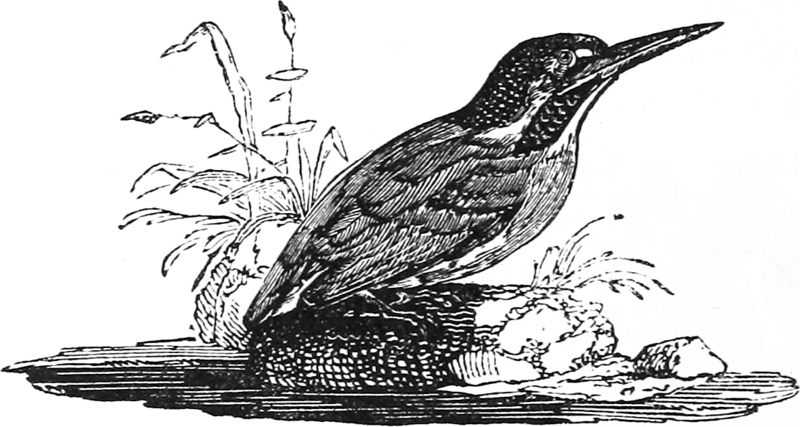
\includegraphics[scale=0.35]{images/Alycon.png}
        \end{figure}
        \vspace{0.5cm}
        \Huge
        \textbf{\textsc{Matematyka Dyskretna}}
        
        \vspace{0.5cm}
        \Large
        \textsc{Wybrane Dowody}
        
        \normalsize
        
        
        \line(1,0){330}
        
        \vspace{1cm}
        \textit{,,Myślę, że 7 punktów na 20 to nie jest zły wynik''}
        \vspace{1cm}

        \textit{\textsc{Popełnione przez}}\\
        \vspace{5mm}

        \textbf{\textsc{Dziurawy Ponton \\ Załatany Ponton \\ Puchaty Pompon \\ Zatopiony Ponton \\ Tonący Ponton \\ Notnop}}

        \vfill

        Kraków \\
        Anno Domini 2023
        
    \end{center}
    
\end{titlepage}


\tableofcontents
\section*{Licencja}
    \begin{figure}[h]
    	\begin{minipage}[c]{0.25\textwidth}
    		
\includegraphics[width=0.7\textwidth]{images/licencja.png}
    	\end{minipage}\hfill
    	\begin{minipage}[c]{0.75\textwidth}
    		\caption*{
    			Ten utwór jest dostępny na 
    			\href{https://creativecommons.org/licenses/by-sa/4.0/}{licencji Creative Commons Uznanie autorstwa
    			na tych samych warunkach 4.0 Międzynarodowe.}
    		}
    	\end{minipage}
    \end{figure}

% Actual content
\mainmatter

\chapter{Kombinatoryka}
 % Żeby nie było syfu to kolejne sekcje dodajemy do chapters/
% A potem includujemy za pomocą \input{chapters/...}

% Używamy \( \) i \[ \] zamiast dolarów -- tak jak się robi w LaTeXu


\documentclass[12pt, a4paper, polish, openany]{book}

% Please, let's familiarize ourselves with notatki.sty and tcs.sty so that we don't reinvent the wheel
\usepackage{notatki}

\fancyhead[L]{\textbf{\textit{MD}}}
\author{
}
\title{TCS and shitposting}


\begin{document}

% Front page and table of contents
\frontmatter

\begin{titlepage} 

    \begin{center}
         \begin{figure}[h]
            \centering
            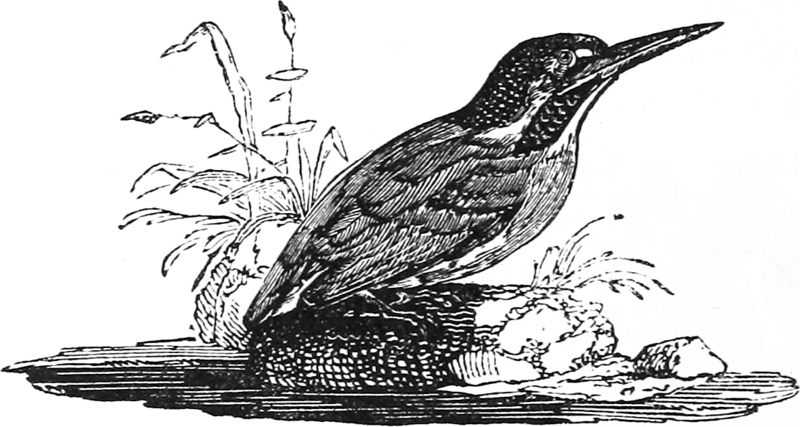
\includegraphics[scale=0.35]{images/Alycon.png}
        \end{figure}
        \vspace{0.5cm}
        \Huge
        \textbf{\textsc{Matematyka Dyskretna}}
        
        \vspace{0.5cm}
        \Large
        \textsc{Wybrane Dowody}
        
        \normalsize
        
        
        \line(1,0){330}
        
        \vspace{1cm}
        \textit{,,Myślę, że 7 punktów na 20 to nie jest zły wynik''}
        \vspace{1cm}

        \textit{\textsc{Popełnione przez}}\\
        \vspace{5mm}

        \textbf{\textsc{Dziurawy Ponton \\ Załatany Ponton \\ Puchaty Pompon \\ Zatopiony Ponton \\ Tonący Ponton \\ Notnop}}

        \vfill

        Kraków \\
        Anno Domini 2023
        
    \end{center}
    
\end{titlepage}


\tableofcontents
\section*{Licencja}
    \begin{figure}[h]
    	\begin{minipage}[c]{0.25\textwidth}
    		
\includegraphics[width=0.7\textwidth]{images/licencja.png}
    	\end{minipage}\hfill
    	\begin{minipage}[c]{0.75\textwidth}
    		\caption*{
    			Ten utwór jest dostępny na 
    			\href{https://creativecommons.org/licenses/by-sa/4.0/}{licencji Creative Commons Uznanie autorstwa
    			na tych samych warunkach 4.0 Międzynarodowe.}
    		}
    	\end{minipage}
    \end{figure}

% Actual content
\mainmatter

\chapter{Kombinatoryka}
 % Żeby nie było syfu to kolejne sekcje dodajemy do chapters/
% A potem includujemy za pomocą \input{chapters/...}

% Używamy \( \) i \[ \] zamiast dolarów -- tak jak się robi w LaTeXu


\documentclass[12pt, a4paper, polish, openany]{book}

% Please, let's familiarize ourselves with notatki.sty and tcs.sty so that we don't reinvent the wheel
\usepackage{notatki}

\fancyhead[L]{\textbf{\textit{MD}}}
\author{
}
\title{TCS and shitposting}


\begin{document}

% Front page and table of contents
\frontmatter

\input{titlepage}

\tableofcontents
\input{license}

% Actual content
\mainmatter

\chapter{Kombinatoryka}
\input{chapters/combinatorics/main}

\chapter{Zasada włączeń i wyłączeń}
\input{chapters/exclusion-inclusion/main}

\chapter{Posety}
\input{chapters/posets/main}

\chapter{Twierdzenie Ramseya}
\input{chapters/ramsey/main}

\chapter{Funkcje tworzące}
\input{chapters/generating_functions/main}

\chapter{Przepływy}
\input{chapters/flows/main}

\chapter{Skojarzenia}
\input{chapters/matchings/main}

\chapter{Kolorowanie grafów}
\input{chapters/graph-coloring/main}

\chapter{Grafy, ale nie kolorowanie}
\input{chapters/graph-misc/main}

\end{document}

\chapter{Zasada włączeń i wyłączeń}
 % Żeby nie było syfu to kolejne sekcje dodajemy do chapters/
% A potem includujemy za pomocą \input{chapters/...}

% Używamy \( \) i \[ \] zamiast dolarów -- tak jak się robi w LaTeXu


\documentclass[12pt, a4paper, polish, openany]{book}

% Please, let's familiarize ourselves with notatki.sty and tcs.sty so that we don't reinvent the wheel
\usepackage{notatki}

\fancyhead[L]{\textbf{\textit{MD}}}
\author{
}
\title{TCS and shitposting}


\begin{document}

% Front page and table of contents
\frontmatter

\input{titlepage}

\tableofcontents
\input{license}

% Actual content
\mainmatter

\chapter{Kombinatoryka}
\input{chapters/combinatorics/main}

\chapter{Zasada włączeń i wyłączeń}
\input{chapters/exclusion-inclusion/main}

\chapter{Posety}
\input{chapters/posets/main}

\chapter{Twierdzenie Ramseya}
\input{chapters/ramsey/main}

\chapter{Funkcje tworzące}
\input{chapters/generating_functions/main}

\chapter{Przepływy}
\input{chapters/flows/main}

\chapter{Skojarzenia}
\input{chapters/matchings/main}

\chapter{Kolorowanie grafów}
\input{chapters/graph-coloring/main}

\chapter{Grafy, ale nie kolorowanie}
\input{chapters/graph-misc/main}

\end{document}

\chapter{Posety}
 % Żeby nie było syfu to kolejne sekcje dodajemy do chapters/
% A potem includujemy za pomocą \input{chapters/...}

% Używamy \( \) i \[ \] zamiast dolarów -- tak jak się robi w LaTeXu


\documentclass[12pt, a4paper, polish, openany]{book}

% Please, let's familiarize ourselves with notatki.sty and tcs.sty so that we don't reinvent the wheel
\usepackage{notatki}

\fancyhead[L]{\textbf{\textit{MD}}}
\author{
}
\title{TCS and shitposting}


\begin{document}

% Front page and table of contents
\frontmatter

\input{titlepage}

\tableofcontents
\input{license}

% Actual content
\mainmatter

\chapter{Kombinatoryka}
\input{chapters/combinatorics/main}

\chapter{Zasada włączeń i wyłączeń}
\input{chapters/exclusion-inclusion/main}

\chapter{Posety}
\input{chapters/posets/main}

\chapter{Twierdzenie Ramseya}
\input{chapters/ramsey/main}

\chapter{Funkcje tworzące}
\input{chapters/generating_functions/main}

\chapter{Przepływy}
\input{chapters/flows/main}

\chapter{Skojarzenia}
\input{chapters/matchings/main}

\chapter{Kolorowanie grafów}
\input{chapters/graph-coloring/main}

\chapter{Grafy, ale nie kolorowanie}
\input{chapters/graph-misc/main}

\end{document}

\chapter{Twierdzenie Ramseya}
 % Żeby nie było syfu to kolejne sekcje dodajemy do chapters/
% A potem includujemy za pomocą \input{chapters/...}

% Używamy \( \) i \[ \] zamiast dolarów -- tak jak się robi w LaTeXu


\documentclass[12pt, a4paper, polish, openany]{book}

% Please, let's familiarize ourselves with notatki.sty and tcs.sty so that we don't reinvent the wheel
\usepackage{notatki}

\fancyhead[L]{\textbf{\textit{MD}}}
\author{
}
\title{TCS and shitposting}


\begin{document}

% Front page and table of contents
\frontmatter

\input{titlepage}

\tableofcontents
\input{license}

% Actual content
\mainmatter

\chapter{Kombinatoryka}
\input{chapters/combinatorics/main}

\chapter{Zasada włączeń i wyłączeń}
\input{chapters/exclusion-inclusion/main}

\chapter{Posety}
\input{chapters/posets/main}

\chapter{Twierdzenie Ramseya}
\input{chapters/ramsey/main}

\chapter{Funkcje tworzące}
\input{chapters/generating_functions/main}

\chapter{Przepływy}
\input{chapters/flows/main}

\chapter{Skojarzenia}
\input{chapters/matchings/main}

\chapter{Kolorowanie grafów}
\input{chapters/graph-coloring/main}

\chapter{Grafy, ale nie kolorowanie}
\input{chapters/graph-misc/main}

\end{document}

\chapter{Funkcje tworzące}
 % Żeby nie było syfu to kolejne sekcje dodajemy do chapters/
% A potem includujemy za pomocą \input{chapters/...}

% Używamy \( \) i \[ \] zamiast dolarów -- tak jak się robi w LaTeXu


\documentclass[12pt, a4paper, polish, openany]{book}

% Please, let's familiarize ourselves with notatki.sty and tcs.sty so that we don't reinvent the wheel
\usepackage{notatki}

\fancyhead[L]{\textbf{\textit{MD}}}
\author{
}
\title{TCS and shitposting}


\begin{document}

% Front page and table of contents
\frontmatter

\input{titlepage}

\tableofcontents
\input{license}

% Actual content
\mainmatter

\chapter{Kombinatoryka}
\input{chapters/combinatorics/main}

\chapter{Zasada włączeń i wyłączeń}
\input{chapters/exclusion-inclusion/main}

\chapter{Posety}
\input{chapters/posets/main}

\chapter{Twierdzenie Ramseya}
\input{chapters/ramsey/main}

\chapter{Funkcje tworzące}
\input{chapters/generating_functions/main}

\chapter{Przepływy}
\input{chapters/flows/main}

\chapter{Skojarzenia}
\input{chapters/matchings/main}

\chapter{Kolorowanie grafów}
\input{chapters/graph-coloring/main}

\chapter{Grafy, ale nie kolorowanie}
\input{chapters/graph-misc/main}

\end{document}

\chapter{Przepływy}
 % Żeby nie było syfu to kolejne sekcje dodajemy do chapters/
% A potem includujemy za pomocą \input{chapters/...}

% Używamy \( \) i \[ \] zamiast dolarów -- tak jak się robi w LaTeXu


\documentclass[12pt, a4paper, polish, openany]{book}

% Please, let's familiarize ourselves with notatki.sty and tcs.sty so that we don't reinvent the wheel
\usepackage{notatki}

\fancyhead[L]{\textbf{\textit{MD}}}
\author{
}
\title{TCS and shitposting}


\begin{document}

% Front page and table of contents
\frontmatter

\input{titlepage}

\tableofcontents
\input{license}

% Actual content
\mainmatter

\chapter{Kombinatoryka}
\input{chapters/combinatorics/main}

\chapter{Zasada włączeń i wyłączeń}
\input{chapters/exclusion-inclusion/main}

\chapter{Posety}
\input{chapters/posets/main}

\chapter{Twierdzenie Ramseya}
\input{chapters/ramsey/main}

\chapter{Funkcje tworzące}
\input{chapters/generating_functions/main}

\chapter{Przepływy}
\input{chapters/flows/main}

\chapter{Skojarzenia}
\input{chapters/matchings/main}

\chapter{Kolorowanie grafów}
\input{chapters/graph-coloring/main}

\chapter{Grafy, ale nie kolorowanie}
\input{chapters/graph-misc/main}

\end{document}

\chapter{Skojarzenia}
 % Żeby nie było syfu to kolejne sekcje dodajemy do chapters/
% A potem includujemy za pomocą \input{chapters/...}

% Używamy \( \) i \[ \] zamiast dolarów -- tak jak się robi w LaTeXu


\documentclass[12pt, a4paper, polish, openany]{book}

% Please, let's familiarize ourselves with notatki.sty and tcs.sty so that we don't reinvent the wheel
\usepackage{notatki}

\fancyhead[L]{\textbf{\textit{MD}}}
\author{
}
\title{TCS and shitposting}


\begin{document}

% Front page and table of contents
\frontmatter

\input{titlepage}

\tableofcontents
\input{license}

% Actual content
\mainmatter

\chapter{Kombinatoryka}
\input{chapters/combinatorics/main}

\chapter{Zasada włączeń i wyłączeń}
\input{chapters/exclusion-inclusion/main}

\chapter{Posety}
\input{chapters/posets/main}

\chapter{Twierdzenie Ramseya}
\input{chapters/ramsey/main}

\chapter{Funkcje tworzące}
\input{chapters/generating_functions/main}

\chapter{Przepływy}
\input{chapters/flows/main}

\chapter{Skojarzenia}
\input{chapters/matchings/main}

\chapter{Kolorowanie grafów}
\input{chapters/graph-coloring/main}

\chapter{Grafy, ale nie kolorowanie}
\input{chapters/graph-misc/main}

\end{document}

\chapter{Kolorowanie grafów}
 % Żeby nie było syfu to kolejne sekcje dodajemy do chapters/
% A potem includujemy za pomocą \input{chapters/...}

% Używamy \( \) i \[ \] zamiast dolarów -- tak jak się robi w LaTeXu


\documentclass[12pt, a4paper, polish, openany]{book}

% Please, let's familiarize ourselves with notatki.sty and tcs.sty so that we don't reinvent the wheel
\usepackage{notatki}

\fancyhead[L]{\textbf{\textit{MD}}}
\author{
}
\title{TCS and shitposting}


\begin{document}

% Front page and table of contents
\frontmatter

\input{titlepage}

\tableofcontents
\input{license}

% Actual content
\mainmatter

\chapter{Kombinatoryka}
\input{chapters/combinatorics/main}

\chapter{Zasada włączeń i wyłączeń}
\input{chapters/exclusion-inclusion/main}

\chapter{Posety}
\input{chapters/posets/main}

\chapter{Twierdzenie Ramseya}
\input{chapters/ramsey/main}

\chapter{Funkcje tworzące}
\input{chapters/generating_functions/main}

\chapter{Przepływy}
\input{chapters/flows/main}

\chapter{Skojarzenia}
\input{chapters/matchings/main}

\chapter{Kolorowanie grafów}
\input{chapters/graph-coloring/main}

\chapter{Grafy, ale nie kolorowanie}
\input{chapters/graph-misc/main}

\end{document}

\chapter{Grafy, ale nie kolorowanie}
 % Żeby nie było syfu to kolejne sekcje dodajemy do chapters/
% A potem includujemy za pomocą \input{chapters/...}

% Używamy \( \) i \[ \] zamiast dolarów -- tak jak się robi w LaTeXu


\documentclass[12pt, a4paper, polish, openany]{book}

% Please, let's familiarize ourselves with notatki.sty and tcs.sty so that we don't reinvent the wheel
\usepackage{notatki}

\fancyhead[L]{\textbf{\textit{MD}}}
\author{
}
\title{TCS and shitposting}


\begin{document}

% Front page and table of contents
\frontmatter

\input{titlepage}

\tableofcontents
\input{license}

% Actual content
\mainmatter

\chapter{Kombinatoryka}
\input{chapters/combinatorics/main}

\chapter{Zasada włączeń i wyłączeń}
\input{chapters/exclusion-inclusion/main}

\chapter{Posety}
\input{chapters/posets/main}

\chapter{Twierdzenie Ramseya}
\input{chapters/ramsey/main}

\chapter{Funkcje tworzące}
\input{chapters/generating_functions/main}

\chapter{Przepływy}
\input{chapters/flows/main}

\chapter{Skojarzenia}
\input{chapters/matchings/main}

\chapter{Kolorowanie grafów}
\input{chapters/graph-coloring/main}

\chapter{Grafy, ale nie kolorowanie}
\input{chapters/graph-misc/main}

\end{document}

\end{document}

\chapter{Zasada włączeń i wyłączeń}
 % Żeby nie było syfu to kolejne sekcje dodajemy do chapters/
% A potem includujemy za pomocą \input{chapters/...}

% Używamy \( \) i \[ \] zamiast dolarów -- tak jak się robi w LaTeXu


\documentclass[12pt, a4paper, polish, openany]{book}

% Please, let's familiarize ourselves with notatki.sty and tcs.sty so that we don't reinvent the wheel
\usepackage{notatki}

\fancyhead[L]{\textbf{\textit{MD}}}
\author{
}
\title{TCS and shitposting}


\begin{document}

% Front page and table of contents
\frontmatter

\begin{titlepage} 

    \begin{center}
         \begin{figure}[h]
            \centering
            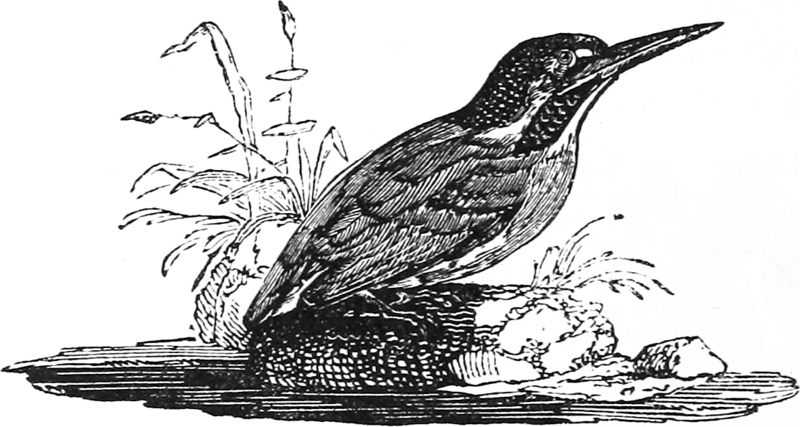
\includegraphics[scale=0.35]{images/Alycon.png}
        \end{figure}
        \vspace{0.5cm}
        \Huge
        \textbf{\textsc{Matematyka Dyskretna}}
        
        \vspace{0.5cm}
        \Large
        \textsc{Wybrane Dowody}
        
        \normalsize
        
        
        \line(1,0){330}
        
        \vspace{1cm}
        \textit{,,Myślę, że 7 punktów na 20 to nie jest zły wynik''}
        \vspace{1cm}

        \textit{\textsc{Popełnione przez}}\\
        \vspace{5mm}

        \textbf{\textsc{Dziurawy Ponton \\ Załatany Ponton \\ Puchaty Pompon \\ Zatopiony Ponton \\ Tonący Ponton \\ Notnop}}

        \vfill

        Kraków \\
        Anno Domini 2023
        
    \end{center}
    
\end{titlepage}


\tableofcontents
\section*{Licencja}
    \begin{figure}[h]
    	\begin{minipage}[c]{0.25\textwidth}
    		
\includegraphics[width=0.7\textwidth]{images/licencja.png}
    	\end{minipage}\hfill
    	\begin{minipage}[c]{0.75\textwidth}
    		\caption*{
    			Ten utwór jest dostępny na 
    			\href{https://creativecommons.org/licenses/by-sa/4.0/}{licencji Creative Commons Uznanie autorstwa
    			na tych samych warunkach 4.0 Międzynarodowe.}
    		}
    	\end{minipage}
    \end{figure}

% Actual content
\mainmatter

\chapter{Kombinatoryka}
 % Żeby nie było syfu to kolejne sekcje dodajemy do chapters/
% A potem includujemy za pomocą \input{chapters/...}

% Używamy \( \) i \[ \] zamiast dolarów -- tak jak się robi w LaTeXu


\documentclass[12pt, a4paper, polish, openany]{book}

% Please, let's familiarize ourselves with notatki.sty and tcs.sty so that we don't reinvent the wheel
\usepackage{notatki}

\fancyhead[L]{\textbf{\textit{MD}}}
\author{
}
\title{TCS and shitposting}


\begin{document}

% Front page and table of contents
\frontmatter

\input{titlepage}

\tableofcontents
\input{license}

% Actual content
\mainmatter

\chapter{Kombinatoryka}
\input{chapters/combinatorics/main}

\chapter{Zasada włączeń i wyłączeń}
\input{chapters/exclusion-inclusion/main}

\chapter{Posety}
\input{chapters/posets/main}

\chapter{Twierdzenie Ramseya}
\input{chapters/ramsey/main}

\chapter{Funkcje tworzące}
\input{chapters/generating_functions/main}

\chapter{Przepływy}
\input{chapters/flows/main}

\chapter{Skojarzenia}
\input{chapters/matchings/main}

\chapter{Kolorowanie grafów}
\input{chapters/graph-coloring/main}

\chapter{Grafy, ale nie kolorowanie}
\input{chapters/graph-misc/main}

\end{document}

\chapter{Zasada włączeń i wyłączeń}
 % Żeby nie było syfu to kolejne sekcje dodajemy do chapters/
% A potem includujemy za pomocą \input{chapters/...}

% Używamy \( \) i \[ \] zamiast dolarów -- tak jak się robi w LaTeXu


\documentclass[12pt, a4paper, polish, openany]{book}

% Please, let's familiarize ourselves with notatki.sty and tcs.sty so that we don't reinvent the wheel
\usepackage{notatki}

\fancyhead[L]{\textbf{\textit{MD}}}
\author{
}
\title{TCS and shitposting}


\begin{document}

% Front page and table of contents
\frontmatter

\input{titlepage}

\tableofcontents
\input{license}

% Actual content
\mainmatter

\chapter{Kombinatoryka}
\input{chapters/combinatorics/main}

\chapter{Zasada włączeń i wyłączeń}
\input{chapters/exclusion-inclusion/main}

\chapter{Posety}
\input{chapters/posets/main}

\chapter{Twierdzenie Ramseya}
\input{chapters/ramsey/main}

\chapter{Funkcje tworzące}
\input{chapters/generating_functions/main}

\chapter{Przepływy}
\input{chapters/flows/main}

\chapter{Skojarzenia}
\input{chapters/matchings/main}

\chapter{Kolorowanie grafów}
\input{chapters/graph-coloring/main}

\chapter{Grafy, ale nie kolorowanie}
\input{chapters/graph-misc/main}

\end{document}

\chapter{Posety}
 % Żeby nie było syfu to kolejne sekcje dodajemy do chapters/
% A potem includujemy za pomocą \input{chapters/...}

% Używamy \( \) i \[ \] zamiast dolarów -- tak jak się robi w LaTeXu


\documentclass[12pt, a4paper, polish, openany]{book}

% Please, let's familiarize ourselves with notatki.sty and tcs.sty so that we don't reinvent the wheel
\usepackage{notatki}

\fancyhead[L]{\textbf{\textit{MD}}}
\author{
}
\title{TCS and shitposting}


\begin{document}

% Front page and table of contents
\frontmatter

\input{titlepage}

\tableofcontents
\input{license}

% Actual content
\mainmatter

\chapter{Kombinatoryka}
\input{chapters/combinatorics/main}

\chapter{Zasada włączeń i wyłączeń}
\input{chapters/exclusion-inclusion/main}

\chapter{Posety}
\input{chapters/posets/main}

\chapter{Twierdzenie Ramseya}
\input{chapters/ramsey/main}

\chapter{Funkcje tworzące}
\input{chapters/generating_functions/main}

\chapter{Przepływy}
\input{chapters/flows/main}

\chapter{Skojarzenia}
\input{chapters/matchings/main}

\chapter{Kolorowanie grafów}
\input{chapters/graph-coloring/main}

\chapter{Grafy, ale nie kolorowanie}
\input{chapters/graph-misc/main}

\end{document}

\chapter{Twierdzenie Ramseya}
 % Żeby nie było syfu to kolejne sekcje dodajemy do chapters/
% A potem includujemy za pomocą \input{chapters/...}

% Używamy \( \) i \[ \] zamiast dolarów -- tak jak się robi w LaTeXu


\documentclass[12pt, a4paper, polish, openany]{book}

% Please, let's familiarize ourselves with notatki.sty and tcs.sty so that we don't reinvent the wheel
\usepackage{notatki}

\fancyhead[L]{\textbf{\textit{MD}}}
\author{
}
\title{TCS and shitposting}


\begin{document}

% Front page and table of contents
\frontmatter

\input{titlepage}

\tableofcontents
\input{license}

% Actual content
\mainmatter

\chapter{Kombinatoryka}
\input{chapters/combinatorics/main}

\chapter{Zasada włączeń i wyłączeń}
\input{chapters/exclusion-inclusion/main}

\chapter{Posety}
\input{chapters/posets/main}

\chapter{Twierdzenie Ramseya}
\input{chapters/ramsey/main}

\chapter{Funkcje tworzące}
\input{chapters/generating_functions/main}

\chapter{Przepływy}
\input{chapters/flows/main}

\chapter{Skojarzenia}
\input{chapters/matchings/main}

\chapter{Kolorowanie grafów}
\input{chapters/graph-coloring/main}

\chapter{Grafy, ale nie kolorowanie}
\input{chapters/graph-misc/main}

\end{document}

\chapter{Funkcje tworzące}
 % Żeby nie było syfu to kolejne sekcje dodajemy do chapters/
% A potem includujemy za pomocą \input{chapters/...}

% Używamy \( \) i \[ \] zamiast dolarów -- tak jak się robi w LaTeXu


\documentclass[12pt, a4paper, polish, openany]{book}

% Please, let's familiarize ourselves with notatki.sty and tcs.sty so that we don't reinvent the wheel
\usepackage{notatki}

\fancyhead[L]{\textbf{\textit{MD}}}
\author{
}
\title{TCS and shitposting}


\begin{document}

% Front page and table of contents
\frontmatter

\input{titlepage}

\tableofcontents
\input{license}

% Actual content
\mainmatter

\chapter{Kombinatoryka}
\input{chapters/combinatorics/main}

\chapter{Zasada włączeń i wyłączeń}
\input{chapters/exclusion-inclusion/main}

\chapter{Posety}
\input{chapters/posets/main}

\chapter{Twierdzenie Ramseya}
\input{chapters/ramsey/main}

\chapter{Funkcje tworzące}
\input{chapters/generating_functions/main}

\chapter{Przepływy}
\input{chapters/flows/main}

\chapter{Skojarzenia}
\input{chapters/matchings/main}

\chapter{Kolorowanie grafów}
\input{chapters/graph-coloring/main}

\chapter{Grafy, ale nie kolorowanie}
\input{chapters/graph-misc/main}

\end{document}

\chapter{Przepływy}
 % Żeby nie było syfu to kolejne sekcje dodajemy do chapters/
% A potem includujemy za pomocą \input{chapters/...}

% Używamy \( \) i \[ \] zamiast dolarów -- tak jak się robi w LaTeXu


\documentclass[12pt, a4paper, polish, openany]{book}

% Please, let's familiarize ourselves with notatki.sty and tcs.sty so that we don't reinvent the wheel
\usepackage{notatki}

\fancyhead[L]{\textbf{\textit{MD}}}
\author{
}
\title{TCS and shitposting}


\begin{document}

% Front page and table of contents
\frontmatter

\input{titlepage}

\tableofcontents
\input{license}

% Actual content
\mainmatter

\chapter{Kombinatoryka}
\input{chapters/combinatorics/main}

\chapter{Zasada włączeń i wyłączeń}
\input{chapters/exclusion-inclusion/main}

\chapter{Posety}
\input{chapters/posets/main}

\chapter{Twierdzenie Ramseya}
\input{chapters/ramsey/main}

\chapter{Funkcje tworzące}
\input{chapters/generating_functions/main}

\chapter{Przepływy}
\input{chapters/flows/main}

\chapter{Skojarzenia}
\input{chapters/matchings/main}

\chapter{Kolorowanie grafów}
\input{chapters/graph-coloring/main}

\chapter{Grafy, ale nie kolorowanie}
\input{chapters/graph-misc/main}

\end{document}

\chapter{Skojarzenia}
 % Żeby nie było syfu to kolejne sekcje dodajemy do chapters/
% A potem includujemy za pomocą \input{chapters/...}

% Używamy \( \) i \[ \] zamiast dolarów -- tak jak się robi w LaTeXu


\documentclass[12pt, a4paper, polish, openany]{book}

% Please, let's familiarize ourselves with notatki.sty and tcs.sty so that we don't reinvent the wheel
\usepackage{notatki}

\fancyhead[L]{\textbf{\textit{MD}}}
\author{
}
\title{TCS and shitposting}


\begin{document}

% Front page and table of contents
\frontmatter

\input{titlepage}

\tableofcontents
\input{license}

% Actual content
\mainmatter

\chapter{Kombinatoryka}
\input{chapters/combinatorics/main}

\chapter{Zasada włączeń i wyłączeń}
\input{chapters/exclusion-inclusion/main}

\chapter{Posety}
\input{chapters/posets/main}

\chapter{Twierdzenie Ramseya}
\input{chapters/ramsey/main}

\chapter{Funkcje tworzące}
\input{chapters/generating_functions/main}

\chapter{Przepływy}
\input{chapters/flows/main}

\chapter{Skojarzenia}
\input{chapters/matchings/main}

\chapter{Kolorowanie grafów}
\input{chapters/graph-coloring/main}

\chapter{Grafy, ale nie kolorowanie}
\input{chapters/graph-misc/main}

\end{document}

\chapter{Kolorowanie grafów}
 % Żeby nie było syfu to kolejne sekcje dodajemy do chapters/
% A potem includujemy za pomocą \input{chapters/...}

% Używamy \( \) i \[ \] zamiast dolarów -- tak jak się robi w LaTeXu


\documentclass[12pt, a4paper, polish, openany]{book}

% Please, let's familiarize ourselves with notatki.sty and tcs.sty so that we don't reinvent the wheel
\usepackage{notatki}

\fancyhead[L]{\textbf{\textit{MD}}}
\author{
}
\title{TCS and shitposting}


\begin{document}

% Front page and table of contents
\frontmatter

\input{titlepage}

\tableofcontents
\input{license}

% Actual content
\mainmatter

\chapter{Kombinatoryka}
\input{chapters/combinatorics/main}

\chapter{Zasada włączeń i wyłączeń}
\input{chapters/exclusion-inclusion/main}

\chapter{Posety}
\input{chapters/posets/main}

\chapter{Twierdzenie Ramseya}
\input{chapters/ramsey/main}

\chapter{Funkcje tworzące}
\input{chapters/generating_functions/main}

\chapter{Przepływy}
\input{chapters/flows/main}

\chapter{Skojarzenia}
\input{chapters/matchings/main}

\chapter{Kolorowanie grafów}
\input{chapters/graph-coloring/main}

\chapter{Grafy, ale nie kolorowanie}
\input{chapters/graph-misc/main}

\end{document}

\chapter{Grafy, ale nie kolorowanie}
 % Żeby nie było syfu to kolejne sekcje dodajemy do chapters/
% A potem includujemy za pomocą \input{chapters/...}

% Używamy \( \) i \[ \] zamiast dolarów -- tak jak się robi w LaTeXu


\documentclass[12pt, a4paper, polish, openany]{book}

% Please, let's familiarize ourselves with notatki.sty and tcs.sty so that we don't reinvent the wheel
\usepackage{notatki}

\fancyhead[L]{\textbf{\textit{MD}}}
\author{
}
\title{TCS and shitposting}


\begin{document}

% Front page and table of contents
\frontmatter

\input{titlepage}

\tableofcontents
\input{license}

% Actual content
\mainmatter

\chapter{Kombinatoryka}
\input{chapters/combinatorics/main}

\chapter{Zasada włączeń i wyłączeń}
\input{chapters/exclusion-inclusion/main}

\chapter{Posety}
\input{chapters/posets/main}

\chapter{Twierdzenie Ramseya}
\input{chapters/ramsey/main}

\chapter{Funkcje tworzące}
\input{chapters/generating_functions/main}

\chapter{Przepływy}
\input{chapters/flows/main}

\chapter{Skojarzenia}
\input{chapters/matchings/main}

\chapter{Kolorowanie grafów}
\input{chapters/graph-coloring/main}

\chapter{Grafy, ale nie kolorowanie}
\input{chapters/graph-misc/main}

\end{document}

\end{document}

\chapter{Posety}
 % Żeby nie było syfu to kolejne sekcje dodajemy do chapters/
% A potem includujemy za pomocą \input{chapters/...}

% Używamy \( \) i \[ \] zamiast dolarów -- tak jak się robi w LaTeXu


\documentclass[12pt, a4paper, polish, openany]{book}

% Please, let's familiarize ourselves with notatki.sty and tcs.sty so that we don't reinvent the wheel
\usepackage{notatki}

\fancyhead[L]{\textbf{\textit{MD}}}
\author{
}
\title{TCS and shitposting}


\begin{document}

% Front page and table of contents
\frontmatter

\begin{titlepage} 

    \begin{center}
         \begin{figure}[h]
            \centering
            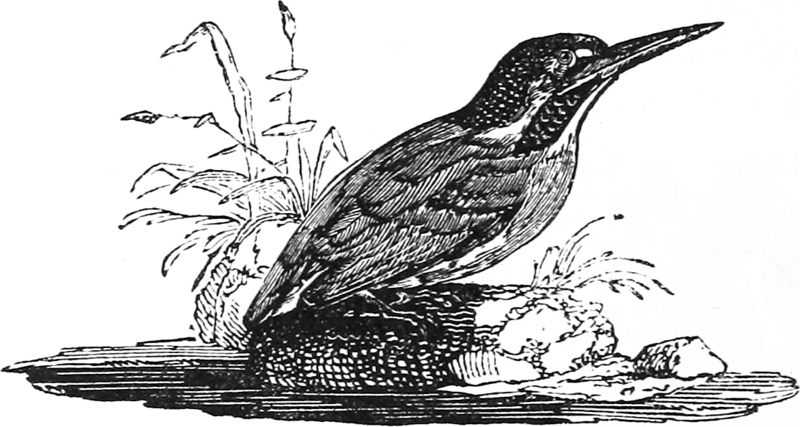
\includegraphics[scale=0.35]{images/Alycon.png}
        \end{figure}
        \vspace{0.5cm}
        \Huge
        \textbf{\textsc{Matematyka Dyskretna}}
        
        \vspace{0.5cm}
        \Large
        \textsc{Wybrane Dowody}
        
        \normalsize
        
        
        \line(1,0){330}
        
        \vspace{1cm}
        \textit{,,Myślę, że 7 punktów na 20 to nie jest zły wynik''}
        \vspace{1cm}

        \textit{\textsc{Popełnione przez}}\\
        \vspace{5mm}

        \textbf{\textsc{Dziurawy Ponton \\ Załatany Ponton \\ Puchaty Pompon \\ Zatopiony Ponton \\ Tonący Ponton \\ Notnop}}

        \vfill

        Kraków \\
        Anno Domini 2023
        
    \end{center}
    
\end{titlepage}


\tableofcontents
\section*{Licencja}
    \begin{figure}[h]
    	\begin{minipage}[c]{0.25\textwidth}
    		
\includegraphics[width=0.7\textwidth]{images/licencja.png}
    	\end{minipage}\hfill
    	\begin{minipage}[c]{0.75\textwidth}
    		\caption*{
    			Ten utwór jest dostępny na 
    			\href{https://creativecommons.org/licenses/by-sa/4.0/}{licencji Creative Commons Uznanie autorstwa
    			na tych samych warunkach 4.0 Międzynarodowe.}
    		}
    	\end{minipage}
    \end{figure}

% Actual content
\mainmatter

\chapter{Kombinatoryka}
 % Żeby nie było syfu to kolejne sekcje dodajemy do chapters/
% A potem includujemy za pomocą \input{chapters/...}

% Używamy \( \) i \[ \] zamiast dolarów -- tak jak się robi w LaTeXu


\documentclass[12pt, a4paper, polish, openany]{book}

% Please, let's familiarize ourselves with notatki.sty and tcs.sty so that we don't reinvent the wheel
\usepackage{notatki}

\fancyhead[L]{\textbf{\textit{MD}}}
\author{
}
\title{TCS and shitposting}


\begin{document}

% Front page and table of contents
\frontmatter

\input{titlepage}

\tableofcontents
\input{license}

% Actual content
\mainmatter

\chapter{Kombinatoryka}
\input{chapters/combinatorics/main}

\chapter{Zasada włączeń i wyłączeń}
\input{chapters/exclusion-inclusion/main}

\chapter{Posety}
\input{chapters/posets/main}

\chapter{Twierdzenie Ramseya}
\input{chapters/ramsey/main}

\chapter{Funkcje tworzące}
\input{chapters/generating_functions/main}

\chapter{Przepływy}
\input{chapters/flows/main}

\chapter{Skojarzenia}
\input{chapters/matchings/main}

\chapter{Kolorowanie grafów}
\input{chapters/graph-coloring/main}

\chapter{Grafy, ale nie kolorowanie}
\input{chapters/graph-misc/main}

\end{document}

\chapter{Zasada włączeń i wyłączeń}
 % Żeby nie było syfu to kolejne sekcje dodajemy do chapters/
% A potem includujemy za pomocą \input{chapters/...}

% Używamy \( \) i \[ \] zamiast dolarów -- tak jak się robi w LaTeXu


\documentclass[12pt, a4paper, polish, openany]{book}

% Please, let's familiarize ourselves with notatki.sty and tcs.sty so that we don't reinvent the wheel
\usepackage{notatki}

\fancyhead[L]{\textbf{\textit{MD}}}
\author{
}
\title{TCS and shitposting}


\begin{document}

% Front page and table of contents
\frontmatter

\input{titlepage}

\tableofcontents
\input{license}

% Actual content
\mainmatter

\chapter{Kombinatoryka}
\input{chapters/combinatorics/main}

\chapter{Zasada włączeń i wyłączeń}
\input{chapters/exclusion-inclusion/main}

\chapter{Posety}
\input{chapters/posets/main}

\chapter{Twierdzenie Ramseya}
\input{chapters/ramsey/main}

\chapter{Funkcje tworzące}
\input{chapters/generating_functions/main}

\chapter{Przepływy}
\input{chapters/flows/main}

\chapter{Skojarzenia}
\input{chapters/matchings/main}

\chapter{Kolorowanie grafów}
\input{chapters/graph-coloring/main}

\chapter{Grafy, ale nie kolorowanie}
\input{chapters/graph-misc/main}

\end{document}

\chapter{Posety}
 % Żeby nie było syfu to kolejne sekcje dodajemy do chapters/
% A potem includujemy za pomocą \input{chapters/...}

% Używamy \( \) i \[ \] zamiast dolarów -- tak jak się robi w LaTeXu


\documentclass[12pt, a4paper, polish, openany]{book}

% Please, let's familiarize ourselves with notatki.sty and tcs.sty so that we don't reinvent the wheel
\usepackage{notatki}

\fancyhead[L]{\textbf{\textit{MD}}}
\author{
}
\title{TCS and shitposting}


\begin{document}

% Front page and table of contents
\frontmatter

\input{titlepage}

\tableofcontents
\input{license}

% Actual content
\mainmatter

\chapter{Kombinatoryka}
\input{chapters/combinatorics/main}

\chapter{Zasada włączeń i wyłączeń}
\input{chapters/exclusion-inclusion/main}

\chapter{Posety}
\input{chapters/posets/main}

\chapter{Twierdzenie Ramseya}
\input{chapters/ramsey/main}

\chapter{Funkcje tworzące}
\input{chapters/generating_functions/main}

\chapter{Przepływy}
\input{chapters/flows/main}

\chapter{Skojarzenia}
\input{chapters/matchings/main}

\chapter{Kolorowanie grafów}
\input{chapters/graph-coloring/main}

\chapter{Grafy, ale nie kolorowanie}
\input{chapters/graph-misc/main}

\end{document}

\chapter{Twierdzenie Ramseya}
 % Żeby nie było syfu to kolejne sekcje dodajemy do chapters/
% A potem includujemy za pomocą \input{chapters/...}

% Używamy \( \) i \[ \] zamiast dolarów -- tak jak się robi w LaTeXu


\documentclass[12pt, a4paper, polish, openany]{book}

% Please, let's familiarize ourselves with notatki.sty and tcs.sty so that we don't reinvent the wheel
\usepackage{notatki}

\fancyhead[L]{\textbf{\textit{MD}}}
\author{
}
\title{TCS and shitposting}


\begin{document}

% Front page and table of contents
\frontmatter

\input{titlepage}

\tableofcontents
\input{license}

% Actual content
\mainmatter

\chapter{Kombinatoryka}
\input{chapters/combinatorics/main}

\chapter{Zasada włączeń i wyłączeń}
\input{chapters/exclusion-inclusion/main}

\chapter{Posety}
\input{chapters/posets/main}

\chapter{Twierdzenie Ramseya}
\input{chapters/ramsey/main}

\chapter{Funkcje tworzące}
\input{chapters/generating_functions/main}

\chapter{Przepływy}
\input{chapters/flows/main}

\chapter{Skojarzenia}
\input{chapters/matchings/main}

\chapter{Kolorowanie grafów}
\input{chapters/graph-coloring/main}

\chapter{Grafy, ale nie kolorowanie}
\input{chapters/graph-misc/main}

\end{document}

\chapter{Funkcje tworzące}
 % Żeby nie było syfu to kolejne sekcje dodajemy do chapters/
% A potem includujemy za pomocą \input{chapters/...}

% Używamy \( \) i \[ \] zamiast dolarów -- tak jak się robi w LaTeXu


\documentclass[12pt, a4paper, polish, openany]{book}

% Please, let's familiarize ourselves with notatki.sty and tcs.sty so that we don't reinvent the wheel
\usepackage{notatki}

\fancyhead[L]{\textbf{\textit{MD}}}
\author{
}
\title{TCS and shitposting}


\begin{document}

% Front page and table of contents
\frontmatter

\input{titlepage}

\tableofcontents
\input{license}

% Actual content
\mainmatter

\chapter{Kombinatoryka}
\input{chapters/combinatorics/main}

\chapter{Zasada włączeń i wyłączeń}
\input{chapters/exclusion-inclusion/main}

\chapter{Posety}
\input{chapters/posets/main}

\chapter{Twierdzenie Ramseya}
\input{chapters/ramsey/main}

\chapter{Funkcje tworzące}
\input{chapters/generating_functions/main}

\chapter{Przepływy}
\input{chapters/flows/main}

\chapter{Skojarzenia}
\input{chapters/matchings/main}

\chapter{Kolorowanie grafów}
\input{chapters/graph-coloring/main}

\chapter{Grafy, ale nie kolorowanie}
\input{chapters/graph-misc/main}

\end{document}

\chapter{Przepływy}
 % Żeby nie było syfu to kolejne sekcje dodajemy do chapters/
% A potem includujemy za pomocą \input{chapters/...}

% Używamy \( \) i \[ \] zamiast dolarów -- tak jak się robi w LaTeXu


\documentclass[12pt, a4paper, polish, openany]{book}

% Please, let's familiarize ourselves with notatki.sty and tcs.sty so that we don't reinvent the wheel
\usepackage{notatki}

\fancyhead[L]{\textbf{\textit{MD}}}
\author{
}
\title{TCS and shitposting}


\begin{document}

% Front page and table of contents
\frontmatter

\input{titlepage}

\tableofcontents
\input{license}

% Actual content
\mainmatter

\chapter{Kombinatoryka}
\input{chapters/combinatorics/main}

\chapter{Zasada włączeń i wyłączeń}
\input{chapters/exclusion-inclusion/main}

\chapter{Posety}
\input{chapters/posets/main}

\chapter{Twierdzenie Ramseya}
\input{chapters/ramsey/main}

\chapter{Funkcje tworzące}
\input{chapters/generating_functions/main}

\chapter{Przepływy}
\input{chapters/flows/main}

\chapter{Skojarzenia}
\input{chapters/matchings/main}

\chapter{Kolorowanie grafów}
\input{chapters/graph-coloring/main}

\chapter{Grafy, ale nie kolorowanie}
\input{chapters/graph-misc/main}

\end{document}

\chapter{Skojarzenia}
 % Żeby nie było syfu to kolejne sekcje dodajemy do chapters/
% A potem includujemy za pomocą \input{chapters/...}

% Używamy \( \) i \[ \] zamiast dolarów -- tak jak się robi w LaTeXu


\documentclass[12pt, a4paper, polish, openany]{book}

% Please, let's familiarize ourselves with notatki.sty and tcs.sty so that we don't reinvent the wheel
\usepackage{notatki}

\fancyhead[L]{\textbf{\textit{MD}}}
\author{
}
\title{TCS and shitposting}


\begin{document}

% Front page and table of contents
\frontmatter

\input{titlepage}

\tableofcontents
\input{license}

% Actual content
\mainmatter

\chapter{Kombinatoryka}
\input{chapters/combinatorics/main}

\chapter{Zasada włączeń i wyłączeń}
\input{chapters/exclusion-inclusion/main}

\chapter{Posety}
\input{chapters/posets/main}

\chapter{Twierdzenie Ramseya}
\input{chapters/ramsey/main}

\chapter{Funkcje tworzące}
\input{chapters/generating_functions/main}

\chapter{Przepływy}
\input{chapters/flows/main}

\chapter{Skojarzenia}
\input{chapters/matchings/main}

\chapter{Kolorowanie grafów}
\input{chapters/graph-coloring/main}

\chapter{Grafy, ale nie kolorowanie}
\input{chapters/graph-misc/main}

\end{document}

\chapter{Kolorowanie grafów}
 % Żeby nie było syfu to kolejne sekcje dodajemy do chapters/
% A potem includujemy za pomocą \input{chapters/...}

% Używamy \( \) i \[ \] zamiast dolarów -- tak jak się robi w LaTeXu


\documentclass[12pt, a4paper, polish, openany]{book}

% Please, let's familiarize ourselves with notatki.sty and tcs.sty so that we don't reinvent the wheel
\usepackage{notatki}

\fancyhead[L]{\textbf{\textit{MD}}}
\author{
}
\title{TCS and shitposting}


\begin{document}

% Front page and table of contents
\frontmatter

\input{titlepage}

\tableofcontents
\input{license}

% Actual content
\mainmatter

\chapter{Kombinatoryka}
\input{chapters/combinatorics/main}

\chapter{Zasada włączeń i wyłączeń}
\input{chapters/exclusion-inclusion/main}

\chapter{Posety}
\input{chapters/posets/main}

\chapter{Twierdzenie Ramseya}
\input{chapters/ramsey/main}

\chapter{Funkcje tworzące}
\input{chapters/generating_functions/main}

\chapter{Przepływy}
\input{chapters/flows/main}

\chapter{Skojarzenia}
\input{chapters/matchings/main}

\chapter{Kolorowanie grafów}
\input{chapters/graph-coloring/main}

\chapter{Grafy, ale nie kolorowanie}
\input{chapters/graph-misc/main}

\end{document}

\chapter{Grafy, ale nie kolorowanie}
 % Żeby nie było syfu to kolejne sekcje dodajemy do chapters/
% A potem includujemy za pomocą \input{chapters/...}

% Używamy \( \) i \[ \] zamiast dolarów -- tak jak się robi w LaTeXu


\documentclass[12pt, a4paper, polish, openany]{book}

% Please, let's familiarize ourselves with notatki.sty and tcs.sty so that we don't reinvent the wheel
\usepackage{notatki}

\fancyhead[L]{\textbf{\textit{MD}}}
\author{
}
\title{TCS and shitposting}


\begin{document}

% Front page and table of contents
\frontmatter

\input{titlepage}

\tableofcontents
\input{license}

% Actual content
\mainmatter

\chapter{Kombinatoryka}
\input{chapters/combinatorics/main}

\chapter{Zasada włączeń i wyłączeń}
\input{chapters/exclusion-inclusion/main}

\chapter{Posety}
\input{chapters/posets/main}

\chapter{Twierdzenie Ramseya}
\input{chapters/ramsey/main}

\chapter{Funkcje tworzące}
\input{chapters/generating_functions/main}

\chapter{Przepływy}
\input{chapters/flows/main}

\chapter{Skojarzenia}
\input{chapters/matchings/main}

\chapter{Kolorowanie grafów}
\input{chapters/graph-coloring/main}

\chapter{Grafy, ale nie kolorowanie}
\input{chapters/graph-misc/main}

\end{document}

\end{document}

\chapter{Twierdzenie Ramseya}
 % Żeby nie było syfu to kolejne sekcje dodajemy do chapters/
% A potem includujemy za pomocą \input{chapters/...}

% Używamy \( \) i \[ \] zamiast dolarów -- tak jak się robi w LaTeXu


\documentclass[12pt, a4paper, polish, openany]{book}

% Please, let's familiarize ourselves with notatki.sty and tcs.sty so that we don't reinvent the wheel
\usepackage{notatki}

\fancyhead[L]{\textbf{\textit{MD}}}
\author{
}
\title{TCS and shitposting}


\begin{document}

% Front page and table of contents
\frontmatter

\begin{titlepage} 

    \begin{center}
         \begin{figure}[h]
            \centering
            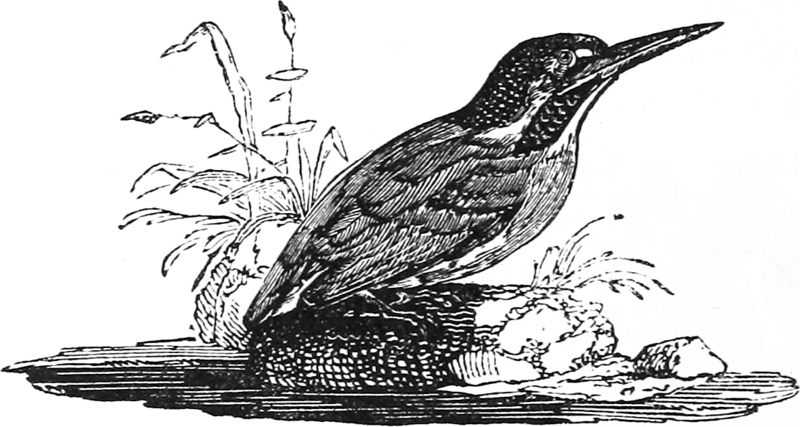
\includegraphics[scale=0.35]{images/Alycon.png}
        \end{figure}
        \vspace{0.5cm}
        \Huge
        \textbf{\textsc{Matematyka Dyskretna}}
        
        \vspace{0.5cm}
        \Large
        \textsc{Wybrane Dowody}
        
        \normalsize
        
        
        \line(1,0){330}
        
        \vspace{1cm}
        \textit{,,Myślę, że 7 punktów na 20 to nie jest zły wynik''}
        \vspace{1cm}

        \textit{\textsc{Popełnione przez}}\\
        \vspace{5mm}

        \textbf{\textsc{Dziurawy Ponton \\ Załatany Ponton \\ Puchaty Pompon \\ Zatopiony Ponton \\ Tonący Ponton \\ Notnop}}

        \vfill

        Kraków \\
        Anno Domini 2023
        
    \end{center}
    
\end{titlepage}


\tableofcontents
\section*{Licencja}
    \begin{figure}[h]
    	\begin{minipage}[c]{0.25\textwidth}
    		
\includegraphics[width=0.7\textwidth]{images/licencja.png}
    	\end{minipage}\hfill
    	\begin{minipage}[c]{0.75\textwidth}
    		\caption*{
    			Ten utwór jest dostępny na 
    			\href{https://creativecommons.org/licenses/by-sa/4.0/}{licencji Creative Commons Uznanie autorstwa
    			na tych samych warunkach 4.0 Międzynarodowe.}
    		}
    	\end{minipage}
    \end{figure}

% Actual content
\mainmatter

\chapter{Kombinatoryka}
 % Żeby nie było syfu to kolejne sekcje dodajemy do chapters/
% A potem includujemy za pomocą \input{chapters/...}

% Używamy \( \) i \[ \] zamiast dolarów -- tak jak się robi w LaTeXu


\documentclass[12pt, a4paper, polish, openany]{book}

% Please, let's familiarize ourselves with notatki.sty and tcs.sty so that we don't reinvent the wheel
\usepackage{notatki}

\fancyhead[L]{\textbf{\textit{MD}}}
\author{
}
\title{TCS and shitposting}


\begin{document}

% Front page and table of contents
\frontmatter

\input{titlepage}

\tableofcontents
\input{license}

% Actual content
\mainmatter

\chapter{Kombinatoryka}
\input{chapters/combinatorics/main}

\chapter{Zasada włączeń i wyłączeń}
\input{chapters/exclusion-inclusion/main}

\chapter{Posety}
\input{chapters/posets/main}

\chapter{Twierdzenie Ramseya}
\input{chapters/ramsey/main}

\chapter{Funkcje tworzące}
\input{chapters/generating_functions/main}

\chapter{Przepływy}
\input{chapters/flows/main}

\chapter{Skojarzenia}
\input{chapters/matchings/main}

\chapter{Kolorowanie grafów}
\input{chapters/graph-coloring/main}

\chapter{Grafy, ale nie kolorowanie}
\input{chapters/graph-misc/main}

\end{document}

\chapter{Zasada włączeń i wyłączeń}
 % Żeby nie było syfu to kolejne sekcje dodajemy do chapters/
% A potem includujemy za pomocą \input{chapters/...}

% Używamy \( \) i \[ \] zamiast dolarów -- tak jak się robi w LaTeXu


\documentclass[12pt, a4paper, polish, openany]{book}

% Please, let's familiarize ourselves with notatki.sty and tcs.sty so that we don't reinvent the wheel
\usepackage{notatki}

\fancyhead[L]{\textbf{\textit{MD}}}
\author{
}
\title{TCS and shitposting}


\begin{document}

% Front page and table of contents
\frontmatter

\input{titlepage}

\tableofcontents
\input{license}

% Actual content
\mainmatter

\chapter{Kombinatoryka}
\input{chapters/combinatorics/main}

\chapter{Zasada włączeń i wyłączeń}
\input{chapters/exclusion-inclusion/main}

\chapter{Posety}
\input{chapters/posets/main}

\chapter{Twierdzenie Ramseya}
\input{chapters/ramsey/main}

\chapter{Funkcje tworzące}
\input{chapters/generating_functions/main}

\chapter{Przepływy}
\input{chapters/flows/main}

\chapter{Skojarzenia}
\input{chapters/matchings/main}

\chapter{Kolorowanie grafów}
\input{chapters/graph-coloring/main}

\chapter{Grafy, ale nie kolorowanie}
\input{chapters/graph-misc/main}

\end{document}

\chapter{Posety}
 % Żeby nie było syfu to kolejne sekcje dodajemy do chapters/
% A potem includujemy za pomocą \input{chapters/...}

% Używamy \( \) i \[ \] zamiast dolarów -- tak jak się robi w LaTeXu


\documentclass[12pt, a4paper, polish, openany]{book}

% Please, let's familiarize ourselves with notatki.sty and tcs.sty so that we don't reinvent the wheel
\usepackage{notatki}

\fancyhead[L]{\textbf{\textit{MD}}}
\author{
}
\title{TCS and shitposting}


\begin{document}

% Front page and table of contents
\frontmatter

\input{titlepage}

\tableofcontents
\input{license}

% Actual content
\mainmatter

\chapter{Kombinatoryka}
\input{chapters/combinatorics/main}

\chapter{Zasada włączeń i wyłączeń}
\input{chapters/exclusion-inclusion/main}

\chapter{Posety}
\input{chapters/posets/main}

\chapter{Twierdzenie Ramseya}
\input{chapters/ramsey/main}

\chapter{Funkcje tworzące}
\input{chapters/generating_functions/main}

\chapter{Przepływy}
\input{chapters/flows/main}

\chapter{Skojarzenia}
\input{chapters/matchings/main}

\chapter{Kolorowanie grafów}
\input{chapters/graph-coloring/main}

\chapter{Grafy, ale nie kolorowanie}
\input{chapters/graph-misc/main}

\end{document}

\chapter{Twierdzenie Ramseya}
 % Żeby nie było syfu to kolejne sekcje dodajemy do chapters/
% A potem includujemy za pomocą \input{chapters/...}

% Używamy \( \) i \[ \] zamiast dolarów -- tak jak się robi w LaTeXu


\documentclass[12pt, a4paper, polish, openany]{book}

% Please, let's familiarize ourselves with notatki.sty and tcs.sty so that we don't reinvent the wheel
\usepackage{notatki}

\fancyhead[L]{\textbf{\textit{MD}}}
\author{
}
\title{TCS and shitposting}


\begin{document}

% Front page and table of contents
\frontmatter

\input{titlepage}

\tableofcontents
\input{license}

% Actual content
\mainmatter

\chapter{Kombinatoryka}
\input{chapters/combinatorics/main}

\chapter{Zasada włączeń i wyłączeń}
\input{chapters/exclusion-inclusion/main}

\chapter{Posety}
\input{chapters/posets/main}

\chapter{Twierdzenie Ramseya}
\input{chapters/ramsey/main}

\chapter{Funkcje tworzące}
\input{chapters/generating_functions/main}

\chapter{Przepływy}
\input{chapters/flows/main}

\chapter{Skojarzenia}
\input{chapters/matchings/main}

\chapter{Kolorowanie grafów}
\input{chapters/graph-coloring/main}

\chapter{Grafy, ale nie kolorowanie}
\input{chapters/graph-misc/main}

\end{document}

\chapter{Funkcje tworzące}
 % Żeby nie było syfu to kolejne sekcje dodajemy do chapters/
% A potem includujemy za pomocą \input{chapters/...}

% Używamy \( \) i \[ \] zamiast dolarów -- tak jak się robi w LaTeXu


\documentclass[12pt, a4paper, polish, openany]{book}

% Please, let's familiarize ourselves with notatki.sty and tcs.sty so that we don't reinvent the wheel
\usepackage{notatki}

\fancyhead[L]{\textbf{\textit{MD}}}
\author{
}
\title{TCS and shitposting}


\begin{document}

% Front page and table of contents
\frontmatter

\input{titlepage}

\tableofcontents
\input{license}

% Actual content
\mainmatter

\chapter{Kombinatoryka}
\input{chapters/combinatorics/main}

\chapter{Zasada włączeń i wyłączeń}
\input{chapters/exclusion-inclusion/main}

\chapter{Posety}
\input{chapters/posets/main}

\chapter{Twierdzenie Ramseya}
\input{chapters/ramsey/main}

\chapter{Funkcje tworzące}
\input{chapters/generating_functions/main}

\chapter{Przepływy}
\input{chapters/flows/main}

\chapter{Skojarzenia}
\input{chapters/matchings/main}

\chapter{Kolorowanie grafów}
\input{chapters/graph-coloring/main}

\chapter{Grafy, ale nie kolorowanie}
\input{chapters/graph-misc/main}

\end{document}

\chapter{Przepływy}
 % Żeby nie było syfu to kolejne sekcje dodajemy do chapters/
% A potem includujemy za pomocą \input{chapters/...}

% Używamy \( \) i \[ \] zamiast dolarów -- tak jak się robi w LaTeXu


\documentclass[12pt, a4paper, polish, openany]{book}

% Please, let's familiarize ourselves with notatki.sty and tcs.sty so that we don't reinvent the wheel
\usepackage{notatki}

\fancyhead[L]{\textbf{\textit{MD}}}
\author{
}
\title{TCS and shitposting}


\begin{document}

% Front page and table of contents
\frontmatter

\input{titlepage}

\tableofcontents
\input{license}

% Actual content
\mainmatter

\chapter{Kombinatoryka}
\input{chapters/combinatorics/main}

\chapter{Zasada włączeń i wyłączeń}
\input{chapters/exclusion-inclusion/main}

\chapter{Posety}
\input{chapters/posets/main}

\chapter{Twierdzenie Ramseya}
\input{chapters/ramsey/main}

\chapter{Funkcje tworzące}
\input{chapters/generating_functions/main}

\chapter{Przepływy}
\input{chapters/flows/main}

\chapter{Skojarzenia}
\input{chapters/matchings/main}

\chapter{Kolorowanie grafów}
\input{chapters/graph-coloring/main}

\chapter{Grafy, ale nie kolorowanie}
\input{chapters/graph-misc/main}

\end{document}

\chapter{Skojarzenia}
 % Żeby nie było syfu to kolejne sekcje dodajemy do chapters/
% A potem includujemy za pomocą \input{chapters/...}

% Używamy \( \) i \[ \] zamiast dolarów -- tak jak się robi w LaTeXu


\documentclass[12pt, a4paper, polish, openany]{book}

% Please, let's familiarize ourselves with notatki.sty and tcs.sty so that we don't reinvent the wheel
\usepackage{notatki}

\fancyhead[L]{\textbf{\textit{MD}}}
\author{
}
\title{TCS and shitposting}


\begin{document}

% Front page and table of contents
\frontmatter

\input{titlepage}

\tableofcontents
\input{license}

% Actual content
\mainmatter

\chapter{Kombinatoryka}
\input{chapters/combinatorics/main}

\chapter{Zasada włączeń i wyłączeń}
\input{chapters/exclusion-inclusion/main}

\chapter{Posety}
\input{chapters/posets/main}

\chapter{Twierdzenie Ramseya}
\input{chapters/ramsey/main}

\chapter{Funkcje tworzące}
\input{chapters/generating_functions/main}

\chapter{Przepływy}
\input{chapters/flows/main}

\chapter{Skojarzenia}
\input{chapters/matchings/main}

\chapter{Kolorowanie grafów}
\input{chapters/graph-coloring/main}

\chapter{Grafy, ale nie kolorowanie}
\input{chapters/graph-misc/main}

\end{document}

\chapter{Kolorowanie grafów}
 % Żeby nie było syfu to kolejne sekcje dodajemy do chapters/
% A potem includujemy za pomocą \input{chapters/...}

% Używamy \( \) i \[ \] zamiast dolarów -- tak jak się robi w LaTeXu


\documentclass[12pt, a4paper, polish, openany]{book}

% Please, let's familiarize ourselves with notatki.sty and tcs.sty so that we don't reinvent the wheel
\usepackage{notatki}

\fancyhead[L]{\textbf{\textit{MD}}}
\author{
}
\title{TCS and shitposting}


\begin{document}

% Front page and table of contents
\frontmatter

\input{titlepage}

\tableofcontents
\input{license}

% Actual content
\mainmatter

\chapter{Kombinatoryka}
\input{chapters/combinatorics/main}

\chapter{Zasada włączeń i wyłączeń}
\input{chapters/exclusion-inclusion/main}

\chapter{Posety}
\input{chapters/posets/main}

\chapter{Twierdzenie Ramseya}
\input{chapters/ramsey/main}

\chapter{Funkcje tworzące}
\input{chapters/generating_functions/main}

\chapter{Przepływy}
\input{chapters/flows/main}

\chapter{Skojarzenia}
\input{chapters/matchings/main}

\chapter{Kolorowanie grafów}
\input{chapters/graph-coloring/main}

\chapter{Grafy, ale nie kolorowanie}
\input{chapters/graph-misc/main}

\end{document}

\chapter{Grafy, ale nie kolorowanie}
 % Żeby nie było syfu to kolejne sekcje dodajemy do chapters/
% A potem includujemy za pomocą \input{chapters/...}

% Używamy \( \) i \[ \] zamiast dolarów -- tak jak się robi w LaTeXu


\documentclass[12pt, a4paper, polish, openany]{book}

% Please, let's familiarize ourselves with notatki.sty and tcs.sty so that we don't reinvent the wheel
\usepackage{notatki}

\fancyhead[L]{\textbf{\textit{MD}}}
\author{
}
\title{TCS and shitposting}


\begin{document}

% Front page and table of contents
\frontmatter

\input{titlepage}

\tableofcontents
\input{license}

% Actual content
\mainmatter

\chapter{Kombinatoryka}
\input{chapters/combinatorics/main}

\chapter{Zasada włączeń i wyłączeń}
\input{chapters/exclusion-inclusion/main}

\chapter{Posety}
\input{chapters/posets/main}

\chapter{Twierdzenie Ramseya}
\input{chapters/ramsey/main}

\chapter{Funkcje tworzące}
\input{chapters/generating_functions/main}

\chapter{Przepływy}
\input{chapters/flows/main}

\chapter{Skojarzenia}
\input{chapters/matchings/main}

\chapter{Kolorowanie grafów}
\input{chapters/graph-coloring/main}

\chapter{Grafy, ale nie kolorowanie}
\input{chapters/graph-misc/main}

\end{document}

\end{document}

\chapter{Funkcje tworzące}
 % Żeby nie było syfu to kolejne sekcje dodajemy do chapters/
% A potem includujemy za pomocą \input{chapters/...}

% Używamy \( \) i \[ \] zamiast dolarów -- tak jak się robi w LaTeXu


\documentclass[12pt, a4paper, polish, openany]{book}

% Please, let's familiarize ourselves with notatki.sty and tcs.sty so that we don't reinvent the wheel
\usepackage{notatki}

\fancyhead[L]{\textbf{\textit{MD}}}
\author{
}
\title{TCS and shitposting}


\begin{document}

% Front page and table of contents
\frontmatter

\begin{titlepage} 

    \begin{center}
         \begin{figure}[h]
            \centering
            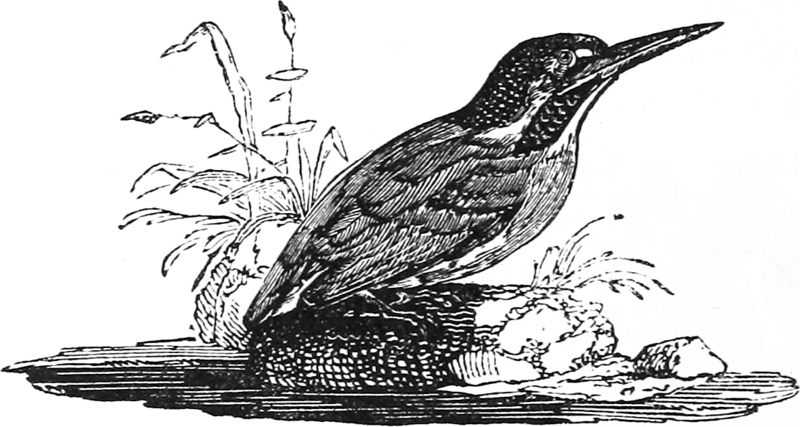
\includegraphics[scale=0.35]{images/Alycon.png}
        \end{figure}
        \vspace{0.5cm}
        \Huge
        \textbf{\textsc{Matematyka Dyskretna}}
        
        \vspace{0.5cm}
        \Large
        \textsc{Wybrane Dowody}
        
        \normalsize
        
        
        \line(1,0){330}
        
        \vspace{1cm}
        \textit{,,Myślę, że 7 punktów na 20 to nie jest zły wynik''}
        \vspace{1cm}

        \textit{\textsc{Popełnione przez}}\\
        \vspace{5mm}

        \textbf{\textsc{Dziurawy Ponton \\ Załatany Ponton \\ Puchaty Pompon \\ Zatopiony Ponton \\ Tonący Ponton \\ Notnop}}

        \vfill

        Kraków \\
        Anno Domini 2023
        
    \end{center}
    
\end{titlepage}


\tableofcontents
\section*{Licencja}
    \begin{figure}[h]
    	\begin{minipage}[c]{0.25\textwidth}
    		
\includegraphics[width=0.7\textwidth]{images/licencja.png}
    	\end{minipage}\hfill
    	\begin{minipage}[c]{0.75\textwidth}
    		\caption*{
    			Ten utwór jest dostępny na 
    			\href{https://creativecommons.org/licenses/by-sa/4.0/}{licencji Creative Commons Uznanie autorstwa
    			na tych samych warunkach 4.0 Międzynarodowe.}
    		}
    	\end{minipage}
    \end{figure}

% Actual content
\mainmatter

\chapter{Kombinatoryka}
 % Żeby nie było syfu to kolejne sekcje dodajemy do chapters/
% A potem includujemy za pomocą \input{chapters/...}

% Używamy \( \) i \[ \] zamiast dolarów -- tak jak się robi w LaTeXu


\documentclass[12pt, a4paper, polish, openany]{book}

% Please, let's familiarize ourselves with notatki.sty and tcs.sty so that we don't reinvent the wheel
\usepackage{notatki}

\fancyhead[L]{\textbf{\textit{MD}}}
\author{
}
\title{TCS and shitposting}


\begin{document}

% Front page and table of contents
\frontmatter

\input{titlepage}

\tableofcontents
\input{license}

% Actual content
\mainmatter

\chapter{Kombinatoryka}
\input{chapters/combinatorics/main}

\chapter{Zasada włączeń i wyłączeń}
\input{chapters/exclusion-inclusion/main}

\chapter{Posety}
\input{chapters/posets/main}

\chapter{Twierdzenie Ramseya}
\input{chapters/ramsey/main}

\chapter{Funkcje tworzące}
\input{chapters/generating_functions/main}

\chapter{Przepływy}
\input{chapters/flows/main}

\chapter{Skojarzenia}
\input{chapters/matchings/main}

\chapter{Kolorowanie grafów}
\input{chapters/graph-coloring/main}

\chapter{Grafy, ale nie kolorowanie}
\input{chapters/graph-misc/main}

\end{document}

\chapter{Zasada włączeń i wyłączeń}
 % Żeby nie było syfu to kolejne sekcje dodajemy do chapters/
% A potem includujemy za pomocą \input{chapters/...}

% Używamy \( \) i \[ \] zamiast dolarów -- tak jak się robi w LaTeXu


\documentclass[12pt, a4paper, polish, openany]{book}

% Please, let's familiarize ourselves with notatki.sty and tcs.sty so that we don't reinvent the wheel
\usepackage{notatki}

\fancyhead[L]{\textbf{\textit{MD}}}
\author{
}
\title{TCS and shitposting}


\begin{document}

% Front page and table of contents
\frontmatter

\input{titlepage}

\tableofcontents
\input{license}

% Actual content
\mainmatter

\chapter{Kombinatoryka}
\input{chapters/combinatorics/main}

\chapter{Zasada włączeń i wyłączeń}
\input{chapters/exclusion-inclusion/main}

\chapter{Posety}
\input{chapters/posets/main}

\chapter{Twierdzenie Ramseya}
\input{chapters/ramsey/main}

\chapter{Funkcje tworzące}
\input{chapters/generating_functions/main}

\chapter{Przepływy}
\input{chapters/flows/main}

\chapter{Skojarzenia}
\input{chapters/matchings/main}

\chapter{Kolorowanie grafów}
\input{chapters/graph-coloring/main}

\chapter{Grafy, ale nie kolorowanie}
\input{chapters/graph-misc/main}

\end{document}

\chapter{Posety}
 % Żeby nie było syfu to kolejne sekcje dodajemy do chapters/
% A potem includujemy za pomocą \input{chapters/...}

% Używamy \( \) i \[ \] zamiast dolarów -- tak jak się robi w LaTeXu


\documentclass[12pt, a4paper, polish, openany]{book}

% Please, let's familiarize ourselves with notatki.sty and tcs.sty so that we don't reinvent the wheel
\usepackage{notatki}

\fancyhead[L]{\textbf{\textit{MD}}}
\author{
}
\title{TCS and shitposting}


\begin{document}

% Front page and table of contents
\frontmatter

\input{titlepage}

\tableofcontents
\input{license}

% Actual content
\mainmatter

\chapter{Kombinatoryka}
\input{chapters/combinatorics/main}

\chapter{Zasada włączeń i wyłączeń}
\input{chapters/exclusion-inclusion/main}

\chapter{Posety}
\input{chapters/posets/main}

\chapter{Twierdzenie Ramseya}
\input{chapters/ramsey/main}

\chapter{Funkcje tworzące}
\input{chapters/generating_functions/main}

\chapter{Przepływy}
\input{chapters/flows/main}

\chapter{Skojarzenia}
\input{chapters/matchings/main}

\chapter{Kolorowanie grafów}
\input{chapters/graph-coloring/main}

\chapter{Grafy, ale nie kolorowanie}
\input{chapters/graph-misc/main}

\end{document}

\chapter{Twierdzenie Ramseya}
 % Żeby nie było syfu to kolejne sekcje dodajemy do chapters/
% A potem includujemy za pomocą \input{chapters/...}

% Używamy \( \) i \[ \] zamiast dolarów -- tak jak się robi w LaTeXu


\documentclass[12pt, a4paper, polish, openany]{book}

% Please, let's familiarize ourselves with notatki.sty and tcs.sty so that we don't reinvent the wheel
\usepackage{notatki}

\fancyhead[L]{\textbf{\textit{MD}}}
\author{
}
\title{TCS and shitposting}


\begin{document}

% Front page and table of contents
\frontmatter

\input{titlepage}

\tableofcontents
\input{license}

% Actual content
\mainmatter

\chapter{Kombinatoryka}
\input{chapters/combinatorics/main}

\chapter{Zasada włączeń i wyłączeń}
\input{chapters/exclusion-inclusion/main}

\chapter{Posety}
\input{chapters/posets/main}

\chapter{Twierdzenie Ramseya}
\input{chapters/ramsey/main}

\chapter{Funkcje tworzące}
\input{chapters/generating_functions/main}

\chapter{Przepływy}
\input{chapters/flows/main}

\chapter{Skojarzenia}
\input{chapters/matchings/main}

\chapter{Kolorowanie grafów}
\input{chapters/graph-coloring/main}

\chapter{Grafy, ale nie kolorowanie}
\input{chapters/graph-misc/main}

\end{document}

\chapter{Funkcje tworzące}
 % Żeby nie było syfu to kolejne sekcje dodajemy do chapters/
% A potem includujemy za pomocą \input{chapters/...}

% Używamy \( \) i \[ \] zamiast dolarów -- tak jak się robi w LaTeXu


\documentclass[12pt, a4paper, polish, openany]{book}

% Please, let's familiarize ourselves with notatki.sty and tcs.sty so that we don't reinvent the wheel
\usepackage{notatki}

\fancyhead[L]{\textbf{\textit{MD}}}
\author{
}
\title{TCS and shitposting}


\begin{document}

% Front page and table of contents
\frontmatter

\input{titlepage}

\tableofcontents
\input{license}

% Actual content
\mainmatter

\chapter{Kombinatoryka}
\input{chapters/combinatorics/main}

\chapter{Zasada włączeń i wyłączeń}
\input{chapters/exclusion-inclusion/main}

\chapter{Posety}
\input{chapters/posets/main}

\chapter{Twierdzenie Ramseya}
\input{chapters/ramsey/main}

\chapter{Funkcje tworzące}
\input{chapters/generating_functions/main}

\chapter{Przepływy}
\input{chapters/flows/main}

\chapter{Skojarzenia}
\input{chapters/matchings/main}

\chapter{Kolorowanie grafów}
\input{chapters/graph-coloring/main}

\chapter{Grafy, ale nie kolorowanie}
\input{chapters/graph-misc/main}

\end{document}

\chapter{Przepływy}
 % Żeby nie było syfu to kolejne sekcje dodajemy do chapters/
% A potem includujemy za pomocą \input{chapters/...}

% Używamy \( \) i \[ \] zamiast dolarów -- tak jak się robi w LaTeXu


\documentclass[12pt, a4paper, polish, openany]{book}

% Please, let's familiarize ourselves with notatki.sty and tcs.sty so that we don't reinvent the wheel
\usepackage{notatki}

\fancyhead[L]{\textbf{\textit{MD}}}
\author{
}
\title{TCS and shitposting}


\begin{document}

% Front page and table of contents
\frontmatter

\input{titlepage}

\tableofcontents
\input{license}

% Actual content
\mainmatter

\chapter{Kombinatoryka}
\input{chapters/combinatorics/main}

\chapter{Zasada włączeń i wyłączeń}
\input{chapters/exclusion-inclusion/main}

\chapter{Posety}
\input{chapters/posets/main}

\chapter{Twierdzenie Ramseya}
\input{chapters/ramsey/main}

\chapter{Funkcje tworzące}
\input{chapters/generating_functions/main}

\chapter{Przepływy}
\input{chapters/flows/main}

\chapter{Skojarzenia}
\input{chapters/matchings/main}

\chapter{Kolorowanie grafów}
\input{chapters/graph-coloring/main}

\chapter{Grafy, ale nie kolorowanie}
\input{chapters/graph-misc/main}

\end{document}

\chapter{Skojarzenia}
 % Żeby nie było syfu to kolejne sekcje dodajemy do chapters/
% A potem includujemy za pomocą \input{chapters/...}

% Używamy \( \) i \[ \] zamiast dolarów -- tak jak się robi w LaTeXu


\documentclass[12pt, a4paper, polish, openany]{book}

% Please, let's familiarize ourselves with notatki.sty and tcs.sty so that we don't reinvent the wheel
\usepackage{notatki}

\fancyhead[L]{\textbf{\textit{MD}}}
\author{
}
\title{TCS and shitposting}


\begin{document}

% Front page and table of contents
\frontmatter

\input{titlepage}

\tableofcontents
\input{license}

% Actual content
\mainmatter

\chapter{Kombinatoryka}
\input{chapters/combinatorics/main}

\chapter{Zasada włączeń i wyłączeń}
\input{chapters/exclusion-inclusion/main}

\chapter{Posety}
\input{chapters/posets/main}

\chapter{Twierdzenie Ramseya}
\input{chapters/ramsey/main}

\chapter{Funkcje tworzące}
\input{chapters/generating_functions/main}

\chapter{Przepływy}
\input{chapters/flows/main}

\chapter{Skojarzenia}
\input{chapters/matchings/main}

\chapter{Kolorowanie grafów}
\input{chapters/graph-coloring/main}

\chapter{Grafy, ale nie kolorowanie}
\input{chapters/graph-misc/main}

\end{document}

\chapter{Kolorowanie grafów}
 % Żeby nie było syfu to kolejne sekcje dodajemy do chapters/
% A potem includujemy za pomocą \input{chapters/...}

% Używamy \( \) i \[ \] zamiast dolarów -- tak jak się robi w LaTeXu


\documentclass[12pt, a4paper, polish, openany]{book}

% Please, let's familiarize ourselves with notatki.sty and tcs.sty so that we don't reinvent the wheel
\usepackage{notatki}

\fancyhead[L]{\textbf{\textit{MD}}}
\author{
}
\title{TCS and shitposting}


\begin{document}

% Front page and table of contents
\frontmatter

\input{titlepage}

\tableofcontents
\input{license}

% Actual content
\mainmatter

\chapter{Kombinatoryka}
\input{chapters/combinatorics/main}

\chapter{Zasada włączeń i wyłączeń}
\input{chapters/exclusion-inclusion/main}

\chapter{Posety}
\input{chapters/posets/main}

\chapter{Twierdzenie Ramseya}
\input{chapters/ramsey/main}

\chapter{Funkcje tworzące}
\input{chapters/generating_functions/main}

\chapter{Przepływy}
\input{chapters/flows/main}

\chapter{Skojarzenia}
\input{chapters/matchings/main}

\chapter{Kolorowanie grafów}
\input{chapters/graph-coloring/main}

\chapter{Grafy, ale nie kolorowanie}
\input{chapters/graph-misc/main}

\end{document}

\chapter{Grafy, ale nie kolorowanie}
 % Żeby nie było syfu to kolejne sekcje dodajemy do chapters/
% A potem includujemy za pomocą \input{chapters/...}

% Używamy \( \) i \[ \] zamiast dolarów -- tak jak się robi w LaTeXu


\documentclass[12pt, a4paper, polish, openany]{book}

% Please, let's familiarize ourselves with notatki.sty and tcs.sty so that we don't reinvent the wheel
\usepackage{notatki}

\fancyhead[L]{\textbf{\textit{MD}}}
\author{
}
\title{TCS and shitposting}


\begin{document}

% Front page and table of contents
\frontmatter

\input{titlepage}

\tableofcontents
\input{license}

% Actual content
\mainmatter

\chapter{Kombinatoryka}
\input{chapters/combinatorics/main}

\chapter{Zasada włączeń i wyłączeń}
\input{chapters/exclusion-inclusion/main}

\chapter{Posety}
\input{chapters/posets/main}

\chapter{Twierdzenie Ramseya}
\input{chapters/ramsey/main}

\chapter{Funkcje tworzące}
\input{chapters/generating_functions/main}

\chapter{Przepływy}
\input{chapters/flows/main}

\chapter{Skojarzenia}
\input{chapters/matchings/main}

\chapter{Kolorowanie grafów}
\input{chapters/graph-coloring/main}

\chapter{Grafy, ale nie kolorowanie}
\input{chapters/graph-misc/main}

\end{document}

\end{document}

\chapter{Przepływy}
 % Żeby nie było syfu to kolejne sekcje dodajemy do chapters/
% A potem includujemy za pomocą \input{chapters/...}

% Używamy \( \) i \[ \] zamiast dolarów -- tak jak się robi w LaTeXu


\documentclass[12pt, a4paper, polish, openany]{book}

% Please, let's familiarize ourselves with notatki.sty and tcs.sty so that we don't reinvent the wheel
\usepackage{notatki}

\fancyhead[L]{\textbf{\textit{MD}}}
\author{
}
\title{TCS and shitposting}


\begin{document}

% Front page and table of contents
\frontmatter

\begin{titlepage} 

    \begin{center}
         \begin{figure}[h]
            \centering
            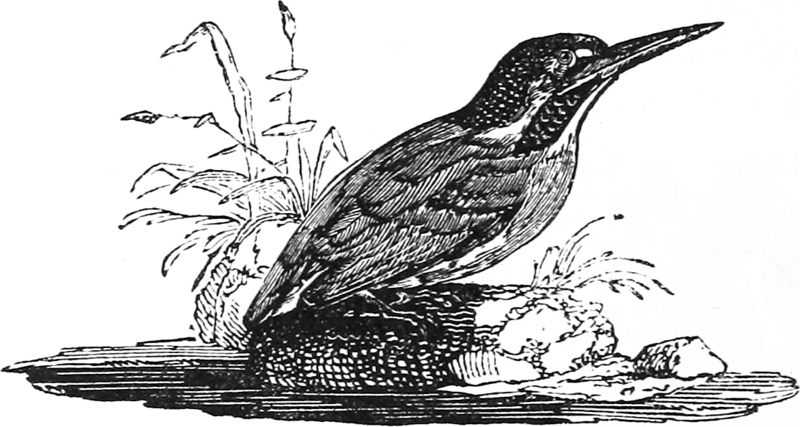
\includegraphics[scale=0.35]{images/Alycon.png}
        \end{figure}
        \vspace{0.5cm}
        \Huge
        \textbf{\textsc{Matematyka Dyskretna}}
        
        \vspace{0.5cm}
        \Large
        \textsc{Wybrane Dowody}
        
        \normalsize
        
        
        \line(1,0){330}
        
        \vspace{1cm}
        \textit{,,Myślę, że 7 punktów na 20 to nie jest zły wynik''}
        \vspace{1cm}

        \textit{\textsc{Popełnione przez}}\\
        \vspace{5mm}

        \textbf{\textsc{Dziurawy Ponton \\ Załatany Ponton \\ Puchaty Pompon \\ Zatopiony Ponton \\ Tonący Ponton \\ Notnop}}

        \vfill

        Kraków \\
        Anno Domini 2023
        
    \end{center}
    
\end{titlepage}


\tableofcontents
\section*{Licencja}
    \begin{figure}[h]
    	\begin{minipage}[c]{0.25\textwidth}
    		
\includegraphics[width=0.7\textwidth]{images/licencja.png}
    	\end{minipage}\hfill
    	\begin{minipage}[c]{0.75\textwidth}
    		\caption*{
    			Ten utwór jest dostępny na 
    			\href{https://creativecommons.org/licenses/by-sa/4.0/}{licencji Creative Commons Uznanie autorstwa
    			na tych samych warunkach 4.0 Międzynarodowe.}
    		}
    	\end{minipage}
    \end{figure}

% Actual content
\mainmatter

\chapter{Kombinatoryka}
 % Żeby nie było syfu to kolejne sekcje dodajemy do chapters/
% A potem includujemy za pomocą \input{chapters/...}

% Używamy \( \) i \[ \] zamiast dolarów -- tak jak się robi w LaTeXu


\documentclass[12pt, a4paper, polish, openany]{book}

% Please, let's familiarize ourselves with notatki.sty and tcs.sty so that we don't reinvent the wheel
\usepackage{notatki}

\fancyhead[L]{\textbf{\textit{MD}}}
\author{
}
\title{TCS and shitposting}


\begin{document}

% Front page and table of contents
\frontmatter

\input{titlepage}

\tableofcontents
\input{license}

% Actual content
\mainmatter

\chapter{Kombinatoryka}
\input{chapters/combinatorics/main}

\chapter{Zasada włączeń i wyłączeń}
\input{chapters/exclusion-inclusion/main}

\chapter{Posety}
\input{chapters/posets/main}

\chapter{Twierdzenie Ramseya}
\input{chapters/ramsey/main}

\chapter{Funkcje tworzące}
\input{chapters/generating_functions/main}

\chapter{Przepływy}
\input{chapters/flows/main}

\chapter{Skojarzenia}
\input{chapters/matchings/main}

\chapter{Kolorowanie grafów}
\input{chapters/graph-coloring/main}

\chapter{Grafy, ale nie kolorowanie}
\input{chapters/graph-misc/main}

\end{document}

\chapter{Zasada włączeń i wyłączeń}
 % Żeby nie było syfu to kolejne sekcje dodajemy do chapters/
% A potem includujemy za pomocą \input{chapters/...}

% Używamy \( \) i \[ \] zamiast dolarów -- tak jak się robi w LaTeXu


\documentclass[12pt, a4paper, polish, openany]{book}

% Please, let's familiarize ourselves with notatki.sty and tcs.sty so that we don't reinvent the wheel
\usepackage{notatki}

\fancyhead[L]{\textbf{\textit{MD}}}
\author{
}
\title{TCS and shitposting}


\begin{document}

% Front page and table of contents
\frontmatter

\input{titlepage}

\tableofcontents
\input{license}

% Actual content
\mainmatter

\chapter{Kombinatoryka}
\input{chapters/combinatorics/main}

\chapter{Zasada włączeń i wyłączeń}
\input{chapters/exclusion-inclusion/main}

\chapter{Posety}
\input{chapters/posets/main}

\chapter{Twierdzenie Ramseya}
\input{chapters/ramsey/main}

\chapter{Funkcje tworzące}
\input{chapters/generating_functions/main}

\chapter{Przepływy}
\input{chapters/flows/main}

\chapter{Skojarzenia}
\input{chapters/matchings/main}

\chapter{Kolorowanie grafów}
\input{chapters/graph-coloring/main}

\chapter{Grafy, ale nie kolorowanie}
\input{chapters/graph-misc/main}

\end{document}

\chapter{Posety}
 % Żeby nie było syfu to kolejne sekcje dodajemy do chapters/
% A potem includujemy za pomocą \input{chapters/...}

% Używamy \( \) i \[ \] zamiast dolarów -- tak jak się robi w LaTeXu


\documentclass[12pt, a4paper, polish, openany]{book}

% Please, let's familiarize ourselves with notatki.sty and tcs.sty so that we don't reinvent the wheel
\usepackage{notatki}

\fancyhead[L]{\textbf{\textit{MD}}}
\author{
}
\title{TCS and shitposting}


\begin{document}

% Front page and table of contents
\frontmatter

\input{titlepage}

\tableofcontents
\input{license}

% Actual content
\mainmatter

\chapter{Kombinatoryka}
\input{chapters/combinatorics/main}

\chapter{Zasada włączeń i wyłączeń}
\input{chapters/exclusion-inclusion/main}

\chapter{Posety}
\input{chapters/posets/main}

\chapter{Twierdzenie Ramseya}
\input{chapters/ramsey/main}

\chapter{Funkcje tworzące}
\input{chapters/generating_functions/main}

\chapter{Przepływy}
\input{chapters/flows/main}

\chapter{Skojarzenia}
\input{chapters/matchings/main}

\chapter{Kolorowanie grafów}
\input{chapters/graph-coloring/main}

\chapter{Grafy, ale nie kolorowanie}
\input{chapters/graph-misc/main}

\end{document}

\chapter{Twierdzenie Ramseya}
 % Żeby nie było syfu to kolejne sekcje dodajemy do chapters/
% A potem includujemy za pomocą \input{chapters/...}

% Używamy \( \) i \[ \] zamiast dolarów -- tak jak się robi w LaTeXu


\documentclass[12pt, a4paper, polish, openany]{book}

% Please, let's familiarize ourselves with notatki.sty and tcs.sty so that we don't reinvent the wheel
\usepackage{notatki}

\fancyhead[L]{\textbf{\textit{MD}}}
\author{
}
\title{TCS and shitposting}


\begin{document}

% Front page and table of contents
\frontmatter

\input{titlepage}

\tableofcontents
\input{license}

% Actual content
\mainmatter

\chapter{Kombinatoryka}
\input{chapters/combinatorics/main}

\chapter{Zasada włączeń i wyłączeń}
\input{chapters/exclusion-inclusion/main}

\chapter{Posety}
\input{chapters/posets/main}

\chapter{Twierdzenie Ramseya}
\input{chapters/ramsey/main}

\chapter{Funkcje tworzące}
\input{chapters/generating_functions/main}

\chapter{Przepływy}
\input{chapters/flows/main}

\chapter{Skojarzenia}
\input{chapters/matchings/main}

\chapter{Kolorowanie grafów}
\input{chapters/graph-coloring/main}

\chapter{Grafy, ale nie kolorowanie}
\input{chapters/graph-misc/main}

\end{document}

\chapter{Funkcje tworzące}
 % Żeby nie było syfu to kolejne sekcje dodajemy do chapters/
% A potem includujemy za pomocą \input{chapters/...}

% Używamy \( \) i \[ \] zamiast dolarów -- tak jak się robi w LaTeXu


\documentclass[12pt, a4paper, polish, openany]{book}

% Please, let's familiarize ourselves with notatki.sty and tcs.sty so that we don't reinvent the wheel
\usepackage{notatki}

\fancyhead[L]{\textbf{\textit{MD}}}
\author{
}
\title{TCS and shitposting}


\begin{document}

% Front page and table of contents
\frontmatter

\input{titlepage}

\tableofcontents
\input{license}

% Actual content
\mainmatter

\chapter{Kombinatoryka}
\input{chapters/combinatorics/main}

\chapter{Zasada włączeń i wyłączeń}
\input{chapters/exclusion-inclusion/main}

\chapter{Posety}
\input{chapters/posets/main}

\chapter{Twierdzenie Ramseya}
\input{chapters/ramsey/main}

\chapter{Funkcje tworzące}
\input{chapters/generating_functions/main}

\chapter{Przepływy}
\input{chapters/flows/main}

\chapter{Skojarzenia}
\input{chapters/matchings/main}

\chapter{Kolorowanie grafów}
\input{chapters/graph-coloring/main}

\chapter{Grafy, ale nie kolorowanie}
\input{chapters/graph-misc/main}

\end{document}

\chapter{Przepływy}
 % Żeby nie było syfu to kolejne sekcje dodajemy do chapters/
% A potem includujemy za pomocą \input{chapters/...}

% Używamy \( \) i \[ \] zamiast dolarów -- tak jak się robi w LaTeXu


\documentclass[12pt, a4paper, polish, openany]{book}

% Please, let's familiarize ourselves with notatki.sty and tcs.sty so that we don't reinvent the wheel
\usepackage{notatki}

\fancyhead[L]{\textbf{\textit{MD}}}
\author{
}
\title{TCS and shitposting}


\begin{document}

% Front page and table of contents
\frontmatter

\input{titlepage}

\tableofcontents
\input{license}

% Actual content
\mainmatter

\chapter{Kombinatoryka}
\input{chapters/combinatorics/main}

\chapter{Zasada włączeń i wyłączeń}
\input{chapters/exclusion-inclusion/main}

\chapter{Posety}
\input{chapters/posets/main}

\chapter{Twierdzenie Ramseya}
\input{chapters/ramsey/main}

\chapter{Funkcje tworzące}
\input{chapters/generating_functions/main}

\chapter{Przepływy}
\input{chapters/flows/main}

\chapter{Skojarzenia}
\input{chapters/matchings/main}

\chapter{Kolorowanie grafów}
\input{chapters/graph-coloring/main}

\chapter{Grafy, ale nie kolorowanie}
\input{chapters/graph-misc/main}

\end{document}

\chapter{Skojarzenia}
 % Żeby nie było syfu to kolejne sekcje dodajemy do chapters/
% A potem includujemy za pomocą \input{chapters/...}

% Używamy \( \) i \[ \] zamiast dolarów -- tak jak się robi w LaTeXu


\documentclass[12pt, a4paper, polish, openany]{book}

% Please, let's familiarize ourselves with notatki.sty and tcs.sty so that we don't reinvent the wheel
\usepackage{notatki}

\fancyhead[L]{\textbf{\textit{MD}}}
\author{
}
\title{TCS and shitposting}


\begin{document}

% Front page and table of contents
\frontmatter

\input{titlepage}

\tableofcontents
\input{license}

% Actual content
\mainmatter

\chapter{Kombinatoryka}
\input{chapters/combinatorics/main}

\chapter{Zasada włączeń i wyłączeń}
\input{chapters/exclusion-inclusion/main}

\chapter{Posety}
\input{chapters/posets/main}

\chapter{Twierdzenie Ramseya}
\input{chapters/ramsey/main}

\chapter{Funkcje tworzące}
\input{chapters/generating_functions/main}

\chapter{Przepływy}
\input{chapters/flows/main}

\chapter{Skojarzenia}
\input{chapters/matchings/main}

\chapter{Kolorowanie grafów}
\input{chapters/graph-coloring/main}

\chapter{Grafy, ale nie kolorowanie}
\input{chapters/graph-misc/main}

\end{document}

\chapter{Kolorowanie grafów}
 % Żeby nie było syfu to kolejne sekcje dodajemy do chapters/
% A potem includujemy za pomocą \input{chapters/...}

% Używamy \( \) i \[ \] zamiast dolarów -- tak jak się robi w LaTeXu


\documentclass[12pt, a4paper, polish, openany]{book}

% Please, let's familiarize ourselves with notatki.sty and tcs.sty so that we don't reinvent the wheel
\usepackage{notatki}

\fancyhead[L]{\textbf{\textit{MD}}}
\author{
}
\title{TCS and shitposting}


\begin{document}

% Front page and table of contents
\frontmatter

\input{titlepage}

\tableofcontents
\input{license}

% Actual content
\mainmatter

\chapter{Kombinatoryka}
\input{chapters/combinatorics/main}

\chapter{Zasada włączeń i wyłączeń}
\input{chapters/exclusion-inclusion/main}

\chapter{Posety}
\input{chapters/posets/main}

\chapter{Twierdzenie Ramseya}
\input{chapters/ramsey/main}

\chapter{Funkcje tworzące}
\input{chapters/generating_functions/main}

\chapter{Przepływy}
\input{chapters/flows/main}

\chapter{Skojarzenia}
\input{chapters/matchings/main}

\chapter{Kolorowanie grafów}
\input{chapters/graph-coloring/main}

\chapter{Grafy, ale nie kolorowanie}
\input{chapters/graph-misc/main}

\end{document}

\chapter{Grafy, ale nie kolorowanie}
 % Żeby nie było syfu to kolejne sekcje dodajemy do chapters/
% A potem includujemy za pomocą \input{chapters/...}

% Używamy \( \) i \[ \] zamiast dolarów -- tak jak się robi w LaTeXu


\documentclass[12pt, a4paper, polish, openany]{book}

% Please, let's familiarize ourselves with notatki.sty and tcs.sty so that we don't reinvent the wheel
\usepackage{notatki}

\fancyhead[L]{\textbf{\textit{MD}}}
\author{
}
\title{TCS and shitposting}


\begin{document}

% Front page and table of contents
\frontmatter

\input{titlepage}

\tableofcontents
\input{license}

% Actual content
\mainmatter

\chapter{Kombinatoryka}
\input{chapters/combinatorics/main}

\chapter{Zasada włączeń i wyłączeń}
\input{chapters/exclusion-inclusion/main}

\chapter{Posety}
\input{chapters/posets/main}

\chapter{Twierdzenie Ramseya}
\input{chapters/ramsey/main}

\chapter{Funkcje tworzące}
\input{chapters/generating_functions/main}

\chapter{Przepływy}
\input{chapters/flows/main}

\chapter{Skojarzenia}
\input{chapters/matchings/main}

\chapter{Kolorowanie grafów}
\input{chapters/graph-coloring/main}

\chapter{Grafy, ale nie kolorowanie}
\input{chapters/graph-misc/main}

\end{document}

\end{document}

\chapter{Skojarzenia}
 % Żeby nie było syfu to kolejne sekcje dodajemy do chapters/
% A potem includujemy za pomocą \input{chapters/...}

% Używamy \( \) i \[ \] zamiast dolarów -- tak jak się robi w LaTeXu


\documentclass[12pt, a4paper, polish, openany]{book}

% Please, let's familiarize ourselves with notatki.sty and tcs.sty so that we don't reinvent the wheel
\usepackage{notatki}

\fancyhead[L]{\textbf{\textit{MD}}}
\author{
}
\title{TCS and shitposting}


\begin{document}

% Front page and table of contents
\frontmatter

\begin{titlepage} 

    \begin{center}
         \begin{figure}[h]
            \centering
            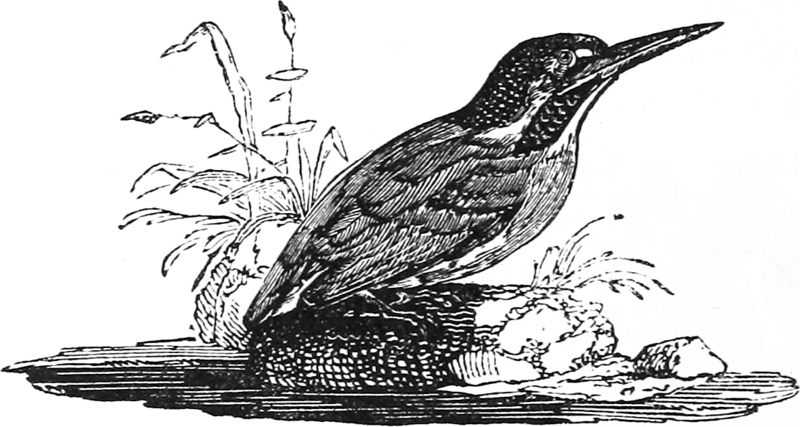
\includegraphics[scale=0.35]{images/Alycon.png}
        \end{figure}
        \vspace{0.5cm}
        \Huge
        \textbf{\textsc{Matematyka Dyskretna}}
        
        \vspace{0.5cm}
        \Large
        \textsc{Wybrane Dowody}
        
        \normalsize
        
        
        \line(1,0){330}
        
        \vspace{1cm}
        \textit{,,Myślę, że 7 punktów na 20 to nie jest zły wynik''}
        \vspace{1cm}

        \textit{\textsc{Popełnione przez}}\\
        \vspace{5mm}

        \textbf{\textsc{Dziurawy Ponton \\ Załatany Ponton \\ Puchaty Pompon \\ Zatopiony Ponton \\ Tonący Ponton \\ Notnop}}

        \vfill

        Kraków \\
        Anno Domini 2023
        
    \end{center}
    
\end{titlepage}


\tableofcontents
\section*{Licencja}
    \begin{figure}[h]
    	\begin{minipage}[c]{0.25\textwidth}
    		
\includegraphics[width=0.7\textwidth]{images/licencja.png}
    	\end{minipage}\hfill
    	\begin{minipage}[c]{0.75\textwidth}
    		\caption*{
    			Ten utwór jest dostępny na 
    			\href{https://creativecommons.org/licenses/by-sa/4.0/}{licencji Creative Commons Uznanie autorstwa
    			na tych samych warunkach 4.0 Międzynarodowe.}
    		}
    	\end{minipage}
    \end{figure}

% Actual content
\mainmatter

\chapter{Kombinatoryka}
 % Żeby nie było syfu to kolejne sekcje dodajemy do chapters/
% A potem includujemy za pomocą \input{chapters/...}

% Używamy \( \) i \[ \] zamiast dolarów -- tak jak się robi w LaTeXu


\documentclass[12pt, a4paper, polish, openany]{book}

% Please, let's familiarize ourselves with notatki.sty and tcs.sty so that we don't reinvent the wheel
\usepackage{notatki}

\fancyhead[L]{\textbf{\textit{MD}}}
\author{
}
\title{TCS and shitposting}


\begin{document}

% Front page and table of contents
\frontmatter

\input{titlepage}

\tableofcontents
\input{license}

% Actual content
\mainmatter

\chapter{Kombinatoryka}
\input{chapters/combinatorics/main}

\chapter{Zasada włączeń i wyłączeń}
\input{chapters/exclusion-inclusion/main}

\chapter{Posety}
\input{chapters/posets/main}

\chapter{Twierdzenie Ramseya}
\input{chapters/ramsey/main}

\chapter{Funkcje tworzące}
\input{chapters/generating_functions/main}

\chapter{Przepływy}
\input{chapters/flows/main}

\chapter{Skojarzenia}
\input{chapters/matchings/main}

\chapter{Kolorowanie grafów}
\input{chapters/graph-coloring/main}

\chapter{Grafy, ale nie kolorowanie}
\input{chapters/graph-misc/main}

\end{document}

\chapter{Zasada włączeń i wyłączeń}
 % Żeby nie było syfu to kolejne sekcje dodajemy do chapters/
% A potem includujemy za pomocą \input{chapters/...}

% Używamy \( \) i \[ \] zamiast dolarów -- tak jak się robi w LaTeXu


\documentclass[12pt, a4paper, polish, openany]{book}

% Please, let's familiarize ourselves with notatki.sty and tcs.sty so that we don't reinvent the wheel
\usepackage{notatki}

\fancyhead[L]{\textbf{\textit{MD}}}
\author{
}
\title{TCS and shitposting}


\begin{document}

% Front page and table of contents
\frontmatter

\input{titlepage}

\tableofcontents
\input{license}

% Actual content
\mainmatter

\chapter{Kombinatoryka}
\input{chapters/combinatorics/main}

\chapter{Zasada włączeń i wyłączeń}
\input{chapters/exclusion-inclusion/main}

\chapter{Posety}
\input{chapters/posets/main}

\chapter{Twierdzenie Ramseya}
\input{chapters/ramsey/main}

\chapter{Funkcje tworzące}
\input{chapters/generating_functions/main}

\chapter{Przepływy}
\input{chapters/flows/main}

\chapter{Skojarzenia}
\input{chapters/matchings/main}

\chapter{Kolorowanie grafów}
\input{chapters/graph-coloring/main}

\chapter{Grafy, ale nie kolorowanie}
\input{chapters/graph-misc/main}

\end{document}

\chapter{Posety}
 % Żeby nie było syfu to kolejne sekcje dodajemy do chapters/
% A potem includujemy za pomocą \input{chapters/...}

% Używamy \( \) i \[ \] zamiast dolarów -- tak jak się robi w LaTeXu


\documentclass[12pt, a4paper, polish, openany]{book}

% Please, let's familiarize ourselves with notatki.sty and tcs.sty so that we don't reinvent the wheel
\usepackage{notatki}

\fancyhead[L]{\textbf{\textit{MD}}}
\author{
}
\title{TCS and shitposting}


\begin{document}

% Front page and table of contents
\frontmatter

\input{titlepage}

\tableofcontents
\input{license}

% Actual content
\mainmatter

\chapter{Kombinatoryka}
\input{chapters/combinatorics/main}

\chapter{Zasada włączeń i wyłączeń}
\input{chapters/exclusion-inclusion/main}

\chapter{Posety}
\input{chapters/posets/main}

\chapter{Twierdzenie Ramseya}
\input{chapters/ramsey/main}

\chapter{Funkcje tworzące}
\input{chapters/generating_functions/main}

\chapter{Przepływy}
\input{chapters/flows/main}

\chapter{Skojarzenia}
\input{chapters/matchings/main}

\chapter{Kolorowanie grafów}
\input{chapters/graph-coloring/main}

\chapter{Grafy, ale nie kolorowanie}
\input{chapters/graph-misc/main}

\end{document}

\chapter{Twierdzenie Ramseya}
 % Żeby nie było syfu to kolejne sekcje dodajemy do chapters/
% A potem includujemy za pomocą \input{chapters/...}

% Używamy \( \) i \[ \] zamiast dolarów -- tak jak się robi w LaTeXu


\documentclass[12pt, a4paper, polish, openany]{book}

% Please, let's familiarize ourselves with notatki.sty and tcs.sty so that we don't reinvent the wheel
\usepackage{notatki}

\fancyhead[L]{\textbf{\textit{MD}}}
\author{
}
\title{TCS and shitposting}


\begin{document}

% Front page and table of contents
\frontmatter

\input{titlepage}

\tableofcontents
\input{license}

% Actual content
\mainmatter

\chapter{Kombinatoryka}
\input{chapters/combinatorics/main}

\chapter{Zasada włączeń i wyłączeń}
\input{chapters/exclusion-inclusion/main}

\chapter{Posety}
\input{chapters/posets/main}

\chapter{Twierdzenie Ramseya}
\input{chapters/ramsey/main}

\chapter{Funkcje tworzące}
\input{chapters/generating_functions/main}

\chapter{Przepływy}
\input{chapters/flows/main}

\chapter{Skojarzenia}
\input{chapters/matchings/main}

\chapter{Kolorowanie grafów}
\input{chapters/graph-coloring/main}

\chapter{Grafy, ale nie kolorowanie}
\input{chapters/graph-misc/main}

\end{document}

\chapter{Funkcje tworzące}
 % Żeby nie było syfu to kolejne sekcje dodajemy do chapters/
% A potem includujemy za pomocą \input{chapters/...}

% Używamy \( \) i \[ \] zamiast dolarów -- tak jak się robi w LaTeXu


\documentclass[12pt, a4paper, polish, openany]{book}

% Please, let's familiarize ourselves with notatki.sty and tcs.sty so that we don't reinvent the wheel
\usepackage{notatki}

\fancyhead[L]{\textbf{\textit{MD}}}
\author{
}
\title{TCS and shitposting}


\begin{document}

% Front page and table of contents
\frontmatter

\input{titlepage}

\tableofcontents
\input{license}

% Actual content
\mainmatter

\chapter{Kombinatoryka}
\input{chapters/combinatorics/main}

\chapter{Zasada włączeń i wyłączeń}
\input{chapters/exclusion-inclusion/main}

\chapter{Posety}
\input{chapters/posets/main}

\chapter{Twierdzenie Ramseya}
\input{chapters/ramsey/main}

\chapter{Funkcje tworzące}
\input{chapters/generating_functions/main}

\chapter{Przepływy}
\input{chapters/flows/main}

\chapter{Skojarzenia}
\input{chapters/matchings/main}

\chapter{Kolorowanie grafów}
\input{chapters/graph-coloring/main}

\chapter{Grafy, ale nie kolorowanie}
\input{chapters/graph-misc/main}

\end{document}

\chapter{Przepływy}
 % Żeby nie było syfu to kolejne sekcje dodajemy do chapters/
% A potem includujemy za pomocą \input{chapters/...}

% Używamy \( \) i \[ \] zamiast dolarów -- tak jak się robi w LaTeXu


\documentclass[12pt, a4paper, polish, openany]{book}

% Please, let's familiarize ourselves with notatki.sty and tcs.sty so that we don't reinvent the wheel
\usepackage{notatki}

\fancyhead[L]{\textbf{\textit{MD}}}
\author{
}
\title{TCS and shitposting}


\begin{document}

% Front page and table of contents
\frontmatter

\input{titlepage}

\tableofcontents
\input{license}

% Actual content
\mainmatter

\chapter{Kombinatoryka}
\input{chapters/combinatorics/main}

\chapter{Zasada włączeń i wyłączeń}
\input{chapters/exclusion-inclusion/main}

\chapter{Posety}
\input{chapters/posets/main}

\chapter{Twierdzenie Ramseya}
\input{chapters/ramsey/main}

\chapter{Funkcje tworzące}
\input{chapters/generating_functions/main}

\chapter{Przepływy}
\input{chapters/flows/main}

\chapter{Skojarzenia}
\input{chapters/matchings/main}

\chapter{Kolorowanie grafów}
\input{chapters/graph-coloring/main}

\chapter{Grafy, ale nie kolorowanie}
\input{chapters/graph-misc/main}

\end{document}

\chapter{Skojarzenia}
 % Żeby nie było syfu to kolejne sekcje dodajemy do chapters/
% A potem includujemy za pomocą \input{chapters/...}

% Używamy \( \) i \[ \] zamiast dolarów -- tak jak się robi w LaTeXu


\documentclass[12pt, a4paper, polish, openany]{book}

% Please, let's familiarize ourselves with notatki.sty and tcs.sty so that we don't reinvent the wheel
\usepackage{notatki}

\fancyhead[L]{\textbf{\textit{MD}}}
\author{
}
\title{TCS and shitposting}


\begin{document}

% Front page and table of contents
\frontmatter

\input{titlepage}

\tableofcontents
\input{license}

% Actual content
\mainmatter

\chapter{Kombinatoryka}
\input{chapters/combinatorics/main}

\chapter{Zasada włączeń i wyłączeń}
\input{chapters/exclusion-inclusion/main}

\chapter{Posety}
\input{chapters/posets/main}

\chapter{Twierdzenie Ramseya}
\input{chapters/ramsey/main}

\chapter{Funkcje tworzące}
\input{chapters/generating_functions/main}

\chapter{Przepływy}
\input{chapters/flows/main}

\chapter{Skojarzenia}
\input{chapters/matchings/main}

\chapter{Kolorowanie grafów}
\input{chapters/graph-coloring/main}

\chapter{Grafy, ale nie kolorowanie}
\input{chapters/graph-misc/main}

\end{document}

\chapter{Kolorowanie grafów}
 % Żeby nie było syfu to kolejne sekcje dodajemy do chapters/
% A potem includujemy za pomocą \input{chapters/...}

% Używamy \( \) i \[ \] zamiast dolarów -- tak jak się robi w LaTeXu


\documentclass[12pt, a4paper, polish, openany]{book}

% Please, let's familiarize ourselves with notatki.sty and tcs.sty so that we don't reinvent the wheel
\usepackage{notatki}

\fancyhead[L]{\textbf{\textit{MD}}}
\author{
}
\title{TCS and shitposting}


\begin{document}

% Front page and table of contents
\frontmatter

\input{titlepage}

\tableofcontents
\input{license}

% Actual content
\mainmatter

\chapter{Kombinatoryka}
\input{chapters/combinatorics/main}

\chapter{Zasada włączeń i wyłączeń}
\input{chapters/exclusion-inclusion/main}

\chapter{Posety}
\input{chapters/posets/main}

\chapter{Twierdzenie Ramseya}
\input{chapters/ramsey/main}

\chapter{Funkcje tworzące}
\input{chapters/generating_functions/main}

\chapter{Przepływy}
\input{chapters/flows/main}

\chapter{Skojarzenia}
\input{chapters/matchings/main}

\chapter{Kolorowanie grafów}
\input{chapters/graph-coloring/main}

\chapter{Grafy, ale nie kolorowanie}
\input{chapters/graph-misc/main}

\end{document}

\chapter{Grafy, ale nie kolorowanie}
 % Żeby nie było syfu to kolejne sekcje dodajemy do chapters/
% A potem includujemy za pomocą \input{chapters/...}

% Używamy \( \) i \[ \] zamiast dolarów -- tak jak się robi w LaTeXu


\documentclass[12pt, a4paper, polish, openany]{book}

% Please, let's familiarize ourselves with notatki.sty and tcs.sty so that we don't reinvent the wheel
\usepackage{notatki}

\fancyhead[L]{\textbf{\textit{MD}}}
\author{
}
\title{TCS and shitposting}


\begin{document}

% Front page and table of contents
\frontmatter

\input{titlepage}

\tableofcontents
\input{license}

% Actual content
\mainmatter

\chapter{Kombinatoryka}
\input{chapters/combinatorics/main}

\chapter{Zasada włączeń i wyłączeń}
\input{chapters/exclusion-inclusion/main}

\chapter{Posety}
\input{chapters/posets/main}

\chapter{Twierdzenie Ramseya}
\input{chapters/ramsey/main}

\chapter{Funkcje tworzące}
\input{chapters/generating_functions/main}

\chapter{Przepływy}
\input{chapters/flows/main}

\chapter{Skojarzenia}
\input{chapters/matchings/main}

\chapter{Kolorowanie grafów}
\input{chapters/graph-coloring/main}

\chapter{Grafy, ale nie kolorowanie}
\input{chapters/graph-misc/main}

\end{document}

\end{document}

\chapter{Kolorowanie grafów}
 % Żeby nie było syfu to kolejne sekcje dodajemy do chapters/
% A potem includujemy za pomocą \input{chapters/...}

% Używamy \( \) i \[ \] zamiast dolarów -- tak jak się robi w LaTeXu


\documentclass[12pt, a4paper, polish, openany]{book}

% Please, let's familiarize ourselves with notatki.sty and tcs.sty so that we don't reinvent the wheel
\usepackage{notatki}

\fancyhead[L]{\textbf{\textit{MD}}}
\author{
}
\title{TCS and shitposting}


\begin{document}

% Front page and table of contents
\frontmatter

\begin{titlepage} 

    \begin{center}
         \begin{figure}[h]
            \centering
            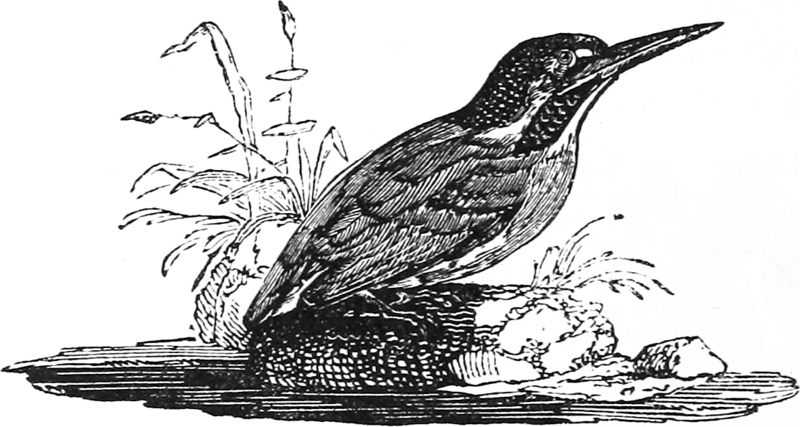
\includegraphics[scale=0.35]{images/Alycon.png}
        \end{figure}
        \vspace{0.5cm}
        \Huge
        \textbf{\textsc{Matematyka Dyskretna}}
        
        \vspace{0.5cm}
        \Large
        \textsc{Wybrane Dowody}
        
        \normalsize
        
        
        \line(1,0){330}
        
        \vspace{1cm}
        \textit{,,Myślę, że 7 punktów na 20 to nie jest zły wynik''}
        \vspace{1cm}

        \textit{\textsc{Popełnione przez}}\\
        \vspace{5mm}

        \textbf{\textsc{Dziurawy Ponton \\ Załatany Ponton \\ Puchaty Pompon \\ Zatopiony Ponton \\ Tonący Ponton \\ Notnop}}

        \vfill

        Kraków \\
        Anno Domini 2023
        
    \end{center}
    
\end{titlepage}


\tableofcontents
\section*{Licencja}
    \begin{figure}[h]
    	\begin{minipage}[c]{0.25\textwidth}
    		
\includegraphics[width=0.7\textwidth]{images/licencja.png}
    	\end{minipage}\hfill
    	\begin{minipage}[c]{0.75\textwidth}
    		\caption*{
    			Ten utwór jest dostępny na 
    			\href{https://creativecommons.org/licenses/by-sa/4.0/}{licencji Creative Commons Uznanie autorstwa
    			na tych samych warunkach 4.0 Międzynarodowe.}
    		}
    	\end{minipage}
    \end{figure}

% Actual content
\mainmatter

\chapter{Kombinatoryka}
 % Żeby nie było syfu to kolejne sekcje dodajemy do chapters/
% A potem includujemy za pomocą \input{chapters/...}

% Używamy \( \) i \[ \] zamiast dolarów -- tak jak się robi w LaTeXu


\documentclass[12pt, a4paper, polish, openany]{book}

% Please, let's familiarize ourselves with notatki.sty and tcs.sty so that we don't reinvent the wheel
\usepackage{notatki}

\fancyhead[L]{\textbf{\textit{MD}}}
\author{
}
\title{TCS and shitposting}


\begin{document}

% Front page and table of contents
\frontmatter

\input{titlepage}

\tableofcontents
\input{license}

% Actual content
\mainmatter

\chapter{Kombinatoryka}
\input{chapters/combinatorics/main}

\chapter{Zasada włączeń i wyłączeń}
\input{chapters/exclusion-inclusion/main}

\chapter{Posety}
\input{chapters/posets/main}

\chapter{Twierdzenie Ramseya}
\input{chapters/ramsey/main}

\chapter{Funkcje tworzące}
\input{chapters/generating_functions/main}

\chapter{Przepływy}
\input{chapters/flows/main}

\chapter{Skojarzenia}
\input{chapters/matchings/main}

\chapter{Kolorowanie grafów}
\input{chapters/graph-coloring/main}

\chapter{Grafy, ale nie kolorowanie}
\input{chapters/graph-misc/main}

\end{document}

\chapter{Zasada włączeń i wyłączeń}
 % Żeby nie było syfu to kolejne sekcje dodajemy do chapters/
% A potem includujemy za pomocą \input{chapters/...}

% Używamy \( \) i \[ \] zamiast dolarów -- tak jak się robi w LaTeXu


\documentclass[12pt, a4paper, polish, openany]{book}

% Please, let's familiarize ourselves with notatki.sty and tcs.sty so that we don't reinvent the wheel
\usepackage{notatki}

\fancyhead[L]{\textbf{\textit{MD}}}
\author{
}
\title{TCS and shitposting}


\begin{document}

% Front page and table of contents
\frontmatter

\input{titlepage}

\tableofcontents
\input{license}

% Actual content
\mainmatter

\chapter{Kombinatoryka}
\input{chapters/combinatorics/main}

\chapter{Zasada włączeń i wyłączeń}
\input{chapters/exclusion-inclusion/main}

\chapter{Posety}
\input{chapters/posets/main}

\chapter{Twierdzenie Ramseya}
\input{chapters/ramsey/main}

\chapter{Funkcje tworzące}
\input{chapters/generating_functions/main}

\chapter{Przepływy}
\input{chapters/flows/main}

\chapter{Skojarzenia}
\input{chapters/matchings/main}

\chapter{Kolorowanie grafów}
\input{chapters/graph-coloring/main}

\chapter{Grafy, ale nie kolorowanie}
\input{chapters/graph-misc/main}

\end{document}

\chapter{Posety}
 % Żeby nie było syfu to kolejne sekcje dodajemy do chapters/
% A potem includujemy za pomocą \input{chapters/...}

% Używamy \( \) i \[ \] zamiast dolarów -- tak jak się robi w LaTeXu


\documentclass[12pt, a4paper, polish, openany]{book}

% Please, let's familiarize ourselves with notatki.sty and tcs.sty so that we don't reinvent the wheel
\usepackage{notatki}

\fancyhead[L]{\textbf{\textit{MD}}}
\author{
}
\title{TCS and shitposting}


\begin{document}

% Front page and table of contents
\frontmatter

\input{titlepage}

\tableofcontents
\input{license}

% Actual content
\mainmatter

\chapter{Kombinatoryka}
\input{chapters/combinatorics/main}

\chapter{Zasada włączeń i wyłączeń}
\input{chapters/exclusion-inclusion/main}

\chapter{Posety}
\input{chapters/posets/main}

\chapter{Twierdzenie Ramseya}
\input{chapters/ramsey/main}

\chapter{Funkcje tworzące}
\input{chapters/generating_functions/main}

\chapter{Przepływy}
\input{chapters/flows/main}

\chapter{Skojarzenia}
\input{chapters/matchings/main}

\chapter{Kolorowanie grafów}
\input{chapters/graph-coloring/main}

\chapter{Grafy, ale nie kolorowanie}
\input{chapters/graph-misc/main}

\end{document}

\chapter{Twierdzenie Ramseya}
 % Żeby nie było syfu to kolejne sekcje dodajemy do chapters/
% A potem includujemy za pomocą \input{chapters/...}

% Używamy \( \) i \[ \] zamiast dolarów -- tak jak się robi w LaTeXu


\documentclass[12pt, a4paper, polish, openany]{book}

% Please, let's familiarize ourselves with notatki.sty and tcs.sty so that we don't reinvent the wheel
\usepackage{notatki}

\fancyhead[L]{\textbf{\textit{MD}}}
\author{
}
\title{TCS and shitposting}


\begin{document}

% Front page and table of contents
\frontmatter

\input{titlepage}

\tableofcontents
\input{license}

% Actual content
\mainmatter

\chapter{Kombinatoryka}
\input{chapters/combinatorics/main}

\chapter{Zasada włączeń i wyłączeń}
\input{chapters/exclusion-inclusion/main}

\chapter{Posety}
\input{chapters/posets/main}

\chapter{Twierdzenie Ramseya}
\input{chapters/ramsey/main}

\chapter{Funkcje tworzące}
\input{chapters/generating_functions/main}

\chapter{Przepływy}
\input{chapters/flows/main}

\chapter{Skojarzenia}
\input{chapters/matchings/main}

\chapter{Kolorowanie grafów}
\input{chapters/graph-coloring/main}

\chapter{Grafy, ale nie kolorowanie}
\input{chapters/graph-misc/main}

\end{document}

\chapter{Funkcje tworzące}
 % Żeby nie było syfu to kolejne sekcje dodajemy do chapters/
% A potem includujemy za pomocą \input{chapters/...}

% Używamy \( \) i \[ \] zamiast dolarów -- tak jak się robi w LaTeXu


\documentclass[12pt, a4paper, polish, openany]{book}

% Please, let's familiarize ourselves with notatki.sty and tcs.sty so that we don't reinvent the wheel
\usepackage{notatki}

\fancyhead[L]{\textbf{\textit{MD}}}
\author{
}
\title{TCS and shitposting}


\begin{document}

% Front page and table of contents
\frontmatter

\input{titlepage}

\tableofcontents
\input{license}

% Actual content
\mainmatter

\chapter{Kombinatoryka}
\input{chapters/combinatorics/main}

\chapter{Zasada włączeń i wyłączeń}
\input{chapters/exclusion-inclusion/main}

\chapter{Posety}
\input{chapters/posets/main}

\chapter{Twierdzenie Ramseya}
\input{chapters/ramsey/main}

\chapter{Funkcje tworzące}
\input{chapters/generating_functions/main}

\chapter{Przepływy}
\input{chapters/flows/main}

\chapter{Skojarzenia}
\input{chapters/matchings/main}

\chapter{Kolorowanie grafów}
\input{chapters/graph-coloring/main}

\chapter{Grafy, ale nie kolorowanie}
\input{chapters/graph-misc/main}

\end{document}

\chapter{Przepływy}
 % Żeby nie było syfu to kolejne sekcje dodajemy do chapters/
% A potem includujemy za pomocą \input{chapters/...}

% Używamy \( \) i \[ \] zamiast dolarów -- tak jak się robi w LaTeXu


\documentclass[12pt, a4paper, polish, openany]{book}

% Please, let's familiarize ourselves with notatki.sty and tcs.sty so that we don't reinvent the wheel
\usepackage{notatki}

\fancyhead[L]{\textbf{\textit{MD}}}
\author{
}
\title{TCS and shitposting}


\begin{document}

% Front page and table of contents
\frontmatter

\input{titlepage}

\tableofcontents
\input{license}

% Actual content
\mainmatter

\chapter{Kombinatoryka}
\input{chapters/combinatorics/main}

\chapter{Zasada włączeń i wyłączeń}
\input{chapters/exclusion-inclusion/main}

\chapter{Posety}
\input{chapters/posets/main}

\chapter{Twierdzenie Ramseya}
\input{chapters/ramsey/main}

\chapter{Funkcje tworzące}
\input{chapters/generating_functions/main}

\chapter{Przepływy}
\input{chapters/flows/main}

\chapter{Skojarzenia}
\input{chapters/matchings/main}

\chapter{Kolorowanie grafów}
\input{chapters/graph-coloring/main}

\chapter{Grafy, ale nie kolorowanie}
\input{chapters/graph-misc/main}

\end{document}

\chapter{Skojarzenia}
 % Żeby nie było syfu to kolejne sekcje dodajemy do chapters/
% A potem includujemy za pomocą \input{chapters/...}

% Używamy \( \) i \[ \] zamiast dolarów -- tak jak się robi w LaTeXu


\documentclass[12pt, a4paper, polish, openany]{book}

% Please, let's familiarize ourselves with notatki.sty and tcs.sty so that we don't reinvent the wheel
\usepackage{notatki}

\fancyhead[L]{\textbf{\textit{MD}}}
\author{
}
\title{TCS and shitposting}


\begin{document}

% Front page and table of contents
\frontmatter

\input{titlepage}

\tableofcontents
\input{license}

% Actual content
\mainmatter

\chapter{Kombinatoryka}
\input{chapters/combinatorics/main}

\chapter{Zasada włączeń i wyłączeń}
\input{chapters/exclusion-inclusion/main}

\chapter{Posety}
\input{chapters/posets/main}

\chapter{Twierdzenie Ramseya}
\input{chapters/ramsey/main}

\chapter{Funkcje tworzące}
\input{chapters/generating_functions/main}

\chapter{Przepływy}
\input{chapters/flows/main}

\chapter{Skojarzenia}
\input{chapters/matchings/main}

\chapter{Kolorowanie grafów}
\input{chapters/graph-coloring/main}

\chapter{Grafy, ale nie kolorowanie}
\input{chapters/graph-misc/main}

\end{document}

\chapter{Kolorowanie grafów}
 % Żeby nie było syfu to kolejne sekcje dodajemy do chapters/
% A potem includujemy za pomocą \input{chapters/...}

% Używamy \( \) i \[ \] zamiast dolarów -- tak jak się robi w LaTeXu


\documentclass[12pt, a4paper, polish, openany]{book}

% Please, let's familiarize ourselves with notatki.sty and tcs.sty so that we don't reinvent the wheel
\usepackage{notatki}

\fancyhead[L]{\textbf{\textit{MD}}}
\author{
}
\title{TCS and shitposting}


\begin{document}

% Front page and table of contents
\frontmatter

\input{titlepage}

\tableofcontents
\input{license}

% Actual content
\mainmatter

\chapter{Kombinatoryka}
\input{chapters/combinatorics/main}

\chapter{Zasada włączeń i wyłączeń}
\input{chapters/exclusion-inclusion/main}

\chapter{Posety}
\input{chapters/posets/main}

\chapter{Twierdzenie Ramseya}
\input{chapters/ramsey/main}

\chapter{Funkcje tworzące}
\input{chapters/generating_functions/main}

\chapter{Przepływy}
\input{chapters/flows/main}

\chapter{Skojarzenia}
\input{chapters/matchings/main}

\chapter{Kolorowanie grafów}
\input{chapters/graph-coloring/main}

\chapter{Grafy, ale nie kolorowanie}
\input{chapters/graph-misc/main}

\end{document}

\chapter{Grafy, ale nie kolorowanie}
 % Żeby nie było syfu to kolejne sekcje dodajemy do chapters/
% A potem includujemy za pomocą \input{chapters/...}

% Używamy \( \) i \[ \] zamiast dolarów -- tak jak się robi w LaTeXu


\documentclass[12pt, a4paper, polish, openany]{book}

% Please, let's familiarize ourselves with notatki.sty and tcs.sty so that we don't reinvent the wheel
\usepackage{notatki}

\fancyhead[L]{\textbf{\textit{MD}}}
\author{
}
\title{TCS and shitposting}


\begin{document}

% Front page and table of contents
\frontmatter

\input{titlepage}

\tableofcontents
\input{license}

% Actual content
\mainmatter

\chapter{Kombinatoryka}
\input{chapters/combinatorics/main}

\chapter{Zasada włączeń i wyłączeń}
\input{chapters/exclusion-inclusion/main}

\chapter{Posety}
\input{chapters/posets/main}

\chapter{Twierdzenie Ramseya}
\input{chapters/ramsey/main}

\chapter{Funkcje tworzące}
\input{chapters/generating_functions/main}

\chapter{Przepływy}
\input{chapters/flows/main}

\chapter{Skojarzenia}
\input{chapters/matchings/main}

\chapter{Kolorowanie grafów}
\input{chapters/graph-coloring/main}

\chapter{Grafy, ale nie kolorowanie}
\input{chapters/graph-misc/main}

\end{document}

\end{document}

\chapter{Grafy, ale nie kolorowanie}
 % Żeby nie było syfu to kolejne sekcje dodajemy do chapters/
% A potem includujemy za pomocą \input{chapters/...}

% Używamy \( \) i \[ \] zamiast dolarów -- tak jak się robi w LaTeXu


\documentclass[12pt, a4paper, polish, openany]{book}

% Please, let's familiarize ourselves with notatki.sty and tcs.sty so that we don't reinvent the wheel
\usepackage{notatki}

\fancyhead[L]{\textbf{\textit{MD}}}
\author{
}
\title{TCS and shitposting}


\begin{document}

% Front page and table of contents
\frontmatter

\begin{titlepage} 

    \begin{center}
         \begin{figure}[h]
            \centering
            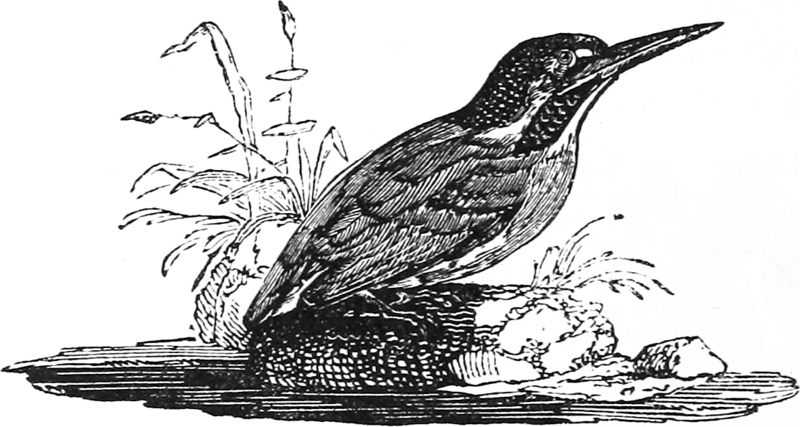
\includegraphics[scale=0.35]{images/Alycon.png}
        \end{figure}
        \vspace{0.5cm}
        \Huge
        \textbf{\textsc{Matematyka Dyskretna}}
        
        \vspace{0.5cm}
        \Large
        \textsc{Wybrane Dowody}
        
        \normalsize
        
        
        \line(1,0){330}
        
        \vspace{1cm}
        \textit{,,Myślę, że 7 punktów na 20 to nie jest zły wynik''}
        \vspace{1cm}

        \textit{\textsc{Popełnione przez}}\\
        \vspace{5mm}

        \textbf{\textsc{Dziurawy Ponton \\ Załatany Ponton \\ Puchaty Pompon \\ Zatopiony Ponton \\ Tonący Ponton \\ Notnop}}

        \vfill

        Kraków \\
        Anno Domini 2023
        
    \end{center}
    
\end{titlepage}


\tableofcontents
\section*{Licencja}
    \begin{figure}[h]
    	\begin{minipage}[c]{0.25\textwidth}
    		
\includegraphics[width=0.7\textwidth]{images/licencja.png}
    	\end{minipage}\hfill
    	\begin{minipage}[c]{0.75\textwidth}
    		\caption*{
    			Ten utwór jest dostępny na 
    			\href{https://creativecommons.org/licenses/by-sa/4.0/}{licencji Creative Commons Uznanie autorstwa
    			na tych samych warunkach 4.0 Międzynarodowe.}
    		}
    	\end{minipage}
    \end{figure}

% Actual content
\mainmatter

\chapter{Kombinatoryka}
 % Żeby nie było syfu to kolejne sekcje dodajemy do chapters/
% A potem includujemy za pomocą \input{chapters/...}

% Używamy \( \) i \[ \] zamiast dolarów -- tak jak się robi w LaTeXu


\documentclass[12pt, a4paper, polish, openany]{book}

% Please, let's familiarize ourselves with notatki.sty and tcs.sty so that we don't reinvent the wheel
\usepackage{notatki}

\fancyhead[L]{\textbf{\textit{MD}}}
\author{
}
\title{TCS and shitposting}


\begin{document}

% Front page and table of contents
\frontmatter

\input{titlepage}

\tableofcontents
\input{license}

% Actual content
\mainmatter

\chapter{Kombinatoryka}
\input{chapters/combinatorics/main}

\chapter{Zasada włączeń i wyłączeń}
\input{chapters/exclusion-inclusion/main}

\chapter{Posety}
\input{chapters/posets/main}

\chapter{Twierdzenie Ramseya}
\input{chapters/ramsey/main}

\chapter{Funkcje tworzące}
\input{chapters/generating_functions/main}

\chapter{Przepływy}
\input{chapters/flows/main}

\chapter{Skojarzenia}
\input{chapters/matchings/main}

\chapter{Kolorowanie grafów}
\input{chapters/graph-coloring/main}

\chapter{Grafy, ale nie kolorowanie}
\input{chapters/graph-misc/main}

\end{document}

\chapter{Zasada włączeń i wyłączeń}
 % Żeby nie było syfu to kolejne sekcje dodajemy do chapters/
% A potem includujemy za pomocą \input{chapters/...}

% Używamy \( \) i \[ \] zamiast dolarów -- tak jak się robi w LaTeXu


\documentclass[12pt, a4paper, polish, openany]{book}

% Please, let's familiarize ourselves with notatki.sty and tcs.sty so that we don't reinvent the wheel
\usepackage{notatki}

\fancyhead[L]{\textbf{\textit{MD}}}
\author{
}
\title{TCS and shitposting}


\begin{document}

% Front page and table of contents
\frontmatter

\input{titlepage}

\tableofcontents
\input{license}

% Actual content
\mainmatter

\chapter{Kombinatoryka}
\input{chapters/combinatorics/main}

\chapter{Zasada włączeń i wyłączeń}
\input{chapters/exclusion-inclusion/main}

\chapter{Posety}
\input{chapters/posets/main}

\chapter{Twierdzenie Ramseya}
\input{chapters/ramsey/main}

\chapter{Funkcje tworzące}
\input{chapters/generating_functions/main}

\chapter{Przepływy}
\input{chapters/flows/main}

\chapter{Skojarzenia}
\input{chapters/matchings/main}

\chapter{Kolorowanie grafów}
\input{chapters/graph-coloring/main}

\chapter{Grafy, ale nie kolorowanie}
\input{chapters/graph-misc/main}

\end{document}

\chapter{Posety}
 % Żeby nie było syfu to kolejne sekcje dodajemy do chapters/
% A potem includujemy za pomocą \input{chapters/...}

% Używamy \( \) i \[ \] zamiast dolarów -- tak jak się robi w LaTeXu


\documentclass[12pt, a4paper, polish, openany]{book}

% Please, let's familiarize ourselves with notatki.sty and tcs.sty so that we don't reinvent the wheel
\usepackage{notatki}

\fancyhead[L]{\textbf{\textit{MD}}}
\author{
}
\title{TCS and shitposting}


\begin{document}

% Front page and table of contents
\frontmatter

\input{titlepage}

\tableofcontents
\input{license}

% Actual content
\mainmatter

\chapter{Kombinatoryka}
\input{chapters/combinatorics/main}

\chapter{Zasada włączeń i wyłączeń}
\input{chapters/exclusion-inclusion/main}

\chapter{Posety}
\input{chapters/posets/main}

\chapter{Twierdzenie Ramseya}
\input{chapters/ramsey/main}

\chapter{Funkcje tworzące}
\input{chapters/generating_functions/main}

\chapter{Przepływy}
\input{chapters/flows/main}

\chapter{Skojarzenia}
\input{chapters/matchings/main}

\chapter{Kolorowanie grafów}
\input{chapters/graph-coloring/main}

\chapter{Grafy, ale nie kolorowanie}
\input{chapters/graph-misc/main}

\end{document}

\chapter{Twierdzenie Ramseya}
 % Żeby nie było syfu to kolejne sekcje dodajemy do chapters/
% A potem includujemy za pomocą \input{chapters/...}

% Używamy \( \) i \[ \] zamiast dolarów -- tak jak się robi w LaTeXu


\documentclass[12pt, a4paper, polish, openany]{book}

% Please, let's familiarize ourselves with notatki.sty and tcs.sty so that we don't reinvent the wheel
\usepackage{notatki}

\fancyhead[L]{\textbf{\textit{MD}}}
\author{
}
\title{TCS and shitposting}


\begin{document}

% Front page and table of contents
\frontmatter

\input{titlepage}

\tableofcontents
\input{license}

% Actual content
\mainmatter

\chapter{Kombinatoryka}
\input{chapters/combinatorics/main}

\chapter{Zasada włączeń i wyłączeń}
\input{chapters/exclusion-inclusion/main}

\chapter{Posety}
\input{chapters/posets/main}

\chapter{Twierdzenie Ramseya}
\input{chapters/ramsey/main}

\chapter{Funkcje tworzące}
\input{chapters/generating_functions/main}

\chapter{Przepływy}
\input{chapters/flows/main}

\chapter{Skojarzenia}
\input{chapters/matchings/main}

\chapter{Kolorowanie grafów}
\input{chapters/graph-coloring/main}

\chapter{Grafy, ale nie kolorowanie}
\input{chapters/graph-misc/main}

\end{document}

\chapter{Funkcje tworzące}
 % Żeby nie było syfu to kolejne sekcje dodajemy do chapters/
% A potem includujemy za pomocą \input{chapters/...}

% Używamy \( \) i \[ \] zamiast dolarów -- tak jak się robi w LaTeXu


\documentclass[12pt, a4paper, polish, openany]{book}

% Please, let's familiarize ourselves with notatki.sty and tcs.sty so that we don't reinvent the wheel
\usepackage{notatki}

\fancyhead[L]{\textbf{\textit{MD}}}
\author{
}
\title{TCS and shitposting}


\begin{document}

% Front page and table of contents
\frontmatter

\input{titlepage}

\tableofcontents
\input{license}

% Actual content
\mainmatter

\chapter{Kombinatoryka}
\input{chapters/combinatorics/main}

\chapter{Zasada włączeń i wyłączeń}
\input{chapters/exclusion-inclusion/main}

\chapter{Posety}
\input{chapters/posets/main}

\chapter{Twierdzenie Ramseya}
\input{chapters/ramsey/main}

\chapter{Funkcje tworzące}
\input{chapters/generating_functions/main}

\chapter{Przepływy}
\input{chapters/flows/main}

\chapter{Skojarzenia}
\input{chapters/matchings/main}

\chapter{Kolorowanie grafów}
\input{chapters/graph-coloring/main}

\chapter{Grafy, ale nie kolorowanie}
\input{chapters/graph-misc/main}

\end{document}

\chapter{Przepływy}
 % Żeby nie było syfu to kolejne sekcje dodajemy do chapters/
% A potem includujemy za pomocą \input{chapters/...}

% Używamy \( \) i \[ \] zamiast dolarów -- tak jak się robi w LaTeXu


\documentclass[12pt, a4paper, polish, openany]{book}

% Please, let's familiarize ourselves with notatki.sty and tcs.sty so that we don't reinvent the wheel
\usepackage{notatki}

\fancyhead[L]{\textbf{\textit{MD}}}
\author{
}
\title{TCS and shitposting}


\begin{document}

% Front page and table of contents
\frontmatter

\input{titlepage}

\tableofcontents
\input{license}

% Actual content
\mainmatter

\chapter{Kombinatoryka}
\input{chapters/combinatorics/main}

\chapter{Zasada włączeń i wyłączeń}
\input{chapters/exclusion-inclusion/main}

\chapter{Posety}
\input{chapters/posets/main}

\chapter{Twierdzenie Ramseya}
\input{chapters/ramsey/main}

\chapter{Funkcje tworzące}
\input{chapters/generating_functions/main}

\chapter{Przepływy}
\input{chapters/flows/main}

\chapter{Skojarzenia}
\input{chapters/matchings/main}

\chapter{Kolorowanie grafów}
\input{chapters/graph-coloring/main}

\chapter{Grafy, ale nie kolorowanie}
\input{chapters/graph-misc/main}

\end{document}

\chapter{Skojarzenia}
 % Żeby nie było syfu to kolejne sekcje dodajemy do chapters/
% A potem includujemy za pomocą \input{chapters/...}

% Używamy \( \) i \[ \] zamiast dolarów -- tak jak się robi w LaTeXu


\documentclass[12pt, a4paper, polish, openany]{book}

% Please, let's familiarize ourselves with notatki.sty and tcs.sty so that we don't reinvent the wheel
\usepackage{notatki}

\fancyhead[L]{\textbf{\textit{MD}}}
\author{
}
\title{TCS and shitposting}


\begin{document}

% Front page and table of contents
\frontmatter

\input{titlepage}

\tableofcontents
\input{license}

% Actual content
\mainmatter

\chapter{Kombinatoryka}
\input{chapters/combinatorics/main}

\chapter{Zasada włączeń i wyłączeń}
\input{chapters/exclusion-inclusion/main}

\chapter{Posety}
\input{chapters/posets/main}

\chapter{Twierdzenie Ramseya}
\input{chapters/ramsey/main}

\chapter{Funkcje tworzące}
\input{chapters/generating_functions/main}

\chapter{Przepływy}
\input{chapters/flows/main}

\chapter{Skojarzenia}
\input{chapters/matchings/main}

\chapter{Kolorowanie grafów}
\input{chapters/graph-coloring/main}

\chapter{Grafy, ale nie kolorowanie}
\input{chapters/graph-misc/main}

\end{document}

\chapter{Kolorowanie grafów}
 % Żeby nie było syfu to kolejne sekcje dodajemy do chapters/
% A potem includujemy za pomocą \input{chapters/...}

% Używamy \( \) i \[ \] zamiast dolarów -- tak jak się robi w LaTeXu


\documentclass[12pt, a4paper, polish, openany]{book}

% Please, let's familiarize ourselves with notatki.sty and tcs.sty so that we don't reinvent the wheel
\usepackage{notatki}

\fancyhead[L]{\textbf{\textit{MD}}}
\author{
}
\title{TCS and shitposting}


\begin{document}

% Front page and table of contents
\frontmatter

\input{titlepage}

\tableofcontents
\input{license}

% Actual content
\mainmatter

\chapter{Kombinatoryka}
\input{chapters/combinatorics/main}

\chapter{Zasada włączeń i wyłączeń}
\input{chapters/exclusion-inclusion/main}

\chapter{Posety}
\input{chapters/posets/main}

\chapter{Twierdzenie Ramseya}
\input{chapters/ramsey/main}

\chapter{Funkcje tworzące}
\input{chapters/generating_functions/main}

\chapter{Przepływy}
\input{chapters/flows/main}

\chapter{Skojarzenia}
\input{chapters/matchings/main}

\chapter{Kolorowanie grafów}
\input{chapters/graph-coloring/main}

\chapter{Grafy, ale nie kolorowanie}
\input{chapters/graph-misc/main}

\end{document}

\chapter{Grafy, ale nie kolorowanie}
 % Żeby nie było syfu to kolejne sekcje dodajemy do chapters/
% A potem includujemy za pomocą \input{chapters/...}

% Używamy \( \) i \[ \] zamiast dolarów -- tak jak się robi w LaTeXu


\documentclass[12pt, a4paper, polish, openany]{book}

% Please, let's familiarize ourselves with notatki.sty and tcs.sty so that we don't reinvent the wheel
\usepackage{notatki}

\fancyhead[L]{\textbf{\textit{MD}}}
\author{
}
\title{TCS and shitposting}


\begin{document}

% Front page and table of contents
\frontmatter

\input{titlepage}

\tableofcontents
\input{license}

% Actual content
\mainmatter

\chapter{Kombinatoryka}
\input{chapters/combinatorics/main}

\chapter{Zasada włączeń i wyłączeń}
\input{chapters/exclusion-inclusion/main}

\chapter{Posety}
\input{chapters/posets/main}

\chapter{Twierdzenie Ramseya}
\input{chapters/ramsey/main}

\chapter{Funkcje tworzące}
\input{chapters/generating_functions/main}

\chapter{Przepływy}
\input{chapters/flows/main}

\chapter{Skojarzenia}
\input{chapters/matchings/main}

\chapter{Kolorowanie grafów}
\input{chapters/graph-coloring/main}

\chapter{Grafy, ale nie kolorowanie}
\input{chapters/graph-misc/main}

\end{document}

\end{document}

\end{document}

\section{Omów lemat o pompowaniu dla języków bezkontekstowych. Podaj przykład
języka bezkontekstowego. Podaj przykład języka, który nie jest bezkontekstowy}

Przykład języka bezkontekstowego znajduje się w sekcji \ref{cfl_example}.

\subsection{Lemat o pompowaniu dla języków regularnych}
\label{regular-pumping}
Co prawda w treści pytania tego nie ma, ale twierdzenie to i tak warto znać w kontekście lematu o pompowaniu dla języków bezkontekstowych.

\begin{lemma}[O pompowaniu dla języków regularnych]
    Jeśli \( L \) jest językiem regularnym to:
    \[
        \exists_{n > 0} : \forall_{w : \abs{w} \geq n} \exists_{xyz = w} : \abs{xy} \leq n \land \abs{y} \geq 1 \land \forall_{i \in \natural} : xy^iz \in L
    \]
\end{lemma}
\begin{proof}
    Skoro \( L \) jest językiem regularnym to istnieje DFA A, który rozpoznaje L.
    
    Niech \( n = \abs{Q} \) i weźmy dowolne słowo \( w \) dla którego \( m = \abs{w} \geq n \).
    
    Skoro słowo jest akceptowane to istnieje ścieżka \( s = q_0, \dots q_m \in F \)
    
    Mamy więc \( m + 1 > n \) stanów, czyli jakiś stan musi się powtarzać. 
    Z takich stanów wybieramy \( q_i \), którego pierwsze powtórzenie jest najwcześniej. Niech \( q_j \) będzie drugim wystąpieniem stanu \( q_i \)
    
    Mamy zatem \( x = a_0\dots a_{i-1} \), \( y = a_i\dots a_{j-1} \), \( z = a_j \dots a_{m-1} \)
    
    Oczywiście \( \abs{xy} \leq n \) bo inaczej \( q_i \) nie powtarzałby się najwcześniej.
    
    Czynimy teraz fajną obserwację, mianowicie skoro  \( q_i = q_j \) to słowo \( y \) może wystąpić dowolną (również zerową) liczbę razy w akceptowanym słowie.
    
    Innymi słowy, dla dowolnego \( i \in \natural \) \( xy^iz \in L \)
\end{proof}

Proszę pamiętać, że jest to warunek konieczny, ale \textbf{nie jest on wystarczający} by język był regularny. Istnieją języki które zdecydowanie nie są regularne, a spełniają warunki przedstawione w lemacie o pompowaniu. 

\subsection{Lemat o pompowaniu dla języków bezkontekstowych}
\section{Lemat o pompowaniu dla języków bezkontekstowych}

\begin{theorem}[O pompowaniu dla języków bezkontekstowych]
    Jeżeli język \(L\) nad \(\Sigma^*\) jest bezkontekstowy, to: 
    
    \( \exists_{n_0 \in \natural} \) \\
    \( \forall_{w \in L} \) \\
    \( \exists_{a, b, c, d, e \in \Sigma^*} \hspace{5pt} w = abcde \land \card{w} \geq n_0 \land |bcd| \leq n_0 \land |bd| \geq 1 \) \\
    \( \forall_{i \in \natural} \hspace{5pt} a \cdot b^{i} \cdot c \cdot d^{i} \cdot e \in L\)
\end{theorem}
\begin{proof}
    Generalnie chcemy, żeby w derywacji naszego słowa \( w \), które pompujemy dwa razy na jednej ścieżce pojawił się ten sam nieterminal \( A \) Mamy wtedy \( A \rightarrow_G^* c\) oraz \( A \rightarrow_G^* bcd \) Wtedy możemy wstawić ,,górną'' produkcję (tę co doprowadza do bcd) w miejsce ,,dolnej'' (tej co doprowadza do c) i w ten sposób pompujemy \( bcd \) do  \( bbcdd \).
    
    
    Niech \( n = \card{N} \) -- liczba dostępnych nieterminali oraz niech \( m \) -- długość najdłuższej produkcji.
    Wtedy jeśli nasze słowo jest długości co najmniej \( n_0 = m^{n + 1} + 1 \) to drzewo wywodu musi mieć wysokość co najmniej \( n + 1 \) a zatem jakiś nieterminal musi się powtórzyć na jakiejś ścieżce.
    
    Aby zapewnić warunek \( \card{bcd} \leq n_0 \) z tezy bierzemy ten nieterminal, którego ,,niższe'' wystąpienie jest najwyżej ze wszystkich -- tj. znajduje się na głębokości co najwyżej \( n + 1 \).
    
    Jeśli mamy pecha i dla takiego wyboru \( \card{bd} = 0 \) to znaczy że przeszliśmy ścieżką, która nic nie produkuje. 
    Szukamy wtedy innego spełniającego warunek nieterminala -- musi taki istnieć bo w końcu słowo które produkujemy jest długie.
    
\end{proof}


\subsubsection{Zastosowanie lematu o pompowaniu dla języków bezkontekstowych}
\label{context-pumping}
\begin{theorem}
Język \( L = \set{a^nb^nc^n : n \in \natural} \) nie jest bezkontekstowy.
\end{theorem}

\begin{proof}
Stosujemy lemat o pompowaniu dla języków bezkontekstowych. Pokażemy, że dla \(L\) nie zachodzi lemat o pompowaniu dla języków bezkontekstowych (a więc nie może być kontekstowy). W tym celu musimy pokazać, że:

    \( \forall_{n_0 \in \natural} \) \\
    \( \exists_{w \in L} : \card{w} \geq n_0 \) \\
    \( \forall_{a, b, c, d, e \in \Sigma^*} \hspace{5pt} w = abcde \land |bcd| \leq n_0 \land |bd| \geq 1 \) \\
    \( \exists_{i \in \natural} \hspace{5pt} a \cdot b^{i} \cdot c \cdot d^{i} \cdot e \not\in L\)

Dla określonego \(n_0\) robimy słowo \(w = a^{n_0}b^{n_0}c^{n_0}\). Ma ono długość \(3n_0\) (obviously). Zauważam, że dla dowolnego podziału słowa \(w\) (które spełnia warunki lematu) będzie tak, że podciąg \( |bcd| \) (z racji faktu że ma długość maksymalnie \(n_0\) może zawierać dokładnie 1 lub dokładnie 2 litery ze zbioru liter \( \set{a,b,c} \). Tym samym kiedy zdepompujemy (ustawimy \(i=0\)) zredukujemy liczbę jednej lub dwóch liter występujących w słowie, ale nie wszystkich trzech. Tym samym będzie na pewno istnieć jedna litera która występuje \(n_0\) razy i (z racji zdepompowania) jakaś litera która występuje razy mniej. A wtedy takie słowo ewidetnie do tego języka nie należy (bo raczej prosto zauważyć, że warunkiem koniecznym ale niewystarczającym przynależenia do \(L\) jest to, by mieć tyle samo liter \(a, b, c\)).

\end{proof}

\section{W jaki sposób języki regularne są charakteryzowane przez automaty skończone?
Nakreśl ideę dowodu}
 % Żeby nie było syfu to kolejne sekcje dodajemy do chapters/
% A potem includujemy za pomocą \input{chapters/...}

% Używamy \( \) i \[ \] zamiast dolarów -- tak jak się robi w LaTeXu


\documentclass[12pt, a4paper, polish, openany]{book}

% Please, let's familiarize ourselves with notatki.sty and tcs.sty so that we don't reinvent the wheel
\usepackage{notatki}

\fancyhead[L]{\textbf{\textit{MD}}}
\author{
}
\title{TCS and shitposting}


\begin{document}

% Front page and table of contents
\frontmatter

\begin{titlepage} 

    \begin{center}
         \begin{figure}[h]
            \centering
            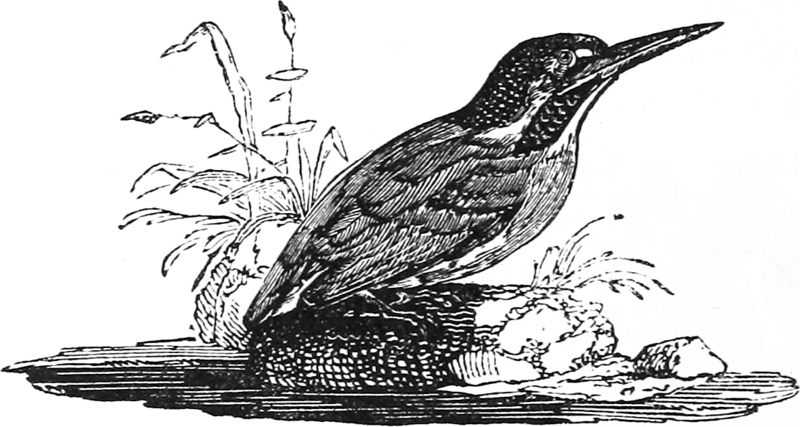
\includegraphics[scale=0.35]{images/Alycon.png}
        \end{figure}
        \vspace{0.5cm}
        \Huge
        \textbf{\textsc{Matematyka Dyskretna}}
        
        \vspace{0.5cm}
        \Large
        \textsc{Wybrane Dowody}
        
        \normalsize
        
        
        \line(1,0){330}
        
        \vspace{1cm}
        \textit{,,Myślę, że 7 punktów na 20 to nie jest zły wynik''}
        \vspace{1cm}

        \textit{\textsc{Popełnione przez}}\\
        \vspace{5mm}

        \textbf{\textsc{Dziurawy Ponton \\ Załatany Ponton \\ Puchaty Pompon \\ Zatopiony Ponton \\ Tonący Ponton \\ Notnop}}

        \vfill

        Kraków \\
        Anno Domini 2023
        
    \end{center}
    
\end{titlepage}


\tableofcontents
\section*{Licencja}
    \begin{figure}[h]
    	\begin{minipage}[c]{0.25\textwidth}
    		
\includegraphics[width=0.7\textwidth]{images/licencja.png}
    	\end{minipage}\hfill
    	\begin{minipage}[c]{0.75\textwidth}
    		\caption*{
    			Ten utwór jest dostępny na 
    			\href{https://creativecommons.org/licenses/by-sa/4.0/}{licencji Creative Commons Uznanie autorstwa
    			na tych samych warunkach 4.0 Międzynarodowe.}
    		}
    	\end{minipage}
    \end{figure}

% Actual content
\mainmatter

\chapter{Kombinatoryka}
 % Żeby nie było syfu to kolejne sekcje dodajemy do chapters/
% A potem includujemy za pomocą \input{chapters/...}

% Używamy \( \) i \[ \] zamiast dolarów -- tak jak się robi w LaTeXu


\documentclass[12pt, a4paper, polish, openany]{book}

% Please, let's familiarize ourselves with notatki.sty and tcs.sty so that we don't reinvent the wheel
\usepackage{notatki}

\fancyhead[L]{\textbf{\textit{MD}}}
\author{
}
\title{TCS and shitposting}


\begin{document}

% Front page and table of contents
\frontmatter

\begin{titlepage} 

    \begin{center}
         \begin{figure}[h]
            \centering
            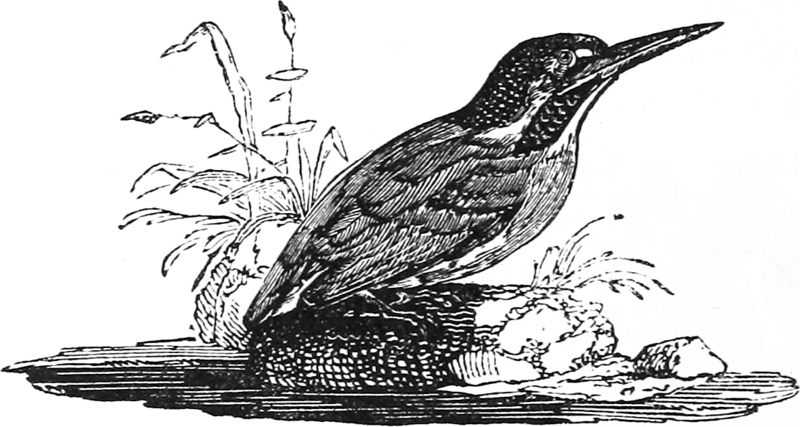
\includegraphics[scale=0.35]{images/Alycon.png}
        \end{figure}
        \vspace{0.5cm}
        \Huge
        \textbf{\textsc{Matematyka Dyskretna}}
        
        \vspace{0.5cm}
        \Large
        \textsc{Wybrane Dowody}
        
        \normalsize
        
        
        \line(1,0){330}
        
        \vspace{1cm}
        \textit{,,Myślę, że 7 punktów na 20 to nie jest zły wynik''}
        \vspace{1cm}

        \textit{\textsc{Popełnione przez}}\\
        \vspace{5mm}

        \textbf{\textsc{Dziurawy Ponton \\ Załatany Ponton \\ Puchaty Pompon \\ Zatopiony Ponton \\ Tonący Ponton \\ Notnop}}

        \vfill

        Kraków \\
        Anno Domini 2023
        
    \end{center}
    
\end{titlepage}


\tableofcontents
\section*{Licencja}
    \begin{figure}[h]
    	\begin{minipage}[c]{0.25\textwidth}
    		
\includegraphics[width=0.7\textwidth]{images/licencja.png}
    	\end{minipage}\hfill
    	\begin{minipage}[c]{0.75\textwidth}
    		\caption*{
    			Ten utwór jest dostępny na 
    			\href{https://creativecommons.org/licenses/by-sa/4.0/}{licencji Creative Commons Uznanie autorstwa
    			na tych samych warunkach 4.0 Międzynarodowe.}
    		}
    	\end{minipage}
    \end{figure}

% Actual content
\mainmatter

\chapter{Kombinatoryka}
 % Żeby nie było syfu to kolejne sekcje dodajemy do chapters/
% A potem includujemy za pomocą \input{chapters/...}

% Używamy \( \) i \[ \] zamiast dolarów -- tak jak się robi w LaTeXu


\documentclass[12pt, a4paper, polish, openany]{book}

% Please, let's familiarize ourselves with notatki.sty and tcs.sty so that we don't reinvent the wheel
\usepackage{notatki}

\fancyhead[L]{\textbf{\textit{MD}}}
\author{
}
\title{TCS and shitposting}


\begin{document}

% Front page and table of contents
\frontmatter

\input{titlepage}

\tableofcontents
\input{license}

% Actual content
\mainmatter

\chapter{Kombinatoryka}
\input{chapters/combinatorics/main}

\chapter{Zasada włączeń i wyłączeń}
\input{chapters/exclusion-inclusion/main}

\chapter{Posety}
\input{chapters/posets/main}

\chapter{Twierdzenie Ramseya}
\input{chapters/ramsey/main}

\chapter{Funkcje tworzące}
\input{chapters/generating_functions/main}

\chapter{Przepływy}
\input{chapters/flows/main}

\chapter{Skojarzenia}
\input{chapters/matchings/main}

\chapter{Kolorowanie grafów}
\input{chapters/graph-coloring/main}

\chapter{Grafy, ale nie kolorowanie}
\input{chapters/graph-misc/main}

\end{document}

\chapter{Zasada włączeń i wyłączeń}
 % Żeby nie było syfu to kolejne sekcje dodajemy do chapters/
% A potem includujemy za pomocą \input{chapters/...}

% Używamy \( \) i \[ \] zamiast dolarów -- tak jak się robi w LaTeXu


\documentclass[12pt, a4paper, polish, openany]{book}

% Please, let's familiarize ourselves with notatki.sty and tcs.sty so that we don't reinvent the wheel
\usepackage{notatki}

\fancyhead[L]{\textbf{\textit{MD}}}
\author{
}
\title{TCS and shitposting}


\begin{document}

% Front page and table of contents
\frontmatter

\input{titlepage}

\tableofcontents
\input{license}

% Actual content
\mainmatter

\chapter{Kombinatoryka}
\input{chapters/combinatorics/main}

\chapter{Zasada włączeń i wyłączeń}
\input{chapters/exclusion-inclusion/main}

\chapter{Posety}
\input{chapters/posets/main}

\chapter{Twierdzenie Ramseya}
\input{chapters/ramsey/main}

\chapter{Funkcje tworzące}
\input{chapters/generating_functions/main}

\chapter{Przepływy}
\input{chapters/flows/main}

\chapter{Skojarzenia}
\input{chapters/matchings/main}

\chapter{Kolorowanie grafów}
\input{chapters/graph-coloring/main}

\chapter{Grafy, ale nie kolorowanie}
\input{chapters/graph-misc/main}

\end{document}

\chapter{Posety}
 % Żeby nie było syfu to kolejne sekcje dodajemy do chapters/
% A potem includujemy za pomocą \input{chapters/...}

% Używamy \( \) i \[ \] zamiast dolarów -- tak jak się robi w LaTeXu


\documentclass[12pt, a4paper, polish, openany]{book}

% Please, let's familiarize ourselves with notatki.sty and tcs.sty so that we don't reinvent the wheel
\usepackage{notatki}

\fancyhead[L]{\textbf{\textit{MD}}}
\author{
}
\title{TCS and shitposting}


\begin{document}

% Front page and table of contents
\frontmatter

\input{titlepage}

\tableofcontents
\input{license}

% Actual content
\mainmatter

\chapter{Kombinatoryka}
\input{chapters/combinatorics/main}

\chapter{Zasada włączeń i wyłączeń}
\input{chapters/exclusion-inclusion/main}

\chapter{Posety}
\input{chapters/posets/main}

\chapter{Twierdzenie Ramseya}
\input{chapters/ramsey/main}

\chapter{Funkcje tworzące}
\input{chapters/generating_functions/main}

\chapter{Przepływy}
\input{chapters/flows/main}

\chapter{Skojarzenia}
\input{chapters/matchings/main}

\chapter{Kolorowanie grafów}
\input{chapters/graph-coloring/main}

\chapter{Grafy, ale nie kolorowanie}
\input{chapters/graph-misc/main}

\end{document}

\chapter{Twierdzenie Ramseya}
 % Żeby nie było syfu to kolejne sekcje dodajemy do chapters/
% A potem includujemy za pomocą \input{chapters/...}

% Używamy \( \) i \[ \] zamiast dolarów -- tak jak się robi w LaTeXu


\documentclass[12pt, a4paper, polish, openany]{book}

% Please, let's familiarize ourselves with notatki.sty and tcs.sty so that we don't reinvent the wheel
\usepackage{notatki}

\fancyhead[L]{\textbf{\textit{MD}}}
\author{
}
\title{TCS and shitposting}


\begin{document}

% Front page and table of contents
\frontmatter

\input{titlepage}

\tableofcontents
\input{license}

% Actual content
\mainmatter

\chapter{Kombinatoryka}
\input{chapters/combinatorics/main}

\chapter{Zasada włączeń i wyłączeń}
\input{chapters/exclusion-inclusion/main}

\chapter{Posety}
\input{chapters/posets/main}

\chapter{Twierdzenie Ramseya}
\input{chapters/ramsey/main}

\chapter{Funkcje tworzące}
\input{chapters/generating_functions/main}

\chapter{Przepływy}
\input{chapters/flows/main}

\chapter{Skojarzenia}
\input{chapters/matchings/main}

\chapter{Kolorowanie grafów}
\input{chapters/graph-coloring/main}

\chapter{Grafy, ale nie kolorowanie}
\input{chapters/graph-misc/main}

\end{document}

\chapter{Funkcje tworzące}
 % Żeby nie było syfu to kolejne sekcje dodajemy do chapters/
% A potem includujemy za pomocą \input{chapters/...}

% Używamy \( \) i \[ \] zamiast dolarów -- tak jak się robi w LaTeXu


\documentclass[12pt, a4paper, polish, openany]{book}

% Please, let's familiarize ourselves with notatki.sty and tcs.sty so that we don't reinvent the wheel
\usepackage{notatki}

\fancyhead[L]{\textbf{\textit{MD}}}
\author{
}
\title{TCS and shitposting}


\begin{document}

% Front page and table of contents
\frontmatter

\input{titlepage}

\tableofcontents
\input{license}

% Actual content
\mainmatter

\chapter{Kombinatoryka}
\input{chapters/combinatorics/main}

\chapter{Zasada włączeń i wyłączeń}
\input{chapters/exclusion-inclusion/main}

\chapter{Posety}
\input{chapters/posets/main}

\chapter{Twierdzenie Ramseya}
\input{chapters/ramsey/main}

\chapter{Funkcje tworzące}
\input{chapters/generating_functions/main}

\chapter{Przepływy}
\input{chapters/flows/main}

\chapter{Skojarzenia}
\input{chapters/matchings/main}

\chapter{Kolorowanie grafów}
\input{chapters/graph-coloring/main}

\chapter{Grafy, ale nie kolorowanie}
\input{chapters/graph-misc/main}

\end{document}

\chapter{Przepływy}
 % Żeby nie było syfu to kolejne sekcje dodajemy do chapters/
% A potem includujemy za pomocą \input{chapters/...}

% Używamy \( \) i \[ \] zamiast dolarów -- tak jak się robi w LaTeXu


\documentclass[12pt, a4paper, polish, openany]{book}

% Please, let's familiarize ourselves with notatki.sty and tcs.sty so that we don't reinvent the wheel
\usepackage{notatki}

\fancyhead[L]{\textbf{\textit{MD}}}
\author{
}
\title{TCS and shitposting}


\begin{document}

% Front page and table of contents
\frontmatter

\input{titlepage}

\tableofcontents
\input{license}

% Actual content
\mainmatter

\chapter{Kombinatoryka}
\input{chapters/combinatorics/main}

\chapter{Zasada włączeń i wyłączeń}
\input{chapters/exclusion-inclusion/main}

\chapter{Posety}
\input{chapters/posets/main}

\chapter{Twierdzenie Ramseya}
\input{chapters/ramsey/main}

\chapter{Funkcje tworzące}
\input{chapters/generating_functions/main}

\chapter{Przepływy}
\input{chapters/flows/main}

\chapter{Skojarzenia}
\input{chapters/matchings/main}

\chapter{Kolorowanie grafów}
\input{chapters/graph-coloring/main}

\chapter{Grafy, ale nie kolorowanie}
\input{chapters/graph-misc/main}

\end{document}

\chapter{Skojarzenia}
 % Żeby nie było syfu to kolejne sekcje dodajemy do chapters/
% A potem includujemy za pomocą \input{chapters/...}

% Używamy \( \) i \[ \] zamiast dolarów -- tak jak się robi w LaTeXu


\documentclass[12pt, a4paper, polish, openany]{book}

% Please, let's familiarize ourselves with notatki.sty and tcs.sty so that we don't reinvent the wheel
\usepackage{notatki}

\fancyhead[L]{\textbf{\textit{MD}}}
\author{
}
\title{TCS and shitposting}


\begin{document}

% Front page and table of contents
\frontmatter

\input{titlepage}

\tableofcontents
\input{license}

% Actual content
\mainmatter

\chapter{Kombinatoryka}
\input{chapters/combinatorics/main}

\chapter{Zasada włączeń i wyłączeń}
\input{chapters/exclusion-inclusion/main}

\chapter{Posety}
\input{chapters/posets/main}

\chapter{Twierdzenie Ramseya}
\input{chapters/ramsey/main}

\chapter{Funkcje tworzące}
\input{chapters/generating_functions/main}

\chapter{Przepływy}
\input{chapters/flows/main}

\chapter{Skojarzenia}
\input{chapters/matchings/main}

\chapter{Kolorowanie grafów}
\input{chapters/graph-coloring/main}

\chapter{Grafy, ale nie kolorowanie}
\input{chapters/graph-misc/main}

\end{document}

\chapter{Kolorowanie grafów}
 % Żeby nie było syfu to kolejne sekcje dodajemy do chapters/
% A potem includujemy za pomocą \input{chapters/...}

% Używamy \( \) i \[ \] zamiast dolarów -- tak jak się robi w LaTeXu


\documentclass[12pt, a4paper, polish, openany]{book}

% Please, let's familiarize ourselves with notatki.sty and tcs.sty so that we don't reinvent the wheel
\usepackage{notatki}

\fancyhead[L]{\textbf{\textit{MD}}}
\author{
}
\title{TCS and shitposting}


\begin{document}

% Front page and table of contents
\frontmatter

\input{titlepage}

\tableofcontents
\input{license}

% Actual content
\mainmatter

\chapter{Kombinatoryka}
\input{chapters/combinatorics/main}

\chapter{Zasada włączeń i wyłączeń}
\input{chapters/exclusion-inclusion/main}

\chapter{Posety}
\input{chapters/posets/main}

\chapter{Twierdzenie Ramseya}
\input{chapters/ramsey/main}

\chapter{Funkcje tworzące}
\input{chapters/generating_functions/main}

\chapter{Przepływy}
\input{chapters/flows/main}

\chapter{Skojarzenia}
\input{chapters/matchings/main}

\chapter{Kolorowanie grafów}
\input{chapters/graph-coloring/main}

\chapter{Grafy, ale nie kolorowanie}
\input{chapters/graph-misc/main}

\end{document}

\chapter{Grafy, ale nie kolorowanie}
 % Żeby nie było syfu to kolejne sekcje dodajemy do chapters/
% A potem includujemy za pomocą \input{chapters/...}

% Używamy \( \) i \[ \] zamiast dolarów -- tak jak się robi w LaTeXu


\documentclass[12pt, a4paper, polish, openany]{book}

% Please, let's familiarize ourselves with notatki.sty and tcs.sty so that we don't reinvent the wheel
\usepackage{notatki}

\fancyhead[L]{\textbf{\textit{MD}}}
\author{
}
\title{TCS and shitposting}


\begin{document}

% Front page and table of contents
\frontmatter

\input{titlepage}

\tableofcontents
\input{license}

% Actual content
\mainmatter

\chapter{Kombinatoryka}
\input{chapters/combinatorics/main}

\chapter{Zasada włączeń i wyłączeń}
\input{chapters/exclusion-inclusion/main}

\chapter{Posety}
\input{chapters/posets/main}

\chapter{Twierdzenie Ramseya}
\input{chapters/ramsey/main}

\chapter{Funkcje tworzące}
\input{chapters/generating_functions/main}

\chapter{Przepływy}
\input{chapters/flows/main}

\chapter{Skojarzenia}
\input{chapters/matchings/main}

\chapter{Kolorowanie grafów}
\input{chapters/graph-coloring/main}

\chapter{Grafy, ale nie kolorowanie}
\input{chapters/graph-misc/main}

\end{document}

\end{document}

\chapter{Zasada włączeń i wyłączeń}
 % Żeby nie było syfu to kolejne sekcje dodajemy do chapters/
% A potem includujemy za pomocą \input{chapters/...}

% Używamy \( \) i \[ \] zamiast dolarów -- tak jak się robi w LaTeXu


\documentclass[12pt, a4paper, polish, openany]{book}

% Please, let's familiarize ourselves with notatki.sty and tcs.sty so that we don't reinvent the wheel
\usepackage{notatki}

\fancyhead[L]{\textbf{\textit{MD}}}
\author{
}
\title{TCS and shitposting}


\begin{document}

% Front page and table of contents
\frontmatter

\begin{titlepage} 

    \begin{center}
         \begin{figure}[h]
            \centering
            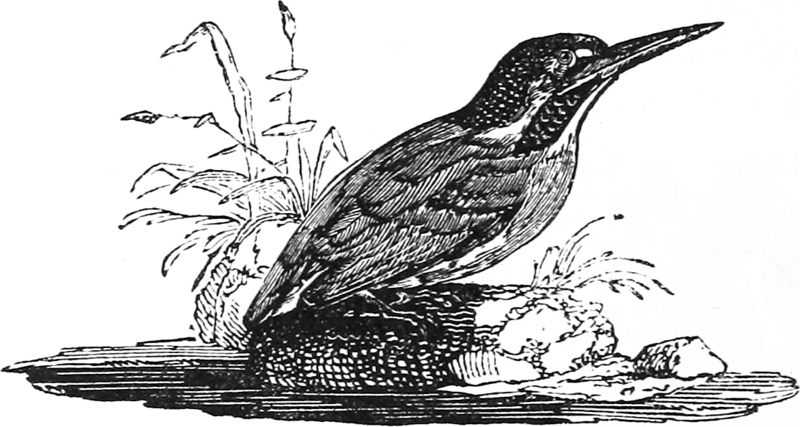
\includegraphics[scale=0.35]{images/Alycon.png}
        \end{figure}
        \vspace{0.5cm}
        \Huge
        \textbf{\textsc{Matematyka Dyskretna}}
        
        \vspace{0.5cm}
        \Large
        \textsc{Wybrane Dowody}
        
        \normalsize
        
        
        \line(1,0){330}
        
        \vspace{1cm}
        \textit{,,Myślę, że 7 punktów na 20 to nie jest zły wynik''}
        \vspace{1cm}

        \textit{\textsc{Popełnione przez}}\\
        \vspace{5mm}

        \textbf{\textsc{Dziurawy Ponton \\ Załatany Ponton \\ Puchaty Pompon \\ Zatopiony Ponton \\ Tonący Ponton \\ Notnop}}

        \vfill

        Kraków \\
        Anno Domini 2023
        
    \end{center}
    
\end{titlepage}


\tableofcontents
\section*{Licencja}
    \begin{figure}[h]
    	\begin{minipage}[c]{0.25\textwidth}
    		
\includegraphics[width=0.7\textwidth]{images/licencja.png}
    	\end{minipage}\hfill
    	\begin{minipage}[c]{0.75\textwidth}
    		\caption*{
    			Ten utwór jest dostępny na 
    			\href{https://creativecommons.org/licenses/by-sa/4.0/}{licencji Creative Commons Uznanie autorstwa
    			na tych samych warunkach 4.0 Międzynarodowe.}
    		}
    	\end{minipage}
    \end{figure}

% Actual content
\mainmatter

\chapter{Kombinatoryka}
 % Żeby nie było syfu to kolejne sekcje dodajemy do chapters/
% A potem includujemy za pomocą \input{chapters/...}

% Używamy \( \) i \[ \] zamiast dolarów -- tak jak się robi w LaTeXu


\documentclass[12pt, a4paper, polish, openany]{book}

% Please, let's familiarize ourselves with notatki.sty and tcs.sty so that we don't reinvent the wheel
\usepackage{notatki}

\fancyhead[L]{\textbf{\textit{MD}}}
\author{
}
\title{TCS and shitposting}


\begin{document}

% Front page and table of contents
\frontmatter

\input{titlepage}

\tableofcontents
\input{license}

% Actual content
\mainmatter

\chapter{Kombinatoryka}
\input{chapters/combinatorics/main}

\chapter{Zasada włączeń i wyłączeń}
\input{chapters/exclusion-inclusion/main}

\chapter{Posety}
\input{chapters/posets/main}

\chapter{Twierdzenie Ramseya}
\input{chapters/ramsey/main}

\chapter{Funkcje tworzące}
\input{chapters/generating_functions/main}

\chapter{Przepływy}
\input{chapters/flows/main}

\chapter{Skojarzenia}
\input{chapters/matchings/main}

\chapter{Kolorowanie grafów}
\input{chapters/graph-coloring/main}

\chapter{Grafy, ale nie kolorowanie}
\input{chapters/graph-misc/main}

\end{document}

\chapter{Zasada włączeń i wyłączeń}
 % Żeby nie było syfu to kolejne sekcje dodajemy do chapters/
% A potem includujemy za pomocą \input{chapters/...}

% Używamy \( \) i \[ \] zamiast dolarów -- tak jak się robi w LaTeXu


\documentclass[12pt, a4paper, polish, openany]{book}

% Please, let's familiarize ourselves with notatki.sty and tcs.sty so that we don't reinvent the wheel
\usepackage{notatki}

\fancyhead[L]{\textbf{\textit{MD}}}
\author{
}
\title{TCS and shitposting}


\begin{document}

% Front page and table of contents
\frontmatter

\input{titlepage}

\tableofcontents
\input{license}

% Actual content
\mainmatter

\chapter{Kombinatoryka}
\input{chapters/combinatorics/main}

\chapter{Zasada włączeń i wyłączeń}
\input{chapters/exclusion-inclusion/main}

\chapter{Posety}
\input{chapters/posets/main}

\chapter{Twierdzenie Ramseya}
\input{chapters/ramsey/main}

\chapter{Funkcje tworzące}
\input{chapters/generating_functions/main}

\chapter{Przepływy}
\input{chapters/flows/main}

\chapter{Skojarzenia}
\input{chapters/matchings/main}

\chapter{Kolorowanie grafów}
\input{chapters/graph-coloring/main}

\chapter{Grafy, ale nie kolorowanie}
\input{chapters/graph-misc/main}

\end{document}

\chapter{Posety}
 % Żeby nie było syfu to kolejne sekcje dodajemy do chapters/
% A potem includujemy za pomocą \input{chapters/...}

% Używamy \( \) i \[ \] zamiast dolarów -- tak jak się robi w LaTeXu


\documentclass[12pt, a4paper, polish, openany]{book}

% Please, let's familiarize ourselves with notatki.sty and tcs.sty so that we don't reinvent the wheel
\usepackage{notatki}

\fancyhead[L]{\textbf{\textit{MD}}}
\author{
}
\title{TCS and shitposting}


\begin{document}

% Front page and table of contents
\frontmatter

\input{titlepage}

\tableofcontents
\input{license}

% Actual content
\mainmatter

\chapter{Kombinatoryka}
\input{chapters/combinatorics/main}

\chapter{Zasada włączeń i wyłączeń}
\input{chapters/exclusion-inclusion/main}

\chapter{Posety}
\input{chapters/posets/main}

\chapter{Twierdzenie Ramseya}
\input{chapters/ramsey/main}

\chapter{Funkcje tworzące}
\input{chapters/generating_functions/main}

\chapter{Przepływy}
\input{chapters/flows/main}

\chapter{Skojarzenia}
\input{chapters/matchings/main}

\chapter{Kolorowanie grafów}
\input{chapters/graph-coloring/main}

\chapter{Grafy, ale nie kolorowanie}
\input{chapters/graph-misc/main}

\end{document}

\chapter{Twierdzenie Ramseya}
 % Żeby nie było syfu to kolejne sekcje dodajemy do chapters/
% A potem includujemy za pomocą \input{chapters/...}

% Używamy \( \) i \[ \] zamiast dolarów -- tak jak się robi w LaTeXu


\documentclass[12pt, a4paper, polish, openany]{book}

% Please, let's familiarize ourselves with notatki.sty and tcs.sty so that we don't reinvent the wheel
\usepackage{notatki}

\fancyhead[L]{\textbf{\textit{MD}}}
\author{
}
\title{TCS and shitposting}


\begin{document}

% Front page and table of contents
\frontmatter

\input{titlepage}

\tableofcontents
\input{license}

% Actual content
\mainmatter

\chapter{Kombinatoryka}
\input{chapters/combinatorics/main}

\chapter{Zasada włączeń i wyłączeń}
\input{chapters/exclusion-inclusion/main}

\chapter{Posety}
\input{chapters/posets/main}

\chapter{Twierdzenie Ramseya}
\input{chapters/ramsey/main}

\chapter{Funkcje tworzące}
\input{chapters/generating_functions/main}

\chapter{Przepływy}
\input{chapters/flows/main}

\chapter{Skojarzenia}
\input{chapters/matchings/main}

\chapter{Kolorowanie grafów}
\input{chapters/graph-coloring/main}

\chapter{Grafy, ale nie kolorowanie}
\input{chapters/graph-misc/main}

\end{document}

\chapter{Funkcje tworzące}
 % Żeby nie było syfu to kolejne sekcje dodajemy do chapters/
% A potem includujemy za pomocą \input{chapters/...}

% Używamy \( \) i \[ \] zamiast dolarów -- tak jak się robi w LaTeXu


\documentclass[12pt, a4paper, polish, openany]{book}

% Please, let's familiarize ourselves with notatki.sty and tcs.sty so that we don't reinvent the wheel
\usepackage{notatki}

\fancyhead[L]{\textbf{\textit{MD}}}
\author{
}
\title{TCS and shitposting}


\begin{document}

% Front page and table of contents
\frontmatter

\input{titlepage}

\tableofcontents
\input{license}

% Actual content
\mainmatter

\chapter{Kombinatoryka}
\input{chapters/combinatorics/main}

\chapter{Zasada włączeń i wyłączeń}
\input{chapters/exclusion-inclusion/main}

\chapter{Posety}
\input{chapters/posets/main}

\chapter{Twierdzenie Ramseya}
\input{chapters/ramsey/main}

\chapter{Funkcje tworzące}
\input{chapters/generating_functions/main}

\chapter{Przepływy}
\input{chapters/flows/main}

\chapter{Skojarzenia}
\input{chapters/matchings/main}

\chapter{Kolorowanie grafów}
\input{chapters/graph-coloring/main}

\chapter{Grafy, ale nie kolorowanie}
\input{chapters/graph-misc/main}

\end{document}

\chapter{Przepływy}
 % Żeby nie było syfu to kolejne sekcje dodajemy do chapters/
% A potem includujemy za pomocą \input{chapters/...}

% Używamy \( \) i \[ \] zamiast dolarów -- tak jak się robi w LaTeXu


\documentclass[12pt, a4paper, polish, openany]{book}

% Please, let's familiarize ourselves with notatki.sty and tcs.sty so that we don't reinvent the wheel
\usepackage{notatki}

\fancyhead[L]{\textbf{\textit{MD}}}
\author{
}
\title{TCS and shitposting}


\begin{document}

% Front page and table of contents
\frontmatter

\input{titlepage}

\tableofcontents
\input{license}

% Actual content
\mainmatter

\chapter{Kombinatoryka}
\input{chapters/combinatorics/main}

\chapter{Zasada włączeń i wyłączeń}
\input{chapters/exclusion-inclusion/main}

\chapter{Posety}
\input{chapters/posets/main}

\chapter{Twierdzenie Ramseya}
\input{chapters/ramsey/main}

\chapter{Funkcje tworzące}
\input{chapters/generating_functions/main}

\chapter{Przepływy}
\input{chapters/flows/main}

\chapter{Skojarzenia}
\input{chapters/matchings/main}

\chapter{Kolorowanie grafów}
\input{chapters/graph-coloring/main}

\chapter{Grafy, ale nie kolorowanie}
\input{chapters/graph-misc/main}

\end{document}

\chapter{Skojarzenia}
 % Żeby nie było syfu to kolejne sekcje dodajemy do chapters/
% A potem includujemy za pomocą \input{chapters/...}

% Używamy \( \) i \[ \] zamiast dolarów -- tak jak się robi w LaTeXu


\documentclass[12pt, a4paper, polish, openany]{book}

% Please, let's familiarize ourselves with notatki.sty and tcs.sty so that we don't reinvent the wheel
\usepackage{notatki}

\fancyhead[L]{\textbf{\textit{MD}}}
\author{
}
\title{TCS and shitposting}


\begin{document}

% Front page and table of contents
\frontmatter

\input{titlepage}

\tableofcontents
\input{license}

% Actual content
\mainmatter

\chapter{Kombinatoryka}
\input{chapters/combinatorics/main}

\chapter{Zasada włączeń i wyłączeń}
\input{chapters/exclusion-inclusion/main}

\chapter{Posety}
\input{chapters/posets/main}

\chapter{Twierdzenie Ramseya}
\input{chapters/ramsey/main}

\chapter{Funkcje tworzące}
\input{chapters/generating_functions/main}

\chapter{Przepływy}
\input{chapters/flows/main}

\chapter{Skojarzenia}
\input{chapters/matchings/main}

\chapter{Kolorowanie grafów}
\input{chapters/graph-coloring/main}

\chapter{Grafy, ale nie kolorowanie}
\input{chapters/graph-misc/main}

\end{document}

\chapter{Kolorowanie grafów}
 % Żeby nie było syfu to kolejne sekcje dodajemy do chapters/
% A potem includujemy za pomocą \input{chapters/...}

% Używamy \( \) i \[ \] zamiast dolarów -- tak jak się robi w LaTeXu


\documentclass[12pt, a4paper, polish, openany]{book}

% Please, let's familiarize ourselves with notatki.sty and tcs.sty so that we don't reinvent the wheel
\usepackage{notatki}

\fancyhead[L]{\textbf{\textit{MD}}}
\author{
}
\title{TCS and shitposting}


\begin{document}

% Front page and table of contents
\frontmatter

\input{titlepage}

\tableofcontents
\input{license}

% Actual content
\mainmatter

\chapter{Kombinatoryka}
\input{chapters/combinatorics/main}

\chapter{Zasada włączeń i wyłączeń}
\input{chapters/exclusion-inclusion/main}

\chapter{Posety}
\input{chapters/posets/main}

\chapter{Twierdzenie Ramseya}
\input{chapters/ramsey/main}

\chapter{Funkcje tworzące}
\input{chapters/generating_functions/main}

\chapter{Przepływy}
\input{chapters/flows/main}

\chapter{Skojarzenia}
\input{chapters/matchings/main}

\chapter{Kolorowanie grafów}
\input{chapters/graph-coloring/main}

\chapter{Grafy, ale nie kolorowanie}
\input{chapters/graph-misc/main}

\end{document}

\chapter{Grafy, ale nie kolorowanie}
 % Żeby nie było syfu to kolejne sekcje dodajemy do chapters/
% A potem includujemy za pomocą \input{chapters/...}

% Używamy \( \) i \[ \] zamiast dolarów -- tak jak się robi w LaTeXu


\documentclass[12pt, a4paper, polish, openany]{book}

% Please, let's familiarize ourselves with notatki.sty and tcs.sty so that we don't reinvent the wheel
\usepackage{notatki}

\fancyhead[L]{\textbf{\textit{MD}}}
\author{
}
\title{TCS and shitposting}


\begin{document}

% Front page and table of contents
\frontmatter

\input{titlepage}

\tableofcontents
\input{license}

% Actual content
\mainmatter

\chapter{Kombinatoryka}
\input{chapters/combinatorics/main}

\chapter{Zasada włączeń i wyłączeń}
\input{chapters/exclusion-inclusion/main}

\chapter{Posety}
\input{chapters/posets/main}

\chapter{Twierdzenie Ramseya}
\input{chapters/ramsey/main}

\chapter{Funkcje tworzące}
\input{chapters/generating_functions/main}

\chapter{Przepływy}
\input{chapters/flows/main}

\chapter{Skojarzenia}
\input{chapters/matchings/main}

\chapter{Kolorowanie grafów}
\input{chapters/graph-coloring/main}

\chapter{Grafy, ale nie kolorowanie}
\input{chapters/graph-misc/main}

\end{document}

\end{document}

\chapter{Posety}
 % Żeby nie było syfu to kolejne sekcje dodajemy do chapters/
% A potem includujemy za pomocą \input{chapters/...}

% Używamy \( \) i \[ \] zamiast dolarów -- tak jak się robi w LaTeXu


\documentclass[12pt, a4paper, polish, openany]{book}

% Please, let's familiarize ourselves with notatki.sty and tcs.sty so that we don't reinvent the wheel
\usepackage{notatki}

\fancyhead[L]{\textbf{\textit{MD}}}
\author{
}
\title{TCS and shitposting}


\begin{document}

% Front page and table of contents
\frontmatter

\begin{titlepage} 

    \begin{center}
         \begin{figure}[h]
            \centering
            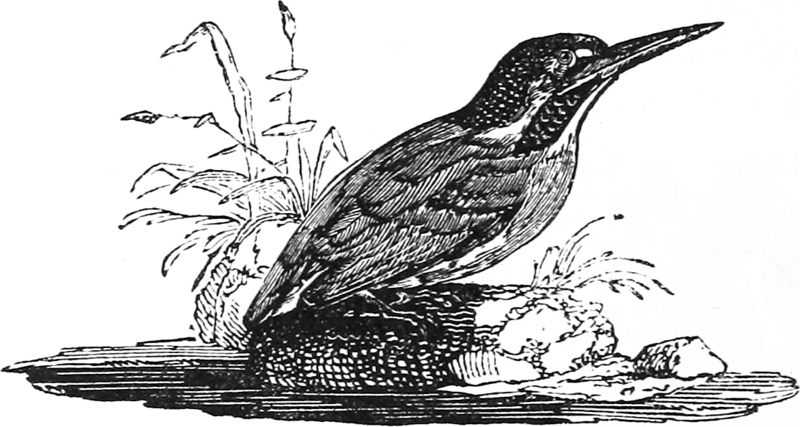
\includegraphics[scale=0.35]{images/Alycon.png}
        \end{figure}
        \vspace{0.5cm}
        \Huge
        \textbf{\textsc{Matematyka Dyskretna}}
        
        \vspace{0.5cm}
        \Large
        \textsc{Wybrane Dowody}
        
        \normalsize
        
        
        \line(1,0){330}
        
        \vspace{1cm}
        \textit{,,Myślę, że 7 punktów na 20 to nie jest zły wynik''}
        \vspace{1cm}

        \textit{\textsc{Popełnione przez}}\\
        \vspace{5mm}

        \textbf{\textsc{Dziurawy Ponton \\ Załatany Ponton \\ Puchaty Pompon \\ Zatopiony Ponton \\ Tonący Ponton \\ Notnop}}

        \vfill

        Kraków \\
        Anno Domini 2023
        
    \end{center}
    
\end{titlepage}


\tableofcontents
\section*{Licencja}
    \begin{figure}[h]
    	\begin{minipage}[c]{0.25\textwidth}
    		
\includegraphics[width=0.7\textwidth]{images/licencja.png}
    	\end{minipage}\hfill
    	\begin{minipage}[c]{0.75\textwidth}
    		\caption*{
    			Ten utwór jest dostępny na 
    			\href{https://creativecommons.org/licenses/by-sa/4.0/}{licencji Creative Commons Uznanie autorstwa
    			na tych samych warunkach 4.0 Międzynarodowe.}
    		}
    	\end{minipage}
    \end{figure}

% Actual content
\mainmatter

\chapter{Kombinatoryka}
 % Żeby nie było syfu to kolejne sekcje dodajemy do chapters/
% A potem includujemy za pomocą \input{chapters/...}

% Używamy \( \) i \[ \] zamiast dolarów -- tak jak się robi w LaTeXu


\documentclass[12pt, a4paper, polish, openany]{book}

% Please, let's familiarize ourselves with notatki.sty and tcs.sty so that we don't reinvent the wheel
\usepackage{notatki}

\fancyhead[L]{\textbf{\textit{MD}}}
\author{
}
\title{TCS and shitposting}


\begin{document}

% Front page and table of contents
\frontmatter

\input{titlepage}

\tableofcontents
\input{license}

% Actual content
\mainmatter

\chapter{Kombinatoryka}
\input{chapters/combinatorics/main}

\chapter{Zasada włączeń i wyłączeń}
\input{chapters/exclusion-inclusion/main}

\chapter{Posety}
\input{chapters/posets/main}

\chapter{Twierdzenie Ramseya}
\input{chapters/ramsey/main}

\chapter{Funkcje tworzące}
\input{chapters/generating_functions/main}

\chapter{Przepływy}
\input{chapters/flows/main}

\chapter{Skojarzenia}
\input{chapters/matchings/main}

\chapter{Kolorowanie grafów}
\input{chapters/graph-coloring/main}

\chapter{Grafy, ale nie kolorowanie}
\input{chapters/graph-misc/main}

\end{document}

\chapter{Zasada włączeń i wyłączeń}
 % Żeby nie było syfu to kolejne sekcje dodajemy do chapters/
% A potem includujemy za pomocą \input{chapters/...}

% Używamy \( \) i \[ \] zamiast dolarów -- tak jak się robi w LaTeXu


\documentclass[12pt, a4paper, polish, openany]{book}

% Please, let's familiarize ourselves with notatki.sty and tcs.sty so that we don't reinvent the wheel
\usepackage{notatki}

\fancyhead[L]{\textbf{\textit{MD}}}
\author{
}
\title{TCS and shitposting}


\begin{document}

% Front page and table of contents
\frontmatter

\input{titlepage}

\tableofcontents
\input{license}

% Actual content
\mainmatter

\chapter{Kombinatoryka}
\input{chapters/combinatorics/main}

\chapter{Zasada włączeń i wyłączeń}
\input{chapters/exclusion-inclusion/main}

\chapter{Posety}
\input{chapters/posets/main}

\chapter{Twierdzenie Ramseya}
\input{chapters/ramsey/main}

\chapter{Funkcje tworzące}
\input{chapters/generating_functions/main}

\chapter{Przepływy}
\input{chapters/flows/main}

\chapter{Skojarzenia}
\input{chapters/matchings/main}

\chapter{Kolorowanie grafów}
\input{chapters/graph-coloring/main}

\chapter{Grafy, ale nie kolorowanie}
\input{chapters/graph-misc/main}

\end{document}

\chapter{Posety}
 % Żeby nie było syfu to kolejne sekcje dodajemy do chapters/
% A potem includujemy za pomocą \input{chapters/...}

% Używamy \( \) i \[ \] zamiast dolarów -- tak jak się robi w LaTeXu


\documentclass[12pt, a4paper, polish, openany]{book}

% Please, let's familiarize ourselves with notatki.sty and tcs.sty so that we don't reinvent the wheel
\usepackage{notatki}

\fancyhead[L]{\textbf{\textit{MD}}}
\author{
}
\title{TCS and shitposting}


\begin{document}

% Front page and table of contents
\frontmatter

\input{titlepage}

\tableofcontents
\input{license}

% Actual content
\mainmatter

\chapter{Kombinatoryka}
\input{chapters/combinatorics/main}

\chapter{Zasada włączeń i wyłączeń}
\input{chapters/exclusion-inclusion/main}

\chapter{Posety}
\input{chapters/posets/main}

\chapter{Twierdzenie Ramseya}
\input{chapters/ramsey/main}

\chapter{Funkcje tworzące}
\input{chapters/generating_functions/main}

\chapter{Przepływy}
\input{chapters/flows/main}

\chapter{Skojarzenia}
\input{chapters/matchings/main}

\chapter{Kolorowanie grafów}
\input{chapters/graph-coloring/main}

\chapter{Grafy, ale nie kolorowanie}
\input{chapters/graph-misc/main}

\end{document}

\chapter{Twierdzenie Ramseya}
 % Żeby nie było syfu to kolejne sekcje dodajemy do chapters/
% A potem includujemy za pomocą \input{chapters/...}

% Używamy \( \) i \[ \] zamiast dolarów -- tak jak się robi w LaTeXu


\documentclass[12pt, a4paper, polish, openany]{book}

% Please, let's familiarize ourselves with notatki.sty and tcs.sty so that we don't reinvent the wheel
\usepackage{notatki}

\fancyhead[L]{\textbf{\textit{MD}}}
\author{
}
\title{TCS and shitposting}


\begin{document}

% Front page and table of contents
\frontmatter

\input{titlepage}

\tableofcontents
\input{license}

% Actual content
\mainmatter

\chapter{Kombinatoryka}
\input{chapters/combinatorics/main}

\chapter{Zasada włączeń i wyłączeń}
\input{chapters/exclusion-inclusion/main}

\chapter{Posety}
\input{chapters/posets/main}

\chapter{Twierdzenie Ramseya}
\input{chapters/ramsey/main}

\chapter{Funkcje tworzące}
\input{chapters/generating_functions/main}

\chapter{Przepływy}
\input{chapters/flows/main}

\chapter{Skojarzenia}
\input{chapters/matchings/main}

\chapter{Kolorowanie grafów}
\input{chapters/graph-coloring/main}

\chapter{Grafy, ale nie kolorowanie}
\input{chapters/graph-misc/main}

\end{document}

\chapter{Funkcje tworzące}
 % Żeby nie było syfu to kolejne sekcje dodajemy do chapters/
% A potem includujemy za pomocą \input{chapters/...}

% Używamy \( \) i \[ \] zamiast dolarów -- tak jak się robi w LaTeXu


\documentclass[12pt, a4paper, polish, openany]{book}

% Please, let's familiarize ourselves with notatki.sty and tcs.sty so that we don't reinvent the wheel
\usepackage{notatki}

\fancyhead[L]{\textbf{\textit{MD}}}
\author{
}
\title{TCS and shitposting}


\begin{document}

% Front page and table of contents
\frontmatter

\input{titlepage}

\tableofcontents
\input{license}

% Actual content
\mainmatter

\chapter{Kombinatoryka}
\input{chapters/combinatorics/main}

\chapter{Zasada włączeń i wyłączeń}
\input{chapters/exclusion-inclusion/main}

\chapter{Posety}
\input{chapters/posets/main}

\chapter{Twierdzenie Ramseya}
\input{chapters/ramsey/main}

\chapter{Funkcje tworzące}
\input{chapters/generating_functions/main}

\chapter{Przepływy}
\input{chapters/flows/main}

\chapter{Skojarzenia}
\input{chapters/matchings/main}

\chapter{Kolorowanie grafów}
\input{chapters/graph-coloring/main}

\chapter{Grafy, ale nie kolorowanie}
\input{chapters/graph-misc/main}

\end{document}

\chapter{Przepływy}
 % Żeby nie było syfu to kolejne sekcje dodajemy do chapters/
% A potem includujemy za pomocą \input{chapters/...}

% Używamy \( \) i \[ \] zamiast dolarów -- tak jak się robi w LaTeXu


\documentclass[12pt, a4paper, polish, openany]{book}

% Please, let's familiarize ourselves with notatki.sty and tcs.sty so that we don't reinvent the wheel
\usepackage{notatki}

\fancyhead[L]{\textbf{\textit{MD}}}
\author{
}
\title{TCS and shitposting}


\begin{document}

% Front page and table of contents
\frontmatter

\input{titlepage}

\tableofcontents
\input{license}

% Actual content
\mainmatter

\chapter{Kombinatoryka}
\input{chapters/combinatorics/main}

\chapter{Zasada włączeń i wyłączeń}
\input{chapters/exclusion-inclusion/main}

\chapter{Posety}
\input{chapters/posets/main}

\chapter{Twierdzenie Ramseya}
\input{chapters/ramsey/main}

\chapter{Funkcje tworzące}
\input{chapters/generating_functions/main}

\chapter{Przepływy}
\input{chapters/flows/main}

\chapter{Skojarzenia}
\input{chapters/matchings/main}

\chapter{Kolorowanie grafów}
\input{chapters/graph-coloring/main}

\chapter{Grafy, ale nie kolorowanie}
\input{chapters/graph-misc/main}

\end{document}

\chapter{Skojarzenia}
 % Żeby nie było syfu to kolejne sekcje dodajemy do chapters/
% A potem includujemy za pomocą \input{chapters/...}

% Używamy \( \) i \[ \] zamiast dolarów -- tak jak się robi w LaTeXu


\documentclass[12pt, a4paper, polish, openany]{book}

% Please, let's familiarize ourselves with notatki.sty and tcs.sty so that we don't reinvent the wheel
\usepackage{notatki}

\fancyhead[L]{\textbf{\textit{MD}}}
\author{
}
\title{TCS and shitposting}


\begin{document}

% Front page and table of contents
\frontmatter

\input{titlepage}

\tableofcontents
\input{license}

% Actual content
\mainmatter

\chapter{Kombinatoryka}
\input{chapters/combinatorics/main}

\chapter{Zasada włączeń i wyłączeń}
\input{chapters/exclusion-inclusion/main}

\chapter{Posety}
\input{chapters/posets/main}

\chapter{Twierdzenie Ramseya}
\input{chapters/ramsey/main}

\chapter{Funkcje tworzące}
\input{chapters/generating_functions/main}

\chapter{Przepływy}
\input{chapters/flows/main}

\chapter{Skojarzenia}
\input{chapters/matchings/main}

\chapter{Kolorowanie grafów}
\input{chapters/graph-coloring/main}

\chapter{Grafy, ale nie kolorowanie}
\input{chapters/graph-misc/main}

\end{document}

\chapter{Kolorowanie grafów}
 % Żeby nie było syfu to kolejne sekcje dodajemy do chapters/
% A potem includujemy za pomocą \input{chapters/...}

% Używamy \( \) i \[ \] zamiast dolarów -- tak jak się robi w LaTeXu


\documentclass[12pt, a4paper, polish, openany]{book}

% Please, let's familiarize ourselves with notatki.sty and tcs.sty so that we don't reinvent the wheel
\usepackage{notatki}

\fancyhead[L]{\textbf{\textit{MD}}}
\author{
}
\title{TCS and shitposting}


\begin{document}

% Front page and table of contents
\frontmatter

\input{titlepage}

\tableofcontents
\input{license}

% Actual content
\mainmatter

\chapter{Kombinatoryka}
\input{chapters/combinatorics/main}

\chapter{Zasada włączeń i wyłączeń}
\input{chapters/exclusion-inclusion/main}

\chapter{Posety}
\input{chapters/posets/main}

\chapter{Twierdzenie Ramseya}
\input{chapters/ramsey/main}

\chapter{Funkcje tworzące}
\input{chapters/generating_functions/main}

\chapter{Przepływy}
\input{chapters/flows/main}

\chapter{Skojarzenia}
\input{chapters/matchings/main}

\chapter{Kolorowanie grafów}
\input{chapters/graph-coloring/main}

\chapter{Grafy, ale nie kolorowanie}
\input{chapters/graph-misc/main}

\end{document}

\chapter{Grafy, ale nie kolorowanie}
 % Żeby nie było syfu to kolejne sekcje dodajemy do chapters/
% A potem includujemy za pomocą \input{chapters/...}

% Używamy \( \) i \[ \] zamiast dolarów -- tak jak się robi w LaTeXu


\documentclass[12pt, a4paper, polish, openany]{book}

% Please, let's familiarize ourselves with notatki.sty and tcs.sty so that we don't reinvent the wheel
\usepackage{notatki}

\fancyhead[L]{\textbf{\textit{MD}}}
\author{
}
\title{TCS and shitposting}


\begin{document}

% Front page and table of contents
\frontmatter

\input{titlepage}

\tableofcontents
\input{license}

% Actual content
\mainmatter

\chapter{Kombinatoryka}
\input{chapters/combinatorics/main}

\chapter{Zasada włączeń i wyłączeń}
\input{chapters/exclusion-inclusion/main}

\chapter{Posety}
\input{chapters/posets/main}

\chapter{Twierdzenie Ramseya}
\input{chapters/ramsey/main}

\chapter{Funkcje tworzące}
\input{chapters/generating_functions/main}

\chapter{Przepływy}
\input{chapters/flows/main}

\chapter{Skojarzenia}
\input{chapters/matchings/main}

\chapter{Kolorowanie grafów}
\input{chapters/graph-coloring/main}

\chapter{Grafy, ale nie kolorowanie}
\input{chapters/graph-misc/main}

\end{document}

\end{document}

\chapter{Twierdzenie Ramseya}
 % Żeby nie było syfu to kolejne sekcje dodajemy do chapters/
% A potem includujemy za pomocą \input{chapters/...}

% Używamy \( \) i \[ \] zamiast dolarów -- tak jak się robi w LaTeXu


\documentclass[12pt, a4paper, polish, openany]{book}

% Please, let's familiarize ourselves with notatki.sty and tcs.sty so that we don't reinvent the wheel
\usepackage{notatki}

\fancyhead[L]{\textbf{\textit{MD}}}
\author{
}
\title{TCS and shitposting}


\begin{document}

% Front page and table of contents
\frontmatter

\begin{titlepage} 

    \begin{center}
         \begin{figure}[h]
            \centering
            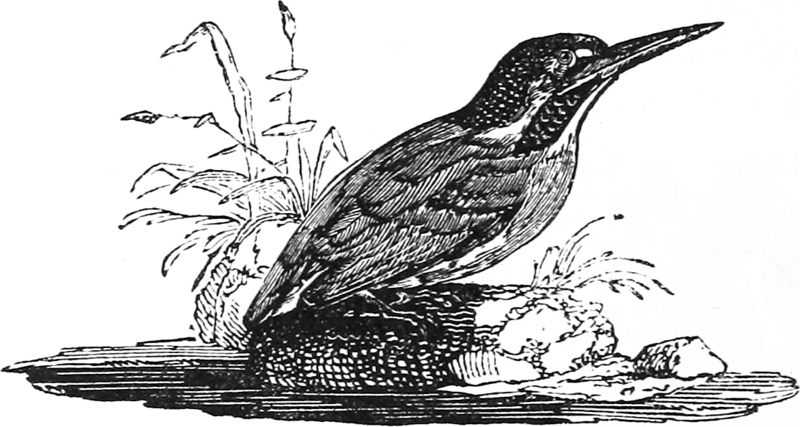
\includegraphics[scale=0.35]{images/Alycon.png}
        \end{figure}
        \vspace{0.5cm}
        \Huge
        \textbf{\textsc{Matematyka Dyskretna}}
        
        \vspace{0.5cm}
        \Large
        \textsc{Wybrane Dowody}
        
        \normalsize
        
        
        \line(1,0){330}
        
        \vspace{1cm}
        \textit{,,Myślę, że 7 punktów na 20 to nie jest zły wynik''}
        \vspace{1cm}

        \textit{\textsc{Popełnione przez}}\\
        \vspace{5mm}

        \textbf{\textsc{Dziurawy Ponton \\ Załatany Ponton \\ Puchaty Pompon \\ Zatopiony Ponton \\ Tonący Ponton \\ Notnop}}

        \vfill

        Kraków \\
        Anno Domini 2023
        
    \end{center}
    
\end{titlepage}


\tableofcontents
\section*{Licencja}
    \begin{figure}[h]
    	\begin{minipage}[c]{0.25\textwidth}
    		
\includegraphics[width=0.7\textwidth]{images/licencja.png}
    	\end{minipage}\hfill
    	\begin{minipage}[c]{0.75\textwidth}
    		\caption*{
    			Ten utwór jest dostępny na 
    			\href{https://creativecommons.org/licenses/by-sa/4.0/}{licencji Creative Commons Uznanie autorstwa
    			na tych samych warunkach 4.0 Międzynarodowe.}
    		}
    	\end{minipage}
    \end{figure}

% Actual content
\mainmatter

\chapter{Kombinatoryka}
 % Żeby nie było syfu to kolejne sekcje dodajemy do chapters/
% A potem includujemy za pomocą \input{chapters/...}

% Używamy \( \) i \[ \] zamiast dolarów -- tak jak się robi w LaTeXu


\documentclass[12pt, a4paper, polish, openany]{book}

% Please, let's familiarize ourselves with notatki.sty and tcs.sty so that we don't reinvent the wheel
\usepackage{notatki}

\fancyhead[L]{\textbf{\textit{MD}}}
\author{
}
\title{TCS and shitposting}


\begin{document}

% Front page and table of contents
\frontmatter

\input{titlepage}

\tableofcontents
\input{license}

% Actual content
\mainmatter

\chapter{Kombinatoryka}
\input{chapters/combinatorics/main}

\chapter{Zasada włączeń i wyłączeń}
\input{chapters/exclusion-inclusion/main}

\chapter{Posety}
\input{chapters/posets/main}

\chapter{Twierdzenie Ramseya}
\input{chapters/ramsey/main}

\chapter{Funkcje tworzące}
\input{chapters/generating_functions/main}

\chapter{Przepływy}
\input{chapters/flows/main}

\chapter{Skojarzenia}
\input{chapters/matchings/main}

\chapter{Kolorowanie grafów}
\input{chapters/graph-coloring/main}

\chapter{Grafy, ale nie kolorowanie}
\input{chapters/graph-misc/main}

\end{document}

\chapter{Zasada włączeń i wyłączeń}
 % Żeby nie było syfu to kolejne sekcje dodajemy do chapters/
% A potem includujemy za pomocą \input{chapters/...}

% Używamy \( \) i \[ \] zamiast dolarów -- tak jak się robi w LaTeXu


\documentclass[12pt, a4paper, polish, openany]{book}

% Please, let's familiarize ourselves with notatki.sty and tcs.sty so that we don't reinvent the wheel
\usepackage{notatki}

\fancyhead[L]{\textbf{\textit{MD}}}
\author{
}
\title{TCS and shitposting}


\begin{document}

% Front page and table of contents
\frontmatter

\input{titlepage}

\tableofcontents
\input{license}

% Actual content
\mainmatter

\chapter{Kombinatoryka}
\input{chapters/combinatorics/main}

\chapter{Zasada włączeń i wyłączeń}
\input{chapters/exclusion-inclusion/main}

\chapter{Posety}
\input{chapters/posets/main}

\chapter{Twierdzenie Ramseya}
\input{chapters/ramsey/main}

\chapter{Funkcje tworzące}
\input{chapters/generating_functions/main}

\chapter{Przepływy}
\input{chapters/flows/main}

\chapter{Skojarzenia}
\input{chapters/matchings/main}

\chapter{Kolorowanie grafów}
\input{chapters/graph-coloring/main}

\chapter{Grafy, ale nie kolorowanie}
\input{chapters/graph-misc/main}

\end{document}

\chapter{Posety}
 % Żeby nie było syfu to kolejne sekcje dodajemy do chapters/
% A potem includujemy za pomocą \input{chapters/...}

% Używamy \( \) i \[ \] zamiast dolarów -- tak jak się robi w LaTeXu


\documentclass[12pt, a4paper, polish, openany]{book}

% Please, let's familiarize ourselves with notatki.sty and tcs.sty so that we don't reinvent the wheel
\usepackage{notatki}

\fancyhead[L]{\textbf{\textit{MD}}}
\author{
}
\title{TCS and shitposting}


\begin{document}

% Front page and table of contents
\frontmatter

\input{titlepage}

\tableofcontents
\input{license}

% Actual content
\mainmatter

\chapter{Kombinatoryka}
\input{chapters/combinatorics/main}

\chapter{Zasada włączeń i wyłączeń}
\input{chapters/exclusion-inclusion/main}

\chapter{Posety}
\input{chapters/posets/main}

\chapter{Twierdzenie Ramseya}
\input{chapters/ramsey/main}

\chapter{Funkcje tworzące}
\input{chapters/generating_functions/main}

\chapter{Przepływy}
\input{chapters/flows/main}

\chapter{Skojarzenia}
\input{chapters/matchings/main}

\chapter{Kolorowanie grafów}
\input{chapters/graph-coloring/main}

\chapter{Grafy, ale nie kolorowanie}
\input{chapters/graph-misc/main}

\end{document}

\chapter{Twierdzenie Ramseya}
 % Żeby nie było syfu to kolejne sekcje dodajemy do chapters/
% A potem includujemy za pomocą \input{chapters/...}

% Używamy \( \) i \[ \] zamiast dolarów -- tak jak się robi w LaTeXu


\documentclass[12pt, a4paper, polish, openany]{book}

% Please, let's familiarize ourselves with notatki.sty and tcs.sty so that we don't reinvent the wheel
\usepackage{notatki}

\fancyhead[L]{\textbf{\textit{MD}}}
\author{
}
\title{TCS and shitposting}


\begin{document}

% Front page and table of contents
\frontmatter

\input{titlepage}

\tableofcontents
\input{license}

% Actual content
\mainmatter

\chapter{Kombinatoryka}
\input{chapters/combinatorics/main}

\chapter{Zasada włączeń i wyłączeń}
\input{chapters/exclusion-inclusion/main}

\chapter{Posety}
\input{chapters/posets/main}

\chapter{Twierdzenie Ramseya}
\input{chapters/ramsey/main}

\chapter{Funkcje tworzące}
\input{chapters/generating_functions/main}

\chapter{Przepływy}
\input{chapters/flows/main}

\chapter{Skojarzenia}
\input{chapters/matchings/main}

\chapter{Kolorowanie grafów}
\input{chapters/graph-coloring/main}

\chapter{Grafy, ale nie kolorowanie}
\input{chapters/graph-misc/main}

\end{document}

\chapter{Funkcje tworzące}
 % Żeby nie było syfu to kolejne sekcje dodajemy do chapters/
% A potem includujemy za pomocą \input{chapters/...}

% Używamy \( \) i \[ \] zamiast dolarów -- tak jak się robi w LaTeXu


\documentclass[12pt, a4paper, polish, openany]{book}

% Please, let's familiarize ourselves with notatki.sty and tcs.sty so that we don't reinvent the wheel
\usepackage{notatki}

\fancyhead[L]{\textbf{\textit{MD}}}
\author{
}
\title{TCS and shitposting}


\begin{document}

% Front page and table of contents
\frontmatter

\input{titlepage}

\tableofcontents
\input{license}

% Actual content
\mainmatter

\chapter{Kombinatoryka}
\input{chapters/combinatorics/main}

\chapter{Zasada włączeń i wyłączeń}
\input{chapters/exclusion-inclusion/main}

\chapter{Posety}
\input{chapters/posets/main}

\chapter{Twierdzenie Ramseya}
\input{chapters/ramsey/main}

\chapter{Funkcje tworzące}
\input{chapters/generating_functions/main}

\chapter{Przepływy}
\input{chapters/flows/main}

\chapter{Skojarzenia}
\input{chapters/matchings/main}

\chapter{Kolorowanie grafów}
\input{chapters/graph-coloring/main}

\chapter{Grafy, ale nie kolorowanie}
\input{chapters/graph-misc/main}

\end{document}

\chapter{Przepływy}
 % Żeby nie było syfu to kolejne sekcje dodajemy do chapters/
% A potem includujemy za pomocą \input{chapters/...}

% Używamy \( \) i \[ \] zamiast dolarów -- tak jak się robi w LaTeXu


\documentclass[12pt, a4paper, polish, openany]{book}

% Please, let's familiarize ourselves with notatki.sty and tcs.sty so that we don't reinvent the wheel
\usepackage{notatki}

\fancyhead[L]{\textbf{\textit{MD}}}
\author{
}
\title{TCS and shitposting}


\begin{document}

% Front page and table of contents
\frontmatter

\input{titlepage}

\tableofcontents
\input{license}

% Actual content
\mainmatter

\chapter{Kombinatoryka}
\input{chapters/combinatorics/main}

\chapter{Zasada włączeń i wyłączeń}
\input{chapters/exclusion-inclusion/main}

\chapter{Posety}
\input{chapters/posets/main}

\chapter{Twierdzenie Ramseya}
\input{chapters/ramsey/main}

\chapter{Funkcje tworzące}
\input{chapters/generating_functions/main}

\chapter{Przepływy}
\input{chapters/flows/main}

\chapter{Skojarzenia}
\input{chapters/matchings/main}

\chapter{Kolorowanie grafów}
\input{chapters/graph-coloring/main}

\chapter{Grafy, ale nie kolorowanie}
\input{chapters/graph-misc/main}

\end{document}

\chapter{Skojarzenia}
 % Żeby nie było syfu to kolejne sekcje dodajemy do chapters/
% A potem includujemy za pomocą \input{chapters/...}

% Używamy \( \) i \[ \] zamiast dolarów -- tak jak się robi w LaTeXu


\documentclass[12pt, a4paper, polish, openany]{book}

% Please, let's familiarize ourselves with notatki.sty and tcs.sty so that we don't reinvent the wheel
\usepackage{notatki}

\fancyhead[L]{\textbf{\textit{MD}}}
\author{
}
\title{TCS and shitposting}


\begin{document}

% Front page and table of contents
\frontmatter

\input{titlepage}

\tableofcontents
\input{license}

% Actual content
\mainmatter

\chapter{Kombinatoryka}
\input{chapters/combinatorics/main}

\chapter{Zasada włączeń i wyłączeń}
\input{chapters/exclusion-inclusion/main}

\chapter{Posety}
\input{chapters/posets/main}

\chapter{Twierdzenie Ramseya}
\input{chapters/ramsey/main}

\chapter{Funkcje tworzące}
\input{chapters/generating_functions/main}

\chapter{Przepływy}
\input{chapters/flows/main}

\chapter{Skojarzenia}
\input{chapters/matchings/main}

\chapter{Kolorowanie grafów}
\input{chapters/graph-coloring/main}

\chapter{Grafy, ale nie kolorowanie}
\input{chapters/graph-misc/main}

\end{document}

\chapter{Kolorowanie grafów}
 % Żeby nie było syfu to kolejne sekcje dodajemy do chapters/
% A potem includujemy za pomocą \input{chapters/...}

% Używamy \( \) i \[ \] zamiast dolarów -- tak jak się robi w LaTeXu


\documentclass[12pt, a4paper, polish, openany]{book}

% Please, let's familiarize ourselves with notatki.sty and tcs.sty so that we don't reinvent the wheel
\usepackage{notatki}

\fancyhead[L]{\textbf{\textit{MD}}}
\author{
}
\title{TCS and shitposting}


\begin{document}

% Front page and table of contents
\frontmatter

\input{titlepage}

\tableofcontents
\input{license}

% Actual content
\mainmatter

\chapter{Kombinatoryka}
\input{chapters/combinatorics/main}

\chapter{Zasada włączeń i wyłączeń}
\input{chapters/exclusion-inclusion/main}

\chapter{Posety}
\input{chapters/posets/main}

\chapter{Twierdzenie Ramseya}
\input{chapters/ramsey/main}

\chapter{Funkcje tworzące}
\input{chapters/generating_functions/main}

\chapter{Przepływy}
\input{chapters/flows/main}

\chapter{Skojarzenia}
\input{chapters/matchings/main}

\chapter{Kolorowanie grafów}
\input{chapters/graph-coloring/main}

\chapter{Grafy, ale nie kolorowanie}
\input{chapters/graph-misc/main}

\end{document}

\chapter{Grafy, ale nie kolorowanie}
 % Żeby nie było syfu to kolejne sekcje dodajemy do chapters/
% A potem includujemy za pomocą \input{chapters/...}

% Używamy \( \) i \[ \] zamiast dolarów -- tak jak się robi w LaTeXu


\documentclass[12pt, a4paper, polish, openany]{book}

% Please, let's familiarize ourselves with notatki.sty and tcs.sty so that we don't reinvent the wheel
\usepackage{notatki}

\fancyhead[L]{\textbf{\textit{MD}}}
\author{
}
\title{TCS and shitposting}


\begin{document}

% Front page and table of contents
\frontmatter

\input{titlepage}

\tableofcontents
\input{license}

% Actual content
\mainmatter

\chapter{Kombinatoryka}
\input{chapters/combinatorics/main}

\chapter{Zasada włączeń i wyłączeń}
\input{chapters/exclusion-inclusion/main}

\chapter{Posety}
\input{chapters/posets/main}

\chapter{Twierdzenie Ramseya}
\input{chapters/ramsey/main}

\chapter{Funkcje tworzące}
\input{chapters/generating_functions/main}

\chapter{Przepływy}
\input{chapters/flows/main}

\chapter{Skojarzenia}
\input{chapters/matchings/main}

\chapter{Kolorowanie grafów}
\input{chapters/graph-coloring/main}

\chapter{Grafy, ale nie kolorowanie}
\input{chapters/graph-misc/main}

\end{document}

\end{document}

\chapter{Funkcje tworzące}
 % Żeby nie było syfu to kolejne sekcje dodajemy do chapters/
% A potem includujemy za pomocą \input{chapters/...}

% Używamy \( \) i \[ \] zamiast dolarów -- tak jak się robi w LaTeXu


\documentclass[12pt, a4paper, polish, openany]{book}

% Please, let's familiarize ourselves with notatki.sty and tcs.sty so that we don't reinvent the wheel
\usepackage{notatki}

\fancyhead[L]{\textbf{\textit{MD}}}
\author{
}
\title{TCS and shitposting}


\begin{document}

% Front page and table of contents
\frontmatter

\begin{titlepage} 

    \begin{center}
         \begin{figure}[h]
            \centering
            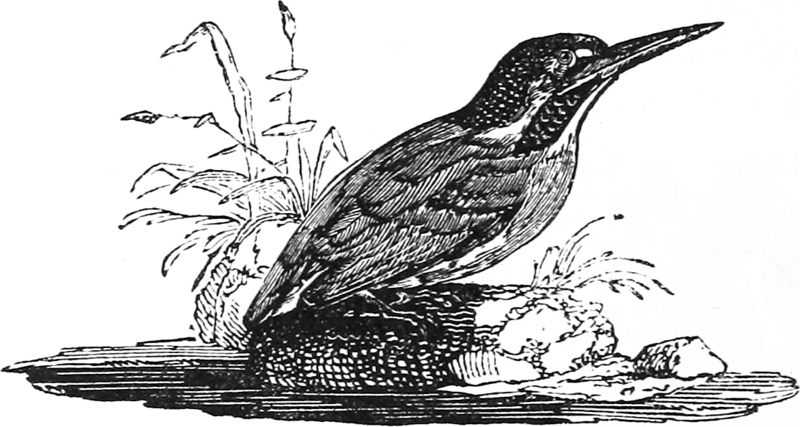
\includegraphics[scale=0.35]{images/Alycon.png}
        \end{figure}
        \vspace{0.5cm}
        \Huge
        \textbf{\textsc{Matematyka Dyskretna}}
        
        \vspace{0.5cm}
        \Large
        \textsc{Wybrane Dowody}
        
        \normalsize
        
        
        \line(1,0){330}
        
        \vspace{1cm}
        \textit{,,Myślę, że 7 punktów na 20 to nie jest zły wynik''}
        \vspace{1cm}

        \textit{\textsc{Popełnione przez}}\\
        \vspace{5mm}

        \textbf{\textsc{Dziurawy Ponton \\ Załatany Ponton \\ Puchaty Pompon \\ Zatopiony Ponton \\ Tonący Ponton \\ Notnop}}

        \vfill

        Kraków \\
        Anno Domini 2023
        
    \end{center}
    
\end{titlepage}


\tableofcontents
\section*{Licencja}
    \begin{figure}[h]
    	\begin{minipage}[c]{0.25\textwidth}
    		
\includegraphics[width=0.7\textwidth]{images/licencja.png}
    	\end{minipage}\hfill
    	\begin{minipage}[c]{0.75\textwidth}
    		\caption*{
    			Ten utwór jest dostępny na 
    			\href{https://creativecommons.org/licenses/by-sa/4.0/}{licencji Creative Commons Uznanie autorstwa
    			na tych samych warunkach 4.0 Międzynarodowe.}
    		}
    	\end{minipage}
    \end{figure}

% Actual content
\mainmatter

\chapter{Kombinatoryka}
 % Żeby nie było syfu to kolejne sekcje dodajemy do chapters/
% A potem includujemy za pomocą \input{chapters/...}

% Używamy \( \) i \[ \] zamiast dolarów -- tak jak się robi w LaTeXu


\documentclass[12pt, a4paper, polish, openany]{book}

% Please, let's familiarize ourselves with notatki.sty and tcs.sty so that we don't reinvent the wheel
\usepackage{notatki}

\fancyhead[L]{\textbf{\textit{MD}}}
\author{
}
\title{TCS and shitposting}


\begin{document}

% Front page and table of contents
\frontmatter

\input{titlepage}

\tableofcontents
\input{license}

% Actual content
\mainmatter

\chapter{Kombinatoryka}
\input{chapters/combinatorics/main}

\chapter{Zasada włączeń i wyłączeń}
\input{chapters/exclusion-inclusion/main}

\chapter{Posety}
\input{chapters/posets/main}

\chapter{Twierdzenie Ramseya}
\input{chapters/ramsey/main}

\chapter{Funkcje tworzące}
\input{chapters/generating_functions/main}

\chapter{Przepływy}
\input{chapters/flows/main}

\chapter{Skojarzenia}
\input{chapters/matchings/main}

\chapter{Kolorowanie grafów}
\input{chapters/graph-coloring/main}

\chapter{Grafy, ale nie kolorowanie}
\input{chapters/graph-misc/main}

\end{document}

\chapter{Zasada włączeń i wyłączeń}
 % Żeby nie było syfu to kolejne sekcje dodajemy do chapters/
% A potem includujemy za pomocą \input{chapters/...}

% Używamy \( \) i \[ \] zamiast dolarów -- tak jak się robi w LaTeXu


\documentclass[12pt, a4paper, polish, openany]{book}

% Please, let's familiarize ourselves with notatki.sty and tcs.sty so that we don't reinvent the wheel
\usepackage{notatki}

\fancyhead[L]{\textbf{\textit{MD}}}
\author{
}
\title{TCS and shitposting}


\begin{document}

% Front page and table of contents
\frontmatter

\input{titlepage}

\tableofcontents
\input{license}

% Actual content
\mainmatter

\chapter{Kombinatoryka}
\input{chapters/combinatorics/main}

\chapter{Zasada włączeń i wyłączeń}
\input{chapters/exclusion-inclusion/main}

\chapter{Posety}
\input{chapters/posets/main}

\chapter{Twierdzenie Ramseya}
\input{chapters/ramsey/main}

\chapter{Funkcje tworzące}
\input{chapters/generating_functions/main}

\chapter{Przepływy}
\input{chapters/flows/main}

\chapter{Skojarzenia}
\input{chapters/matchings/main}

\chapter{Kolorowanie grafów}
\input{chapters/graph-coloring/main}

\chapter{Grafy, ale nie kolorowanie}
\input{chapters/graph-misc/main}

\end{document}

\chapter{Posety}
 % Żeby nie było syfu to kolejne sekcje dodajemy do chapters/
% A potem includujemy za pomocą \input{chapters/...}

% Używamy \( \) i \[ \] zamiast dolarów -- tak jak się robi w LaTeXu


\documentclass[12pt, a4paper, polish, openany]{book}

% Please, let's familiarize ourselves with notatki.sty and tcs.sty so that we don't reinvent the wheel
\usepackage{notatki}

\fancyhead[L]{\textbf{\textit{MD}}}
\author{
}
\title{TCS and shitposting}


\begin{document}

% Front page and table of contents
\frontmatter

\input{titlepage}

\tableofcontents
\input{license}

% Actual content
\mainmatter

\chapter{Kombinatoryka}
\input{chapters/combinatorics/main}

\chapter{Zasada włączeń i wyłączeń}
\input{chapters/exclusion-inclusion/main}

\chapter{Posety}
\input{chapters/posets/main}

\chapter{Twierdzenie Ramseya}
\input{chapters/ramsey/main}

\chapter{Funkcje tworzące}
\input{chapters/generating_functions/main}

\chapter{Przepływy}
\input{chapters/flows/main}

\chapter{Skojarzenia}
\input{chapters/matchings/main}

\chapter{Kolorowanie grafów}
\input{chapters/graph-coloring/main}

\chapter{Grafy, ale nie kolorowanie}
\input{chapters/graph-misc/main}

\end{document}

\chapter{Twierdzenie Ramseya}
 % Żeby nie było syfu to kolejne sekcje dodajemy do chapters/
% A potem includujemy za pomocą \input{chapters/...}

% Używamy \( \) i \[ \] zamiast dolarów -- tak jak się robi w LaTeXu


\documentclass[12pt, a4paper, polish, openany]{book}

% Please, let's familiarize ourselves with notatki.sty and tcs.sty so that we don't reinvent the wheel
\usepackage{notatki}

\fancyhead[L]{\textbf{\textit{MD}}}
\author{
}
\title{TCS and shitposting}


\begin{document}

% Front page and table of contents
\frontmatter

\input{titlepage}

\tableofcontents
\input{license}

% Actual content
\mainmatter

\chapter{Kombinatoryka}
\input{chapters/combinatorics/main}

\chapter{Zasada włączeń i wyłączeń}
\input{chapters/exclusion-inclusion/main}

\chapter{Posety}
\input{chapters/posets/main}

\chapter{Twierdzenie Ramseya}
\input{chapters/ramsey/main}

\chapter{Funkcje tworzące}
\input{chapters/generating_functions/main}

\chapter{Przepływy}
\input{chapters/flows/main}

\chapter{Skojarzenia}
\input{chapters/matchings/main}

\chapter{Kolorowanie grafów}
\input{chapters/graph-coloring/main}

\chapter{Grafy, ale nie kolorowanie}
\input{chapters/graph-misc/main}

\end{document}

\chapter{Funkcje tworzące}
 % Żeby nie było syfu to kolejne sekcje dodajemy do chapters/
% A potem includujemy za pomocą \input{chapters/...}

% Używamy \( \) i \[ \] zamiast dolarów -- tak jak się robi w LaTeXu


\documentclass[12pt, a4paper, polish, openany]{book}

% Please, let's familiarize ourselves with notatki.sty and tcs.sty so that we don't reinvent the wheel
\usepackage{notatki}

\fancyhead[L]{\textbf{\textit{MD}}}
\author{
}
\title{TCS and shitposting}


\begin{document}

% Front page and table of contents
\frontmatter

\input{titlepage}

\tableofcontents
\input{license}

% Actual content
\mainmatter

\chapter{Kombinatoryka}
\input{chapters/combinatorics/main}

\chapter{Zasada włączeń i wyłączeń}
\input{chapters/exclusion-inclusion/main}

\chapter{Posety}
\input{chapters/posets/main}

\chapter{Twierdzenie Ramseya}
\input{chapters/ramsey/main}

\chapter{Funkcje tworzące}
\input{chapters/generating_functions/main}

\chapter{Przepływy}
\input{chapters/flows/main}

\chapter{Skojarzenia}
\input{chapters/matchings/main}

\chapter{Kolorowanie grafów}
\input{chapters/graph-coloring/main}

\chapter{Grafy, ale nie kolorowanie}
\input{chapters/graph-misc/main}

\end{document}

\chapter{Przepływy}
 % Żeby nie było syfu to kolejne sekcje dodajemy do chapters/
% A potem includujemy za pomocą \input{chapters/...}

% Używamy \( \) i \[ \] zamiast dolarów -- tak jak się robi w LaTeXu


\documentclass[12pt, a4paper, polish, openany]{book}

% Please, let's familiarize ourselves with notatki.sty and tcs.sty so that we don't reinvent the wheel
\usepackage{notatki}

\fancyhead[L]{\textbf{\textit{MD}}}
\author{
}
\title{TCS and shitposting}


\begin{document}

% Front page and table of contents
\frontmatter

\input{titlepage}

\tableofcontents
\input{license}

% Actual content
\mainmatter

\chapter{Kombinatoryka}
\input{chapters/combinatorics/main}

\chapter{Zasada włączeń i wyłączeń}
\input{chapters/exclusion-inclusion/main}

\chapter{Posety}
\input{chapters/posets/main}

\chapter{Twierdzenie Ramseya}
\input{chapters/ramsey/main}

\chapter{Funkcje tworzące}
\input{chapters/generating_functions/main}

\chapter{Przepływy}
\input{chapters/flows/main}

\chapter{Skojarzenia}
\input{chapters/matchings/main}

\chapter{Kolorowanie grafów}
\input{chapters/graph-coloring/main}

\chapter{Grafy, ale nie kolorowanie}
\input{chapters/graph-misc/main}

\end{document}

\chapter{Skojarzenia}
 % Żeby nie było syfu to kolejne sekcje dodajemy do chapters/
% A potem includujemy za pomocą \input{chapters/...}

% Używamy \( \) i \[ \] zamiast dolarów -- tak jak się robi w LaTeXu


\documentclass[12pt, a4paper, polish, openany]{book}

% Please, let's familiarize ourselves with notatki.sty and tcs.sty so that we don't reinvent the wheel
\usepackage{notatki}

\fancyhead[L]{\textbf{\textit{MD}}}
\author{
}
\title{TCS and shitposting}


\begin{document}

% Front page and table of contents
\frontmatter

\input{titlepage}

\tableofcontents
\input{license}

% Actual content
\mainmatter

\chapter{Kombinatoryka}
\input{chapters/combinatorics/main}

\chapter{Zasada włączeń i wyłączeń}
\input{chapters/exclusion-inclusion/main}

\chapter{Posety}
\input{chapters/posets/main}

\chapter{Twierdzenie Ramseya}
\input{chapters/ramsey/main}

\chapter{Funkcje tworzące}
\input{chapters/generating_functions/main}

\chapter{Przepływy}
\input{chapters/flows/main}

\chapter{Skojarzenia}
\input{chapters/matchings/main}

\chapter{Kolorowanie grafów}
\input{chapters/graph-coloring/main}

\chapter{Grafy, ale nie kolorowanie}
\input{chapters/graph-misc/main}

\end{document}

\chapter{Kolorowanie grafów}
 % Żeby nie było syfu to kolejne sekcje dodajemy do chapters/
% A potem includujemy za pomocą \input{chapters/...}

% Używamy \( \) i \[ \] zamiast dolarów -- tak jak się robi w LaTeXu


\documentclass[12pt, a4paper, polish, openany]{book}

% Please, let's familiarize ourselves with notatki.sty and tcs.sty so that we don't reinvent the wheel
\usepackage{notatki}

\fancyhead[L]{\textbf{\textit{MD}}}
\author{
}
\title{TCS and shitposting}


\begin{document}

% Front page and table of contents
\frontmatter

\input{titlepage}

\tableofcontents
\input{license}

% Actual content
\mainmatter

\chapter{Kombinatoryka}
\input{chapters/combinatorics/main}

\chapter{Zasada włączeń i wyłączeń}
\input{chapters/exclusion-inclusion/main}

\chapter{Posety}
\input{chapters/posets/main}

\chapter{Twierdzenie Ramseya}
\input{chapters/ramsey/main}

\chapter{Funkcje tworzące}
\input{chapters/generating_functions/main}

\chapter{Przepływy}
\input{chapters/flows/main}

\chapter{Skojarzenia}
\input{chapters/matchings/main}

\chapter{Kolorowanie grafów}
\input{chapters/graph-coloring/main}

\chapter{Grafy, ale nie kolorowanie}
\input{chapters/graph-misc/main}

\end{document}

\chapter{Grafy, ale nie kolorowanie}
 % Żeby nie było syfu to kolejne sekcje dodajemy do chapters/
% A potem includujemy za pomocą \input{chapters/...}

% Używamy \( \) i \[ \] zamiast dolarów -- tak jak się robi w LaTeXu


\documentclass[12pt, a4paper, polish, openany]{book}

% Please, let's familiarize ourselves with notatki.sty and tcs.sty so that we don't reinvent the wheel
\usepackage{notatki}

\fancyhead[L]{\textbf{\textit{MD}}}
\author{
}
\title{TCS and shitposting}


\begin{document}

% Front page and table of contents
\frontmatter

\input{titlepage}

\tableofcontents
\input{license}

% Actual content
\mainmatter

\chapter{Kombinatoryka}
\input{chapters/combinatorics/main}

\chapter{Zasada włączeń i wyłączeń}
\input{chapters/exclusion-inclusion/main}

\chapter{Posety}
\input{chapters/posets/main}

\chapter{Twierdzenie Ramseya}
\input{chapters/ramsey/main}

\chapter{Funkcje tworzące}
\input{chapters/generating_functions/main}

\chapter{Przepływy}
\input{chapters/flows/main}

\chapter{Skojarzenia}
\input{chapters/matchings/main}

\chapter{Kolorowanie grafów}
\input{chapters/graph-coloring/main}

\chapter{Grafy, ale nie kolorowanie}
\input{chapters/graph-misc/main}

\end{document}

\end{document}

\chapter{Przepływy}
 % Żeby nie było syfu to kolejne sekcje dodajemy do chapters/
% A potem includujemy za pomocą \input{chapters/...}

% Używamy \( \) i \[ \] zamiast dolarów -- tak jak się robi w LaTeXu


\documentclass[12pt, a4paper, polish, openany]{book}

% Please, let's familiarize ourselves with notatki.sty and tcs.sty so that we don't reinvent the wheel
\usepackage{notatki}

\fancyhead[L]{\textbf{\textit{MD}}}
\author{
}
\title{TCS and shitposting}


\begin{document}

% Front page and table of contents
\frontmatter

\begin{titlepage} 

    \begin{center}
         \begin{figure}[h]
            \centering
            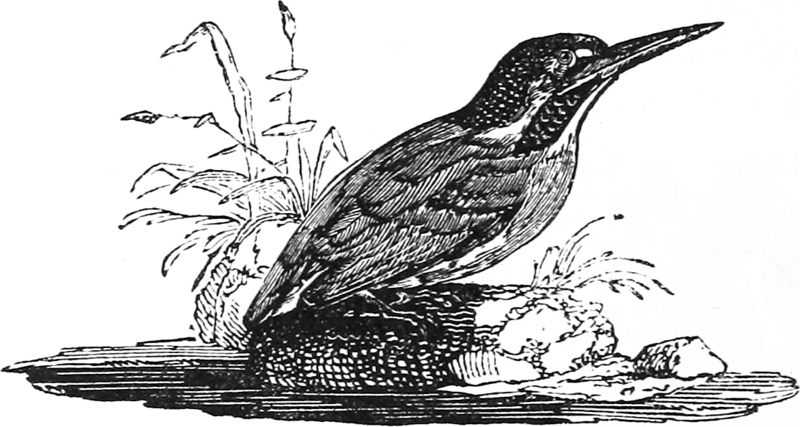
\includegraphics[scale=0.35]{images/Alycon.png}
        \end{figure}
        \vspace{0.5cm}
        \Huge
        \textbf{\textsc{Matematyka Dyskretna}}
        
        \vspace{0.5cm}
        \Large
        \textsc{Wybrane Dowody}
        
        \normalsize
        
        
        \line(1,0){330}
        
        \vspace{1cm}
        \textit{,,Myślę, że 7 punktów na 20 to nie jest zły wynik''}
        \vspace{1cm}

        \textit{\textsc{Popełnione przez}}\\
        \vspace{5mm}

        \textbf{\textsc{Dziurawy Ponton \\ Załatany Ponton \\ Puchaty Pompon \\ Zatopiony Ponton \\ Tonący Ponton \\ Notnop}}

        \vfill

        Kraków \\
        Anno Domini 2023
        
    \end{center}
    
\end{titlepage}


\tableofcontents
\section*{Licencja}
    \begin{figure}[h]
    	\begin{minipage}[c]{0.25\textwidth}
    		
\includegraphics[width=0.7\textwidth]{images/licencja.png}
    	\end{minipage}\hfill
    	\begin{minipage}[c]{0.75\textwidth}
    		\caption*{
    			Ten utwór jest dostępny na 
    			\href{https://creativecommons.org/licenses/by-sa/4.0/}{licencji Creative Commons Uznanie autorstwa
    			na tych samych warunkach 4.0 Międzynarodowe.}
    		}
    	\end{minipage}
    \end{figure}

% Actual content
\mainmatter

\chapter{Kombinatoryka}
 % Żeby nie było syfu to kolejne sekcje dodajemy do chapters/
% A potem includujemy za pomocą \input{chapters/...}

% Używamy \( \) i \[ \] zamiast dolarów -- tak jak się robi w LaTeXu


\documentclass[12pt, a4paper, polish, openany]{book}

% Please, let's familiarize ourselves with notatki.sty and tcs.sty so that we don't reinvent the wheel
\usepackage{notatki}

\fancyhead[L]{\textbf{\textit{MD}}}
\author{
}
\title{TCS and shitposting}


\begin{document}

% Front page and table of contents
\frontmatter

\input{titlepage}

\tableofcontents
\input{license}

% Actual content
\mainmatter

\chapter{Kombinatoryka}
\input{chapters/combinatorics/main}

\chapter{Zasada włączeń i wyłączeń}
\input{chapters/exclusion-inclusion/main}

\chapter{Posety}
\input{chapters/posets/main}

\chapter{Twierdzenie Ramseya}
\input{chapters/ramsey/main}

\chapter{Funkcje tworzące}
\input{chapters/generating_functions/main}

\chapter{Przepływy}
\input{chapters/flows/main}

\chapter{Skojarzenia}
\input{chapters/matchings/main}

\chapter{Kolorowanie grafów}
\input{chapters/graph-coloring/main}

\chapter{Grafy, ale nie kolorowanie}
\input{chapters/graph-misc/main}

\end{document}

\chapter{Zasada włączeń i wyłączeń}
 % Żeby nie było syfu to kolejne sekcje dodajemy do chapters/
% A potem includujemy za pomocą \input{chapters/...}

% Używamy \( \) i \[ \] zamiast dolarów -- tak jak się robi w LaTeXu


\documentclass[12pt, a4paper, polish, openany]{book}

% Please, let's familiarize ourselves with notatki.sty and tcs.sty so that we don't reinvent the wheel
\usepackage{notatki}

\fancyhead[L]{\textbf{\textit{MD}}}
\author{
}
\title{TCS and shitposting}


\begin{document}

% Front page and table of contents
\frontmatter

\input{titlepage}

\tableofcontents
\input{license}

% Actual content
\mainmatter

\chapter{Kombinatoryka}
\input{chapters/combinatorics/main}

\chapter{Zasada włączeń i wyłączeń}
\input{chapters/exclusion-inclusion/main}

\chapter{Posety}
\input{chapters/posets/main}

\chapter{Twierdzenie Ramseya}
\input{chapters/ramsey/main}

\chapter{Funkcje tworzące}
\input{chapters/generating_functions/main}

\chapter{Przepływy}
\input{chapters/flows/main}

\chapter{Skojarzenia}
\input{chapters/matchings/main}

\chapter{Kolorowanie grafów}
\input{chapters/graph-coloring/main}

\chapter{Grafy, ale nie kolorowanie}
\input{chapters/graph-misc/main}

\end{document}

\chapter{Posety}
 % Żeby nie było syfu to kolejne sekcje dodajemy do chapters/
% A potem includujemy za pomocą \input{chapters/...}

% Używamy \( \) i \[ \] zamiast dolarów -- tak jak się robi w LaTeXu


\documentclass[12pt, a4paper, polish, openany]{book}

% Please, let's familiarize ourselves with notatki.sty and tcs.sty so that we don't reinvent the wheel
\usepackage{notatki}

\fancyhead[L]{\textbf{\textit{MD}}}
\author{
}
\title{TCS and shitposting}


\begin{document}

% Front page and table of contents
\frontmatter

\input{titlepage}

\tableofcontents
\input{license}

% Actual content
\mainmatter

\chapter{Kombinatoryka}
\input{chapters/combinatorics/main}

\chapter{Zasada włączeń i wyłączeń}
\input{chapters/exclusion-inclusion/main}

\chapter{Posety}
\input{chapters/posets/main}

\chapter{Twierdzenie Ramseya}
\input{chapters/ramsey/main}

\chapter{Funkcje tworzące}
\input{chapters/generating_functions/main}

\chapter{Przepływy}
\input{chapters/flows/main}

\chapter{Skojarzenia}
\input{chapters/matchings/main}

\chapter{Kolorowanie grafów}
\input{chapters/graph-coloring/main}

\chapter{Grafy, ale nie kolorowanie}
\input{chapters/graph-misc/main}

\end{document}

\chapter{Twierdzenie Ramseya}
 % Żeby nie było syfu to kolejne sekcje dodajemy do chapters/
% A potem includujemy za pomocą \input{chapters/...}

% Używamy \( \) i \[ \] zamiast dolarów -- tak jak się robi w LaTeXu


\documentclass[12pt, a4paper, polish, openany]{book}

% Please, let's familiarize ourselves with notatki.sty and tcs.sty so that we don't reinvent the wheel
\usepackage{notatki}

\fancyhead[L]{\textbf{\textit{MD}}}
\author{
}
\title{TCS and shitposting}


\begin{document}

% Front page and table of contents
\frontmatter

\input{titlepage}

\tableofcontents
\input{license}

% Actual content
\mainmatter

\chapter{Kombinatoryka}
\input{chapters/combinatorics/main}

\chapter{Zasada włączeń i wyłączeń}
\input{chapters/exclusion-inclusion/main}

\chapter{Posety}
\input{chapters/posets/main}

\chapter{Twierdzenie Ramseya}
\input{chapters/ramsey/main}

\chapter{Funkcje tworzące}
\input{chapters/generating_functions/main}

\chapter{Przepływy}
\input{chapters/flows/main}

\chapter{Skojarzenia}
\input{chapters/matchings/main}

\chapter{Kolorowanie grafów}
\input{chapters/graph-coloring/main}

\chapter{Grafy, ale nie kolorowanie}
\input{chapters/graph-misc/main}

\end{document}

\chapter{Funkcje tworzące}
 % Żeby nie było syfu to kolejne sekcje dodajemy do chapters/
% A potem includujemy za pomocą \input{chapters/...}

% Używamy \( \) i \[ \] zamiast dolarów -- tak jak się robi w LaTeXu


\documentclass[12pt, a4paper, polish, openany]{book}

% Please, let's familiarize ourselves with notatki.sty and tcs.sty so that we don't reinvent the wheel
\usepackage{notatki}

\fancyhead[L]{\textbf{\textit{MD}}}
\author{
}
\title{TCS and shitposting}


\begin{document}

% Front page and table of contents
\frontmatter

\input{titlepage}

\tableofcontents
\input{license}

% Actual content
\mainmatter

\chapter{Kombinatoryka}
\input{chapters/combinatorics/main}

\chapter{Zasada włączeń i wyłączeń}
\input{chapters/exclusion-inclusion/main}

\chapter{Posety}
\input{chapters/posets/main}

\chapter{Twierdzenie Ramseya}
\input{chapters/ramsey/main}

\chapter{Funkcje tworzące}
\input{chapters/generating_functions/main}

\chapter{Przepływy}
\input{chapters/flows/main}

\chapter{Skojarzenia}
\input{chapters/matchings/main}

\chapter{Kolorowanie grafów}
\input{chapters/graph-coloring/main}

\chapter{Grafy, ale nie kolorowanie}
\input{chapters/graph-misc/main}

\end{document}

\chapter{Przepływy}
 % Żeby nie było syfu to kolejne sekcje dodajemy do chapters/
% A potem includujemy za pomocą \input{chapters/...}

% Używamy \( \) i \[ \] zamiast dolarów -- tak jak się robi w LaTeXu


\documentclass[12pt, a4paper, polish, openany]{book}

% Please, let's familiarize ourselves with notatki.sty and tcs.sty so that we don't reinvent the wheel
\usepackage{notatki}

\fancyhead[L]{\textbf{\textit{MD}}}
\author{
}
\title{TCS and shitposting}


\begin{document}

% Front page and table of contents
\frontmatter

\input{titlepage}

\tableofcontents
\input{license}

% Actual content
\mainmatter

\chapter{Kombinatoryka}
\input{chapters/combinatorics/main}

\chapter{Zasada włączeń i wyłączeń}
\input{chapters/exclusion-inclusion/main}

\chapter{Posety}
\input{chapters/posets/main}

\chapter{Twierdzenie Ramseya}
\input{chapters/ramsey/main}

\chapter{Funkcje tworzące}
\input{chapters/generating_functions/main}

\chapter{Przepływy}
\input{chapters/flows/main}

\chapter{Skojarzenia}
\input{chapters/matchings/main}

\chapter{Kolorowanie grafów}
\input{chapters/graph-coloring/main}

\chapter{Grafy, ale nie kolorowanie}
\input{chapters/graph-misc/main}

\end{document}

\chapter{Skojarzenia}
 % Żeby nie było syfu to kolejne sekcje dodajemy do chapters/
% A potem includujemy za pomocą \input{chapters/...}

% Używamy \( \) i \[ \] zamiast dolarów -- tak jak się robi w LaTeXu


\documentclass[12pt, a4paper, polish, openany]{book}

% Please, let's familiarize ourselves with notatki.sty and tcs.sty so that we don't reinvent the wheel
\usepackage{notatki}

\fancyhead[L]{\textbf{\textit{MD}}}
\author{
}
\title{TCS and shitposting}


\begin{document}

% Front page and table of contents
\frontmatter

\input{titlepage}

\tableofcontents
\input{license}

% Actual content
\mainmatter

\chapter{Kombinatoryka}
\input{chapters/combinatorics/main}

\chapter{Zasada włączeń i wyłączeń}
\input{chapters/exclusion-inclusion/main}

\chapter{Posety}
\input{chapters/posets/main}

\chapter{Twierdzenie Ramseya}
\input{chapters/ramsey/main}

\chapter{Funkcje tworzące}
\input{chapters/generating_functions/main}

\chapter{Przepływy}
\input{chapters/flows/main}

\chapter{Skojarzenia}
\input{chapters/matchings/main}

\chapter{Kolorowanie grafów}
\input{chapters/graph-coloring/main}

\chapter{Grafy, ale nie kolorowanie}
\input{chapters/graph-misc/main}

\end{document}

\chapter{Kolorowanie grafów}
 % Żeby nie było syfu to kolejne sekcje dodajemy do chapters/
% A potem includujemy za pomocą \input{chapters/...}

% Używamy \( \) i \[ \] zamiast dolarów -- tak jak się robi w LaTeXu


\documentclass[12pt, a4paper, polish, openany]{book}

% Please, let's familiarize ourselves with notatki.sty and tcs.sty so that we don't reinvent the wheel
\usepackage{notatki}

\fancyhead[L]{\textbf{\textit{MD}}}
\author{
}
\title{TCS and shitposting}


\begin{document}

% Front page and table of contents
\frontmatter

\input{titlepage}

\tableofcontents
\input{license}

% Actual content
\mainmatter

\chapter{Kombinatoryka}
\input{chapters/combinatorics/main}

\chapter{Zasada włączeń i wyłączeń}
\input{chapters/exclusion-inclusion/main}

\chapter{Posety}
\input{chapters/posets/main}

\chapter{Twierdzenie Ramseya}
\input{chapters/ramsey/main}

\chapter{Funkcje tworzące}
\input{chapters/generating_functions/main}

\chapter{Przepływy}
\input{chapters/flows/main}

\chapter{Skojarzenia}
\input{chapters/matchings/main}

\chapter{Kolorowanie grafów}
\input{chapters/graph-coloring/main}

\chapter{Grafy, ale nie kolorowanie}
\input{chapters/graph-misc/main}

\end{document}

\chapter{Grafy, ale nie kolorowanie}
 % Żeby nie było syfu to kolejne sekcje dodajemy do chapters/
% A potem includujemy za pomocą \input{chapters/...}

% Używamy \( \) i \[ \] zamiast dolarów -- tak jak się robi w LaTeXu


\documentclass[12pt, a4paper, polish, openany]{book}

% Please, let's familiarize ourselves with notatki.sty and tcs.sty so that we don't reinvent the wheel
\usepackage{notatki}

\fancyhead[L]{\textbf{\textit{MD}}}
\author{
}
\title{TCS and shitposting}


\begin{document}

% Front page and table of contents
\frontmatter

\input{titlepage}

\tableofcontents
\input{license}

% Actual content
\mainmatter

\chapter{Kombinatoryka}
\input{chapters/combinatorics/main}

\chapter{Zasada włączeń i wyłączeń}
\input{chapters/exclusion-inclusion/main}

\chapter{Posety}
\input{chapters/posets/main}

\chapter{Twierdzenie Ramseya}
\input{chapters/ramsey/main}

\chapter{Funkcje tworzące}
\input{chapters/generating_functions/main}

\chapter{Przepływy}
\input{chapters/flows/main}

\chapter{Skojarzenia}
\input{chapters/matchings/main}

\chapter{Kolorowanie grafów}
\input{chapters/graph-coloring/main}

\chapter{Grafy, ale nie kolorowanie}
\input{chapters/graph-misc/main}

\end{document}

\end{document}

\chapter{Skojarzenia}
 % Żeby nie było syfu to kolejne sekcje dodajemy do chapters/
% A potem includujemy za pomocą \input{chapters/...}

% Używamy \( \) i \[ \] zamiast dolarów -- tak jak się robi w LaTeXu


\documentclass[12pt, a4paper, polish, openany]{book}

% Please, let's familiarize ourselves with notatki.sty and tcs.sty so that we don't reinvent the wheel
\usepackage{notatki}

\fancyhead[L]{\textbf{\textit{MD}}}
\author{
}
\title{TCS and shitposting}


\begin{document}

% Front page and table of contents
\frontmatter

\begin{titlepage} 

    \begin{center}
         \begin{figure}[h]
            \centering
            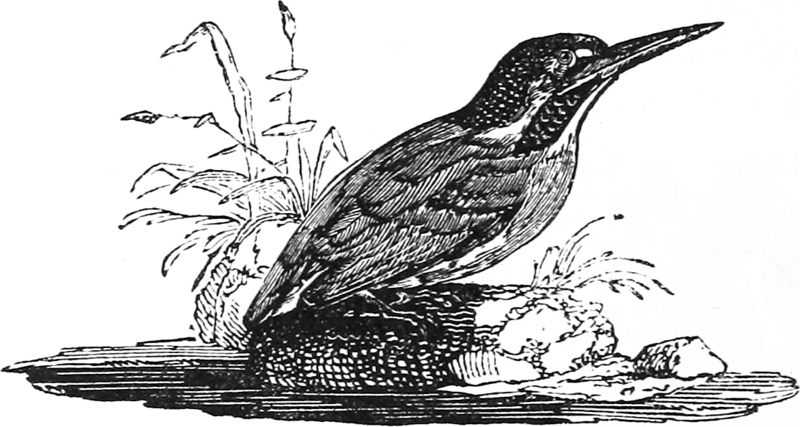
\includegraphics[scale=0.35]{images/Alycon.png}
        \end{figure}
        \vspace{0.5cm}
        \Huge
        \textbf{\textsc{Matematyka Dyskretna}}
        
        \vspace{0.5cm}
        \Large
        \textsc{Wybrane Dowody}
        
        \normalsize
        
        
        \line(1,0){330}
        
        \vspace{1cm}
        \textit{,,Myślę, że 7 punktów na 20 to nie jest zły wynik''}
        \vspace{1cm}

        \textit{\textsc{Popełnione przez}}\\
        \vspace{5mm}

        \textbf{\textsc{Dziurawy Ponton \\ Załatany Ponton \\ Puchaty Pompon \\ Zatopiony Ponton \\ Tonący Ponton \\ Notnop}}

        \vfill

        Kraków \\
        Anno Domini 2023
        
    \end{center}
    
\end{titlepage}


\tableofcontents
\section*{Licencja}
    \begin{figure}[h]
    	\begin{minipage}[c]{0.25\textwidth}
    		
\includegraphics[width=0.7\textwidth]{images/licencja.png}
    	\end{minipage}\hfill
    	\begin{minipage}[c]{0.75\textwidth}
    		\caption*{
    			Ten utwór jest dostępny na 
    			\href{https://creativecommons.org/licenses/by-sa/4.0/}{licencji Creative Commons Uznanie autorstwa
    			na tych samych warunkach 4.0 Międzynarodowe.}
    		}
    	\end{minipage}
    \end{figure}

% Actual content
\mainmatter

\chapter{Kombinatoryka}
 % Żeby nie było syfu to kolejne sekcje dodajemy do chapters/
% A potem includujemy za pomocą \input{chapters/...}

% Używamy \( \) i \[ \] zamiast dolarów -- tak jak się robi w LaTeXu


\documentclass[12pt, a4paper, polish, openany]{book}

% Please, let's familiarize ourselves with notatki.sty and tcs.sty so that we don't reinvent the wheel
\usepackage{notatki}

\fancyhead[L]{\textbf{\textit{MD}}}
\author{
}
\title{TCS and shitposting}


\begin{document}

% Front page and table of contents
\frontmatter

\input{titlepage}

\tableofcontents
\input{license}

% Actual content
\mainmatter

\chapter{Kombinatoryka}
\input{chapters/combinatorics/main}

\chapter{Zasada włączeń i wyłączeń}
\input{chapters/exclusion-inclusion/main}

\chapter{Posety}
\input{chapters/posets/main}

\chapter{Twierdzenie Ramseya}
\input{chapters/ramsey/main}

\chapter{Funkcje tworzące}
\input{chapters/generating_functions/main}

\chapter{Przepływy}
\input{chapters/flows/main}

\chapter{Skojarzenia}
\input{chapters/matchings/main}

\chapter{Kolorowanie grafów}
\input{chapters/graph-coloring/main}

\chapter{Grafy, ale nie kolorowanie}
\input{chapters/graph-misc/main}

\end{document}

\chapter{Zasada włączeń i wyłączeń}
 % Żeby nie było syfu to kolejne sekcje dodajemy do chapters/
% A potem includujemy za pomocą \input{chapters/...}

% Używamy \( \) i \[ \] zamiast dolarów -- tak jak się robi w LaTeXu


\documentclass[12pt, a4paper, polish, openany]{book}

% Please, let's familiarize ourselves with notatki.sty and tcs.sty so that we don't reinvent the wheel
\usepackage{notatki}

\fancyhead[L]{\textbf{\textit{MD}}}
\author{
}
\title{TCS and shitposting}


\begin{document}

% Front page and table of contents
\frontmatter

\input{titlepage}

\tableofcontents
\input{license}

% Actual content
\mainmatter

\chapter{Kombinatoryka}
\input{chapters/combinatorics/main}

\chapter{Zasada włączeń i wyłączeń}
\input{chapters/exclusion-inclusion/main}

\chapter{Posety}
\input{chapters/posets/main}

\chapter{Twierdzenie Ramseya}
\input{chapters/ramsey/main}

\chapter{Funkcje tworzące}
\input{chapters/generating_functions/main}

\chapter{Przepływy}
\input{chapters/flows/main}

\chapter{Skojarzenia}
\input{chapters/matchings/main}

\chapter{Kolorowanie grafów}
\input{chapters/graph-coloring/main}

\chapter{Grafy, ale nie kolorowanie}
\input{chapters/graph-misc/main}

\end{document}

\chapter{Posety}
 % Żeby nie było syfu to kolejne sekcje dodajemy do chapters/
% A potem includujemy za pomocą \input{chapters/...}

% Używamy \( \) i \[ \] zamiast dolarów -- tak jak się robi w LaTeXu


\documentclass[12pt, a4paper, polish, openany]{book}

% Please, let's familiarize ourselves with notatki.sty and tcs.sty so that we don't reinvent the wheel
\usepackage{notatki}

\fancyhead[L]{\textbf{\textit{MD}}}
\author{
}
\title{TCS and shitposting}


\begin{document}

% Front page and table of contents
\frontmatter

\input{titlepage}

\tableofcontents
\input{license}

% Actual content
\mainmatter

\chapter{Kombinatoryka}
\input{chapters/combinatorics/main}

\chapter{Zasada włączeń i wyłączeń}
\input{chapters/exclusion-inclusion/main}

\chapter{Posety}
\input{chapters/posets/main}

\chapter{Twierdzenie Ramseya}
\input{chapters/ramsey/main}

\chapter{Funkcje tworzące}
\input{chapters/generating_functions/main}

\chapter{Przepływy}
\input{chapters/flows/main}

\chapter{Skojarzenia}
\input{chapters/matchings/main}

\chapter{Kolorowanie grafów}
\input{chapters/graph-coloring/main}

\chapter{Grafy, ale nie kolorowanie}
\input{chapters/graph-misc/main}

\end{document}

\chapter{Twierdzenie Ramseya}
 % Żeby nie było syfu to kolejne sekcje dodajemy do chapters/
% A potem includujemy za pomocą \input{chapters/...}

% Używamy \( \) i \[ \] zamiast dolarów -- tak jak się robi w LaTeXu


\documentclass[12pt, a4paper, polish, openany]{book}

% Please, let's familiarize ourselves with notatki.sty and tcs.sty so that we don't reinvent the wheel
\usepackage{notatki}

\fancyhead[L]{\textbf{\textit{MD}}}
\author{
}
\title{TCS and shitposting}


\begin{document}

% Front page and table of contents
\frontmatter

\input{titlepage}

\tableofcontents
\input{license}

% Actual content
\mainmatter

\chapter{Kombinatoryka}
\input{chapters/combinatorics/main}

\chapter{Zasada włączeń i wyłączeń}
\input{chapters/exclusion-inclusion/main}

\chapter{Posety}
\input{chapters/posets/main}

\chapter{Twierdzenie Ramseya}
\input{chapters/ramsey/main}

\chapter{Funkcje tworzące}
\input{chapters/generating_functions/main}

\chapter{Przepływy}
\input{chapters/flows/main}

\chapter{Skojarzenia}
\input{chapters/matchings/main}

\chapter{Kolorowanie grafów}
\input{chapters/graph-coloring/main}

\chapter{Grafy, ale nie kolorowanie}
\input{chapters/graph-misc/main}

\end{document}

\chapter{Funkcje tworzące}
 % Żeby nie było syfu to kolejne sekcje dodajemy do chapters/
% A potem includujemy za pomocą \input{chapters/...}

% Używamy \( \) i \[ \] zamiast dolarów -- tak jak się robi w LaTeXu


\documentclass[12pt, a4paper, polish, openany]{book}

% Please, let's familiarize ourselves with notatki.sty and tcs.sty so that we don't reinvent the wheel
\usepackage{notatki}

\fancyhead[L]{\textbf{\textit{MD}}}
\author{
}
\title{TCS and shitposting}


\begin{document}

% Front page and table of contents
\frontmatter

\input{titlepage}

\tableofcontents
\input{license}

% Actual content
\mainmatter

\chapter{Kombinatoryka}
\input{chapters/combinatorics/main}

\chapter{Zasada włączeń i wyłączeń}
\input{chapters/exclusion-inclusion/main}

\chapter{Posety}
\input{chapters/posets/main}

\chapter{Twierdzenie Ramseya}
\input{chapters/ramsey/main}

\chapter{Funkcje tworzące}
\input{chapters/generating_functions/main}

\chapter{Przepływy}
\input{chapters/flows/main}

\chapter{Skojarzenia}
\input{chapters/matchings/main}

\chapter{Kolorowanie grafów}
\input{chapters/graph-coloring/main}

\chapter{Grafy, ale nie kolorowanie}
\input{chapters/graph-misc/main}

\end{document}

\chapter{Przepływy}
 % Żeby nie było syfu to kolejne sekcje dodajemy do chapters/
% A potem includujemy za pomocą \input{chapters/...}

% Używamy \( \) i \[ \] zamiast dolarów -- tak jak się robi w LaTeXu


\documentclass[12pt, a4paper, polish, openany]{book}

% Please, let's familiarize ourselves with notatki.sty and tcs.sty so that we don't reinvent the wheel
\usepackage{notatki}

\fancyhead[L]{\textbf{\textit{MD}}}
\author{
}
\title{TCS and shitposting}


\begin{document}

% Front page and table of contents
\frontmatter

\input{titlepage}

\tableofcontents
\input{license}

% Actual content
\mainmatter

\chapter{Kombinatoryka}
\input{chapters/combinatorics/main}

\chapter{Zasada włączeń i wyłączeń}
\input{chapters/exclusion-inclusion/main}

\chapter{Posety}
\input{chapters/posets/main}

\chapter{Twierdzenie Ramseya}
\input{chapters/ramsey/main}

\chapter{Funkcje tworzące}
\input{chapters/generating_functions/main}

\chapter{Przepływy}
\input{chapters/flows/main}

\chapter{Skojarzenia}
\input{chapters/matchings/main}

\chapter{Kolorowanie grafów}
\input{chapters/graph-coloring/main}

\chapter{Grafy, ale nie kolorowanie}
\input{chapters/graph-misc/main}

\end{document}

\chapter{Skojarzenia}
 % Żeby nie było syfu to kolejne sekcje dodajemy do chapters/
% A potem includujemy za pomocą \input{chapters/...}

% Używamy \( \) i \[ \] zamiast dolarów -- tak jak się robi w LaTeXu


\documentclass[12pt, a4paper, polish, openany]{book}

% Please, let's familiarize ourselves with notatki.sty and tcs.sty so that we don't reinvent the wheel
\usepackage{notatki}

\fancyhead[L]{\textbf{\textit{MD}}}
\author{
}
\title{TCS and shitposting}


\begin{document}

% Front page and table of contents
\frontmatter

\input{titlepage}

\tableofcontents
\input{license}

% Actual content
\mainmatter

\chapter{Kombinatoryka}
\input{chapters/combinatorics/main}

\chapter{Zasada włączeń i wyłączeń}
\input{chapters/exclusion-inclusion/main}

\chapter{Posety}
\input{chapters/posets/main}

\chapter{Twierdzenie Ramseya}
\input{chapters/ramsey/main}

\chapter{Funkcje tworzące}
\input{chapters/generating_functions/main}

\chapter{Przepływy}
\input{chapters/flows/main}

\chapter{Skojarzenia}
\input{chapters/matchings/main}

\chapter{Kolorowanie grafów}
\input{chapters/graph-coloring/main}

\chapter{Grafy, ale nie kolorowanie}
\input{chapters/graph-misc/main}

\end{document}

\chapter{Kolorowanie grafów}
 % Żeby nie było syfu to kolejne sekcje dodajemy do chapters/
% A potem includujemy za pomocą \input{chapters/...}

% Używamy \( \) i \[ \] zamiast dolarów -- tak jak się robi w LaTeXu


\documentclass[12pt, a4paper, polish, openany]{book}

% Please, let's familiarize ourselves with notatki.sty and tcs.sty so that we don't reinvent the wheel
\usepackage{notatki}

\fancyhead[L]{\textbf{\textit{MD}}}
\author{
}
\title{TCS and shitposting}


\begin{document}

% Front page and table of contents
\frontmatter

\input{titlepage}

\tableofcontents
\input{license}

% Actual content
\mainmatter

\chapter{Kombinatoryka}
\input{chapters/combinatorics/main}

\chapter{Zasada włączeń i wyłączeń}
\input{chapters/exclusion-inclusion/main}

\chapter{Posety}
\input{chapters/posets/main}

\chapter{Twierdzenie Ramseya}
\input{chapters/ramsey/main}

\chapter{Funkcje tworzące}
\input{chapters/generating_functions/main}

\chapter{Przepływy}
\input{chapters/flows/main}

\chapter{Skojarzenia}
\input{chapters/matchings/main}

\chapter{Kolorowanie grafów}
\input{chapters/graph-coloring/main}

\chapter{Grafy, ale nie kolorowanie}
\input{chapters/graph-misc/main}

\end{document}

\chapter{Grafy, ale nie kolorowanie}
 % Żeby nie było syfu to kolejne sekcje dodajemy do chapters/
% A potem includujemy za pomocą \input{chapters/...}

% Używamy \( \) i \[ \] zamiast dolarów -- tak jak się robi w LaTeXu


\documentclass[12pt, a4paper, polish, openany]{book}

% Please, let's familiarize ourselves with notatki.sty and tcs.sty so that we don't reinvent the wheel
\usepackage{notatki}

\fancyhead[L]{\textbf{\textit{MD}}}
\author{
}
\title{TCS and shitposting}


\begin{document}

% Front page and table of contents
\frontmatter

\input{titlepage}

\tableofcontents
\input{license}

% Actual content
\mainmatter

\chapter{Kombinatoryka}
\input{chapters/combinatorics/main}

\chapter{Zasada włączeń i wyłączeń}
\input{chapters/exclusion-inclusion/main}

\chapter{Posety}
\input{chapters/posets/main}

\chapter{Twierdzenie Ramseya}
\input{chapters/ramsey/main}

\chapter{Funkcje tworzące}
\input{chapters/generating_functions/main}

\chapter{Przepływy}
\input{chapters/flows/main}

\chapter{Skojarzenia}
\input{chapters/matchings/main}

\chapter{Kolorowanie grafów}
\input{chapters/graph-coloring/main}

\chapter{Grafy, ale nie kolorowanie}
\input{chapters/graph-misc/main}

\end{document}

\end{document}

\chapter{Kolorowanie grafów}
 % Żeby nie było syfu to kolejne sekcje dodajemy do chapters/
% A potem includujemy za pomocą \input{chapters/...}

% Używamy \( \) i \[ \] zamiast dolarów -- tak jak się robi w LaTeXu


\documentclass[12pt, a4paper, polish, openany]{book}

% Please, let's familiarize ourselves with notatki.sty and tcs.sty so that we don't reinvent the wheel
\usepackage{notatki}

\fancyhead[L]{\textbf{\textit{MD}}}
\author{
}
\title{TCS and shitposting}


\begin{document}

% Front page and table of contents
\frontmatter

\begin{titlepage} 

    \begin{center}
         \begin{figure}[h]
            \centering
            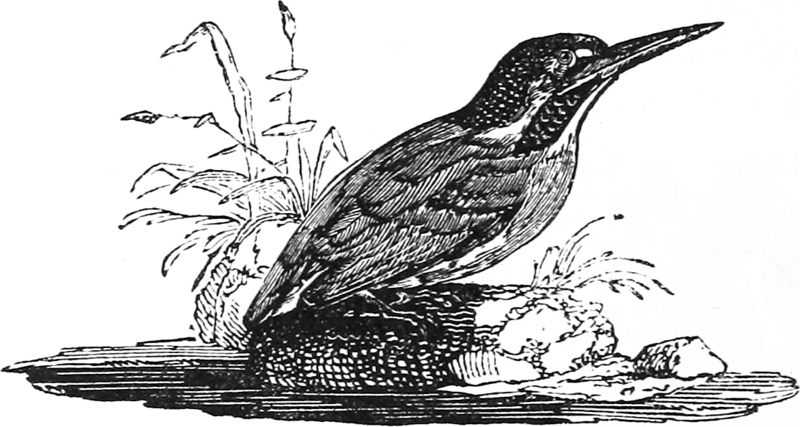
\includegraphics[scale=0.35]{images/Alycon.png}
        \end{figure}
        \vspace{0.5cm}
        \Huge
        \textbf{\textsc{Matematyka Dyskretna}}
        
        \vspace{0.5cm}
        \Large
        \textsc{Wybrane Dowody}
        
        \normalsize
        
        
        \line(1,0){330}
        
        \vspace{1cm}
        \textit{,,Myślę, że 7 punktów na 20 to nie jest zły wynik''}
        \vspace{1cm}

        \textit{\textsc{Popełnione przez}}\\
        \vspace{5mm}

        \textbf{\textsc{Dziurawy Ponton \\ Załatany Ponton \\ Puchaty Pompon \\ Zatopiony Ponton \\ Tonący Ponton \\ Notnop}}

        \vfill

        Kraków \\
        Anno Domini 2023
        
    \end{center}
    
\end{titlepage}


\tableofcontents
\section*{Licencja}
    \begin{figure}[h]
    	\begin{minipage}[c]{0.25\textwidth}
    		
\includegraphics[width=0.7\textwidth]{images/licencja.png}
    	\end{minipage}\hfill
    	\begin{minipage}[c]{0.75\textwidth}
    		\caption*{
    			Ten utwór jest dostępny na 
    			\href{https://creativecommons.org/licenses/by-sa/4.0/}{licencji Creative Commons Uznanie autorstwa
    			na tych samych warunkach 4.0 Międzynarodowe.}
    		}
    	\end{minipage}
    \end{figure}

% Actual content
\mainmatter

\chapter{Kombinatoryka}
 % Żeby nie było syfu to kolejne sekcje dodajemy do chapters/
% A potem includujemy za pomocą \input{chapters/...}

% Używamy \( \) i \[ \] zamiast dolarów -- tak jak się robi w LaTeXu


\documentclass[12pt, a4paper, polish, openany]{book}

% Please, let's familiarize ourselves with notatki.sty and tcs.sty so that we don't reinvent the wheel
\usepackage{notatki}

\fancyhead[L]{\textbf{\textit{MD}}}
\author{
}
\title{TCS and shitposting}


\begin{document}

% Front page and table of contents
\frontmatter

\input{titlepage}

\tableofcontents
\input{license}

% Actual content
\mainmatter

\chapter{Kombinatoryka}
\input{chapters/combinatorics/main}

\chapter{Zasada włączeń i wyłączeń}
\input{chapters/exclusion-inclusion/main}

\chapter{Posety}
\input{chapters/posets/main}

\chapter{Twierdzenie Ramseya}
\input{chapters/ramsey/main}

\chapter{Funkcje tworzące}
\input{chapters/generating_functions/main}

\chapter{Przepływy}
\input{chapters/flows/main}

\chapter{Skojarzenia}
\input{chapters/matchings/main}

\chapter{Kolorowanie grafów}
\input{chapters/graph-coloring/main}

\chapter{Grafy, ale nie kolorowanie}
\input{chapters/graph-misc/main}

\end{document}

\chapter{Zasada włączeń i wyłączeń}
 % Żeby nie było syfu to kolejne sekcje dodajemy do chapters/
% A potem includujemy za pomocą \input{chapters/...}

% Używamy \( \) i \[ \] zamiast dolarów -- tak jak się robi w LaTeXu


\documentclass[12pt, a4paper, polish, openany]{book}

% Please, let's familiarize ourselves with notatki.sty and tcs.sty so that we don't reinvent the wheel
\usepackage{notatki}

\fancyhead[L]{\textbf{\textit{MD}}}
\author{
}
\title{TCS and shitposting}


\begin{document}

% Front page and table of contents
\frontmatter

\input{titlepage}

\tableofcontents
\input{license}

% Actual content
\mainmatter

\chapter{Kombinatoryka}
\input{chapters/combinatorics/main}

\chapter{Zasada włączeń i wyłączeń}
\input{chapters/exclusion-inclusion/main}

\chapter{Posety}
\input{chapters/posets/main}

\chapter{Twierdzenie Ramseya}
\input{chapters/ramsey/main}

\chapter{Funkcje tworzące}
\input{chapters/generating_functions/main}

\chapter{Przepływy}
\input{chapters/flows/main}

\chapter{Skojarzenia}
\input{chapters/matchings/main}

\chapter{Kolorowanie grafów}
\input{chapters/graph-coloring/main}

\chapter{Grafy, ale nie kolorowanie}
\input{chapters/graph-misc/main}

\end{document}

\chapter{Posety}
 % Żeby nie było syfu to kolejne sekcje dodajemy do chapters/
% A potem includujemy za pomocą \input{chapters/...}

% Używamy \( \) i \[ \] zamiast dolarów -- tak jak się robi w LaTeXu


\documentclass[12pt, a4paper, polish, openany]{book}

% Please, let's familiarize ourselves with notatki.sty and tcs.sty so that we don't reinvent the wheel
\usepackage{notatki}

\fancyhead[L]{\textbf{\textit{MD}}}
\author{
}
\title{TCS and shitposting}


\begin{document}

% Front page and table of contents
\frontmatter

\input{titlepage}

\tableofcontents
\input{license}

% Actual content
\mainmatter

\chapter{Kombinatoryka}
\input{chapters/combinatorics/main}

\chapter{Zasada włączeń i wyłączeń}
\input{chapters/exclusion-inclusion/main}

\chapter{Posety}
\input{chapters/posets/main}

\chapter{Twierdzenie Ramseya}
\input{chapters/ramsey/main}

\chapter{Funkcje tworzące}
\input{chapters/generating_functions/main}

\chapter{Przepływy}
\input{chapters/flows/main}

\chapter{Skojarzenia}
\input{chapters/matchings/main}

\chapter{Kolorowanie grafów}
\input{chapters/graph-coloring/main}

\chapter{Grafy, ale nie kolorowanie}
\input{chapters/graph-misc/main}

\end{document}

\chapter{Twierdzenie Ramseya}
 % Żeby nie było syfu to kolejne sekcje dodajemy do chapters/
% A potem includujemy za pomocą \input{chapters/...}

% Używamy \( \) i \[ \] zamiast dolarów -- tak jak się robi w LaTeXu


\documentclass[12pt, a4paper, polish, openany]{book}

% Please, let's familiarize ourselves with notatki.sty and tcs.sty so that we don't reinvent the wheel
\usepackage{notatki}

\fancyhead[L]{\textbf{\textit{MD}}}
\author{
}
\title{TCS and shitposting}


\begin{document}

% Front page and table of contents
\frontmatter

\input{titlepage}

\tableofcontents
\input{license}

% Actual content
\mainmatter

\chapter{Kombinatoryka}
\input{chapters/combinatorics/main}

\chapter{Zasada włączeń i wyłączeń}
\input{chapters/exclusion-inclusion/main}

\chapter{Posety}
\input{chapters/posets/main}

\chapter{Twierdzenie Ramseya}
\input{chapters/ramsey/main}

\chapter{Funkcje tworzące}
\input{chapters/generating_functions/main}

\chapter{Przepływy}
\input{chapters/flows/main}

\chapter{Skojarzenia}
\input{chapters/matchings/main}

\chapter{Kolorowanie grafów}
\input{chapters/graph-coloring/main}

\chapter{Grafy, ale nie kolorowanie}
\input{chapters/graph-misc/main}

\end{document}

\chapter{Funkcje tworzące}
 % Żeby nie było syfu to kolejne sekcje dodajemy do chapters/
% A potem includujemy za pomocą \input{chapters/...}

% Używamy \( \) i \[ \] zamiast dolarów -- tak jak się robi w LaTeXu


\documentclass[12pt, a4paper, polish, openany]{book}

% Please, let's familiarize ourselves with notatki.sty and tcs.sty so that we don't reinvent the wheel
\usepackage{notatki}

\fancyhead[L]{\textbf{\textit{MD}}}
\author{
}
\title{TCS and shitposting}


\begin{document}

% Front page and table of contents
\frontmatter

\input{titlepage}

\tableofcontents
\input{license}

% Actual content
\mainmatter

\chapter{Kombinatoryka}
\input{chapters/combinatorics/main}

\chapter{Zasada włączeń i wyłączeń}
\input{chapters/exclusion-inclusion/main}

\chapter{Posety}
\input{chapters/posets/main}

\chapter{Twierdzenie Ramseya}
\input{chapters/ramsey/main}

\chapter{Funkcje tworzące}
\input{chapters/generating_functions/main}

\chapter{Przepływy}
\input{chapters/flows/main}

\chapter{Skojarzenia}
\input{chapters/matchings/main}

\chapter{Kolorowanie grafów}
\input{chapters/graph-coloring/main}

\chapter{Grafy, ale nie kolorowanie}
\input{chapters/graph-misc/main}

\end{document}

\chapter{Przepływy}
 % Żeby nie było syfu to kolejne sekcje dodajemy do chapters/
% A potem includujemy za pomocą \input{chapters/...}

% Używamy \( \) i \[ \] zamiast dolarów -- tak jak się robi w LaTeXu


\documentclass[12pt, a4paper, polish, openany]{book}

% Please, let's familiarize ourselves with notatki.sty and tcs.sty so that we don't reinvent the wheel
\usepackage{notatki}

\fancyhead[L]{\textbf{\textit{MD}}}
\author{
}
\title{TCS and shitposting}


\begin{document}

% Front page and table of contents
\frontmatter

\input{titlepage}

\tableofcontents
\input{license}

% Actual content
\mainmatter

\chapter{Kombinatoryka}
\input{chapters/combinatorics/main}

\chapter{Zasada włączeń i wyłączeń}
\input{chapters/exclusion-inclusion/main}

\chapter{Posety}
\input{chapters/posets/main}

\chapter{Twierdzenie Ramseya}
\input{chapters/ramsey/main}

\chapter{Funkcje tworzące}
\input{chapters/generating_functions/main}

\chapter{Przepływy}
\input{chapters/flows/main}

\chapter{Skojarzenia}
\input{chapters/matchings/main}

\chapter{Kolorowanie grafów}
\input{chapters/graph-coloring/main}

\chapter{Grafy, ale nie kolorowanie}
\input{chapters/graph-misc/main}

\end{document}

\chapter{Skojarzenia}
 % Żeby nie było syfu to kolejne sekcje dodajemy do chapters/
% A potem includujemy za pomocą \input{chapters/...}

% Używamy \( \) i \[ \] zamiast dolarów -- tak jak się robi w LaTeXu


\documentclass[12pt, a4paper, polish, openany]{book}

% Please, let's familiarize ourselves with notatki.sty and tcs.sty so that we don't reinvent the wheel
\usepackage{notatki}

\fancyhead[L]{\textbf{\textit{MD}}}
\author{
}
\title{TCS and shitposting}


\begin{document}

% Front page and table of contents
\frontmatter

\input{titlepage}

\tableofcontents
\input{license}

% Actual content
\mainmatter

\chapter{Kombinatoryka}
\input{chapters/combinatorics/main}

\chapter{Zasada włączeń i wyłączeń}
\input{chapters/exclusion-inclusion/main}

\chapter{Posety}
\input{chapters/posets/main}

\chapter{Twierdzenie Ramseya}
\input{chapters/ramsey/main}

\chapter{Funkcje tworzące}
\input{chapters/generating_functions/main}

\chapter{Przepływy}
\input{chapters/flows/main}

\chapter{Skojarzenia}
\input{chapters/matchings/main}

\chapter{Kolorowanie grafów}
\input{chapters/graph-coloring/main}

\chapter{Grafy, ale nie kolorowanie}
\input{chapters/graph-misc/main}

\end{document}

\chapter{Kolorowanie grafów}
 % Żeby nie było syfu to kolejne sekcje dodajemy do chapters/
% A potem includujemy za pomocą \input{chapters/...}

% Używamy \( \) i \[ \] zamiast dolarów -- tak jak się robi w LaTeXu


\documentclass[12pt, a4paper, polish, openany]{book}

% Please, let's familiarize ourselves with notatki.sty and tcs.sty so that we don't reinvent the wheel
\usepackage{notatki}

\fancyhead[L]{\textbf{\textit{MD}}}
\author{
}
\title{TCS and shitposting}


\begin{document}

% Front page and table of contents
\frontmatter

\input{titlepage}

\tableofcontents
\input{license}

% Actual content
\mainmatter

\chapter{Kombinatoryka}
\input{chapters/combinatorics/main}

\chapter{Zasada włączeń i wyłączeń}
\input{chapters/exclusion-inclusion/main}

\chapter{Posety}
\input{chapters/posets/main}

\chapter{Twierdzenie Ramseya}
\input{chapters/ramsey/main}

\chapter{Funkcje tworzące}
\input{chapters/generating_functions/main}

\chapter{Przepływy}
\input{chapters/flows/main}

\chapter{Skojarzenia}
\input{chapters/matchings/main}

\chapter{Kolorowanie grafów}
\input{chapters/graph-coloring/main}

\chapter{Grafy, ale nie kolorowanie}
\input{chapters/graph-misc/main}

\end{document}

\chapter{Grafy, ale nie kolorowanie}
 % Żeby nie było syfu to kolejne sekcje dodajemy do chapters/
% A potem includujemy za pomocą \input{chapters/...}

% Używamy \( \) i \[ \] zamiast dolarów -- tak jak się robi w LaTeXu


\documentclass[12pt, a4paper, polish, openany]{book}

% Please, let's familiarize ourselves with notatki.sty and tcs.sty so that we don't reinvent the wheel
\usepackage{notatki}

\fancyhead[L]{\textbf{\textit{MD}}}
\author{
}
\title{TCS and shitposting}


\begin{document}

% Front page and table of contents
\frontmatter

\input{titlepage}

\tableofcontents
\input{license}

% Actual content
\mainmatter

\chapter{Kombinatoryka}
\input{chapters/combinatorics/main}

\chapter{Zasada włączeń i wyłączeń}
\input{chapters/exclusion-inclusion/main}

\chapter{Posety}
\input{chapters/posets/main}

\chapter{Twierdzenie Ramseya}
\input{chapters/ramsey/main}

\chapter{Funkcje tworzące}
\input{chapters/generating_functions/main}

\chapter{Przepływy}
\input{chapters/flows/main}

\chapter{Skojarzenia}
\input{chapters/matchings/main}

\chapter{Kolorowanie grafów}
\input{chapters/graph-coloring/main}

\chapter{Grafy, ale nie kolorowanie}
\input{chapters/graph-misc/main}

\end{document}

\end{document}

\chapter{Grafy, ale nie kolorowanie}
 % Żeby nie było syfu to kolejne sekcje dodajemy do chapters/
% A potem includujemy za pomocą \input{chapters/...}

% Używamy \( \) i \[ \] zamiast dolarów -- tak jak się robi w LaTeXu


\documentclass[12pt, a4paper, polish, openany]{book}

% Please, let's familiarize ourselves with notatki.sty and tcs.sty so that we don't reinvent the wheel
\usepackage{notatki}

\fancyhead[L]{\textbf{\textit{MD}}}
\author{
}
\title{TCS and shitposting}


\begin{document}

% Front page and table of contents
\frontmatter

\begin{titlepage} 

    \begin{center}
         \begin{figure}[h]
            \centering
            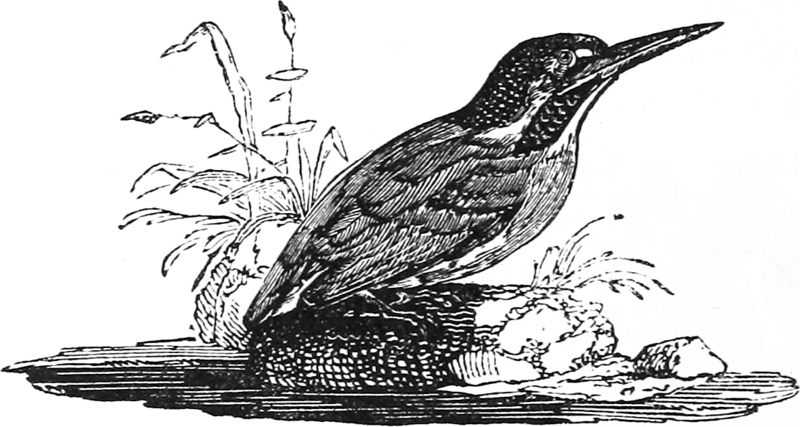
\includegraphics[scale=0.35]{images/Alycon.png}
        \end{figure}
        \vspace{0.5cm}
        \Huge
        \textbf{\textsc{Matematyka Dyskretna}}
        
        \vspace{0.5cm}
        \Large
        \textsc{Wybrane Dowody}
        
        \normalsize
        
        
        \line(1,0){330}
        
        \vspace{1cm}
        \textit{,,Myślę, że 7 punktów na 20 to nie jest zły wynik''}
        \vspace{1cm}

        \textit{\textsc{Popełnione przez}}\\
        \vspace{5mm}

        \textbf{\textsc{Dziurawy Ponton \\ Załatany Ponton \\ Puchaty Pompon \\ Zatopiony Ponton \\ Tonący Ponton \\ Notnop}}

        \vfill

        Kraków \\
        Anno Domini 2023
        
    \end{center}
    
\end{titlepage}


\tableofcontents
\section*{Licencja}
    \begin{figure}[h]
    	\begin{minipage}[c]{0.25\textwidth}
    		
\includegraphics[width=0.7\textwidth]{images/licencja.png}
    	\end{minipage}\hfill
    	\begin{minipage}[c]{0.75\textwidth}
    		\caption*{
    			Ten utwór jest dostępny na 
    			\href{https://creativecommons.org/licenses/by-sa/4.0/}{licencji Creative Commons Uznanie autorstwa
    			na tych samych warunkach 4.0 Międzynarodowe.}
    		}
    	\end{minipage}
    \end{figure}

% Actual content
\mainmatter

\chapter{Kombinatoryka}
 % Żeby nie było syfu to kolejne sekcje dodajemy do chapters/
% A potem includujemy za pomocą \input{chapters/...}

% Używamy \( \) i \[ \] zamiast dolarów -- tak jak się robi w LaTeXu


\documentclass[12pt, a4paper, polish, openany]{book}

% Please, let's familiarize ourselves with notatki.sty and tcs.sty so that we don't reinvent the wheel
\usepackage{notatki}

\fancyhead[L]{\textbf{\textit{MD}}}
\author{
}
\title{TCS and shitposting}


\begin{document}

% Front page and table of contents
\frontmatter

\input{titlepage}

\tableofcontents
\input{license}

% Actual content
\mainmatter

\chapter{Kombinatoryka}
\input{chapters/combinatorics/main}

\chapter{Zasada włączeń i wyłączeń}
\input{chapters/exclusion-inclusion/main}

\chapter{Posety}
\input{chapters/posets/main}

\chapter{Twierdzenie Ramseya}
\input{chapters/ramsey/main}

\chapter{Funkcje tworzące}
\input{chapters/generating_functions/main}

\chapter{Przepływy}
\input{chapters/flows/main}

\chapter{Skojarzenia}
\input{chapters/matchings/main}

\chapter{Kolorowanie grafów}
\input{chapters/graph-coloring/main}

\chapter{Grafy, ale nie kolorowanie}
\input{chapters/graph-misc/main}

\end{document}

\chapter{Zasada włączeń i wyłączeń}
 % Żeby nie było syfu to kolejne sekcje dodajemy do chapters/
% A potem includujemy za pomocą \input{chapters/...}

% Używamy \( \) i \[ \] zamiast dolarów -- tak jak się robi w LaTeXu


\documentclass[12pt, a4paper, polish, openany]{book}

% Please, let's familiarize ourselves with notatki.sty and tcs.sty so that we don't reinvent the wheel
\usepackage{notatki}

\fancyhead[L]{\textbf{\textit{MD}}}
\author{
}
\title{TCS and shitposting}


\begin{document}

% Front page and table of contents
\frontmatter

\input{titlepage}

\tableofcontents
\input{license}

% Actual content
\mainmatter

\chapter{Kombinatoryka}
\input{chapters/combinatorics/main}

\chapter{Zasada włączeń i wyłączeń}
\input{chapters/exclusion-inclusion/main}

\chapter{Posety}
\input{chapters/posets/main}

\chapter{Twierdzenie Ramseya}
\input{chapters/ramsey/main}

\chapter{Funkcje tworzące}
\input{chapters/generating_functions/main}

\chapter{Przepływy}
\input{chapters/flows/main}

\chapter{Skojarzenia}
\input{chapters/matchings/main}

\chapter{Kolorowanie grafów}
\input{chapters/graph-coloring/main}

\chapter{Grafy, ale nie kolorowanie}
\input{chapters/graph-misc/main}

\end{document}

\chapter{Posety}
 % Żeby nie było syfu to kolejne sekcje dodajemy do chapters/
% A potem includujemy za pomocą \input{chapters/...}

% Używamy \( \) i \[ \] zamiast dolarów -- tak jak się robi w LaTeXu


\documentclass[12pt, a4paper, polish, openany]{book}

% Please, let's familiarize ourselves with notatki.sty and tcs.sty so that we don't reinvent the wheel
\usepackage{notatki}

\fancyhead[L]{\textbf{\textit{MD}}}
\author{
}
\title{TCS and shitposting}


\begin{document}

% Front page and table of contents
\frontmatter

\input{titlepage}

\tableofcontents
\input{license}

% Actual content
\mainmatter

\chapter{Kombinatoryka}
\input{chapters/combinatorics/main}

\chapter{Zasada włączeń i wyłączeń}
\input{chapters/exclusion-inclusion/main}

\chapter{Posety}
\input{chapters/posets/main}

\chapter{Twierdzenie Ramseya}
\input{chapters/ramsey/main}

\chapter{Funkcje tworzące}
\input{chapters/generating_functions/main}

\chapter{Przepływy}
\input{chapters/flows/main}

\chapter{Skojarzenia}
\input{chapters/matchings/main}

\chapter{Kolorowanie grafów}
\input{chapters/graph-coloring/main}

\chapter{Grafy, ale nie kolorowanie}
\input{chapters/graph-misc/main}

\end{document}

\chapter{Twierdzenie Ramseya}
 % Żeby nie było syfu to kolejne sekcje dodajemy do chapters/
% A potem includujemy za pomocą \input{chapters/...}

% Używamy \( \) i \[ \] zamiast dolarów -- tak jak się robi w LaTeXu


\documentclass[12pt, a4paper, polish, openany]{book}

% Please, let's familiarize ourselves with notatki.sty and tcs.sty so that we don't reinvent the wheel
\usepackage{notatki}

\fancyhead[L]{\textbf{\textit{MD}}}
\author{
}
\title{TCS and shitposting}


\begin{document}

% Front page and table of contents
\frontmatter

\input{titlepage}

\tableofcontents
\input{license}

% Actual content
\mainmatter

\chapter{Kombinatoryka}
\input{chapters/combinatorics/main}

\chapter{Zasada włączeń i wyłączeń}
\input{chapters/exclusion-inclusion/main}

\chapter{Posety}
\input{chapters/posets/main}

\chapter{Twierdzenie Ramseya}
\input{chapters/ramsey/main}

\chapter{Funkcje tworzące}
\input{chapters/generating_functions/main}

\chapter{Przepływy}
\input{chapters/flows/main}

\chapter{Skojarzenia}
\input{chapters/matchings/main}

\chapter{Kolorowanie grafów}
\input{chapters/graph-coloring/main}

\chapter{Grafy, ale nie kolorowanie}
\input{chapters/graph-misc/main}

\end{document}

\chapter{Funkcje tworzące}
 % Żeby nie było syfu to kolejne sekcje dodajemy do chapters/
% A potem includujemy za pomocą \input{chapters/...}

% Używamy \( \) i \[ \] zamiast dolarów -- tak jak się robi w LaTeXu


\documentclass[12pt, a4paper, polish, openany]{book}

% Please, let's familiarize ourselves with notatki.sty and tcs.sty so that we don't reinvent the wheel
\usepackage{notatki}

\fancyhead[L]{\textbf{\textit{MD}}}
\author{
}
\title{TCS and shitposting}


\begin{document}

% Front page and table of contents
\frontmatter

\input{titlepage}

\tableofcontents
\input{license}

% Actual content
\mainmatter

\chapter{Kombinatoryka}
\input{chapters/combinatorics/main}

\chapter{Zasada włączeń i wyłączeń}
\input{chapters/exclusion-inclusion/main}

\chapter{Posety}
\input{chapters/posets/main}

\chapter{Twierdzenie Ramseya}
\input{chapters/ramsey/main}

\chapter{Funkcje tworzące}
\input{chapters/generating_functions/main}

\chapter{Przepływy}
\input{chapters/flows/main}

\chapter{Skojarzenia}
\input{chapters/matchings/main}

\chapter{Kolorowanie grafów}
\input{chapters/graph-coloring/main}

\chapter{Grafy, ale nie kolorowanie}
\input{chapters/graph-misc/main}

\end{document}

\chapter{Przepływy}
 % Żeby nie było syfu to kolejne sekcje dodajemy do chapters/
% A potem includujemy za pomocą \input{chapters/...}

% Używamy \( \) i \[ \] zamiast dolarów -- tak jak się robi w LaTeXu


\documentclass[12pt, a4paper, polish, openany]{book}

% Please, let's familiarize ourselves with notatki.sty and tcs.sty so that we don't reinvent the wheel
\usepackage{notatki}

\fancyhead[L]{\textbf{\textit{MD}}}
\author{
}
\title{TCS and shitposting}


\begin{document}

% Front page and table of contents
\frontmatter

\input{titlepage}

\tableofcontents
\input{license}

% Actual content
\mainmatter

\chapter{Kombinatoryka}
\input{chapters/combinatorics/main}

\chapter{Zasada włączeń i wyłączeń}
\input{chapters/exclusion-inclusion/main}

\chapter{Posety}
\input{chapters/posets/main}

\chapter{Twierdzenie Ramseya}
\input{chapters/ramsey/main}

\chapter{Funkcje tworzące}
\input{chapters/generating_functions/main}

\chapter{Przepływy}
\input{chapters/flows/main}

\chapter{Skojarzenia}
\input{chapters/matchings/main}

\chapter{Kolorowanie grafów}
\input{chapters/graph-coloring/main}

\chapter{Grafy, ale nie kolorowanie}
\input{chapters/graph-misc/main}

\end{document}

\chapter{Skojarzenia}
 % Żeby nie było syfu to kolejne sekcje dodajemy do chapters/
% A potem includujemy za pomocą \input{chapters/...}

% Używamy \( \) i \[ \] zamiast dolarów -- tak jak się robi w LaTeXu


\documentclass[12pt, a4paper, polish, openany]{book}

% Please, let's familiarize ourselves with notatki.sty and tcs.sty so that we don't reinvent the wheel
\usepackage{notatki}

\fancyhead[L]{\textbf{\textit{MD}}}
\author{
}
\title{TCS and shitposting}


\begin{document}

% Front page and table of contents
\frontmatter

\input{titlepage}

\tableofcontents
\input{license}

% Actual content
\mainmatter

\chapter{Kombinatoryka}
\input{chapters/combinatorics/main}

\chapter{Zasada włączeń i wyłączeń}
\input{chapters/exclusion-inclusion/main}

\chapter{Posety}
\input{chapters/posets/main}

\chapter{Twierdzenie Ramseya}
\input{chapters/ramsey/main}

\chapter{Funkcje tworzące}
\input{chapters/generating_functions/main}

\chapter{Przepływy}
\input{chapters/flows/main}

\chapter{Skojarzenia}
\input{chapters/matchings/main}

\chapter{Kolorowanie grafów}
\input{chapters/graph-coloring/main}

\chapter{Grafy, ale nie kolorowanie}
\input{chapters/graph-misc/main}

\end{document}

\chapter{Kolorowanie grafów}
 % Żeby nie było syfu to kolejne sekcje dodajemy do chapters/
% A potem includujemy za pomocą \input{chapters/...}

% Używamy \( \) i \[ \] zamiast dolarów -- tak jak się robi w LaTeXu


\documentclass[12pt, a4paper, polish, openany]{book}

% Please, let's familiarize ourselves with notatki.sty and tcs.sty so that we don't reinvent the wheel
\usepackage{notatki}

\fancyhead[L]{\textbf{\textit{MD}}}
\author{
}
\title{TCS and shitposting}


\begin{document}

% Front page and table of contents
\frontmatter

\input{titlepage}

\tableofcontents
\input{license}

% Actual content
\mainmatter

\chapter{Kombinatoryka}
\input{chapters/combinatorics/main}

\chapter{Zasada włączeń i wyłączeń}
\input{chapters/exclusion-inclusion/main}

\chapter{Posety}
\input{chapters/posets/main}

\chapter{Twierdzenie Ramseya}
\input{chapters/ramsey/main}

\chapter{Funkcje tworzące}
\input{chapters/generating_functions/main}

\chapter{Przepływy}
\input{chapters/flows/main}

\chapter{Skojarzenia}
\input{chapters/matchings/main}

\chapter{Kolorowanie grafów}
\input{chapters/graph-coloring/main}

\chapter{Grafy, ale nie kolorowanie}
\input{chapters/graph-misc/main}

\end{document}

\chapter{Grafy, ale nie kolorowanie}
 % Żeby nie było syfu to kolejne sekcje dodajemy do chapters/
% A potem includujemy za pomocą \input{chapters/...}

% Używamy \( \) i \[ \] zamiast dolarów -- tak jak się robi w LaTeXu


\documentclass[12pt, a4paper, polish, openany]{book}

% Please, let's familiarize ourselves with notatki.sty and tcs.sty so that we don't reinvent the wheel
\usepackage{notatki}

\fancyhead[L]{\textbf{\textit{MD}}}
\author{
}
\title{TCS and shitposting}


\begin{document}

% Front page and table of contents
\frontmatter

\input{titlepage}

\tableofcontents
\input{license}

% Actual content
\mainmatter

\chapter{Kombinatoryka}
\input{chapters/combinatorics/main}

\chapter{Zasada włączeń i wyłączeń}
\input{chapters/exclusion-inclusion/main}

\chapter{Posety}
\input{chapters/posets/main}

\chapter{Twierdzenie Ramseya}
\input{chapters/ramsey/main}

\chapter{Funkcje tworzące}
\input{chapters/generating_functions/main}

\chapter{Przepływy}
\input{chapters/flows/main}

\chapter{Skojarzenia}
\input{chapters/matchings/main}

\chapter{Kolorowanie grafów}
\input{chapters/graph-coloring/main}

\chapter{Grafy, ale nie kolorowanie}
\input{chapters/graph-misc/main}

\end{document}

\end{document}

\end{document}

\section{Omów zamkniętość klasy języków regularnych na operacje na językach}
 % Żeby nie było syfu to kolejne sekcje dodajemy do chapters/
% A potem includujemy za pomocą \input{chapters/...}

% Używamy \( \) i \[ \] zamiast dolarów -- tak jak się robi w LaTeXu


\documentclass[12pt, a4paper, polish, openany]{book}

% Please, let's familiarize ourselves with notatki.sty and tcs.sty so that we don't reinvent the wheel
\usepackage{notatki}

\fancyhead[L]{\textbf{\textit{MD}}}
\author{
}
\title{TCS and shitposting}


\begin{document}

% Front page and table of contents
\frontmatter

\begin{titlepage} 

    \begin{center}
         \begin{figure}[h]
            \centering
            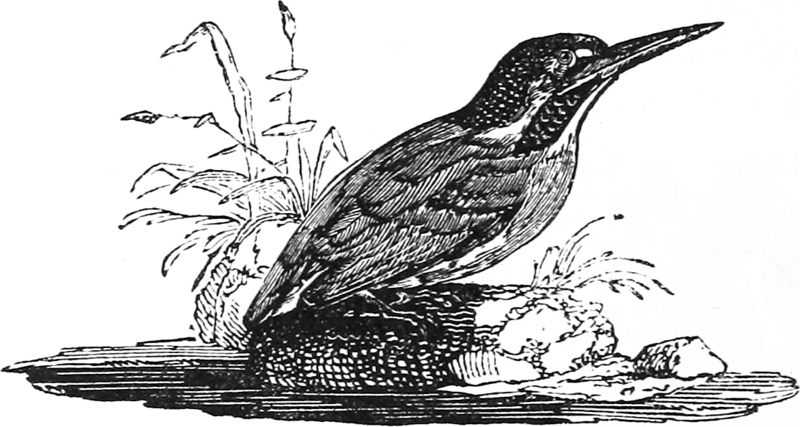
\includegraphics[scale=0.35]{images/Alycon.png}
        \end{figure}
        \vspace{0.5cm}
        \Huge
        \textbf{\textsc{Matematyka Dyskretna}}
        
        \vspace{0.5cm}
        \Large
        \textsc{Wybrane Dowody}
        
        \normalsize
        
        
        \line(1,0){330}
        
        \vspace{1cm}
        \textit{,,Myślę, że 7 punktów na 20 to nie jest zły wynik''}
        \vspace{1cm}

        \textit{\textsc{Popełnione przez}}\\
        \vspace{5mm}

        \textbf{\textsc{Dziurawy Ponton \\ Załatany Ponton \\ Puchaty Pompon \\ Zatopiony Ponton \\ Tonący Ponton \\ Notnop}}

        \vfill

        Kraków \\
        Anno Domini 2023
        
    \end{center}
    
\end{titlepage}


\tableofcontents
\section*{Licencja}
    \begin{figure}[h]
    	\begin{minipage}[c]{0.25\textwidth}
    		
\includegraphics[width=0.7\textwidth]{images/licencja.png}
    	\end{minipage}\hfill
    	\begin{minipage}[c]{0.75\textwidth}
    		\caption*{
    			Ten utwór jest dostępny na 
    			\href{https://creativecommons.org/licenses/by-sa/4.0/}{licencji Creative Commons Uznanie autorstwa
    			na tych samych warunkach 4.0 Międzynarodowe.}
    		}
    	\end{minipage}
    \end{figure}

% Actual content
\mainmatter

\chapter{Kombinatoryka}
 % Żeby nie było syfu to kolejne sekcje dodajemy do chapters/
% A potem includujemy za pomocą \input{chapters/...}

% Używamy \( \) i \[ \] zamiast dolarów -- tak jak się robi w LaTeXu


\documentclass[12pt, a4paper, polish, openany]{book}

% Please, let's familiarize ourselves with notatki.sty and tcs.sty so that we don't reinvent the wheel
\usepackage{notatki}

\fancyhead[L]{\textbf{\textit{MD}}}
\author{
}
\title{TCS and shitposting}


\begin{document}

% Front page and table of contents
\frontmatter

\begin{titlepage} 

    \begin{center}
         \begin{figure}[h]
            \centering
            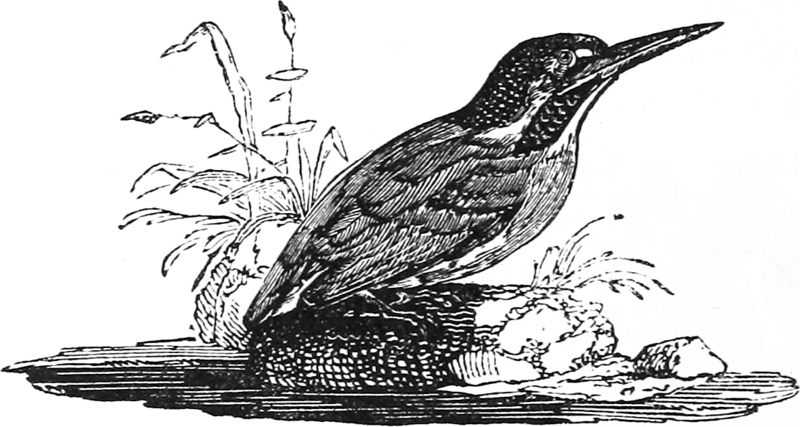
\includegraphics[scale=0.35]{images/Alycon.png}
        \end{figure}
        \vspace{0.5cm}
        \Huge
        \textbf{\textsc{Matematyka Dyskretna}}
        
        \vspace{0.5cm}
        \Large
        \textsc{Wybrane Dowody}
        
        \normalsize
        
        
        \line(1,0){330}
        
        \vspace{1cm}
        \textit{,,Myślę, że 7 punktów na 20 to nie jest zły wynik''}
        \vspace{1cm}

        \textit{\textsc{Popełnione przez}}\\
        \vspace{5mm}

        \textbf{\textsc{Dziurawy Ponton \\ Załatany Ponton \\ Puchaty Pompon \\ Zatopiony Ponton \\ Tonący Ponton \\ Notnop}}

        \vfill

        Kraków \\
        Anno Domini 2023
        
    \end{center}
    
\end{titlepage}


\tableofcontents
\section*{Licencja}
    \begin{figure}[h]
    	\begin{minipage}[c]{0.25\textwidth}
    		
\includegraphics[width=0.7\textwidth]{images/licencja.png}
    	\end{minipage}\hfill
    	\begin{minipage}[c]{0.75\textwidth}
    		\caption*{
    			Ten utwór jest dostępny na 
    			\href{https://creativecommons.org/licenses/by-sa/4.0/}{licencji Creative Commons Uznanie autorstwa
    			na tych samych warunkach 4.0 Międzynarodowe.}
    		}
    	\end{minipage}
    \end{figure}

% Actual content
\mainmatter

\chapter{Kombinatoryka}
 % Żeby nie było syfu to kolejne sekcje dodajemy do chapters/
% A potem includujemy za pomocą \input{chapters/...}

% Używamy \( \) i \[ \] zamiast dolarów -- tak jak się robi w LaTeXu


\documentclass[12pt, a4paper, polish, openany]{book}

% Please, let's familiarize ourselves with notatki.sty and tcs.sty so that we don't reinvent the wheel
\usepackage{notatki}

\fancyhead[L]{\textbf{\textit{MD}}}
\author{
}
\title{TCS and shitposting}


\begin{document}

% Front page and table of contents
\frontmatter

\input{titlepage}

\tableofcontents
\input{license}

% Actual content
\mainmatter

\chapter{Kombinatoryka}
\input{chapters/combinatorics/main}

\chapter{Zasada włączeń i wyłączeń}
\input{chapters/exclusion-inclusion/main}

\chapter{Posety}
\input{chapters/posets/main}

\chapter{Twierdzenie Ramseya}
\input{chapters/ramsey/main}

\chapter{Funkcje tworzące}
\input{chapters/generating_functions/main}

\chapter{Przepływy}
\input{chapters/flows/main}

\chapter{Skojarzenia}
\input{chapters/matchings/main}

\chapter{Kolorowanie grafów}
\input{chapters/graph-coloring/main}

\chapter{Grafy, ale nie kolorowanie}
\input{chapters/graph-misc/main}

\end{document}

\chapter{Zasada włączeń i wyłączeń}
 % Żeby nie było syfu to kolejne sekcje dodajemy do chapters/
% A potem includujemy za pomocą \input{chapters/...}

% Używamy \( \) i \[ \] zamiast dolarów -- tak jak się robi w LaTeXu


\documentclass[12pt, a4paper, polish, openany]{book}

% Please, let's familiarize ourselves with notatki.sty and tcs.sty so that we don't reinvent the wheel
\usepackage{notatki}

\fancyhead[L]{\textbf{\textit{MD}}}
\author{
}
\title{TCS and shitposting}


\begin{document}

% Front page and table of contents
\frontmatter

\input{titlepage}

\tableofcontents
\input{license}

% Actual content
\mainmatter

\chapter{Kombinatoryka}
\input{chapters/combinatorics/main}

\chapter{Zasada włączeń i wyłączeń}
\input{chapters/exclusion-inclusion/main}

\chapter{Posety}
\input{chapters/posets/main}

\chapter{Twierdzenie Ramseya}
\input{chapters/ramsey/main}

\chapter{Funkcje tworzące}
\input{chapters/generating_functions/main}

\chapter{Przepływy}
\input{chapters/flows/main}

\chapter{Skojarzenia}
\input{chapters/matchings/main}

\chapter{Kolorowanie grafów}
\input{chapters/graph-coloring/main}

\chapter{Grafy, ale nie kolorowanie}
\input{chapters/graph-misc/main}

\end{document}

\chapter{Posety}
 % Żeby nie było syfu to kolejne sekcje dodajemy do chapters/
% A potem includujemy za pomocą \input{chapters/...}

% Używamy \( \) i \[ \] zamiast dolarów -- tak jak się robi w LaTeXu


\documentclass[12pt, a4paper, polish, openany]{book}

% Please, let's familiarize ourselves with notatki.sty and tcs.sty so that we don't reinvent the wheel
\usepackage{notatki}

\fancyhead[L]{\textbf{\textit{MD}}}
\author{
}
\title{TCS and shitposting}


\begin{document}

% Front page and table of contents
\frontmatter

\input{titlepage}

\tableofcontents
\input{license}

% Actual content
\mainmatter

\chapter{Kombinatoryka}
\input{chapters/combinatorics/main}

\chapter{Zasada włączeń i wyłączeń}
\input{chapters/exclusion-inclusion/main}

\chapter{Posety}
\input{chapters/posets/main}

\chapter{Twierdzenie Ramseya}
\input{chapters/ramsey/main}

\chapter{Funkcje tworzące}
\input{chapters/generating_functions/main}

\chapter{Przepływy}
\input{chapters/flows/main}

\chapter{Skojarzenia}
\input{chapters/matchings/main}

\chapter{Kolorowanie grafów}
\input{chapters/graph-coloring/main}

\chapter{Grafy, ale nie kolorowanie}
\input{chapters/graph-misc/main}

\end{document}

\chapter{Twierdzenie Ramseya}
 % Żeby nie było syfu to kolejne sekcje dodajemy do chapters/
% A potem includujemy za pomocą \input{chapters/...}

% Używamy \( \) i \[ \] zamiast dolarów -- tak jak się robi w LaTeXu


\documentclass[12pt, a4paper, polish, openany]{book}

% Please, let's familiarize ourselves with notatki.sty and tcs.sty so that we don't reinvent the wheel
\usepackage{notatki}

\fancyhead[L]{\textbf{\textit{MD}}}
\author{
}
\title{TCS and shitposting}


\begin{document}

% Front page and table of contents
\frontmatter

\input{titlepage}

\tableofcontents
\input{license}

% Actual content
\mainmatter

\chapter{Kombinatoryka}
\input{chapters/combinatorics/main}

\chapter{Zasada włączeń i wyłączeń}
\input{chapters/exclusion-inclusion/main}

\chapter{Posety}
\input{chapters/posets/main}

\chapter{Twierdzenie Ramseya}
\input{chapters/ramsey/main}

\chapter{Funkcje tworzące}
\input{chapters/generating_functions/main}

\chapter{Przepływy}
\input{chapters/flows/main}

\chapter{Skojarzenia}
\input{chapters/matchings/main}

\chapter{Kolorowanie grafów}
\input{chapters/graph-coloring/main}

\chapter{Grafy, ale nie kolorowanie}
\input{chapters/graph-misc/main}

\end{document}

\chapter{Funkcje tworzące}
 % Żeby nie było syfu to kolejne sekcje dodajemy do chapters/
% A potem includujemy za pomocą \input{chapters/...}

% Używamy \( \) i \[ \] zamiast dolarów -- tak jak się robi w LaTeXu


\documentclass[12pt, a4paper, polish, openany]{book}

% Please, let's familiarize ourselves with notatki.sty and tcs.sty so that we don't reinvent the wheel
\usepackage{notatki}

\fancyhead[L]{\textbf{\textit{MD}}}
\author{
}
\title{TCS and shitposting}


\begin{document}

% Front page and table of contents
\frontmatter

\input{titlepage}

\tableofcontents
\input{license}

% Actual content
\mainmatter

\chapter{Kombinatoryka}
\input{chapters/combinatorics/main}

\chapter{Zasada włączeń i wyłączeń}
\input{chapters/exclusion-inclusion/main}

\chapter{Posety}
\input{chapters/posets/main}

\chapter{Twierdzenie Ramseya}
\input{chapters/ramsey/main}

\chapter{Funkcje tworzące}
\input{chapters/generating_functions/main}

\chapter{Przepływy}
\input{chapters/flows/main}

\chapter{Skojarzenia}
\input{chapters/matchings/main}

\chapter{Kolorowanie grafów}
\input{chapters/graph-coloring/main}

\chapter{Grafy, ale nie kolorowanie}
\input{chapters/graph-misc/main}

\end{document}

\chapter{Przepływy}
 % Żeby nie było syfu to kolejne sekcje dodajemy do chapters/
% A potem includujemy za pomocą \input{chapters/...}

% Używamy \( \) i \[ \] zamiast dolarów -- tak jak się robi w LaTeXu


\documentclass[12pt, a4paper, polish, openany]{book}

% Please, let's familiarize ourselves with notatki.sty and tcs.sty so that we don't reinvent the wheel
\usepackage{notatki}

\fancyhead[L]{\textbf{\textit{MD}}}
\author{
}
\title{TCS and shitposting}


\begin{document}

% Front page and table of contents
\frontmatter

\input{titlepage}

\tableofcontents
\input{license}

% Actual content
\mainmatter

\chapter{Kombinatoryka}
\input{chapters/combinatorics/main}

\chapter{Zasada włączeń i wyłączeń}
\input{chapters/exclusion-inclusion/main}

\chapter{Posety}
\input{chapters/posets/main}

\chapter{Twierdzenie Ramseya}
\input{chapters/ramsey/main}

\chapter{Funkcje tworzące}
\input{chapters/generating_functions/main}

\chapter{Przepływy}
\input{chapters/flows/main}

\chapter{Skojarzenia}
\input{chapters/matchings/main}

\chapter{Kolorowanie grafów}
\input{chapters/graph-coloring/main}

\chapter{Grafy, ale nie kolorowanie}
\input{chapters/graph-misc/main}

\end{document}

\chapter{Skojarzenia}
 % Żeby nie było syfu to kolejne sekcje dodajemy do chapters/
% A potem includujemy za pomocą \input{chapters/...}

% Używamy \( \) i \[ \] zamiast dolarów -- tak jak się robi w LaTeXu


\documentclass[12pt, a4paper, polish, openany]{book}

% Please, let's familiarize ourselves with notatki.sty and tcs.sty so that we don't reinvent the wheel
\usepackage{notatki}

\fancyhead[L]{\textbf{\textit{MD}}}
\author{
}
\title{TCS and shitposting}


\begin{document}

% Front page and table of contents
\frontmatter

\input{titlepage}

\tableofcontents
\input{license}

% Actual content
\mainmatter

\chapter{Kombinatoryka}
\input{chapters/combinatorics/main}

\chapter{Zasada włączeń i wyłączeń}
\input{chapters/exclusion-inclusion/main}

\chapter{Posety}
\input{chapters/posets/main}

\chapter{Twierdzenie Ramseya}
\input{chapters/ramsey/main}

\chapter{Funkcje tworzące}
\input{chapters/generating_functions/main}

\chapter{Przepływy}
\input{chapters/flows/main}

\chapter{Skojarzenia}
\input{chapters/matchings/main}

\chapter{Kolorowanie grafów}
\input{chapters/graph-coloring/main}

\chapter{Grafy, ale nie kolorowanie}
\input{chapters/graph-misc/main}

\end{document}

\chapter{Kolorowanie grafów}
 % Żeby nie było syfu to kolejne sekcje dodajemy do chapters/
% A potem includujemy za pomocą \input{chapters/...}

% Używamy \( \) i \[ \] zamiast dolarów -- tak jak się robi w LaTeXu


\documentclass[12pt, a4paper, polish, openany]{book}

% Please, let's familiarize ourselves with notatki.sty and tcs.sty so that we don't reinvent the wheel
\usepackage{notatki}

\fancyhead[L]{\textbf{\textit{MD}}}
\author{
}
\title{TCS and shitposting}


\begin{document}

% Front page and table of contents
\frontmatter

\input{titlepage}

\tableofcontents
\input{license}

% Actual content
\mainmatter

\chapter{Kombinatoryka}
\input{chapters/combinatorics/main}

\chapter{Zasada włączeń i wyłączeń}
\input{chapters/exclusion-inclusion/main}

\chapter{Posety}
\input{chapters/posets/main}

\chapter{Twierdzenie Ramseya}
\input{chapters/ramsey/main}

\chapter{Funkcje tworzące}
\input{chapters/generating_functions/main}

\chapter{Przepływy}
\input{chapters/flows/main}

\chapter{Skojarzenia}
\input{chapters/matchings/main}

\chapter{Kolorowanie grafów}
\input{chapters/graph-coloring/main}

\chapter{Grafy, ale nie kolorowanie}
\input{chapters/graph-misc/main}

\end{document}

\chapter{Grafy, ale nie kolorowanie}
 % Żeby nie było syfu to kolejne sekcje dodajemy do chapters/
% A potem includujemy za pomocą \input{chapters/...}

% Używamy \( \) i \[ \] zamiast dolarów -- tak jak się robi w LaTeXu


\documentclass[12pt, a4paper, polish, openany]{book}

% Please, let's familiarize ourselves with notatki.sty and tcs.sty so that we don't reinvent the wheel
\usepackage{notatki}

\fancyhead[L]{\textbf{\textit{MD}}}
\author{
}
\title{TCS and shitposting}


\begin{document}

% Front page and table of contents
\frontmatter

\input{titlepage}

\tableofcontents
\input{license}

% Actual content
\mainmatter

\chapter{Kombinatoryka}
\input{chapters/combinatorics/main}

\chapter{Zasada włączeń i wyłączeń}
\input{chapters/exclusion-inclusion/main}

\chapter{Posety}
\input{chapters/posets/main}

\chapter{Twierdzenie Ramseya}
\input{chapters/ramsey/main}

\chapter{Funkcje tworzące}
\input{chapters/generating_functions/main}

\chapter{Przepływy}
\input{chapters/flows/main}

\chapter{Skojarzenia}
\input{chapters/matchings/main}

\chapter{Kolorowanie grafów}
\input{chapters/graph-coloring/main}

\chapter{Grafy, ale nie kolorowanie}
\input{chapters/graph-misc/main}

\end{document}

\end{document}

\chapter{Zasada włączeń i wyłączeń}
 % Żeby nie było syfu to kolejne sekcje dodajemy do chapters/
% A potem includujemy za pomocą \input{chapters/...}

% Używamy \( \) i \[ \] zamiast dolarów -- tak jak się robi w LaTeXu


\documentclass[12pt, a4paper, polish, openany]{book}

% Please, let's familiarize ourselves with notatki.sty and tcs.sty so that we don't reinvent the wheel
\usepackage{notatki}

\fancyhead[L]{\textbf{\textit{MD}}}
\author{
}
\title{TCS and shitposting}


\begin{document}

% Front page and table of contents
\frontmatter

\begin{titlepage} 

    \begin{center}
         \begin{figure}[h]
            \centering
            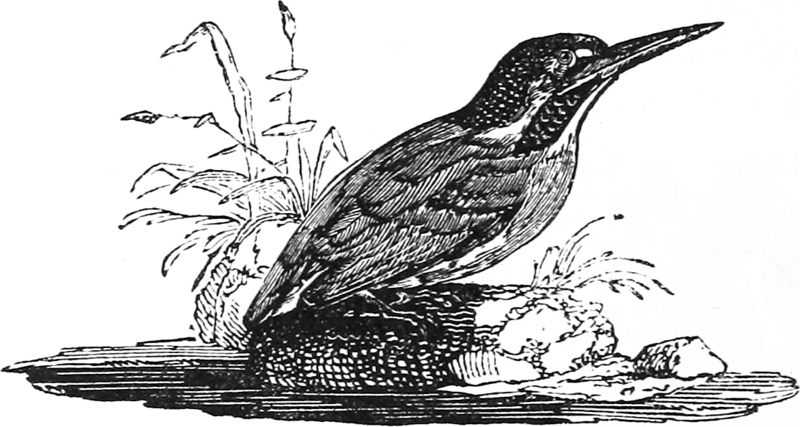
\includegraphics[scale=0.35]{images/Alycon.png}
        \end{figure}
        \vspace{0.5cm}
        \Huge
        \textbf{\textsc{Matematyka Dyskretna}}
        
        \vspace{0.5cm}
        \Large
        \textsc{Wybrane Dowody}
        
        \normalsize
        
        
        \line(1,0){330}
        
        \vspace{1cm}
        \textit{,,Myślę, że 7 punktów na 20 to nie jest zły wynik''}
        \vspace{1cm}

        \textit{\textsc{Popełnione przez}}\\
        \vspace{5mm}

        \textbf{\textsc{Dziurawy Ponton \\ Załatany Ponton \\ Puchaty Pompon \\ Zatopiony Ponton \\ Tonący Ponton \\ Notnop}}

        \vfill

        Kraków \\
        Anno Domini 2023
        
    \end{center}
    
\end{titlepage}


\tableofcontents
\section*{Licencja}
    \begin{figure}[h]
    	\begin{minipage}[c]{0.25\textwidth}
    		
\includegraphics[width=0.7\textwidth]{images/licencja.png}
    	\end{minipage}\hfill
    	\begin{minipage}[c]{0.75\textwidth}
    		\caption*{
    			Ten utwór jest dostępny na 
    			\href{https://creativecommons.org/licenses/by-sa/4.0/}{licencji Creative Commons Uznanie autorstwa
    			na tych samych warunkach 4.0 Międzynarodowe.}
    		}
    	\end{minipage}
    \end{figure}

% Actual content
\mainmatter

\chapter{Kombinatoryka}
 % Żeby nie było syfu to kolejne sekcje dodajemy do chapters/
% A potem includujemy za pomocą \input{chapters/...}

% Używamy \( \) i \[ \] zamiast dolarów -- tak jak się robi w LaTeXu


\documentclass[12pt, a4paper, polish, openany]{book}

% Please, let's familiarize ourselves with notatki.sty and tcs.sty so that we don't reinvent the wheel
\usepackage{notatki}

\fancyhead[L]{\textbf{\textit{MD}}}
\author{
}
\title{TCS and shitposting}


\begin{document}

% Front page and table of contents
\frontmatter

\input{titlepage}

\tableofcontents
\input{license}

% Actual content
\mainmatter

\chapter{Kombinatoryka}
\input{chapters/combinatorics/main}

\chapter{Zasada włączeń i wyłączeń}
\input{chapters/exclusion-inclusion/main}

\chapter{Posety}
\input{chapters/posets/main}

\chapter{Twierdzenie Ramseya}
\input{chapters/ramsey/main}

\chapter{Funkcje tworzące}
\input{chapters/generating_functions/main}

\chapter{Przepływy}
\input{chapters/flows/main}

\chapter{Skojarzenia}
\input{chapters/matchings/main}

\chapter{Kolorowanie grafów}
\input{chapters/graph-coloring/main}

\chapter{Grafy, ale nie kolorowanie}
\input{chapters/graph-misc/main}

\end{document}

\chapter{Zasada włączeń i wyłączeń}
 % Żeby nie było syfu to kolejne sekcje dodajemy do chapters/
% A potem includujemy za pomocą \input{chapters/...}

% Używamy \( \) i \[ \] zamiast dolarów -- tak jak się robi w LaTeXu


\documentclass[12pt, a4paper, polish, openany]{book}

% Please, let's familiarize ourselves with notatki.sty and tcs.sty so that we don't reinvent the wheel
\usepackage{notatki}

\fancyhead[L]{\textbf{\textit{MD}}}
\author{
}
\title{TCS and shitposting}


\begin{document}

% Front page and table of contents
\frontmatter

\input{titlepage}

\tableofcontents
\input{license}

% Actual content
\mainmatter

\chapter{Kombinatoryka}
\input{chapters/combinatorics/main}

\chapter{Zasada włączeń i wyłączeń}
\input{chapters/exclusion-inclusion/main}

\chapter{Posety}
\input{chapters/posets/main}

\chapter{Twierdzenie Ramseya}
\input{chapters/ramsey/main}

\chapter{Funkcje tworzące}
\input{chapters/generating_functions/main}

\chapter{Przepływy}
\input{chapters/flows/main}

\chapter{Skojarzenia}
\input{chapters/matchings/main}

\chapter{Kolorowanie grafów}
\input{chapters/graph-coloring/main}

\chapter{Grafy, ale nie kolorowanie}
\input{chapters/graph-misc/main}

\end{document}

\chapter{Posety}
 % Żeby nie było syfu to kolejne sekcje dodajemy do chapters/
% A potem includujemy za pomocą \input{chapters/...}

% Używamy \( \) i \[ \] zamiast dolarów -- tak jak się robi w LaTeXu


\documentclass[12pt, a4paper, polish, openany]{book}

% Please, let's familiarize ourselves with notatki.sty and tcs.sty so that we don't reinvent the wheel
\usepackage{notatki}

\fancyhead[L]{\textbf{\textit{MD}}}
\author{
}
\title{TCS and shitposting}


\begin{document}

% Front page and table of contents
\frontmatter

\input{titlepage}

\tableofcontents
\input{license}

% Actual content
\mainmatter

\chapter{Kombinatoryka}
\input{chapters/combinatorics/main}

\chapter{Zasada włączeń i wyłączeń}
\input{chapters/exclusion-inclusion/main}

\chapter{Posety}
\input{chapters/posets/main}

\chapter{Twierdzenie Ramseya}
\input{chapters/ramsey/main}

\chapter{Funkcje tworzące}
\input{chapters/generating_functions/main}

\chapter{Przepływy}
\input{chapters/flows/main}

\chapter{Skojarzenia}
\input{chapters/matchings/main}

\chapter{Kolorowanie grafów}
\input{chapters/graph-coloring/main}

\chapter{Grafy, ale nie kolorowanie}
\input{chapters/graph-misc/main}

\end{document}

\chapter{Twierdzenie Ramseya}
 % Żeby nie było syfu to kolejne sekcje dodajemy do chapters/
% A potem includujemy za pomocą \input{chapters/...}

% Używamy \( \) i \[ \] zamiast dolarów -- tak jak się robi w LaTeXu


\documentclass[12pt, a4paper, polish, openany]{book}

% Please, let's familiarize ourselves with notatki.sty and tcs.sty so that we don't reinvent the wheel
\usepackage{notatki}

\fancyhead[L]{\textbf{\textit{MD}}}
\author{
}
\title{TCS and shitposting}


\begin{document}

% Front page and table of contents
\frontmatter

\input{titlepage}

\tableofcontents
\input{license}

% Actual content
\mainmatter

\chapter{Kombinatoryka}
\input{chapters/combinatorics/main}

\chapter{Zasada włączeń i wyłączeń}
\input{chapters/exclusion-inclusion/main}

\chapter{Posety}
\input{chapters/posets/main}

\chapter{Twierdzenie Ramseya}
\input{chapters/ramsey/main}

\chapter{Funkcje tworzące}
\input{chapters/generating_functions/main}

\chapter{Przepływy}
\input{chapters/flows/main}

\chapter{Skojarzenia}
\input{chapters/matchings/main}

\chapter{Kolorowanie grafów}
\input{chapters/graph-coloring/main}

\chapter{Grafy, ale nie kolorowanie}
\input{chapters/graph-misc/main}

\end{document}

\chapter{Funkcje tworzące}
 % Żeby nie było syfu to kolejne sekcje dodajemy do chapters/
% A potem includujemy za pomocą \input{chapters/...}

% Używamy \( \) i \[ \] zamiast dolarów -- tak jak się robi w LaTeXu


\documentclass[12pt, a4paper, polish, openany]{book}

% Please, let's familiarize ourselves with notatki.sty and tcs.sty so that we don't reinvent the wheel
\usepackage{notatki}

\fancyhead[L]{\textbf{\textit{MD}}}
\author{
}
\title{TCS and shitposting}


\begin{document}

% Front page and table of contents
\frontmatter

\input{titlepage}

\tableofcontents
\input{license}

% Actual content
\mainmatter

\chapter{Kombinatoryka}
\input{chapters/combinatorics/main}

\chapter{Zasada włączeń i wyłączeń}
\input{chapters/exclusion-inclusion/main}

\chapter{Posety}
\input{chapters/posets/main}

\chapter{Twierdzenie Ramseya}
\input{chapters/ramsey/main}

\chapter{Funkcje tworzące}
\input{chapters/generating_functions/main}

\chapter{Przepływy}
\input{chapters/flows/main}

\chapter{Skojarzenia}
\input{chapters/matchings/main}

\chapter{Kolorowanie grafów}
\input{chapters/graph-coloring/main}

\chapter{Grafy, ale nie kolorowanie}
\input{chapters/graph-misc/main}

\end{document}

\chapter{Przepływy}
 % Żeby nie było syfu to kolejne sekcje dodajemy do chapters/
% A potem includujemy za pomocą \input{chapters/...}

% Używamy \( \) i \[ \] zamiast dolarów -- tak jak się robi w LaTeXu


\documentclass[12pt, a4paper, polish, openany]{book}

% Please, let's familiarize ourselves with notatki.sty and tcs.sty so that we don't reinvent the wheel
\usepackage{notatki}

\fancyhead[L]{\textbf{\textit{MD}}}
\author{
}
\title{TCS and shitposting}


\begin{document}

% Front page and table of contents
\frontmatter

\input{titlepage}

\tableofcontents
\input{license}

% Actual content
\mainmatter

\chapter{Kombinatoryka}
\input{chapters/combinatorics/main}

\chapter{Zasada włączeń i wyłączeń}
\input{chapters/exclusion-inclusion/main}

\chapter{Posety}
\input{chapters/posets/main}

\chapter{Twierdzenie Ramseya}
\input{chapters/ramsey/main}

\chapter{Funkcje tworzące}
\input{chapters/generating_functions/main}

\chapter{Przepływy}
\input{chapters/flows/main}

\chapter{Skojarzenia}
\input{chapters/matchings/main}

\chapter{Kolorowanie grafów}
\input{chapters/graph-coloring/main}

\chapter{Grafy, ale nie kolorowanie}
\input{chapters/graph-misc/main}

\end{document}

\chapter{Skojarzenia}
 % Żeby nie było syfu to kolejne sekcje dodajemy do chapters/
% A potem includujemy za pomocą \input{chapters/...}

% Używamy \( \) i \[ \] zamiast dolarów -- tak jak się robi w LaTeXu


\documentclass[12pt, a4paper, polish, openany]{book}

% Please, let's familiarize ourselves with notatki.sty and tcs.sty so that we don't reinvent the wheel
\usepackage{notatki}

\fancyhead[L]{\textbf{\textit{MD}}}
\author{
}
\title{TCS and shitposting}


\begin{document}

% Front page and table of contents
\frontmatter

\input{titlepage}

\tableofcontents
\input{license}

% Actual content
\mainmatter

\chapter{Kombinatoryka}
\input{chapters/combinatorics/main}

\chapter{Zasada włączeń i wyłączeń}
\input{chapters/exclusion-inclusion/main}

\chapter{Posety}
\input{chapters/posets/main}

\chapter{Twierdzenie Ramseya}
\input{chapters/ramsey/main}

\chapter{Funkcje tworzące}
\input{chapters/generating_functions/main}

\chapter{Przepływy}
\input{chapters/flows/main}

\chapter{Skojarzenia}
\input{chapters/matchings/main}

\chapter{Kolorowanie grafów}
\input{chapters/graph-coloring/main}

\chapter{Grafy, ale nie kolorowanie}
\input{chapters/graph-misc/main}

\end{document}

\chapter{Kolorowanie grafów}
 % Żeby nie było syfu to kolejne sekcje dodajemy do chapters/
% A potem includujemy za pomocą \input{chapters/...}

% Używamy \( \) i \[ \] zamiast dolarów -- tak jak się robi w LaTeXu


\documentclass[12pt, a4paper, polish, openany]{book}

% Please, let's familiarize ourselves with notatki.sty and tcs.sty so that we don't reinvent the wheel
\usepackage{notatki}

\fancyhead[L]{\textbf{\textit{MD}}}
\author{
}
\title{TCS and shitposting}


\begin{document}

% Front page and table of contents
\frontmatter

\input{titlepage}

\tableofcontents
\input{license}

% Actual content
\mainmatter

\chapter{Kombinatoryka}
\input{chapters/combinatorics/main}

\chapter{Zasada włączeń i wyłączeń}
\input{chapters/exclusion-inclusion/main}

\chapter{Posety}
\input{chapters/posets/main}

\chapter{Twierdzenie Ramseya}
\input{chapters/ramsey/main}

\chapter{Funkcje tworzące}
\input{chapters/generating_functions/main}

\chapter{Przepływy}
\input{chapters/flows/main}

\chapter{Skojarzenia}
\input{chapters/matchings/main}

\chapter{Kolorowanie grafów}
\input{chapters/graph-coloring/main}

\chapter{Grafy, ale nie kolorowanie}
\input{chapters/graph-misc/main}

\end{document}

\chapter{Grafy, ale nie kolorowanie}
 % Żeby nie było syfu to kolejne sekcje dodajemy do chapters/
% A potem includujemy za pomocą \input{chapters/...}

% Używamy \( \) i \[ \] zamiast dolarów -- tak jak się robi w LaTeXu


\documentclass[12pt, a4paper, polish, openany]{book}

% Please, let's familiarize ourselves with notatki.sty and tcs.sty so that we don't reinvent the wheel
\usepackage{notatki}

\fancyhead[L]{\textbf{\textit{MD}}}
\author{
}
\title{TCS and shitposting}


\begin{document}

% Front page and table of contents
\frontmatter

\input{titlepage}

\tableofcontents
\input{license}

% Actual content
\mainmatter

\chapter{Kombinatoryka}
\input{chapters/combinatorics/main}

\chapter{Zasada włączeń i wyłączeń}
\input{chapters/exclusion-inclusion/main}

\chapter{Posety}
\input{chapters/posets/main}

\chapter{Twierdzenie Ramseya}
\input{chapters/ramsey/main}

\chapter{Funkcje tworzące}
\input{chapters/generating_functions/main}

\chapter{Przepływy}
\input{chapters/flows/main}

\chapter{Skojarzenia}
\input{chapters/matchings/main}

\chapter{Kolorowanie grafów}
\input{chapters/graph-coloring/main}

\chapter{Grafy, ale nie kolorowanie}
\input{chapters/graph-misc/main}

\end{document}

\end{document}

\chapter{Posety}
 % Żeby nie było syfu to kolejne sekcje dodajemy do chapters/
% A potem includujemy za pomocą \input{chapters/...}

% Używamy \( \) i \[ \] zamiast dolarów -- tak jak się robi w LaTeXu


\documentclass[12pt, a4paper, polish, openany]{book}

% Please, let's familiarize ourselves with notatki.sty and tcs.sty so that we don't reinvent the wheel
\usepackage{notatki}

\fancyhead[L]{\textbf{\textit{MD}}}
\author{
}
\title{TCS and shitposting}


\begin{document}

% Front page and table of contents
\frontmatter

\begin{titlepage} 

    \begin{center}
         \begin{figure}[h]
            \centering
            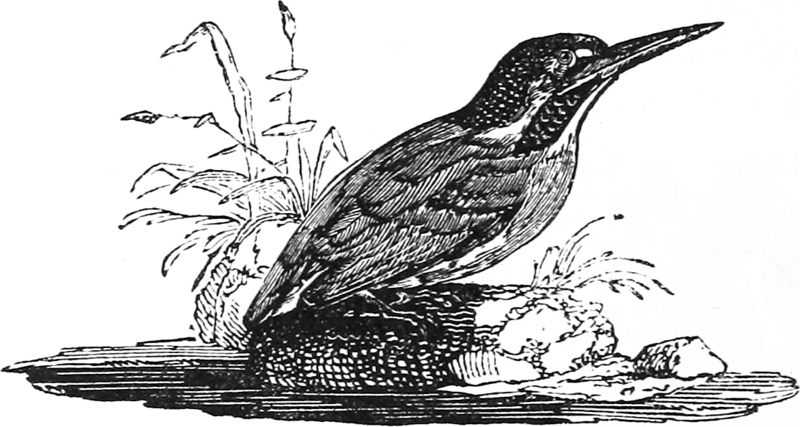
\includegraphics[scale=0.35]{images/Alycon.png}
        \end{figure}
        \vspace{0.5cm}
        \Huge
        \textbf{\textsc{Matematyka Dyskretna}}
        
        \vspace{0.5cm}
        \Large
        \textsc{Wybrane Dowody}
        
        \normalsize
        
        
        \line(1,0){330}
        
        \vspace{1cm}
        \textit{,,Myślę, że 7 punktów na 20 to nie jest zły wynik''}
        \vspace{1cm}

        \textit{\textsc{Popełnione przez}}\\
        \vspace{5mm}

        \textbf{\textsc{Dziurawy Ponton \\ Załatany Ponton \\ Puchaty Pompon \\ Zatopiony Ponton \\ Tonący Ponton \\ Notnop}}

        \vfill

        Kraków \\
        Anno Domini 2023
        
    \end{center}
    
\end{titlepage}


\tableofcontents
\section*{Licencja}
    \begin{figure}[h]
    	\begin{minipage}[c]{0.25\textwidth}
    		
\includegraphics[width=0.7\textwidth]{images/licencja.png}
    	\end{minipage}\hfill
    	\begin{minipage}[c]{0.75\textwidth}
    		\caption*{
    			Ten utwór jest dostępny na 
    			\href{https://creativecommons.org/licenses/by-sa/4.0/}{licencji Creative Commons Uznanie autorstwa
    			na tych samych warunkach 4.0 Międzynarodowe.}
    		}
    	\end{minipage}
    \end{figure}

% Actual content
\mainmatter

\chapter{Kombinatoryka}
 % Żeby nie było syfu to kolejne sekcje dodajemy do chapters/
% A potem includujemy za pomocą \input{chapters/...}

% Używamy \( \) i \[ \] zamiast dolarów -- tak jak się robi w LaTeXu


\documentclass[12pt, a4paper, polish, openany]{book}

% Please, let's familiarize ourselves with notatki.sty and tcs.sty so that we don't reinvent the wheel
\usepackage{notatki}

\fancyhead[L]{\textbf{\textit{MD}}}
\author{
}
\title{TCS and shitposting}


\begin{document}

% Front page and table of contents
\frontmatter

\input{titlepage}

\tableofcontents
\input{license}

% Actual content
\mainmatter

\chapter{Kombinatoryka}
\input{chapters/combinatorics/main}

\chapter{Zasada włączeń i wyłączeń}
\input{chapters/exclusion-inclusion/main}

\chapter{Posety}
\input{chapters/posets/main}

\chapter{Twierdzenie Ramseya}
\input{chapters/ramsey/main}

\chapter{Funkcje tworzące}
\input{chapters/generating_functions/main}

\chapter{Przepływy}
\input{chapters/flows/main}

\chapter{Skojarzenia}
\input{chapters/matchings/main}

\chapter{Kolorowanie grafów}
\input{chapters/graph-coloring/main}

\chapter{Grafy, ale nie kolorowanie}
\input{chapters/graph-misc/main}

\end{document}

\chapter{Zasada włączeń i wyłączeń}
 % Żeby nie było syfu to kolejne sekcje dodajemy do chapters/
% A potem includujemy za pomocą \input{chapters/...}

% Używamy \( \) i \[ \] zamiast dolarów -- tak jak się robi w LaTeXu


\documentclass[12pt, a4paper, polish, openany]{book}

% Please, let's familiarize ourselves with notatki.sty and tcs.sty so that we don't reinvent the wheel
\usepackage{notatki}

\fancyhead[L]{\textbf{\textit{MD}}}
\author{
}
\title{TCS and shitposting}


\begin{document}

% Front page and table of contents
\frontmatter

\input{titlepage}

\tableofcontents
\input{license}

% Actual content
\mainmatter

\chapter{Kombinatoryka}
\input{chapters/combinatorics/main}

\chapter{Zasada włączeń i wyłączeń}
\input{chapters/exclusion-inclusion/main}

\chapter{Posety}
\input{chapters/posets/main}

\chapter{Twierdzenie Ramseya}
\input{chapters/ramsey/main}

\chapter{Funkcje tworzące}
\input{chapters/generating_functions/main}

\chapter{Przepływy}
\input{chapters/flows/main}

\chapter{Skojarzenia}
\input{chapters/matchings/main}

\chapter{Kolorowanie grafów}
\input{chapters/graph-coloring/main}

\chapter{Grafy, ale nie kolorowanie}
\input{chapters/graph-misc/main}

\end{document}

\chapter{Posety}
 % Żeby nie było syfu to kolejne sekcje dodajemy do chapters/
% A potem includujemy za pomocą \input{chapters/...}

% Używamy \( \) i \[ \] zamiast dolarów -- tak jak się robi w LaTeXu


\documentclass[12pt, a4paper, polish, openany]{book}

% Please, let's familiarize ourselves with notatki.sty and tcs.sty so that we don't reinvent the wheel
\usepackage{notatki}

\fancyhead[L]{\textbf{\textit{MD}}}
\author{
}
\title{TCS and shitposting}


\begin{document}

% Front page and table of contents
\frontmatter

\input{titlepage}

\tableofcontents
\input{license}

% Actual content
\mainmatter

\chapter{Kombinatoryka}
\input{chapters/combinatorics/main}

\chapter{Zasada włączeń i wyłączeń}
\input{chapters/exclusion-inclusion/main}

\chapter{Posety}
\input{chapters/posets/main}

\chapter{Twierdzenie Ramseya}
\input{chapters/ramsey/main}

\chapter{Funkcje tworzące}
\input{chapters/generating_functions/main}

\chapter{Przepływy}
\input{chapters/flows/main}

\chapter{Skojarzenia}
\input{chapters/matchings/main}

\chapter{Kolorowanie grafów}
\input{chapters/graph-coloring/main}

\chapter{Grafy, ale nie kolorowanie}
\input{chapters/graph-misc/main}

\end{document}

\chapter{Twierdzenie Ramseya}
 % Żeby nie było syfu to kolejne sekcje dodajemy do chapters/
% A potem includujemy za pomocą \input{chapters/...}

% Używamy \( \) i \[ \] zamiast dolarów -- tak jak się robi w LaTeXu


\documentclass[12pt, a4paper, polish, openany]{book}

% Please, let's familiarize ourselves with notatki.sty and tcs.sty so that we don't reinvent the wheel
\usepackage{notatki}

\fancyhead[L]{\textbf{\textit{MD}}}
\author{
}
\title{TCS and shitposting}


\begin{document}

% Front page and table of contents
\frontmatter

\input{titlepage}

\tableofcontents
\input{license}

% Actual content
\mainmatter

\chapter{Kombinatoryka}
\input{chapters/combinatorics/main}

\chapter{Zasada włączeń i wyłączeń}
\input{chapters/exclusion-inclusion/main}

\chapter{Posety}
\input{chapters/posets/main}

\chapter{Twierdzenie Ramseya}
\input{chapters/ramsey/main}

\chapter{Funkcje tworzące}
\input{chapters/generating_functions/main}

\chapter{Przepływy}
\input{chapters/flows/main}

\chapter{Skojarzenia}
\input{chapters/matchings/main}

\chapter{Kolorowanie grafów}
\input{chapters/graph-coloring/main}

\chapter{Grafy, ale nie kolorowanie}
\input{chapters/graph-misc/main}

\end{document}

\chapter{Funkcje tworzące}
 % Żeby nie było syfu to kolejne sekcje dodajemy do chapters/
% A potem includujemy za pomocą \input{chapters/...}

% Używamy \( \) i \[ \] zamiast dolarów -- tak jak się robi w LaTeXu


\documentclass[12pt, a4paper, polish, openany]{book}

% Please, let's familiarize ourselves with notatki.sty and tcs.sty so that we don't reinvent the wheel
\usepackage{notatki}

\fancyhead[L]{\textbf{\textit{MD}}}
\author{
}
\title{TCS and shitposting}


\begin{document}

% Front page and table of contents
\frontmatter

\input{titlepage}

\tableofcontents
\input{license}

% Actual content
\mainmatter

\chapter{Kombinatoryka}
\input{chapters/combinatorics/main}

\chapter{Zasada włączeń i wyłączeń}
\input{chapters/exclusion-inclusion/main}

\chapter{Posety}
\input{chapters/posets/main}

\chapter{Twierdzenie Ramseya}
\input{chapters/ramsey/main}

\chapter{Funkcje tworzące}
\input{chapters/generating_functions/main}

\chapter{Przepływy}
\input{chapters/flows/main}

\chapter{Skojarzenia}
\input{chapters/matchings/main}

\chapter{Kolorowanie grafów}
\input{chapters/graph-coloring/main}

\chapter{Grafy, ale nie kolorowanie}
\input{chapters/graph-misc/main}

\end{document}

\chapter{Przepływy}
 % Żeby nie było syfu to kolejne sekcje dodajemy do chapters/
% A potem includujemy za pomocą \input{chapters/...}

% Używamy \( \) i \[ \] zamiast dolarów -- tak jak się robi w LaTeXu


\documentclass[12pt, a4paper, polish, openany]{book}

% Please, let's familiarize ourselves with notatki.sty and tcs.sty so that we don't reinvent the wheel
\usepackage{notatki}

\fancyhead[L]{\textbf{\textit{MD}}}
\author{
}
\title{TCS and shitposting}


\begin{document}

% Front page and table of contents
\frontmatter

\input{titlepage}

\tableofcontents
\input{license}

% Actual content
\mainmatter

\chapter{Kombinatoryka}
\input{chapters/combinatorics/main}

\chapter{Zasada włączeń i wyłączeń}
\input{chapters/exclusion-inclusion/main}

\chapter{Posety}
\input{chapters/posets/main}

\chapter{Twierdzenie Ramseya}
\input{chapters/ramsey/main}

\chapter{Funkcje tworzące}
\input{chapters/generating_functions/main}

\chapter{Przepływy}
\input{chapters/flows/main}

\chapter{Skojarzenia}
\input{chapters/matchings/main}

\chapter{Kolorowanie grafów}
\input{chapters/graph-coloring/main}

\chapter{Grafy, ale nie kolorowanie}
\input{chapters/graph-misc/main}

\end{document}

\chapter{Skojarzenia}
 % Żeby nie było syfu to kolejne sekcje dodajemy do chapters/
% A potem includujemy za pomocą \input{chapters/...}

% Używamy \( \) i \[ \] zamiast dolarów -- tak jak się robi w LaTeXu


\documentclass[12pt, a4paper, polish, openany]{book}

% Please, let's familiarize ourselves with notatki.sty and tcs.sty so that we don't reinvent the wheel
\usepackage{notatki}

\fancyhead[L]{\textbf{\textit{MD}}}
\author{
}
\title{TCS and shitposting}


\begin{document}

% Front page and table of contents
\frontmatter

\input{titlepage}

\tableofcontents
\input{license}

% Actual content
\mainmatter

\chapter{Kombinatoryka}
\input{chapters/combinatorics/main}

\chapter{Zasada włączeń i wyłączeń}
\input{chapters/exclusion-inclusion/main}

\chapter{Posety}
\input{chapters/posets/main}

\chapter{Twierdzenie Ramseya}
\input{chapters/ramsey/main}

\chapter{Funkcje tworzące}
\input{chapters/generating_functions/main}

\chapter{Przepływy}
\input{chapters/flows/main}

\chapter{Skojarzenia}
\input{chapters/matchings/main}

\chapter{Kolorowanie grafów}
\input{chapters/graph-coloring/main}

\chapter{Grafy, ale nie kolorowanie}
\input{chapters/graph-misc/main}

\end{document}

\chapter{Kolorowanie grafów}
 % Żeby nie było syfu to kolejne sekcje dodajemy do chapters/
% A potem includujemy za pomocą \input{chapters/...}

% Używamy \( \) i \[ \] zamiast dolarów -- tak jak się robi w LaTeXu


\documentclass[12pt, a4paper, polish, openany]{book}

% Please, let's familiarize ourselves with notatki.sty and tcs.sty so that we don't reinvent the wheel
\usepackage{notatki}

\fancyhead[L]{\textbf{\textit{MD}}}
\author{
}
\title{TCS and shitposting}


\begin{document}

% Front page and table of contents
\frontmatter

\input{titlepage}

\tableofcontents
\input{license}

% Actual content
\mainmatter

\chapter{Kombinatoryka}
\input{chapters/combinatorics/main}

\chapter{Zasada włączeń i wyłączeń}
\input{chapters/exclusion-inclusion/main}

\chapter{Posety}
\input{chapters/posets/main}

\chapter{Twierdzenie Ramseya}
\input{chapters/ramsey/main}

\chapter{Funkcje tworzące}
\input{chapters/generating_functions/main}

\chapter{Przepływy}
\input{chapters/flows/main}

\chapter{Skojarzenia}
\input{chapters/matchings/main}

\chapter{Kolorowanie grafów}
\input{chapters/graph-coloring/main}

\chapter{Grafy, ale nie kolorowanie}
\input{chapters/graph-misc/main}

\end{document}

\chapter{Grafy, ale nie kolorowanie}
 % Żeby nie było syfu to kolejne sekcje dodajemy do chapters/
% A potem includujemy za pomocą \input{chapters/...}

% Używamy \( \) i \[ \] zamiast dolarów -- tak jak się robi w LaTeXu


\documentclass[12pt, a4paper, polish, openany]{book}

% Please, let's familiarize ourselves with notatki.sty and tcs.sty so that we don't reinvent the wheel
\usepackage{notatki}

\fancyhead[L]{\textbf{\textit{MD}}}
\author{
}
\title{TCS and shitposting}


\begin{document}

% Front page and table of contents
\frontmatter

\input{titlepage}

\tableofcontents
\input{license}

% Actual content
\mainmatter

\chapter{Kombinatoryka}
\input{chapters/combinatorics/main}

\chapter{Zasada włączeń i wyłączeń}
\input{chapters/exclusion-inclusion/main}

\chapter{Posety}
\input{chapters/posets/main}

\chapter{Twierdzenie Ramseya}
\input{chapters/ramsey/main}

\chapter{Funkcje tworzące}
\input{chapters/generating_functions/main}

\chapter{Przepływy}
\input{chapters/flows/main}

\chapter{Skojarzenia}
\input{chapters/matchings/main}

\chapter{Kolorowanie grafów}
\input{chapters/graph-coloring/main}

\chapter{Grafy, ale nie kolorowanie}
\input{chapters/graph-misc/main}

\end{document}

\end{document}

\chapter{Twierdzenie Ramseya}
 % Żeby nie było syfu to kolejne sekcje dodajemy do chapters/
% A potem includujemy za pomocą \input{chapters/...}

% Używamy \( \) i \[ \] zamiast dolarów -- tak jak się robi w LaTeXu


\documentclass[12pt, a4paper, polish, openany]{book}

% Please, let's familiarize ourselves with notatki.sty and tcs.sty so that we don't reinvent the wheel
\usepackage{notatki}

\fancyhead[L]{\textbf{\textit{MD}}}
\author{
}
\title{TCS and shitposting}


\begin{document}

% Front page and table of contents
\frontmatter

\begin{titlepage} 

    \begin{center}
         \begin{figure}[h]
            \centering
            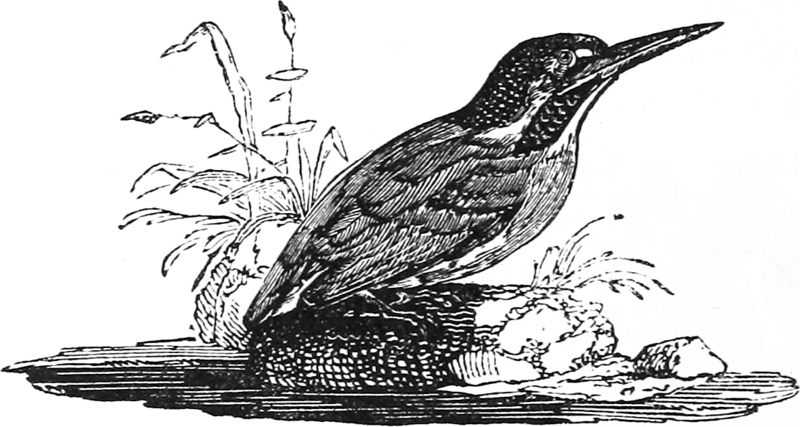
\includegraphics[scale=0.35]{images/Alycon.png}
        \end{figure}
        \vspace{0.5cm}
        \Huge
        \textbf{\textsc{Matematyka Dyskretna}}
        
        \vspace{0.5cm}
        \Large
        \textsc{Wybrane Dowody}
        
        \normalsize
        
        
        \line(1,0){330}
        
        \vspace{1cm}
        \textit{,,Myślę, że 7 punktów na 20 to nie jest zły wynik''}
        \vspace{1cm}

        \textit{\textsc{Popełnione przez}}\\
        \vspace{5mm}

        \textbf{\textsc{Dziurawy Ponton \\ Załatany Ponton \\ Puchaty Pompon \\ Zatopiony Ponton \\ Tonący Ponton \\ Notnop}}

        \vfill

        Kraków \\
        Anno Domini 2023
        
    \end{center}
    
\end{titlepage}


\tableofcontents
\section*{Licencja}
    \begin{figure}[h]
    	\begin{minipage}[c]{0.25\textwidth}
    		
\includegraphics[width=0.7\textwidth]{images/licencja.png}
    	\end{minipage}\hfill
    	\begin{minipage}[c]{0.75\textwidth}
    		\caption*{
    			Ten utwór jest dostępny na 
    			\href{https://creativecommons.org/licenses/by-sa/4.0/}{licencji Creative Commons Uznanie autorstwa
    			na tych samych warunkach 4.0 Międzynarodowe.}
    		}
    	\end{minipage}
    \end{figure}

% Actual content
\mainmatter

\chapter{Kombinatoryka}
 % Żeby nie było syfu to kolejne sekcje dodajemy do chapters/
% A potem includujemy za pomocą \input{chapters/...}

% Używamy \( \) i \[ \] zamiast dolarów -- tak jak się robi w LaTeXu


\documentclass[12pt, a4paper, polish, openany]{book}

% Please, let's familiarize ourselves with notatki.sty and tcs.sty so that we don't reinvent the wheel
\usepackage{notatki}

\fancyhead[L]{\textbf{\textit{MD}}}
\author{
}
\title{TCS and shitposting}


\begin{document}

% Front page and table of contents
\frontmatter

\input{titlepage}

\tableofcontents
\input{license}

% Actual content
\mainmatter

\chapter{Kombinatoryka}
\input{chapters/combinatorics/main}

\chapter{Zasada włączeń i wyłączeń}
\input{chapters/exclusion-inclusion/main}

\chapter{Posety}
\input{chapters/posets/main}

\chapter{Twierdzenie Ramseya}
\input{chapters/ramsey/main}

\chapter{Funkcje tworzące}
\input{chapters/generating_functions/main}

\chapter{Przepływy}
\input{chapters/flows/main}

\chapter{Skojarzenia}
\input{chapters/matchings/main}

\chapter{Kolorowanie grafów}
\input{chapters/graph-coloring/main}

\chapter{Grafy, ale nie kolorowanie}
\input{chapters/graph-misc/main}

\end{document}

\chapter{Zasada włączeń i wyłączeń}
 % Żeby nie było syfu to kolejne sekcje dodajemy do chapters/
% A potem includujemy za pomocą \input{chapters/...}

% Używamy \( \) i \[ \] zamiast dolarów -- tak jak się robi w LaTeXu


\documentclass[12pt, a4paper, polish, openany]{book}

% Please, let's familiarize ourselves with notatki.sty and tcs.sty so that we don't reinvent the wheel
\usepackage{notatki}

\fancyhead[L]{\textbf{\textit{MD}}}
\author{
}
\title{TCS and shitposting}


\begin{document}

% Front page and table of contents
\frontmatter

\input{titlepage}

\tableofcontents
\input{license}

% Actual content
\mainmatter

\chapter{Kombinatoryka}
\input{chapters/combinatorics/main}

\chapter{Zasada włączeń i wyłączeń}
\input{chapters/exclusion-inclusion/main}

\chapter{Posety}
\input{chapters/posets/main}

\chapter{Twierdzenie Ramseya}
\input{chapters/ramsey/main}

\chapter{Funkcje tworzące}
\input{chapters/generating_functions/main}

\chapter{Przepływy}
\input{chapters/flows/main}

\chapter{Skojarzenia}
\input{chapters/matchings/main}

\chapter{Kolorowanie grafów}
\input{chapters/graph-coloring/main}

\chapter{Grafy, ale nie kolorowanie}
\input{chapters/graph-misc/main}

\end{document}

\chapter{Posety}
 % Żeby nie było syfu to kolejne sekcje dodajemy do chapters/
% A potem includujemy za pomocą \input{chapters/...}

% Używamy \( \) i \[ \] zamiast dolarów -- tak jak się robi w LaTeXu


\documentclass[12pt, a4paper, polish, openany]{book}

% Please, let's familiarize ourselves with notatki.sty and tcs.sty so that we don't reinvent the wheel
\usepackage{notatki}

\fancyhead[L]{\textbf{\textit{MD}}}
\author{
}
\title{TCS and shitposting}


\begin{document}

% Front page and table of contents
\frontmatter

\input{titlepage}

\tableofcontents
\input{license}

% Actual content
\mainmatter

\chapter{Kombinatoryka}
\input{chapters/combinatorics/main}

\chapter{Zasada włączeń i wyłączeń}
\input{chapters/exclusion-inclusion/main}

\chapter{Posety}
\input{chapters/posets/main}

\chapter{Twierdzenie Ramseya}
\input{chapters/ramsey/main}

\chapter{Funkcje tworzące}
\input{chapters/generating_functions/main}

\chapter{Przepływy}
\input{chapters/flows/main}

\chapter{Skojarzenia}
\input{chapters/matchings/main}

\chapter{Kolorowanie grafów}
\input{chapters/graph-coloring/main}

\chapter{Grafy, ale nie kolorowanie}
\input{chapters/graph-misc/main}

\end{document}

\chapter{Twierdzenie Ramseya}
 % Żeby nie było syfu to kolejne sekcje dodajemy do chapters/
% A potem includujemy za pomocą \input{chapters/...}

% Używamy \( \) i \[ \] zamiast dolarów -- tak jak się robi w LaTeXu


\documentclass[12pt, a4paper, polish, openany]{book}

% Please, let's familiarize ourselves with notatki.sty and tcs.sty so that we don't reinvent the wheel
\usepackage{notatki}

\fancyhead[L]{\textbf{\textit{MD}}}
\author{
}
\title{TCS and shitposting}


\begin{document}

% Front page and table of contents
\frontmatter

\input{titlepage}

\tableofcontents
\input{license}

% Actual content
\mainmatter

\chapter{Kombinatoryka}
\input{chapters/combinatorics/main}

\chapter{Zasada włączeń i wyłączeń}
\input{chapters/exclusion-inclusion/main}

\chapter{Posety}
\input{chapters/posets/main}

\chapter{Twierdzenie Ramseya}
\input{chapters/ramsey/main}

\chapter{Funkcje tworzące}
\input{chapters/generating_functions/main}

\chapter{Przepływy}
\input{chapters/flows/main}

\chapter{Skojarzenia}
\input{chapters/matchings/main}

\chapter{Kolorowanie grafów}
\input{chapters/graph-coloring/main}

\chapter{Grafy, ale nie kolorowanie}
\input{chapters/graph-misc/main}

\end{document}

\chapter{Funkcje tworzące}
 % Żeby nie było syfu to kolejne sekcje dodajemy do chapters/
% A potem includujemy za pomocą \input{chapters/...}

% Używamy \( \) i \[ \] zamiast dolarów -- tak jak się robi w LaTeXu


\documentclass[12pt, a4paper, polish, openany]{book}

% Please, let's familiarize ourselves with notatki.sty and tcs.sty so that we don't reinvent the wheel
\usepackage{notatki}

\fancyhead[L]{\textbf{\textit{MD}}}
\author{
}
\title{TCS and shitposting}


\begin{document}

% Front page and table of contents
\frontmatter

\input{titlepage}

\tableofcontents
\input{license}

% Actual content
\mainmatter

\chapter{Kombinatoryka}
\input{chapters/combinatorics/main}

\chapter{Zasada włączeń i wyłączeń}
\input{chapters/exclusion-inclusion/main}

\chapter{Posety}
\input{chapters/posets/main}

\chapter{Twierdzenie Ramseya}
\input{chapters/ramsey/main}

\chapter{Funkcje tworzące}
\input{chapters/generating_functions/main}

\chapter{Przepływy}
\input{chapters/flows/main}

\chapter{Skojarzenia}
\input{chapters/matchings/main}

\chapter{Kolorowanie grafów}
\input{chapters/graph-coloring/main}

\chapter{Grafy, ale nie kolorowanie}
\input{chapters/graph-misc/main}

\end{document}

\chapter{Przepływy}
 % Żeby nie było syfu to kolejne sekcje dodajemy do chapters/
% A potem includujemy za pomocą \input{chapters/...}

% Używamy \( \) i \[ \] zamiast dolarów -- tak jak się robi w LaTeXu


\documentclass[12pt, a4paper, polish, openany]{book}

% Please, let's familiarize ourselves with notatki.sty and tcs.sty so that we don't reinvent the wheel
\usepackage{notatki}

\fancyhead[L]{\textbf{\textit{MD}}}
\author{
}
\title{TCS and shitposting}


\begin{document}

% Front page and table of contents
\frontmatter

\input{titlepage}

\tableofcontents
\input{license}

% Actual content
\mainmatter

\chapter{Kombinatoryka}
\input{chapters/combinatorics/main}

\chapter{Zasada włączeń i wyłączeń}
\input{chapters/exclusion-inclusion/main}

\chapter{Posety}
\input{chapters/posets/main}

\chapter{Twierdzenie Ramseya}
\input{chapters/ramsey/main}

\chapter{Funkcje tworzące}
\input{chapters/generating_functions/main}

\chapter{Przepływy}
\input{chapters/flows/main}

\chapter{Skojarzenia}
\input{chapters/matchings/main}

\chapter{Kolorowanie grafów}
\input{chapters/graph-coloring/main}

\chapter{Grafy, ale nie kolorowanie}
\input{chapters/graph-misc/main}

\end{document}

\chapter{Skojarzenia}
 % Żeby nie było syfu to kolejne sekcje dodajemy do chapters/
% A potem includujemy za pomocą \input{chapters/...}

% Używamy \( \) i \[ \] zamiast dolarów -- tak jak się robi w LaTeXu


\documentclass[12pt, a4paper, polish, openany]{book}

% Please, let's familiarize ourselves with notatki.sty and tcs.sty so that we don't reinvent the wheel
\usepackage{notatki}

\fancyhead[L]{\textbf{\textit{MD}}}
\author{
}
\title{TCS and shitposting}


\begin{document}

% Front page and table of contents
\frontmatter

\input{titlepage}

\tableofcontents
\input{license}

% Actual content
\mainmatter

\chapter{Kombinatoryka}
\input{chapters/combinatorics/main}

\chapter{Zasada włączeń i wyłączeń}
\input{chapters/exclusion-inclusion/main}

\chapter{Posety}
\input{chapters/posets/main}

\chapter{Twierdzenie Ramseya}
\input{chapters/ramsey/main}

\chapter{Funkcje tworzące}
\input{chapters/generating_functions/main}

\chapter{Przepływy}
\input{chapters/flows/main}

\chapter{Skojarzenia}
\input{chapters/matchings/main}

\chapter{Kolorowanie grafów}
\input{chapters/graph-coloring/main}

\chapter{Grafy, ale nie kolorowanie}
\input{chapters/graph-misc/main}

\end{document}

\chapter{Kolorowanie grafów}
 % Żeby nie było syfu to kolejne sekcje dodajemy do chapters/
% A potem includujemy za pomocą \input{chapters/...}

% Używamy \( \) i \[ \] zamiast dolarów -- tak jak się robi w LaTeXu


\documentclass[12pt, a4paper, polish, openany]{book}

% Please, let's familiarize ourselves with notatki.sty and tcs.sty so that we don't reinvent the wheel
\usepackage{notatki}

\fancyhead[L]{\textbf{\textit{MD}}}
\author{
}
\title{TCS and shitposting}


\begin{document}

% Front page and table of contents
\frontmatter

\input{titlepage}

\tableofcontents
\input{license}

% Actual content
\mainmatter

\chapter{Kombinatoryka}
\input{chapters/combinatorics/main}

\chapter{Zasada włączeń i wyłączeń}
\input{chapters/exclusion-inclusion/main}

\chapter{Posety}
\input{chapters/posets/main}

\chapter{Twierdzenie Ramseya}
\input{chapters/ramsey/main}

\chapter{Funkcje tworzące}
\input{chapters/generating_functions/main}

\chapter{Przepływy}
\input{chapters/flows/main}

\chapter{Skojarzenia}
\input{chapters/matchings/main}

\chapter{Kolorowanie grafów}
\input{chapters/graph-coloring/main}

\chapter{Grafy, ale nie kolorowanie}
\input{chapters/graph-misc/main}

\end{document}

\chapter{Grafy, ale nie kolorowanie}
 % Żeby nie było syfu to kolejne sekcje dodajemy do chapters/
% A potem includujemy za pomocą \input{chapters/...}

% Używamy \( \) i \[ \] zamiast dolarów -- tak jak się robi w LaTeXu


\documentclass[12pt, a4paper, polish, openany]{book}

% Please, let's familiarize ourselves with notatki.sty and tcs.sty so that we don't reinvent the wheel
\usepackage{notatki}

\fancyhead[L]{\textbf{\textit{MD}}}
\author{
}
\title{TCS and shitposting}


\begin{document}

% Front page and table of contents
\frontmatter

\input{titlepage}

\tableofcontents
\input{license}

% Actual content
\mainmatter

\chapter{Kombinatoryka}
\input{chapters/combinatorics/main}

\chapter{Zasada włączeń i wyłączeń}
\input{chapters/exclusion-inclusion/main}

\chapter{Posety}
\input{chapters/posets/main}

\chapter{Twierdzenie Ramseya}
\input{chapters/ramsey/main}

\chapter{Funkcje tworzące}
\input{chapters/generating_functions/main}

\chapter{Przepływy}
\input{chapters/flows/main}

\chapter{Skojarzenia}
\input{chapters/matchings/main}

\chapter{Kolorowanie grafów}
\input{chapters/graph-coloring/main}

\chapter{Grafy, ale nie kolorowanie}
\input{chapters/graph-misc/main}

\end{document}

\end{document}

\chapter{Funkcje tworzące}
 % Żeby nie było syfu to kolejne sekcje dodajemy do chapters/
% A potem includujemy za pomocą \input{chapters/...}

% Używamy \( \) i \[ \] zamiast dolarów -- tak jak się robi w LaTeXu


\documentclass[12pt, a4paper, polish, openany]{book}

% Please, let's familiarize ourselves with notatki.sty and tcs.sty so that we don't reinvent the wheel
\usepackage{notatki}

\fancyhead[L]{\textbf{\textit{MD}}}
\author{
}
\title{TCS and shitposting}


\begin{document}

% Front page and table of contents
\frontmatter

\begin{titlepage} 

    \begin{center}
         \begin{figure}[h]
            \centering
            \includegraphics[scale=0.35]{images/Alycon.png}
        \end{figure}
        \vspace{0.5cm}
        \Huge
        \textbf{\textsc{Matematyka Dyskretna}}
        
        \vspace{0.5cm}
        \Large
        \textsc{Wybrane Dowody}
        
        \normalsize
        
        
        \line(1,0){330}
        
        \vspace{1cm}
        \textit{,,Myślę, że 7 punktów na 20 to nie jest zły wynik''}
        \vspace{1cm}

        \textit{\textsc{Popełnione przez}}\\
        \vspace{5mm}

        \textbf{\textsc{Dziurawy Ponton \\ Załatany Ponton \\ Puchaty Pompon \\ Zatopiony Ponton \\ Tonący Ponton \\ Notnop}}

        \vfill

        Kraków \\
        Anno Domini 2023
        
    \end{center}
    
\end{titlepage}


\tableofcontents
\section*{Licencja}
    \begin{figure}[h]
    	\begin{minipage}[c]{0.25\textwidth}
    		\includegraphics[width=0.7\textwidth]{images/licencja.png}
    	\end{minipage}\hfill
    	\begin{minipage}[c]{0.75\textwidth}
    		\caption*{
    			Ten utwór jest dostępny na 
    			\href{https://creativecommons.org/licenses/by-sa/4.0/}{licencji Creative Commons Uznanie autorstwa
    			na tych samych warunkach 4.0 Międzynarodowe.}
    		}
    	\end{minipage}
    \end{figure}

% Actual content
\mainmatter

\chapter{Kombinatoryka}
 % Żeby nie było syfu to kolejne sekcje dodajemy do chapters/
% A potem includujemy za pomocą \input{chapters/...}

% Używamy \( \) i \[ \] zamiast dolarów -- tak jak się robi w LaTeXu


\documentclass[12pt, a4paper, polish, openany]{book}

% Please, let's familiarize ourselves with notatki.sty and tcs.sty so that we don't reinvent the wheel
\usepackage{notatki}

\fancyhead[L]{\textbf{\textit{MD}}}
\author{
}
\title{TCS and shitposting}


\begin{document}

% Front page and table of contents
\frontmatter

\input{titlepage}

\tableofcontents
\input{license}

% Actual content
\mainmatter

\chapter{Kombinatoryka}
\input{chapters/combinatorics/main}

\chapter{Zasada włączeń i wyłączeń}
\input{chapters/exclusion-inclusion/main}

\chapter{Posety}
\input{chapters/posets/main}

\chapter{Twierdzenie Ramseya}
\input{chapters/ramsey/main}

\chapter{Funkcje tworzące}
\input{chapters/generating_functions/main}

\chapter{Przepływy}
\input{chapters/flows/main}

\chapter{Skojarzenia}
\input{chapters/matchings/main}

\chapter{Kolorowanie grafów}
\input{chapters/graph-coloring/main}

\chapter{Grafy, ale nie kolorowanie}
\input{chapters/graph-misc/main}

\end{document}

\chapter{Zasada włączeń i wyłączeń}
 % Żeby nie było syfu to kolejne sekcje dodajemy do chapters/
% A potem includujemy za pomocą \input{chapters/...}

% Używamy \( \) i \[ \] zamiast dolarów -- tak jak się robi w LaTeXu


\documentclass[12pt, a4paper, polish, openany]{book}

% Please, let's familiarize ourselves with notatki.sty and tcs.sty so that we don't reinvent the wheel
\usepackage{notatki}

\fancyhead[L]{\textbf{\textit{MD}}}
\author{
}
\title{TCS and shitposting}


\begin{document}

% Front page and table of contents
\frontmatter

\input{titlepage}

\tableofcontents
\input{license}

% Actual content
\mainmatter

\chapter{Kombinatoryka}
\input{chapters/combinatorics/main}

\chapter{Zasada włączeń i wyłączeń}
\input{chapters/exclusion-inclusion/main}

\chapter{Posety}
\input{chapters/posets/main}

\chapter{Twierdzenie Ramseya}
\input{chapters/ramsey/main}

\chapter{Funkcje tworzące}
\input{chapters/generating_functions/main}

\chapter{Przepływy}
\input{chapters/flows/main}

\chapter{Skojarzenia}
\input{chapters/matchings/main}

\chapter{Kolorowanie grafów}
\input{chapters/graph-coloring/main}

\chapter{Grafy, ale nie kolorowanie}
\input{chapters/graph-misc/main}

\end{document}

\chapter{Posety}
 % Żeby nie było syfu to kolejne sekcje dodajemy do chapters/
% A potem includujemy za pomocą \input{chapters/...}

% Używamy \( \) i \[ \] zamiast dolarów -- tak jak się robi w LaTeXu


\documentclass[12pt, a4paper, polish, openany]{book}

% Please, let's familiarize ourselves with notatki.sty and tcs.sty so that we don't reinvent the wheel
\usepackage{notatki}

\fancyhead[L]{\textbf{\textit{MD}}}
\author{
}
\title{TCS and shitposting}


\begin{document}

% Front page and table of contents
\frontmatter

\input{titlepage}

\tableofcontents
\input{license}

% Actual content
\mainmatter

\chapter{Kombinatoryka}
\input{chapters/combinatorics/main}

\chapter{Zasada włączeń i wyłączeń}
\input{chapters/exclusion-inclusion/main}

\chapter{Posety}
\input{chapters/posets/main}

\chapter{Twierdzenie Ramseya}
\input{chapters/ramsey/main}

\chapter{Funkcje tworzące}
\input{chapters/generating_functions/main}

\chapter{Przepływy}
\input{chapters/flows/main}

\chapter{Skojarzenia}
\input{chapters/matchings/main}

\chapter{Kolorowanie grafów}
\input{chapters/graph-coloring/main}

\chapter{Grafy, ale nie kolorowanie}
\input{chapters/graph-misc/main}

\end{document}

\chapter{Twierdzenie Ramseya}
 % Żeby nie było syfu to kolejne sekcje dodajemy do chapters/
% A potem includujemy za pomocą \input{chapters/...}

% Używamy \( \) i \[ \] zamiast dolarów -- tak jak się robi w LaTeXu


\documentclass[12pt, a4paper, polish, openany]{book}

% Please, let's familiarize ourselves with notatki.sty and tcs.sty so that we don't reinvent the wheel
\usepackage{notatki}

\fancyhead[L]{\textbf{\textit{MD}}}
\author{
}
\title{TCS and shitposting}


\begin{document}

% Front page and table of contents
\frontmatter

\input{titlepage}

\tableofcontents
\input{license}

% Actual content
\mainmatter

\chapter{Kombinatoryka}
\input{chapters/combinatorics/main}

\chapter{Zasada włączeń i wyłączeń}
\input{chapters/exclusion-inclusion/main}

\chapter{Posety}
\input{chapters/posets/main}

\chapter{Twierdzenie Ramseya}
\input{chapters/ramsey/main}

\chapter{Funkcje tworzące}
\input{chapters/generating_functions/main}

\chapter{Przepływy}
\input{chapters/flows/main}

\chapter{Skojarzenia}
\input{chapters/matchings/main}

\chapter{Kolorowanie grafów}
\input{chapters/graph-coloring/main}

\chapter{Grafy, ale nie kolorowanie}
\input{chapters/graph-misc/main}

\end{document}

\chapter{Funkcje tworzące}
 % Żeby nie było syfu to kolejne sekcje dodajemy do chapters/
% A potem includujemy za pomocą \input{chapters/...}

% Używamy \( \) i \[ \] zamiast dolarów -- tak jak się robi w LaTeXu


\documentclass[12pt, a4paper, polish, openany]{book}

% Please, let's familiarize ourselves with notatki.sty and tcs.sty so that we don't reinvent the wheel
\usepackage{notatki}

\fancyhead[L]{\textbf{\textit{MD}}}
\author{
}
\title{TCS and shitposting}


\begin{document}

% Front page and table of contents
\frontmatter

\input{titlepage}

\tableofcontents
\input{license}

% Actual content
\mainmatter

\chapter{Kombinatoryka}
\input{chapters/combinatorics/main}

\chapter{Zasada włączeń i wyłączeń}
\input{chapters/exclusion-inclusion/main}

\chapter{Posety}
\input{chapters/posets/main}

\chapter{Twierdzenie Ramseya}
\input{chapters/ramsey/main}

\chapter{Funkcje tworzące}
\input{chapters/generating_functions/main}

\chapter{Przepływy}
\input{chapters/flows/main}

\chapter{Skojarzenia}
\input{chapters/matchings/main}

\chapter{Kolorowanie grafów}
\input{chapters/graph-coloring/main}

\chapter{Grafy, ale nie kolorowanie}
\input{chapters/graph-misc/main}

\end{document}

\chapter{Przepływy}
 % Żeby nie było syfu to kolejne sekcje dodajemy do chapters/
% A potem includujemy za pomocą \input{chapters/...}

% Używamy \( \) i \[ \] zamiast dolarów -- tak jak się robi w LaTeXu


\documentclass[12pt, a4paper, polish, openany]{book}

% Please, let's familiarize ourselves with notatki.sty and tcs.sty so that we don't reinvent the wheel
\usepackage{notatki}

\fancyhead[L]{\textbf{\textit{MD}}}
\author{
}
\title{TCS and shitposting}


\begin{document}

% Front page and table of contents
\frontmatter

\input{titlepage}

\tableofcontents
\input{license}

% Actual content
\mainmatter

\chapter{Kombinatoryka}
\input{chapters/combinatorics/main}

\chapter{Zasada włączeń i wyłączeń}
\input{chapters/exclusion-inclusion/main}

\chapter{Posety}
\input{chapters/posets/main}

\chapter{Twierdzenie Ramseya}
\input{chapters/ramsey/main}

\chapter{Funkcje tworzące}
\input{chapters/generating_functions/main}

\chapter{Przepływy}
\input{chapters/flows/main}

\chapter{Skojarzenia}
\input{chapters/matchings/main}

\chapter{Kolorowanie grafów}
\input{chapters/graph-coloring/main}

\chapter{Grafy, ale nie kolorowanie}
\input{chapters/graph-misc/main}

\end{document}

\chapter{Skojarzenia}
 % Żeby nie było syfu to kolejne sekcje dodajemy do chapters/
% A potem includujemy za pomocą \input{chapters/...}

% Używamy \( \) i \[ \] zamiast dolarów -- tak jak się robi w LaTeXu


\documentclass[12pt, a4paper, polish, openany]{book}

% Please, let's familiarize ourselves with notatki.sty and tcs.sty so that we don't reinvent the wheel
\usepackage{notatki}

\fancyhead[L]{\textbf{\textit{MD}}}
\author{
}
\title{TCS and shitposting}


\begin{document}

% Front page and table of contents
\frontmatter

\input{titlepage}

\tableofcontents
\input{license}

% Actual content
\mainmatter

\chapter{Kombinatoryka}
\input{chapters/combinatorics/main}

\chapter{Zasada włączeń i wyłączeń}
\input{chapters/exclusion-inclusion/main}

\chapter{Posety}
\input{chapters/posets/main}

\chapter{Twierdzenie Ramseya}
\input{chapters/ramsey/main}

\chapter{Funkcje tworzące}
\input{chapters/generating_functions/main}

\chapter{Przepływy}
\input{chapters/flows/main}

\chapter{Skojarzenia}
\input{chapters/matchings/main}

\chapter{Kolorowanie grafów}
\input{chapters/graph-coloring/main}

\chapter{Grafy, ale nie kolorowanie}
\input{chapters/graph-misc/main}

\end{document}

\chapter{Kolorowanie grafów}
 % Żeby nie było syfu to kolejne sekcje dodajemy do chapters/
% A potem includujemy za pomocą \input{chapters/...}

% Używamy \( \) i \[ \] zamiast dolarów -- tak jak się robi w LaTeXu


\documentclass[12pt, a4paper, polish, openany]{book}

% Please, let's familiarize ourselves with notatki.sty and tcs.sty so that we don't reinvent the wheel
\usepackage{notatki}

\fancyhead[L]{\textbf{\textit{MD}}}
\author{
}
\title{TCS and shitposting}


\begin{document}

% Front page and table of contents
\frontmatter

\input{titlepage}

\tableofcontents
\input{license}

% Actual content
\mainmatter

\chapter{Kombinatoryka}
\input{chapters/combinatorics/main}

\chapter{Zasada włączeń i wyłączeń}
\input{chapters/exclusion-inclusion/main}

\chapter{Posety}
\input{chapters/posets/main}

\chapter{Twierdzenie Ramseya}
\input{chapters/ramsey/main}

\chapter{Funkcje tworzące}
\input{chapters/generating_functions/main}

\chapter{Przepływy}
\input{chapters/flows/main}

\chapter{Skojarzenia}
\input{chapters/matchings/main}

\chapter{Kolorowanie grafów}
\input{chapters/graph-coloring/main}

\chapter{Grafy, ale nie kolorowanie}
\input{chapters/graph-misc/main}

\end{document}

\chapter{Grafy, ale nie kolorowanie}
 % Żeby nie było syfu to kolejne sekcje dodajemy do chapters/
% A potem includujemy za pomocą \input{chapters/...}

% Używamy \( \) i \[ \] zamiast dolarów -- tak jak się robi w LaTeXu


\documentclass[12pt, a4paper, polish, openany]{book}

% Please, let's familiarize ourselves with notatki.sty and tcs.sty so that we don't reinvent the wheel
\usepackage{notatki}

\fancyhead[L]{\textbf{\textit{MD}}}
\author{
}
\title{TCS and shitposting}


\begin{document}

% Front page and table of contents
\frontmatter

\input{titlepage}

\tableofcontents
\input{license}

% Actual content
\mainmatter

\chapter{Kombinatoryka}
\input{chapters/combinatorics/main}

\chapter{Zasada włączeń i wyłączeń}
\input{chapters/exclusion-inclusion/main}

\chapter{Posety}
\input{chapters/posets/main}

\chapter{Twierdzenie Ramseya}
\input{chapters/ramsey/main}

\chapter{Funkcje tworzące}
\input{chapters/generating_functions/main}

\chapter{Przepływy}
\input{chapters/flows/main}

\chapter{Skojarzenia}
\input{chapters/matchings/main}

\chapter{Kolorowanie grafów}
\input{chapters/graph-coloring/main}

\chapter{Grafy, ale nie kolorowanie}
\input{chapters/graph-misc/main}

\end{document}

\end{document}

\chapter{Przepływy}
 % Żeby nie było syfu to kolejne sekcje dodajemy do chapters/
% A potem includujemy za pomocą \input{chapters/...}

% Używamy \( \) i \[ \] zamiast dolarów -- tak jak się robi w LaTeXu


\documentclass[12pt, a4paper, polish, openany]{book}

% Please, let's familiarize ourselves with notatki.sty and tcs.sty so that we don't reinvent the wheel
\usepackage{notatki}

\fancyhead[L]{\textbf{\textit{MD}}}
\author{
}
\title{TCS and shitposting}


\begin{document}

% Front page and table of contents
\frontmatter

\begin{titlepage} 

    \begin{center}
         \begin{figure}[h]
            \centering
            \includegraphics[scale=0.35]{images/Alycon.png}
        \end{figure}
        \vspace{0.5cm}
        \Huge
        \textbf{\textsc{Matematyka Dyskretna}}
        
        \vspace{0.5cm}
        \Large
        \textsc{Wybrane Dowody}
        
        \normalsize
        
        
        \line(1,0){330}
        
        \vspace{1cm}
        \textit{,,Myślę, że 7 punktów na 20 to nie jest zły wynik''}
        \vspace{1cm}

        \textit{\textsc{Popełnione przez}}\\
        \vspace{5mm}

        \textbf{\textsc{Dziurawy Ponton \\ Załatany Ponton \\ Puchaty Pompon \\ Zatopiony Ponton \\ Tonący Ponton \\ Notnop}}

        \vfill

        Kraków \\
        Anno Domini 2023
        
    \end{center}
    
\end{titlepage}


\tableofcontents
\section*{Licencja}
    \begin{figure}[h]
    	\begin{minipage}[c]{0.25\textwidth}
    		\includegraphics[width=0.7\textwidth]{images/licencja.png}
    	\end{minipage}\hfill
    	\begin{minipage}[c]{0.75\textwidth}
    		\caption*{
    			Ten utwór jest dostępny na 
    			\href{https://creativecommons.org/licenses/by-sa/4.0/}{licencji Creative Commons Uznanie autorstwa
    			na tych samych warunkach 4.0 Międzynarodowe.}
    		}
    	\end{minipage}
    \end{figure}

% Actual content
\mainmatter

\chapter{Kombinatoryka}
 % Żeby nie było syfu to kolejne sekcje dodajemy do chapters/
% A potem includujemy za pomocą \input{chapters/...}

% Używamy \( \) i \[ \] zamiast dolarów -- tak jak się robi w LaTeXu


\documentclass[12pt, a4paper, polish, openany]{book}

% Please, let's familiarize ourselves with notatki.sty and tcs.sty so that we don't reinvent the wheel
\usepackage{notatki}

\fancyhead[L]{\textbf{\textit{MD}}}
\author{
}
\title{TCS and shitposting}


\begin{document}

% Front page and table of contents
\frontmatter

\input{titlepage}

\tableofcontents
\input{license}

% Actual content
\mainmatter

\chapter{Kombinatoryka}
\input{chapters/combinatorics/main}

\chapter{Zasada włączeń i wyłączeń}
\input{chapters/exclusion-inclusion/main}

\chapter{Posety}
\input{chapters/posets/main}

\chapter{Twierdzenie Ramseya}
\input{chapters/ramsey/main}

\chapter{Funkcje tworzące}
\input{chapters/generating_functions/main}

\chapter{Przepływy}
\input{chapters/flows/main}

\chapter{Skojarzenia}
\input{chapters/matchings/main}

\chapter{Kolorowanie grafów}
\input{chapters/graph-coloring/main}

\chapter{Grafy, ale nie kolorowanie}
\input{chapters/graph-misc/main}

\end{document}

\chapter{Zasada włączeń i wyłączeń}
 % Żeby nie było syfu to kolejne sekcje dodajemy do chapters/
% A potem includujemy za pomocą \input{chapters/...}

% Używamy \( \) i \[ \] zamiast dolarów -- tak jak się robi w LaTeXu


\documentclass[12pt, a4paper, polish, openany]{book}

% Please, let's familiarize ourselves with notatki.sty and tcs.sty so that we don't reinvent the wheel
\usepackage{notatki}

\fancyhead[L]{\textbf{\textit{MD}}}
\author{
}
\title{TCS and shitposting}


\begin{document}

% Front page and table of contents
\frontmatter

\input{titlepage}

\tableofcontents
\input{license}

% Actual content
\mainmatter

\chapter{Kombinatoryka}
\input{chapters/combinatorics/main}

\chapter{Zasada włączeń i wyłączeń}
\input{chapters/exclusion-inclusion/main}

\chapter{Posety}
\input{chapters/posets/main}

\chapter{Twierdzenie Ramseya}
\input{chapters/ramsey/main}

\chapter{Funkcje tworzące}
\input{chapters/generating_functions/main}

\chapter{Przepływy}
\input{chapters/flows/main}

\chapter{Skojarzenia}
\input{chapters/matchings/main}

\chapter{Kolorowanie grafów}
\input{chapters/graph-coloring/main}

\chapter{Grafy, ale nie kolorowanie}
\input{chapters/graph-misc/main}

\end{document}

\chapter{Posety}
 % Żeby nie było syfu to kolejne sekcje dodajemy do chapters/
% A potem includujemy za pomocą \input{chapters/...}

% Używamy \( \) i \[ \] zamiast dolarów -- tak jak się robi w LaTeXu


\documentclass[12pt, a4paper, polish, openany]{book}

% Please, let's familiarize ourselves with notatki.sty and tcs.sty so that we don't reinvent the wheel
\usepackage{notatki}

\fancyhead[L]{\textbf{\textit{MD}}}
\author{
}
\title{TCS and shitposting}


\begin{document}

% Front page and table of contents
\frontmatter

\input{titlepage}

\tableofcontents
\input{license}

% Actual content
\mainmatter

\chapter{Kombinatoryka}
\input{chapters/combinatorics/main}

\chapter{Zasada włączeń i wyłączeń}
\input{chapters/exclusion-inclusion/main}

\chapter{Posety}
\input{chapters/posets/main}

\chapter{Twierdzenie Ramseya}
\input{chapters/ramsey/main}

\chapter{Funkcje tworzące}
\input{chapters/generating_functions/main}

\chapter{Przepływy}
\input{chapters/flows/main}

\chapter{Skojarzenia}
\input{chapters/matchings/main}

\chapter{Kolorowanie grafów}
\input{chapters/graph-coloring/main}

\chapter{Grafy, ale nie kolorowanie}
\input{chapters/graph-misc/main}

\end{document}

\chapter{Twierdzenie Ramseya}
 % Żeby nie było syfu to kolejne sekcje dodajemy do chapters/
% A potem includujemy za pomocą \input{chapters/...}

% Używamy \( \) i \[ \] zamiast dolarów -- tak jak się robi w LaTeXu


\documentclass[12pt, a4paper, polish, openany]{book}

% Please, let's familiarize ourselves with notatki.sty and tcs.sty so that we don't reinvent the wheel
\usepackage{notatki}

\fancyhead[L]{\textbf{\textit{MD}}}
\author{
}
\title{TCS and shitposting}


\begin{document}

% Front page and table of contents
\frontmatter

\input{titlepage}

\tableofcontents
\input{license}

% Actual content
\mainmatter

\chapter{Kombinatoryka}
\input{chapters/combinatorics/main}

\chapter{Zasada włączeń i wyłączeń}
\input{chapters/exclusion-inclusion/main}

\chapter{Posety}
\input{chapters/posets/main}

\chapter{Twierdzenie Ramseya}
\input{chapters/ramsey/main}

\chapter{Funkcje tworzące}
\input{chapters/generating_functions/main}

\chapter{Przepływy}
\input{chapters/flows/main}

\chapter{Skojarzenia}
\input{chapters/matchings/main}

\chapter{Kolorowanie grafów}
\input{chapters/graph-coloring/main}

\chapter{Grafy, ale nie kolorowanie}
\input{chapters/graph-misc/main}

\end{document}

\chapter{Funkcje tworzące}
 % Żeby nie było syfu to kolejne sekcje dodajemy do chapters/
% A potem includujemy za pomocą \input{chapters/...}

% Używamy \( \) i \[ \] zamiast dolarów -- tak jak się robi w LaTeXu


\documentclass[12pt, a4paper, polish, openany]{book}

% Please, let's familiarize ourselves with notatki.sty and tcs.sty so that we don't reinvent the wheel
\usepackage{notatki}

\fancyhead[L]{\textbf{\textit{MD}}}
\author{
}
\title{TCS and shitposting}


\begin{document}

% Front page and table of contents
\frontmatter

\input{titlepage}

\tableofcontents
\input{license}

% Actual content
\mainmatter

\chapter{Kombinatoryka}
\input{chapters/combinatorics/main}

\chapter{Zasada włączeń i wyłączeń}
\input{chapters/exclusion-inclusion/main}

\chapter{Posety}
\input{chapters/posets/main}

\chapter{Twierdzenie Ramseya}
\input{chapters/ramsey/main}

\chapter{Funkcje tworzące}
\input{chapters/generating_functions/main}

\chapter{Przepływy}
\input{chapters/flows/main}

\chapter{Skojarzenia}
\input{chapters/matchings/main}

\chapter{Kolorowanie grafów}
\input{chapters/graph-coloring/main}

\chapter{Grafy, ale nie kolorowanie}
\input{chapters/graph-misc/main}

\end{document}

\chapter{Przepływy}
 % Żeby nie było syfu to kolejne sekcje dodajemy do chapters/
% A potem includujemy za pomocą \input{chapters/...}

% Używamy \( \) i \[ \] zamiast dolarów -- tak jak się robi w LaTeXu


\documentclass[12pt, a4paper, polish, openany]{book}

% Please, let's familiarize ourselves with notatki.sty and tcs.sty so that we don't reinvent the wheel
\usepackage{notatki}

\fancyhead[L]{\textbf{\textit{MD}}}
\author{
}
\title{TCS and shitposting}


\begin{document}

% Front page and table of contents
\frontmatter

\input{titlepage}

\tableofcontents
\input{license}

% Actual content
\mainmatter

\chapter{Kombinatoryka}
\input{chapters/combinatorics/main}

\chapter{Zasada włączeń i wyłączeń}
\input{chapters/exclusion-inclusion/main}

\chapter{Posety}
\input{chapters/posets/main}

\chapter{Twierdzenie Ramseya}
\input{chapters/ramsey/main}

\chapter{Funkcje tworzące}
\input{chapters/generating_functions/main}

\chapter{Przepływy}
\input{chapters/flows/main}

\chapter{Skojarzenia}
\input{chapters/matchings/main}

\chapter{Kolorowanie grafów}
\input{chapters/graph-coloring/main}

\chapter{Grafy, ale nie kolorowanie}
\input{chapters/graph-misc/main}

\end{document}

\chapter{Skojarzenia}
 % Żeby nie było syfu to kolejne sekcje dodajemy do chapters/
% A potem includujemy za pomocą \input{chapters/...}

% Używamy \( \) i \[ \] zamiast dolarów -- tak jak się robi w LaTeXu


\documentclass[12pt, a4paper, polish, openany]{book}

% Please, let's familiarize ourselves with notatki.sty and tcs.sty so that we don't reinvent the wheel
\usepackage{notatki}

\fancyhead[L]{\textbf{\textit{MD}}}
\author{
}
\title{TCS and shitposting}


\begin{document}

% Front page and table of contents
\frontmatter

\input{titlepage}

\tableofcontents
\input{license}

% Actual content
\mainmatter

\chapter{Kombinatoryka}
\input{chapters/combinatorics/main}

\chapter{Zasada włączeń i wyłączeń}
\input{chapters/exclusion-inclusion/main}

\chapter{Posety}
\input{chapters/posets/main}

\chapter{Twierdzenie Ramseya}
\input{chapters/ramsey/main}

\chapter{Funkcje tworzące}
\input{chapters/generating_functions/main}

\chapter{Przepływy}
\input{chapters/flows/main}

\chapter{Skojarzenia}
\input{chapters/matchings/main}

\chapter{Kolorowanie grafów}
\input{chapters/graph-coloring/main}

\chapter{Grafy, ale nie kolorowanie}
\input{chapters/graph-misc/main}

\end{document}

\chapter{Kolorowanie grafów}
 % Żeby nie było syfu to kolejne sekcje dodajemy do chapters/
% A potem includujemy za pomocą \input{chapters/...}

% Używamy \( \) i \[ \] zamiast dolarów -- tak jak się robi w LaTeXu


\documentclass[12pt, a4paper, polish, openany]{book}

% Please, let's familiarize ourselves with notatki.sty and tcs.sty so that we don't reinvent the wheel
\usepackage{notatki}

\fancyhead[L]{\textbf{\textit{MD}}}
\author{
}
\title{TCS and shitposting}


\begin{document}

% Front page and table of contents
\frontmatter

\input{titlepage}

\tableofcontents
\input{license}

% Actual content
\mainmatter

\chapter{Kombinatoryka}
\input{chapters/combinatorics/main}

\chapter{Zasada włączeń i wyłączeń}
\input{chapters/exclusion-inclusion/main}

\chapter{Posety}
\input{chapters/posets/main}

\chapter{Twierdzenie Ramseya}
\input{chapters/ramsey/main}

\chapter{Funkcje tworzące}
\input{chapters/generating_functions/main}

\chapter{Przepływy}
\input{chapters/flows/main}

\chapter{Skojarzenia}
\input{chapters/matchings/main}

\chapter{Kolorowanie grafów}
\input{chapters/graph-coloring/main}

\chapter{Grafy, ale nie kolorowanie}
\input{chapters/graph-misc/main}

\end{document}

\chapter{Grafy, ale nie kolorowanie}
 % Żeby nie było syfu to kolejne sekcje dodajemy do chapters/
% A potem includujemy za pomocą \input{chapters/...}

% Używamy \( \) i \[ \] zamiast dolarów -- tak jak się robi w LaTeXu


\documentclass[12pt, a4paper, polish, openany]{book}

% Please, let's familiarize ourselves with notatki.sty and tcs.sty so that we don't reinvent the wheel
\usepackage{notatki}

\fancyhead[L]{\textbf{\textit{MD}}}
\author{
}
\title{TCS and shitposting}


\begin{document}

% Front page and table of contents
\frontmatter

\input{titlepage}

\tableofcontents
\input{license}

% Actual content
\mainmatter

\chapter{Kombinatoryka}
\input{chapters/combinatorics/main}

\chapter{Zasada włączeń i wyłączeń}
\input{chapters/exclusion-inclusion/main}

\chapter{Posety}
\input{chapters/posets/main}

\chapter{Twierdzenie Ramseya}
\input{chapters/ramsey/main}

\chapter{Funkcje tworzące}
\input{chapters/generating_functions/main}

\chapter{Przepływy}
\input{chapters/flows/main}

\chapter{Skojarzenia}
\input{chapters/matchings/main}

\chapter{Kolorowanie grafów}
\input{chapters/graph-coloring/main}

\chapter{Grafy, ale nie kolorowanie}
\input{chapters/graph-misc/main}

\end{document}

\end{document}

\chapter{Skojarzenia}
 % Żeby nie było syfu to kolejne sekcje dodajemy do chapters/
% A potem includujemy za pomocą \input{chapters/...}

% Używamy \( \) i \[ \] zamiast dolarów -- tak jak się robi w LaTeXu


\documentclass[12pt, a4paper, polish, openany]{book}

% Please, let's familiarize ourselves with notatki.sty and tcs.sty so that we don't reinvent the wheel
\usepackage{notatki}

\fancyhead[L]{\textbf{\textit{MD}}}
\author{
}
\title{TCS and shitposting}


\begin{document}

% Front page and table of contents
\frontmatter

\begin{titlepage} 

    \begin{center}
         \begin{figure}[h]
            \centering
            \includegraphics[scale=0.35]{images/Alycon.png}
        \end{figure}
        \vspace{0.5cm}
        \Huge
        \textbf{\textsc{Matematyka Dyskretna}}
        
        \vspace{0.5cm}
        \Large
        \textsc{Wybrane Dowody}
        
        \normalsize
        
        
        \line(1,0){330}
        
        \vspace{1cm}
        \textit{,,Myślę, że 7 punktów na 20 to nie jest zły wynik''}
        \vspace{1cm}

        \textit{\textsc{Popełnione przez}}\\
        \vspace{5mm}

        \textbf{\textsc{Dziurawy Ponton \\ Załatany Ponton \\ Puchaty Pompon \\ Zatopiony Ponton \\ Tonący Ponton \\ Notnop}}

        \vfill

        Kraków \\
        Anno Domini 2023
        
    \end{center}
    
\end{titlepage}


\tableofcontents
\section*{Licencja}
    \begin{figure}[h]
    	\begin{minipage}[c]{0.25\textwidth}
    		\includegraphics[width=0.7\textwidth]{images/licencja.png}
    	\end{minipage}\hfill
    	\begin{minipage}[c]{0.75\textwidth}
    		\caption*{
    			Ten utwór jest dostępny na 
    			\href{https://creativecommons.org/licenses/by-sa/4.0/}{licencji Creative Commons Uznanie autorstwa
    			na tych samych warunkach 4.0 Międzynarodowe.}
    		}
    	\end{minipage}
    \end{figure}

% Actual content
\mainmatter

\chapter{Kombinatoryka}
 % Żeby nie było syfu to kolejne sekcje dodajemy do chapters/
% A potem includujemy za pomocą \input{chapters/...}

% Używamy \( \) i \[ \] zamiast dolarów -- tak jak się robi w LaTeXu


\documentclass[12pt, a4paper, polish, openany]{book}

% Please, let's familiarize ourselves with notatki.sty and tcs.sty so that we don't reinvent the wheel
\usepackage{notatki}

\fancyhead[L]{\textbf{\textit{MD}}}
\author{
}
\title{TCS and shitposting}


\begin{document}

% Front page and table of contents
\frontmatter

\input{titlepage}

\tableofcontents
\input{license}

% Actual content
\mainmatter

\chapter{Kombinatoryka}
\input{chapters/combinatorics/main}

\chapter{Zasada włączeń i wyłączeń}
\input{chapters/exclusion-inclusion/main}

\chapter{Posety}
\input{chapters/posets/main}

\chapter{Twierdzenie Ramseya}
\input{chapters/ramsey/main}

\chapter{Funkcje tworzące}
\input{chapters/generating_functions/main}

\chapter{Przepływy}
\input{chapters/flows/main}

\chapter{Skojarzenia}
\input{chapters/matchings/main}

\chapter{Kolorowanie grafów}
\input{chapters/graph-coloring/main}

\chapter{Grafy, ale nie kolorowanie}
\input{chapters/graph-misc/main}

\end{document}

\chapter{Zasada włączeń i wyłączeń}
 % Żeby nie było syfu to kolejne sekcje dodajemy do chapters/
% A potem includujemy za pomocą \input{chapters/...}

% Używamy \( \) i \[ \] zamiast dolarów -- tak jak się robi w LaTeXu


\documentclass[12pt, a4paper, polish, openany]{book}

% Please, let's familiarize ourselves with notatki.sty and tcs.sty so that we don't reinvent the wheel
\usepackage{notatki}

\fancyhead[L]{\textbf{\textit{MD}}}
\author{
}
\title{TCS and shitposting}


\begin{document}

% Front page and table of contents
\frontmatter

\input{titlepage}

\tableofcontents
\input{license}

% Actual content
\mainmatter

\chapter{Kombinatoryka}
\input{chapters/combinatorics/main}

\chapter{Zasada włączeń i wyłączeń}
\input{chapters/exclusion-inclusion/main}

\chapter{Posety}
\input{chapters/posets/main}

\chapter{Twierdzenie Ramseya}
\input{chapters/ramsey/main}

\chapter{Funkcje tworzące}
\input{chapters/generating_functions/main}

\chapter{Przepływy}
\input{chapters/flows/main}

\chapter{Skojarzenia}
\input{chapters/matchings/main}

\chapter{Kolorowanie grafów}
\input{chapters/graph-coloring/main}

\chapter{Grafy, ale nie kolorowanie}
\input{chapters/graph-misc/main}

\end{document}

\chapter{Posety}
 % Żeby nie było syfu to kolejne sekcje dodajemy do chapters/
% A potem includujemy za pomocą \input{chapters/...}

% Używamy \( \) i \[ \] zamiast dolarów -- tak jak się robi w LaTeXu


\documentclass[12pt, a4paper, polish, openany]{book}

% Please, let's familiarize ourselves with notatki.sty and tcs.sty so that we don't reinvent the wheel
\usepackage{notatki}

\fancyhead[L]{\textbf{\textit{MD}}}
\author{
}
\title{TCS and shitposting}


\begin{document}

% Front page and table of contents
\frontmatter

\input{titlepage}

\tableofcontents
\input{license}

% Actual content
\mainmatter

\chapter{Kombinatoryka}
\input{chapters/combinatorics/main}

\chapter{Zasada włączeń i wyłączeń}
\input{chapters/exclusion-inclusion/main}

\chapter{Posety}
\input{chapters/posets/main}

\chapter{Twierdzenie Ramseya}
\input{chapters/ramsey/main}

\chapter{Funkcje tworzące}
\input{chapters/generating_functions/main}

\chapter{Przepływy}
\input{chapters/flows/main}

\chapter{Skojarzenia}
\input{chapters/matchings/main}

\chapter{Kolorowanie grafów}
\input{chapters/graph-coloring/main}

\chapter{Grafy, ale nie kolorowanie}
\input{chapters/graph-misc/main}

\end{document}

\chapter{Twierdzenie Ramseya}
 % Żeby nie było syfu to kolejne sekcje dodajemy do chapters/
% A potem includujemy za pomocą \input{chapters/...}

% Używamy \( \) i \[ \] zamiast dolarów -- tak jak się robi w LaTeXu


\documentclass[12pt, a4paper, polish, openany]{book}

% Please, let's familiarize ourselves with notatki.sty and tcs.sty so that we don't reinvent the wheel
\usepackage{notatki}

\fancyhead[L]{\textbf{\textit{MD}}}
\author{
}
\title{TCS and shitposting}


\begin{document}

% Front page and table of contents
\frontmatter

\input{titlepage}

\tableofcontents
\input{license}

% Actual content
\mainmatter

\chapter{Kombinatoryka}
\input{chapters/combinatorics/main}

\chapter{Zasada włączeń i wyłączeń}
\input{chapters/exclusion-inclusion/main}

\chapter{Posety}
\input{chapters/posets/main}

\chapter{Twierdzenie Ramseya}
\input{chapters/ramsey/main}

\chapter{Funkcje tworzące}
\input{chapters/generating_functions/main}

\chapter{Przepływy}
\input{chapters/flows/main}

\chapter{Skojarzenia}
\input{chapters/matchings/main}

\chapter{Kolorowanie grafów}
\input{chapters/graph-coloring/main}

\chapter{Grafy, ale nie kolorowanie}
\input{chapters/graph-misc/main}

\end{document}

\chapter{Funkcje tworzące}
 % Żeby nie było syfu to kolejne sekcje dodajemy do chapters/
% A potem includujemy za pomocą \input{chapters/...}

% Używamy \( \) i \[ \] zamiast dolarów -- tak jak się robi w LaTeXu


\documentclass[12pt, a4paper, polish, openany]{book}

% Please, let's familiarize ourselves with notatki.sty and tcs.sty so that we don't reinvent the wheel
\usepackage{notatki}

\fancyhead[L]{\textbf{\textit{MD}}}
\author{
}
\title{TCS and shitposting}


\begin{document}

% Front page and table of contents
\frontmatter

\input{titlepage}

\tableofcontents
\input{license}

% Actual content
\mainmatter

\chapter{Kombinatoryka}
\input{chapters/combinatorics/main}

\chapter{Zasada włączeń i wyłączeń}
\input{chapters/exclusion-inclusion/main}

\chapter{Posety}
\input{chapters/posets/main}

\chapter{Twierdzenie Ramseya}
\input{chapters/ramsey/main}

\chapter{Funkcje tworzące}
\input{chapters/generating_functions/main}

\chapter{Przepływy}
\input{chapters/flows/main}

\chapter{Skojarzenia}
\input{chapters/matchings/main}

\chapter{Kolorowanie grafów}
\input{chapters/graph-coloring/main}

\chapter{Grafy, ale nie kolorowanie}
\input{chapters/graph-misc/main}

\end{document}

\chapter{Przepływy}
 % Żeby nie było syfu to kolejne sekcje dodajemy do chapters/
% A potem includujemy za pomocą \input{chapters/...}

% Używamy \( \) i \[ \] zamiast dolarów -- tak jak się robi w LaTeXu


\documentclass[12pt, a4paper, polish, openany]{book}

% Please, let's familiarize ourselves with notatki.sty and tcs.sty so that we don't reinvent the wheel
\usepackage{notatki}

\fancyhead[L]{\textbf{\textit{MD}}}
\author{
}
\title{TCS and shitposting}


\begin{document}

% Front page and table of contents
\frontmatter

\input{titlepage}

\tableofcontents
\input{license}

% Actual content
\mainmatter

\chapter{Kombinatoryka}
\input{chapters/combinatorics/main}

\chapter{Zasada włączeń i wyłączeń}
\input{chapters/exclusion-inclusion/main}

\chapter{Posety}
\input{chapters/posets/main}

\chapter{Twierdzenie Ramseya}
\input{chapters/ramsey/main}

\chapter{Funkcje tworzące}
\input{chapters/generating_functions/main}

\chapter{Przepływy}
\input{chapters/flows/main}

\chapter{Skojarzenia}
\input{chapters/matchings/main}

\chapter{Kolorowanie grafów}
\input{chapters/graph-coloring/main}

\chapter{Grafy, ale nie kolorowanie}
\input{chapters/graph-misc/main}

\end{document}

\chapter{Skojarzenia}
 % Żeby nie było syfu to kolejne sekcje dodajemy do chapters/
% A potem includujemy za pomocą \input{chapters/...}

% Używamy \( \) i \[ \] zamiast dolarów -- tak jak się robi w LaTeXu


\documentclass[12pt, a4paper, polish, openany]{book}

% Please, let's familiarize ourselves with notatki.sty and tcs.sty so that we don't reinvent the wheel
\usepackage{notatki}

\fancyhead[L]{\textbf{\textit{MD}}}
\author{
}
\title{TCS and shitposting}


\begin{document}

% Front page and table of contents
\frontmatter

\input{titlepage}

\tableofcontents
\input{license}

% Actual content
\mainmatter

\chapter{Kombinatoryka}
\input{chapters/combinatorics/main}

\chapter{Zasada włączeń i wyłączeń}
\input{chapters/exclusion-inclusion/main}

\chapter{Posety}
\input{chapters/posets/main}

\chapter{Twierdzenie Ramseya}
\input{chapters/ramsey/main}

\chapter{Funkcje tworzące}
\input{chapters/generating_functions/main}

\chapter{Przepływy}
\input{chapters/flows/main}

\chapter{Skojarzenia}
\input{chapters/matchings/main}

\chapter{Kolorowanie grafów}
\input{chapters/graph-coloring/main}

\chapter{Grafy, ale nie kolorowanie}
\input{chapters/graph-misc/main}

\end{document}

\chapter{Kolorowanie grafów}
 % Żeby nie było syfu to kolejne sekcje dodajemy do chapters/
% A potem includujemy za pomocą \input{chapters/...}

% Używamy \( \) i \[ \] zamiast dolarów -- tak jak się robi w LaTeXu


\documentclass[12pt, a4paper, polish, openany]{book}

% Please, let's familiarize ourselves with notatki.sty and tcs.sty so that we don't reinvent the wheel
\usepackage{notatki}

\fancyhead[L]{\textbf{\textit{MD}}}
\author{
}
\title{TCS and shitposting}


\begin{document}

% Front page and table of contents
\frontmatter

\input{titlepage}

\tableofcontents
\input{license}

% Actual content
\mainmatter

\chapter{Kombinatoryka}
\input{chapters/combinatorics/main}

\chapter{Zasada włączeń i wyłączeń}
\input{chapters/exclusion-inclusion/main}

\chapter{Posety}
\input{chapters/posets/main}

\chapter{Twierdzenie Ramseya}
\input{chapters/ramsey/main}

\chapter{Funkcje tworzące}
\input{chapters/generating_functions/main}

\chapter{Przepływy}
\input{chapters/flows/main}

\chapter{Skojarzenia}
\input{chapters/matchings/main}

\chapter{Kolorowanie grafów}
\input{chapters/graph-coloring/main}

\chapter{Grafy, ale nie kolorowanie}
\input{chapters/graph-misc/main}

\end{document}

\chapter{Grafy, ale nie kolorowanie}
 % Żeby nie było syfu to kolejne sekcje dodajemy do chapters/
% A potem includujemy za pomocą \input{chapters/...}

% Używamy \( \) i \[ \] zamiast dolarów -- tak jak się robi w LaTeXu


\documentclass[12pt, a4paper, polish, openany]{book}

% Please, let's familiarize ourselves with notatki.sty and tcs.sty so that we don't reinvent the wheel
\usepackage{notatki}

\fancyhead[L]{\textbf{\textit{MD}}}
\author{
}
\title{TCS and shitposting}


\begin{document}

% Front page and table of contents
\frontmatter

\input{titlepage}

\tableofcontents
\input{license}

% Actual content
\mainmatter

\chapter{Kombinatoryka}
\input{chapters/combinatorics/main}

\chapter{Zasada włączeń i wyłączeń}
\input{chapters/exclusion-inclusion/main}

\chapter{Posety}
\input{chapters/posets/main}

\chapter{Twierdzenie Ramseya}
\input{chapters/ramsey/main}

\chapter{Funkcje tworzące}
\input{chapters/generating_functions/main}

\chapter{Przepływy}
\input{chapters/flows/main}

\chapter{Skojarzenia}
\input{chapters/matchings/main}

\chapter{Kolorowanie grafów}
\input{chapters/graph-coloring/main}

\chapter{Grafy, ale nie kolorowanie}
\input{chapters/graph-misc/main}

\end{document}

\end{document}

\chapter{Kolorowanie grafów}
 % Żeby nie było syfu to kolejne sekcje dodajemy do chapters/
% A potem includujemy za pomocą \input{chapters/...}

% Używamy \( \) i \[ \] zamiast dolarów -- tak jak się robi w LaTeXu


\documentclass[12pt, a4paper, polish, openany]{book}

% Please, let's familiarize ourselves with notatki.sty and tcs.sty so that we don't reinvent the wheel
\usepackage{notatki}

\fancyhead[L]{\textbf{\textit{MD}}}
\author{
}
\title{TCS and shitposting}


\begin{document}

% Front page and table of contents
\frontmatter

\begin{titlepage} 

    \begin{center}
         \begin{figure}[h]
            \centering
            \includegraphics[scale=0.35]{images/Alycon.png}
        \end{figure}
        \vspace{0.5cm}
        \Huge
        \textbf{\textsc{Matematyka Dyskretna}}
        
        \vspace{0.5cm}
        \Large
        \textsc{Wybrane Dowody}
        
        \normalsize
        
        
        \line(1,0){330}
        
        \vspace{1cm}
        \textit{,,Myślę, że 7 punktów na 20 to nie jest zły wynik''}
        \vspace{1cm}

        \textit{\textsc{Popełnione przez}}\\
        \vspace{5mm}

        \textbf{\textsc{Dziurawy Ponton \\ Załatany Ponton \\ Puchaty Pompon \\ Zatopiony Ponton \\ Tonący Ponton \\ Notnop}}

        \vfill

        Kraków \\
        Anno Domini 2023
        
    \end{center}
    
\end{titlepage}


\tableofcontents
\section*{Licencja}
    \begin{figure}[h]
    	\begin{minipage}[c]{0.25\textwidth}
    		\includegraphics[width=0.7\textwidth]{images/licencja.png}
    	\end{minipage}\hfill
    	\begin{minipage}[c]{0.75\textwidth}
    		\caption*{
    			Ten utwór jest dostępny na 
    			\href{https://creativecommons.org/licenses/by-sa/4.0/}{licencji Creative Commons Uznanie autorstwa
    			na tych samych warunkach 4.0 Międzynarodowe.}
    		}
    	\end{minipage}
    \end{figure}

% Actual content
\mainmatter

\chapter{Kombinatoryka}
 % Żeby nie było syfu to kolejne sekcje dodajemy do chapters/
% A potem includujemy za pomocą \input{chapters/...}

% Używamy \( \) i \[ \] zamiast dolarów -- tak jak się robi w LaTeXu


\documentclass[12pt, a4paper, polish, openany]{book}

% Please, let's familiarize ourselves with notatki.sty and tcs.sty so that we don't reinvent the wheel
\usepackage{notatki}

\fancyhead[L]{\textbf{\textit{MD}}}
\author{
}
\title{TCS and shitposting}


\begin{document}

% Front page and table of contents
\frontmatter

\input{titlepage}

\tableofcontents
\input{license}

% Actual content
\mainmatter

\chapter{Kombinatoryka}
\input{chapters/combinatorics/main}

\chapter{Zasada włączeń i wyłączeń}
\input{chapters/exclusion-inclusion/main}

\chapter{Posety}
\input{chapters/posets/main}

\chapter{Twierdzenie Ramseya}
\input{chapters/ramsey/main}

\chapter{Funkcje tworzące}
\input{chapters/generating_functions/main}

\chapter{Przepływy}
\input{chapters/flows/main}

\chapter{Skojarzenia}
\input{chapters/matchings/main}

\chapter{Kolorowanie grafów}
\input{chapters/graph-coloring/main}

\chapter{Grafy, ale nie kolorowanie}
\input{chapters/graph-misc/main}

\end{document}

\chapter{Zasada włączeń i wyłączeń}
 % Żeby nie było syfu to kolejne sekcje dodajemy do chapters/
% A potem includujemy za pomocą \input{chapters/...}

% Używamy \( \) i \[ \] zamiast dolarów -- tak jak się robi w LaTeXu


\documentclass[12pt, a4paper, polish, openany]{book}

% Please, let's familiarize ourselves with notatki.sty and tcs.sty so that we don't reinvent the wheel
\usepackage{notatki}

\fancyhead[L]{\textbf{\textit{MD}}}
\author{
}
\title{TCS and shitposting}


\begin{document}

% Front page and table of contents
\frontmatter

\input{titlepage}

\tableofcontents
\input{license}

% Actual content
\mainmatter

\chapter{Kombinatoryka}
\input{chapters/combinatorics/main}

\chapter{Zasada włączeń i wyłączeń}
\input{chapters/exclusion-inclusion/main}

\chapter{Posety}
\input{chapters/posets/main}

\chapter{Twierdzenie Ramseya}
\input{chapters/ramsey/main}

\chapter{Funkcje tworzące}
\input{chapters/generating_functions/main}

\chapter{Przepływy}
\input{chapters/flows/main}

\chapter{Skojarzenia}
\input{chapters/matchings/main}

\chapter{Kolorowanie grafów}
\input{chapters/graph-coloring/main}

\chapter{Grafy, ale nie kolorowanie}
\input{chapters/graph-misc/main}

\end{document}

\chapter{Posety}
 % Żeby nie było syfu to kolejne sekcje dodajemy do chapters/
% A potem includujemy za pomocą \input{chapters/...}

% Używamy \( \) i \[ \] zamiast dolarów -- tak jak się robi w LaTeXu


\documentclass[12pt, a4paper, polish, openany]{book}

% Please, let's familiarize ourselves with notatki.sty and tcs.sty so that we don't reinvent the wheel
\usepackage{notatki}

\fancyhead[L]{\textbf{\textit{MD}}}
\author{
}
\title{TCS and shitposting}


\begin{document}

% Front page and table of contents
\frontmatter

\input{titlepage}

\tableofcontents
\input{license}

% Actual content
\mainmatter

\chapter{Kombinatoryka}
\input{chapters/combinatorics/main}

\chapter{Zasada włączeń i wyłączeń}
\input{chapters/exclusion-inclusion/main}

\chapter{Posety}
\input{chapters/posets/main}

\chapter{Twierdzenie Ramseya}
\input{chapters/ramsey/main}

\chapter{Funkcje tworzące}
\input{chapters/generating_functions/main}

\chapter{Przepływy}
\input{chapters/flows/main}

\chapter{Skojarzenia}
\input{chapters/matchings/main}

\chapter{Kolorowanie grafów}
\input{chapters/graph-coloring/main}

\chapter{Grafy, ale nie kolorowanie}
\input{chapters/graph-misc/main}

\end{document}

\chapter{Twierdzenie Ramseya}
 % Żeby nie było syfu to kolejne sekcje dodajemy do chapters/
% A potem includujemy za pomocą \input{chapters/...}

% Używamy \( \) i \[ \] zamiast dolarów -- tak jak się robi w LaTeXu


\documentclass[12pt, a4paper, polish, openany]{book}

% Please, let's familiarize ourselves with notatki.sty and tcs.sty so that we don't reinvent the wheel
\usepackage{notatki}

\fancyhead[L]{\textbf{\textit{MD}}}
\author{
}
\title{TCS and shitposting}


\begin{document}

% Front page and table of contents
\frontmatter

\input{titlepage}

\tableofcontents
\input{license}

% Actual content
\mainmatter

\chapter{Kombinatoryka}
\input{chapters/combinatorics/main}

\chapter{Zasada włączeń i wyłączeń}
\input{chapters/exclusion-inclusion/main}

\chapter{Posety}
\input{chapters/posets/main}

\chapter{Twierdzenie Ramseya}
\input{chapters/ramsey/main}

\chapter{Funkcje tworzące}
\input{chapters/generating_functions/main}

\chapter{Przepływy}
\input{chapters/flows/main}

\chapter{Skojarzenia}
\input{chapters/matchings/main}

\chapter{Kolorowanie grafów}
\input{chapters/graph-coloring/main}

\chapter{Grafy, ale nie kolorowanie}
\input{chapters/graph-misc/main}

\end{document}

\chapter{Funkcje tworzące}
 % Żeby nie było syfu to kolejne sekcje dodajemy do chapters/
% A potem includujemy za pomocą \input{chapters/...}

% Używamy \( \) i \[ \] zamiast dolarów -- tak jak się robi w LaTeXu


\documentclass[12pt, a4paper, polish, openany]{book}

% Please, let's familiarize ourselves with notatki.sty and tcs.sty so that we don't reinvent the wheel
\usepackage{notatki}

\fancyhead[L]{\textbf{\textit{MD}}}
\author{
}
\title{TCS and shitposting}


\begin{document}

% Front page and table of contents
\frontmatter

\input{titlepage}

\tableofcontents
\input{license}

% Actual content
\mainmatter

\chapter{Kombinatoryka}
\input{chapters/combinatorics/main}

\chapter{Zasada włączeń i wyłączeń}
\input{chapters/exclusion-inclusion/main}

\chapter{Posety}
\input{chapters/posets/main}

\chapter{Twierdzenie Ramseya}
\input{chapters/ramsey/main}

\chapter{Funkcje tworzące}
\input{chapters/generating_functions/main}

\chapter{Przepływy}
\input{chapters/flows/main}

\chapter{Skojarzenia}
\input{chapters/matchings/main}

\chapter{Kolorowanie grafów}
\input{chapters/graph-coloring/main}

\chapter{Grafy, ale nie kolorowanie}
\input{chapters/graph-misc/main}

\end{document}

\chapter{Przepływy}
 % Żeby nie było syfu to kolejne sekcje dodajemy do chapters/
% A potem includujemy za pomocą \input{chapters/...}

% Używamy \( \) i \[ \] zamiast dolarów -- tak jak się robi w LaTeXu


\documentclass[12pt, a4paper, polish, openany]{book}

% Please, let's familiarize ourselves with notatki.sty and tcs.sty so that we don't reinvent the wheel
\usepackage{notatki}

\fancyhead[L]{\textbf{\textit{MD}}}
\author{
}
\title{TCS and shitposting}


\begin{document}

% Front page and table of contents
\frontmatter

\input{titlepage}

\tableofcontents
\input{license}

% Actual content
\mainmatter

\chapter{Kombinatoryka}
\input{chapters/combinatorics/main}

\chapter{Zasada włączeń i wyłączeń}
\input{chapters/exclusion-inclusion/main}

\chapter{Posety}
\input{chapters/posets/main}

\chapter{Twierdzenie Ramseya}
\input{chapters/ramsey/main}

\chapter{Funkcje tworzące}
\input{chapters/generating_functions/main}

\chapter{Przepływy}
\input{chapters/flows/main}

\chapter{Skojarzenia}
\input{chapters/matchings/main}

\chapter{Kolorowanie grafów}
\input{chapters/graph-coloring/main}

\chapter{Grafy, ale nie kolorowanie}
\input{chapters/graph-misc/main}

\end{document}

\chapter{Skojarzenia}
 % Żeby nie było syfu to kolejne sekcje dodajemy do chapters/
% A potem includujemy za pomocą \input{chapters/...}

% Używamy \( \) i \[ \] zamiast dolarów -- tak jak się robi w LaTeXu


\documentclass[12pt, a4paper, polish, openany]{book}

% Please, let's familiarize ourselves with notatki.sty and tcs.sty so that we don't reinvent the wheel
\usepackage{notatki}

\fancyhead[L]{\textbf{\textit{MD}}}
\author{
}
\title{TCS and shitposting}


\begin{document}

% Front page and table of contents
\frontmatter

\input{titlepage}

\tableofcontents
\input{license}

% Actual content
\mainmatter

\chapter{Kombinatoryka}
\input{chapters/combinatorics/main}

\chapter{Zasada włączeń i wyłączeń}
\input{chapters/exclusion-inclusion/main}

\chapter{Posety}
\input{chapters/posets/main}

\chapter{Twierdzenie Ramseya}
\input{chapters/ramsey/main}

\chapter{Funkcje tworzące}
\input{chapters/generating_functions/main}

\chapter{Przepływy}
\input{chapters/flows/main}

\chapter{Skojarzenia}
\input{chapters/matchings/main}

\chapter{Kolorowanie grafów}
\input{chapters/graph-coloring/main}

\chapter{Grafy, ale nie kolorowanie}
\input{chapters/graph-misc/main}

\end{document}

\chapter{Kolorowanie grafów}
 % Żeby nie było syfu to kolejne sekcje dodajemy do chapters/
% A potem includujemy za pomocą \input{chapters/...}

% Używamy \( \) i \[ \] zamiast dolarów -- tak jak się robi w LaTeXu


\documentclass[12pt, a4paper, polish, openany]{book}

% Please, let's familiarize ourselves with notatki.sty and tcs.sty so that we don't reinvent the wheel
\usepackage{notatki}

\fancyhead[L]{\textbf{\textit{MD}}}
\author{
}
\title{TCS and shitposting}


\begin{document}

% Front page and table of contents
\frontmatter

\input{titlepage}

\tableofcontents
\input{license}

% Actual content
\mainmatter

\chapter{Kombinatoryka}
\input{chapters/combinatorics/main}

\chapter{Zasada włączeń i wyłączeń}
\input{chapters/exclusion-inclusion/main}

\chapter{Posety}
\input{chapters/posets/main}

\chapter{Twierdzenie Ramseya}
\input{chapters/ramsey/main}

\chapter{Funkcje tworzące}
\input{chapters/generating_functions/main}

\chapter{Przepływy}
\input{chapters/flows/main}

\chapter{Skojarzenia}
\input{chapters/matchings/main}

\chapter{Kolorowanie grafów}
\input{chapters/graph-coloring/main}

\chapter{Grafy, ale nie kolorowanie}
\input{chapters/graph-misc/main}

\end{document}

\chapter{Grafy, ale nie kolorowanie}
 % Żeby nie było syfu to kolejne sekcje dodajemy do chapters/
% A potem includujemy za pomocą \input{chapters/...}

% Używamy \( \) i \[ \] zamiast dolarów -- tak jak się robi w LaTeXu


\documentclass[12pt, a4paper, polish, openany]{book}

% Please, let's familiarize ourselves with notatki.sty and tcs.sty so that we don't reinvent the wheel
\usepackage{notatki}

\fancyhead[L]{\textbf{\textit{MD}}}
\author{
}
\title{TCS and shitposting}


\begin{document}

% Front page and table of contents
\frontmatter

\input{titlepage}

\tableofcontents
\input{license}

% Actual content
\mainmatter

\chapter{Kombinatoryka}
\input{chapters/combinatorics/main}

\chapter{Zasada włączeń i wyłączeń}
\input{chapters/exclusion-inclusion/main}

\chapter{Posety}
\input{chapters/posets/main}

\chapter{Twierdzenie Ramseya}
\input{chapters/ramsey/main}

\chapter{Funkcje tworzące}
\input{chapters/generating_functions/main}

\chapter{Przepływy}
\input{chapters/flows/main}

\chapter{Skojarzenia}
\input{chapters/matchings/main}

\chapter{Kolorowanie grafów}
\input{chapters/graph-coloring/main}

\chapter{Grafy, ale nie kolorowanie}
\input{chapters/graph-misc/main}

\end{document}

\end{document}

\chapter{Grafy, ale nie kolorowanie}
 % Żeby nie było syfu to kolejne sekcje dodajemy do chapters/
% A potem includujemy za pomocą \input{chapters/...}

% Używamy \( \) i \[ \] zamiast dolarów -- tak jak się robi w LaTeXu


\documentclass[12pt, a4paper, polish, openany]{book}

% Please, let's familiarize ourselves with notatki.sty and tcs.sty so that we don't reinvent the wheel
\usepackage{notatki}

\fancyhead[L]{\textbf{\textit{MD}}}
\author{
}
\title{TCS and shitposting}


\begin{document}

% Front page and table of contents
\frontmatter

\begin{titlepage} 

    \begin{center}
         \begin{figure}[h]
            \centering
            \includegraphics[scale=0.35]{images/Alycon.png}
        \end{figure}
        \vspace{0.5cm}
        \Huge
        \textbf{\textsc{Matematyka Dyskretna}}
        
        \vspace{0.5cm}
        \Large
        \textsc{Wybrane Dowody}
        
        \normalsize
        
        
        \line(1,0){330}
        
        \vspace{1cm}
        \textit{,,Myślę, że 7 punktów na 20 to nie jest zły wynik''}
        \vspace{1cm}

        \textit{\textsc{Popełnione przez}}\\
        \vspace{5mm}

        \textbf{\textsc{Dziurawy Ponton \\ Załatany Ponton \\ Puchaty Pompon \\ Zatopiony Ponton \\ Tonący Ponton \\ Notnop}}

        \vfill

        Kraków \\
        Anno Domini 2023
        
    \end{center}
    
\end{titlepage}


\tableofcontents
\section*{Licencja}
    \begin{figure}[h]
    	\begin{minipage}[c]{0.25\textwidth}
    		\includegraphics[width=0.7\textwidth]{images/licencja.png}
    	\end{minipage}\hfill
    	\begin{minipage}[c]{0.75\textwidth}
    		\caption*{
    			Ten utwór jest dostępny na 
    			\href{https://creativecommons.org/licenses/by-sa/4.0/}{licencji Creative Commons Uznanie autorstwa
    			na tych samych warunkach 4.0 Międzynarodowe.}
    		}
    	\end{minipage}
    \end{figure}

% Actual content
\mainmatter

\chapter{Kombinatoryka}
 % Żeby nie było syfu to kolejne sekcje dodajemy do chapters/
% A potem includujemy za pomocą \input{chapters/...}

% Używamy \( \) i \[ \] zamiast dolarów -- tak jak się robi w LaTeXu


\documentclass[12pt, a4paper, polish, openany]{book}

% Please, let's familiarize ourselves with notatki.sty and tcs.sty so that we don't reinvent the wheel
\usepackage{notatki}

\fancyhead[L]{\textbf{\textit{MD}}}
\author{
}
\title{TCS and shitposting}


\begin{document}

% Front page and table of contents
\frontmatter

\input{titlepage}

\tableofcontents
\input{license}

% Actual content
\mainmatter

\chapter{Kombinatoryka}
\input{chapters/combinatorics/main}

\chapter{Zasada włączeń i wyłączeń}
\input{chapters/exclusion-inclusion/main}

\chapter{Posety}
\input{chapters/posets/main}

\chapter{Twierdzenie Ramseya}
\input{chapters/ramsey/main}

\chapter{Funkcje tworzące}
\input{chapters/generating_functions/main}

\chapter{Przepływy}
\input{chapters/flows/main}

\chapter{Skojarzenia}
\input{chapters/matchings/main}

\chapter{Kolorowanie grafów}
\input{chapters/graph-coloring/main}

\chapter{Grafy, ale nie kolorowanie}
\input{chapters/graph-misc/main}

\end{document}

\chapter{Zasada włączeń i wyłączeń}
 % Żeby nie było syfu to kolejne sekcje dodajemy do chapters/
% A potem includujemy za pomocą \input{chapters/...}

% Używamy \( \) i \[ \] zamiast dolarów -- tak jak się robi w LaTeXu


\documentclass[12pt, a4paper, polish, openany]{book}

% Please, let's familiarize ourselves with notatki.sty and tcs.sty so that we don't reinvent the wheel
\usepackage{notatki}

\fancyhead[L]{\textbf{\textit{MD}}}
\author{
}
\title{TCS and shitposting}


\begin{document}

% Front page and table of contents
\frontmatter

\input{titlepage}

\tableofcontents
\input{license}

% Actual content
\mainmatter

\chapter{Kombinatoryka}
\input{chapters/combinatorics/main}

\chapter{Zasada włączeń i wyłączeń}
\input{chapters/exclusion-inclusion/main}

\chapter{Posety}
\input{chapters/posets/main}

\chapter{Twierdzenie Ramseya}
\input{chapters/ramsey/main}

\chapter{Funkcje tworzące}
\input{chapters/generating_functions/main}

\chapter{Przepływy}
\input{chapters/flows/main}

\chapter{Skojarzenia}
\input{chapters/matchings/main}

\chapter{Kolorowanie grafów}
\input{chapters/graph-coloring/main}

\chapter{Grafy, ale nie kolorowanie}
\input{chapters/graph-misc/main}

\end{document}

\chapter{Posety}
 % Żeby nie było syfu to kolejne sekcje dodajemy do chapters/
% A potem includujemy za pomocą \input{chapters/...}

% Używamy \( \) i \[ \] zamiast dolarów -- tak jak się robi w LaTeXu


\documentclass[12pt, a4paper, polish, openany]{book}

% Please, let's familiarize ourselves with notatki.sty and tcs.sty so that we don't reinvent the wheel
\usepackage{notatki}

\fancyhead[L]{\textbf{\textit{MD}}}
\author{
}
\title{TCS and shitposting}


\begin{document}

% Front page and table of contents
\frontmatter

\input{titlepage}

\tableofcontents
\input{license}

% Actual content
\mainmatter

\chapter{Kombinatoryka}
\input{chapters/combinatorics/main}

\chapter{Zasada włączeń i wyłączeń}
\input{chapters/exclusion-inclusion/main}

\chapter{Posety}
\input{chapters/posets/main}

\chapter{Twierdzenie Ramseya}
\input{chapters/ramsey/main}

\chapter{Funkcje tworzące}
\input{chapters/generating_functions/main}

\chapter{Przepływy}
\input{chapters/flows/main}

\chapter{Skojarzenia}
\input{chapters/matchings/main}

\chapter{Kolorowanie grafów}
\input{chapters/graph-coloring/main}

\chapter{Grafy, ale nie kolorowanie}
\input{chapters/graph-misc/main}

\end{document}

\chapter{Twierdzenie Ramseya}
 % Żeby nie było syfu to kolejne sekcje dodajemy do chapters/
% A potem includujemy za pomocą \input{chapters/...}

% Używamy \( \) i \[ \] zamiast dolarów -- tak jak się robi w LaTeXu


\documentclass[12pt, a4paper, polish, openany]{book}

% Please, let's familiarize ourselves with notatki.sty and tcs.sty so that we don't reinvent the wheel
\usepackage{notatki}

\fancyhead[L]{\textbf{\textit{MD}}}
\author{
}
\title{TCS and shitposting}


\begin{document}

% Front page and table of contents
\frontmatter

\input{titlepage}

\tableofcontents
\input{license}

% Actual content
\mainmatter

\chapter{Kombinatoryka}
\input{chapters/combinatorics/main}

\chapter{Zasada włączeń i wyłączeń}
\input{chapters/exclusion-inclusion/main}

\chapter{Posety}
\input{chapters/posets/main}

\chapter{Twierdzenie Ramseya}
\input{chapters/ramsey/main}

\chapter{Funkcje tworzące}
\input{chapters/generating_functions/main}

\chapter{Przepływy}
\input{chapters/flows/main}

\chapter{Skojarzenia}
\input{chapters/matchings/main}

\chapter{Kolorowanie grafów}
\input{chapters/graph-coloring/main}

\chapter{Grafy, ale nie kolorowanie}
\input{chapters/graph-misc/main}

\end{document}

\chapter{Funkcje tworzące}
 % Żeby nie było syfu to kolejne sekcje dodajemy do chapters/
% A potem includujemy za pomocą \input{chapters/...}

% Używamy \( \) i \[ \] zamiast dolarów -- tak jak się robi w LaTeXu


\documentclass[12pt, a4paper, polish, openany]{book}

% Please, let's familiarize ourselves with notatki.sty and tcs.sty so that we don't reinvent the wheel
\usepackage{notatki}

\fancyhead[L]{\textbf{\textit{MD}}}
\author{
}
\title{TCS and shitposting}


\begin{document}

% Front page and table of contents
\frontmatter

\input{titlepage}

\tableofcontents
\input{license}

% Actual content
\mainmatter

\chapter{Kombinatoryka}
\input{chapters/combinatorics/main}

\chapter{Zasada włączeń i wyłączeń}
\input{chapters/exclusion-inclusion/main}

\chapter{Posety}
\input{chapters/posets/main}

\chapter{Twierdzenie Ramseya}
\input{chapters/ramsey/main}

\chapter{Funkcje tworzące}
\input{chapters/generating_functions/main}

\chapter{Przepływy}
\input{chapters/flows/main}

\chapter{Skojarzenia}
\input{chapters/matchings/main}

\chapter{Kolorowanie grafów}
\input{chapters/graph-coloring/main}

\chapter{Grafy, ale nie kolorowanie}
\input{chapters/graph-misc/main}

\end{document}

\chapter{Przepływy}
 % Żeby nie było syfu to kolejne sekcje dodajemy do chapters/
% A potem includujemy za pomocą \input{chapters/...}

% Używamy \( \) i \[ \] zamiast dolarów -- tak jak się robi w LaTeXu


\documentclass[12pt, a4paper, polish, openany]{book}

% Please, let's familiarize ourselves with notatki.sty and tcs.sty so that we don't reinvent the wheel
\usepackage{notatki}

\fancyhead[L]{\textbf{\textit{MD}}}
\author{
}
\title{TCS and shitposting}


\begin{document}

% Front page and table of contents
\frontmatter

\input{titlepage}

\tableofcontents
\input{license}

% Actual content
\mainmatter

\chapter{Kombinatoryka}
\input{chapters/combinatorics/main}

\chapter{Zasada włączeń i wyłączeń}
\input{chapters/exclusion-inclusion/main}

\chapter{Posety}
\input{chapters/posets/main}

\chapter{Twierdzenie Ramseya}
\input{chapters/ramsey/main}

\chapter{Funkcje tworzące}
\input{chapters/generating_functions/main}

\chapter{Przepływy}
\input{chapters/flows/main}

\chapter{Skojarzenia}
\input{chapters/matchings/main}

\chapter{Kolorowanie grafów}
\input{chapters/graph-coloring/main}

\chapter{Grafy, ale nie kolorowanie}
\input{chapters/graph-misc/main}

\end{document}

\chapter{Skojarzenia}
 % Żeby nie było syfu to kolejne sekcje dodajemy do chapters/
% A potem includujemy za pomocą \input{chapters/...}

% Używamy \( \) i \[ \] zamiast dolarów -- tak jak się robi w LaTeXu


\documentclass[12pt, a4paper, polish, openany]{book}

% Please, let's familiarize ourselves with notatki.sty and tcs.sty so that we don't reinvent the wheel
\usepackage{notatki}

\fancyhead[L]{\textbf{\textit{MD}}}
\author{
}
\title{TCS and shitposting}


\begin{document}

% Front page and table of contents
\frontmatter

\input{titlepage}

\tableofcontents
\input{license}

% Actual content
\mainmatter

\chapter{Kombinatoryka}
\input{chapters/combinatorics/main}

\chapter{Zasada włączeń i wyłączeń}
\input{chapters/exclusion-inclusion/main}

\chapter{Posety}
\input{chapters/posets/main}

\chapter{Twierdzenie Ramseya}
\input{chapters/ramsey/main}

\chapter{Funkcje tworzące}
\input{chapters/generating_functions/main}

\chapter{Przepływy}
\input{chapters/flows/main}

\chapter{Skojarzenia}
\input{chapters/matchings/main}

\chapter{Kolorowanie grafów}
\input{chapters/graph-coloring/main}

\chapter{Grafy, ale nie kolorowanie}
\input{chapters/graph-misc/main}

\end{document}

\chapter{Kolorowanie grafów}
 % Żeby nie było syfu to kolejne sekcje dodajemy do chapters/
% A potem includujemy za pomocą \input{chapters/...}

% Używamy \( \) i \[ \] zamiast dolarów -- tak jak się robi w LaTeXu


\documentclass[12pt, a4paper, polish, openany]{book}

% Please, let's familiarize ourselves with notatki.sty and tcs.sty so that we don't reinvent the wheel
\usepackage{notatki}

\fancyhead[L]{\textbf{\textit{MD}}}
\author{
}
\title{TCS and shitposting}


\begin{document}

% Front page and table of contents
\frontmatter

\input{titlepage}

\tableofcontents
\input{license}

% Actual content
\mainmatter

\chapter{Kombinatoryka}
\input{chapters/combinatorics/main}

\chapter{Zasada włączeń i wyłączeń}
\input{chapters/exclusion-inclusion/main}

\chapter{Posety}
\input{chapters/posets/main}

\chapter{Twierdzenie Ramseya}
\input{chapters/ramsey/main}

\chapter{Funkcje tworzące}
\input{chapters/generating_functions/main}

\chapter{Przepływy}
\input{chapters/flows/main}

\chapter{Skojarzenia}
\input{chapters/matchings/main}

\chapter{Kolorowanie grafów}
\input{chapters/graph-coloring/main}

\chapter{Grafy, ale nie kolorowanie}
\input{chapters/graph-misc/main}

\end{document}

\chapter{Grafy, ale nie kolorowanie}
 % Żeby nie było syfu to kolejne sekcje dodajemy do chapters/
% A potem includujemy za pomocą \input{chapters/...}

% Używamy \( \) i \[ \] zamiast dolarów -- tak jak się robi w LaTeXu


\documentclass[12pt, a4paper, polish, openany]{book}

% Please, let's familiarize ourselves with notatki.sty and tcs.sty so that we don't reinvent the wheel
\usepackage{notatki}

\fancyhead[L]{\textbf{\textit{MD}}}
\author{
}
\title{TCS and shitposting}


\begin{document}

% Front page and table of contents
\frontmatter

\input{titlepage}

\tableofcontents
\input{license}

% Actual content
\mainmatter

\chapter{Kombinatoryka}
\input{chapters/combinatorics/main}

\chapter{Zasada włączeń i wyłączeń}
\input{chapters/exclusion-inclusion/main}

\chapter{Posety}
\input{chapters/posets/main}

\chapter{Twierdzenie Ramseya}
\input{chapters/ramsey/main}

\chapter{Funkcje tworzące}
\input{chapters/generating_functions/main}

\chapter{Przepływy}
\input{chapters/flows/main}

\chapter{Skojarzenia}
\input{chapters/matchings/main}

\chapter{Kolorowanie grafów}
\input{chapters/graph-coloring/main}

\chapter{Grafy, ale nie kolorowanie}
\input{chapters/graph-misc/main}

\end{document}

\end{document}

\end{document}

\section{Omów zamkniętość klasy języków bezkontekstowych na operacje na językach}
 % Żeby nie było syfu to kolejne sekcje dodajemy do chapters/
% A potem includujemy za pomocą \input{chapters/...}

% Używamy \( \) i \[ \] zamiast dolarów -- tak jak się robi w LaTeXu


\documentclass[12pt, a4paper, polish, openany]{book}

% Please, let's familiarize ourselves with notatki.sty and tcs.sty so that we don't reinvent the wheel
\usepackage{notatki}

\fancyhead[L]{\textbf{\textit{MD}}}
\author{
}
\title{TCS and shitposting}


\begin{document}

% Front page and table of contents
\frontmatter

\begin{titlepage} 

    \begin{center}
         \begin{figure}[h]
            \centering
            \includegraphics[scale=0.35]{images/Alycon.png}
        \end{figure}
        \vspace{0.5cm}
        \Huge
        \textbf{\textsc{Matematyka Dyskretna}}
        
        \vspace{0.5cm}
        \Large
        \textsc{Wybrane Dowody}
        
        \normalsize
        
        
        \line(1,0){330}
        
        \vspace{1cm}
        \textit{,,Myślę, że 7 punktów na 20 to nie jest zły wynik''}
        \vspace{1cm}

        \textit{\textsc{Popełnione przez}}\\
        \vspace{5mm}

        \textbf{\textsc{Dziurawy Ponton \\ Załatany Ponton \\ Puchaty Pompon \\ Zatopiony Ponton \\ Tonący Ponton \\ Notnop}}

        \vfill

        Kraków \\
        Anno Domini 2023
        
    \end{center}
    
\end{titlepage}


\tableofcontents
\section*{Licencja}
    \begin{figure}[h]
    	\begin{minipage}[c]{0.25\textwidth}
    		\includegraphics[width=0.7\textwidth]{images/licencja.png}
    	\end{minipage}\hfill
    	\begin{minipage}[c]{0.75\textwidth}
    		\caption*{
    			Ten utwór jest dostępny na 
    			\href{https://creativecommons.org/licenses/by-sa/4.0/}{licencji Creative Commons Uznanie autorstwa
    			na tych samych warunkach 4.0 Międzynarodowe.}
    		}
    	\end{minipage}
    \end{figure}

% Actual content
\mainmatter

\chapter{Kombinatoryka}
 % Żeby nie było syfu to kolejne sekcje dodajemy do chapters/
% A potem includujemy za pomocą \input{chapters/...}

% Używamy \( \) i \[ \] zamiast dolarów -- tak jak się robi w LaTeXu


\documentclass[12pt, a4paper, polish, openany]{book}

% Please, let's familiarize ourselves with notatki.sty and tcs.sty so that we don't reinvent the wheel
\usepackage{notatki}

\fancyhead[L]{\textbf{\textit{MD}}}
\author{
}
\title{TCS and shitposting}


\begin{document}

% Front page and table of contents
\frontmatter

\begin{titlepage} 

    \begin{center}
         \begin{figure}[h]
            \centering
            \includegraphics[scale=0.35]{images/Alycon.png}
        \end{figure}
        \vspace{0.5cm}
        \Huge
        \textbf{\textsc{Matematyka Dyskretna}}
        
        \vspace{0.5cm}
        \Large
        \textsc{Wybrane Dowody}
        
        \normalsize
        
        
        \line(1,0){330}
        
        \vspace{1cm}
        \textit{,,Myślę, że 7 punktów na 20 to nie jest zły wynik''}
        \vspace{1cm}

        \textit{\textsc{Popełnione przez}}\\
        \vspace{5mm}

        \textbf{\textsc{Dziurawy Ponton \\ Załatany Ponton \\ Puchaty Pompon \\ Zatopiony Ponton \\ Tonący Ponton \\ Notnop}}

        \vfill

        Kraków \\
        Anno Domini 2023
        
    \end{center}
    
\end{titlepage}


\tableofcontents
\section*{Licencja}
    \begin{figure}[h]
    	\begin{minipage}[c]{0.25\textwidth}
    		\includegraphics[width=0.7\textwidth]{images/licencja.png}
    	\end{minipage}\hfill
    	\begin{minipage}[c]{0.75\textwidth}
    		\caption*{
    			Ten utwór jest dostępny na 
    			\href{https://creativecommons.org/licenses/by-sa/4.0/}{licencji Creative Commons Uznanie autorstwa
    			na tych samych warunkach 4.0 Międzynarodowe.}
    		}
    	\end{minipage}
    \end{figure}

% Actual content
\mainmatter

\chapter{Kombinatoryka}
 % Żeby nie było syfu to kolejne sekcje dodajemy do chapters/
% A potem includujemy za pomocą \input{chapters/...}

% Używamy \( \) i \[ \] zamiast dolarów -- tak jak się robi w LaTeXu


\documentclass[12pt, a4paper, polish, openany]{book}

% Please, let's familiarize ourselves with notatki.sty and tcs.sty so that we don't reinvent the wheel
\usepackage{notatki}

\fancyhead[L]{\textbf{\textit{MD}}}
\author{
}
\title{TCS and shitposting}


\begin{document}

% Front page and table of contents
\frontmatter

\input{titlepage}

\tableofcontents
\input{license}

% Actual content
\mainmatter

\chapter{Kombinatoryka}
\input{chapters/combinatorics/main}

\chapter{Zasada włączeń i wyłączeń}
\input{chapters/exclusion-inclusion/main}

\chapter{Posety}
\input{chapters/posets/main}

\chapter{Twierdzenie Ramseya}
\input{chapters/ramsey/main}

\chapter{Funkcje tworzące}
\input{chapters/generating_functions/main}

\chapter{Przepływy}
\input{chapters/flows/main}

\chapter{Skojarzenia}
\input{chapters/matchings/main}

\chapter{Kolorowanie grafów}
\input{chapters/graph-coloring/main}

\chapter{Grafy, ale nie kolorowanie}
\input{chapters/graph-misc/main}

\end{document}

\chapter{Zasada włączeń i wyłączeń}
 % Żeby nie było syfu to kolejne sekcje dodajemy do chapters/
% A potem includujemy za pomocą \input{chapters/...}

% Używamy \( \) i \[ \] zamiast dolarów -- tak jak się robi w LaTeXu


\documentclass[12pt, a4paper, polish, openany]{book}

% Please, let's familiarize ourselves with notatki.sty and tcs.sty so that we don't reinvent the wheel
\usepackage{notatki}

\fancyhead[L]{\textbf{\textit{MD}}}
\author{
}
\title{TCS and shitposting}


\begin{document}

% Front page and table of contents
\frontmatter

\input{titlepage}

\tableofcontents
\input{license}

% Actual content
\mainmatter

\chapter{Kombinatoryka}
\input{chapters/combinatorics/main}

\chapter{Zasada włączeń i wyłączeń}
\input{chapters/exclusion-inclusion/main}

\chapter{Posety}
\input{chapters/posets/main}

\chapter{Twierdzenie Ramseya}
\input{chapters/ramsey/main}

\chapter{Funkcje tworzące}
\input{chapters/generating_functions/main}

\chapter{Przepływy}
\input{chapters/flows/main}

\chapter{Skojarzenia}
\input{chapters/matchings/main}

\chapter{Kolorowanie grafów}
\input{chapters/graph-coloring/main}

\chapter{Grafy, ale nie kolorowanie}
\input{chapters/graph-misc/main}

\end{document}

\chapter{Posety}
 % Żeby nie było syfu to kolejne sekcje dodajemy do chapters/
% A potem includujemy za pomocą \input{chapters/...}

% Używamy \( \) i \[ \] zamiast dolarów -- tak jak się robi w LaTeXu


\documentclass[12pt, a4paper, polish, openany]{book}

% Please, let's familiarize ourselves with notatki.sty and tcs.sty so that we don't reinvent the wheel
\usepackage{notatki}

\fancyhead[L]{\textbf{\textit{MD}}}
\author{
}
\title{TCS and shitposting}


\begin{document}

% Front page and table of contents
\frontmatter

\input{titlepage}

\tableofcontents
\input{license}

% Actual content
\mainmatter

\chapter{Kombinatoryka}
\input{chapters/combinatorics/main}

\chapter{Zasada włączeń i wyłączeń}
\input{chapters/exclusion-inclusion/main}

\chapter{Posety}
\input{chapters/posets/main}

\chapter{Twierdzenie Ramseya}
\input{chapters/ramsey/main}

\chapter{Funkcje tworzące}
\input{chapters/generating_functions/main}

\chapter{Przepływy}
\input{chapters/flows/main}

\chapter{Skojarzenia}
\input{chapters/matchings/main}

\chapter{Kolorowanie grafów}
\input{chapters/graph-coloring/main}

\chapter{Grafy, ale nie kolorowanie}
\input{chapters/graph-misc/main}

\end{document}

\chapter{Twierdzenie Ramseya}
 % Żeby nie było syfu to kolejne sekcje dodajemy do chapters/
% A potem includujemy za pomocą \input{chapters/...}

% Używamy \( \) i \[ \] zamiast dolarów -- tak jak się robi w LaTeXu


\documentclass[12pt, a4paper, polish, openany]{book}

% Please, let's familiarize ourselves with notatki.sty and tcs.sty so that we don't reinvent the wheel
\usepackage{notatki}

\fancyhead[L]{\textbf{\textit{MD}}}
\author{
}
\title{TCS and shitposting}


\begin{document}

% Front page and table of contents
\frontmatter

\input{titlepage}

\tableofcontents
\input{license}

% Actual content
\mainmatter

\chapter{Kombinatoryka}
\input{chapters/combinatorics/main}

\chapter{Zasada włączeń i wyłączeń}
\input{chapters/exclusion-inclusion/main}

\chapter{Posety}
\input{chapters/posets/main}

\chapter{Twierdzenie Ramseya}
\input{chapters/ramsey/main}

\chapter{Funkcje tworzące}
\input{chapters/generating_functions/main}

\chapter{Przepływy}
\input{chapters/flows/main}

\chapter{Skojarzenia}
\input{chapters/matchings/main}

\chapter{Kolorowanie grafów}
\input{chapters/graph-coloring/main}

\chapter{Grafy, ale nie kolorowanie}
\input{chapters/graph-misc/main}

\end{document}

\chapter{Funkcje tworzące}
 % Żeby nie było syfu to kolejne sekcje dodajemy do chapters/
% A potem includujemy za pomocą \input{chapters/...}

% Używamy \( \) i \[ \] zamiast dolarów -- tak jak się robi w LaTeXu


\documentclass[12pt, a4paper, polish, openany]{book}

% Please, let's familiarize ourselves with notatki.sty and tcs.sty so that we don't reinvent the wheel
\usepackage{notatki}

\fancyhead[L]{\textbf{\textit{MD}}}
\author{
}
\title{TCS and shitposting}


\begin{document}

% Front page and table of contents
\frontmatter

\input{titlepage}

\tableofcontents
\input{license}

% Actual content
\mainmatter

\chapter{Kombinatoryka}
\input{chapters/combinatorics/main}

\chapter{Zasada włączeń i wyłączeń}
\input{chapters/exclusion-inclusion/main}

\chapter{Posety}
\input{chapters/posets/main}

\chapter{Twierdzenie Ramseya}
\input{chapters/ramsey/main}

\chapter{Funkcje tworzące}
\input{chapters/generating_functions/main}

\chapter{Przepływy}
\input{chapters/flows/main}

\chapter{Skojarzenia}
\input{chapters/matchings/main}

\chapter{Kolorowanie grafów}
\input{chapters/graph-coloring/main}

\chapter{Grafy, ale nie kolorowanie}
\input{chapters/graph-misc/main}

\end{document}

\chapter{Przepływy}
 % Żeby nie było syfu to kolejne sekcje dodajemy do chapters/
% A potem includujemy za pomocą \input{chapters/...}

% Używamy \( \) i \[ \] zamiast dolarów -- tak jak się robi w LaTeXu


\documentclass[12pt, a4paper, polish, openany]{book}

% Please, let's familiarize ourselves with notatki.sty and tcs.sty so that we don't reinvent the wheel
\usepackage{notatki}

\fancyhead[L]{\textbf{\textit{MD}}}
\author{
}
\title{TCS and shitposting}


\begin{document}

% Front page and table of contents
\frontmatter

\input{titlepage}

\tableofcontents
\input{license}

% Actual content
\mainmatter

\chapter{Kombinatoryka}
\input{chapters/combinatorics/main}

\chapter{Zasada włączeń i wyłączeń}
\input{chapters/exclusion-inclusion/main}

\chapter{Posety}
\input{chapters/posets/main}

\chapter{Twierdzenie Ramseya}
\input{chapters/ramsey/main}

\chapter{Funkcje tworzące}
\input{chapters/generating_functions/main}

\chapter{Przepływy}
\input{chapters/flows/main}

\chapter{Skojarzenia}
\input{chapters/matchings/main}

\chapter{Kolorowanie grafów}
\input{chapters/graph-coloring/main}

\chapter{Grafy, ale nie kolorowanie}
\input{chapters/graph-misc/main}

\end{document}

\chapter{Skojarzenia}
 % Żeby nie było syfu to kolejne sekcje dodajemy do chapters/
% A potem includujemy za pomocą \input{chapters/...}

% Używamy \( \) i \[ \] zamiast dolarów -- tak jak się robi w LaTeXu


\documentclass[12pt, a4paper, polish, openany]{book}

% Please, let's familiarize ourselves with notatki.sty and tcs.sty so that we don't reinvent the wheel
\usepackage{notatki}

\fancyhead[L]{\textbf{\textit{MD}}}
\author{
}
\title{TCS and shitposting}


\begin{document}

% Front page and table of contents
\frontmatter

\input{titlepage}

\tableofcontents
\input{license}

% Actual content
\mainmatter

\chapter{Kombinatoryka}
\input{chapters/combinatorics/main}

\chapter{Zasada włączeń i wyłączeń}
\input{chapters/exclusion-inclusion/main}

\chapter{Posety}
\input{chapters/posets/main}

\chapter{Twierdzenie Ramseya}
\input{chapters/ramsey/main}

\chapter{Funkcje tworzące}
\input{chapters/generating_functions/main}

\chapter{Przepływy}
\input{chapters/flows/main}

\chapter{Skojarzenia}
\input{chapters/matchings/main}

\chapter{Kolorowanie grafów}
\input{chapters/graph-coloring/main}

\chapter{Grafy, ale nie kolorowanie}
\input{chapters/graph-misc/main}

\end{document}

\chapter{Kolorowanie grafów}
 % Żeby nie było syfu to kolejne sekcje dodajemy do chapters/
% A potem includujemy za pomocą \input{chapters/...}

% Używamy \( \) i \[ \] zamiast dolarów -- tak jak się robi w LaTeXu


\documentclass[12pt, a4paper, polish, openany]{book}

% Please, let's familiarize ourselves with notatki.sty and tcs.sty so that we don't reinvent the wheel
\usepackage{notatki}

\fancyhead[L]{\textbf{\textit{MD}}}
\author{
}
\title{TCS and shitposting}


\begin{document}

% Front page and table of contents
\frontmatter

\input{titlepage}

\tableofcontents
\input{license}

% Actual content
\mainmatter

\chapter{Kombinatoryka}
\input{chapters/combinatorics/main}

\chapter{Zasada włączeń i wyłączeń}
\input{chapters/exclusion-inclusion/main}

\chapter{Posety}
\input{chapters/posets/main}

\chapter{Twierdzenie Ramseya}
\input{chapters/ramsey/main}

\chapter{Funkcje tworzące}
\input{chapters/generating_functions/main}

\chapter{Przepływy}
\input{chapters/flows/main}

\chapter{Skojarzenia}
\input{chapters/matchings/main}

\chapter{Kolorowanie grafów}
\input{chapters/graph-coloring/main}

\chapter{Grafy, ale nie kolorowanie}
\input{chapters/graph-misc/main}

\end{document}

\chapter{Grafy, ale nie kolorowanie}
 % Żeby nie było syfu to kolejne sekcje dodajemy do chapters/
% A potem includujemy za pomocą \input{chapters/...}

% Używamy \( \) i \[ \] zamiast dolarów -- tak jak się robi w LaTeXu


\documentclass[12pt, a4paper, polish, openany]{book}

% Please, let's familiarize ourselves with notatki.sty and tcs.sty so that we don't reinvent the wheel
\usepackage{notatki}

\fancyhead[L]{\textbf{\textit{MD}}}
\author{
}
\title{TCS and shitposting}


\begin{document}

% Front page and table of contents
\frontmatter

\input{titlepage}

\tableofcontents
\input{license}

% Actual content
\mainmatter

\chapter{Kombinatoryka}
\input{chapters/combinatorics/main}

\chapter{Zasada włączeń i wyłączeń}
\input{chapters/exclusion-inclusion/main}

\chapter{Posety}
\input{chapters/posets/main}

\chapter{Twierdzenie Ramseya}
\input{chapters/ramsey/main}

\chapter{Funkcje tworzące}
\input{chapters/generating_functions/main}

\chapter{Przepływy}
\input{chapters/flows/main}

\chapter{Skojarzenia}
\input{chapters/matchings/main}

\chapter{Kolorowanie grafów}
\input{chapters/graph-coloring/main}

\chapter{Grafy, ale nie kolorowanie}
\input{chapters/graph-misc/main}

\end{document}

\end{document}

\chapter{Zasada włączeń i wyłączeń}
 % Żeby nie było syfu to kolejne sekcje dodajemy do chapters/
% A potem includujemy za pomocą \input{chapters/...}

% Używamy \( \) i \[ \] zamiast dolarów -- tak jak się robi w LaTeXu


\documentclass[12pt, a4paper, polish, openany]{book}

% Please, let's familiarize ourselves with notatki.sty and tcs.sty so that we don't reinvent the wheel
\usepackage{notatki}

\fancyhead[L]{\textbf{\textit{MD}}}
\author{
}
\title{TCS and shitposting}


\begin{document}

% Front page and table of contents
\frontmatter

\begin{titlepage} 

    \begin{center}
         \begin{figure}[h]
            \centering
            \includegraphics[scale=0.35]{images/Alycon.png}
        \end{figure}
        \vspace{0.5cm}
        \Huge
        \textbf{\textsc{Matematyka Dyskretna}}
        
        \vspace{0.5cm}
        \Large
        \textsc{Wybrane Dowody}
        
        \normalsize
        
        
        \line(1,0){330}
        
        \vspace{1cm}
        \textit{,,Myślę, że 7 punktów na 20 to nie jest zły wynik''}
        \vspace{1cm}

        \textit{\textsc{Popełnione przez}}\\
        \vspace{5mm}

        \textbf{\textsc{Dziurawy Ponton \\ Załatany Ponton \\ Puchaty Pompon \\ Zatopiony Ponton \\ Tonący Ponton \\ Notnop}}

        \vfill

        Kraków \\
        Anno Domini 2023
        
    \end{center}
    
\end{titlepage}


\tableofcontents
\section*{Licencja}
    \begin{figure}[h]
    	\begin{minipage}[c]{0.25\textwidth}
    		\includegraphics[width=0.7\textwidth]{images/licencja.png}
    	\end{minipage}\hfill
    	\begin{minipage}[c]{0.75\textwidth}
    		\caption*{
    			Ten utwór jest dostępny na 
    			\href{https://creativecommons.org/licenses/by-sa/4.0/}{licencji Creative Commons Uznanie autorstwa
    			na tych samych warunkach 4.0 Międzynarodowe.}
    		}
    	\end{minipage}
    \end{figure}

% Actual content
\mainmatter

\chapter{Kombinatoryka}
 % Żeby nie było syfu to kolejne sekcje dodajemy do chapters/
% A potem includujemy za pomocą \input{chapters/...}

% Używamy \( \) i \[ \] zamiast dolarów -- tak jak się robi w LaTeXu


\documentclass[12pt, a4paper, polish, openany]{book}

% Please, let's familiarize ourselves with notatki.sty and tcs.sty so that we don't reinvent the wheel
\usepackage{notatki}

\fancyhead[L]{\textbf{\textit{MD}}}
\author{
}
\title{TCS and shitposting}


\begin{document}

% Front page and table of contents
\frontmatter

\input{titlepage}

\tableofcontents
\input{license}

% Actual content
\mainmatter

\chapter{Kombinatoryka}
\input{chapters/combinatorics/main}

\chapter{Zasada włączeń i wyłączeń}
\input{chapters/exclusion-inclusion/main}

\chapter{Posety}
\input{chapters/posets/main}

\chapter{Twierdzenie Ramseya}
\input{chapters/ramsey/main}

\chapter{Funkcje tworzące}
\input{chapters/generating_functions/main}

\chapter{Przepływy}
\input{chapters/flows/main}

\chapter{Skojarzenia}
\input{chapters/matchings/main}

\chapter{Kolorowanie grafów}
\input{chapters/graph-coloring/main}

\chapter{Grafy, ale nie kolorowanie}
\input{chapters/graph-misc/main}

\end{document}

\chapter{Zasada włączeń i wyłączeń}
 % Żeby nie było syfu to kolejne sekcje dodajemy do chapters/
% A potem includujemy za pomocą \input{chapters/...}

% Używamy \( \) i \[ \] zamiast dolarów -- tak jak się robi w LaTeXu


\documentclass[12pt, a4paper, polish, openany]{book}

% Please, let's familiarize ourselves with notatki.sty and tcs.sty so that we don't reinvent the wheel
\usepackage{notatki}

\fancyhead[L]{\textbf{\textit{MD}}}
\author{
}
\title{TCS and shitposting}


\begin{document}

% Front page and table of contents
\frontmatter

\input{titlepage}

\tableofcontents
\input{license}

% Actual content
\mainmatter

\chapter{Kombinatoryka}
\input{chapters/combinatorics/main}

\chapter{Zasada włączeń i wyłączeń}
\input{chapters/exclusion-inclusion/main}

\chapter{Posety}
\input{chapters/posets/main}

\chapter{Twierdzenie Ramseya}
\input{chapters/ramsey/main}

\chapter{Funkcje tworzące}
\input{chapters/generating_functions/main}

\chapter{Przepływy}
\input{chapters/flows/main}

\chapter{Skojarzenia}
\input{chapters/matchings/main}

\chapter{Kolorowanie grafów}
\input{chapters/graph-coloring/main}

\chapter{Grafy, ale nie kolorowanie}
\input{chapters/graph-misc/main}

\end{document}

\chapter{Posety}
 % Żeby nie było syfu to kolejne sekcje dodajemy do chapters/
% A potem includujemy za pomocą \input{chapters/...}

% Używamy \( \) i \[ \] zamiast dolarów -- tak jak się robi w LaTeXu


\documentclass[12pt, a4paper, polish, openany]{book}

% Please, let's familiarize ourselves with notatki.sty and tcs.sty so that we don't reinvent the wheel
\usepackage{notatki}

\fancyhead[L]{\textbf{\textit{MD}}}
\author{
}
\title{TCS and shitposting}


\begin{document}

% Front page and table of contents
\frontmatter

\input{titlepage}

\tableofcontents
\input{license}

% Actual content
\mainmatter

\chapter{Kombinatoryka}
\input{chapters/combinatorics/main}

\chapter{Zasada włączeń i wyłączeń}
\input{chapters/exclusion-inclusion/main}

\chapter{Posety}
\input{chapters/posets/main}

\chapter{Twierdzenie Ramseya}
\input{chapters/ramsey/main}

\chapter{Funkcje tworzące}
\input{chapters/generating_functions/main}

\chapter{Przepływy}
\input{chapters/flows/main}

\chapter{Skojarzenia}
\input{chapters/matchings/main}

\chapter{Kolorowanie grafów}
\input{chapters/graph-coloring/main}

\chapter{Grafy, ale nie kolorowanie}
\input{chapters/graph-misc/main}

\end{document}

\chapter{Twierdzenie Ramseya}
 % Żeby nie było syfu to kolejne sekcje dodajemy do chapters/
% A potem includujemy za pomocą \input{chapters/...}

% Używamy \( \) i \[ \] zamiast dolarów -- tak jak się robi w LaTeXu


\documentclass[12pt, a4paper, polish, openany]{book}

% Please, let's familiarize ourselves with notatki.sty and tcs.sty so that we don't reinvent the wheel
\usepackage{notatki}

\fancyhead[L]{\textbf{\textit{MD}}}
\author{
}
\title{TCS and shitposting}


\begin{document}

% Front page and table of contents
\frontmatter

\input{titlepage}

\tableofcontents
\input{license}

% Actual content
\mainmatter

\chapter{Kombinatoryka}
\input{chapters/combinatorics/main}

\chapter{Zasada włączeń i wyłączeń}
\input{chapters/exclusion-inclusion/main}

\chapter{Posety}
\input{chapters/posets/main}

\chapter{Twierdzenie Ramseya}
\input{chapters/ramsey/main}

\chapter{Funkcje tworzące}
\input{chapters/generating_functions/main}

\chapter{Przepływy}
\input{chapters/flows/main}

\chapter{Skojarzenia}
\input{chapters/matchings/main}

\chapter{Kolorowanie grafów}
\input{chapters/graph-coloring/main}

\chapter{Grafy, ale nie kolorowanie}
\input{chapters/graph-misc/main}

\end{document}

\chapter{Funkcje tworzące}
 % Żeby nie było syfu to kolejne sekcje dodajemy do chapters/
% A potem includujemy za pomocą \input{chapters/...}

% Używamy \( \) i \[ \] zamiast dolarów -- tak jak się robi w LaTeXu


\documentclass[12pt, a4paper, polish, openany]{book}

% Please, let's familiarize ourselves with notatki.sty and tcs.sty so that we don't reinvent the wheel
\usepackage{notatki}

\fancyhead[L]{\textbf{\textit{MD}}}
\author{
}
\title{TCS and shitposting}


\begin{document}

% Front page and table of contents
\frontmatter

\input{titlepage}

\tableofcontents
\input{license}

% Actual content
\mainmatter

\chapter{Kombinatoryka}
\input{chapters/combinatorics/main}

\chapter{Zasada włączeń i wyłączeń}
\input{chapters/exclusion-inclusion/main}

\chapter{Posety}
\input{chapters/posets/main}

\chapter{Twierdzenie Ramseya}
\input{chapters/ramsey/main}

\chapter{Funkcje tworzące}
\input{chapters/generating_functions/main}

\chapter{Przepływy}
\input{chapters/flows/main}

\chapter{Skojarzenia}
\input{chapters/matchings/main}

\chapter{Kolorowanie grafów}
\input{chapters/graph-coloring/main}

\chapter{Grafy, ale nie kolorowanie}
\input{chapters/graph-misc/main}

\end{document}

\chapter{Przepływy}
 % Żeby nie było syfu to kolejne sekcje dodajemy do chapters/
% A potem includujemy za pomocą \input{chapters/...}

% Używamy \( \) i \[ \] zamiast dolarów -- tak jak się robi w LaTeXu


\documentclass[12pt, a4paper, polish, openany]{book}

% Please, let's familiarize ourselves with notatki.sty and tcs.sty so that we don't reinvent the wheel
\usepackage{notatki}

\fancyhead[L]{\textbf{\textit{MD}}}
\author{
}
\title{TCS and shitposting}


\begin{document}

% Front page and table of contents
\frontmatter

\input{titlepage}

\tableofcontents
\input{license}

% Actual content
\mainmatter

\chapter{Kombinatoryka}
\input{chapters/combinatorics/main}

\chapter{Zasada włączeń i wyłączeń}
\input{chapters/exclusion-inclusion/main}

\chapter{Posety}
\input{chapters/posets/main}

\chapter{Twierdzenie Ramseya}
\input{chapters/ramsey/main}

\chapter{Funkcje tworzące}
\input{chapters/generating_functions/main}

\chapter{Przepływy}
\input{chapters/flows/main}

\chapter{Skojarzenia}
\input{chapters/matchings/main}

\chapter{Kolorowanie grafów}
\input{chapters/graph-coloring/main}

\chapter{Grafy, ale nie kolorowanie}
\input{chapters/graph-misc/main}

\end{document}

\chapter{Skojarzenia}
 % Żeby nie było syfu to kolejne sekcje dodajemy do chapters/
% A potem includujemy za pomocą \input{chapters/...}

% Używamy \( \) i \[ \] zamiast dolarów -- tak jak się robi w LaTeXu


\documentclass[12pt, a4paper, polish, openany]{book}

% Please, let's familiarize ourselves with notatki.sty and tcs.sty so that we don't reinvent the wheel
\usepackage{notatki}

\fancyhead[L]{\textbf{\textit{MD}}}
\author{
}
\title{TCS and shitposting}


\begin{document}

% Front page and table of contents
\frontmatter

\input{titlepage}

\tableofcontents
\input{license}

% Actual content
\mainmatter

\chapter{Kombinatoryka}
\input{chapters/combinatorics/main}

\chapter{Zasada włączeń i wyłączeń}
\input{chapters/exclusion-inclusion/main}

\chapter{Posety}
\input{chapters/posets/main}

\chapter{Twierdzenie Ramseya}
\input{chapters/ramsey/main}

\chapter{Funkcje tworzące}
\input{chapters/generating_functions/main}

\chapter{Przepływy}
\input{chapters/flows/main}

\chapter{Skojarzenia}
\input{chapters/matchings/main}

\chapter{Kolorowanie grafów}
\input{chapters/graph-coloring/main}

\chapter{Grafy, ale nie kolorowanie}
\input{chapters/graph-misc/main}

\end{document}

\chapter{Kolorowanie grafów}
 % Żeby nie było syfu to kolejne sekcje dodajemy do chapters/
% A potem includujemy za pomocą \input{chapters/...}

% Używamy \( \) i \[ \] zamiast dolarów -- tak jak się robi w LaTeXu


\documentclass[12pt, a4paper, polish, openany]{book}

% Please, let's familiarize ourselves with notatki.sty and tcs.sty so that we don't reinvent the wheel
\usepackage{notatki}

\fancyhead[L]{\textbf{\textit{MD}}}
\author{
}
\title{TCS and shitposting}


\begin{document}

% Front page and table of contents
\frontmatter

\input{titlepage}

\tableofcontents
\input{license}

% Actual content
\mainmatter

\chapter{Kombinatoryka}
\input{chapters/combinatorics/main}

\chapter{Zasada włączeń i wyłączeń}
\input{chapters/exclusion-inclusion/main}

\chapter{Posety}
\input{chapters/posets/main}

\chapter{Twierdzenie Ramseya}
\input{chapters/ramsey/main}

\chapter{Funkcje tworzące}
\input{chapters/generating_functions/main}

\chapter{Przepływy}
\input{chapters/flows/main}

\chapter{Skojarzenia}
\input{chapters/matchings/main}

\chapter{Kolorowanie grafów}
\input{chapters/graph-coloring/main}

\chapter{Grafy, ale nie kolorowanie}
\input{chapters/graph-misc/main}

\end{document}

\chapter{Grafy, ale nie kolorowanie}
 % Żeby nie było syfu to kolejne sekcje dodajemy do chapters/
% A potem includujemy za pomocą \input{chapters/...}

% Używamy \( \) i \[ \] zamiast dolarów -- tak jak się robi w LaTeXu


\documentclass[12pt, a4paper, polish, openany]{book}

% Please, let's familiarize ourselves with notatki.sty and tcs.sty so that we don't reinvent the wheel
\usepackage{notatki}

\fancyhead[L]{\textbf{\textit{MD}}}
\author{
}
\title{TCS and shitposting}


\begin{document}

% Front page and table of contents
\frontmatter

\input{titlepage}

\tableofcontents
\input{license}

% Actual content
\mainmatter

\chapter{Kombinatoryka}
\input{chapters/combinatorics/main}

\chapter{Zasada włączeń i wyłączeń}
\input{chapters/exclusion-inclusion/main}

\chapter{Posety}
\input{chapters/posets/main}

\chapter{Twierdzenie Ramseya}
\input{chapters/ramsey/main}

\chapter{Funkcje tworzące}
\input{chapters/generating_functions/main}

\chapter{Przepływy}
\input{chapters/flows/main}

\chapter{Skojarzenia}
\input{chapters/matchings/main}

\chapter{Kolorowanie grafów}
\input{chapters/graph-coloring/main}

\chapter{Grafy, ale nie kolorowanie}
\input{chapters/graph-misc/main}

\end{document}

\end{document}

\chapter{Posety}
 % Żeby nie było syfu to kolejne sekcje dodajemy do chapters/
% A potem includujemy za pomocą \input{chapters/...}

% Używamy \( \) i \[ \] zamiast dolarów -- tak jak się robi w LaTeXu


\documentclass[12pt, a4paper, polish, openany]{book}

% Please, let's familiarize ourselves with notatki.sty and tcs.sty so that we don't reinvent the wheel
\usepackage{notatki}

\fancyhead[L]{\textbf{\textit{MD}}}
\author{
}
\title{TCS and shitposting}


\begin{document}

% Front page and table of contents
\frontmatter

\begin{titlepage} 

    \begin{center}
         \begin{figure}[h]
            \centering
            \includegraphics[scale=0.35]{images/Alycon.png}
        \end{figure}
        \vspace{0.5cm}
        \Huge
        \textbf{\textsc{Matematyka Dyskretna}}
        
        \vspace{0.5cm}
        \Large
        \textsc{Wybrane Dowody}
        
        \normalsize
        
        
        \line(1,0){330}
        
        \vspace{1cm}
        \textit{,,Myślę, że 7 punktów na 20 to nie jest zły wynik''}
        \vspace{1cm}

        \textit{\textsc{Popełnione przez}}\\
        \vspace{5mm}

        \textbf{\textsc{Dziurawy Ponton \\ Załatany Ponton \\ Puchaty Pompon \\ Zatopiony Ponton \\ Tonący Ponton \\ Notnop}}

        \vfill

        Kraków \\
        Anno Domini 2023
        
    \end{center}
    
\end{titlepage}


\tableofcontents
\section*{Licencja}
    \begin{figure}[h]
    	\begin{minipage}[c]{0.25\textwidth}
    		\includegraphics[width=0.7\textwidth]{images/licencja.png}
    	\end{minipage}\hfill
    	\begin{minipage}[c]{0.75\textwidth}
    		\caption*{
    			Ten utwór jest dostępny na 
    			\href{https://creativecommons.org/licenses/by-sa/4.0/}{licencji Creative Commons Uznanie autorstwa
    			na tych samych warunkach 4.0 Międzynarodowe.}
    		}
    	\end{minipage}
    \end{figure}

% Actual content
\mainmatter

\chapter{Kombinatoryka}
 % Żeby nie było syfu to kolejne sekcje dodajemy do chapters/
% A potem includujemy za pomocą \input{chapters/...}

% Używamy \( \) i \[ \] zamiast dolarów -- tak jak się robi w LaTeXu


\documentclass[12pt, a4paper, polish, openany]{book}

% Please, let's familiarize ourselves with notatki.sty and tcs.sty so that we don't reinvent the wheel
\usepackage{notatki}

\fancyhead[L]{\textbf{\textit{MD}}}
\author{
}
\title{TCS and shitposting}


\begin{document}

% Front page and table of contents
\frontmatter

\input{titlepage}

\tableofcontents
\input{license}

% Actual content
\mainmatter

\chapter{Kombinatoryka}
\input{chapters/combinatorics/main}

\chapter{Zasada włączeń i wyłączeń}
\input{chapters/exclusion-inclusion/main}

\chapter{Posety}
\input{chapters/posets/main}

\chapter{Twierdzenie Ramseya}
\input{chapters/ramsey/main}

\chapter{Funkcje tworzące}
\input{chapters/generating_functions/main}

\chapter{Przepływy}
\input{chapters/flows/main}

\chapter{Skojarzenia}
\input{chapters/matchings/main}

\chapter{Kolorowanie grafów}
\input{chapters/graph-coloring/main}

\chapter{Grafy, ale nie kolorowanie}
\input{chapters/graph-misc/main}

\end{document}

\chapter{Zasada włączeń i wyłączeń}
 % Żeby nie było syfu to kolejne sekcje dodajemy do chapters/
% A potem includujemy za pomocą \input{chapters/...}

% Używamy \( \) i \[ \] zamiast dolarów -- tak jak się robi w LaTeXu


\documentclass[12pt, a4paper, polish, openany]{book}

% Please, let's familiarize ourselves with notatki.sty and tcs.sty so that we don't reinvent the wheel
\usepackage{notatki}

\fancyhead[L]{\textbf{\textit{MD}}}
\author{
}
\title{TCS and shitposting}


\begin{document}

% Front page and table of contents
\frontmatter

\input{titlepage}

\tableofcontents
\input{license}

% Actual content
\mainmatter

\chapter{Kombinatoryka}
\input{chapters/combinatorics/main}

\chapter{Zasada włączeń i wyłączeń}
\input{chapters/exclusion-inclusion/main}

\chapter{Posety}
\input{chapters/posets/main}

\chapter{Twierdzenie Ramseya}
\input{chapters/ramsey/main}

\chapter{Funkcje tworzące}
\input{chapters/generating_functions/main}

\chapter{Przepływy}
\input{chapters/flows/main}

\chapter{Skojarzenia}
\input{chapters/matchings/main}

\chapter{Kolorowanie grafów}
\input{chapters/graph-coloring/main}

\chapter{Grafy, ale nie kolorowanie}
\input{chapters/graph-misc/main}

\end{document}

\chapter{Posety}
 % Żeby nie było syfu to kolejne sekcje dodajemy do chapters/
% A potem includujemy za pomocą \input{chapters/...}

% Używamy \( \) i \[ \] zamiast dolarów -- tak jak się robi w LaTeXu


\documentclass[12pt, a4paper, polish, openany]{book}

% Please, let's familiarize ourselves with notatki.sty and tcs.sty so that we don't reinvent the wheel
\usepackage{notatki}

\fancyhead[L]{\textbf{\textit{MD}}}
\author{
}
\title{TCS and shitposting}


\begin{document}

% Front page and table of contents
\frontmatter

\input{titlepage}

\tableofcontents
\input{license}

% Actual content
\mainmatter

\chapter{Kombinatoryka}
\input{chapters/combinatorics/main}

\chapter{Zasada włączeń i wyłączeń}
\input{chapters/exclusion-inclusion/main}

\chapter{Posety}
\input{chapters/posets/main}

\chapter{Twierdzenie Ramseya}
\input{chapters/ramsey/main}

\chapter{Funkcje tworzące}
\input{chapters/generating_functions/main}

\chapter{Przepływy}
\input{chapters/flows/main}

\chapter{Skojarzenia}
\input{chapters/matchings/main}

\chapter{Kolorowanie grafów}
\input{chapters/graph-coloring/main}

\chapter{Grafy, ale nie kolorowanie}
\input{chapters/graph-misc/main}

\end{document}

\chapter{Twierdzenie Ramseya}
 % Żeby nie było syfu to kolejne sekcje dodajemy do chapters/
% A potem includujemy za pomocą \input{chapters/...}

% Używamy \( \) i \[ \] zamiast dolarów -- tak jak się robi w LaTeXu


\documentclass[12pt, a4paper, polish, openany]{book}

% Please, let's familiarize ourselves with notatki.sty and tcs.sty so that we don't reinvent the wheel
\usepackage{notatki}

\fancyhead[L]{\textbf{\textit{MD}}}
\author{
}
\title{TCS and shitposting}


\begin{document}

% Front page and table of contents
\frontmatter

\input{titlepage}

\tableofcontents
\input{license}

% Actual content
\mainmatter

\chapter{Kombinatoryka}
\input{chapters/combinatorics/main}

\chapter{Zasada włączeń i wyłączeń}
\input{chapters/exclusion-inclusion/main}

\chapter{Posety}
\input{chapters/posets/main}

\chapter{Twierdzenie Ramseya}
\input{chapters/ramsey/main}

\chapter{Funkcje tworzące}
\input{chapters/generating_functions/main}

\chapter{Przepływy}
\input{chapters/flows/main}

\chapter{Skojarzenia}
\input{chapters/matchings/main}

\chapter{Kolorowanie grafów}
\input{chapters/graph-coloring/main}

\chapter{Grafy, ale nie kolorowanie}
\input{chapters/graph-misc/main}

\end{document}

\chapter{Funkcje tworzące}
 % Żeby nie było syfu to kolejne sekcje dodajemy do chapters/
% A potem includujemy za pomocą \input{chapters/...}

% Używamy \( \) i \[ \] zamiast dolarów -- tak jak się robi w LaTeXu


\documentclass[12pt, a4paper, polish, openany]{book}

% Please, let's familiarize ourselves with notatki.sty and tcs.sty so that we don't reinvent the wheel
\usepackage{notatki}

\fancyhead[L]{\textbf{\textit{MD}}}
\author{
}
\title{TCS and shitposting}


\begin{document}

% Front page and table of contents
\frontmatter

\input{titlepage}

\tableofcontents
\input{license}

% Actual content
\mainmatter

\chapter{Kombinatoryka}
\input{chapters/combinatorics/main}

\chapter{Zasada włączeń i wyłączeń}
\input{chapters/exclusion-inclusion/main}

\chapter{Posety}
\input{chapters/posets/main}

\chapter{Twierdzenie Ramseya}
\input{chapters/ramsey/main}

\chapter{Funkcje tworzące}
\input{chapters/generating_functions/main}

\chapter{Przepływy}
\input{chapters/flows/main}

\chapter{Skojarzenia}
\input{chapters/matchings/main}

\chapter{Kolorowanie grafów}
\input{chapters/graph-coloring/main}

\chapter{Grafy, ale nie kolorowanie}
\input{chapters/graph-misc/main}

\end{document}

\chapter{Przepływy}
 % Żeby nie było syfu to kolejne sekcje dodajemy do chapters/
% A potem includujemy za pomocą \input{chapters/...}

% Używamy \( \) i \[ \] zamiast dolarów -- tak jak się robi w LaTeXu


\documentclass[12pt, a4paper, polish, openany]{book}

% Please, let's familiarize ourselves with notatki.sty and tcs.sty so that we don't reinvent the wheel
\usepackage{notatki}

\fancyhead[L]{\textbf{\textit{MD}}}
\author{
}
\title{TCS and shitposting}


\begin{document}

% Front page and table of contents
\frontmatter

\input{titlepage}

\tableofcontents
\input{license}

% Actual content
\mainmatter

\chapter{Kombinatoryka}
\input{chapters/combinatorics/main}

\chapter{Zasada włączeń i wyłączeń}
\input{chapters/exclusion-inclusion/main}

\chapter{Posety}
\input{chapters/posets/main}

\chapter{Twierdzenie Ramseya}
\input{chapters/ramsey/main}

\chapter{Funkcje tworzące}
\input{chapters/generating_functions/main}

\chapter{Przepływy}
\input{chapters/flows/main}

\chapter{Skojarzenia}
\input{chapters/matchings/main}

\chapter{Kolorowanie grafów}
\input{chapters/graph-coloring/main}

\chapter{Grafy, ale nie kolorowanie}
\input{chapters/graph-misc/main}

\end{document}

\chapter{Skojarzenia}
 % Żeby nie było syfu to kolejne sekcje dodajemy do chapters/
% A potem includujemy za pomocą \input{chapters/...}

% Używamy \( \) i \[ \] zamiast dolarów -- tak jak się robi w LaTeXu


\documentclass[12pt, a4paper, polish, openany]{book}

% Please, let's familiarize ourselves with notatki.sty and tcs.sty so that we don't reinvent the wheel
\usepackage{notatki}

\fancyhead[L]{\textbf{\textit{MD}}}
\author{
}
\title{TCS and shitposting}


\begin{document}

% Front page and table of contents
\frontmatter

\input{titlepage}

\tableofcontents
\input{license}

% Actual content
\mainmatter

\chapter{Kombinatoryka}
\input{chapters/combinatorics/main}

\chapter{Zasada włączeń i wyłączeń}
\input{chapters/exclusion-inclusion/main}

\chapter{Posety}
\input{chapters/posets/main}

\chapter{Twierdzenie Ramseya}
\input{chapters/ramsey/main}

\chapter{Funkcje tworzące}
\input{chapters/generating_functions/main}

\chapter{Przepływy}
\input{chapters/flows/main}

\chapter{Skojarzenia}
\input{chapters/matchings/main}

\chapter{Kolorowanie grafów}
\input{chapters/graph-coloring/main}

\chapter{Grafy, ale nie kolorowanie}
\input{chapters/graph-misc/main}

\end{document}

\chapter{Kolorowanie grafów}
 % Żeby nie było syfu to kolejne sekcje dodajemy do chapters/
% A potem includujemy za pomocą \input{chapters/...}

% Używamy \( \) i \[ \] zamiast dolarów -- tak jak się robi w LaTeXu


\documentclass[12pt, a4paper, polish, openany]{book}

% Please, let's familiarize ourselves with notatki.sty and tcs.sty so that we don't reinvent the wheel
\usepackage{notatki}

\fancyhead[L]{\textbf{\textit{MD}}}
\author{
}
\title{TCS and shitposting}


\begin{document}

% Front page and table of contents
\frontmatter

\input{titlepage}

\tableofcontents
\input{license}

% Actual content
\mainmatter

\chapter{Kombinatoryka}
\input{chapters/combinatorics/main}

\chapter{Zasada włączeń i wyłączeń}
\input{chapters/exclusion-inclusion/main}

\chapter{Posety}
\input{chapters/posets/main}

\chapter{Twierdzenie Ramseya}
\input{chapters/ramsey/main}

\chapter{Funkcje tworzące}
\input{chapters/generating_functions/main}

\chapter{Przepływy}
\input{chapters/flows/main}

\chapter{Skojarzenia}
\input{chapters/matchings/main}

\chapter{Kolorowanie grafów}
\input{chapters/graph-coloring/main}

\chapter{Grafy, ale nie kolorowanie}
\input{chapters/graph-misc/main}

\end{document}

\chapter{Grafy, ale nie kolorowanie}
 % Żeby nie było syfu to kolejne sekcje dodajemy do chapters/
% A potem includujemy za pomocą \input{chapters/...}

% Używamy \( \) i \[ \] zamiast dolarów -- tak jak się robi w LaTeXu


\documentclass[12pt, a4paper, polish, openany]{book}

% Please, let's familiarize ourselves with notatki.sty and tcs.sty so that we don't reinvent the wheel
\usepackage{notatki}

\fancyhead[L]{\textbf{\textit{MD}}}
\author{
}
\title{TCS and shitposting}


\begin{document}

% Front page and table of contents
\frontmatter

\input{titlepage}

\tableofcontents
\input{license}

% Actual content
\mainmatter

\chapter{Kombinatoryka}
\input{chapters/combinatorics/main}

\chapter{Zasada włączeń i wyłączeń}
\input{chapters/exclusion-inclusion/main}

\chapter{Posety}
\input{chapters/posets/main}

\chapter{Twierdzenie Ramseya}
\input{chapters/ramsey/main}

\chapter{Funkcje tworzące}
\input{chapters/generating_functions/main}

\chapter{Przepływy}
\input{chapters/flows/main}

\chapter{Skojarzenia}
\input{chapters/matchings/main}

\chapter{Kolorowanie grafów}
\input{chapters/graph-coloring/main}

\chapter{Grafy, ale nie kolorowanie}
\input{chapters/graph-misc/main}

\end{document}

\end{document}

\chapter{Twierdzenie Ramseya}
 % Żeby nie było syfu to kolejne sekcje dodajemy do chapters/
% A potem includujemy za pomocą \input{chapters/...}

% Używamy \( \) i \[ \] zamiast dolarów -- tak jak się robi w LaTeXu


\documentclass[12pt, a4paper, polish, openany]{book}

% Please, let's familiarize ourselves with notatki.sty and tcs.sty so that we don't reinvent the wheel
\usepackage{notatki}

\fancyhead[L]{\textbf{\textit{MD}}}
\author{
}
\title{TCS and shitposting}


\begin{document}

% Front page and table of contents
\frontmatter

\begin{titlepage} 

    \begin{center}
         \begin{figure}[h]
            \centering
            \includegraphics[scale=0.35]{images/Alycon.png}
        \end{figure}
        \vspace{0.5cm}
        \Huge
        \textbf{\textsc{Matematyka Dyskretna}}
        
        \vspace{0.5cm}
        \Large
        \textsc{Wybrane Dowody}
        
        \normalsize
        
        
        \line(1,0){330}
        
        \vspace{1cm}
        \textit{,,Myślę, że 7 punktów na 20 to nie jest zły wynik''}
        \vspace{1cm}

        \textit{\textsc{Popełnione przez}}\\
        \vspace{5mm}

        \textbf{\textsc{Dziurawy Ponton \\ Załatany Ponton \\ Puchaty Pompon \\ Zatopiony Ponton \\ Tonący Ponton \\ Notnop}}

        \vfill

        Kraków \\
        Anno Domini 2023
        
    \end{center}
    
\end{titlepage}


\tableofcontents
\section*{Licencja}
    \begin{figure}[h]
    	\begin{minipage}[c]{0.25\textwidth}
    		\includegraphics[width=0.7\textwidth]{images/licencja.png}
    	\end{minipage}\hfill
    	\begin{minipage}[c]{0.75\textwidth}
    		\caption*{
    			Ten utwór jest dostępny na 
    			\href{https://creativecommons.org/licenses/by-sa/4.0/}{licencji Creative Commons Uznanie autorstwa
    			na tych samych warunkach 4.0 Międzynarodowe.}
    		}
    	\end{minipage}
    \end{figure}

% Actual content
\mainmatter

\chapter{Kombinatoryka}
 % Żeby nie było syfu to kolejne sekcje dodajemy do chapters/
% A potem includujemy za pomocą \input{chapters/...}

% Używamy \( \) i \[ \] zamiast dolarów -- tak jak się robi w LaTeXu


\documentclass[12pt, a4paper, polish, openany]{book}

% Please, let's familiarize ourselves with notatki.sty and tcs.sty so that we don't reinvent the wheel
\usepackage{notatki}

\fancyhead[L]{\textbf{\textit{MD}}}
\author{
}
\title{TCS and shitposting}


\begin{document}

% Front page and table of contents
\frontmatter

\input{titlepage}

\tableofcontents
\input{license}

% Actual content
\mainmatter

\chapter{Kombinatoryka}
\input{chapters/combinatorics/main}

\chapter{Zasada włączeń i wyłączeń}
\input{chapters/exclusion-inclusion/main}

\chapter{Posety}
\input{chapters/posets/main}

\chapter{Twierdzenie Ramseya}
\input{chapters/ramsey/main}

\chapter{Funkcje tworzące}
\input{chapters/generating_functions/main}

\chapter{Przepływy}
\input{chapters/flows/main}

\chapter{Skojarzenia}
\input{chapters/matchings/main}

\chapter{Kolorowanie grafów}
\input{chapters/graph-coloring/main}

\chapter{Grafy, ale nie kolorowanie}
\input{chapters/graph-misc/main}

\end{document}

\chapter{Zasada włączeń i wyłączeń}
 % Żeby nie było syfu to kolejne sekcje dodajemy do chapters/
% A potem includujemy za pomocą \input{chapters/...}

% Używamy \( \) i \[ \] zamiast dolarów -- tak jak się robi w LaTeXu


\documentclass[12pt, a4paper, polish, openany]{book}

% Please, let's familiarize ourselves with notatki.sty and tcs.sty so that we don't reinvent the wheel
\usepackage{notatki}

\fancyhead[L]{\textbf{\textit{MD}}}
\author{
}
\title{TCS and shitposting}


\begin{document}

% Front page and table of contents
\frontmatter

\input{titlepage}

\tableofcontents
\input{license}

% Actual content
\mainmatter

\chapter{Kombinatoryka}
\input{chapters/combinatorics/main}

\chapter{Zasada włączeń i wyłączeń}
\input{chapters/exclusion-inclusion/main}

\chapter{Posety}
\input{chapters/posets/main}

\chapter{Twierdzenie Ramseya}
\input{chapters/ramsey/main}

\chapter{Funkcje tworzące}
\input{chapters/generating_functions/main}

\chapter{Przepływy}
\input{chapters/flows/main}

\chapter{Skojarzenia}
\input{chapters/matchings/main}

\chapter{Kolorowanie grafów}
\input{chapters/graph-coloring/main}

\chapter{Grafy, ale nie kolorowanie}
\input{chapters/graph-misc/main}

\end{document}

\chapter{Posety}
 % Żeby nie było syfu to kolejne sekcje dodajemy do chapters/
% A potem includujemy za pomocą \input{chapters/...}

% Używamy \( \) i \[ \] zamiast dolarów -- tak jak się robi w LaTeXu


\documentclass[12pt, a4paper, polish, openany]{book}

% Please, let's familiarize ourselves with notatki.sty and tcs.sty so that we don't reinvent the wheel
\usepackage{notatki}

\fancyhead[L]{\textbf{\textit{MD}}}
\author{
}
\title{TCS and shitposting}


\begin{document}

% Front page and table of contents
\frontmatter

\input{titlepage}

\tableofcontents
\input{license}

% Actual content
\mainmatter

\chapter{Kombinatoryka}
\input{chapters/combinatorics/main}

\chapter{Zasada włączeń i wyłączeń}
\input{chapters/exclusion-inclusion/main}

\chapter{Posety}
\input{chapters/posets/main}

\chapter{Twierdzenie Ramseya}
\input{chapters/ramsey/main}

\chapter{Funkcje tworzące}
\input{chapters/generating_functions/main}

\chapter{Przepływy}
\input{chapters/flows/main}

\chapter{Skojarzenia}
\input{chapters/matchings/main}

\chapter{Kolorowanie grafów}
\input{chapters/graph-coloring/main}

\chapter{Grafy, ale nie kolorowanie}
\input{chapters/graph-misc/main}

\end{document}

\chapter{Twierdzenie Ramseya}
 % Żeby nie było syfu to kolejne sekcje dodajemy do chapters/
% A potem includujemy za pomocą \input{chapters/...}

% Używamy \( \) i \[ \] zamiast dolarów -- tak jak się robi w LaTeXu


\documentclass[12pt, a4paper, polish, openany]{book}

% Please, let's familiarize ourselves with notatki.sty and tcs.sty so that we don't reinvent the wheel
\usepackage{notatki}

\fancyhead[L]{\textbf{\textit{MD}}}
\author{
}
\title{TCS and shitposting}


\begin{document}

% Front page and table of contents
\frontmatter

\input{titlepage}

\tableofcontents
\input{license}

% Actual content
\mainmatter

\chapter{Kombinatoryka}
\input{chapters/combinatorics/main}

\chapter{Zasada włączeń i wyłączeń}
\input{chapters/exclusion-inclusion/main}

\chapter{Posety}
\input{chapters/posets/main}

\chapter{Twierdzenie Ramseya}
\input{chapters/ramsey/main}

\chapter{Funkcje tworzące}
\input{chapters/generating_functions/main}

\chapter{Przepływy}
\input{chapters/flows/main}

\chapter{Skojarzenia}
\input{chapters/matchings/main}

\chapter{Kolorowanie grafów}
\input{chapters/graph-coloring/main}

\chapter{Grafy, ale nie kolorowanie}
\input{chapters/graph-misc/main}

\end{document}

\chapter{Funkcje tworzące}
 % Żeby nie było syfu to kolejne sekcje dodajemy do chapters/
% A potem includujemy za pomocą \input{chapters/...}

% Używamy \( \) i \[ \] zamiast dolarów -- tak jak się robi w LaTeXu


\documentclass[12pt, a4paper, polish, openany]{book}

% Please, let's familiarize ourselves with notatki.sty and tcs.sty so that we don't reinvent the wheel
\usepackage{notatki}

\fancyhead[L]{\textbf{\textit{MD}}}
\author{
}
\title{TCS and shitposting}


\begin{document}

% Front page and table of contents
\frontmatter

\input{titlepage}

\tableofcontents
\input{license}

% Actual content
\mainmatter

\chapter{Kombinatoryka}
\input{chapters/combinatorics/main}

\chapter{Zasada włączeń i wyłączeń}
\input{chapters/exclusion-inclusion/main}

\chapter{Posety}
\input{chapters/posets/main}

\chapter{Twierdzenie Ramseya}
\input{chapters/ramsey/main}

\chapter{Funkcje tworzące}
\input{chapters/generating_functions/main}

\chapter{Przepływy}
\input{chapters/flows/main}

\chapter{Skojarzenia}
\input{chapters/matchings/main}

\chapter{Kolorowanie grafów}
\input{chapters/graph-coloring/main}

\chapter{Grafy, ale nie kolorowanie}
\input{chapters/graph-misc/main}

\end{document}

\chapter{Przepływy}
 % Żeby nie było syfu to kolejne sekcje dodajemy do chapters/
% A potem includujemy za pomocą \input{chapters/...}

% Używamy \( \) i \[ \] zamiast dolarów -- tak jak się robi w LaTeXu


\documentclass[12pt, a4paper, polish, openany]{book}

% Please, let's familiarize ourselves with notatki.sty and tcs.sty so that we don't reinvent the wheel
\usepackage{notatki}

\fancyhead[L]{\textbf{\textit{MD}}}
\author{
}
\title{TCS and shitposting}


\begin{document}

% Front page and table of contents
\frontmatter

\input{titlepage}

\tableofcontents
\input{license}

% Actual content
\mainmatter

\chapter{Kombinatoryka}
\input{chapters/combinatorics/main}

\chapter{Zasada włączeń i wyłączeń}
\input{chapters/exclusion-inclusion/main}

\chapter{Posety}
\input{chapters/posets/main}

\chapter{Twierdzenie Ramseya}
\input{chapters/ramsey/main}

\chapter{Funkcje tworzące}
\input{chapters/generating_functions/main}

\chapter{Przepływy}
\input{chapters/flows/main}

\chapter{Skojarzenia}
\input{chapters/matchings/main}

\chapter{Kolorowanie grafów}
\input{chapters/graph-coloring/main}

\chapter{Grafy, ale nie kolorowanie}
\input{chapters/graph-misc/main}

\end{document}

\chapter{Skojarzenia}
 % Żeby nie było syfu to kolejne sekcje dodajemy do chapters/
% A potem includujemy za pomocą \input{chapters/...}

% Używamy \( \) i \[ \] zamiast dolarów -- tak jak się robi w LaTeXu


\documentclass[12pt, a4paper, polish, openany]{book}

% Please, let's familiarize ourselves with notatki.sty and tcs.sty so that we don't reinvent the wheel
\usepackage{notatki}

\fancyhead[L]{\textbf{\textit{MD}}}
\author{
}
\title{TCS and shitposting}


\begin{document}

% Front page and table of contents
\frontmatter

\input{titlepage}

\tableofcontents
\input{license}

% Actual content
\mainmatter

\chapter{Kombinatoryka}
\input{chapters/combinatorics/main}

\chapter{Zasada włączeń i wyłączeń}
\input{chapters/exclusion-inclusion/main}

\chapter{Posety}
\input{chapters/posets/main}

\chapter{Twierdzenie Ramseya}
\input{chapters/ramsey/main}

\chapter{Funkcje tworzące}
\input{chapters/generating_functions/main}

\chapter{Przepływy}
\input{chapters/flows/main}

\chapter{Skojarzenia}
\input{chapters/matchings/main}

\chapter{Kolorowanie grafów}
\input{chapters/graph-coloring/main}

\chapter{Grafy, ale nie kolorowanie}
\input{chapters/graph-misc/main}

\end{document}

\chapter{Kolorowanie grafów}
 % Żeby nie było syfu to kolejne sekcje dodajemy do chapters/
% A potem includujemy za pomocą \input{chapters/...}

% Używamy \( \) i \[ \] zamiast dolarów -- tak jak się robi w LaTeXu


\documentclass[12pt, a4paper, polish, openany]{book}

% Please, let's familiarize ourselves with notatki.sty and tcs.sty so that we don't reinvent the wheel
\usepackage{notatki}

\fancyhead[L]{\textbf{\textit{MD}}}
\author{
}
\title{TCS and shitposting}


\begin{document}

% Front page and table of contents
\frontmatter

\input{titlepage}

\tableofcontents
\input{license}

% Actual content
\mainmatter

\chapter{Kombinatoryka}
\input{chapters/combinatorics/main}

\chapter{Zasada włączeń i wyłączeń}
\input{chapters/exclusion-inclusion/main}

\chapter{Posety}
\input{chapters/posets/main}

\chapter{Twierdzenie Ramseya}
\input{chapters/ramsey/main}

\chapter{Funkcje tworzące}
\input{chapters/generating_functions/main}

\chapter{Przepływy}
\input{chapters/flows/main}

\chapter{Skojarzenia}
\input{chapters/matchings/main}

\chapter{Kolorowanie grafów}
\input{chapters/graph-coloring/main}

\chapter{Grafy, ale nie kolorowanie}
\input{chapters/graph-misc/main}

\end{document}

\chapter{Grafy, ale nie kolorowanie}
 % Żeby nie było syfu to kolejne sekcje dodajemy do chapters/
% A potem includujemy za pomocą \input{chapters/...}

% Używamy \( \) i \[ \] zamiast dolarów -- tak jak się robi w LaTeXu


\documentclass[12pt, a4paper, polish, openany]{book}

% Please, let's familiarize ourselves with notatki.sty and tcs.sty so that we don't reinvent the wheel
\usepackage{notatki}

\fancyhead[L]{\textbf{\textit{MD}}}
\author{
}
\title{TCS and shitposting}


\begin{document}

% Front page and table of contents
\frontmatter

\input{titlepage}

\tableofcontents
\input{license}

% Actual content
\mainmatter

\chapter{Kombinatoryka}
\input{chapters/combinatorics/main}

\chapter{Zasada włączeń i wyłączeń}
\input{chapters/exclusion-inclusion/main}

\chapter{Posety}
\input{chapters/posets/main}

\chapter{Twierdzenie Ramseya}
\input{chapters/ramsey/main}

\chapter{Funkcje tworzące}
\input{chapters/generating_functions/main}

\chapter{Przepływy}
\input{chapters/flows/main}

\chapter{Skojarzenia}
\input{chapters/matchings/main}

\chapter{Kolorowanie grafów}
\input{chapters/graph-coloring/main}

\chapter{Grafy, ale nie kolorowanie}
\input{chapters/graph-misc/main}

\end{document}

\end{document}

\chapter{Funkcje tworzące}
 % Żeby nie było syfu to kolejne sekcje dodajemy do chapters/
% A potem includujemy za pomocą \input{chapters/...}

% Używamy \( \) i \[ \] zamiast dolarów -- tak jak się robi w LaTeXu


\documentclass[12pt, a4paper, polish, openany]{book}

% Please, let's familiarize ourselves with notatki.sty and tcs.sty so that we don't reinvent the wheel
\usepackage{notatki}

\fancyhead[L]{\textbf{\textit{MD}}}
\author{
}
\title{TCS and shitposting}


\begin{document}

% Front page and table of contents
\frontmatter

\begin{titlepage} 

    \begin{center}
         \begin{figure}[h]
            \centering
            \includegraphics[scale=0.35]{images/Alycon.png}
        \end{figure}
        \vspace{0.5cm}
        \Huge
        \textbf{\textsc{Matematyka Dyskretna}}
        
        \vspace{0.5cm}
        \Large
        \textsc{Wybrane Dowody}
        
        \normalsize
        
        
        \line(1,0){330}
        
        \vspace{1cm}
        \textit{,,Myślę, że 7 punktów na 20 to nie jest zły wynik''}
        \vspace{1cm}

        \textit{\textsc{Popełnione przez}}\\
        \vspace{5mm}

        \textbf{\textsc{Dziurawy Ponton \\ Załatany Ponton \\ Puchaty Pompon \\ Zatopiony Ponton \\ Tonący Ponton \\ Notnop}}

        \vfill

        Kraków \\
        Anno Domini 2023
        
    \end{center}
    
\end{titlepage}


\tableofcontents
\section*{Licencja}
    \begin{figure}[h]
    	\begin{minipage}[c]{0.25\textwidth}
    		\includegraphics[width=0.7\textwidth]{images/licencja.png}
    	\end{minipage}\hfill
    	\begin{minipage}[c]{0.75\textwidth}
    		\caption*{
    			Ten utwór jest dostępny na 
    			\href{https://creativecommons.org/licenses/by-sa/4.0/}{licencji Creative Commons Uznanie autorstwa
    			na tych samych warunkach 4.0 Międzynarodowe.}
    		}
    	\end{minipage}
    \end{figure}

% Actual content
\mainmatter

\chapter{Kombinatoryka}
 % Żeby nie było syfu to kolejne sekcje dodajemy do chapters/
% A potem includujemy za pomocą \input{chapters/...}

% Używamy \( \) i \[ \] zamiast dolarów -- tak jak się robi w LaTeXu


\documentclass[12pt, a4paper, polish, openany]{book}

% Please, let's familiarize ourselves with notatki.sty and tcs.sty so that we don't reinvent the wheel
\usepackage{notatki}

\fancyhead[L]{\textbf{\textit{MD}}}
\author{
}
\title{TCS and shitposting}


\begin{document}

% Front page and table of contents
\frontmatter

\input{titlepage}

\tableofcontents
\input{license}

% Actual content
\mainmatter

\chapter{Kombinatoryka}
\input{chapters/combinatorics/main}

\chapter{Zasada włączeń i wyłączeń}
\input{chapters/exclusion-inclusion/main}

\chapter{Posety}
\input{chapters/posets/main}

\chapter{Twierdzenie Ramseya}
\input{chapters/ramsey/main}

\chapter{Funkcje tworzące}
\input{chapters/generating_functions/main}

\chapter{Przepływy}
\input{chapters/flows/main}

\chapter{Skojarzenia}
\input{chapters/matchings/main}

\chapter{Kolorowanie grafów}
\input{chapters/graph-coloring/main}

\chapter{Grafy, ale nie kolorowanie}
\input{chapters/graph-misc/main}

\end{document}

\chapter{Zasada włączeń i wyłączeń}
 % Żeby nie było syfu to kolejne sekcje dodajemy do chapters/
% A potem includujemy za pomocą \input{chapters/...}

% Używamy \( \) i \[ \] zamiast dolarów -- tak jak się robi w LaTeXu


\documentclass[12pt, a4paper, polish, openany]{book}

% Please, let's familiarize ourselves with notatki.sty and tcs.sty so that we don't reinvent the wheel
\usepackage{notatki}

\fancyhead[L]{\textbf{\textit{MD}}}
\author{
}
\title{TCS and shitposting}


\begin{document}

% Front page and table of contents
\frontmatter

\input{titlepage}

\tableofcontents
\input{license}

% Actual content
\mainmatter

\chapter{Kombinatoryka}
\input{chapters/combinatorics/main}

\chapter{Zasada włączeń i wyłączeń}
\input{chapters/exclusion-inclusion/main}

\chapter{Posety}
\input{chapters/posets/main}

\chapter{Twierdzenie Ramseya}
\input{chapters/ramsey/main}

\chapter{Funkcje tworzące}
\input{chapters/generating_functions/main}

\chapter{Przepływy}
\input{chapters/flows/main}

\chapter{Skojarzenia}
\input{chapters/matchings/main}

\chapter{Kolorowanie grafów}
\input{chapters/graph-coloring/main}

\chapter{Grafy, ale nie kolorowanie}
\input{chapters/graph-misc/main}

\end{document}

\chapter{Posety}
 % Żeby nie było syfu to kolejne sekcje dodajemy do chapters/
% A potem includujemy za pomocą \input{chapters/...}

% Używamy \( \) i \[ \] zamiast dolarów -- tak jak się robi w LaTeXu


\documentclass[12pt, a4paper, polish, openany]{book}

% Please, let's familiarize ourselves with notatki.sty and tcs.sty so that we don't reinvent the wheel
\usepackage{notatki}

\fancyhead[L]{\textbf{\textit{MD}}}
\author{
}
\title{TCS and shitposting}


\begin{document}

% Front page and table of contents
\frontmatter

\input{titlepage}

\tableofcontents
\input{license}

% Actual content
\mainmatter

\chapter{Kombinatoryka}
\input{chapters/combinatorics/main}

\chapter{Zasada włączeń i wyłączeń}
\input{chapters/exclusion-inclusion/main}

\chapter{Posety}
\input{chapters/posets/main}

\chapter{Twierdzenie Ramseya}
\input{chapters/ramsey/main}

\chapter{Funkcje tworzące}
\input{chapters/generating_functions/main}

\chapter{Przepływy}
\input{chapters/flows/main}

\chapter{Skojarzenia}
\input{chapters/matchings/main}

\chapter{Kolorowanie grafów}
\input{chapters/graph-coloring/main}

\chapter{Grafy, ale nie kolorowanie}
\input{chapters/graph-misc/main}

\end{document}

\chapter{Twierdzenie Ramseya}
 % Żeby nie było syfu to kolejne sekcje dodajemy do chapters/
% A potem includujemy za pomocą \input{chapters/...}

% Używamy \( \) i \[ \] zamiast dolarów -- tak jak się robi w LaTeXu


\documentclass[12pt, a4paper, polish, openany]{book}

% Please, let's familiarize ourselves with notatki.sty and tcs.sty so that we don't reinvent the wheel
\usepackage{notatki}

\fancyhead[L]{\textbf{\textit{MD}}}
\author{
}
\title{TCS and shitposting}


\begin{document}

% Front page and table of contents
\frontmatter

\input{titlepage}

\tableofcontents
\input{license}

% Actual content
\mainmatter

\chapter{Kombinatoryka}
\input{chapters/combinatorics/main}

\chapter{Zasada włączeń i wyłączeń}
\input{chapters/exclusion-inclusion/main}

\chapter{Posety}
\input{chapters/posets/main}

\chapter{Twierdzenie Ramseya}
\input{chapters/ramsey/main}

\chapter{Funkcje tworzące}
\input{chapters/generating_functions/main}

\chapter{Przepływy}
\input{chapters/flows/main}

\chapter{Skojarzenia}
\input{chapters/matchings/main}

\chapter{Kolorowanie grafów}
\input{chapters/graph-coloring/main}

\chapter{Grafy, ale nie kolorowanie}
\input{chapters/graph-misc/main}

\end{document}

\chapter{Funkcje tworzące}
 % Żeby nie było syfu to kolejne sekcje dodajemy do chapters/
% A potem includujemy za pomocą \input{chapters/...}

% Używamy \( \) i \[ \] zamiast dolarów -- tak jak się robi w LaTeXu


\documentclass[12pt, a4paper, polish, openany]{book}

% Please, let's familiarize ourselves with notatki.sty and tcs.sty so that we don't reinvent the wheel
\usepackage{notatki}

\fancyhead[L]{\textbf{\textit{MD}}}
\author{
}
\title{TCS and shitposting}


\begin{document}

% Front page and table of contents
\frontmatter

\input{titlepage}

\tableofcontents
\input{license}

% Actual content
\mainmatter

\chapter{Kombinatoryka}
\input{chapters/combinatorics/main}

\chapter{Zasada włączeń i wyłączeń}
\input{chapters/exclusion-inclusion/main}

\chapter{Posety}
\input{chapters/posets/main}

\chapter{Twierdzenie Ramseya}
\input{chapters/ramsey/main}

\chapter{Funkcje tworzące}
\input{chapters/generating_functions/main}

\chapter{Przepływy}
\input{chapters/flows/main}

\chapter{Skojarzenia}
\input{chapters/matchings/main}

\chapter{Kolorowanie grafów}
\input{chapters/graph-coloring/main}

\chapter{Grafy, ale nie kolorowanie}
\input{chapters/graph-misc/main}

\end{document}

\chapter{Przepływy}
 % Żeby nie było syfu to kolejne sekcje dodajemy do chapters/
% A potem includujemy za pomocą \input{chapters/...}

% Używamy \( \) i \[ \] zamiast dolarów -- tak jak się robi w LaTeXu


\documentclass[12pt, a4paper, polish, openany]{book}

% Please, let's familiarize ourselves with notatki.sty and tcs.sty so that we don't reinvent the wheel
\usepackage{notatki}

\fancyhead[L]{\textbf{\textit{MD}}}
\author{
}
\title{TCS and shitposting}


\begin{document}

% Front page and table of contents
\frontmatter

\input{titlepage}

\tableofcontents
\input{license}

% Actual content
\mainmatter

\chapter{Kombinatoryka}
\input{chapters/combinatorics/main}

\chapter{Zasada włączeń i wyłączeń}
\input{chapters/exclusion-inclusion/main}

\chapter{Posety}
\input{chapters/posets/main}

\chapter{Twierdzenie Ramseya}
\input{chapters/ramsey/main}

\chapter{Funkcje tworzące}
\input{chapters/generating_functions/main}

\chapter{Przepływy}
\input{chapters/flows/main}

\chapter{Skojarzenia}
\input{chapters/matchings/main}

\chapter{Kolorowanie grafów}
\input{chapters/graph-coloring/main}

\chapter{Grafy, ale nie kolorowanie}
\input{chapters/graph-misc/main}

\end{document}

\chapter{Skojarzenia}
 % Żeby nie było syfu to kolejne sekcje dodajemy do chapters/
% A potem includujemy za pomocą \input{chapters/...}

% Używamy \( \) i \[ \] zamiast dolarów -- tak jak się robi w LaTeXu


\documentclass[12pt, a4paper, polish, openany]{book}

% Please, let's familiarize ourselves with notatki.sty and tcs.sty so that we don't reinvent the wheel
\usepackage{notatki}

\fancyhead[L]{\textbf{\textit{MD}}}
\author{
}
\title{TCS and shitposting}


\begin{document}

% Front page and table of contents
\frontmatter

\input{titlepage}

\tableofcontents
\input{license}

% Actual content
\mainmatter

\chapter{Kombinatoryka}
\input{chapters/combinatorics/main}

\chapter{Zasada włączeń i wyłączeń}
\input{chapters/exclusion-inclusion/main}

\chapter{Posety}
\input{chapters/posets/main}

\chapter{Twierdzenie Ramseya}
\input{chapters/ramsey/main}

\chapter{Funkcje tworzące}
\input{chapters/generating_functions/main}

\chapter{Przepływy}
\input{chapters/flows/main}

\chapter{Skojarzenia}
\input{chapters/matchings/main}

\chapter{Kolorowanie grafów}
\input{chapters/graph-coloring/main}

\chapter{Grafy, ale nie kolorowanie}
\input{chapters/graph-misc/main}

\end{document}

\chapter{Kolorowanie grafów}
 % Żeby nie było syfu to kolejne sekcje dodajemy do chapters/
% A potem includujemy za pomocą \input{chapters/...}

% Używamy \( \) i \[ \] zamiast dolarów -- tak jak się robi w LaTeXu


\documentclass[12pt, a4paper, polish, openany]{book}

% Please, let's familiarize ourselves with notatki.sty and tcs.sty so that we don't reinvent the wheel
\usepackage{notatki}

\fancyhead[L]{\textbf{\textit{MD}}}
\author{
}
\title{TCS and shitposting}


\begin{document}

% Front page and table of contents
\frontmatter

\input{titlepage}

\tableofcontents
\input{license}

% Actual content
\mainmatter

\chapter{Kombinatoryka}
\input{chapters/combinatorics/main}

\chapter{Zasada włączeń i wyłączeń}
\input{chapters/exclusion-inclusion/main}

\chapter{Posety}
\input{chapters/posets/main}

\chapter{Twierdzenie Ramseya}
\input{chapters/ramsey/main}

\chapter{Funkcje tworzące}
\input{chapters/generating_functions/main}

\chapter{Przepływy}
\input{chapters/flows/main}

\chapter{Skojarzenia}
\input{chapters/matchings/main}

\chapter{Kolorowanie grafów}
\input{chapters/graph-coloring/main}

\chapter{Grafy, ale nie kolorowanie}
\input{chapters/graph-misc/main}

\end{document}

\chapter{Grafy, ale nie kolorowanie}
 % Żeby nie było syfu to kolejne sekcje dodajemy do chapters/
% A potem includujemy za pomocą \input{chapters/...}

% Używamy \( \) i \[ \] zamiast dolarów -- tak jak się robi w LaTeXu


\documentclass[12pt, a4paper, polish, openany]{book}

% Please, let's familiarize ourselves with notatki.sty and tcs.sty so that we don't reinvent the wheel
\usepackage{notatki}

\fancyhead[L]{\textbf{\textit{MD}}}
\author{
}
\title{TCS and shitposting}


\begin{document}

% Front page and table of contents
\frontmatter

\input{titlepage}

\tableofcontents
\input{license}

% Actual content
\mainmatter

\chapter{Kombinatoryka}
\input{chapters/combinatorics/main}

\chapter{Zasada włączeń i wyłączeń}
\input{chapters/exclusion-inclusion/main}

\chapter{Posety}
\input{chapters/posets/main}

\chapter{Twierdzenie Ramseya}
\input{chapters/ramsey/main}

\chapter{Funkcje tworzące}
\input{chapters/generating_functions/main}

\chapter{Przepływy}
\input{chapters/flows/main}

\chapter{Skojarzenia}
\input{chapters/matchings/main}

\chapter{Kolorowanie grafów}
\input{chapters/graph-coloring/main}

\chapter{Grafy, ale nie kolorowanie}
\input{chapters/graph-misc/main}

\end{document}

\end{document}

\chapter{Przepływy}
 % Żeby nie było syfu to kolejne sekcje dodajemy do chapters/
% A potem includujemy za pomocą \input{chapters/...}

% Używamy \( \) i \[ \] zamiast dolarów -- tak jak się robi w LaTeXu


\documentclass[12pt, a4paper, polish, openany]{book}

% Please, let's familiarize ourselves with notatki.sty and tcs.sty so that we don't reinvent the wheel
\usepackage{notatki}

\fancyhead[L]{\textbf{\textit{MD}}}
\author{
}
\title{TCS and shitposting}


\begin{document}

% Front page and table of contents
\frontmatter

\begin{titlepage} 

    \begin{center}
         \begin{figure}[h]
            \centering
            \includegraphics[scale=0.35]{images/Alycon.png}
        \end{figure}
        \vspace{0.5cm}
        \Huge
        \textbf{\textsc{Matematyka Dyskretna}}
        
        \vspace{0.5cm}
        \Large
        \textsc{Wybrane Dowody}
        
        \normalsize
        
        
        \line(1,0){330}
        
        \vspace{1cm}
        \textit{,,Myślę, że 7 punktów na 20 to nie jest zły wynik''}
        \vspace{1cm}

        \textit{\textsc{Popełnione przez}}\\
        \vspace{5mm}

        \textbf{\textsc{Dziurawy Ponton \\ Załatany Ponton \\ Puchaty Pompon \\ Zatopiony Ponton \\ Tonący Ponton \\ Notnop}}

        \vfill

        Kraków \\
        Anno Domini 2023
        
    \end{center}
    
\end{titlepage}


\tableofcontents
\section*{Licencja}
    \begin{figure}[h]
    	\begin{minipage}[c]{0.25\textwidth}
    		\includegraphics[width=0.7\textwidth]{images/licencja.png}
    	\end{minipage}\hfill
    	\begin{minipage}[c]{0.75\textwidth}
    		\caption*{
    			Ten utwór jest dostępny na 
    			\href{https://creativecommons.org/licenses/by-sa/4.0/}{licencji Creative Commons Uznanie autorstwa
    			na tych samych warunkach 4.0 Międzynarodowe.}
    		}
    	\end{minipage}
    \end{figure}

% Actual content
\mainmatter

\chapter{Kombinatoryka}
 % Żeby nie było syfu to kolejne sekcje dodajemy do chapters/
% A potem includujemy za pomocą \input{chapters/...}

% Używamy \( \) i \[ \] zamiast dolarów -- tak jak się robi w LaTeXu


\documentclass[12pt, a4paper, polish, openany]{book}

% Please, let's familiarize ourselves with notatki.sty and tcs.sty so that we don't reinvent the wheel
\usepackage{notatki}

\fancyhead[L]{\textbf{\textit{MD}}}
\author{
}
\title{TCS and shitposting}


\begin{document}

% Front page and table of contents
\frontmatter

\input{titlepage}

\tableofcontents
\input{license}

% Actual content
\mainmatter

\chapter{Kombinatoryka}
\input{chapters/combinatorics/main}

\chapter{Zasada włączeń i wyłączeń}
\input{chapters/exclusion-inclusion/main}

\chapter{Posety}
\input{chapters/posets/main}

\chapter{Twierdzenie Ramseya}
\input{chapters/ramsey/main}

\chapter{Funkcje tworzące}
\input{chapters/generating_functions/main}

\chapter{Przepływy}
\input{chapters/flows/main}

\chapter{Skojarzenia}
\input{chapters/matchings/main}

\chapter{Kolorowanie grafów}
\input{chapters/graph-coloring/main}

\chapter{Grafy, ale nie kolorowanie}
\input{chapters/graph-misc/main}

\end{document}

\chapter{Zasada włączeń i wyłączeń}
 % Żeby nie było syfu to kolejne sekcje dodajemy do chapters/
% A potem includujemy za pomocą \input{chapters/...}

% Używamy \( \) i \[ \] zamiast dolarów -- tak jak się robi w LaTeXu


\documentclass[12pt, a4paper, polish, openany]{book}

% Please, let's familiarize ourselves with notatki.sty and tcs.sty so that we don't reinvent the wheel
\usepackage{notatki}

\fancyhead[L]{\textbf{\textit{MD}}}
\author{
}
\title{TCS and shitposting}


\begin{document}

% Front page and table of contents
\frontmatter

\input{titlepage}

\tableofcontents
\input{license}

% Actual content
\mainmatter

\chapter{Kombinatoryka}
\input{chapters/combinatorics/main}

\chapter{Zasada włączeń i wyłączeń}
\input{chapters/exclusion-inclusion/main}

\chapter{Posety}
\input{chapters/posets/main}

\chapter{Twierdzenie Ramseya}
\input{chapters/ramsey/main}

\chapter{Funkcje tworzące}
\input{chapters/generating_functions/main}

\chapter{Przepływy}
\input{chapters/flows/main}

\chapter{Skojarzenia}
\input{chapters/matchings/main}

\chapter{Kolorowanie grafów}
\input{chapters/graph-coloring/main}

\chapter{Grafy, ale nie kolorowanie}
\input{chapters/graph-misc/main}

\end{document}

\chapter{Posety}
 % Żeby nie było syfu to kolejne sekcje dodajemy do chapters/
% A potem includujemy za pomocą \input{chapters/...}

% Używamy \( \) i \[ \] zamiast dolarów -- tak jak się robi w LaTeXu


\documentclass[12pt, a4paper, polish, openany]{book}

% Please, let's familiarize ourselves with notatki.sty and tcs.sty so that we don't reinvent the wheel
\usepackage{notatki}

\fancyhead[L]{\textbf{\textit{MD}}}
\author{
}
\title{TCS and shitposting}


\begin{document}

% Front page and table of contents
\frontmatter

\input{titlepage}

\tableofcontents
\input{license}

% Actual content
\mainmatter

\chapter{Kombinatoryka}
\input{chapters/combinatorics/main}

\chapter{Zasada włączeń i wyłączeń}
\input{chapters/exclusion-inclusion/main}

\chapter{Posety}
\input{chapters/posets/main}

\chapter{Twierdzenie Ramseya}
\input{chapters/ramsey/main}

\chapter{Funkcje tworzące}
\input{chapters/generating_functions/main}

\chapter{Przepływy}
\input{chapters/flows/main}

\chapter{Skojarzenia}
\input{chapters/matchings/main}

\chapter{Kolorowanie grafów}
\input{chapters/graph-coloring/main}

\chapter{Grafy, ale nie kolorowanie}
\input{chapters/graph-misc/main}

\end{document}

\chapter{Twierdzenie Ramseya}
 % Żeby nie było syfu to kolejne sekcje dodajemy do chapters/
% A potem includujemy za pomocą \input{chapters/...}

% Używamy \( \) i \[ \] zamiast dolarów -- tak jak się robi w LaTeXu


\documentclass[12pt, a4paper, polish, openany]{book}

% Please, let's familiarize ourselves with notatki.sty and tcs.sty so that we don't reinvent the wheel
\usepackage{notatki}

\fancyhead[L]{\textbf{\textit{MD}}}
\author{
}
\title{TCS and shitposting}


\begin{document}

% Front page and table of contents
\frontmatter

\input{titlepage}

\tableofcontents
\input{license}

% Actual content
\mainmatter

\chapter{Kombinatoryka}
\input{chapters/combinatorics/main}

\chapter{Zasada włączeń i wyłączeń}
\input{chapters/exclusion-inclusion/main}

\chapter{Posety}
\input{chapters/posets/main}

\chapter{Twierdzenie Ramseya}
\input{chapters/ramsey/main}

\chapter{Funkcje tworzące}
\input{chapters/generating_functions/main}

\chapter{Przepływy}
\input{chapters/flows/main}

\chapter{Skojarzenia}
\input{chapters/matchings/main}

\chapter{Kolorowanie grafów}
\input{chapters/graph-coloring/main}

\chapter{Grafy, ale nie kolorowanie}
\input{chapters/graph-misc/main}

\end{document}

\chapter{Funkcje tworzące}
 % Żeby nie było syfu to kolejne sekcje dodajemy do chapters/
% A potem includujemy za pomocą \input{chapters/...}

% Używamy \( \) i \[ \] zamiast dolarów -- tak jak się robi w LaTeXu


\documentclass[12pt, a4paper, polish, openany]{book}

% Please, let's familiarize ourselves with notatki.sty and tcs.sty so that we don't reinvent the wheel
\usepackage{notatki}

\fancyhead[L]{\textbf{\textit{MD}}}
\author{
}
\title{TCS and shitposting}


\begin{document}

% Front page and table of contents
\frontmatter

\input{titlepage}

\tableofcontents
\input{license}

% Actual content
\mainmatter

\chapter{Kombinatoryka}
\input{chapters/combinatorics/main}

\chapter{Zasada włączeń i wyłączeń}
\input{chapters/exclusion-inclusion/main}

\chapter{Posety}
\input{chapters/posets/main}

\chapter{Twierdzenie Ramseya}
\input{chapters/ramsey/main}

\chapter{Funkcje tworzące}
\input{chapters/generating_functions/main}

\chapter{Przepływy}
\input{chapters/flows/main}

\chapter{Skojarzenia}
\input{chapters/matchings/main}

\chapter{Kolorowanie grafów}
\input{chapters/graph-coloring/main}

\chapter{Grafy, ale nie kolorowanie}
\input{chapters/graph-misc/main}

\end{document}

\chapter{Przepływy}
 % Żeby nie było syfu to kolejne sekcje dodajemy do chapters/
% A potem includujemy za pomocą \input{chapters/...}

% Używamy \( \) i \[ \] zamiast dolarów -- tak jak się robi w LaTeXu


\documentclass[12pt, a4paper, polish, openany]{book}

% Please, let's familiarize ourselves with notatki.sty and tcs.sty so that we don't reinvent the wheel
\usepackage{notatki}

\fancyhead[L]{\textbf{\textit{MD}}}
\author{
}
\title{TCS and shitposting}


\begin{document}

% Front page and table of contents
\frontmatter

\input{titlepage}

\tableofcontents
\input{license}

% Actual content
\mainmatter

\chapter{Kombinatoryka}
\input{chapters/combinatorics/main}

\chapter{Zasada włączeń i wyłączeń}
\input{chapters/exclusion-inclusion/main}

\chapter{Posety}
\input{chapters/posets/main}

\chapter{Twierdzenie Ramseya}
\input{chapters/ramsey/main}

\chapter{Funkcje tworzące}
\input{chapters/generating_functions/main}

\chapter{Przepływy}
\input{chapters/flows/main}

\chapter{Skojarzenia}
\input{chapters/matchings/main}

\chapter{Kolorowanie grafów}
\input{chapters/graph-coloring/main}

\chapter{Grafy, ale nie kolorowanie}
\input{chapters/graph-misc/main}

\end{document}

\chapter{Skojarzenia}
 % Żeby nie było syfu to kolejne sekcje dodajemy do chapters/
% A potem includujemy za pomocą \input{chapters/...}

% Używamy \( \) i \[ \] zamiast dolarów -- tak jak się robi w LaTeXu


\documentclass[12pt, a4paper, polish, openany]{book}

% Please, let's familiarize ourselves with notatki.sty and tcs.sty so that we don't reinvent the wheel
\usepackage{notatki}

\fancyhead[L]{\textbf{\textit{MD}}}
\author{
}
\title{TCS and shitposting}


\begin{document}

% Front page and table of contents
\frontmatter

\input{titlepage}

\tableofcontents
\input{license}

% Actual content
\mainmatter

\chapter{Kombinatoryka}
\input{chapters/combinatorics/main}

\chapter{Zasada włączeń i wyłączeń}
\input{chapters/exclusion-inclusion/main}

\chapter{Posety}
\input{chapters/posets/main}

\chapter{Twierdzenie Ramseya}
\input{chapters/ramsey/main}

\chapter{Funkcje tworzące}
\input{chapters/generating_functions/main}

\chapter{Przepływy}
\input{chapters/flows/main}

\chapter{Skojarzenia}
\input{chapters/matchings/main}

\chapter{Kolorowanie grafów}
\input{chapters/graph-coloring/main}

\chapter{Grafy, ale nie kolorowanie}
\input{chapters/graph-misc/main}

\end{document}

\chapter{Kolorowanie grafów}
 % Żeby nie było syfu to kolejne sekcje dodajemy do chapters/
% A potem includujemy za pomocą \input{chapters/...}

% Używamy \( \) i \[ \] zamiast dolarów -- tak jak się robi w LaTeXu


\documentclass[12pt, a4paper, polish, openany]{book}

% Please, let's familiarize ourselves with notatki.sty and tcs.sty so that we don't reinvent the wheel
\usepackage{notatki}

\fancyhead[L]{\textbf{\textit{MD}}}
\author{
}
\title{TCS and shitposting}


\begin{document}

% Front page and table of contents
\frontmatter

\input{titlepage}

\tableofcontents
\input{license}

% Actual content
\mainmatter

\chapter{Kombinatoryka}
\input{chapters/combinatorics/main}

\chapter{Zasada włączeń i wyłączeń}
\input{chapters/exclusion-inclusion/main}

\chapter{Posety}
\input{chapters/posets/main}

\chapter{Twierdzenie Ramseya}
\input{chapters/ramsey/main}

\chapter{Funkcje tworzące}
\input{chapters/generating_functions/main}

\chapter{Przepływy}
\input{chapters/flows/main}

\chapter{Skojarzenia}
\input{chapters/matchings/main}

\chapter{Kolorowanie grafów}
\input{chapters/graph-coloring/main}

\chapter{Grafy, ale nie kolorowanie}
\input{chapters/graph-misc/main}

\end{document}

\chapter{Grafy, ale nie kolorowanie}
 % Żeby nie było syfu to kolejne sekcje dodajemy do chapters/
% A potem includujemy za pomocą \input{chapters/...}

% Używamy \( \) i \[ \] zamiast dolarów -- tak jak się robi w LaTeXu


\documentclass[12pt, a4paper, polish, openany]{book}

% Please, let's familiarize ourselves with notatki.sty and tcs.sty so that we don't reinvent the wheel
\usepackage{notatki}

\fancyhead[L]{\textbf{\textit{MD}}}
\author{
}
\title{TCS and shitposting}


\begin{document}

% Front page and table of contents
\frontmatter

\input{titlepage}

\tableofcontents
\input{license}

% Actual content
\mainmatter

\chapter{Kombinatoryka}
\input{chapters/combinatorics/main}

\chapter{Zasada włączeń i wyłączeń}
\input{chapters/exclusion-inclusion/main}

\chapter{Posety}
\input{chapters/posets/main}

\chapter{Twierdzenie Ramseya}
\input{chapters/ramsey/main}

\chapter{Funkcje tworzące}
\input{chapters/generating_functions/main}

\chapter{Przepływy}
\input{chapters/flows/main}

\chapter{Skojarzenia}
\input{chapters/matchings/main}

\chapter{Kolorowanie grafów}
\input{chapters/graph-coloring/main}

\chapter{Grafy, ale nie kolorowanie}
\input{chapters/graph-misc/main}

\end{document}

\end{document}

\chapter{Skojarzenia}
 % Żeby nie było syfu to kolejne sekcje dodajemy do chapters/
% A potem includujemy za pomocą \input{chapters/...}

% Używamy \( \) i \[ \] zamiast dolarów -- tak jak się robi w LaTeXu


\documentclass[12pt, a4paper, polish, openany]{book}

% Please, let's familiarize ourselves with notatki.sty and tcs.sty so that we don't reinvent the wheel
\usepackage{notatki}

\fancyhead[L]{\textbf{\textit{MD}}}
\author{
}
\title{TCS and shitposting}


\begin{document}

% Front page and table of contents
\frontmatter

\begin{titlepage} 

    \begin{center}
         \begin{figure}[h]
            \centering
            \includegraphics[scale=0.35]{images/Alycon.png}
        \end{figure}
        \vspace{0.5cm}
        \Huge
        \textbf{\textsc{Matematyka Dyskretna}}
        
        \vspace{0.5cm}
        \Large
        \textsc{Wybrane Dowody}
        
        \normalsize
        
        
        \line(1,0){330}
        
        \vspace{1cm}
        \textit{,,Myślę, że 7 punktów na 20 to nie jest zły wynik''}
        \vspace{1cm}

        \textit{\textsc{Popełnione przez}}\\
        \vspace{5mm}

        \textbf{\textsc{Dziurawy Ponton \\ Załatany Ponton \\ Puchaty Pompon \\ Zatopiony Ponton \\ Tonący Ponton \\ Notnop}}

        \vfill

        Kraków \\
        Anno Domini 2023
        
    \end{center}
    
\end{titlepage}


\tableofcontents
\section*{Licencja}
    \begin{figure}[h]
    	\begin{minipage}[c]{0.25\textwidth}
    		\includegraphics[width=0.7\textwidth]{images/licencja.png}
    	\end{minipage}\hfill
    	\begin{minipage}[c]{0.75\textwidth}
    		\caption*{
    			Ten utwór jest dostępny na 
    			\href{https://creativecommons.org/licenses/by-sa/4.0/}{licencji Creative Commons Uznanie autorstwa
    			na tych samych warunkach 4.0 Międzynarodowe.}
    		}
    	\end{minipage}
    \end{figure}

% Actual content
\mainmatter

\chapter{Kombinatoryka}
 % Żeby nie było syfu to kolejne sekcje dodajemy do chapters/
% A potem includujemy za pomocą \input{chapters/...}

% Używamy \( \) i \[ \] zamiast dolarów -- tak jak się robi w LaTeXu


\documentclass[12pt, a4paper, polish, openany]{book}

% Please, let's familiarize ourselves with notatki.sty and tcs.sty so that we don't reinvent the wheel
\usepackage{notatki}

\fancyhead[L]{\textbf{\textit{MD}}}
\author{
}
\title{TCS and shitposting}


\begin{document}

% Front page and table of contents
\frontmatter

\input{titlepage}

\tableofcontents
\input{license}

% Actual content
\mainmatter

\chapter{Kombinatoryka}
\input{chapters/combinatorics/main}

\chapter{Zasada włączeń i wyłączeń}
\input{chapters/exclusion-inclusion/main}

\chapter{Posety}
\input{chapters/posets/main}

\chapter{Twierdzenie Ramseya}
\input{chapters/ramsey/main}

\chapter{Funkcje tworzące}
\input{chapters/generating_functions/main}

\chapter{Przepływy}
\input{chapters/flows/main}

\chapter{Skojarzenia}
\input{chapters/matchings/main}

\chapter{Kolorowanie grafów}
\input{chapters/graph-coloring/main}

\chapter{Grafy, ale nie kolorowanie}
\input{chapters/graph-misc/main}

\end{document}

\chapter{Zasada włączeń i wyłączeń}
 % Żeby nie było syfu to kolejne sekcje dodajemy do chapters/
% A potem includujemy za pomocą \input{chapters/...}

% Używamy \( \) i \[ \] zamiast dolarów -- tak jak się robi w LaTeXu


\documentclass[12pt, a4paper, polish, openany]{book}

% Please, let's familiarize ourselves with notatki.sty and tcs.sty so that we don't reinvent the wheel
\usepackage{notatki}

\fancyhead[L]{\textbf{\textit{MD}}}
\author{
}
\title{TCS and shitposting}


\begin{document}

% Front page and table of contents
\frontmatter

\input{titlepage}

\tableofcontents
\input{license}

% Actual content
\mainmatter

\chapter{Kombinatoryka}
\input{chapters/combinatorics/main}

\chapter{Zasada włączeń i wyłączeń}
\input{chapters/exclusion-inclusion/main}

\chapter{Posety}
\input{chapters/posets/main}

\chapter{Twierdzenie Ramseya}
\input{chapters/ramsey/main}

\chapter{Funkcje tworzące}
\input{chapters/generating_functions/main}

\chapter{Przepływy}
\input{chapters/flows/main}

\chapter{Skojarzenia}
\input{chapters/matchings/main}

\chapter{Kolorowanie grafów}
\input{chapters/graph-coloring/main}

\chapter{Grafy, ale nie kolorowanie}
\input{chapters/graph-misc/main}

\end{document}

\chapter{Posety}
 % Żeby nie było syfu to kolejne sekcje dodajemy do chapters/
% A potem includujemy za pomocą \input{chapters/...}

% Używamy \( \) i \[ \] zamiast dolarów -- tak jak się robi w LaTeXu


\documentclass[12pt, a4paper, polish, openany]{book}

% Please, let's familiarize ourselves with notatki.sty and tcs.sty so that we don't reinvent the wheel
\usepackage{notatki}

\fancyhead[L]{\textbf{\textit{MD}}}
\author{
}
\title{TCS and shitposting}


\begin{document}

% Front page and table of contents
\frontmatter

\input{titlepage}

\tableofcontents
\input{license}

% Actual content
\mainmatter

\chapter{Kombinatoryka}
\input{chapters/combinatorics/main}

\chapter{Zasada włączeń i wyłączeń}
\input{chapters/exclusion-inclusion/main}

\chapter{Posety}
\input{chapters/posets/main}

\chapter{Twierdzenie Ramseya}
\input{chapters/ramsey/main}

\chapter{Funkcje tworzące}
\input{chapters/generating_functions/main}

\chapter{Przepływy}
\input{chapters/flows/main}

\chapter{Skojarzenia}
\input{chapters/matchings/main}

\chapter{Kolorowanie grafów}
\input{chapters/graph-coloring/main}

\chapter{Grafy, ale nie kolorowanie}
\input{chapters/graph-misc/main}

\end{document}

\chapter{Twierdzenie Ramseya}
 % Żeby nie było syfu to kolejne sekcje dodajemy do chapters/
% A potem includujemy za pomocą \input{chapters/...}

% Używamy \( \) i \[ \] zamiast dolarów -- tak jak się robi w LaTeXu


\documentclass[12pt, a4paper, polish, openany]{book}

% Please, let's familiarize ourselves with notatki.sty and tcs.sty so that we don't reinvent the wheel
\usepackage{notatki}

\fancyhead[L]{\textbf{\textit{MD}}}
\author{
}
\title{TCS and shitposting}


\begin{document}

% Front page and table of contents
\frontmatter

\input{titlepage}

\tableofcontents
\input{license}

% Actual content
\mainmatter

\chapter{Kombinatoryka}
\input{chapters/combinatorics/main}

\chapter{Zasada włączeń i wyłączeń}
\input{chapters/exclusion-inclusion/main}

\chapter{Posety}
\input{chapters/posets/main}

\chapter{Twierdzenie Ramseya}
\input{chapters/ramsey/main}

\chapter{Funkcje tworzące}
\input{chapters/generating_functions/main}

\chapter{Przepływy}
\input{chapters/flows/main}

\chapter{Skojarzenia}
\input{chapters/matchings/main}

\chapter{Kolorowanie grafów}
\input{chapters/graph-coloring/main}

\chapter{Grafy, ale nie kolorowanie}
\input{chapters/graph-misc/main}

\end{document}

\chapter{Funkcje tworzące}
 % Żeby nie było syfu to kolejne sekcje dodajemy do chapters/
% A potem includujemy za pomocą \input{chapters/...}

% Używamy \( \) i \[ \] zamiast dolarów -- tak jak się robi w LaTeXu


\documentclass[12pt, a4paper, polish, openany]{book}

% Please, let's familiarize ourselves with notatki.sty and tcs.sty so that we don't reinvent the wheel
\usepackage{notatki}

\fancyhead[L]{\textbf{\textit{MD}}}
\author{
}
\title{TCS and shitposting}


\begin{document}

% Front page and table of contents
\frontmatter

\input{titlepage}

\tableofcontents
\input{license}

% Actual content
\mainmatter

\chapter{Kombinatoryka}
\input{chapters/combinatorics/main}

\chapter{Zasada włączeń i wyłączeń}
\input{chapters/exclusion-inclusion/main}

\chapter{Posety}
\input{chapters/posets/main}

\chapter{Twierdzenie Ramseya}
\input{chapters/ramsey/main}

\chapter{Funkcje tworzące}
\input{chapters/generating_functions/main}

\chapter{Przepływy}
\input{chapters/flows/main}

\chapter{Skojarzenia}
\input{chapters/matchings/main}

\chapter{Kolorowanie grafów}
\input{chapters/graph-coloring/main}

\chapter{Grafy, ale nie kolorowanie}
\input{chapters/graph-misc/main}

\end{document}

\chapter{Przepływy}
 % Żeby nie było syfu to kolejne sekcje dodajemy do chapters/
% A potem includujemy za pomocą \input{chapters/...}

% Używamy \( \) i \[ \] zamiast dolarów -- tak jak się robi w LaTeXu


\documentclass[12pt, a4paper, polish, openany]{book}

% Please, let's familiarize ourselves with notatki.sty and tcs.sty so that we don't reinvent the wheel
\usepackage{notatki}

\fancyhead[L]{\textbf{\textit{MD}}}
\author{
}
\title{TCS and shitposting}


\begin{document}

% Front page and table of contents
\frontmatter

\input{titlepage}

\tableofcontents
\input{license}

% Actual content
\mainmatter

\chapter{Kombinatoryka}
\input{chapters/combinatorics/main}

\chapter{Zasada włączeń i wyłączeń}
\input{chapters/exclusion-inclusion/main}

\chapter{Posety}
\input{chapters/posets/main}

\chapter{Twierdzenie Ramseya}
\input{chapters/ramsey/main}

\chapter{Funkcje tworzące}
\input{chapters/generating_functions/main}

\chapter{Przepływy}
\input{chapters/flows/main}

\chapter{Skojarzenia}
\input{chapters/matchings/main}

\chapter{Kolorowanie grafów}
\input{chapters/graph-coloring/main}

\chapter{Grafy, ale nie kolorowanie}
\input{chapters/graph-misc/main}

\end{document}

\chapter{Skojarzenia}
 % Żeby nie było syfu to kolejne sekcje dodajemy do chapters/
% A potem includujemy za pomocą \input{chapters/...}

% Używamy \( \) i \[ \] zamiast dolarów -- tak jak się robi w LaTeXu


\documentclass[12pt, a4paper, polish, openany]{book}

% Please, let's familiarize ourselves with notatki.sty and tcs.sty so that we don't reinvent the wheel
\usepackage{notatki}

\fancyhead[L]{\textbf{\textit{MD}}}
\author{
}
\title{TCS and shitposting}


\begin{document}

% Front page and table of contents
\frontmatter

\input{titlepage}

\tableofcontents
\input{license}

% Actual content
\mainmatter

\chapter{Kombinatoryka}
\input{chapters/combinatorics/main}

\chapter{Zasada włączeń i wyłączeń}
\input{chapters/exclusion-inclusion/main}

\chapter{Posety}
\input{chapters/posets/main}

\chapter{Twierdzenie Ramseya}
\input{chapters/ramsey/main}

\chapter{Funkcje tworzące}
\input{chapters/generating_functions/main}

\chapter{Przepływy}
\input{chapters/flows/main}

\chapter{Skojarzenia}
\input{chapters/matchings/main}

\chapter{Kolorowanie grafów}
\input{chapters/graph-coloring/main}

\chapter{Grafy, ale nie kolorowanie}
\input{chapters/graph-misc/main}

\end{document}

\chapter{Kolorowanie grafów}
 % Żeby nie było syfu to kolejne sekcje dodajemy do chapters/
% A potem includujemy za pomocą \input{chapters/...}

% Używamy \( \) i \[ \] zamiast dolarów -- tak jak się robi w LaTeXu


\documentclass[12pt, a4paper, polish, openany]{book}

% Please, let's familiarize ourselves with notatki.sty and tcs.sty so that we don't reinvent the wheel
\usepackage{notatki}

\fancyhead[L]{\textbf{\textit{MD}}}
\author{
}
\title{TCS and shitposting}


\begin{document}

% Front page and table of contents
\frontmatter

\input{titlepage}

\tableofcontents
\input{license}

% Actual content
\mainmatter

\chapter{Kombinatoryka}
\input{chapters/combinatorics/main}

\chapter{Zasada włączeń i wyłączeń}
\input{chapters/exclusion-inclusion/main}

\chapter{Posety}
\input{chapters/posets/main}

\chapter{Twierdzenie Ramseya}
\input{chapters/ramsey/main}

\chapter{Funkcje tworzące}
\input{chapters/generating_functions/main}

\chapter{Przepływy}
\input{chapters/flows/main}

\chapter{Skojarzenia}
\input{chapters/matchings/main}

\chapter{Kolorowanie grafów}
\input{chapters/graph-coloring/main}

\chapter{Grafy, ale nie kolorowanie}
\input{chapters/graph-misc/main}

\end{document}

\chapter{Grafy, ale nie kolorowanie}
 % Żeby nie było syfu to kolejne sekcje dodajemy do chapters/
% A potem includujemy za pomocą \input{chapters/...}

% Używamy \( \) i \[ \] zamiast dolarów -- tak jak się robi w LaTeXu


\documentclass[12pt, a4paper, polish, openany]{book}

% Please, let's familiarize ourselves with notatki.sty and tcs.sty so that we don't reinvent the wheel
\usepackage{notatki}

\fancyhead[L]{\textbf{\textit{MD}}}
\author{
}
\title{TCS and shitposting}


\begin{document}

% Front page and table of contents
\frontmatter

\input{titlepage}

\tableofcontents
\input{license}

% Actual content
\mainmatter

\chapter{Kombinatoryka}
\input{chapters/combinatorics/main}

\chapter{Zasada włączeń i wyłączeń}
\input{chapters/exclusion-inclusion/main}

\chapter{Posety}
\input{chapters/posets/main}

\chapter{Twierdzenie Ramseya}
\input{chapters/ramsey/main}

\chapter{Funkcje tworzące}
\input{chapters/generating_functions/main}

\chapter{Przepływy}
\input{chapters/flows/main}

\chapter{Skojarzenia}
\input{chapters/matchings/main}

\chapter{Kolorowanie grafów}
\input{chapters/graph-coloring/main}

\chapter{Grafy, ale nie kolorowanie}
\input{chapters/graph-misc/main}

\end{document}

\end{document}

\chapter{Kolorowanie grafów}
 % Żeby nie było syfu to kolejne sekcje dodajemy do chapters/
% A potem includujemy za pomocą \input{chapters/...}

% Używamy \( \) i \[ \] zamiast dolarów -- tak jak się robi w LaTeXu


\documentclass[12pt, a4paper, polish, openany]{book}

% Please, let's familiarize ourselves with notatki.sty and tcs.sty so that we don't reinvent the wheel
\usepackage{notatki}

\fancyhead[L]{\textbf{\textit{MD}}}
\author{
}
\title{TCS and shitposting}


\begin{document}

% Front page and table of contents
\frontmatter

\begin{titlepage} 

    \begin{center}
         \begin{figure}[h]
            \centering
            \includegraphics[scale=0.35]{images/Alycon.png}
        \end{figure}
        \vspace{0.5cm}
        \Huge
        \textbf{\textsc{Matematyka Dyskretna}}
        
        \vspace{0.5cm}
        \Large
        \textsc{Wybrane Dowody}
        
        \normalsize
        
        
        \line(1,0){330}
        
        \vspace{1cm}
        \textit{,,Myślę, że 7 punktów na 20 to nie jest zły wynik''}
        \vspace{1cm}

        \textit{\textsc{Popełnione przez}}\\
        \vspace{5mm}

        \textbf{\textsc{Dziurawy Ponton \\ Załatany Ponton \\ Puchaty Pompon \\ Zatopiony Ponton \\ Tonący Ponton \\ Notnop}}

        \vfill

        Kraków \\
        Anno Domini 2023
        
    \end{center}
    
\end{titlepage}


\tableofcontents
\section*{Licencja}
    \begin{figure}[h]
    	\begin{minipage}[c]{0.25\textwidth}
    		\includegraphics[width=0.7\textwidth]{images/licencja.png}
    	\end{minipage}\hfill
    	\begin{minipage}[c]{0.75\textwidth}
    		\caption*{
    			Ten utwór jest dostępny na 
    			\href{https://creativecommons.org/licenses/by-sa/4.0/}{licencji Creative Commons Uznanie autorstwa
    			na tych samych warunkach 4.0 Międzynarodowe.}
    		}
    	\end{minipage}
    \end{figure}

% Actual content
\mainmatter

\chapter{Kombinatoryka}
 % Żeby nie było syfu to kolejne sekcje dodajemy do chapters/
% A potem includujemy za pomocą \input{chapters/...}

% Używamy \( \) i \[ \] zamiast dolarów -- tak jak się robi w LaTeXu


\documentclass[12pt, a4paper, polish, openany]{book}

% Please, let's familiarize ourselves with notatki.sty and tcs.sty so that we don't reinvent the wheel
\usepackage{notatki}

\fancyhead[L]{\textbf{\textit{MD}}}
\author{
}
\title{TCS and shitposting}


\begin{document}

% Front page and table of contents
\frontmatter

\input{titlepage}

\tableofcontents
\input{license}

% Actual content
\mainmatter

\chapter{Kombinatoryka}
\input{chapters/combinatorics/main}

\chapter{Zasada włączeń i wyłączeń}
\input{chapters/exclusion-inclusion/main}

\chapter{Posety}
\input{chapters/posets/main}

\chapter{Twierdzenie Ramseya}
\input{chapters/ramsey/main}

\chapter{Funkcje tworzące}
\input{chapters/generating_functions/main}

\chapter{Przepływy}
\input{chapters/flows/main}

\chapter{Skojarzenia}
\input{chapters/matchings/main}

\chapter{Kolorowanie grafów}
\input{chapters/graph-coloring/main}

\chapter{Grafy, ale nie kolorowanie}
\input{chapters/graph-misc/main}

\end{document}

\chapter{Zasada włączeń i wyłączeń}
 % Żeby nie było syfu to kolejne sekcje dodajemy do chapters/
% A potem includujemy za pomocą \input{chapters/...}

% Używamy \( \) i \[ \] zamiast dolarów -- tak jak się robi w LaTeXu


\documentclass[12pt, a4paper, polish, openany]{book}

% Please, let's familiarize ourselves with notatki.sty and tcs.sty so that we don't reinvent the wheel
\usepackage{notatki}

\fancyhead[L]{\textbf{\textit{MD}}}
\author{
}
\title{TCS and shitposting}


\begin{document}

% Front page and table of contents
\frontmatter

\input{titlepage}

\tableofcontents
\input{license}

% Actual content
\mainmatter

\chapter{Kombinatoryka}
\input{chapters/combinatorics/main}

\chapter{Zasada włączeń i wyłączeń}
\input{chapters/exclusion-inclusion/main}

\chapter{Posety}
\input{chapters/posets/main}

\chapter{Twierdzenie Ramseya}
\input{chapters/ramsey/main}

\chapter{Funkcje tworzące}
\input{chapters/generating_functions/main}

\chapter{Przepływy}
\input{chapters/flows/main}

\chapter{Skojarzenia}
\input{chapters/matchings/main}

\chapter{Kolorowanie grafów}
\input{chapters/graph-coloring/main}

\chapter{Grafy, ale nie kolorowanie}
\input{chapters/graph-misc/main}

\end{document}

\chapter{Posety}
 % Żeby nie było syfu to kolejne sekcje dodajemy do chapters/
% A potem includujemy za pomocą \input{chapters/...}

% Używamy \( \) i \[ \] zamiast dolarów -- tak jak się robi w LaTeXu


\documentclass[12pt, a4paper, polish, openany]{book}

% Please, let's familiarize ourselves with notatki.sty and tcs.sty so that we don't reinvent the wheel
\usepackage{notatki}

\fancyhead[L]{\textbf{\textit{MD}}}
\author{
}
\title{TCS and shitposting}


\begin{document}

% Front page and table of contents
\frontmatter

\input{titlepage}

\tableofcontents
\input{license}

% Actual content
\mainmatter

\chapter{Kombinatoryka}
\input{chapters/combinatorics/main}

\chapter{Zasada włączeń i wyłączeń}
\input{chapters/exclusion-inclusion/main}

\chapter{Posety}
\input{chapters/posets/main}

\chapter{Twierdzenie Ramseya}
\input{chapters/ramsey/main}

\chapter{Funkcje tworzące}
\input{chapters/generating_functions/main}

\chapter{Przepływy}
\input{chapters/flows/main}

\chapter{Skojarzenia}
\input{chapters/matchings/main}

\chapter{Kolorowanie grafów}
\input{chapters/graph-coloring/main}

\chapter{Grafy, ale nie kolorowanie}
\input{chapters/graph-misc/main}

\end{document}

\chapter{Twierdzenie Ramseya}
 % Żeby nie było syfu to kolejne sekcje dodajemy do chapters/
% A potem includujemy za pomocą \input{chapters/...}

% Używamy \( \) i \[ \] zamiast dolarów -- tak jak się robi w LaTeXu


\documentclass[12pt, a4paper, polish, openany]{book}

% Please, let's familiarize ourselves with notatki.sty and tcs.sty so that we don't reinvent the wheel
\usepackage{notatki}

\fancyhead[L]{\textbf{\textit{MD}}}
\author{
}
\title{TCS and shitposting}


\begin{document}

% Front page and table of contents
\frontmatter

\input{titlepage}

\tableofcontents
\input{license}

% Actual content
\mainmatter

\chapter{Kombinatoryka}
\input{chapters/combinatorics/main}

\chapter{Zasada włączeń i wyłączeń}
\input{chapters/exclusion-inclusion/main}

\chapter{Posety}
\input{chapters/posets/main}

\chapter{Twierdzenie Ramseya}
\input{chapters/ramsey/main}

\chapter{Funkcje tworzące}
\input{chapters/generating_functions/main}

\chapter{Przepływy}
\input{chapters/flows/main}

\chapter{Skojarzenia}
\input{chapters/matchings/main}

\chapter{Kolorowanie grafów}
\input{chapters/graph-coloring/main}

\chapter{Grafy, ale nie kolorowanie}
\input{chapters/graph-misc/main}

\end{document}

\chapter{Funkcje tworzące}
 % Żeby nie było syfu to kolejne sekcje dodajemy do chapters/
% A potem includujemy za pomocą \input{chapters/...}

% Używamy \( \) i \[ \] zamiast dolarów -- tak jak się robi w LaTeXu


\documentclass[12pt, a4paper, polish, openany]{book}

% Please, let's familiarize ourselves with notatki.sty and tcs.sty so that we don't reinvent the wheel
\usepackage{notatki}

\fancyhead[L]{\textbf{\textit{MD}}}
\author{
}
\title{TCS and shitposting}


\begin{document}

% Front page and table of contents
\frontmatter

\input{titlepage}

\tableofcontents
\input{license}

% Actual content
\mainmatter

\chapter{Kombinatoryka}
\input{chapters/combinatorics/main}

\chapter{Zasada włączeń i wyłączeń}
\input{chapters/exclusion-inclusion/main}

\chapter{Posety}
\input{chapters/posets/main}

\chapter{Twierdzenie Ramseya}
\input{chapters/ramsey/main}

\chapter{Funkcje tworzące}
\input{chapters/generating_functions/main}

\chapter{Przepływy}
\input{chapters/flows/main}

\chapter{Skojarzenia}
\input{chapters/matchings/main}

\chapter{Kolorowanie grafów}
\input{chapters/graph-coloring/main}

\chapter{Grafy, ale nie kolorowanie}
\input{chapters/graph-misc/main}

\end{document}

\chapter{Przepływy}
 % Żeby nie było syfu to kolejne sekcje dodajemy do chapters/
% A potem includujemy za pomocą \input{chapters/...}

% Używamy \( \) i \[ \] zamiast dolarów -- tak jak się robi w LaTeXu


\documentclass[12pt, a4paper, polish, openany]{book}

% Please, let's familiarize ourselves with notatki.sty and tcs.sty so that we don't reinvent the wheel
\usepackage{notatki}

\fancyhead[L]{\textbf{\textit{MD}}}
\author{
}
\title{TCS and shitposting}


\begin{document}

% Front page and table of contents
\frontmatter

\input{titlepage}

\tableofcontents
\input{license}

% Actual content
\mainmatter

\chapter{Kombinatoryka}
\input{chapters/combinatorics/main}

\chapter{Zasada włączeń i wyłączeń}
\input{chapters/exclusion-inclusion/main}

\chapter{Posety}
\input{chapters/posets/main}

\chapter{Twierdzenie Ramseya}
\input{chapters/ramsey/main}

\chapter{Funkcje tworzące}
\input{chapters/generating_functions/main}

\chapter{Przepływy}
\input{chapters/flows/main}

\chapter{Skojarzenia}
\input{chapters/matchings/main}

\chapter{Kolorowanie grafów}
\input{chapters/graph-coloring/main}

\chapter{Grafy, ale nie kolorowanie}
\input{chapters/graph-misc/main}

\end{document}

\chapter{Skojarzenia}
 % Żeby nie było syfu to kolejne sekcje dodajemy do chapters/
% A potem includujemy za pomocą \input{chapters/...}

% Używamy \( \) i \[ \] zamiast dolarów -- tak jak się robi w LaTeXu


\documentclass[12pt, a4paper, polish, openany]{book}

% Please, let's familiarize ourselves with notatki.sty and tcs.sty so that we don't reinvent the wheel
\usepackage{notatki}

\fancyhead[L]{\textbf{\textit{MD}}}
\author{
}
\title{TCS and shitposting}


\begin{document}

% Front page and table of contents
\frontmatter

\input{titlepage}

\tableofcontents
\input{license}

% Actual content
\mainmatter

\chapter{Kombinatoryka}
\input{chapters/combinatorics/main}

\chapter{Zasada włączeń i wyłączeń}
\input{chapters/exclusion-inclusion/main}

\chapter{Posety}
\input{chapters/posets/main}

\chapter{Twierdzenie Ramseya}
\input{chapters/ramsey/main}

\chapter{Funkcje tworzące}
\input{chapters/generating_functions/main}

\chapter{Przepływy}
\input{chapters/flows/main}

\chapter{Skojarzenia}
\input{chapters/matchings/main}

\chapter{Kolorowanie grafów}
\input{chapters/graph-coloring/main}

\chapter{Grafy, ale nie kolorowanie}
\input{chapters/graph-misc/main}

\end{document}

\chapter{Kolorowanie grafów}
 % Żeby nie było syfu to kolejne sekcje dodajemy do chapters/
% A potem includujemy za pomocą \input{chapters/...}

% Używamy \( \) i \[ \] zamiast dolarów -- tak jak się robi w LaTeXu


\documentclass[12pt, a4paper, polish, openany]{book}

% Please, let's familiarize ourselves with notatki.sty and tcs.sty so that we don't reinvent the wheel
\usepackage{notatki}

\fancyhead[L]{\textbf{\textit{MD}}}
\author{
}
\title{TCS and shitposting}


\begin{document}

% Front page and table of contents
\frontmatter

\input{titlepage}

\tableofcontents
\input{license}

% Actual content
\mainmatter

\chapter{Kombinatoryka}
\input{chapters/combinatorics/main}

\chapter{Zasada włączeń i wyłączeń}
\input{chapters/exclusion-inclusion/main}

\chapter{Posety}
\input{chapters/posets/main}

\chapter{Twierdzenie Ramseya}
\input{chapters/ramsey/main}

\chapter{Funkcje tworzące}
\input{chapters/generating_functions/main}

\chapter{Przepływy}
\input{chapters/flows/main}

\chapter{Skojarzenia}
\input{chapters/matchings/main}

\chapter{Kolorowanie grafów}
\input{chapters/graph-coloring/main}

\chapter{Grafy, ale nie kolorowanie}
\input{chapters/graph-misc/main}

\end{document}

\chapter{Grafy, ale nie kolorowanie}
 % Żeby nie było syfu to kolejne sekcje dodajemy do chapters/
% A potem includujemy za pomocą \input{chapters/...}

% Używamy \( \) i \[ \] zamiast dolarów -- tak jak się robi w LaTeXu


\documentclass[12pt, a4paper, polish, openany]{book}

% Please, let's familiarize ourselves with notatki.sty and tcs.sty so that we don't reinvent the wheel
\usepackage{notatki}

\fancyhead[L]{\textbf{\textit{MD}}}
\author{
}
\title{TCS and shitposting}


\begin{document}

% Front page and table of contents
\frontmatter

\input{titlepage}

\tableofcontents
\input{license}

% Actual content
\mainmatter

\chapter{Kombinatoryka}
\input{chapters/combinatorics/main}

\chapter{Zasada włączeń i wyłączeń}
\input{chapters/exclusion-inclusion/main}

\chapter{Posety}
\input{chapters/posets/main}

\chapter{Twierdzenie Ramseya}
\input{chapters/ramsey/main}

\chapter{Funkcje tworzące}
\input{chapters/generating_functions/main}

\chapter{Przepływy}
\input{chapters/flows/main}

\chapter{Skojarzenia}
\input{chapters/matchings/main}

\chapter{Kolorowanie grafów}
\input{chapters/graph-coloring/main}

\chapter{Grafy, ale nie kolorowanie}
\input{chapters/graph-misc/main}

\end{document}

\end{document}

\chapter{Grafy, ale nie kolorowanie}
 % Żeby nie było syfu to kolejne sekcje dodajemy do chapters/
% A potem includujemy za pomocą \input{chapters/...}

% Używamy \( \) i \[ \] zamiast dolarów -- tak jak się robi w LaTeXu


\documentclass[12pt, a4paper, polish, openany]{book}

% Please, let's familiarize ourselves with notatki.sty and tcs.sty so that we don't reinvent the wheel
\usepackage{notatki}

\fancyhead[L]{\textbf{\textit{MD}}}
\author{
}
\title{TCS and shitposting}


\begin{document}

% Front page and table of contents
\frontmatter

\begin{titlepage} 

    \begin{center}
         \begin{figure}[h]
            \centering
            \includegraphics[scale=0.35]{images/Alycon.png}
        \end{figure}
        \vspace{0.5cm}
        \Huge
        \textbf{\textsc{Matematyka Dyskretna}}
        
        \vspace{0.5cm}
        \Large
        \textsc{Wybrane Dowody}
        
        \normalsize
        
        
        \line(1,0){330}
        
        \vspace{1cm}
        \textit{,,Myślę, że 7 punktów na 20 to nie jest zły wynik''}
        \vspace{1cm}

        \textit{\textsc{Popełnione przez}}\\
        \vspace{5mm}

        \textbf{\textsc{Dziurawy Ponton \\ Załatany Ponton \\ Puchaty Pompon \\ Zatopiony Ponton \\ Tonący Ponton \\ Notnop}}

        \vfill

        Kraków \\
        Anno Domini 2023
        
    \end{center}
    
\end{titlepage}


\tableofcontents
\section*{Licencja}
    \begin{figure}[h]
    	\begin{minipage}[c]{0.25\textwidth}
    		\includegraphics[width=0.7\textwidth]{images/licencja.png}
    	\end{minipage}\hfill
    	\begin{minipage}[c]{0.75\textwidth}
    		\caption*{
    			Ten utwór jest dostępny na 
    			\href{https://creativecommons.org/licenses/by-sa/4.0/}{licencji Creative Commons Uznanie autorstwa
    			na tych samych warunkach 4.0 Międzynarodowe.}
    		}
    	\end{minipage}
    \end{figure}

% Actual content
\mainmatter

\chapter{Kombinatoryka}
 % Żeby nie było syfu to kolejne sekcje dodajemy do chapters/
% A potem includujemy za pomocą \input{chapters/...}

% Używamy \( \) i \[ \] zamiast dolarów -- tak jak się robi w LaTeXu


\documentclass[12pt, a4paper, polish, openany]{book}

% Please, let's familiarize ourselves with notatki.sty and tcs.sty so that we don't reinvent the wheel
\usepackage{notatki}

\fancyhead[L]{\textbf{\textit{MD}}}
\author{
}
\title{TCS and shitposting}


\begin{document}

% Front page and table of contents
\frontmatter

\input{titlepage}

\tableofcontents
\input{license}

% Actual content
\mainmatter

\chapter{Kombinatoryka}
\input{chapters/combinatorics/main}

\chapter{Zasada włączeń i wyłączeń}
\input{chapters/exclusion-inclusion/main}

\chapter{Posety}
\input{chapters/posets/main}

\chapter{Twierdzenie Ramseya}
\input{chapters/ramsey/main}

\chapter{Funkcje tworzące}
\input{chapters/generating_functions/main}

\chapter{Przepływy}
\input{chapters/flows/main}

\chapter{Skojarzenia}
\input{chapters/matchings/main}

\chapter{Kolorowanie grafów}
\input{chapters/graph-coloring/main}

\chapter{Grafy, ale nie kolorowanie}
\input{chapters/graph-misc/main}

\end{document}

\chapter{Zasada włączeń i wyłączeń}
 % Żeby nie było syfu to kolejne sekcje dodajemy do chapters/
% A potem includujemy za pomocą \input{chapters/...}

% Używamy \( \) i \[ \] zamiast dolarów -- tak jak się robi w LaTeXu


\documentclass[12pt, a4paper, polish, openany]{book}

% Please, let's familiarize ourselves with notatki.sty and tcs.sty so that we don't reinvent the wheel
\usepackage{notatki}

\fancyhead[L]{\textbf{\textit{MD}}}
\author{
}
\title{TCS and shitposting}


\begin{document}

% Front page and table of contents
\frontmatter

\input{titlepage}

\tableofcontents
\input{license}

% Actual content
\mainmatter

\chapter{Kombinatoryka}
\input{chapters/combinatorics/main}

\chapter{Zasada włączeń i wyłączeń}
\input{chapters/exclusion-inclusion/main}

\chapter{Posety}
\input{chapters/posets/main}

\chapter{Twierdzenie Ramseya}
\input{chapters/ramsey/main}

\chapter{Funkcje tworzące}
\input{chapters/generating_functions/main}

\chapter{Przepływy}
\input{chapters/flows/main}

\chapter{Skojarzenia}
\input{chapters/matchings/main}

\chapter{Kolorowanie grafów}
\input{chapters/graph-coloring/main}

\chapter{Grafy, ale nie kolorowanie}
\input{chapters/graph-misc/main}

\end{document}

\chapter{Posety}
 % Żeby nie było syfu to kolejne sekcje dodajemy do chapters/
% A potem includujemy za pomocą \input{chapters/...}

% Używamy \( \) i \[ \] zamiast dolarów -- tak jak się robi w LaTeXu


\documentclass[12pt, a4paper, polish, openany]{book}

% Please, let's familiarize ourselves with notatki.sty and tcs.sty so that we don't reinvent the wheel
\usepackage{notatki}

\fancyhead[L]{\textbf{\textit{MD}}}
\author{
}
\title{TCS and shitposting}


\begin{document}

% Front page and table of contents
\frontmatter

\input{titlepage}

\tableofcontents
\input{license}

% Actual content
\mainmatter

\chapter{Kombinatoryka}
\input{chapters/combinatorics/main}

\chapter{Zasada włączeń i wyłączeń}
\input{chapters/exclusion-inclusion/main}

\chapter{Posety}
\input{chapters/posets/main}

\chapter{Twierdzenie Ramseya}
\input{chapters/ramsey/main}

\chapter{Funkcje tworzące}
\input{chapters/generating_functions/main}

\chapter{Przepływy}
\input{chapters/flows/main}

\chapter{Skojarzenia}
\input{chapters/matchings/main}

\chapter{Kolorowanie grafów}
\input{chapters/graph-coloring/main}

\chapter{Grafy, ale nie kolorowanie}
\input{chapters/graph-misc/main}

\end{document}

\chapter{Twierdzenie Ramseya}
 % Żeby nie było syfu to kolejne sekcje dodajemy do chapters/
% A potem includujemy za pomocą \input{chapters/...}

% Używamy \( \) i \[ \] zamiast dolarów -- tak jak się robi w LaTeXu


\documentclass[12pt, a4paper, polish, openany]{book}

% Please, let's familiarize ourselves with notatki.sty and tcs.sty so that we don't reinvent the wheel
\usepackage{notatki}

\fancyhead[L]{\textbf{\textit{MD}}}
\author{
}
\title{TCS and shitposting}


\begin{document}

% Front page and table of contents
\frontmatter

\input{titlepage}

\tableofcontents
\input{license}

% Actual content
\mainmatter

\chapter{Kombinatoryka}
\input{chapters/combinatorics/main}

\chapter{Zasada włączeń i wyłączeń}
\input{chapters/exclusion-inclusion/main}

\chapter{Posety}
\input{chapters/posets/main}

\chapter{Twierdzenie Ramseya}
\input{chapters/ramsey/main}

\chapter{Funkcje tworzące}
\input{chapters/generating_functions/main}

\chapter{Przepływy}
\input{chapters/flows/main}

\chapter{Skojarzenia}
\input{chapters/matchings/main}

\chapter{Kolorowanie grafów}
\input{chapters/graph-coloring/main}

\chapter{Grafy, ale nie kolorowanie}
\input{chapters/graph-misc/main}

\end{document}

\chapter{Funkcje tworzące}
 % Żeby nie było syfu to kolejne sekcje dodajemy do chapters/
% A potem includujemy za pomocą \input{chapters/...}

% Używamy \( \) i \[ \] zamiast dolarów -- tak jak się robi w LaTeXu


\documentclass[12pt, a4paper, polish, openany]{book}

% Please, let's familiarize ourselves with notatki.sty and tcs.sty so that we don't reinvent the wheel
\usepackage{notatki}

\fancyhead[L]{\textbf{\textit{MD}}}
\author{
}
\title{TCS and shitposting}


\begin{document}

% Front page and table of contents
\frontmatter

\input{titlepage}

\tableofcontents
\input{license}

% Actual content
\mainmatter

\chapter{Kombinatoryka}
\input{chapters/combinatorics/main}

\chapter{Zasada włączeń i wyłączeń}
\input{chapters/exclusion-inclusion/main}

\chapter{Posety}
\input{chapters/posets/main}

\chapter{Twierdzenie Ramseya}
\input{chapters/ramsey/main}

\chapter{Funkcje tworzące}
\input{chapters/generating_functions/main}

\chapter{Przepływy}
\input{chapters/flows/main}

\chapter{Skojarzenia}
\input{chapters/matchings/main}

\chapter{Kolorowanie grafów}
\input{chapters/graph-coloring/main}

\chapter{Grafy, ale nie kolorowanie}
\input{chapters/graph-misc/main}

\end{document}

\chapter{Przepływy}
 % Żeby nie było syfu to kolejne sekcje dodajemy do chapters/
% A potem includujemy za pomocą \input{chapters/...}

% Używamy \( \) i \[ \] zamiast dolarów -- tak jak się robi w LaTeXu


\documentclass[12pt, a4paper, polish, openany]{book}

% Please, let's familiarize ourselves with notatki.sty and tcs.sty so that we don't reinvent the wheel
\usepackage{notatki}

\fancyhead[L]{\textbf{\textit{MD}}}
\author{
}
\title{TCS and shitposting}


\begin{document}

% Front page and table of contents
\frontmatter

\input{titlepage}

\tableofcontents
\input{license}

% Actual content
\mainmatter

\chapter{Kombinatoryka}
\input{chapters/combinatorics/main}

\chapter{Zasada włączeń i wyłączeń}
\input{chapters/exclusion-inclusion/main}

\chapter{Posety}
\input{chapters/posets/main}

\chapter{Twierdzenie Ramseya}
\input{chapters/ramsey/main}

\chapter{Funkcje tworzące}
\input{chapters/generating_functions/main}

\chapter{Przepływy}
\input{chapters/flows/main}

\chapter{Skojarzenia}
\input{chapters/matchings/main}

\chapter{Kolorowanie grafów}
\input{chapters/graph-coloring/main}

\chapter{Grafy, ale nie kolorowanie}
\input{chapters/graph-misc/main}

\end{document}

\chapter{Skojarzenia}
 % Żeby nie było syfu to kolejne sekcje dodajemy do chapters/
% A potem includujemy za pomocą \input{chapters/...}

% Używamy \( \) i \[ \] zamiast dolarów -- tak jak się robi w LaTeXu


\documentclass[12pt, a4paper, polish, openany]{book}

% Please, let's familiarize ourselves with notatki.sty and tcs.sty so that we don't reinvent the wheel
\usepackage{notatki}

\fancyhead[L]{\textbf{\textit{MD}}}
\author{
}
\title{TCS and shitposting}


\begin{document}

% Front page and table of contents
\frontmatter

\input{titlepage}

\tableofcontents
\input{license}

% Actual content
\mainmatter

\chapter{Kombinatoryka}
\input{chapters/combinatorics/main}

\chapter{Zasada włączeń i wyłączeń}
\input{chapters/exclusion-inclusion/main}

\chapter{Posety}
\input{chapters/posets/main}

\chapter{Twierdzenie Ramseya}
\input{chapters/ramsey/main}

\chapter{Funkcje tworzące}
\input{chapters/generating_functions/main}

\chapter{Przepływy}
\input{chapters/flows/main}

\chapter{Skojarzenia}
\input{chapters/matchings/main}

\chapter{Kolorowanie grafów}
\input{chapters/graph-coloring/main}

\chapter{Grafy, ale nie kolorowanie}
\input{chapters/graph-misc/main}

\end{document}

\chapter{Kolorowanie grafów}
 % Żeby nie było syfu to kolejne sekcje dodajemy do chapters/
% A potem includujemy za pomocą \input{chapters/...}

% Używamy \( \) i \[ \] zamiast dolarów -- tak jak się robi w LaTeXu


\documentclass[12pt, a4paper, polish, openany]{book}

% Please, let's familiarize ourselves with notatki.sty and tcs.sty so that we don't reinvent the wheel
\usepackage{notatki}

\fancyhead[L]{\textbf{\textit{MD}}}
\author{
}
\title{TCS and shitposting}


\begin{document}

% Front page and table of contents
\frontmatter

\input{titlepage}

\tableofcontents
\input{license}

% Actual content
\mainmatter

\chapter{Kombinatoryka}
\input{chapters/combinatorics/main}

\chapter{Zasada włączeń i wyłączeń}
\input{chapters/exclusion-inclusion/main}

\chapter{Posety}
\input{chapters/posets/main}

\chapter{Twierdzenie Ramseya}
\input{chapters/ramsey/main}

\chapter{Funkcje tworzące}
\input{chapters/generating_functions/main}

\chapter{Przepływy}
\input{chapters/flows/main}

\chapter{Skojarzenia}
\input{chapters/matchings/main}

\chapter{Kolorowanie grafów}
\input{chapters/graph-coloring/main}

\chapter{Grafy, ale nie kolorowanie}
\input{chapters/graph-misc/main}

\end{document}

\chapter{Grafy, ale nie kolorowanie}
 % Żeby nie było syfu to kolejne sekcje dodajemy do chapters/
% A potem includujemy za pomocą \input{chapters/...}

% Używamy \( \) i \[ \] zamiast dolarów -- tak jak się robi w LaTeXu


\documentclass[12pt, a4paper, polish, openany]{book}

% Please, let's familiarize ourselves with notatki.sty and tcs.sty so that we don't reinvent the wheel
\usepackage{notatki}

\fancyhead[L]{\textbf{\textit{MD}}}
\author{
}
\title{TCS and shitposting}


\begin{document}

% Front page and table of contents
\frontmatter

\input{titlepage}

\tableofcontents
\input{license}

% Actual content
\mainmatter

\chapter{Kombinatoryka}
\input{chapters/combinatorics/main}

\chapter{Zasada włączeń i wyłączeń}
\input{chapters/exclusion-inclusion/main}

\chapter{Posety}
\input{chapters/posets/main}

\chapter{Twierdzenie Ramseya}
\input{chapters/ramsey/main}

\chapter{Funkcje tworzące}
\input{chapters/generating_functions/main}

\chapter{Przepływy}
\input{chapters/flows/main}

\chapter{Skojarzenia}
\input{chapters/matchings/main}

\chapter{Kolorowanie grafów}
\input{chapters/graph-coloring/main}

\chapter{Grafy, ale nie kolorowanie}
\input{chapters/graph-misc/main}

\end{document}

\end{document}

\end{document}

\section{Omów twierdzenie Myhilla–Nerode’a, podając ideę dowodu i związek z minimalizacją automatów skończonych}
 % Żeby nie było syfu to kolejne sekcje dodajemy do chapters/
% A potem includujemy za pomocą \input{chapters/...}

% Używamy \( \) i \[ \] zamiast dolarów -- tak jak się robi w LaTeXu


\documentclass[12pt, a4paper, polish, openany]{book}

% Please, let's familiarize ourselves with notatki.sty and tcs.sty so that we don't reinvent the wheel
\usepackage{notatki}

\fancyhead[L]{\textbf{\textit{MD}}}
\author{
}
\title{TCS and shitposting}


\begin{document}

% Front page and table of contents
\frontmatter

\begin{titlepage} 

    \begin{center}
         \begin{figure}[h]
            \centering
            \includegraphics[scale=0.35]{images/Alycon.png}
        \end{figure}
        \vspace{0.5cm}
        \Huge
        \textbf{\textsc{Matematyka Dyskretna}}
        
        \vspace{0.5cm}
        \Large
        \textsc{Wybrane Dowody}
        
        \normalsize
        
        
        \line(1,0){330}
        
        \vspace{1cm}
        \textit{,,Myślę, że 7 punktów na 20 to nie jest zły wynik''}
        \vspace{1cm}

        \textit{\textsc{Popełnione przez}}\\
        \vspace{5mm}

        \textbf{\textsc{Dziurawy Ponton \\ Załatany Ponton \\ Puchaty Pompon \\ Zatopiony Ponton \\ Tonący Ponton \\ Notnop}}

        \vfill

        Kraków \\
        Anno Domini 2023
        
    \end{center}
    
\end{titlepage}


\tableofcontents
\section*{Licencja}
    \begin{figure}[h]
    	\begin{minipage}[c]{0.25\textwidth}
    		\includegraphics[width=0.7\textwidth]{images/licencja.png}
    	\end{minipage}\hfill
    	\begin{minipage}[c]{0.75\textwidth}
    		\caption*{
    			Ten utwór jest dostępny na 
    			\href{https://creativecommons.org/licenses/by-sa/4.0/}{licencji Creative Commons Uznanie autorstwa
    			na tych samych warunkach 4.0 Międzynarodowe.}
    		}
    	\end{minipage}
    \end{figure}

% Actual content
\mainmatter

\chapter{Kombinatoryka}
 % Żeby nie było syfu to kolejne sekcje dodajemy do chapters/
% A potem includujemy za pomocą \input{chapters/...}

% Używamy \( \) i \[ \] zamiast dolarów -- tak jak się robi w LaTeXu


\documentclass[12pt, a4paper, polish, openany]{book}

% Please, let's familiarize ourselves with notatki.sty and tcs.sty so that we don't reinvent the wheel
\usepackage{notatki}

\fancyhead[L]{\textbf{\textit{MD}}}
\author{
}
\title{TCS and shitposting}


\begin{document}

% Front page and table of contents
\frontmatter

\begin{titlepage} 

    \begin{center}
         \begin{figure}[h]
            \centering
            \includegraphics[scale=0.35]{images/Alycon.png}
        \end{figure}
        \vspace{0.5cm}
        \Huge
        \textbf{\textsc{Matematyka Dyskretna}}
        
        \vspace{0.5cm}
        \Large
        \textsc{Wybrane Dowody}
        
        \normalsize
        
        
        \line(1,0){330}
        
        \vspace{1cm}
        \textit{,,Myślę, że 7 punktów na 20 to nie jest zły wynik''}
        \vspace{1cm}

        \textit{\textsc{Popełnione przez}}\\
        \vspace{5mm}

        \textbf{\textsc{Dziurawy Ponton \\ Załatany Ponton \\ Puchaty Pompon \\ Zatopiony Ponton \\ Tonący Ponton \\ Notnop}}

        \vfill

        Kraków \\
        Anno Domini 2023
        
    \end{center}
    
\end{titlepage}


\tableofcontents
\section*{Licencja}
    \begin{figure}[h]
    	\begin{minipage}[c]{0.25\textwidth}
    		\includegraphics[width=0.7\textwidth]{images/licencja.png}
    	\end{minipage}\hfill
    	\begin{minipage}[c]{0.75\textwidth}
    		\caption*{
    			Ten utwór jest dostępny na 
    			\href{https://creativecommons.org/licenses/by-sa/4.0/}{licencji Creative Commons Uznanie autorstwa
    			na tych samych warunkach 4.0 Międzynarodowe.}
    		}
    	\end{minipage}
    \end{figure}

% Actual content
\mainmatter

\chapter{Kombinatoryka}
 % Żeby nie było syfu to kolejne sekcje dodajemy do chapters/
% A potem includujemy za pomocą \input{chapters/...}

% Używamy \( \) i \[ \] zamiast dolarów -- tak jak się robi w LaTeXu


\documentclass[12pt, a4paper, polish, openany]{book}

% Please, let's familiarize ourselves with notatki.sty and tcs.sty so that we don't reinvent the wheel
\usepackage{notatki}

\fancyhead[L]{\textbf{\textit{MD}}}
\author{
}
\title{TCS and shitposting}


\begin{document}

% Front page and table of contents
\frontmatter

\input{titlepage}

\tableofcontents
\input{license}

% Actual content
\mainmatter

\chapter{Kombinatoryka}
\input{chapters/combinatorics/main}

\chapter{Zasada włączeń i wyłączeń}
\input{chapters/exclusion-inclusion/main}

\chapter{Posety}
\input{chapters/posets/main}

\chapter{Twierdzenie Ramseya}
\input{chapters/ramsey/main}

\chapter{Funkcje tworzące}
\input{chapters/generating_functions/main}

\chapter{Przepływy}
\input{chapters/flows/main}

\chapter{Skojarzenia}
\input{chapters/matchings/main}

\chapter{Kolorowanie grafów}
\input{chapters/graph-coloring/main}

\chapter{Grafy, ale nie kolorowanie}
\input{chapters/graph-misc/main}

\end{document}

\chapter{Zasada włączeń i wyłączeń}
 % Żeby nie było syfu to kolejne sekcje dodajemy do chapters/
% A potem includujemy za pomocą \input{chapters/...}

% Używamy \( \) i \[ \] zamiast dolarów -- tak jak się robi w LaTeXu


\documentclass[12pt, a4paper, polish, openany]{book}

% Please, let's familiarize ourselves with notatki.sty and tcs.sty so that we don't reinvent the wheel
\usepackage{notatki}

\fancyhead[L]{\textbf{\textit{MD}}}
\author{
}
\title{TCS and shitposting}


\begin{document}

% Front page and table of contents
\frontmatter

\input{titlepage}

\tableofcontents
\input{license}

% Actual content
\mainmatter

\chapter{Kombinatoryka}
\input{chapters/combinatorics/main}

\chapter{Zasada włączeń i wyłączeń}
\input{chapters/exclusion-inclusion/main}

\chapter{Posety}
\input{chapters/posets/main}

\chapter{Twierdzenie Ramseya}
\input{chapters/ramsey/main}

\chapter{Funkcje tworzące}
\input{chapters/generating_functions/main}

\chapter{Przepływy}
\input{chapters/flows/main}

\chapter{Skojarzenia}
\input{chapters/matchings/main}

\chapter{Kolorowanie grafów}
\input{chapters/graph-coloring/main}

\chapter{Grafy, ale nie kolorowanie}
\input{chapters/graph-misc/main}

\end{document}

\chapter{Posety}
 % Żeby nie było syfu to kolejne sekcje dodajemy do chapters/
% A potem includujemy za pomocą \input{chapters/...}

% Używamy \( \) i \[ \] zamiast dolarów -- tak jak się robi w LaTeXu


\documentclass[12pt, a4paper, polish, openany]{book}

% Please, let's familiarize ourselves with notatki.sty and tcs.sty so that we don't reinvent the wheel
\usepackage{notatki}

\fancyhead[L]{\textbf{\textit{MD}}}
\author{
}
\title{TCS and shitposting}


\begin{document}

% Front page and table of contents
\frontmatter

\input{titlepage}

\tableofcontents
\input{license}

% Actual content
\mainmatter

\chapter{Kombinatoryka}
\input{chapters/combinatorics/main}

\chapter{Zasada włączeń i wyłączeń}
\input{chapters/exclusion-inclusion/main}

\chapter{Posety}
\input{chapters/posets/main}

\chapter{Twierdzenie Ramseya}
\input{chapters/ramsey/main}

\chapter{Funkcje tworzące}
\input{chapters/generating_functions/main}

\chapter{Przepływy}
\input{chapters/flows/main}

\chapter{Skojarzenia}
\input{chapters/matchings/main}

\chapter{Kolorowanie grafów}
\input{chapters/graph-coloring/main}

\chapter{Grafy, ale nie kolorowanie}
\input{chapters/graph-misc/main}

\end{document}

\chapter{Twierdzenie Ramseya}
 % Żeby nie było syfu to kolejne sekcje dodajemy do chapters/
% A potem includujemy za pomocą \input{chapters/...}

% Używamy \( \) i \[ \] zamiast dolarów -- tak jak się robi w LaTeXu


\documentclass[12pt, a4paper, polish, openany]{book}

% Please, let's familiarize ourselves with notatki.sty and tcs.sty so that we don't reinvent the wheel
\usepackage{notatki}

\fancyhead[L]{\textbf{\textit{MD}}}
\author{
}
\title{TCS and shitposting}


\begin{document}

% Front page and table of contents
\frontmatter

\input{titlepage}

\tableofcontents
\input{license}

% Actual content
\mainmatter

\chapter{Kombinatoryka}
\input{chapters/combinatorics/main}

\chapter{Zasada włączeń i wyłączeń}
\input{chapters/exclusion-inclusion/main}

\chapter{Posety}
\input{chapters/posets/main}

\chapter{Twierdzenie Ramseya}
\input{chapters/ramsey/main}

\chapter{Funkcje tworzące}
\input{chapters/generating_functions/main}

\chapter{Przepływy}
\input{chapters/flows/main}

\chapter{Skojarzenia}
\input{chapters/matchings/main}

\chapter{Kolorowanie grafów}
\input{chapters/graph-coloring/main}

\chapter{Grafy, ale nie kolorowanie}
\input{chapters/graph-misc/main}

\end{document}

\chapter{Funkcje tworzące}
 % Żeby nie było syfu to kolejne sekcje dodajemy do chapters/
% A potem includujemy za pomocą \input{chapters/...}

% Używamy \( \) i \[ \] zamiast dolarów -- tak jak się robi w LaTeXu


\documentclass[12pt, a4paper, polish, openany]{book}

% Please, let's familiarize ourselves with notatki.sty and tcs.sty so that we don't reinvent the wheel
\usepackage{notatki}

\fancyhead[L]{\textbf{\textit{MD}}}
\author{
}
\title{TCS and shitposting}


\begin{document}

% Front page and table of contents
\frontmatter

\input{titlepage}

\tableofcontents
\input{license}

% Actual content
\mainmatter

\chapter{Kombinatoryka}
\input{chapters/combinatorics/main}

\chapter{Zasada włączeń i wyłączeń}
\input{chapters/exclusion-inclusion/main}

\chapter{Posety}
\input{chapters/posets/main}

\chapter{Twierdzenie Ramseya}
\input{chapters/ramsey/main}

\chapter{Funkcje tworzące}
\input{chapters/generating_functions/main}

\chapter{Przepływy}
\input{chapters/flows/main}

\chapter{Skojarzenia}
\input{chapters/matchings/main}

\chapter{Kolorowanie grafów}
\input{chapters/graph-coloring/main}

\chapter{Grafy, ale nie kolorowanie}
\input{chapters/graph-misc/main}

\end{document}

\chapter{Przepływy}
 % Żeby nie było syfu to kolejne sekcje dodajemy do chapters/
% A potem includujemy za pomocą \input{chapters/...}

% Używamy \( \) i \[ \] zamiast dolarów -- tak jak się robi w LaTeXu


\documentclass[12pt, a4paper, polish, openany]{book}

% Please, let's familiarize ourselves with notatki.sty and tcs.sty so that we don't reinvent the wheel
\usepackage{notatki}

\fancyhead[L]{\textbf{\textit{MD}}}
\author{
}
\title{TCS and shitposting}


\begin{document}

% Front page and table of contents
\frontmatter

\input{titlepage}

\tableofcontents
\input{license}

% Actual content
\mainmatter

\chapter{Kombinatoryka}
\input{chapters/combinatorics/main}

\chapter{Zasada włączeń i wyłączeń}
\input{chapters/exclusion-inclusion/main}

\chapter{Posety}
\input{chapters/posets/main}

\chapter{Twierdzenie Ramseya}
\input{chapters/ramsey/main}

\chapter{Funkcje tworzące}
\input{chapters/generating_functions/main}

\chapter{Przepływy}
\input{chapters/flows/main}

\chapter{Skojarzenia}
\input{chapters/matchings/main}

\chapter{Kolorowanie grafów}
\input{chapters/graph-coloring/main}

\chapter{Grafy, ale nie kolorowanie}
\input{chapters/graph-misc/main}

\end{document}

\chapter{Skojarzenia}
 % Żeby nie było syfu to kolejne sekcje dodajemy do chapters/
% A potem includujemy za pomocą \input{chapters/...}

% Używamy \( \) i \[ \] zamiast dolarów -- tak jak się robi w LaTeXu


\documentclass[12pt, a4paper, polish, openany]{book}

% Please, let's familiarize ourselves with notatki.sty and tcs.sty so that we don't reinvent the wheel
\usepackage{notatki}

\fancyhead[L]{\textbf{\textit{MD}}}
\author{
}
\title{TCS and shitposting}


\begin{document}

% Front page and table of contents
\frontmatter

\input{titlepage}

\tableofcontents
\input{license}

% Actual content
\mainmatter

\chapter{Kombinatoryka}
\input{chapters/combinatorics/main}

\chapter{Zasada włączeń i wyłączeń}
\input{chapters/exclusion-inclusion/main}

\chapter{Posety}
\input{chapters/posets/main}

\chapter{Twierdzenie Ramseya}
\input{chapters/ramsey/main}

\chapter{Funkcje tworzące}
\input{chapters/generating_functions/main}

\chapter{Przepływy}
\input{chapters/flows/main}

\chapter{Skojarzenia}
\input{chapters/matchings/main}

\chapter{Kolorowanie grafów}
\input{chapters/graph-coloring/main}

\chapter{Grafy, ale nie kolorowanie}
\input{chapters/graph-misc/main}

\end{document}

\chapter{Kolorowanie grafów}
 % Żeby nie było syfu to kolejne sekcje dodajemy do chapters/
% A potem includujemy za pomocą \input{chapters/...}

% Używamy \( \) i \[ \] zamiast dolarów -- tak jak się robi w LaTeXu


\documentclass[12pt, a4paper, polish, openany]{book}

% Please, let's familiarize ourselves with notatki.sty and tcs.sty so that we don't reinvent the wheel
\usepackage{notatki}

\fancyhead[L]{\textbf{\textit{MD}}}
\author{
}
\title{TCS and shitposting}


\begin{document}

% Front page and table of contents
\frontmatter

\input{titlepage}

\tableofcontents
\input{license}

% Actual content
\mainmatter

\chapter{Kombinatoryka}
\input{chapters/combinatorics/main}

\chapter{Zasada włączeń i wyłączeń}
\input{chapters/exclusion-inclusion/main}

\chapter{Posety}
\input{chapters/posets/main}

\chapter{Twierdzenie Ramseya}
\input{chapters/ramsey/main}

\chapter{Funkcje tworzące}
\input{chapters/generating_functions/main}

\chapter{Przepływy}
\input{chapters/flows/main}

\chapter{Skojarzenia}
\input{chapters/matchings/main}

\chapter{Kolorowanie grafów}
\input{chapters/graph-coloring/main}

\chapter{Grafy, ale nie kolorowanie}
\input{chapters/graph-misc/main}

\end{document}

\chapter{Grafy, ale nie kolorowanie}
 % Żeby nie było syfu to kolejne sekcje dodajemy do chapters/
% A potem includujemy za pomocą \input{chapters/...}

% Używamy \( \) i \[ \] zamiast dolarów -- tak jak się robi w LaTeXu


\documentclass[12pt, a4paper, polish, openany]{book}

% Please, let's familiarize ourselves with notatki.sty and tcs.sty so that we don't reinvent the wheel
\usepackage{notatki}

\fancyhead[L]{\textbf{\textit{MD}}}
\author{
}
\title{TCS and shitposting}


\begin{document}

% Front page and table of contents
\frontmatter

\input{titlepage}

\tableofcontents
\input{license}

% Actual content
\mainmatter

\chapter{Kombinatoryka}
\input{chapters/combinatorics/main}

\chapter{Zasada włączeń i wyłączeń}
\input{chapters/exclusion-inclusion/main}

\chapter{Posety}
\input{chapters/posets/main}

\chapter{Twierdzenie Ramseya}
\input{chapters/ramsey/main}

\chapter{Funkcje tworzące}
\input{chapters/generating_functions/main}

\chapter{Przepływy}
\input{chapters/flows/main}

\chapter{Skojarzenia}
\input{chapters/matchings/main}

\chapter{Kolorowanie grafów}
\input{chapters/graph-coloring/main}

\chapter{Grafy, ale nie kolorowanie}
\input{chapters/graph-misc/main}

\end{document}

\end{document}

\chapter{Zasada włączeń i wyłączeń}
 % Żeby nie było syfu to kolejne sekcje dodajemy do chapters/
% A potem includujemy za pomocą \input{chapters/...}

% Używamy \( \) i \[ \] zamiast dolarów -- tak jak się robi w LaTeXu


\documentclass[12pt, a4paper, polish, openany]{book}

% Please, let's familiarize ourselves with notatki.sty and tcs.sty so that we don't reinvent the wheel
\usepackage{notatki}

\fancyhead[L]{\textbf{\textit{MD}}}
\author{
}
\title{TCS and shitposting}


\begin{document}

% Front page and table of contents
\frontmatter

\begin{titlepage} 

    \begin{center}
         \begin{figure}[h]
            \centering
            \includegraphics[scale=0.35]{images/Alycon.png}
        \end{figure}
        \vspace{0.5cm}
        \Huge
        \textbf{\textsc{Matematyka Dyskretna}}
        
        \vspace{0.5cm}
        \Large
        \textsc{Wybrane Dowody}
        
        \normalsize
        
        
        \line(1,0){330}
        
        \vspace{1cm}
        \textit{,,Myślę, że 7 punktów na 20 to nie jest zły wynik''}
        \vspace{1cm}

        \textit{\textsc{Popełnione przez}}\\
        \vspace{5mm}

        \textbf{\textsc{Dziurawy Ponton \\ Załatany Ponton \\ Puchaty Pompon \\ Zatopiony Ponton \\ Tonący Ponton \\ Notnop}}

        \vfill

        Kraków \\
        Anno Domini 2023
        
    \end{center}
    
\end{titlepage}


\tableofcontents
\section*{Licencja}
    \begin{figure}[h]
    	\begin{minipage}[c]{0.25\textwidth}
    		\includegraphics[width=0.7\textwidth]{images/licencja.png}
    	\end{minipage}\hfill
    	\begin{minipage}[c]{0.75\textwidth}
    		\caption*{
    			Ten utwór jest dostępny na 
    			\href{https://creativecommons.org/licenses/by-sa/4.0/}{licencji Creative Commons Uznanie autorstwa
    			na tych samych warunkach 4.0 Międzynarodowe.}
    		}
    	\end{minipage}
    \end{figure}

% Actual content
\mainmatter

\chapter{Kombinatoryka}
 % Żeby nie było syfu to kolejne sekcje dodajemy do chapters/
% A potem includujemy za pomocą \input{chapters/...}

% Używamy \( \) i \[ \] zamiast dolarów -- tak jak się robi w LaTeXu


\documentclass[12pt, a4paper, polish, openany]{book}

% Please, let's familiarize ourselves with notatki.sty and tcs.sty so that we don't reinvent the wheel
\usepackage{notatki}

\fancyhead[L]{\textbf{\textit{MD}}}
\author{
}
\title{TCS and shitposting}


\begin{document}

% Front page and table of contents
\frontmatter

\input{titlepage}

\tableofcontents
\input{license}

% Actual content
\mainmatter

\chapter{Kombinatoryka}
\input{chapters/combinatorics/main}

\chapter{Zasada włączeń i wyłączeń}
\input{chapters/exclusion-inclusion/main}

\chapter{Posety}
\input{chapters/posets/main}

\chapter{Twierdzenie Ramseya}
\input{chapters/ramsey/main}

\chapter{Funkcje tworzące}
\input{chapters/generating_functions/main}

\chapter{Przepływy}
\input{chapters/flows/main}

\chapter{Skojarzenia}
\input{chapters/matchings/main}

\chapter{Kolorowanie grafów}
\input{chapters/graph-coloring/main}

\chapter{Grafy, ale nie kolorowanie}
\input{chapters/graph-misc/main}

\end{document}

\chapter{Zasada włączeń i wyłączeń}
 % Żeby nie było syfu to kolejne sekcje dodajemy do chapters/
% A potem includujemy za pomocą \input{chapters/...}

% Używamy \( \) i \[ \] zamiast dolarów -- tak jak się robi w LaTeXu


\documentclass[12pt, a4paper, polish, openany]{book}

% Please, let's familiarize ourselves with notatki.sty and tcs.sty so that we don't reinvent the wheel
\usepackage{notatki}

\fancyhead[L]{\textbf{\textit{MD}}}
\author{
}
\title{TCS and shitposting}


\begin{document}

% Front page and table of contents
\frontmatter

\input{titlepage}

\tableofcontents
\input{license}

% Actual content
\mainmatter

\chapter{Kombinatoryka}
\input{chapters/combinatorics/main}

\chapter{Zasada włączeń i wyłączeń}
\input{chapters/exclusion-inclusion/main}

\chapter{Posety}
\input{chapters/posets/main}

\chapter{Twierdzenie Ramseya}
\input{chapters/ramsey/main}

\chapter{Funkcje tworzące}
\input{chapters/generating_functions/main}

\chapter{Przepływy}
\input{chapters/flows/main}

\chapter{Skojarzenia}
\input{chapters/matchings/main}

\chapter{Kolorowanie grafów}
\input{chapters/graph-coloring/main}

\chapter{Grafy, ale nie kolorowanie}
\input{chapters/graph-misc/main}

\end{document}

\chapter{Posety}
 % Żeby nie było syfu to kolejne sekcje dodajemy do chapters/
% A potem includujemy za pomocą \input{chapters/...}

% Używamy \( \) i \[ \] zamiast dolarów -- tak jak się robi w LaTeXu


\documentclass[12pt, a4paper, polish, openany]{book}

% Please, let's familiarize ourselves with notatki.sty and tcs.sty so that we don't reinvent the wheel
\usepackage{notatki}

\fancyhead[L]{\textbf{\textit{MD}}}
\author{
}
\title{TCS and shitposting}


\begin{document}

% Front page and table of contents
\frontmatter

\input{titlepage}

\tableofcontents
\input{license}

% Actual content
\mainmatter

\chapter{Kombinatoryka}
\input{chapters/combinatorics/main}

\chapter{Zasada włączeń i wyłączeń}
\input{chapters/exclusion-inclusion/main}

\chapter{Posety}
\input{chapters/posets/main}

\chapter{Twierdzenie Ramseya}
\input{chapters/ramsey/main}

\chapter{Funkcje tworzące}
\input{chapters/generating_functions/main}

\chapter{Przepływy}
\input{chapters/flows/main}

\chapter{Skojarzenia}
\input{chapters/matchings/main}

\chapter{Kolorowanie grafów}
\input{chapters/graph-coloring/main}

\chapter{Grafy, ale nie kolorowanie}
\input{chapters/graph-misc/main}

\end{document}

\chapter{Twierdzenie Ramseya}
 % Żeby nie było syfu to kolejne sekcje dodajemy do chapters/
% A potem includujemy za pomocą \input{chapters/...}

% Używamy \( \) i \[ \] zamiast dolarów -- tak jak się robi w LaTeXu


\documentclass[12pt, a4paper, polish, openany]{book}

% Please, let's familiarize ourselves with notatki.sty and tcs.sty so that we don't reinvent the wheel
\usepackage{notatki}

\fancyhead[L]{\textbf{\textit{MD}}}
\author{
}
\title{TCS and shitposting}


\begin{document}

% Front page and table of contents
\frontmatter

\input{titlepage}

\tableofcontents
\input{license}

% Actual content
\mainmatter

\chapter{Kombinatoryka}
\input{chapters/combinatorics/main}

\chapter{Zasada włączeń i wyłączeń}
\input{chapters/exclusion-inclusion/main}

\chapter{Posety}
\input{chapters/posets/main}

\chapter{Twierdzenie Ramseya}
\input{chapters/ramsey/main}

\chapter{Funkcje tworzące}
\input{chapters/generating_functions/main}

\chapter{Przepływy}
\input{chapters/flows/main}

\chapter{Skojarzenia}
\input{chapters/matchings/main}

\chapter{Kolorowanie grafów}
\input{chapters/graph-coloring/main}

\chapter{Grafy, ale nie kolorowanie}
\input{chapters/graph-misc/main}

\end{document}

\chapter{Funkcje tworzące}
 % Żeby nie było syfu to kolejne sekcje dodajemy do chapters/
% A potem includujemy za pomocą \input{chapters/...}

% Używamy \( \) i \[ \] zamiast dolarów -- tak jak się robi w LaTeXu


\documentclass[12pt, a4paper, polish, openany]{book}

% Please, let's familiarize ourselves with notatki.sty and tcs.sty so that we don't reinvent the wheel
\usepackage{notatki}

\fancyhead[L]{\textbf{\textit{MD}}}
\author{
}
\title{TCS and shitposting}


\begin{document}

% Front page and table of contents
\frontmatter

\input{titlepage}

\tableofcontents
\input{license}

% Actual content
\mainmatter

\chapter{Kombinatoryka}
\input{chapters/combinatorics/main}

\chapter{Zasada włączeń i wyłączeń}
\input{chapters/exclusion-inclusion/main}

\chapter{Posety}
\input{chapters/posets/main}

\chapter{Twierdzenie Ramseya}
\input{chapters/ramsey/main}

\chapter{Funkcje tworzące}
\input{chapters/generating_functions/main}

\chapter{Przepływy}
\input{chapters/flows/main}

\chapter{Skojarzenia}
\input{chapters/matchings/main}

\chapter{Kolorowanie grafów}
\input{chapters/graph-coloring/main}

\chapter{Grafy, ale nie kolorowanie}
\input{chapters/graph-misc/main}

\end{document}

\chapter{Przepływy}
 % Żeby nie było syfu to kolejne sekcje dodajemy do chapters/
% A potem includujemy za pomocą \input{chapters/...}

% Używamy \( \) i \[ \] zamiast dolarów -- tak jak się robi w LaTeXu


\documentclass[12pt, a4paper, polish, openany]{book}

% Please, let's familiarize ourselves with notatki.sty and tcs.sty so that we don't reinvent the wheel
\usepackage{notatki}

\fancyhead[L]{\textbf{\textit{MD}}}
\author{
}
\title{TCS and shitposting}


\begin{document}

% Front page and table of contents
\frontmatter

\input{titlepage}

\tableofcontents
\input{license}

% Actual content
\mainmatter

\chapter{Kombinatoryka}
\input{chapters/combinatorics/main}

\chapter{Zasada włączeń i wyłączeń}
\input{chapters/exclusion-inclusion/main}

\chapter{Posety}
\input{chapters/posets/main}

\chapter{Twierdzenie Ramseya}
\input{chapters/ramsey/main}

\chapter{Funkcje tworzące}
\input{chapters/generating_functions/main}

\chapter{Przepływy}
\input{chapters/flows/main}

\chapter{Skojarzenia}
\input{chapters/matchings/main}

\chapter{Kolorowanie grafów}
\input{chapters/graph-coloring/main}

\chapter{Grafy, ale nie kolorowanie}
\input{chapters/graph-misc/main}

\end{document}

\chapter{Skojarzenia}
 % Żeby nie było syfu to kolejne sekcje dodajemy do chapters/
% A potem includujemy za pomocą \input{chapters/...}

% Używamy \( \) i \[ \] zamiast dolarów -- tak jak się robi w LaTeXu


\documentclass[12pt, a4paper, polish, openany]{book}

% Please, let's familiarize ourselves with notatki.sty and tcs.sty so that we don't reinvent the wheel
\usepackage{notatki}

\fancyhead[L]{\textbf{\textit{MD}}}
\author{
}
\title{TCS and shitposting}


\begin{document}

% Front page and table of contents
\frontmatter

\input{titlepage}

\tableofcontents
\input{license}

% Actual content
\mainmatter

\chapter{Kombinatoryka}
\input{chapters/combinatorics/main}

\chapter{Zasada włączeń i wyłączeń}
\input{chapters/exclusion-inclusion/main}

\chapter{Posety}
\input{chapters/posets/main}

\chapter{Twierdzenie Ramseya}
\input{chapters/ramsey/main}

\chapter{Funkcje tworzące}
\input{chapters/generating_functions/main}

\chapter{Przepływy}
\input{chapters/flows/main}

\chapter{Skojarzenia}
\input{chapters/matchings/main}

\chapter{Kolorowanie grafów}
\input{chapters/graph-coloring/main}

\chapter{Grafy, ale nie kolorowanie}
\input{chapters/graph-misc/main}

\end{document}

\chapter{Kolorowanie grafów}
 % Żeby nie było syfu to kolejne sekcje dodajemy do chapters/
% A potem includujemy za pomocą \input{chapters/...}

% Używamy \( \) i \[ \] zamiast dolarów -- tak jak się robi w LaTeXu


\documentclass[12pt, a4paper, polish, openany]{book}

% Please, let's familiarize ourselves with notatki.sty and tcs.sty so that we don't reinvent the wheel
\usepackage{notatki}

\fancyhead[L]{\textbf{\textit{MD}}}
\author{
}
\title{TCS and shitposting}


\begin{document}

% Front page and table of contents
\frontmatter

\input{titlepage}

\tableofcontents
\input{license}

% Actual content
\mainmatter

\chapter{Kombinatoryka}
\input{chapters/combinatorics/main}

\chapter{Zasada włączeń i wyłączeń}
\input{chapters/exclusion-inclusion/main}

\chapter{Posety}
\input{chapters/posets/main}

\chapter{Twierdzenie Ramseya}
\input{chapters/ramsey/main}

\chapter{Funkcje tworzące}
\input{chapters/generating_functions/main}

\chapter{Przepływy}
\input{chapters/flows/main}

\chapter{Skojarzenia}
\input{chapters/matchings/main}

\chapter{Kolorowanie grafów}
\input{chapters/graph-coloring/main}

\chapter{Grafy, ale nie kolorowanie}
\input{chapters/graph-misc/main}

\end{document}

\chapter{Grafy, ale nie kolorowanie}
 % Żeby nie było syfu to kolejne sekcje dodajemy do chapters/
% A potem includujemy za pomocą \input{chapters/...}

% Używamy \( \) i \[ \] zamiast dolarów -- tak jak się robi w LaTeXu


\documentclass[12pt, a4paper, polish, openany]{book}

% Please, let's familiarize ourselves with notatki.sty and tcs.sty so that we don't reinvent the wheel
\usepackage{notatki}

\fancyhead[L]{\textbf{\textit{MD}}}
\author{
}
\title{TCS and shitposting}


\begin{document}

% Front page and table of contents
\frontmatter

\input{titlepage}

\tableofcontents
\input{license}

% Actual content
\mainmatter

\chapter{Kombinatoryka}
\input{chapters/combinatorics/main}

\chapter{Zasada włączeń i wyłączeń}
\input{chapters/exclusion-inclusion/main}

\chapter{Posety}
\input{chapters/posets/main}

\chapter{Twierdzenie Ramseya}
\input{chapters/ramsey/main}

\chapter{Funkcje tworzące}
\input{chapters/generating_functions/main}

\chapter{Przepływy}
\input{chapters/flows/main}

\chapter{Skojarzenia}
\input{chapters/matchings/main}

\chapter{Kolorowanie grafów}
\input{chapters/graph-coloring/main}

\chapter{Grafy, ale nie kolorowanie}
\input{chapters/graph-misc/main}

\end{document}

\end{document}

\chapter{Posety}
 % Żeby nie było syfu to kolejne sekcje dodajemy do chapters/
% A potem includujemy za pomocą \input{chapters/...}

% Używamy \( \) i \[ \] zamiast dolarów -- tak jak się robi w LaTeXu


\documentclass[12pt, a4paper, polish, openany]{book}

% Please, let's familiarize ourselves with notatki.sty and tcs.sty so that we don't reinvent the wheel
\usepackage{notatki}

\fancyhead[L]{\textbf{\textit{MD}}}
\author{
}
\title{TCS and shitposting}


\begin{document}

% Front page and table of contents
\frontmatter

\begin{titlepage} 

    \begin{center}
         \begin{figure}[h]
            \centering
            \includegraphics[scale=0.35]{images/Alycon.png}
        \end{figure}
        \vspace{0.5cm}
        \Huge
        \textbf{\textsc{Matematyka Dyskretna}}
        
        \vspace{0.5cm}
        \Large
        \textsc{Wybrane Dowody}
        
        \normalsize
        
        
        \line(1,0){330}
        
        \vspace{1cm}
        \textit{,,Myślę, że 7 punktów na 20 to nie jest zły wynik''}
        \vspace{1cm}

        \textit{\textsc{Popełnione przez}}\\
        \vspace{5mm}

        \textbf{\textsc{Dziurawy Ponton \\ Załatany Ponton \\ Puchaty Pompon \\ Zatopiony Ponton \\ Tonący Ponton \\ Notnop}}

        \vfill

        Kraków \\
        Anno Domini 2023
        
    \end{center}
    
\end{titlepage}


\tableofcontents
\section*{Licencja}
    \begin{figure}[h]
    	\begin{minipage}[c]{0.25\textwidth}
    		\includegraphics[width=0.7\textwidth]{images/licencja.png}
    	\end{minipage}\hfill
    	\begin{minipage}[c]{0.75\textwidth}
    		\caption*{
    			Ten utwór jest dostępny na 
    			\href{https://creativecommons.org/licenses/by-sa/4.0/}{licencji Creative Commons Uznanie autorstwa
    			na tych samych warunkach 4.0 Międzynarodowe.}
    		}
    	\end{minipage}
    \end{figure}

% Actual content
\mainmatter

\chapter{Kombinatoryka}
 % Żeby nie było syfu to kolejne sekcje dodajemy do chapters/
% A potem includujemy za pomocą \input{chapters/...}

% Używamy \( \) i \[ \] zamiast dolarów -- tak jak się robi w LaTeXu


\documentclass[12pt, a4paper, polish, openany]{book}

% Please, let's familiarize ourselves with notatki.sty and tcs.sty so that we don't reinvent the wheel
\usepackage{notatki}

\fancyhead[L]{\textbf{\textit{MD}}}
\author{
}
\title{TCS and shitposting}


\begin{document}

% Front page and table of contents
\frontmatter

\input{titlepage}

\tableofcontents
\input{license}

% Actual content
\mainmatter

\chapter{Kombinatoryka}
\input{chapters/combinatorics/main}

\chapter{Zasada włączeń i wyłączeń}
\input{chapters/exclusion-inclusion/main}

\chapter{Posety}
\input{chapters/posets/main}

\chapter{Twierdzenie Ramseya}
\input{chapters/ramsey/main}

\chapter{Funkcje tworzące}
\input{chapters/generating_functions/main}

\chapter{Przepływy}
\input{chapters/flows/main}

\chapter{Skojarzenia}
\input{chapters/matchings/main}

\chapter{Kolorowanie grafów}
\input{chapters/graph-coloring/main}

\chapter{Grafy, ale nie kolorowanie}
\input{chapters/graph-misc/main}

\end{document}

\chapter{Zasada włączeń i wyłączeń}
 % Żeby nie było syfu to kolejne sekcje dodajemy do chapters/
% A potem includujemy za pomocą \input{chapters/...}

% Używamy \( \) i \[ \] zamiast dolarów -- tak jak się robi w LaTeXu


\documentclass[12pt, a4paper, polish, openany]{book}

% Please, let's familiarize ourselves with notatki.sty and tcs.sty so that we don't reinvent the wheel
\usepackage{notatki}

\fancyhead[L]{\textbf{\textit{MD}}}
\author{
}
\title{TCS and shitposting}


\begin{document}

% Front page and table of contents
\frontmatter

\input{titlepage}

\tableofcontents
\input{license}

% Actual content
\mainmatter

\chapter{Kombinatoryka}
\input{chapters/combinatorics/main}

\chapter{Zasada włączeń i wyłączeń}
\input{chapters/exclusion-inclusion/main}

\chapter{Posety}
\input{chapters/posets/main}

\chapter{Twierdzenie Ramseya}
\input{chapters/ramsey/main}

\chapter{Funkcje tworzące}
\input{chapters/generating_functions/main}

\chapter{Przepływy}
\input{chapters/flows/main}

\chapter{Skojarzenia}
\input{chapters/matchings/main}

\chapter{Kolorowanie grafów}
\input{chapters/graph-coloring/main}

\chapter{Grafy, ale nie kolorowanie}
\input{chapters/graph-misc/main}

\end{document}

\chapter{Posety}
 % Żeby nie było syfu to kolejne sekcje dodajemy do chapters/
% A potem includujemy za pomocą \input{chapters/...}

% Używamy \( \) i \[ \] zamiast dolarów -- tak jak się robi w LaTeXu


\documentclass[12pt, a4paper, polish, openany]{book}

% Please, let's familiarize ourselves with notatki.sty and tcs.sty so that we don't reinvent the wheel
\usepackage{notatki}

\fancyhead[L]{\textbf{\textit{MD}}}
\author{
}
\title{TCS and shitposting}


\begin{document}

% Front page and table of contents
\frontmatter

\input{titlepage}

\tableofcontents
\input{license}

% Actual content
\mainmatter

\chapter{Kombinatoryka}
\input{chapters/combinatorics/main}

\chapter{Zasada włączeń i wyłączeń}
\input{chapters/exclusion-inclusion/main}

\chapter{Posety}
\input{chapters/posets/main}

\chapter{Twierdzenie Ramseya}
\input{chapters/ramsey/main}

\chapter{Funkcje tworzące}
\input{chapters/generating_functions/main}

\chapter{Przepływy}
\input{chapters/flows/main}

\chapter{Skojarzenia}
\input{chapters/matchings/main}

\chapter{Kolorowanie grafów}
\input{chapters/graph-coloring/main}

\chapter{Grafy, ale nie kolorowanie}
\input{chapters/graph-misc/main}

\end{document}

\chapter{Twierdzenie Ramseya}
 % Żeby nie było syfu to kolejne sekcje dodajemy do chapters/
% A potem includujemy za pomocą \input{chapters/...}

% Używamy \( \) i \[ \] zamiast dolarów -- tak jak się robi w LaTeXu


\documentclass[12pt, a4paper, polish, openany]{book}

% Please, let's familiarize ourselves with notatki.sty and tcs.sty so that we don't reinvent the wheel
\usepackage{notatki}

\fancyhead[L]{\textbf{\textit{MD}}}
\author{
}
\title{TCS and shitposting}


\begin{document}

% Front page and table of contents
\frontmatter

\input{titlepage}

\tableofcontents
\input{license}

% Actual content
\mainmatter

\chapter{Kombinatoryka}
\input{chapters/combinatorics/main}

\chapter{Zasada włączeń i wyłączeń}
\input{chapters/exclusion-inclusion/main}

\chapter{Posety}
\input{chapters/posets/main}

\chapter{Twierdzenie Ramseya}
\input{chapters/ramsey/main}

\chapter{Funkcje tworzące}
\input{chapters/generating_functions/main}

\chapter{Przepływy}
\input{chapters/flows/main}

\chapter{Skojarzenia}
\input{chapters/matchings/main}

\chapter{Kolorowanie grafów}
\input{chapters/graph-coloring/main}

\chapter{Grafy, ale nie kolorowanie}
\input{chapters/graph-misc/main}

\end{document}

\chapter{Funkcje tworzące}
 % Żeby nie było syfu to kolejne sekcje dodajemy do chapters/
% A potem includujemy za pomocą \input{chapters/...}

% Używamy \( \) i \[ \] zamiast dolarów -- tak jak się robi w LaTeXu


\documentclass[12pt, a4paper, polish, openany]{book}

% Please, let's familiarize ourselves with notatki.sty and tcs.sty so that we don't reinvent the wheel
\usepackage{notatki}

\fancyhead[L]{\textbf{\textit{MD}}}
\author{
}
\title{TCS and shitposting}


\begin{document}

% Front page and table of contents
\frontmatter

\input{titlepage}

\tableofcontents
\input{license}

% Actual content
\mainmatter

\chapter{Kombinatoryka}
\input{chapters/combinatorics/main}

\chapter{Zasada włączeń i wyłączeń}
\input{chapters/exclusion-inclusion/main}

\chapter{Posety}
\input{chapters/posets/main}

\chapter{Twierdzenie Ramseya}
\input{chapters/ramsey/main}

\chapter{Funkcje tworzące}
\input{chapters/generating_functions/main}

\chapter{Przepływy}
\input{chapters/flows/main}

\chapter{Skojarzenia}
\input{chapters/matchings/main}

\chapter{Kolorowanie grafów}
\input{chapters/graph-coloring/main}

\chapter{Grafy, ale nie kolorowanie}
\input{chapters/graph-misc/main}

\end{document}

\chapter{Przepływy}
 % Żeby nie było syfu to kolejne sekcje dodajemy do chapters/
% A potem includujemy za pomocą \input{chapters/...}

% Używamy \( \) i \[ \] zamiast dolarów -- tak jak się robi w LaTeXu


\documentclass[12pt, a4paper, polish, openany]{book}

% Please, let's familiarize ourselves with notatki.sty and tcs.sty so that we don't reinvent the wheel
\usepackage{notatki}

\fancyhead[L]{\textbf{\textit{MD}}}
\author{
}
\title{TCS and shitposting}


\begin{document}

% Front page and table of contents
\frontmatter

\input{titlepage}

\tableofcontents
\input{license}

% Actual content
\mainmatter

\chapter{Kombinatoryka}
\input{chapters/combinatorics/main}

\chapter{Zasada włączeń i wyłączeń}
\input{chapters/exclusion-inclusion/main}

\chapter{Posety}
\input{chapters/posets/main}

\chapter{Twierdzenie Ramseya}
\input{chapters/ramsey/main}

\chapter{Funkcje tworzące}
\input{chapters/generating_functions/main}

\chapter{Przepływy}
\input{chapters/flows/main}

\chapter{Skojarzenia}
\input{chapters/matchings/main}

\chapter{Kolorowanie grafów}
\input{chapters/graph-coloring/main}

\chapter{Grafy, ale nie kolorowanie}
\input{chapters/graph-misc/main}

\end{document}

\chapter{Skojarzenia}
 % Żeby nie było syfu to kolejne sekcje dodajemy do chapters/
% A potem includujemy za pomocą \input{chapters/...}

% Używamy \( \) i \[ \] zamiast dolarów -- tak jak się robi w LaTeXu


\documentclass[12pt, a4paper, polish, openany]{book}

% Please, let's familiarize ourselves with notatki.sty and tcs.sty so that we don't reinvent the wheel
\usepackage{notatki}

\fancyhead[L]{\textbf{\textit{MD}}}
\author{
}
\title{TCS and shitposting}


\begin{document}

% Front page and table of contents
\frontmatter

\input{titlepage}

\tableofcontents
\input{license}

% Actual content
\mainmatter

\chapter{Kombinatoryka}
\input{chapters/combinatorics/main}

\chapter{Zasada włączeń i wyłączeń}
\input{chapters/exclusion-inclusion/main}

\chapter{Posety}
\input{chapters/posets/main}

\chapter{Twierdzenie Ramseya}
\input{chapters/ramsey/main}

\chapter{Funkcje tworzące}
\input{chapters/generating_functions/main}

\chapter{Przepływy}
\input{chapters/flows/main}

\chapter{Skojarzenia}
\input{chapters/matchings/main}

\chapter{Kolorowanie grafów}
\input{chapters/graph-coloring/main}

\chapter{Grafy, ale nie kolorowanie}
\input{chapters/graph-misc/main}

\end{document}

\chapter{Kolorowanie grafów}
 % Żeby nie było syfu to kolejne sekcje dodajemy do chapters/
% A potem includujemy za pomocą \input{chapters/...}

% Używamy \( \) i \[ \] zamiast dolarów -- tak jak się robi w LaTeXu


\documentclass[12pt, a4paper, polish, openany]{book}

% Please, let's familiarize ourselves with notatki.sty and tcs.sty so that we don't reinvent the wheel
\usepackage{notatki}

\fancyhead[L]{\textbf{\textit{MD}}}
\author{
}
\title{TCS and shitposting}


\begin{document}

% Front page and table of contents
\frontmatter

\input{titlepage}

\tableofcontents
\input{license}

% Actual content
\mainmatter

\chapter{Kombinatoryka}
\input{chapters/combinatorics/main}

\chapter{Zasada włączeń i wyłączeń}
\input{chapters/exclusion-inclusion/main}

\chapter{Posety}
\input{chapters/posets/main}

\chapter{Twierdzenie Ramseya}
\input{chapters/ramsey/main}

\chapter{Funkcje tworzące}
\input{chapters/generating_functions/main}

\chapter{Przepływy}
\input{chapters/flows/main}

\chapter{Skojarzenia}
\input{chapters/matchings/main}

\chapter{Kolorowanie grafów}
\input{chapters/graph-coloring/main}

\chapter{Grafy, ale nie kolorowanie}
\input{chapters/graph-misc/main}

\end{document}

\chapter{Grafy, ale nie kolorowanie}
 % Żeby nie było syfu to kolejne sekcje dodajemy do chapters/
% A potem includujemy za pomocą \input{chapters/...}

% Używamy \( \) i \[ \] zamiast dolarów -- tak jak się robi w LaTeXu


\documentclass[12pt, a4paper, polish, openany]{book}

% Please, let's familiarize ourselves with notatki.sty and tcs.sty so that we don't reinvent the wheel
\usepackage{notatki}

\fancyhead[L]{\textbf{\textit{MD}}}
\author{
}
\title{TCS and shitposting}


\begin{document}

% Front page and table of contents
\frontmatter

\input{titlepage}

\tableofcontents
\input{license}

% Actual content
\mainmatter

\chapter{Kombinatoryka}
\input{chapters/combinatorics/main}

\chapter{Zasada włączeń i wyłączeń}
\input{chapters/exclusion-inclusion/main}

\chapter{Posety}
\input{chapters/posets/main}

\chapter{Twierdzenie Ramseya}
\input{chapters/ramsey/main}

\chapter{Funkcje tworzące}
\input{chapters/generating_functions/main}

\chapter{Przepływy}
\input{chapters/flows/main}

\chapter{Skojarzenia}
\input{chapters/matchings/main}

\chapter{Kolorowanie grafów}
\input{chapters/graph-coloring/main}

\chapter{Grafy, ale nie kolorowanie}
\input{chapters/graph-misc/main}

\end{document}

\end{document}

\chapter{Twierdzenie Ramseya}
 % Żeby nie było syfu to kolejne sekcje dodajemy do chapters/
% A potem includujemy za pomocą \input{chapters/...}

% Używamy \( \) i \[ \] zamiast dolarów -- tak jak się robi w LaTeXu


\documentclass[12pt, a4paper, polish, openany]{book}

% Please, let's familiarize ourselves with notatki.sty and tcs.sty so that we don't reinvent the wheel
\usepackage{notatki}

\fancyhead[L]{\textbf{\textit{MD}}}
\author{
}
\title{TCS and shitposting}


\begin{document}

% Front page and table of contents
\frontmatter

\begin{titlepage} 

    \begin{center}
         \begin{figure}[h]
            \centering
            \includegraphics[scale=0.35]{images/Alycon.png}
        \end{figure}
        \vspace{0.5cm}
        \Huge
        \textbf{\textsc{Matematyka Dyskretna}}
        
        \vspace{0.5cm}
        \Large
        \textsc{Wybrane Dowody}
        
        \normalsize
        
        
        \line(1,0){330}
        
        \vspace{1cm}
        \textit{,,Myślę, że 7 punktów na 20 to nie jest zły wynik''}
        \vspace{1cm}

        \textit{\textsc{Popełnione przez}}\\
        \vspace{5mm}

        \textbf{\textsc{Dziurawy Ponton \\ Załatany Ponton \\ Puchaty Pompon \\ Zatopiony Ponton \\ Tonący Ponton \\ Notnop}}

        \vfill

        Kraków \\
        Anno Domini 2023
        
    \end{center}
    
\end{titlepage}


\tableofcontents
\section*{Licencja}
    \begin{figure}[h]
    	\begin{minipage}[c]{0.25\textwidth}
    		\includegraphics[width=0.7\textwidth]{images/licencja.png}
    	\end{minipage}\hfill
    	\begin{minipage}[c]{0.75\textwidth}
    		\caption*{
    			Ten utwór jest dostępny na 
    			\href{https://creativecommons.org/licenses/by-sa/4.0/}{licencji Creative Commons Uznanie autorstwa
    			na tych samych warunkach 4.0 Międzynarodowe.}
    		}
    	\end{minipage}
    \end{figure}

% Actual content
\mainmatter

\chapter{Kombinatoryka}
 % Żeby nie było syfu to kolejne sekcje dodajemy do chapters/
% A potem includujemy za pomocą \input{chapters/...}

% Używamy \( \) i \[ \] zamiast dolarów -- tak jak się robi w LaTeXu


\documentclass[12pt, a4paper, polish, openany]{book}

% Please, let's familiarize ourselves with notatki.sty and tcs.sty so that we don't reinvent the wheel
\usepackage{notatki}

\fancyhead[L]{\textbf{\textit{MD}}}
\author{
}
\title{TCS and shitposting}


\begin{document}

% Front page and table of contents
\frontmatter

\input{titlepage}

\tableofcontents
\input{license}

% Actual content
\mainmatter

\chapter{Kombinatoryka}
\input{chapters/combinatorics/main}

\chapter{Zasada włączeń i wyłączeń}
\input{chapters/exclusion-inclusion/main}

\chapter{Posety}
\input{chapters/posets/main}

\chapter{Twierdzenie Ramseya}
\input{chapters/ramsey/main}

\chapter{Funkcje tworzące}
\input{chapters/generating_functions/main}

\chapter{Przepływy}
\input{chapters/flows/main}

\chapter{Skojarzenia}
\input{chapters/matchings/main}

\chapter{Kolorowanie grafów}
\input{chapters/graph-coloring/main}

\chapter{Grafy, ale nie kolorowanie}
\input{chapters/graph-misc/main}

\end{document}

\chapter{Zasada włączeń i wyłączeń}
 % Żeby nie było syfu to kolejne sekcje dodajemy do chapters/
% A potem includujemy za pomocą \input{chapters/...}

% Używamy \( \) i \[ \] zamiast dolarów -- tak jak się robi w LaTeXu


\documentclass[12pt, a4paper, polish, openany]{book}

% Please, let's familiarize ourselves with notatki.sty and tcs.sty so that we don't reinvent the wheel
\usepackage{notatki}

\fancyhead[L]{\textbf{\textit{MD}}}
\author{
}
\title{TCS and shitposting}


\begin{document}

% Front page and table of contents
\frontmatter

\input{titlepage}

\tableofcontents
\input{license}

% Actual content
\mainmatter

\chapter{Kombinatoryka}
\input{chapters/combinatorics/main}

\chapter{Zasada włączeń i wyłączeń}
\input{chapters/exclusion-inclusion/main}

\chapter{Posety}
\input{chapters/posets/main}

\chapter{Twierdzenie Ramseya}
\input{chapters/ramsey/main}

\chapter{Funkcje tworzące}
\input{chapters/generating_functions/main}

\chapter{Przepływy}
\input{chapters/flows/main}

\chapter{Skojarzenia}
\input{chapters/matchings/main}

\chapter{Kolorowanie grafów}
\input{chapters/graph-coloring/main}

\chapter{Grafy, ale nie kolorowanie}
\input{chapters/graph-misc/main}

\end{document}

\chapter{Posety}
 % Żeby nie było syfu to kolejne sekcje dodajemy do chapters/
% A potem includujemy za pomocą \input{chapters/...}

% Używamy \( \) i \[ \] zamiast dolarów -- tak jak się robi w LaTeXu


\documentclass[12pt, a4paper, polish, openany]{book}

% Please, let's familiarize ourselves with notatki.sty and tcs.sty so that we don't reinvent the wheel
\usepackage{notatki}

\fancyhead[L]{\textbf{\textit{MD}}}
\author{
}
\title{TCS and shitposting}


\begin{document}

% Front page and table of contents
\frontmatter

\input{titlepage}

\tableofcontents
\input{license}

% Actual content
\mainmatter

\chapter{Kombinatoryka}
\input{chapters/combinatorics/main}

\chapter{Zasada włączeń i wyłączeń}
\input{chapters/exclusion-inclusion/main}

\chapter{Posety}
\input{chapters/posets/main}

\chapter{Twierdzenie Ramseya}
\input{chapters/ramsey/main}

\chapter{Funkcje tworzące}
\input{chapters/generating_functions/main}

\chapter{Przepływy}
\input{chapters/flows/main}

\chapter{Skojarzenia}
\input{chapters/matchings/main}

\chapter{Kolorowanie grafów}
\input{chapters/graph-coloring/main}

\chapter{Grafy, ale nie kolorowanie}
\input{chapters/graph-misc/main}

\end{document}

\chapter{Twierdzenie Ramseya}
 % Żeby nie było syfu to kolejne sekcje dodajemy do chapters/
% A potem includujemy za pomocą \input{chapters/...}

% Używamy \( \) i \[ \] zamiast dolarów -- tak jak się robi w LaTeXu


\documentclass[12pt, a4paper, polish, openany]{book}

% Please, let's familiarize ourselves with notatki.sty and tcs.sty so that we don't reinvent the wheel
\usepackage{notatki}

\fancyhead[L]{\textbf{\textit{MD}}}
\author{
}
\title{TCS and shitposting}


\begin{document}

% Front page and table of contents
\frontmatter

\input{titlepage}

\tableofcontents
\input{license}

% Actual content
\mainmatter

\chapter{Kombinatoryka}
\input{chapters/combinatorics/main}

\chapter{Zasada włączeń i wyłączeń}
\input{chapters/exclusion-inclusion/main}

\chapter{Posety}
\input{chapters/posets/main}

\chapter{Twierdzenie Ramseya}
\input{chapters/ramsey/main}

\chapter{Funkcje tworzące}
\input{chapters/generating_functions/main}

\chapter{Przepływy}
\input{chapters/flows/main}

\chapter{Skojarzenia}
\input{chapters/matchings/main}

\chapter{Kolorowanie grafów}
\input{chapters/graph-coloring/main}

\chapter{Grafy, ale nie kolorowanie}
\input{chapters/graph-misc/main}

\end{document}

\chapter{Funkcje tworzące}
 % Żeby nie było syfu to kolejne sekcje dodajemy do chapters/
% A potem includujemy za pomocą \input{chapters/...}

% Używamy \( \) i \[ \] zamiast dolarów -- tak jak się robi w LaTeXu


\documentclass[12pt, a4paper, polish, openany]{book}

% Please, let's familiarize ourselves with notatki.sty and tcs.sty so that we don't reinvent the wheel
\usepackage{notatki}

\fancyhead[L]{\textbf{\textit{MD}}}
\author{
}
\title{TCS and shitposting}


\begin{document}

% Front page and table of contents
\frontmatter

\input{titlepage}

\tableofcontents
\input{license}

% Actual content
\mainmatter

\chapter{Kombinatoryka}
\input{chapters/combinatorics/main}

\chapter{Zasada włączeń i wyłączeń}
\input{chapters/exclusion-inclusion/main}

\chapter{Posety}
\input{chapters/posets/main}

\chapter{Twierdzenie Ramseya}
\input{chapters/ramsey/main}

\chapter{Funkcje tworzące}
\input{chapters/generating_functions/main}

\chapter{Przepływy}
\input{chapters/flows/main}

\chapter{Skojarzenia}
\input{chapters/matchings/main}

\chapter{Kolorowanie grafów}
\input{chapters/graph-coloring/main}

\chapter{Grafy, ale nie kolorowanie}
\input{chapters/graph-misc/main}

\end{document}

\chapter{Przepływy}
 % Żeby nie było syfu to kolejne sekcje dodajemy do chapters/
% A potem includujemy za pomocą \input{chapters/...}

% Używamy \( \) i \[ \] zamiast dolarów -- tak jak się robi w LaTeXu


\documentclass[12pt, a4paper, polish, openany]{book}

% Please, let's familiarize ourselves with notatki.sty and tcs.sty so that we don't reinvent the wheel
\usepackage{notatki}

\fancyhead[L]{\textbf{\textit{MD}}}
\author{
}
\title{TCS and shitposting}


\begin{document}

% Front page and table of contents
\frontmatter

\input{titlepage}

\tableofcontents
\input{license}

% Actual content
\mainmatter

\chapter{Kombinatoryka}
\input{chapters/combinatorics/main}

\chapter{Zasada włączeń i wyłączeń}
\input{chapters/exclusion-inclusion/main}

\chapter{Posety}
\input{chapters/posets/main}

\chapter{Twierdzenie Ramseya}
\input{chapters/ramsey/main}

\chapter{Funkcje tworzące}
\input{chapters/generating_functions/main}

\chapter{Przepływy}
\input{chapters/flows/main}

\chapter{Skojarzenia}
\input{chapters/matchings/main}

\chapter{Kolorowanie grafów}
\input{chapters/graph-coloring/main}

\chapter{Grafy, ale nie kolorowanie}
\input{chapters/graph-misc/main}

\end{document}

\chapter{Skojarzenia}
 % Żeby nie było syfu to kolejne sekcje dodajemy do chapters/
% A potem includujemy za pomocą \input{chapters/...}

% Używamy \( \) i \[ \] zamiast dolarów -- tak jak się robi w LaTeXu


\documentclass[12pt, a4paper, polish, openany]{book}

% Please, let's familiarize ourselves with notatki.sty and tcs.sty so that we don't reinvent the wheel
\usepackage{notatki}

\fancyhead[L]{\textbf{\textit{MD}}}
\author{
}
\title{TCS and shitposting}


\begin{document}

% Front page and table of contents
\frontmatter

\input{titlepage}

\tableofcontents
\input{license}

% Actual content
\mainmatter

\chapter{Kombinatoryka}
\input{chapters/combinatorics/main}

\chapter{Zasada włączeń i wyłączeń}
\input{chapters/exclusion-inclusion/main}

\chapter{Posety}
\input{chapters/posets/main}

\chapter{Twierdzenie Ramseya}
\input{chapters/ramsey/main}

\chapter{Funkcje tworzące}
\input{chapters/generating_functions/main}

\chapter{Przepływy}
\input{chapters/flows/main}

\chapter{Skojarzenia}
\input{chapters/matchings/main}

\chapter{Kolorowanie grafów}
\input{chapters/graph-coloring/main}

\chapter{Grafy, ale nie kolorowanie}
\input{chapters/graph-misc/main}

\end{document}

\chapter{Kolorowanie grafów}
 % Żeby nie było syfu to kolejne sekcje dodajemy do chapters/
% A potem includujemy za pomocą \input{chapters/...}

% Używamy \( \) i \[ \] zamiast dolarów -- tak jak się robi w LaTeXu


\documentclass[12pt, a4paper, polish, openany]{book}

% Please, let's familiarize ourselves with notatki.sty and tcs.sty so that we don't reinvent the wheel
\usepackage{notatki}

\fancyhead[L]{\textbf{\textit{MD}}}
\author{
}
\title{TCS and shitposting}


\begin{document}

% Front page and table of contents
\frontmatter

\input{titlepage}

\tableofcontents
\input{license}

% Actual content
\mainmatter

\chapter{Kombinatoryka}
\input{chapters/combinatorics/main}

\chapter{Zasada włączeń i wyłączeń}
\input{chapters/exclusion-inclusion/main}

\chapter{Posety}
\input{chapters/posets/main}

\chapter{Twierdzenie Ramseya}
\input{chapters/ramsey/main}

\chapter{Funkcje tworzące}
\input{chapters/generating_functions/main}

\chapter{Przepływy}
\input{chapters/flows/main}

\chapter{Skojarzenia}
\input{chapters/matchings/main}

\chapter{Kolorowanie grafów}
\input{chapters/graph-coloring/main}

\chapter{Grafy, ale nie kolorowanie}
\input{chapters/graph-misc/main}

\end{document}

\chapter{Grafy, ale nie kolorowanie}
 % Żeby nie było syfu to kolejne sekcje dodajemy do chapters/
% A potem includujemy za pomocą \input{chapters/...}

% Używamy \( \) i \[ \] zamiast dolarów -- tak jak się robi w LaTeXu


\documentclass[12pt, a4paper, polish, openany]{book}

% Please, let's familiarize ourselves with notatki.sty and tcs.sty so that we don't reinvent the wheel
\usepackage{notatki}

\fancyhead[L]{\textbf{\textit{MD}}}
\author{
}
\title{TCS and shitposting}


\begin{document}

% Front page and table of contents
\frontmatter

\input{titlepage}

\tableofcontents
\input{license}

% Actual content
\mainmatter

\chapter{Kombinatoryka}
\input{chapters/combinatorics/main}

\chapter{Zasada włączeń i wyłączeń}
\input{chapters/exclusion-inclusion/main}

\chapter{Posety}
\input{chapters/posets/main}

\chapter{Twierdzenie Ramseya}
\input{chapters/ramsey/main}

\chapter{Funkcje tworzące}
\input{chapters/generating_functions/main}

\chapter{Przepływy}
\input{chapters/flows/main}

\chapter{Skojarzenia}
\input{chapters/matchings/main}

\chapter{Kolorowanie grafów}
\input{chapters/graph-coloring/main}

\chapter{Grafy, ale nie kolorowanie}
\input{chapters/graph-misc/main}

\end{document}

\end{document}

\chapter{Funkcje tworzące}
 % Żeby nie było syfu to kolejne sekcje dodajemy do chapters/
% A potem includujemy za pomocą \input{chapters/...}

% Używamy \( \) i \[ \] zamiast dolarów -- tak jak się robi w LaTeXu


\documentclass[12pt, a4paper, polish, openany]{book}

% Please, let's familiarize ourselves with notatki.sty and tcs.sty so that we don't reinvent the wheel
\usepackage{notatki}

\fancyhead[L]{\textbf{\textit{MD}}}
\author{
}
\title{TCS and shitposting}


\begin{document}

% Front page and table of contents
\frontmatter

\begin{titlepage} 

    \begin{center}
         \begin{figure}[h]
            \centering
            \includegraphics[scale=0.35]{images/Alycon.png}
        \end{figure}
        \vspace{0.5cm}
        \Huge
        \textbf{\textsc{Matematyka Dyskretna}}
        
        \vspace{0.5cm}
        \Large
        \textsc{Wybrane Dowody}
        
        \normalsize
        
        
        \line(1,0){330}
        
        \vspace{1cm}
        \textit{,,Myślę, że 7 punktów na 20 to nie jest zły wynik''}
        \vspace{1cm}

        \textit{\textsc{Popełnione przez}}\\
        \vspace{5mm}

        \textbf{\textsc{Dziurawy Ponton \\ Załatany Ponton \\ Puchaty Pompon \\ Zatopiony Ponton \\ Tonący Ponton \\ Notnop}}

        \vfill

        Kraków \\
        Anno Domini 2023
        
    \end{center}
    
\end{titlepage}


\tableofcontents
\section*{Licencja}
    \begin{figure}[h]
    	\begin{minipage}[c]{0.25\textwidth}
    		\includegraphics[width=0.7\textwidth]{images/licencja.png}
    	\end{minipage}\hfill
    	\begin{minipage}[c]{0.75\textwidth}
    		\caption*{
    			Ten utwór jest dostępny na 
    			\href{https://creativecommons.org/licenses/by-sa/4.0/}{licencji Creative Commons Uznanie autorstwa
    			na tych samych warunkach 4.0 Międzynarodowe.}
    		}
    	\end{minipage}
    \end{figure}

% Actual content
\mainmatter

\chapter{Kombinatoryka}
 % Żeby nie było syfu to kolejne sekcje dodajemy do chapters/
% A potem includujemy za pomocą \input{chapters/...}

% Używamy \( \) i \[ \] zamiast dolarów -- tak jak się robi w LaTeXu


\documentclass[12pt, a4paper, polish, openany]{book}

% Please, let's familiarize ourselves with notatki.sty and tcs.sty so that we don't reinvent the wheel
\usepackage{notatki}

\fancyhead[L]{\textbf{\textit{MD}}}
\author{
}
\title{TCS and shitposting}


\begin{document}

% Front page and table of contents
\frontmatter

\input{titlepage}

\tableofcontents
\input{license}

% Actual content
\mainmatter

\chapter{Kombinatoryka}
\input{chapters/combinatorics/main}

\chapter{Zasada włączeń i wyłączeń}
\input{chapters/exclusion-inclusion/main}

\chapter{Posety}
\input{chapters/posets/main}

\chapter{Twierdzenie Ramseya}
\input{chapters/ramsey/main}

\chapter{Funkcje tworzące}
\input{chapters/generating_functions/main}

\chapter{Przepływy}
\input{chapters/flows/main}

\chapter{Skojarzenia}
\input{chapters/matchings/main}

\chapter{Kolorowanie grafów}
\input{chapters/graph-coloring/main}

\chapter{Grafy, ale nie kolorowanie}
\input{chapters/graph-misc/main}

\end{document}

\chapter{Zasada włączeń i wyłączeń}
 % Żeby nie było syfu to kolejne sekcje dodajemy do chapters/
% A potem includujemy za pomocą \input{chapters/...}

% Używamy \( \) i \[ \] zamiast dolarów -- tak jak się robi w LaTeXu


\documentclass[12pt, a4paper, polish, openany]{book}

% Please, let's familiarize ourselves with notatki.sty and tcs.sty so that we don't reinvent the wheel
\usepackage{notatki}

\fancyhead[L]{\textbf{\textit{MD}}}
\author{
}
\title{TCS and shitposting}


\begin{document}

% Front page and table of contents
\frontmatter

\input{titlepage}

\tableofcontents
\input{license}

% Actual content
\mainmatter

\chapter{Kombinatoryka}
\input{chapters/combinatorics/main}

\chapter{Zasada włączeń i wyłączeń}
\input{chapters/exclusion-inclusion/main}

\chapter{Posety}
\input{chapters/posets/main}

\chapter{Twierdzenie Ramseya}
\input{chapters/ramsey/main}

\chapter{Funkcje tworzące}
\input{chapters/generating_functions/main}

\chapter{Przepływy}
\input{chapters/flows/main}

\chapter{Skojarzenia}
\input{chapters/matchings/main}

\chapter{Kolorowanie grafów}
\input{chapters/graph-coloring/main}

\chapter{Grafy, ale nie kolorowanie}
\input{chapters/graph-misc/main}

\end{document}

\chapter{Posety}
 % Żeby nie było syfu to kolejne sekcje dodajemy do chapters/
% A potem includujemy za pomocą \input{chapters/...}

% Używamy \( \) i \[ \] zamiast dolarów -- tak jak się robi w LaTeXu


\documentclass[12pt, a4paper, polish, openany]{book}

% Please, let's familiarize ourselves with notatki.sty and tcs.sty so that we don't reinvent the wheel
\usepackage{notatki}

\fancyhead[L]{\textbf{\textit{MD}}}
\author{
}
\title{TCS and shitposting}


\begin{document}

% Front page and table of contents
\frontmatter

\input{titlepage}

\tableofcontents
\input{license}

% Actual content
\mainmatter

\chapter{Kombinatoryka}
\input{chapters/combinatorics/main}

\chapter{Zasada włączeń i wyłączeń}
\input{chapters/exclusion-inclusion/main}

\chapter{Posety}
\input{chapters/posets/main}

\chapter{Twierdzenie Ramseya}
\input{chapters/ramsey/main}

\chapter{Funkcje tworzące}
\input{chapters/generating_functions/main}

\chapter{Przepływy}
\input{chapters/flows/main}

\chapter{Skojarzenia}
\input{chapters/matchings/main}

\chapter{Kolorowanie grafów}
\input{chapters/graph-coloring/main}

\chapter{Grafy, ale nie kolorowanie}
\input{chapters/graph-misc/main}

\end{document}

\chapter{Twierdzenie Ramseya}
 % Żeby nie było syfu to kolejne sekcje dodajemy do chapters/
% A potem includujemy za pomocą \input{chapters/...}

% Używamy \( \) i \[ \] zamiast dolarów -- tak jak się robi w LaTeXu


\documentclass[12pt, a4paper, polish, openany]{book}

% Please, let's familiarize ourselves with notatki.sty and tcs.sty so that we don't reinvent the wheel
\usepackage{notatki}

\fancyhead[L]{\textbf{\textit{MD}}}
\author{
}
\title{TCS and shitposting}


\begin{document}

% Front page and table of contents
\frontmatter

\input{titlepage}

\tableofcontents
\input{license}

% Actual content
\mainmatter

\chapter{Kombinatoryka}
\input{chapters/combinatorics/main}

\chapter{Zasada włączeń i wyłączeń}
\input{chapters/exclusion-inclusion/main}

\chapter{Posety}
\input{chapters/posets/main}

\chapter{Twierdzenie Ramseya}
\input{chapters/ramsey/main}

\chapter{Funkcje tworzące}
\input{chapters/generating_functions/main}

\chapter{Przepływy}
\input{chapters/flows/main}

\chapter{Skojarzenia}
\input{chapters/matchings/main}

\chapter{Kolorowanie grafów}
\input{chapters/graph-coloring/main}

\chapter{Grafy, ale nie kolorowanie}
\input{chapters/graph-misc/main}

\end{document}

\chapter{Funkcje tworzące}
 % Żeby nie było syfu to kolejne sekcje dodajemy do chapters/
% A potem includujemy za pomocą \input{chapters/...}

% Używamy \( \) i \[ \] zamiast dolarów -- tak jak się robi w LaTeXu


\documentclass[12pt, a4paper, polish, openany]{book}

% Please, let's familiarize ourselves with notatki.sty and tcs.sty so that we don't reinvent the wheel
\usepackage{notatki}

\fancyhead[L]{\textbf{\textit{MD}}}
\author{
}
\title{TCS and shitposting}


\begin{document}

% Front page and table of contents
\frontmatter

\input{titlepage}

\tableofcontents
\input{license}

% Actual content
\mainmatter

\chapter{Kombinatoryka}
\input{chapters/combinatorics/main}

\chapter{Zasada włączeń i wyłączeń}
\input{chapters/exclusion-inclusion/main}

\chapter{Posety}
\input{chapters/posets/main}

\chapter{Twierdzenie Ramseya}
\input{chapters/ramsey/main}

\chapter{Funkcje tworzące}
\input{chapters/generating_functions/main}

\chapter{Przepływy}
\input{chapters/flows/main}

\chapter{Skojarzenia}
\input{chapters/matchings/main}

\chapter{Kolorowanie grafów}
\input{chapters/graph-coloring/main}

\chapter{Grafy, ale nie kolorowanie}
\input{chapters/graph-misc/main}

\end{document}

\chapter{Przepływy}
 % Żeby nie było syfu to kolejne sekcje dodajemy do chapters/
% A potem includujemy za pomocą \input{chapters/...}

% Używamy \( \) i \[ \] zamiast dolarów -- tak jak się robi w LaTeXu


\documentclass[12pt, a4paper, polish, openany]{book}

% Please, let's familiarize ourselves with notatki.sty and tcs.sty so that we don't reinvent the wheel
\usepackage{notatki}

\fancyhead[L]{\textbf{\textit{MD}}}
\author{
}
\title{TCS and shitposting}


\begin{document}

% Front page and table of contents
\frontmatter

\input{titlepage}

\tableofcontents
\input{license}

% Actual content
\mainmatter

\chapter{Kombinatoryka}
\input{chapters/combinatorics/main}

\chapter{Zasada włączeń i wyłączeń}
\input{chapters/exclusion-inclusion/main}

\chapter{Posety}
\input{chapters/posets/main}

\chapter{Twierdzenie Ramseya}
\input{chapters/ramsey/main}

\chapter{Funkcje tworzące}
\input{chapters/generating_functions/main}

\chapter{Przepływy}
\input{chapters/flows/main}

\chapter{Skojarzenia}
\input{chapters/matchings/main}

\chapter{Kolorowanie grafów}
\input{chapters/graph-coloring/main}

\chapter{Grafy, ale nie kolorowanie}
\input{chapters/graph-misc/main}

\end{document}

\chapter{Skojarzenia}
 % Żeby nie było syfu to kolejne sekcje dodajemy do chapters/
% A potem includujemy za pomocą \input{chapters/...}

% Używamy \( \) i \[ \] zamiast dolarów -- tak jak się robi w LaTeXu


\documentclass[12pt, a4paper, polish, openany]{book}

% Please, let's familiarize ourselves with notatki.sty and tcs.sty so that we don't reinvent the wheel
\usepackage{notatki}

\fancyhead[L]{\textbf{\textit{MD}}}
\author{
}
\title{TCS and shitposting}


\begin{document}

% Front page and table of contents
\frontmatter

\input{titlepage}

\tableofcontents
\input{license}

% Actual content
\mainmatter

\chapter{Kombinatoryka}
\input{chapters/combinatorics/main}

\chapter{Zasada włączeń i wyłączeń}
\input{chapters/exclusion-inclusion/main}

\chapter{Posety}
\input{chapters/posets/main}

\chapter{Twierdzenie Ramseya}
\input{chapters/ramsey/main}

\chapter{Funkcje tworzące}
\input{chapters/generating_functions/main}

\chapter{Przepływy}
\input{chapters/flows/main}

\chapter{Skojarzenia}
\input{chapters/matchings/main}

\chapter{Kolorowanie grafów}
\input{chapters/graph-coloring/main}

\chapter{Grafy, ale nie kolorowanie}
\input{chapters/graph-misc/main}

\end{document}

\chapter{Kolorowanie grafów}
 % Żeby nie było syfu to kolejne sekcje dodajemy do chapters/
% A potem includujemy za pomocą \input{chapters/...}

% Używamy \( \) i \[ \] zamiast dolarów -- tak jak się robi w LaTeXu


\documentclass[12pt, a4paper, polish, openany]{book}

% Please, let's familiarize ourselves with notatki.sty and tcs.sty so that we don't reinvent the wheel
\usepackage{notatki}

\fancyhead[L]{\textbf{\textit{MD}}}
\author{
}
\title{TCS and shitposting}


\begin{document}

% Front page and table of contents
\frontmatter

\input{titlepage}

\tableofcontents
\input{license}

% Actual content
\mainmatter

\chapter{Kombinatoryka}
\input{chapters/combinatorics/main}

\chapter{Zasada włączeń i wyłączeń}
\input{chapters/exclusion-inclusion/main}

\chapter{Posety}
\input{chapters/posets/main}

\chapter{Twierdzenie Ramseya}
\input{chapters/ramsey/main}

\chapter{Funkcje tworzące}
\input{chapters/generating_functions/main}

\chapter{Przepływy}
\input{chapters/flows/main}

\chapter{Skojarzenia}
\input{chapters/matchings/main}

\chapter{Kolorowanie grafów}
\input{chapters/graph-coloring/main}

\chapter{Grafy, ale nie kolorowanie}
\input{chapters/graph-misc/main}

\end{document}

\chapter{Grafy, ale nie kolorowanie}
 % Żeby nie było syfu to kolejne sekcje dodajemy do chapters/
% A potem includujemy za pomocą \input{chapters/...}

% Używamy \( \) i \[ \] zamiast dolarów -- tak jak się robi w LaTeXu


\documentclass[12pt, a4paper, polish, openany]{book}

% Please, let's familiarize ourselves with notatki.sty and tcs.sty so that we don't reinvent the wheel
\usepackage{notatki}

\fancyhead[L]{\textbf{\textit{MD}}}
\author{
}
\title{TCS and shitposting}


\begin{document}

% Front page and table of contents
\frontmatter

\input{titlepage}

\tableofcontents
\input{license}

% Actual content
\mainmatter

\chapter{Kombinatoryka}
\input{chapters/combinatorics/main}

\chapter{Zasada włączeń i wyłączeń}
\input{chapters/exclusion-inclusion/main}

\chapter{Posety}
\input{chapters/posets/main}

\chapter{Twierdzenie Ramseya}
\input{chapters/ramsey/main}

\chapter{Funkcje tworzące}
\input{chapters/generating_functions/main}

\chapter{Przepływy}
\input{chapters/flows/main}

\chapter{Skojarzenia}
\input{chapters/matchings/main}

\chapter{Kolorowanie grafów}
\input{chapters/graph-coloring/main}

\chapter{Grafy, ale nie kolorowanie}
\input{chapters/graph-misc/main}

\end{document}

\end{document}

\chapter{Przepływy}
 % Żeby nie było syfu to kolejne sekcje dodajemy do chapters/
% A potem includujemy za pomocą \input{chapters/...}

% Używamy \( \) i \[ \] zamiast dolarów -- tak jak się robi w LaTeXu


\documentclass[12pt, a4paper, polish, openany]{book}

% Please, let's familiarize ourselves with notatki.sty and tcs.sty so that we don't reinvent the wheel
\usepackage{notatki}

\fancyhead[L]{\textbf{\textit{MD}}}
\author{
}
\title{TCS and shitposting}


\begin{document}

% Front page and table of contents
\frontmatter

\begin{titlepage} 

    \begin{center}
         \begin{figure}[h]
            \centering
            \includegraphics[scale=0.35]{images/Alycon.png}
        \end{figure}
        \vspace{0.5cm}
        \Huge
        \textbf{\textsc{Matematyka Dyskretna}}
        
        \vspace{0.5cm}
        \Large
        \textsc{Wybrane Dowody}
        
        \normalsize
        
        
        \line(1,0){330}
        
        \vspace{1cm}
        \textit{,,Myślę, że 7 punktów na 20 to nie jest zły wynik''}
        \vspace{1cm}

        \textit{\textsc{Popełnione przez}}\\
        \vspace{5mm}

        \textbf{\textsc{Dziurawy Ponton \\ Załatany Ponton \\ Puchaty Pompon \\ Zatopiony Ponton \\ Tonący Ponton \\ Notnop}}

        \vfill

        Kraków \\
        Anno Domini 2023
        
    \end{center}
    
\end{titlepage}


\tableofcontents
\section*{Licencja}
    \begin{figure}[h]
    	\begin{minipage}[c]{0.25\textwidth}
    		\includegraphics[width=0.7\textwidth]{images/licencja.png}
    	\end{minipage}\hfill
    	\begin{minipage}[c]{0.75\textwidth}
    		\caption*{
    			Ten utwór jest dostępny na 
    			\href{https://creativecommons.org/licenses/by-sa/4.0/}{licencji Creative Commons Uznanie autorstwa
    			na tych samych warunkach 4.0 Międzynarodowe.}
    		}
    	\end{minipage}
    \end{figure}

% Actual content
\mainmatter

\chapter{Kombinatoryka}
 % Żeby nie było syfu to kolejne sekcje dodajemy do chapters/
% A potem includujemy za pomocą \input{chapters/...}

% Używamy \( \) i \[ \] zamiast dolarów -- tak jak się robi w LaTeXu


\documentclass[12pt, a4paper, polish, openany]{book}

% Please, let's familiarize ourselves with notatki.sty and tcs.sty so that we don't reinvent the wheel
\usepackage{notatki}

\fancyhead[L]{\textbf{\textit{MD}}}
\author{
}
\title{TCS and shitposting}


\begin{document}

% Front page and table of contents
\frontmatter

\input{titlepage}

\tableofcontents
\input{license}

% Actual content
\mainmatter

\chapter{Kombinatoryka}
\input{chapters/combinatorics/main}

\chapter{Zasada włączeń i wyłączeń}
\input{chapters/exclusion-inclusion/main}

\chapter{Posety}
\input{chapters/posets/main}

\chapter{Twierdzenie Ramseya}
\input{chapters/ramsey/main}

\chapter{Funkcje tworzące}
\input{chapters/generating_functions/main}

\chapter{Przepływy}
\input{chapters/flows/main}

\chapter{Skojarzenia}
\input{chapters/matchings/main}

\chapter{Kolorowanie grafów}
\input{chapters/graph-coloring/main}

\chapter{Grafy, ale nie kolorowanie}
\input{chapters/graph-misc/main}

\end{document}

\chapter{Zasada włączeń i wyłączeń}
 % Żeby nie było syfu to kolejne sekcje dodajemy do chapters/
% A potem includujemy za pomocą \input{chapters/...}

% Używamy \( \) i \[ \] zamiast dolarów -- tak jak się robi w LaTeXu


\documentclass[12pt, a4paper, polish, openany]{book}

% Please, let's familiarize ourselves with notatki.sty and tcs.sty so that we don't reinvent the wheel
\usepackage{notatki}

\fancyhead[L]{\textbf{\textit{MD}}}
\author{
}
\title{TCS and shitposting}


\begin{document}

% Front page and table of contents
\frontmatter

\input{titlepage}

\tableofcontents
\input{license}

% Actual content
\mainmatter

\chapter{Kombinatoryka}
\input{chapters/combinatorics/main}

\chapter{Zasada włączeń i wyłączeń}
\input{chapters/exclusion-inclusion/main}

\chapter{Posety}
\input{chapters/posets/main}

\chapter{Twierdzenie Ramseya}
\input{chapters/ramsey/main}

\chapter{Funkcje tworzące}
\input{chapters/generating_functions/main}

\chapter{Przepływy}
\input{chapters/flows/main}

\chapter{Skojarzenia}
\input{chapters/matchings/main}

\chapter{Kolorowanie grafów}
\input{chapters/graph-coloring/main}

\chapter{Grafy, ale nie kolorowanie}
\input{chapters/graph-misc/main}

\end{document}

\chapter{Posety}
 % Żeby nie było syfu to kolejne sekcje dodajemy do chapters/
% A potem includujemy za pomocą \input{chapters/...}

% Używamy \( \) i \[ \] zamiast dolarów -- tak jak się robi w LaTeXu


\documentclass[12pt, a4paper, polish, openany]{book}

% Please, let's familiarize ourselves with notatki.sty and tcs.sty so that we don't reinvent the wheel
\usepackage{notatki}

\fancyhead[L]{\textbf{\textit{MD}}}
\author{
}
\title{TCS and shitposting}


\begin{document}

% Front page and table of contents
\frontmatter

\input{titlepage}

\tableofcontents
\input{license}

% Actual content
\mainmatter

\chapter{Kombinatoryka}
\input{chapters/combinatorics/main}

\chapter{Zasada włączeń i wyłączeń}
\input{chapters/exclusion-inclusion/main}

\chapter{Posety}
\input{chapters/posets/main}

\chapter{Twierdzenie Ramseya}
\input{chapters/ramsey/main}

\chapter{Funkcje tworzące}
\input{chapters/generating_functions/main}

\chapter{Przepływy}
\input{chapters/flows/main}

\chapter{Skojarzenia}
\input{chapters/matchings/main}

\chapter{Kolorowanie grafów}
\input{chapters/graph-coloring/main}

\chapter{Grafy, ale nie kolorowanie}
\input{chapters/graph-misc/main}

\end{document}

\chapter{Twierdzenie Ramseya}
 % Żeby nie było syfu to kolejne sekcje dodajemy do chapters/
% A potem includujemy za pomocą \input{chapters/...}

% Używamy \( \) i \[ \] zamiast dolarów -- tak jak się robi w LaTeXu


\documentclass[12pt, a4paper, polish, openany]{book}

% Please, let's familiarize ourselves with notatki.sty and tcs.sty so that we don't reinvent the wheel
\usepackage{notatki}

\fancyhead[L]{\textbf{\textit{MD}}}
\author{
}
\title{TCS and shitposting}


\begin{document}

% Front page and table of contents
\frontmatter

\input{titlepage}

\tableofcontents
\input{license}

% Actual content
\mainmatter

\chapter{Kombinatoryka}
\input{chapters/combinatorics/main}

\chapter{Zasada włączeń i wyłączeń}
\input{chapters/exclusion-inclusion/main}

\chapter{Posety}
\input{chapters/posets/main}

\chapter{Twierdzenie Ramseya}
\input{chapters/ramsey/main}

\chapter{Funkcje tworzące}
\input{chapters/generating_functions/main}

\chapter{Przepływy}
\input{chapters/flows/main}

\chapter{Skojarzenia}
\input{chapters/matchings/main}

\chapter{Kolorowanie grafów}
\input{chapters/graph-coloring/main}

\chapter{Grafy, ale nie kolorowanie}
\input{chapters/graph-misc/main}

\end{document}

\chapter{Funkcje tworzące}
 % Żeby nie było syfu to kolejne sekcje dodajemy do chapters/
% A potem includujemy za pomocą \input{chapters/...}

% Używamy \( \) i \[ \] zamiast dolarów -- tak jak się robi w LaTeXu


\documentclass[12pt, a4paper, polish, openany]{book}

% Please, let's familiarize ourselves with notatki.sty and tcs.sty so that we don't reinvent the wheel
\usepackage{notatki}

\fancyhead[L]{\textbf{\textit{MD}}}
\author{
}
\title{TCS and shitposting}


\begin{document}

% Front page and table of contents
\frontmatter

\input{titlepage}

\tableofcontents
\input{license}

% Actual content
\mainmatter

\chapter{Kombinatoryka}
\input{chapters/combinatorics/main}

\chapter{Zasada włączeń i wyłączeń}
\input{chapters/exclusion-inclusion/main}

\chapter{Posety}
\input{chapters/posets/main}

\chapter{Twierdzenie Ramseya}
\input{chapters/ramsey/main}

\chapter{Funkcje tworzące}
\input{chapters/generating_functions/main}

\chapter{Przepływy}
\input{chapters/flows/main}

\chapter{Skojarzenia}
\input{chapters/matchings/main}

\chapter{Kolorowanie grafów}
\input{chapters/graph-coloring/main}

\chapter{Grafy, ale nie kolorowanie}
\input{chapters/graph-misc/main}

\end{document}

\chapter{Przepływy}
 % Żeby nie było syfu to kolejne sekcje dodajemy do chapters/
% A potem includujemy za pomocą \input{chapters/...}

% Używamy \( \) i \[ \] zamiast dolarów -- tak jak się robi w LaTeXu


\documentclass[12pt, a4paper, polish, openany]{book}

% Please, let's familiarize ourselves with notatki.sty and tcs.sty so that we don't reinvent the wheel
\usepackage{notatki}

\fancyhead[L]{\textbf{\textit{MD}}}
\author{
}
\title{TCS and shitposting}


\begin{document}

% Front page and table of contents
\frontmatter

\input{titlepage}

\tableofcontents
\input{license}

% Actual content
\mainmatter

\chapter{Kombinatoryka}
\input{chapters/combinatorics/main}

\chapter{Zasada włączeń i wyłączeń}
\input{chapters/exclusion-inclusion/main}

\chapter{Posety}
\input{chapters/posets/main}

\chapter{Twierdzenie Ramseya}
\input{chapters/ramsey/main}

\chapter{Funkcje tworzące}
\input{chapters/generating_functions/main}

\chapter{Przepływy}
\input{chapters/flows/main}

\chapter{Skojarzenia}
\input{chapters/matchings/main}

\chapter{Kolorowanie grafów}
\input{chapters/graph-coloring/main}

\chapter{Grafy, ale nie kolorowanie}
\input{chapters/graph-misc/main}

\end{document}

\chapter{Skojarzenia}
 % Żeby nie było syfu to kolejne sekcje dodajemy do chapters/
% A potem includujemy za pomocą \input{chapters/...}

% Używamy \( \) i \[ \] zamiast dolarów -- tak jak się robi w LaTeXu


\documentclass[12pt, a4paper, polish, openany]{book}

% Please, let's familiarize ourselves with notatki.sty and tcs.sty so that we don't reinvent the wheel
\usepackage{notatki}

\fancyhead[L]{\textbf{\textit{MD}}}
\author{
}
\title{TCS and shitposting}


\begin{document}

% Front page and table of contents
\frontmatter

\input{titlepage}

\tableofcontents
\input{license}

% Actual content
\mainmatter

\chapter{Kombinatoryka}
\input{chapters/combinatorics/main}

\chapter{Zasada włączeń i wyłączeń}
\input{chapters/exclusion-inclusion/main}

\chapter{Posety}
\input{chapters/posets/main}

\chapter{Twierdzenie Ramseya}
\input{chapters/ramsey/main}

\chapter{Funkcje tworzące}
\input{chapters/generating_functions/main}

\chapter{Przepływy}
\input{chapters/flows/main}

\chapter{Skojarzenia}
\input{chapters/matchings/main}

\chapter{Kolorowanie grafów}
\input{chapters/graph-coloring/main}

\chapter{Grafy, ale nie kolorowanie}
\input{chapters/graph-misc/main}

\end{document}

\chapter{Kolorowanie grafów}
 % Żeby nie było syfu to kolejne sekcje dodajemy do chapters/
% A potem includujemy za pomocą \input{chapters/...}

% Używamy \( \) i \[ \] zamiast dolarów -- tak jak się robi w LaTeXu


\documentclass[12pt, a4paper, polish, openany]{book}

% Please, let's familiarize ourselves with notatki.sty and tcs.sty so that we don't reinvent the wheel
\usepackage{notatki}

\fancyhead[L]{\textbf{\textit{MD}}}
\author{
}
\title{TCS and shitposting}


\begin{document}

% Front page and table of contents
\frontmatter

\input{titlepage}

\tableofcontents
\input{license}

% Actual content
\mainmatter

\chapter{Kombinatoryka}
\input{chapters/combinatorics/main}

\chapter{Zasada włączeń i wyłączeń}
\input{chapters/exclusion-inclusion/main}

\chapter{Posety}
\input{chapters/posets/main}

\chapter{Twierdzenie Ramseya}
\input{chapters/ramsey/main}

\chapter{Funkcje tworzące}
\input{chapters/generating_functions/main}

\chapter{Przepływy}
\input{chapters/flows/main}

\chapter{Skojarzenia}
\input{chapters/matchings/main}

\chapter{Kolorowanie grafów}
\input{chapters/graph-coloring/main}

\chapter{Grafy, ale nie kolorowanie}
\input{chapters/graph-misc/main}

\end{document}

\chapter{Grafy, ale nie kolorowanie}
 % Żeby nie było syfu to kolejne sekcje dodajemy do chapters/
% A potem includujemy za pomocą \input{chapters/...}

% Używamy \( \) i \[ \] zamiast dolarów -- tak jak się robi w LaTeXu


\documentclass[12pt, a4paper, polish, openany]{book}

% Please, let's familiarize ourselves with notatki.sty and tcs.sty so that we don't reinvent the wheel
\usepackage{notatki}

\fancyhead[L]{\textbf{\textit{MD}}}
\author{
}
\title{TCS and shitposting}


\begin{document}

% Front page and table of contents
\frontmatter

\input{titlepage}

\tableofcontents
\input{license}

% Actual content
\mainmatter

\chapter{Kombinatoryka}
\input{chapters/combinatorics/main}

\chapter{Zasada włączeń i wyłączeń}
\input{chapters/exclusion-inclusion/main}

\chapter{Posety}
\input{chapters/posets/main}

\chapter{Twierdzenie Ramseya}
\input{chapters/ramsey/main}

\chapter{Funkcje tworzące}
\input{chapters/generating_functions/main}

\chapter{Przepływy}
\input{chapters/flows/main}

\chapter{Skojarzenia}
\input{chapters/matchings/main}

\chapter{Kolorowanie grafów}
\input{chapters/graph-coloring/main}

\chapter{Grafy, ale nie kolorowanie}
\input{chapters/graph-misc/main}

\end{document}

\end{document}

\chapter{Skojarzenia}
 % Żeby nie było syfu to kolejne sekcje dodajemy do chapters/
% A potem includujemy za pomocą \input{chapters/...}

% Używamy \( \) i \[ \] zamiast dolarów -- tak jak się robi w LaTeXu


\documentclass[12pt, a4paper, polish, openany]{book}

% Please, let's familiarize ourselves with notatki.sty and tcs.sty so that we don't reinvent the wheel
\usepackage{notatki}

\fancyhead[L]{\textbf{\textit{MD}}}
\author{
}
\title{TCS and shitposting}


\begin{document}

% Front page and table of contents
\frontmatter

\begin{titlepage} 

    \begin{center}
         \begin{figure}[h]
            \centering
            \includegraphics[scale=0.35]{images/Alycon.png}
        \end{figure}
        \vspace{0.5cm}
        \Huge
        \textbf{\textsc{Matematyka Dyskretna}}
        
        \vspace{0.5cm}
        \Large
        \textsc{Wybrane Dowody}
        
        \normalsize
        
        
        \line(1,0){330}
        
        \vspace{1cm}
        \textit{,,Myślę, że 7 punktów na 20 to nie jest zły wynik''}
        \vspace{1cm}

        \textit{\textsc{Popełnione przez}}\\
        \vspace{5mm}

        \textbf{\textsc{Dziurawy Ponton \\ Załatany Ponton \\ Puchaty Pompon \\ Zatopiony Ponton \\ Tonący Ponton \\ Notnop}}

        \vfill

        Kraków \\
        Anno Domini 2023
        
    \end{center}
    
\end{titlepage}


\tableofcontents
\section*{Licencja}
    \begin{figure}[h]
    	\begin{minipage}[c]{0.25\textwidth}
    		\includegraphics[width=0.7\textwidth]{images/licencja.png}
    	\end{minipage}\hfill
    	\begin{minipage}[c]{0.75\textwidth}
    		\caption*{
    			Ten utwór jest dostępny na 
    			\href{https://creativecommons.org/licenses/by-sa/4.0/}{licencji Creative Commons Uznanie autorstwa
    			na tych samych warunkach 4.0 Międzynarodowe.}
    		}
    	\end{minipage}
    \end{figure}

% Actual content
\mainmatter

\chapter{Kombinatoryka}
 % Żeby nie było syfu to kolejne sekcje dodajemy do chapters/
% A potem includujemy za pomocą \input{chapters/...}

% Używamy \( \) i \[ \] zamiast dolarów -- tak jak się robi w LaTeXu


\documentclass[12pt, a4paper, polish, openany]{book}

% Please, let's familiarize ourselves with notatki.sty and tcs.sty so that we don't reinvent the wheel
\usepackage{notatki}

\fancyhead[L]{\textbf{\textit{MD}}}
\author{
}
\title{TCS and shitposting}


\begin{document}

% Front page and table of contents
\frontmatter

\input{titlepage}

\tableofcontents
\input{license}

% Actual content
\mainmatter

\chapter{Kombinatoryka}
\input{chapters/combinatorics/main}

\chapter{Zasada włączeń i wyłączeń}
\input{chapters/exclusion-inclusion/main}

\chapter{Posety}
\input{chapters/posets/main}

\chapter{Twierdzenie Ramseya}
\input{chapters/ramsey/main}

\chapter{Funkcje tworzące}
\input{chapters/generating_functions/main}

\chapter{Przepływy}
\input{chapters/flows/main}

\chapter{Skojarzenia}
\input{chapters/matchings/main}

\chapter{Kolorowanie grafów}
\input{chapters/graph-coloring/main}

\chapter{Grafy, ale nie kolorowanie}
\input{chapters/graph-misc/main}

\end{document}

\chapter{Zasada włączeń i wyłączeń}
 % Żeby nie było syfu to kolejne sekcje dodajemy do chapters/
% A potem includujemy za pomocą \input{chapters/...}

% Używamy \( \) i \[ \] zamiast dolarów -- tak jak się robi w LaTeXu


\documentclass[12pt, a4paper, polish, openany]{book}

% Please, let's familiarize ourselves with notatki.sty and tcs.sty so that we don't reinvent the wheel
\usepackage{notatki}

\fancyhead[L]{\textbf{\textit{MD}}}
\author{
}
\title{TCS and shitposting}


\begin{document}

% Front page and table of contents
\frontmatter

\input{titlepage}

\tableofcontents
\input{license}

% Actual content
\mainmatter

\chapter{Kombinatoryka}
\input{chapters/combinatorics/main}

\chapter{Zasada włączeń i wyłączeń}
\input{chapters/exclusion-inclusion/main}

\chapter{Posety}
\input{chapters/posets/main}

\chapter{Twierdzenie Ramseya}
\input{chapters/ramsey/main}

\chapter{Funkcje tworzące}
\input{chapters/generating_functions/main}

\chapter{Przepływy}
\input{chapters/flows/main}

\chapter{Skojarzenia}
\input{chapters/matchings/main}

\chapter{Kolorowanie grafów}
\input{chapters/graph-coloring/main}

\chapter{Grafy, ale nie kolorowanie}
\input{chapters/graph-misc/main}

\end{document}

\chapter{Posety}
 % Żeby nie było syfu to kolejne sekcje dodajemy do chapters/
% A potem includujemy za pomocą \input{chapters/...}

% Używamy \( \) i \[ \] zamiast dolarów -- tak jak się robi w LaTeXu


\documentclass[12pt, a4paper, polish, openany]{book}

% Please, let's familiarize ourselves with notatki.sty and tcs.sty so that we don't reinvent the wheel
\usepackage{notatki}

\fancyhead[L]{\textbf{\textit{MD}}}
\author{
}
\title{TCS and shitposting}


\begin{document}

% Front page and table of contents
\frontmatter

\input{titlepage}

\tableofcontents
\input{license}

% Actual content
\mainmatter

\chapter{Kombinatoryka}
\input{chapters/combinatorics/main}

\chapter{Zasada włączeń i wyłączeń}
\input{chapters/exclusion-inclusion/main}

\chapter{Posety}
\input{chapters/posets/main}

\chapter{Twierdzenie Ramseya}
\input{chapters/ramsey/main}

\chapter{Funkcje tworzące}
\input{chapters/generating_functions/main}

\chapter{Przepływy}
\input{chapters/flows/main}

\chapter{Skojarzenia}
\input{chapters/matchings/main}

\chapter{Kolorowanie grafów}
\input{chapters/graph-coloring/main}

\chapter{Grafy, ale nie kolorowanie}
\input{chapters/graph-misc/main}

\end{document}

\chapter{Twierdzenie Ramseya}
 % Żeby nie było syfu to kolejne sekcje dodajemy do chapters/
% A potem includujemy za pomocą \input{chapters/...}

% Używamy \( \) i \[ \] zamiast dolarów -- tak jak się robi w LaTeXu


\documentclass[12pt, a4paper, polish, openany]{book}

% Please, let's familiarize ourselves with notatki.sty and tcs.sty so that we don't reinvent the wheel
\usepackage{notatki}

\fancyhead[L]{\textbf{\textit{MD}}}
\author{
}
\title{TCS and shitposting}


\begin{document}

% Front page and table of contents
\frontmatter

\input{titlepage}

\tableofcontents
\input{license}

% Actual content
\mainmatter

\chapter{Kombinatoryka}
\input{chapters/combinatorics/main}

\chapter{Zasada włączeń i wyłączeń}
\input{chapters/exclusion-inclusion/main}

\chapter{Posety}
\input{chapters/posets/main}

\chapter{Twierdzenie Ramseya}
\input{chapters/ramsey/main}

\chapter{Funkcje tworzące}
\input{chapters/generating_functions/main}

\chapter{Przepływy}
\input{chapters/flows/main}

\chapter{Skojarzenia}
\input{chapters/matchings/main}

\chapter{Kolorowanie grafów}
\input{chapters/graph-coloring/main}

\chapter{Grafy, ale nie kolorowanie}
\input{chapters/graph-misc/main}

\end{document}

\chapter{Funkcje tworzące}
 % Żeby nie było syfu to kolejne sekcje dodajemy do chapters/
% A potem includujemy za pomocą \input{chapters/...}

% Używamy \( \) i \[ \] zamiast dolarów -- tak jak się robi w LaTeXu


\documentclass[12pt, a4paper, polish, openany]{book}

% Please, let's familiarize ourselves with notatki.sty and tcs.sty so that we don't reinvent the wheel
\usepackage{notatki}

\fancyhead[L]{\textbf{\textit{MD}}}
\author{
}
\title{TCS and shitposting}


\begin{document}

% Front page and table of contents
\frontmatter

\input{titlepage}

\tableofcontents
\input{license}

% Actual content
\mainmatter

\chapter{Kombinatoryka}
\input{chapters/combinatorics/main}

\chapter{Zasada włączeń i wyłączeń}
\input{chapters/exclusion-inclusion/main}

\chapter{Posety}
\input{chapters/posets/main}

\chapter{Twierdzenie Ramseya}
\input{chapters/ramsey/main}

\chapter{Funkcje tworzące}
\input{chapters/generating_functions/main}

\chapter{Przepływy}
\input{chapters/flows/main}

\chapter{Skojarzenia}
\input{chapters/matchings/main}

\chapter{Kolorowanie grafów}
\input{chapters/graph-coloring/main}

\chapter{Grafy, ale nie kolorowanie}
\input{chapters/graph-misc/main}

\end{document}

\chapter{Przepływy}
 % Żeby nie było syfu to kolejne sekcje dodajemy do chapters/
% A potem includujemy za pomocą \input{chapters/...}

% Używamy \( \) i \[ \] zamiast dolarów -- tak jak się robi w LaTeXu


\documentclass[12pt, a4paper, polish, openany]{book}

% Please, let's familiarize ourselves with notatki.sty and tcs.sty so that we don't reinvent the wheel
\usepackage{notatki}

\fancyhead[L]{\textbf{\textit{MD}}}
\author{
}
\title{TCS and shitposting}


\begin{document}

% Front page and table of contents
\frontmatter

\input{titlepage}

\tableofcontents
\input{license}

% Actual content
\mainmatter

\chapter{Kombinatoryka}
\input{chapters/combinatorics/main}

\chapter{Zasada włączeń i wyłączeń}
\input{chapters/exclusion-inclusion/main}

\chapter{Posety}
\input{chapters/posets/main}

\chapter{Twierdzenie Ramseya}
\input{chapters/ramsey/main}

\chapter{Funkcje tworzące}
\input{chapters/generating_functions/main}

\chapter{Przepływy}
\input{chapters/flows/main}

\chapter{Skojarzenia}
\input{chapters/matchings/main}

\chapter{Kolorowanie grafów}
\input{chapters/graph-coloring/main}

\chapter{Grafy, ale nie kolorowanie}
\input{chapters/graph-misc/main}

\end{document}

\chapter{Skojarzenia}
 % Żeby nie było syfu to kolejne sekcje dodajemy do chapters/
% A potem includujemy za pomocą \input{chapters/...}

% Używamy \( \) i \[ \] zamiast dolarów -- tak jak się robi w LaTeXu


\documentclass[12pt, a4paper, polish, openany]{book}

% Please, let's familiarize ourselves with notatki.sty and tcs.sty so that we don't reinvent the wheel
\usepackage{notatki}

\fancyhead[L]{\textbf{\textit{MD}}}
\author{
}
\title{TCS and shitposting}


\begin{document}

% Front page and table of contents
\frontmatter

\input{titlepage}

\tableofcontents
\input{license}

% Actual content
\mainmatter

\chapter{Kombinatoryka}
\input{chapters/combinatorics/main}

\chapter{Zasada włączeń i wyłączeń}
\input{chapters/exclusion-inclusion/main}

\chapter{Posety}
\input{chapters/posets/main}

\chapter{Twierdzenie Ramseya}
\input{chapters/ramsey/main}

\chapter{Funkcje tworzące}
\input{chapters/generating_functions/main}

\chapter{Przepływy}
\input{chapters/flows/main}

\chapter{Skojarzenia}
\input{chapters/matchings/main}

\chapter{Kolorowanie grafów}
\input{chapters/graph-coloring/main}

\chapter{Grafy, ale nie kolorowanie}
\input{chapters/graph-misc/main}

\end{document}

\chapter{Kolorowanie grafów}
 % Żeby nie było syfu to kolejne sekcje dodajemy do chapters/
% A potem includujemy za pomocą \input{chapters/...}

% Używamy \( \) i \[ \] zamiast dolarów -- tak jak się robi w LaTeXu


\documentclass[12pt, a4paper, polish, openany]{book}

% Please, let's familiarize ourselves with notatki.sty and tcs.sty so that we don't reinvent the wheel
\usepackage{notatki}

\fancyhead[L]{\textbf{\textit{MD}}}
\author{
}
\title{TCS and shitposting}


\begin{document}

% Front page and table of contents
\frontmatter

\input{titlepage}

\tableofcontents
\input{license}

% Actual content
\mainmatter

\chapter{Kombinatoryka}
\input{chapters/combinatorics/main}

\chapter{Zasada włączeń i wyłączeń}
\input{chapters/exclusion-inclusion/main}

\chapter{Posety}
\input{chapters/posets/main}

\chapter{Twierdzenie Ramseya}
\input{chapters/ramsey/main}

\chapter{Funkcje tworzące}
\input{chapters/generating_functions/main}

\chapter{Przepływy}
\input{chapters/flows/main}

\chapter{Skojarzenia}
\input{chapters/matchings/main}

\chapter{Kolorowanie grafów}
\input{chapters/graph-coloring/main}

\chapter{Grafy, ale nie kolorowanie}
\input{chapters/graph-misc/main}

\end{document}

\chapter{Grafy, ale nie kolorowanie}
 % Żeby nie było syfu to kolejne sekcje dodajemy do chapters/
% A potem includujemy za pomocą \input{chapters/...}

% Używamy \( \) i \[ \] zamiast dolarów -- tak jak się robi w LaTeXu


\documentclass[12pt, a4paper, polish, openany]{book}

% Please, let's familiarize ourselves with notatki.sty and tcs.sty so that we don't reinvent the wheel
\usepackage{notatki}

\fancyhead[L]{\textbf{\textit{MD}}}
\author{
}
\title{TCS and shitposting}


\begin{document}

% Front page and table of contents
\frontmatter

\input{titlepage}

\tableofcontents
\input{license}

% Actual content
\mainmatter

\chapter{Kombinatoryka}
\input{chapters/combinatorics/main}

\chapter{Zasada włączeń i wyłączeń}
\input{chapters/exclusion-inclusion/main}

\chapter{Posety}
\input{chapters/posets/main}

\chapter{Twierdzenie Ramseya}
\input{chapters/ramsey/main}

\chapter{Funkcje tworzące}
\input{chapters/generating_functions/main}

\chapter{Przepływy}
\input{chapters/flows/main}

\chapter{Skojarzenia}
\input{chapters/matchings/main}

\chapter{Kolorowanie grafów}
\input{chapters/graph-coloring/main}

\chapter{Grafy, ale nie kolorowanie}
\input{chapters/graph-misc/main}

\end{document}

\end{document}

\chapter{Kolorowanie grafów}
 % Żeby nie było syfu to kolejne sekcje dodajemy do chapters/
% A potem includujemy za pomocą \input{chapters/...}

% Używamy \( \) i \[ \] zamiast dolarów -- tak jak się robi w LaTeXu


\documentclass[12pt, a4paper, polish, openany]{book}

% Please, let's familiarize ourselves with notatki.sty and tcs.sty so that we don't reinvent the wheel
\usepackage{notatki}

\fancyhead[L]{\textbf{\textit{MD}}}
\author{
}
\title{TCS and shitposting}


\begin{document}

% Front page and table of contents
\frontmatter

\begin{titlepage} 

    \begin{center}
         \begin{figure}[h]
            \centering
            \includegraphics[scale=0.35]{images/Alycon.png}
        \end{figure}
        \vspace{0.5cm}
        \Huge
        \textbf{\textsc{Matematyka Dyskretna}}
        
        \vspace{0.5cm}
        \Large
        \textsc{Wybrane Dowody}
        
        \normalsize
        
        
        \line(1,0){330}
        
        \vspace{1cm}
        \textit{,,Myślę, że 7 punktów na 20 to nie jest zły wynik''}
        \vspace{1cm}

        \textit{\textsc{Popełnione przez}}\\
        \vspace{5mm}

        \textbf{\textsc{Dziurawy Ponton \\ Załatany Ponton \\ Puchaty Pompon \\ Zatopiony Ponton \\ Tonący Ponton \\ Notnop}}

        \vfill

        Kraków \\
        Anno Domini 2023
        
    \end{center}
    
\end{titlepage}


\tableofcontents
\section*{Licencja}
    \begin{figure}[h]
    	\begin{minipage}[c]{0.25\textwidth}
    		\includegraphics[width=0.7\textwidth]{images/licencja.png}
    	\end{minipage}\hfill
    	\begin{minipage}[c]{0.75\textwidth}
    		\caption*{
    			Ten utwór jest dostępny na 
    			\href{https://creativecommons.org/licenses/by-sa/4.0/}{licencji Creative Commons Uznanie autorstwa
    			na tych samych warunkach 4.0 Międzynarodowe.}
    		}
    	\end{minipage}
    \end{figure}

% Actual content
\mainmatter

\chapter{Kombinatoryka}
 % Żeby nie było syfu to kolejne sekcje dodajemy do chapters/
% A potem includujemy za pomocą \input{chapters/...}

% Używamy \( \) i \[ \] zamiast dolarów -- tak jak się robi w LaTeXu


\documentclass[12pt, a4paper, polish, openany]{book}

% Please, let's familiarize ourselves with notatki.sty and tcs.sty so that we don't reinvent the wheel
\usepackage{notatki}

\fancyhead[L]{\textbf{\textit{MD}}}
\author{
}
\title{TCS and shitposting}


\begin{document}

% Front page and table of contents
\frontmatter

\input{titlepage}

\tableofcontents
\input{license}

% Actual content
\mainmatter

\chapter{Kombinatoryka}
\input{chapters/combinatorics/main}

\chapter{Zasada włączeń i wyłączeń}
\input{chapters/exclusion-inclusion/main}

\chapter{Posety}
\input{chapters/posets/main}

\chapter{Twierdzenie Ramseya}
\input{chapters/ramsey/main}

\chapter{Funkcje tworzące}
\input{chapters/generating_functions/main}

\chapter{Przepływy}
\input{chapters/flows/main}

\chapter{Skojarzenia}
\input{chapters/matchings/main}

\chapter{Kolorowanie grafów}
\input{chapters/graph-coloring/main}

\chapter{Grafy, ale nie kolorowanie}
\input{chapters/graph-misc/main}

\end{document}

\chapter{Zasada włączeń i wyłączeń}
 % Żeby nie było syfu to kolejne sekcje dodajemy do chapters/
% A potem includujemy za pomocą \input{chapters/...}

% Używamy \( \) i \[ \] zamiast dolarów -- tak jak się robi w LaTeXu


\documentclass[12pt, a4paper, polish, openany]{book}

% Please, let's familiarize ourselves with notatki.sty and tcs.sty so that we don't reinvent the wheel
\usepackage{notatki}

\fancyhead[L]{\textbf{\textit{MD}}}
\author{
}
\title{TCS and shitposting}


\begin{document}

% Front page and table of contents
\frontmatter

\input{titlepage}

\tableofcontents
\input{license}

% Actual content
\mainmatter

\chapter{Kombinatoryka}
\input{chapters/combinatorics/main}

\chapter{Zasada włączeń i wyłączeń}
\input{chapters/exclusion-inclusion/main}

\chapter{Posety}
\input{chapters/posets/main}

\chapter{Twierdzenie Ramseya}
\input{chapters/ramsey/main}

\chapter{Funkcje tworzące}
\input{chapters/generating_functions/main}

\chapter{Przepływy}
\input{chapters/flows/main}

\chapter{Skojarzenia}
\input{chapters/matchings/main}

\chapter{Kolorowanie grafów}
\input{chapters/graph-coloring/main}

\chapter{Grafy, ale nie kolorowanie}
\input{chapters/graph-misc/main}

\end{document}

\chapter{Posety}
 % Żeby nie było syfu to kolejne sekcje dodajemy do chapters/
% A potem includujemy za pomocą \input{chapters/...}

% Używamy \( \) i \[ \] zamiast dolarów -- tak jak się robi w LaTeXu


\documentclass[12pt, a4paper, polish, openany]{book}

% Please, let's familiarize ourselves with notatki.sty and tcs.sty so that we don't reinvent the wheel
\usepackage{notatki}

\fancyhead[L]{\textbf{\textit{MD}}}
\author{
}
\title{TCS and shitposting}


\begin{document}

% Front page and table of contents
\frontmatter

\input{titlepage}

\tableofcontents
\input{license}

% Actual content
\mainmatter

\chapter{Kombinatoryka}
\input{chapters/combinatorics/main}

\chapter{Zasada włączeń i wyłączeń}
\input{chapters/exclusion-inclusion/main}

\chapter{Posety}
\input{chapters/posets/main}

\chapter{Twierdzenie Ramseya}
\input{chapters/ramsey/main}

\chapter{Funkcje tworzące}
\input{chapters/generating_functions/main}

\chapter{Przepływy}
\input{chapters/flows/main}

\chapter{Skojarzenia}
\input{chapters/matchings/main}

\chapter{Kolorowanie grafów}
\input{chapters/graph-coloring/main}

\chapter{Grafy, ale nie kolorowanie}
\input{chapters/graph-misc/main}

\end{document}

\chapter{Twierdzenie Ramseya}
 % Żeby nie było syfu to kolejne sekcje dodajemy do chapters/
% A potem includujemy za pomocą \input{chapters/...}

% Używamy \( \) i \[ \] zamiast dolarów -- tak jak się robi w LaTeXu


\documentclass[12pt, a4paper, polish, openany]{book}

% Please, let's familiarize ourselves with notatki.sty and tcs.sty so that we don't reinvent the wheel
\usepackage{notatki}

\fancyhead[L]{\textbf{\textit{MD}}}
\author{
}
\title{TCS and shitposting}


\begin{document}

% Front page and table of contents
\frontmatter

\input{titlepage}

\tableofcontents
\input{license}

% Actual content
\mainmatter

\chapter{Kombinatoryka}
\input{chapters/combinatorics/main}

\chapter{Zasada włączeń i wyłączeń}
\input{chapters/exclusion-inclusion/main}

\chapter{Posety}
\input{chapters/posets/main}

\chapter{Twierdzenie Ramseya}
\input{chapters/ramsey/main}

\chapter{Funkcje tworzące}
\input{chapters/generating_functions/main}

\chapter{Przepływy}
\input{chapters/flows/main}

\chapter{Skojarzenia}
\input{chapters/matchings/main}

\chapter{Kolorowanie grafów}
\input{chapters/graph-coloring/main}

\chapter{Grafy, ale nie kolorowanie}
\input{chapters/graph-misc/main}

\end{document}

\chapter{Funkcje tworzące}
 % Żeby nie było syfu to kolejne sekcje dodajemy do chapters/
% A potem includujemy za pomocą \input{chapters/...}

% Używamy \( \) i \[ \] zamiast dolarów -- tak jak się robi w LaTeXu


\documentclass[12pt, a4paper, polish, openany]{book}

% Please, let's familiarize ourselves with notatki.sty and tcs.sty so that we don't reinvent the wheel
\usepackage{notatki}

\fancyhead[L]{\textbf{\textit{MD}}}
\author{
}
\title{TCS and shitposting}


\begin{document}

% Front page and table of contents
\frontmatter

\input{titlepage}

\tableofcontents
\input{license}

% Actual content
\mainmatter

\chapter{Kombinatoryka}
\input{chapters/combinatorics/main}

\chapter{Zasada włączeń i wyłączeń}
\input{chapters/exclusion-inclusion/main}

\chapter{Posety}
\input{chapters/posets/main}

\chapter{Twierdzenie Ramseya}
\input{chapters/ramsey/main}

\chapter{Funkcje tworzące}
\input{chapters/generating_functions/main}

\chapter{Przepływy}
\input{chapters/flows/main}

\chapter{Skojarzenia}
\input{chapters/matchings/main}

\chapter{Kolorowanie grafów}
\input{chapters/graph-coloring/main}

\chapter{Grafy, ale nie kolorowanie}
\input{chapters/graph-misc/main}

\end{document}

\chapter{Przepływy}
 % Żeby nie było syfu to kolejne sekcje dodajemy do chapters/
% A potem includujemy za pomocą \input{chapters/...}

% Używamy \( \) i \[ \] zamiast dolarów -- tak jak się robi w LaTeXu


\documentclass[12pt, a4paper, polish, openany]{book}

% Please, let's familiarize ourselves with notatki.sty and tcs.sty so that we don't reinvent the wheel
\usepackage{notatki}

\fancyhead[L]{\textbf{\textit{MD}}}
\author{
}
\title{TCS and shitposting}


\begin{document}

% Front page and table of contents
\frontmatter

\input{titlepage}

\tableofcontents
\input{license}

% Actual content
\mainmatter

\chapter{Kombinatoryka}
\input{chapters/combinatorics/main}

\chapter{Zasada włączeń i wyłączeń}
\input{chapters/exclusion-inclusion/main}

\chapter{Posety}
\input{chapters/posets/main}

\chapter{Twierdzenie Ramseya}
\input{chapters/ramsey/main}

\chapter{Funkcje tworzące}
\input{chapters/generating_functions/main}

\chapter{Przepływy}
\input{chapters/flows/main}

\chapter{Skojarzenia}
\input{chapters/matchings/main}

\chapter{Kolorowanie grafów}
\input{chapters/graph-coloring/main}

\chapter{Grafy, ale nie kolorowanie}
\input{chapters/graph-misc/main}

\end{document}

\chapter{Skojarzenia}
 % Żeby nie było syfu to kolejne sekcje dodajemy do chapters/
% A potem includujemy za pomocą \input{chapters/...}

% Używamy \( \) i \[ \] zamiast dolarów -- tak jak się robi w LaTeXu


\documentclass[12pt, a4paper, polish, openany]{book}

% Please, let's familiarize ourselves with notatki.sty and tcs.sty so that we don't reinvent the wheel
\usepackage{notatki}

\fancyhead[L]{\textbf{\textit{MD}}}
\author{
}
\title{TCS and shitposting}


\begin{document}

% Front page and table of contents
\frontmatter

\input{titlepage}

\tableofcontents
\input{license}

% Actual content
\mainmatter

\chapter{Kombinatoryka}
\input{chapters/combinatorics/main}

\chapter{Zasada włączeń i wyłączeń}
\input{chapters/exclusion-inclusion/main}

\chapter{Posety}
\input{chapters/posets/main}

\chapter{Twierdzenie Ramseya}
\input{chapters/ramsey/main}

\chapter{Funkcje tworzące}
\input{chapters/generating_functions/main}

\chapter{Przepływy}
\input{chapters/flows/main}

\chapter{Skojarzenia}
\input{chapters/matchings/main}

\chapter{Kolorowanie grafów}
\input{chapters/graph-coloring/main}

\chapter{Grafy, ale nie kolorowanie}
\input{chapters/graph-misc/main}

\end{document}

\chapter{Kolorowanie grafów}
 % Żeby nie było syfu to kolejne sekcje dodajemy do chapters/
% A potem includujemy za pomocą \input{chapters/...}

% Używamy \( \) i \[ \] zamiast dolarów -- tak jak się robi w LaTeXu


\documentclass[12pt, a4paper, polish, openany]{book}

% Please, let's familiarize ourselves with notatki.sty and tcs.sty so that we don't reinvent the wheel
\usepackage{notatki}

\fancyhead[L]{\textbf{\textit{MD}}}
\author{
}
\title{TCS and shitposting}


\begin{document}

% Front page and table of contents
\frontmatter

\input{titlepage}

\tableofcontents
\input{license}

% Actual content
\mainmatter

\chapter{Kombinatoryka}
\input{chapters/combinatorics/main}

\chapter{Zasada włączeń i wyłączeń}
\input{chapters/exclusion-inclusion/main}

\chapter{Posety}
\input{chapters/posets/main}

\chapter{Twierdzenie Ramseya}
\input{chapters/ramsey/main}

\chapter{Funkcje tworzące}
\input{chapters/generating_functions/main}

\chapter{Przepływy}
\input{chapters/flows/main}

\chapter{Skojarzenia}
\input{chapters/matchings/main}

\chapter{Kolorowanie grafów}
\input{chapters/graph-coloring/main}

\chapter{Grafy, ale nie kolorowanie}
\input{chapters/graph-misc/main}

\end{document}

\chapter{Grafy, ale nie kolorowanie}
 % Żeby nie było syfu to kolejne sekcje dodajemy do chapters/
% A potem includujemy za pomocą \input{chapters/...}

% Używamy \( \) i \[ \] zamiast dolarów -- tak jak się robi w LaTeXu


\documentclass[12pt, a4paper, polish, openany]{book}

% Please, let's familiarize ourselves with notatki.sty and tcs.sty so that we don't reinvent the wheel
\usepackage{notatki}

\fancyhead[L]{\textbf{\textit{MD}}}
\author{
}
\title{TCS and shitposting}


\begin{document}

% Front page and table of contents
\frontmatter

\input{titlepage}

\tableofcontents
\input{license}

% Actual content
\mainmatter

\chapter{Kombinatoryka}
\input{chapters/combinatorics/main}

\chapter{Zasada włączeń i wyłączeń}
\input{chapters/exclusion-inclusion/main}

\chapter{Posety}
\input{chapters/posets/main}

\chapter{Twierdzenie Ramseya}
\input{chapters/ramsey/main}

\chapter{Funkcje tworzące}
\input{chapters/generating_functions/main}

\chapter{Przepływy}
\input{chapters/flows/main}

\chapter{Skojarzenia}
\input{chapters/matchings/main}

\chapter{Kolorowanie grafów}
\input{chapters/graph-coloring/main}

\chapter{Grafy, ale nie kolorowanie}
\input{chapters/graph-misc/main}

\end{document}

\end{document}

\chapter{Grafy, ale nie kolorowanie}
 % Żeby nie było syfu to kolejne sekcje dodajemy do chapters/
% A potem includujemy za pomocą \input{chapters/...}

% Używamy \( \) i \[ \] zamiast dolarów -- tak jak się robi w LaTeXu


\documentclass[12pt, a4paper, polish, openany]{book}

% Please, let's familiarize ourselves with notatki.sty and tcs.sty so that we don't reinvent the wheel
\usepackage{notatki}

\fancyhead[L]{\textbf{\textit{MD}}}
\author{
}
\title{TCS and shitposting}


\begin{document}

% Front page and table of contents
\frontmatter

\begin{titlepage} 

    \begin{center}
         \begin{figure}[h]
            \centering
            \includegraphics[scale=0.35]{images/Alycon.png}
        \end{figure}
        \vspace{0.5cm}
        \Huge
        \textbf{\textsc{Matematyka Dyskretna}}
        
        \vspace{0.5cm}
        \Large
        \textsc{Wybrane Dowody}
        
        \normalsize
        
        
        \line(1,0){330}
        
        \vspace{1cm}
        \textit{,,Myślę, że 7 punktów na 20 to nie jest zły wynik''}
        \vspace{1cm}

        \textit{\textsc{Popełnione przez}}\\
        \vspace{5mm}

        \textbf{\textsc{Dziurawy Ponton \\ Załatany Ponton \\ Puchaty Pompon \\ Zatopiony Ponton \\ Tonący Ponton \\ Notnop}}

        \vfill

        Kraków \\
        Anno Domini 2023
        
    \end{center}
    
\end{titlepage}


\tableofcontents
\section*{Licencja}
    \begin{figure}[h]
    	\begin{minipage}[c]{0.25\textwidth}
    		\includegraphics[width=0.7\textwidth]{images/licencja.png}
    	\end{minipage}\hfill
    	\begin{minipage}[c]{0.75\textwidth}
    		\caption*{
    			Ten utwór jest dostępny na 
    			\href{https://creativecommons.org/licenses/by-sa/4.0/}{licencji Creative Commons Uznanie autorstwa
    			na tych samych warunkach 4.0 Międzynarodowe.}
    		}
    	\end{minipage}
    \end{figure}

% Actual content
\mainmatter

\chapter{Kombinatoryka}
 % Żeby nie było syfu to kolejne sekcje dodajemy do chapters/
% A potem includujemy za pomocą \input{chapters/...}

% Używamy \( \) i \[ \] zamiast dolarów -- tak jak się robi w LaTeXu


\documentclass[12pt, a4paper, polish, openany]{book}

% Please, let's familiarize ourselves with notatki.sty and tcs.sty so that we don't reinvent the wheel
\usepackage{notatki}

\fancyhead[L]{\textbf{\textit{MD}}}
\author{
}
\title{TCS and shitposting}


\begin{document}

% Front page and table of contents
\frontmatter

\input{titlepage}

\tableofcontents
\input{license}

% Actual content
\mainmatter

\chapter{Kombinatoryka}
\input{chapters/combinatorics/main}

\chapter{Zasada włączeń i wyłączeń}
\input{chapters/exclusion-inclusion/main}

\chapter{Posety}
\input{chapters/posets/main}

\chapter{Twierdzenie Ramseya}
\input{chapters/ramsey/main}

\chapter{Funkcje tworzące}
\input{chapters/generating_functions/main}

\chapter{Przepływy}
\input{chapters/flows/main}

\chapter{Skojarzenia}
\input{chapters/matchings/main}

\chapter{Kolorowanie grafów}
\input{chapters/graph-coloring/main}

\chapter{Grafy, ale nie kolorowanie}
\input{chapters/graph-misc/main}

\end{document}

\chapter{Zasada włączeń i wyłączeń}
 % Żeby nie było syfu to kolejne sekcje dodajemy do chapters/
% A potem includujemy za pomocą \input{chapters/...}

% Używamy \( \) i \[ \] zamiast dolarów -- tak jak się robi w LaTeXu


\documentclass[12pt, a4paper, polish, openany]{book}

% Please, let's familiarize ourselves with notatki.sty and tcs.sty so that we don't reinvent the wheel
\usepackage{notatki}

\fancyhead[L]{\textbf{\textit{MD}}}
\author{
}
\title{TCS and shitposting}


\begin{document}

% Front page and table of contents
\frontmatter

\input{titlepage}

\tableofcontents
\input{license}

% Actual content
\mainmatter

\chapter{Kombinatoryka}
\input{chapters/combinatorics/main}

\chapter{Zasada włączeń i wyłączeń}
\input{chapters/exclusion-inclusion/main}

\chapter{Posety}
\input{chapters/posets/main}

\chapter{Twierdzenie Ramseya}
\input{chapters/ramsey/main}

\chapter{Funkcje tworzące}
\input{chapters/generating_functions/main}

\chapter{Przepływy}
\input{chapters/flows/main}

\chapter{Skojarzenia}
\input{chapters/matchings/main}

\chapter{Kolorowanie grafów}
\input{chapters/graph-coloring/main}

\chapter{Grafy, ale nie kolorowanie}
\input{chapters/graph-misc/main}

\end{document}

\chapter{Posety}
 % Żeby nie było syfu to kolejne sekcje dodajemy do chapters/
% A potem includujemy za pomocą \input{chapters/...}

% Używamy \( \) i \[ \] zamiast dolarów -- tak jak się robi w LaTeXu


\documentclass[12pt, a4paper, polish, openany]{book}

% Please, let's familiarize ourselves with notatki.sty and tcs.sty so that we don't reinvent the wheel
\usepackage{notatki}

\fancyhead[L]{\textbf{\textit{MD}}}
\author{
}
\title{TCS and shitposting}


\begin{document}

% Front page and table of contents
\frontmatter

\input{titlepage}

\tableofcontents
\input{license}

% Actual content
\mainmatter

\chapter{Kombinatoryka}
\input{chapters/combinatorics/main}

\chapter{Zasada włączeń i wyłączeń}
\input{chapters/exclusion-inclusion/main}

\chapter{Posety}
\input{chapters/posets/main}

\chapter{Twierdzenie Ramseya}
\input{chapters/ramsey/main}

\chapter{Funkcje tworzące}
\input{chapters/generating_functions/main}

\chapter{Przepływy}
\input{chapters/flows/main}

\chapter{Skojarzenia}
\input{chapters/matchings/main}

\chapter{Kolorowanie grafów}
\input{chapters/graph-coloring/main}

\chapter{Grafy, ale nie kolorowanie}
\input{chapters/graph-misc/main}

\end{document}

\chapter{Twierdzenie Ramseya}
 % Żeby nie było syfu to kolejne sekcje dodajemy do chapters/
% A potem includujemy za pomocą \input{chapters/...}

% Używamy \( \) i \[ \] zamiast dolarów -- tak jak się robi w LaTeXu


\documentclass[12pt, a4paper, polish, openany]{book}

% Please, let's familiarize ourselves with notatki.sty and tcs.sty so that we don't reinvent the wheel
\usepackage{notatki}

\fancyhead[L]{\textbf{\textit{MD}}}
\author{
}
\title{TCS and shitposting}


\begin{document}

% Front page and table of contents
\frontmatter

\input{titlepage}

\tableofcontents
\input{license}

% Actual content
\mainmatter

\chapter{Kombinatoryka}
\input{chapters/combinatorics/main}

\chapter{Zasada włączeń i wyłączeń}
\input{chapters/exclusion-inclusion/main}

\chapter{Posety}
\input{chapters/posets/main}

\chapter{Twierdzenie Ramseya}
\input{chapters/ramsey/main}

\chapter{Funkcje tworzące}
\input{chapters/generating_functions/main}

\chapter{Przepływy}
\input{chapters/flows/main}

\chapter{Skojarzenia}
\input{chapters/matchings/main}

\chapter{Kolorowanie grafów}
\input{chapters/graph-coloring/main}

\chapter{Grafy, ale nie kolorowanie}
\input{chapters/graph-misc/main}

\end{document}

\chapter{Funkcje tworzące}
 % Żeby nie było syfu to kolejne sekcje dodajemy do chapters/
% A potem includujemy za pomocą \input{chapters/...}

% Używamy \( \) i \[ \] zamiast dolarów -- tak jak się robi w LaTeXu


\documentclass[12pt, a4paper, polish, openany]{book}

% Please, let's familiarize ourselves with notatki.sty and tcs.sty so that we don't reinvent the wheel
\usepackage{notatki}

\fancyhead[L]{\textbf{\textit{MD}}}
\author{
}
\title{TCS and shitposting}


\begin{document}

% Front page and table of contents
\frontmatter

\input{titlepage}

\tableofcontents
\input{license}

% Actual content
\mainmatter

\chapter{Kombinatoryka}
\input{chapters/combinatorics/main}

\chapter{Zasada włączeń i wyłączeń}
\input{chapters/exclusion-inclusion/main}

\chapter{Posety}
\input{chapters/posets/main}

\chapter{Twierdzenie Ramseya}
\input{chapters/ramsey/main}

\chapter{Funkcje tworzące}
\input{chapters/generating_functions/main}

\chapter{Przepływy}
\input{chapters/flows/main}

\chapter{Skojarzenia}
\input{chapters/matchings/main}

\chapter{Kolorowanie grafów}
\input{chapters/graph-coloring/main}

\chapter{Grafy, ale nie kolorowanie}
\input{chapters/graph-misc/main}

\end{document}

\chapter{Przepływy}
 % Żeby nie było syfu to kolejne sekcje dodajemy do chapters/
% A potem includujemy za pomocą \input{chapters/...}

% Używamy \( \) i \[ \] zamiast dolarów -- tak jak się robi w LaTeXu


\documentclass[12pt, a4paper, polish, openany]{book}

% Please, let's familiarize ourselves with notatki.sty and tcs.sty so that we don't reinvent the wheel
\usepackage{notatki}

\fancyhead[L]{\textbf{\textit{MD}}}
\author{
}
\title{TCS and shitposting}


\begin{document}

% Front page and table of contents
\frontmatter

\input{titlepage}

\tableofcontents
\input{license}

% Actual content
\mainmatter

\chapter{Kombinatoryka}
\input{chapters/combinatorics/main}

\chapter{Zasada włączeń i wyłączeń}
\input{chapters/exclusion-inclusion/main}

\chapter{Posety}
\input{chapters/posets/main}

\chapter{Twierdzenie Ramseya}
\input{chapters/ramsey/main}

\chapter{Funkcje tworzące}
\input{chapters/generating_functions/main}

\chapter{Przepływy}
\input{chapters/flows/main}

\chapter{Skojarzenia}
\input{chapters/matchings/main}

\chapter{Kolorowanie grafów}
\input{chapters/graph-coloring/main}

\chapter{Grafy, ale nie kolorowanie}
\input{chapters/graph-misc/main}

\end{document}

\chapter{Skojarzenia}
 % Żeby nie było syfu to kolejne sekcje dodajemy do chapters/
% A potem includujemy za pomocą \input{chapters/...}

% Używamy \( \) i \[ \] zamiast dolarów -- tak jak się robi w LaTeXu


\documentclass[12pt, a4paper, polish, openany]{book}

% Please, let's familiarize ourselves with notatki.sty and tcs.sty so that we don't reinvent the wheel
\usepackage{notatki}

\fancyhead[L]{\textbf{\textit{MD}}}
\author{
}
\title{TCS and shitposting}


\begin{document}

% Front page and table of contents
\frontmatter

\input{titlepage}

\tableofcontents
\input{license}

% Actual content
\mainmatter

\chapter{Kombinatoryka}
\input{chapters/combinatorics/main}

\chapter{Zasada włączeń i wyłączeń}
\input{chapters/exclusion-inclusion/main}

\chapter{Posety}
\input{chapters/posets/main}

\chapter{Twierdzenie Ramseya}
\input{chapters/ramsey/main}

\chapter{Funkcje tworzące}
\input{chapters/generating_functions/main}

\chapter{Przepływy}
\input{chapters/flows/main}

\chapter{Skojarzenia}
\input{chapters/matchings/main}

\chapter{Kolorowanie grafów}
\input{chapters/graph-coloring/main}

\chapter{Grafy, ale nie kolorowanie}
\input{chapters/graph-misc/main}

\end{document}

\chapter{Kolorowanie grafów}
 % Żeby nie było syfu to kolejne sekcje dodajemy do chapters/
% A potem includujemy za pomocą \input{chapters/...}

% Używamy \( \) i \[ \] zamiast dolarów -- tak jak się robi w LaTeXu


\documentclass[12pt, a4paper, polish, openany]{book}

% Please, let's familiarize ourselves with notatki.sty and tcs.sty so that we don't reinvent the wheel
\usepackage{notatki}

\fancyhead[L]{\textbf{\textit{MD}}}
\author{
}
\title{TCS and shitposting}


\begin{document}

% Front page and table of contents
\frontmatter

\input{titlepage}

\tableofcontents
\input{license}

% Actual content
\mainmatter

\chapter{Kombinatoryka}
\input{chapters/combinatorics/main}

\chapter{Zasada włączeń i wyłączeń}
\input{chapters/exclusion-inclusion/main}

\chapter{Posety}
\input{chapters/posets/main}

\chapter{Twierdzenie Ramseya}
\input{chapters/ramsey/main}

\chapter{Funkcje tworzące}
\input{chapters/generating_functions/main}

\chapter{Przepływy}
\input{chapters/flows/main}

\chapter{Skojarzenia}
\input{chapters/matchings/main}

\chapter{Kolorowanie grafów}
\input{chapters/graph-coloring/main}

\chapter{Grafy, ale nie kolorowanie}
\input{chapters/graph-misc/main}

\end{document}

\chapter{Grafy, ale nie kolorowanie}
 % Żeby nie było syfu to kolejne sekcje dodajemy do chapters/
% A potem includujemy za pomocą \input{chapters/...}

% Używamy \( \) i \[ \] zamiast dolarów -- tak jak się robi w LaTeXu


\documentclass[12pt, a4paper, polish, openany]{book}

% Please, let's familiarize ourselves with notatki.sty and tcs.sty so that we don't reinvent the wheel
\usepackage{notatki}

\fancyhead[L]{\textbf{\textit{MD}}}
\author{
}
\title{TCS and shitposting}


\begin{document}

% Front page and table of contents
\frontmatter

\input{titlepage}

\tableofcontents
\input{license}

% Actual content
\mainmatter

\chapter{Kombinatoryka}
\input{chapters/combinatorics/main}

\chapter{Zasada włączeń i wyłączeń}
\input{chapters/exclusion-inclusion/main}

\chapter{Posety}
\input{chapters/posets/main}

\chapter{Twierdzenie Ramseya}
\input{chapters/ramsey/main}

\chapter{Funkcje tworzące}
\input{chapters/generating_functions/main}

\chapter{Przepływy}
\input{chapters/flows/main}

\chapter{Skojarzenia}
\input{chapters/matchings/main}

\chapter{Kolorowanie grafów}
\input{chapters/graph-coloring/main}

\chapter{Grafy, ale nie kolorowanie}
\input{chapters/graph-misc/main}

\end{document}

\end{document}

\end{document}

\section{Determinizm i niedeterminizm dla maszyn Turinga: omów oba modele i związek
między nimi}
 % Żeby nie było syfu to kolejne sekcje dodajemy do chapters/
% A potem includujemy za pomocą \input{chapters/...}

% Używamy \( \) i \[ \] zamiast dolarów -- tak jak się robi w LaTeXu


\documentclass[12pt, a4paper, polish, openany]{book}

% Please, let's familiarize ourselves with notatki.sty and tcs.sty so that we don't reinvent the wheel
\usepackage{notatki}

\fancyhead[L]{\textbf{\textit{MD}}}
\author{
}
\title{TCS and shitposting}


\begin{document}

% Front page and table of contents
\frontmatter

\begin{titlepage} 

    \begin{center}
         \begin{figure}[h]
            \centering
            \includegraphics[scale=0.35]{images/Alycon.png}
        \end{figure}
        \vspace{0.5cm}
        \Huge
        \textbf{\textsc{Matematyka Dyskretna}}
        
        \vspace{0.5cm}
        \Large
        \textsc{Wybrane Dowody}
        
        \normalsize
        
        
        \line(1,0){330}
        
        \vspace{1cm}
        \textit{,,Myślę, że 7 punktów na 20 to nie jest zły wynik''}
        \vspace{1cm}

        \textit{\textsc{Popełnione przez}}\\
        \vspace{5mm}

        \textbf{\textsc{Dziurawy Ponton \\ Załatany Ponton \\ Puchaty Pompon \\ Zatopiony Ponton \\ Tonący Ponton \\ Notnop}}

        \vfill

        Kraków \\
        Anno Domini 2023
        
    \end{center}
    
\end{titlepage}


\tableofcontents
\section*{Licencja}
    \begin{figure}[h]
    	\begin{minipage}[c]{0.25\textwidth}
    		\includegraphics[width=0.7\textwidth]{images/licencja.png}
    	\end{minipage}\hfill
    	\begin{minipage}[c]{0.75\textwidth}
    		\caption*{
    			Ten utwór jest dostępny na 
    			\href{https://creativecommons.org/licenses/by-sa/4.0/}{licencji Creative Commons Uznanie autorstwa
    			na tych samych warunkach 4.0 Międzynarodowe.}
    		}
    	\end{minipage}
    \end{figure}

% Actual content
\mainmatter

\chapter{Kombinatoryka}
 % Żeby nie było syfu to kolejne sekcje dodajemy do chapters/
% A potem includujemy za pomocą \input{chapters/...}

% Używamy \( \) i \[ \] zamiast dolarów -- tak jak się robi w LaTeXu


\documentclass[12pt, a4paper, polish, openany]{book}

% Please, let's familiarize ourselves with notatki.sty and tcs.sty so that we don't reinvent the wheel
\usepackage{notatki}

\fancyhead[L]{\textbf{\textit{MD}}}
\author{
}
\title{TCS and shitposting}


\begin{document}

% Front page and table of contents
\frontmatter

\begin{titlepage} 

    \begin{center}
         \begin{figure}[h]
            \centering
            \includegraphics[scale=0.35]{images/Alycon.png}
        \end{figure}
        \vspace{0.5cm}
        \Huge
        \textbf{\textsc{Matematyka Dyskretna}}
        
        \vspace{0.5cm}
        \Large
        \textsc{Wybrane Dowody}
        
        \normalsize
        
        
        \line(1,0){330}
        
        \vspace{1cm}
        \textit{,,Myślę, że 7 punktów na 20 to nie jest zły wynik''}
        \vspace{1cm}

        \textit{\textsc{Popełnione przez}}\\
        \vspace{5mm}

        \textbf{\textsc{Dziurawy Ponton \\ Załatany Ponton \\ Puchaty Pompon \\ Zatopiony Ponton \\ Tonący Ponton \\ Notnop}}

        \vfill

        Kraków \\
        Anno Domini 2023
        
    \end{center}
    
\end{titlepage}


\tableofcontents
\section*{Licencja}
    \begin{figure}[h]
    	\begin{minipage}[c]{0.25\textwidth}
    		\includegraphics[width=0.7\textwidth]{images/licencja.png}
    	\end{minipage}\hfill
    	\begin{minipage}[c]{0.75\textwidth}
    		\caption*{
    			Ten utwór jest dostępny na 
    			\href{https://creativecommons.org/licenses/by-sa/4.0/}{licencji Creative Commons Uznanie autorstwa
    			na tych samych warunkach 4.0 Międzynarodowe.}
    		}
    	\end{minipage}
    \end{figure}

% Actual content
\mainmatter

\chapter{Kombinatoryka}
 % Żeby nie było syfu to kolejne sekcje dodajemy do chapters/
% A potem includujemy za pomocą \input{chapters/...}

% Używamy \( \) i \[ \] zamiast dolarów -- tak jak się robi w LaTeXu


\documentclass[12pt, a4paper, polish, openany]{book}

% Please, let's familiarize ourselves with notatki.sty and tcs.sty so that we don't reinvent the wheel
\usepackage{notatki}

\fancyhead[L]{\textbf{\textit{MD}}}
\author{
}
\title{TCS and shitposting}


\begin{document}

% Front page and table of contents
\frontmatter

\input{titlepage}

\tableofcontents
\input{license}

% Actual content
\mainmatter

\chapter{Kombinatoryka}
\input{chapters/combinatorics/main}

\chapter{Zasada włączeń i wyłączeń}
\input{chapters/exclusion-inclusion/main}

\chapter{Posety}
\input{chapters/posets/main}

\chapter{Twierdzenie Ramseya}
\input{chapters/ramsey/main}

\chapter{Funkcje tworzące}
\input{chapters/generating_functions/main}

\chapter{Przepływy}
\input{chapters/flows/main}

\chapter{Skojarzenia}
\input{chapters/matchings/main}

\chapter{Kolorowanie grafów}
\input{chapters/graph-coloring/main}

\chapter{Grafy, ale nie kolorowanie}
\input{chapters/graph-misc/main}

\end{document}

\chapter{Zasada włączeń i wyłączeń}
 % Żeby nie było syfu to kolejne sekcje dodajemy do chapters/
% A potem includujemy za pomocą \input{chapters/...}

% Używamy \( \) i \[ \] zamiast dolarów -- tak jak się robi w LaTeXu


\documentclass[12pt, a4paper, polish, openany]{book}

% Please, let's familiarize ourselves with notatki.sty and tcs.sty so that we don't reinvent the wheel
\usepackage{notatki}

\fancyhead[L]{\textbf{\textit{MD}}}
\author{
}
\title{TCS and shitposting}


\begin{document}

% Front page and table of contents
\frontmatter

\input{titlepage}

\tableofcontents
\input{license}

% Actual content
\mainmatter

\chapter{Kombinatoryka}
\input{chapters/combinatorics/main}

\chapter{Zasada włączeń i wyłączeń}
\input{chapters/exclusion-inclusion/main}

\chapter{Posety}
\input{chapters/posets/main}

\chapter{Twierdzenie Ramseya}
\input{chapters/ramsey/main}

\chapter{Funkcje tworzące}
\input{chapters/generating_functions/main}

\chapter{Przepływy}
\input{chapters/flows/main}

\chapter{Skojarzenia}
\input{chapters/matchings/main}

\chapter{Kolorowanie grafów}
\input{chapters/graph-coloring/main}

\chapter{Grafy, ale nie kolorowanie}
\input{chapters/graph-misc/main}

\end{document}

\chapter{Posety}
 % Żeby nie było syfu to kolejne sekcje dodajemy do chapters/
% A potem includujemy za pomocą \input{chapters/...}

% Używamy \( \) i \[ \] zamiast dolarów -- tak jak się robi w LaTeXu


\documentclass[12pt, a4paper, polish, openany]{book}

% Please, let's familiarize ourselves with notatki.sty and tcs.sty so that we don't reinvent the wheel
\usepackage{notatki}

\fancyhead[L]{\textbf{\textit{MD}}}
\author{
}
\title{TCS and shitposting}


\begin{document}

% Front page and table of contents
\frontmatter

\input{titlepage}

\tableofcontents
\input{license}

% Actual content
\mainmatter

\chapter{Kombinatoryka}
\input{chapters/combinatorics/main}

\chapter{Zasada włączeń i wyłączeń}
\input{chapters/exclusion-inclusion/main}

\chapter{Posety}
\input{chapters/posets/main}

\chapter{Twierdzenie Ramseya}
\input{chapters/ramsey/main}

\chapter{Funkcje tworzące}
\input{chapters/generating_functions/main}

\chapter{Przepływy}
\input{chapters/flows/main}

\chapter{Skojarzenia}
\input{chapters/matchings/main}

\chapter{Kolorowanie grafów}
\input{chapters/graph-coloring/main}

\chapter{Grafy, ale nie kolorowanie}
\input{chapters/graph-misc/main}

\end{document}

\chapter{Twierdzenie Ramseya}
 % Żeby nie było syfu to kolejne sekcje dodajemy do chapters/
% A potem includujemy za pomocą \input{chapters/...}

% Używamy \( \) i \[ \] zamiast dolarów -- tak jak się robi w LaTeXu


\documentclass[12pt, a4paper, polish, openany]{book}

% Please, let's familiarize ourselves with notatki.sty and tcs.sty so that we don't reinvent the wheel
\usepackage{notatki}

\fancyhead[L]{\textbf{\textit{MD}}}
\author{
}
\title{TCS and shitposting}


\begin{document}

% Front page and table of contents
\frontmatter

\input{titlepage}

\tableofcontents
\input{license}

% Actual content
\mainmatter

\chapter{Kombinatoryka}
\input{chapters/combinatorics/main}

\chapter{Zasada włączeń i wyłączeń}
\input{chapters/exclusion-inclusion/main}

\chapter{Posety}
\input{chapters/posets/main}

\chapter{Twierdzenie Ramseya}
\input{chapters/ramsey/main}

\chapter{Funkcje tworzące}
\input{chapters/generating_functions/main}

\chapter{Przepływy}
\input{chapters/flows/main}

\chapter{Skojarzenia}
\input{chapters/matchings/main}

\chapter{Kolorowanie grafów}
\input{chapters/graph-coloring/main}

\chapter{Grafy, ale nie kolorowanie}
\input{chapters/graph-misc/main}

\end{document}

\chapter{Funkcje tworzące}
 % Żeby nie było syfu to kolejne sekcje dodajemy do chapters/
% A potem includujemy za pomocą \input{chapters/...}

% Używamy \( \) i \[ \] zamiast dolarów -- tak jak się robi w LaTeXu


\documentclass[12pt, a4paper, polish, openany]{book}

% Please, let's familiarize ourselves with notatki.sty and tcs.sty so that we don't reinvent the wheel
\usepackage{notatki}

\fancyhead[L]{\textbf{\textit{MD}}}
\author{
}
\title{TCS and shitposting}


\begin{document}

% Front page and table of contents
\frontmatter

\input{titlepage}

\tableofcontents
\input{license}

% Actual content
\mainmatter

\chapter{Kombinatoryka}
\input{chapters/combinatorics/main}

\chapter{Zasada włączeń i wyłączeń}
\input{chapters/exclusion-inclusion/main}

\chapter{Posety}
\input{chapters/posets/main}

\chapter{Twierdzenie Ramseya}
\input{chapters/ramsey/main}

\chapter{Funkcje tworzące}
\input{chapters/generating_functions/main}

\chapter{Przepływy}
\input{chapters/flows/main}

\chapter{Skojarzenia}
\input{chapters/matchings/main}

\chapter{Kolorowanie grafów}
\input{chapters/graph-coloring/main}

\chapter{Grafy, ale nie kolorowanie}
\input{chapters/graph-misc/main}

\end{document}

\chapter{Przepływy}
 % Żeby nie było syfu to kolejne sekcje dodajemy do chapters/
% A potem includujemy za pomocą \input{chapters/...}

% Używamy \( \) i \[ \] zamiast dolarów -- tak jak się robi w LaTeXu


\documentclass[12pt, a4paper, polish, openany]{book}

% Please, let's familiarize ourselves with notatki.sty and tcs.sty so that we don't reinvent the wheel
\usepackage{notatki}

\fancyhead[L]{\textbf{\textit{MD}}}
\author{
}
\title{TCS and shitposting}


\begin{document}

% Front page and table of contents
\frontmatter

\input{titlepage}

\tableofcontents
\input{license}

% Actual content
\mainmatter

\chapter{Kombinatoryka}
\input{chapters/combinatorics/main}

\chapter{Zasada włączeń i wyłączeń}
\input{chapters/exclusion-inclusion/main}

\chapter{Posety}
\input{chapters/posets/main}

\chapter{Twierdzenie Ramseya}
\input{chapters/ramsey/main}

\chapter{Funkcje tworzące}
\input{chapters/generating_functions/main}

\chapter{Przepływy}
\input{chapters/flows/main}

\chapter{Skojarzenia}
\input{chapters/matchings/main}

\chapter{Kolorowanie grafów}
\input{chapters/graph-coloring/main}

\chapter{Grafy, ale nie kolorowanie}
\input{chapters/graph-misc/main}

\end{document}

\chapter{Skojarzenia}
 % Żeby nie było syfu to kolejne sekcje dodajemy do chapters/
% A potem includujemy za pomocą \input{chapters/...}

% Używamy \( \) i \[ \] zamiast dolarów -- tak jak się robi w LaTeXu


\documentclass[12pt, a4paper, polish, openany]{book}

% Please, let's familiarize ourselves with notatki.sty and tcs.sty so that we don't reinvent the wheel
\usepackage{notatki}

\fancyhead[L]{\textbf{\textit{MD}}}
\author{
}
\title{TCS and shitposting}


\begin{document}

% Front page and table of contents
\frontmatter

\input{titlepage}

\tableofcontents
\input{license}

% Actual content
\mainmatter

\chapter{Kombinatoryka}
\input{chapters/combinatorics/main}

\chapter{Zasada włączeń i wyłączeń}
\input{chapters/exclusion-inclusion/main}

\chapter{Posety}
\input{chapters/posets/main}

\chapter{Twierdzenie Ramseya}
\input{chapters/ramsey/main}

\chapter{Funkcje tworzące}
\input{chapters/generating_functions/main}

\chapter{Przepływy}
\input{chapters/flows/main}

\chapter{Skojarzenia}
\input{chapters/matchings/main}

\chapter{Kolorowanie grafów}
\input{chapters/graph-coloring/main}

\chapter{Grafy, ale nie kolorowanie}
\input{chapters/graph-misc/main}

\end{document}

\chapter{Kolorowanie grafów}
 % Żeby nie było syfu to kolejne sekcje dodajemy do chapters/
% A potem includujemy za pomocą \input{chapters/...}

% Używamy \( \) i \[ \] zamiast dolarów -- tak jak się robi w LaTeXu


\documentclass[12pt, a4paper, polish, openany]{book}

% Please, let's familiarize ourselves with notatki.sty and tcs.sty so that we don't reinvent the wheel
\usepackage{notatki}

\fancyhead[L]{\textbf{\textit{MD}}}
\author{
}
\title{TCS and shitposting}


\begin{document}

% Front page and table of contents
\frontmatter

\input{titlepage}

\tableofcontents
\input{license}

% Actual content
\mainmatter

\chapter{Kombinatoryka}
\input{chapters/combinatorics/main}

\chapter{Zasada włączeń i wyłączeń}
\input{chapters/exclusion-inclusion/main}

\chapter{Posety}
\input{chapters/posets/main}

\chapter{Twierdzenie Ramseya}
\input{chapters/ramsey/main}

\chapter{Funkcje tworzące}
\input{chapters/generating_functions/main}

\chapter{Przepływy}
\input{chapters/flows/main}

\chapter{Skojarzenia}
\input{chapters/matchings/main}

\chapter{Kolorowanie grafów}
\input{chapters/graph-coloring/main}

\chapter{Grafy, ale nie kolorowanie}
\input{chapters/graph-misc/main}

\end{document}

\chapter{Grafy, ale nie kolorowanie}
 % Żeby nie było syfu to kolejne sekcje dodajemy do chapters/
% A potem includujemy za pomocą \input{chapters/...}

% Używamy \( \) i \[ \] zamiast dolarów -- tak jak się robi w LaTeXu


\documentclass[12pt, a4paper, polish, openany]{book}

% Please, let's familiarize ourselves with notatki.sty and tcs.sty so that we don't reinvent the wheel
\usepackage{notatki}

\fancyhead[L]{\textbf{\textit{MD}}}
\author{
}
\title{TCS and shitposting}


\begin{document}

% Front page and table of contents
\frontmatter

\input{titlepage}

\tableofcontents
\input{license}

% Actual content
\mainmatter

\chapter{Kombinatoryka}
\input{chapters/combinatorics/main}

\chapter{Zasada włączeń i wyłączeń}
\input{chapters/exclusion-inclusion/main}

\chapter{Posety}
\input{chapters/posets/main}

\chapter{Twierdzenie Ramseya}
\input{chapters/ramsey/main}

\chapter{Funkcje tworzące}
\input{chapters/generating_functions/main}

\chapter{Przepływy}
\input{chapters/flows/main}

\chapter{Skojarzenia}
\input{chapters/matchings/main}

\chapter{Kolorowanie grafów}
\input{chapters/graph-coloring/main}

\chapter{Grafy, ale nie kolorowanie}
\input{chapters/graph-misc/main}

\end{document}

\end{document}

\chapter{Zasada włączeń i wyłączeń}
 % Żeby nie było syfu to kolejne sekcje dodajemy do chapters/
% A potem includujemy za pomocą \input{chapters/...}

% Używamy \( \) i \[ \] zamiast dolarów -- tak jak się robi w LaTeXu


\documentclass[12pt, a4paper, polish, openany]{book}

% Please, let's familiarize ourselves with notatki.sty and tcs.sty so that we don't reinvent the wheel
\usepackage{notatki}

\fancyhead[L]{\textbf{\textit{MD}}}
\author{
}
\title{TCS and shitposting}


\begin{document}

% Front page and table of contents
\frontmatter

\begin{titlepage} 

    \begin{center}
         \begin{figure}[h]
            \centering
            \includegraphics[scale=0.35]{images/Alycon.png}
        \end{figure}
        \vspace{0.5cm}
        \Huge
        \textbf{\textsc{Matematyka Dyskretna}}
        
        \vspace{0.5cm}
        \Large
        \textsc{Wybrane Dowody}
        
        \normalsize
        
        
        \line(1,0){330}
        
        \vspace{1cm}
        \textit{,,Myślę, że 7 punktów na 20 to nie jest zły wynik''}
        \vspace{1cm}

        \textit{\textsc{Popełnione przez}}\\
        \vspace{5mm}

        \textbf{\textsc{Dziurawy Ponton \\ Załatany Ponton \\ Puchaty Pompon \\ Zatopiony Ponton \\ Tonący Ponton \\ Notnop}}

        \vfill

        Kraków \\
        Anno Domini 2023
        
    \end{center}
    
\end{titlepage}


\tableofcontents
\section*{Licencja}
    \begin{figure}[h]
    	\begin{minipage}[c]{0.25\textwidth}
    		\includegraphics[width=0.7\textwidth]{images/licencja.png}
    	\end{minipage}\hfill
    	\begin{minipage}[c]{0.75\textwidth}
    		\caption*{
    			Ten utwór jest dostępny na 
    			\href{https://creativecommons.org/licenses/by-sa/4.0/}{licencji Creative Commons Uznanie autorstwa
    			na tych samych warunkach 4.0 Międzynarodowe.}
    		}
    	\end{minipage}
    \end{figure}

% Actual content
\mainmatter

\chapter{Kombinatoryka}
 % Żeby nie było syfu to kolejne sekcje dodajemy do chapters/
% A potem includujemy za pomocą \input{chapters/...}

% Używamy \( \) i \[ \] zamiast dolarów -- tak jak się robi w LaTeXu


\documentclass[12pt, a4paper, polish, openany]{book}

% Please, let's familiarize ourselves with notatki.sty and tcs.sty so that we don't reinvent the wheel
\usepackage{notatki}

\fancyhead[L]{\textbf{\textit{MD}}}
\author{
}
\title{TCS and shitposting}


\begin{document}

% Front page and table of contents
\frontmatter

\input{titlepage}

\tableofcontents
\input{license}

% Actual content
\mainmatter

\chapter{Kombinatoryka}
\input{chapters/combinatorics/main}

\chapter{Zasada włączeń i wyłączeń}
\input{chapters/exclusion-inclusion/main}

\chapter{Posety}
\input{chapters/posets/main}

\chapter{Twierdzenie Ramseya}
\input{chapters/ramsey/main}

\chapter{Funkcje tworzące}
\input{chapters/generating_functions/main}

\chapter{Przepływy}
\input{chapters/flows/main}

\chapter{Skojarzenia}
\input{chapters/matchings/main}

\chapter{Kolorowanie grafów}
\input{chapters/graph-coloring/main}

\chapter{Grafy, ale nie kolorowanie}
\input{chapters/graph-misc/main}

\end{document}

\chapter{Zasada włączeń i wyłączeń}
 % Żeby nie było syfu to kolejne sekcje dodajemy do chapters/
% A potem includujemy za pomocą \input{chapters/...}

% Używamy \( \) i \[ \] zamiast dolarów -- tak jak się robi w LaTeXu


\documentclass[12pt, a4paper, polish, openany]{book}

% Please, let's familiarize ourselves with notatki.sty and tcs.sty so that we don't reinvent the wheel
\usepackage{notatki}

\fancyhead[L]{\textbf{\textit{MD}}}
\author{
}
\title{TCS and shitposting}


\begin{document}

% Front page and table of contents
\frontmatter

\input{titlepage}

\tableofcontents
\input{license}

% Actual content
\mainmatter

\chapter{Kombinatoryka}
\input{chapters/combinatorics/main}

\chapter{Zasada włączeń i wyłączeń}
\input{chapters/exclusion-inclusion/main}

\chapter{Posety}
\input{chapters/posets/main}

\chapter{Twierdzenie Ramseya}
\input{chapters/ramsey/main}

\chapter{Funkcje tworzące}
\input{chapters/generating_functions/main}

\chapter{Przepływy}
\input{chapters/flows/main}

\chapter{Skojarzenia}
\input{chapters/matchings/main}

\chapter{Kolorowanie grafów}
\input{chapters/graph-coloring/main}

\chapter{Grafy, ale nie kolorowanie}
\input{chapters/graph-misc/main}

\end{document}

\chapter{Posety}
 % Żeby nie było syfu to kolejne sekcje dodajemy do chapters/
% A potem includujemy za pomocą \input{chapters/...}

% Używamy \( \) i \[ \] zamiast dolarów -- tak jak się robi w LaTeXu


\documentclass[12pt, a4paper, polish, openany]{book}

% Please, let's familiarize ourselves with notatki.sty and tcs.sty so that we don't reinvent the wheel
\usepackage{notatki}

\fancyhead[L]{\textbf{\textit{MD}}}
\author{
}
\title{TCS and shitposting}


\begin{document}

% Front page and table of contents
\frontmatter

\input{titlepage}

\tableofcontents
\input{license}

% Actual content
\mainmatter

\chapter{Kombinatoryka}
\input{chapters/combinatorics/main}

\chapter{Zasada włączeń i wyłączeń}
\input{chapters/exclusion-inclusion/main}

\chapter{Posety}
\input{chapters/posets/main}

\chapter{Twierdzenie Ramseya}
\input{chapters/ramsey/main}

\chapter{Funkcje tworzące}
\input{chapters/generating_functions/main}

\chapter{Przepływy}
\input{chapters/flows/main}

\chapter{Skojarzenia}
\input{chapters/matchings/main}

\chapter{Kolorowanie grafów}
\input{chapters/graph-coloring/main}

\chapter{Grafy, ale nie kolorowanie}
\input{chapters/graph-misc/main}

\end{document}

\chapter{Twierdzenie Ramseya}
 % Żeby nie było syfu to kolejne sekcje dodajemy do chapters/
% A potem includujemy za pomocą \input{chapters/...}

% Używamy \( \) i \[ \] zamiast dolarów -- tak jak się robi w LaTeXu


\documentclass[12pt, a4paper, polish, openany]{book}

% Please, let's familiarize ourselves with notatki.sty and tcs.sty so that we don't reinvent the wheel
\usepackage{notatki}

\fancyhead[L]{\textbf{\textit{MD}}}
\author{
}
\title{TCS and shitposting}


\begin{document}

% Front page and table of contents
\frontmatter

\input{titlepage}

\tableofcontents
\input{license}

% Actual content
\mainmatter

\chapter{Kombinatoryka}
\input{chapters/combinatorics/main}

\chapter{Zasada włączeń i wyłączeń}
\input{chapters/exclusion-inclusion/main}

\chapter{Posety}
\input{chapters/posets/main}

\chapter{Twierdzenie Ramseya}
\input{chapters/ramsey/main}

\chapter{Funkcje tworzące}
\input{chapters/generating_functions/main}

\chapter{Przepływy}
\input{chapters/flows/main}

\chapter{Skojarzenia}
\input{chapters/matchings/main}

\chapter{Kolorowanie grafów}
\input{chapters/graph-coloring/main}

\chapter{Grafy, ale nie kolorowanie}
\input{chapters/graph-misc/main}

\end{document}

\chapter{Funkcje tworzące}
 % Żeby nie było syfu to kolejne sekcje dodajemy do chapters/
% A potem includujemy za pomocą \input{chapters/...}

% Używamy \( \) i \[ \] zamiast dolarów -- tak jak się robi w LaTeXu


\documentclass[12pt, a4paper, polish, openany]{book}

% Please, let's familiarize ourselves with notatki.sty and tcs.sty so that we don't reinvent the wheel
\usepackage{notatki}

\fancyhead[L]{\textbf{\textit{MD}}}
\author{
}
\title{TCS and shitposting}


\begin{document}

% Front page and table of contents
\frontmatter

\input{titlepage}

\tableofcontents
\input{license}

% Actual content
\mainmatter

\chapter{Kombinatoryka}
\input{chapters/combinatorics/main}

\chapter{Zasada włączeń i wyłączeń}
\input{chapters/exclusion-inclusion/main}

\chapter{Posety}
\input{chapters/posets/main}

\chapter{Twierdzenie Ramseya}
\input{chapters/ramsey/main}

\chapter{Funkcje tworzące}
\input{chapters/generating_functions/main}

\chapter{Przepływy}
\input{chapters/flows/main}

\chapter{Skojarzenia}
\input{chapters/matchings/main}

\chapter{Kolorowanie grafów}
\input{chapters/graph-coloring/main}

\chapter{Grafy, ale nie kolorowanie}
\input{chapters/graph-misc/main}

\end{document}

\chapter{Przepływy}
 % Żeby nie było syfu to kolejne sekcje dodajemy do chapters/
% A potem includujemy za pomocą \input{chapters/...}

% Używamy \( \) i \[ \] zamiast dolarów -- tak jak się robi w LaTeXu


\documentclass[12pt, a4paper, polish, openany]{book}

% Please, let's familiarize ourselves with notatki.sty and tcs.sty so that we don't reinvent the wheel
\usepackage{notatki}

\fancyhead[L]{\textbf{\textit{MD}}}
\author{
}
\title{TCS and shitposting}


\begin{document}

% Front page and table of contents
\frontmatter

\input{titlepage}

\tableofcontents
\input{license}

% Actual content
\mainmatter

\chapter{Kombinatoryka}
\input{chapters/combinatorics/main}

\chapter{Zasada włączeń i wyłączeń}
\input{chapters/exclusion-inclusion/main}

\chapter{Posety}
\input{chapters/posets/main}

\chapter{Twierdzenie Ramseya}
\input{chapters/ramsey/main}

\chapter{Funkcje tworzące}
\input{chapters/generating_functions/main}

\chapter{Przepływy}
\input{chapters/flows/main}

\chapter{Skojarzenia}
\input{chapters/matchings/main}

\chapter{Kolorowanie grafów}
\input{chapters/graph-coloring/main}

\chapter{Grafy, ale nie kolorowanie}
\input{chapters/graph-misc/main}

\end{document}

\chapter{Skojarzenia}
 % Żeby nie było syfu to kolejne sekcje dodajemy do chapters/
% A potem includujemy za pomocą \input{chapters/...}

% Używamy \( \) i \[ \] zamiast dolarów -- tak jak się robi w LaTeXu


\documentclass[12pt, a4paper, polish, openany]{book}

% Please, let's familiarize ourselves with notatki.sty and tcs.sty so that we don't reinvent the wheel
\usepackage{notatki}

\fancyhead[L]{\textbf{\textit{MD}}}
\author{
}
\title{TCS and shitposting}


\begin{document}

% Front page and table of contents
\frontmatter

\input{titlepage}

\tableofcontents
\input{license}

% Actual content
\mainmatter

\chapter{Kombinatoryka}
\input{chapters/combinatorics/main}

\chapter{Zasada włączeń i wyłączeń}
\input{chapters/exclusion-inclusion/main}

\chapter{Posety}
\input{chapters/posets/main}

\chapter{Twierdzenie Ramseya}
\input{chapters/ramsey/main}

\chapter{Funkcje tworzące}
\input{chapters/generating_functions/main}

\chapter{Przepływy}
\input{chapters/flows/main}

\chapter{Skojarzenia}
\input{chapters/matchings/main}

\chapter{Kolorowanie grafów}
\input{chapters/graph-coloring/main}

\chapter{Grafy, ale nie kolorowanie}
\input{chapters/graph-misc/main}

\end{document}

\chapter{Kolorowanie grafów}
 % Żeby nie było syfu to kolejne sekcje dodajemy do chapters/
% A potem includujemy za pomocą \input{chapters/...}

% Używamy \( \) i \[ \] zamiast dolarów -- tak jak się robi w LaTeXu


\documentclass[12pt, a4paper, polish, openany]{book}

% Please, let's familiarize ourselves with notatki.sty and tcs.sty so that we don't reinvent the wheel
\usepackage{notatki}

\fancyhead[L]{\textbf{\textit{MD}}}
\author{
}
\title{TCS and shitposting}


\begin{document}

% Front page and table of contents
\frontmatter

\input{titlepage}

\tableofcontents
\input{license}

% Actual content
\mainmatter

\chapter{Kombinatoryka}
\input{chapters/combinatorics/main}

\chapter{Zasada włączeń i wyłączeń}
\input{chapters/exclusion-inclusion/main}

\chapter{Posety}
\input{chapters/posets/main}

\chapter{Twierdzenie Ramseya}
\input{chapters/ramsey/main}

\chapter{Funkcje tworzące}
\input{chapters/generating_functions/main}

\chapter{Przepływy}
\input{chapters/flows/main}

\chapter{Skojarzenia}
\input{chapters/matchings/main}

\chapter{Kolorowanie grafów}
\input{chapters/graph-coloring/main}

\chapter{Grafy, ale nie kolorowanie}
\input{chapters/graph-misc/main}

\end{document}

\chapter{Grafy, ale nie kolorowanie}
 % Żeby nie było syfu to kolejne sekcje dodajemy do chapters/
% A potem includujemy za pomocą \input{chapters/...}

% Używamy \( \) i \[ \] zamiast dolarów -- tak jak się robi w LaTeXu


\documentclass[12pt, a4paper, polish, openany]{book}

% Please, let's familiarize ourselves with notatki.sty and tcs.sty so that we don't reinvent the wheel
\usepackage{notatki}

\fancyhead[L]{\textbf{\textit{MD}}}
\author{
}
\title{TCS and shitposting}


\begin{document}

% Front page and table of contents
\frontmatter

\input{titlepage}

\tableofcontents
\input{license}

% Actual content
\mainmatter

\chapter{Kombinatoryka}
\input{chapters/combinatorics/main}

\chapter{Zasada włączeń i wyłączeń}
\input{chapters/exclusion-inclusion/main}

\chapter{Posety}
\input{chapters/posets/main}

\chapter{Twierdzenie Ramseya}
\input{chapters/ramsey/main}

\chapter{Funkcje tworzące}
\input{chapters/generating_functions/main}

\chapter{Przepływy}
\input{chapters/flows/main}

\chapter{Skojarzenia}
\input{chapters/matchings/main}

\chapter{Kolorowanie grafów}
\input{chapters/graph-coloring/main}

\chapter{Grafy, ale nie kolorowanie}
\input{chapters/graph-misc/main}

\end{document}

\end{document}

\chapter{Posety}
 % Żeby nie było syfu to kolejne sekcje dodajemy do chapters/
% A potem includujemy za pomocą \input{chapters/...}

% Używamy \( \) i \[ \] zamiast dolarów -- tak jak się robi w LaTeXu


\documentclass[12pt, a4paper, polish, openany]{book}

% Please, let's familiarize ourselves with notatki.sty and tcs.sty so that we don't reinvent the wheel
\usepackage{notatki}

\fancyhead[L]{\textbf{\textit{MD}}}
\author{
}
\title{TCS and shitposting}


\begin{document}

% Front page and table of contents
\frontmatter

\begin{titlepage} 

    \begin{center}
         \begin{figure}[h]
            \centering
            \includegraphics[scale=0.35]{images/Alycon.png}
        \end{figure}
        \vspace{0.5cm}
        \Huge
        \textbf{\textsc{Matematyka Dyskretna}}
        
        \vspace{0.5cm}
        \Large
        \textsc{Wybrane Dowody}
        
        \normalsize
        
        
        \line(1,0){330}
        
        \vspace{1cm}
        \textit{,,Myślę, że 7 punktów na 20 to nie jest zły wynik''}
        \vspace{1cm}

        \textit{\textsc{Popełnione przez}}\\
        \vspace{5mm}

        \textbf{\textsc{Dziurawy Ponton \\ Załatany Ponton \\ Puchaty Pompon \\ Zatopiony Ponton \\ Tonący Ponton \\ Notnop}}

        \vfill

        Kraków \\
        Anno Domini 2023
        
    \end{center}
    
\end{titlepage}


\tableofcontents
\section*{Licencja}
    \begin{figure}[h]
    	\begin{minipage}[c]{0.25\textwidth}
    		\includegraphics[width=0.7\textwidth]{images/licencja.png}
    	\end{minipage}\hfill
    	\begin{minipage}[c]{0.75\textwidth}
    		\caption*{
    			Ten utwór jest dostępny na 
    			\href{https://creativecommons.org/licenses/by-sa/4.0/}{licencji Creative Commons Uznanie autorstwa
    			na tych samych warunkach 4.0 Międzynarodowe.}
    		}
    	\end{minipage}
    \end{figure}

% Actual content
\mainmatter

\chapter{Kombinatoryka}
 % Żeby nie było syfu to kolejne sekcje dodajemy do chapters/
% A potem includujemy za pomocą \input{chapters/...}

% Używamy \( \) i \[ \] zamiast dolarów -- tak jak się robi w LaTeXu


\documentclass[12pt, a4paper, polish, openany]{book}

% Please, let's familiarize ourselves with notatki.sty and tcs.sty so that we don't reinvent the wheel
\usepackage{notatki}

\fancyhead[L]{\textbf{\textit{MD}}}
\author{
}
\title{TCS and shitposting}


\begin{document}

% Front page and table of contents
\frontmatter

\input{titlepage}

\tableofcontents
\input{license}

% Actual content
\mainmatter

\chapter{Kombinatoryka}
\input{chapters/combinatorics/main}

\chapter{Zasada włączeń i wyłączeń}
\input{chapters/exclusion-inclusion/main}

\chapter{Posety}
\input{chapters/posets/main}

\chapter{Twierdzenie Ramseya}
\input{chapters/ramsey/main}

\chapter{Funkcje tworzące}
\input{chapters/generating_functions/main}

\chapter{Przepływy}
\input{chapters/flows/main}

\chapter{Skojarzenia}
\input{chapters/matchings/main}

\chapter{Kolorowanie grafów}
\input{chapters/graph-coloring/main}

\chapter{Grafy, ale nie kolorowanie}
\input{chapters/graph-misc/main}

\end{document}

\chapter{Zasada włączeń i wyłączeń}
 % Żeby nie było syfu to kolejne sekcje dodajemy do chapters/
% A potem includujemy za pomocą \input{chapters/...}

% Używamy \( \) i \[ \] zamiast dolarów -- tak jak się robi w LaTeXu


\documentclass[12pt, a4paper, polish, openany]{book}

% Please, let's familiarize ourselves with notatki.sty and tcs.sty so that we don't reinvent the wheel
\usepackage{notatki}

\fancyhead[L]{\textbf{\textit{MD}}}
\author{
}
\title{TCS and shitposting}


\begin{document}

% Front page and table of contents
\frontmatter

\input{titlepage}

\tableofcontents
\input{license}

% Actual content
\mainmatter

\chapter{Kombinatoryka}
\input{chapters/combinatorics/main}

\chapter{Zasada włączeń i wyłączeń}
\input{chapters/exclusion-inclusion/main}

\chapter{Posety}
\input{chapters/posets/main}

\chapter{Twierdzenie Ramseya}
\input{chapters/ramsey/main}

\chapter{Funkcje tworzące}
\input{chapters/generating_functions/main}

\chapter{Przepływy}
\input{chapters/flows/main}

\chapter{Skojarzenia}
\input{chapters/matchings/main}

\chapter{Kolorowanie grafów}
\input{chapters/graph-coloring/main}

\chapter{Grafy, ale nie kolorowanie}
\input{chapters/graph-misc/main}

\end{document}

\chapter{Posety}
 % Żeby nie było syfu to kolejne sekcje dodajemy do chapters/
% A potem includujemy za pomocą \input{chapters/...}

% Używamy \( \) i \[ \] zamiast dolarów -- tak jak się robi w LaTeXu


\documentclass[12pt, a4paper, polish, openany]{book}

% Please, let's familiarize ourselves with notatki.sty and tcs.sty so that we don't reinvent the wheel
\usepackage{notatki}

\fancyhead[L]{\textbf{\textit{MD}}}
\author{
}
\title{TCS and shitposting}


\begin{document}

% Front page and table of contents
\frontmatter

\input{titlepage}

\tableofcontents
\input{license}

% Actual content
\mainmatter

\chapter{Kombinatoryka}
\input{chapters/combinatorics/main}

\chapter{Zasada włączeń i wyłączeń}
\input{chapters/exclusion-inclusion/main}

\chapter{Posety}
\input{chapters/posets/main}

\chapter{Twierdzenie Ramseya}
\input{chapters/ramsey/main}

\chapter{Funkcje tworzące}
\input{chapters/generating_functions/main}

\chapter{Przepływy}
\input{chapters/flows/main}

\chapter{Skojarzenia}
\input{chapters/matchings/main}

\chapter{Kolorowanie grafów}
\input{chapters/graph-coloring/main}

\chapter{Grafy, ale nie kolorowanie}
\input{chapters/graph-misc/main}

\end{document}

\chapter{Twierdzenie Ramseya}
 % Żeby nie było syfu to kolejne sekcje dodajemy do chapters/
% A potem includujemy za pomocą \input{chapters/...}

% Używamy \( \) i \[ \] zamiast dolarów -- tak jak się robi w LaTeXu


\documentclass[12pt, a4paper, polish, openany]{book}

% Please, let's familiarize ourselves with notatki.sty and tcs.sty so that we don't reinvent the wheel
\usepackage{notatki}

\fancyhead[L]{\textbf{\textit{MD}}}
\author{
}
\title{TCS and shitposting}


\begin{document}

% Front page and table of contents
\frontmatter

\input{titlepage}

\tableofcontents
\input{license}

% Actual content
\mainmatter

\chapter{Kombinatoryka}
\input{chapters/combinatorics/main}

\chapter{Zasada włączeń i wyłączeń}
\input{chapters/exclusion-inclusion/main}

\chapter{Posety}
\input{chapters/posets/main}

\chapter{Twierdzenie Ramseya}
\input{chapters/ramsey/main}

\chapter{Funkcje tworzące}
\input{chapters/generating_functions/main}

\chapter{Przepływy}
\input{chapters/flows/main}

\chapter{Skojarzenia}
\input{chapters/matchings/main}

\chapter{Kolorowanie grafów}
\input{chapters/graph-coloring/main}

\chapter{Grafy, ale nie kolorowanie}
\input{chapters/graph-misc/main}

\end{document}

\chapter{Funkcje tworzące}
 % Żeby nie było syfu to kolejne sekcje dodajemy do chapters/
% A potem includujemy za pomocą \input{chapters/...}

% Używamy \( \) i \[ \] zamiast dolarów -- tak jak się robi w LaTeXu


\documentclass[12pt, a4paper, polish, openany]{book}

% Please, let's familiarize ourselves with notatki.sty and tcs.sty so that we don't reinvent the wheel
\usepackage{notatki}

\fancyhead[L]{\textbf{\textit{MD}}}
\author{
}
\title{TCS and shitposting}


\begin{document}

% Front page and table of contents
\frontmatter

\input{titlepage}

\tableofcontents
\input{license}

% Actual content
\mainmatter

\chapter{Kombinatoryka}
\input{chapters/combinatorics/main}

\chapter{Zasada włączeń i wyłączeń}
\input{chapters/exclusion-inclusion/main}

\chapter{Posety}
\input{chapters/posets/main}

\chapter{Twierdzenie Ramseya}
\input{chapters/ramsey/main}

\chapter{Funkcje tworzące}
\input{chapters/generating_functions/main}

\chapter{Przepływy}
\input{chapters/flows/main}

\chapter{Skojarzenia}
\input{chapters/matchings/main}

\chapter{Kolorowanie grafów}
\input{chapters/graph-coloring/main}

\chapter{Grafy, ale nie kolorowanie}
\input{chapters/graph-misc/main}

\end{document}

\chapter{Przepływy}
 % Żeby nie było syfu to kolejne sekcje dodajemy do chapters/
% A potem includujemy za pomocą \input{chapters/...}

% Używamy \( \) i \[ \] zamiast dolarów -- tak jak się robi w LaTeXu


\documentclass[12pt, a4paper, polish, openany]{book}

% Please, let's familiarize ourselves with notatki.sty and tcs.sty so that we don't reinvent the wheel
\usepackage{notatki}

\fancyhead[L]{\textbf{\textit{MD}}}
\author{
}
\title{TCS and shitposting}


\begin{document}

% Front page and table of contents
\frontmatter

\input{titlepage}

\tableofcontents
\input{license}

% Actual content
\mainmatter

\chapter{Kombinatoryka}
\input{chapters/combinatorics/main}

\chapter{Zasada włączeń i wyłączeń}
\input{chapters/exclusion-inclusion/main}

\chapter{Posety}
\input{chapters/posets/main}

\chapter{Twierdzenie Ramseya}
\input{chapters/ramsey/main}

\chapter{Funkcje tworzące}
\input{chapters/generating_functions/main}

\chapter{Przepływy}
\input{chapters/flows/main}

\chapter{Skojarzenia}
\input{chapters/matchings/main}

\chapter{Kolorowanie grafów}
\input{chapters/graph-coloring/main}

\chapter{Grafy, ale nie kolorowanie}
\input{chapters/graph-misc/main}

\end{document}

\chapter{Skojarzenia}
 % Żeby nie było syfu to kolejne sekcje dodajemy do chapters/
% A potem includujemy za pomocą \input{chapters/...}

% Używamy \( \) i \[ \] zamiast dolarów -- tak jak się robi w LaTeXu


\documentclass[12pt, a4paper, polish, openany]{book}

% Please, let's familiarize ourselves with notatki.sty and tcs.sty so that we don't reinvent the wheel
\usepackage{notatki}

\fancyhead[L]{\textbf{\textit{MD}}}
\author{
}
\title{TCS and shitposting}


\begin{document}

% Front page and table of contents
\frontmatter

\input{titlepage}

\tableofcontents
\input{license}

% Actual content
\mainmatter

\chapter{Kombinatoryka}
\input{chapters/combinatorics/main}

\chapter{Zasada włączeń i wyłączeń}
\input{chapters/exclusion-inclusion/main}

\chapter{Posety}
\input{chapters/posets/main}

\chapter{Twierdzenie Ramseya}
\input{chapters/ramsey/main}

\chapter{Funkcje tworzące}
\input{chapters/generating_functions/main}

\chapter{Przepływy}
\input{chapters/flows/main}

\chapter{Skojarzenia}
\input{chapters/matchings/main}

\chapter{Kolorowanie grafów}
\input{chapters/graph-coloring/main}

\chapter{Grafy, ale nie kolorowanie}
\input{chapters/graph-misc/main}

\end{document}

\chapter{Kolorowanie grafów}
 % Żeby nie było syfu to kolejne sekcje dodajemy do chapters/
% A potem includujemy za pomocą \input{chapters/...}

% Używamy \( \) i \[ \] zamiast dolarów -- tak jak się robi w LaTeXu


\documentclass[12pt, a4paper, polish, openany]{book}

% Please, let's familiarize ourselves with notatki.sty and tcs.sty so that we don't reinvent the wheel
\usepackage{notatki}

\fancyhead[L]{\textbf{\textit{MD}}}
\author{
}
\title{TCS and shitposting}


\begin{document}

% Front page and table of contents
\frontmatter

\input{titlepage}

\tableofcontents
\input{license}

% Actual content
\mainmatter

\chapter{Kombinatoryka}
\input{chapters/combinatorics/main}

\chapter{Zasada włączeń i wyłączeń}
\input{chapters/exclusion-inclusion/main}

\chapter{Posety}
\input{chapters/posets/main}

\chapter{Twierdzenie Ramseya}
\input{chapters/ramsey/main}

\chapter{Funkcje tworzące}
\input{chapters/generating_functions/main}

\chapter{Przepływy}
\input{chapters/flows/main}

\chapter{Skojarzenia}
\input{chapters/matchings/main}

\chapter{Kolorowanie grafów}
\input{chapters/graph-coloring/main}

\chapter{Grafy, ale nie kolorowanie}
\input{chapters/graph-misc/main}

\end{document}

\chapter{Grafy, ale nie kolorowanie}
 % Żeby nie było syfu to kolejne sekcje dodajemy do chapters/
% A potem includujemy za pomocą \input{chapters/...}

% Używamy \( \) i \[ \] zamiast dolarów -- tak jak się robi w LaTeXu


\documentclass[12pt, a4paper, polish, openany]{book}

% Please, let's familiarize ourselves with notatki.sty and tcs.sty so that we don't reinvent the wheel
\usepackage{notatki}

\fancyhead[L]{\textbf{\textit{MD}}}
\author{
}
\title{TCS and shitposting}


\begin{document}

% Front page and table of contents
\frontmatter

\input{titlepage}

\tableofcontents
\input{license}

% Actual content
\mainmatter

\chapter{Kombinatoryka}
\input{chapters/combinatorics/main}

\chapter{Zasada włączeń i wyłączeń}
\input{chapters/exclusion-inclusion/main}

\chapter{Posety}
\input{chapters/posets/main}

\chapter{Twierdzenie Ramseya}
\input{chapters/ramsey/main}

\chapter{Funkcje tworzące}
\input{chapters/generating_functions/main}

\chapter{Przepływy}
\input{chapters/flows/main}

\chapter{Skojarzenia}
\input{chapters/matchings/main}

\chapter{Kolorowanie grafów}
\input{chapters/graph-coloring/main}

\chapter{Grafy, ale nie kolorowanie}
\input{chapters/graph-misc/main}

\end{document}

\end{document}

\chapter{Twierdzenie Ramseya}
 % Żeby nie było syfu to kolejne sekcje dodajemy do chapters/
% A potem includujemy za pomocą \input{chapters/...}

% Używamy \( \) i \[ \] zamiast dolarów -- tak jak się robi w LaTeXu


\documentclass[12pt, a4paper, polish, openany]{book}

% Please, let's familiarize ourselves with notatki.sty and tcs.sty so that we don't reinvent the wheel
\usepackage{notatki}

\fancyhead[L]{\textbf{\textit{MD}}}
\author{
}
\title{TCS and shitposting}


\begin{document}

% Front page and table of contents
\frontmatter

\begin{titlepage} 

    \begin{center}
         \begin{figure}[h]
            \centering
            \includegraphics[scale=0.35]{images/Alycon.png}
        \end{figure}
        \vspace{0.5cm}
        \Huge
        \textbf{\textsc{Matematyka Dyskretna}}
        
        \vspace{0.5cm}
        \Large
        \textsc{Wybrane Dowody}
        
        \normalsize
        
        
        \line(1,0){330}
        
        \vspace{1cm}
        \textit{,,Myślę, że 7 punktów na 20 to nie jest zły wynik''}
        \vspace{1cm}

        \textit{\textsc{Popełnione przez}}\\
        \vspace{5mm}

        \textbf{\textsc{Dziurawy Ponton \\ Załatany Ponton \\ Puchaty Pompon \\ Zatopiony Ponton \\ Tonący Ponton \\ Notnop}}

        \vfill

        Kraków \\
        Anno Domini 2023
        
    \end{center}
    
\end{titlepage}


\tableofcontents
\section*{Licencja}
    \begin{figure}[h]
    	\begin{minipage}[c]{0.25\textwidth}
    		\includegraphics[width=0.7\textwidth]{images/licencja.png}
    	\end{minipage}\hfill
    	\begin{minipage}[c]{0.75\textwidth}
    		\caption*{
    			Ten utwór jest dostępny na 
    			\href{https://creativecommons.org/licenses/by-sa/4.0/}{licencji Creative Commons Uznanie autorstwa
    			na tych samych warunkach 4.0 Międzynarodowe.}
    		}
    	\end{minipage}
    \end{figure}

% Actual content
\mainmatter

\chapter{Kombinatoryka}
 % Żeby nie było syfu to kolejne sekcje dodajemy do chapters/
% A potem includujemy za pomocą \input{chapters/...}

% Używamy \( \) i \[ \] zamiast dolarów -- tak jak się robi w LaTeXu


\documentclass[12pt, a4paper, polish, openany]{book}

% Please, let's familiarize ourselves with notatki.sty and tcs.sty so that we don't reinvent the wheel
\usepackage{notatki}

\fancyhead[L]{\textbf{\textit{MD}}}
\author{
}
\title{TCS and shitposting}


\begin{document}

% Front page and table of contents
\frontmatter

\input{titlepage}

\tableofcontents
\input{license}

% Actual content
\mainmatter

\chapter{Kombinatoryka}
\input{chapters/combinatorics/main}

\chapter{Zasada włączeń i wyłączeń}
\input{chapters/exclusion-inclusion/main}

\chapter{Posety}
\input{chapters/posets/main}

\chapter{Twierdzenie Ramseya}
\input{chapters/ramsey/main}

\chapter{Funkcje tworzące}
\input{chapters/generating_functions/main}

\chapter{Przepływy}
\input{chapters/flows/main}

\chapter{Skojarzenia}
\input{chapters/matchings/main}

\chapter{Kolorowanie grafów}
\input{chapters/graph-coloring/main}

\chapter{Grafy, ale nie kolorowanie}
\input{chapters/graph-misc/main}

\end{document}

\chapter{Zasada włączeń i wyłączeń}
 % Żeby nie było syfu to kolejne sekcje dodajemy do chapters/
% A potem includujemy za pomocą \input{chapters/...}

% Używamy \( \) i \[ \] zamiast dolarów -- tak jak się robi w LaTeXu


\documentclass[12pt, a4paper, polish, openany]{book}

% Please, let's familiarize ourselves with notatki.sty and tcs.sty so that we don't reinvent the wheel
\usepackage{notatki}

\fancyhead[L]{\textbf{\textit{MD}}}
\author{
}
\title{TCS and shitposting}


\begin{document}

% Front page and table of contents
\frontmatter

\input{titlepage}

\tableofcontents
\input{license}

% Actual content
\mainmatter

\chapter{Kombinatoryka}
\input{chapters/combinatorics/main}

\chapter{Zasada włączeń i wyłączeń}
\input{chapters/exclusion-inclusion/main}

\chapter{Posety}
\input{chapters/posets/main}

\chapter{Twierdzenie Ramseya}
\input{chapters/ramsey/main}

\chapter{Funkcje tworzące}
\input{chapters/generating_functions/main}

\chapter{Przepływy}
\input{chapters/flows/main}

\chapter{Skojarzenia}
\input{chapters/matchings/main}

\chapter{Kolorowanie grafów}
\input{chapters/graph-coloring/main}

\chapter{Grafy, ale nie kolorowanie}
\input{chapters/graph-misc/main}

\end{document}

\chapter{Posety}
 % Żeby nie było syfu to kolejne sekcje dodajemy do chapters/
% A potem includujemy za pomocą \input{chapters/...}

% Używamy \( \) i \[ \] zamiast dolarów -- tak jak się robi w LaTeXu


\documentclass[12pt, a4paper, polish, openany]{book}

% Please, let's familiarize ourselves with notatki.sty and tcs.sty so that we don't reinvent the wheel
\usepackage{notatki}

\fancyhead[L]{\textbf{\textit{MD}}}
\author{
}
\title{TCS and shitposting}


\begin{document}

% Front page and table of contents
\frontmatter

\input{titlepage}

\tableofcontents
\input{license}

% Actual content
\mainmatter

\chapter{Kombinatoryka}
\input{chapters/combinatorics/main}

\chapter{Zasada włączeń i wyłączeń}
\input{chapters/exclusion-inclusion/main}

\chapter{Posety}
\input{chapters/posets/main}

\chapter{Twierdzenie Ramseya}
\input{chapters/ramsey/main}

\chapter{Funkcje tworzące}
\input{chapters/generating_functions/main}

\chapter{Przepływy}
\input{chapters/flows/main}

\chapter{Skojarzenia}
\input{chapters/matchings/main}

\chapter{Kolorowanie grafów}
\input{chapters/graph-coloring/main}

\chapter{Grafy, ale nie kolorowanie}
\input{chapters/graph-misc/main}

\end{document}

\chapter{Twierdzenie Ramseya}
 % Żeby nie było syfu to kolejne sekcje dodajemy do chapters/
% A potem includujemy za pomocą \input{chapters/...}

% Używamy \( \) i \[ \] zamiast dolarów -- tak jak się robi w LaTeXu


\documentclass[12pt, a4paper, polish, openany]{book}

% Please, let's familiarize ourselves with notatki.sty and tcs.sty so that we don't reinvent the wheel
\usepackage{notatki}

\fancyhead[L]{\textbf{\textit{MD}}}
\author{
}
\title{TCS and shitposting}


\begin{document}

% Front page and table of contents
\frontmatter

\input{titlepage}

\tableofcontents
\input{license}

% Actual content
\mainmatter

\chapter{Kombinatoryka}
\input{chapters/combinatorics/main}

\chapter{Zasada włączeń i wyłączeń}
\input{chapters/exclusion-inclusion/main}

\chapter{Posety}
\input{chapters/posets/main}

\chapter{Twierdzenie Ramseya}
\input{chapters/ramsey/main}

\chapter{Funkcje tworzące}
\input{chapters/generating_functions/main}

\chapter{Przepływy}
\input{chapters/flows/main}

\chapter{Skojarzenia}
\input{chapters/matchings/main}

\chapter{Kolorowanie grafów}
\input{chapters/graph-coloring/main}

\chapter{Grafy, ale nie kolorowanie}
\input{chapters/graph-misc/main}

\end{document}

\chapter{Funkcje tworzące}
 % Żeby nie było syfu to kolejne sekcje dodajemy do chapters/
% A potem includujemy za pomocą \input{chapters/...}

% Używamy \( \) i \[ \] zamiast dolarów -- tak jak się robi w LaTeXu


\documentclass[12pt, a4paper, polish, openany]{book}

% Please, let's familiarize ourselves with notatki.sty and tcs.sty so that we don't reinvent the wheel
\usepackage{notatki}

\fancyhead[L]{\textbf{\textit{MD}}}
\author{
}
\title{TCS and shitposting}


\begin{document}

% Front page and table of contents
\frontmatter

\input{titlepage}

\tableofcontents
\input{license}

% Actual content
\mainmatter

\chapter{Kombinatoryka}
\input{chapters/combinatorics/main}

\chapter{Zasada włączeń i wyłączeń}
\input{chapters/exclusion-inclusion/main}

\chapter{Posety}
\input{chapters/posets/main}

\chapter{Twierdzenie Ramseya}
\input{chapters/ramsey/main}

\chapter{Funkcje tworzące}
\input{chapters/generating_functions/main}

\chapter{Przepływy}
\input{chapters/flows/main}

\chapter{Skojarzenia}
\input{chapters/matchings/main}

\chapter{Kolorowanie grafów}
\input{chapters/graph-coloring/main}

\chapter{Grafy, ale nie kolorowanie}
\input{chapters/graph-misc/main}

\end{document}

\chapter{Przepływy}
 % Żeby nie było syfu to kolejne sekcje dodajemy do chapters/
% A potem includujemy za pomocą \input{chapters/...}

% Używamy \( \) i \[ \] zamiast dolarów -- tak jak się robi w LaTeXu


\documentclass[12pt, a4paper, polish, openany]{book}

% Please, let's familiarize ourselves with notatki.sty and tcs.sty so that we don't reinvent the wheel
\usepackage{notatki}

\fancyhead[L]{\textbf{\textit{MD}}}
\author{
}
\title{TCS and shitposting}


\begin{document}

% Front page and table of contents
\frontmatter

\input{titlepage}

\tableofcontents
\input{license}

% Actual content
\mainmatter

\chapter{Kombinatoryka}
\input{chapters/combinatorics/main}

\chapter{Zasada włączeń i wyłączeń}
\input{chapters/exclusion-inclusion/main}

\chapter{Posety}
\input{chapters/posets/main}

\chapter{Twierdzenie Ramseya}
\input{chapters/ramsey/main}

\chapter{Funkcje tworzące}
\input{chapters/generating_functions/main}

\chapter{Przepływy}
\input{chapters/flows/main}

\chapter{Skojarzenia}
\input{chapters/matchings/main}

\chapter{Kolorowanie grafów}
\input{chapters/graph-coloring/main}

\chapter{Grafy, ale nie kolorowanie}
\input{chapters/graph-misc/main}

\end{document}

\chapter{Skojarzenia}
 % Żeby nie było syfu to kolejne sekcje dodajemy do chapters/
% A potem includujemy za pomocą \input{chapters/...}

% Używamy \( \) i \[ \] zamiast dolarów -- tak jak się robi w LaTeXu


\documentclass[12pt, a4paper, polish, openany]{book}

% Please, let's familiarize ourselves with notatki.sty and tcs.sty so that we don't reinvent the wheel
\usepackage{notatki}

\fancyhead[L]{\textbf{\textit{MD}}}
\author{
}
\title{TCS and shitposting}


\begin{document}

% Front page and table of contents
\frontmatter

\input{titlepage}

\tableofcontents
\input{license}

% Actual content
\mainmatter

\chapter{Kombinatoryka}
\input{chapters/combinatorics/main}

\chapter{Zasada włączeń i wyłączeń}
\input{chapters/exclusion-inclusion/main}

\chapter{Posety}
\input{chapters/posets/main}

\chapter{Twierdzenie Ramseya}
\input{chapters/ramsey/main}

\chapter{Funkcje tworzące}
\input{chapters/generating_functions/main}

\chapter{Przepływy}
\input{chapters/flows/main}

\chapter{Skojarzenia}
\input{chapters/matchings/main}

\chapter{Kolorowanie grafów}
\input{chapters/graph-coloring/main}

\chapter{Grafy, ale nie kolorowanie}
\input{chapters/graph-misc/main}

\end{document}

\chapter{Kolorowanie grafów}
 % Żeby nie było syfu to kolejne sekcje dodajemy do chapters/
% A potem includujemy za pomocą \input{chapters/...}

% Używamy \( \) i \[ \] zamiast dolarów -- tak jak się robi w LaTeXu


\documentclass[12pt, a4paper, polish, openany]{book}

% Please, let's familiarize ourselves with notatki.sty and tcs.sty so that we don't reinvent the wheel
\usepackage{notatki}

\fancyhead[L]{\textbf{\textit{MD}}}
\author{
}
\title{TCS and shitposting}


\begin{document}

% Front page and table of contents
\frontmatter

\input{titlepage}

\tableofcontents
\input{license}

% Actual content
\mainmatter

\chapter{Kombinatoryka}
\input{chapters/combinatorics/main}

\chapter{Zasada włączeń i wyłączeń}
\input{chapters/exclusion-inclusion/main}

\chapter{Posety}
\input{chapters/posets/main}

\chapter{Twierdzenie Ramseya}
\input{chapters/ramsey/main}

\chapter{Funkcje tworzące}
\input{chapters/generating_functions/main}

\chapter{Przepływy}
\input{chapters/flows/main}

\chapter{Skojarzenia}
\input{chapters/matchings/main}

\chapter{Kolorowanie grafów}
\input{chapters/graph-coloring/main}

\chapter{Grafy, ale nie kolorowanie}
\input{chapters/graph-misc/main}

\end{document}

\chapter{Grafy, ale nie kolorowanie}
 % Żeby nie było syfu to kolejne sekcje dodajemy do chapters/
% A potem includujemy za pomocą \input{chapters/...}

% Używamy \( \) i \[ \] zamiast dolarów -- tak jak się robi w LaTeXu


\documentclass[12pt, a4paper, polish, openany]{book}

% Please, let's familiarize ourselves with notatki.sty and tcs.sty so that we don't reinvent the wheel
\usepackage{notatki}

\fancyhead[L]{\textbf{\textit{MD}}}
\author{
}
\title{TCS and shitposting}


\begin{document}

% Front page and table of contents
\frontmatter

\input{titlepage}

\tableofcontents
\input{license}

% Actual content
\mainmatter

\chapter{Kombinatoryka}
\input{chapters/combinatorics/main}

\chapter{Zasada włączeń i wyłączeń}
\input{chapters/exclusion-inclusion/main}

\chapter{Posety}
\input{chapters/posets/main}

\chapter{Twierdzenie Ramseya}
\input{chapters/ramsey/main}

\chapter{Funkcje tworzące}
\input{chapters/generating_functions/main}

\chapter{Przepływy}
\input{chapters/flows/main}

\chapter{Skojarzenia}
\input{chapters/matchings/main}

\chapter{Kolorowanie grafów}
\input{chapters/graph-coloring/main}

\chapter{Grafy, ale nie kolorowanie}
\input{chapters/graph-misc/main}

\end{document}

\end{document}

\chapter{Funkcje tworzące}
 % Żeby nie było syfu to kolejne sekcje dodajemy do chapters/
% A potem includujemy za pomocą \input{chapters/...}

% Używamy \( \) i \[ \] zamiast dolarów -- tak jak się robi w LaTeXu


\documentclass[12pt, a4paper, polish, openany]{book}

% Please, let's familiarize ourselves with notatki.sty and tcs.sty so that we don't reinvent the wheel
\usepackage{notatki}

\fancyhead[L]{\textbf{\textit{MD}}}
\author{
}
\title{TCS and shitposting}


\begin{document}

% Front page and table of contents
\frontmatter

\begin{titlepage} 

    \begin{center}
         \begin{figure}[h]
            \centering
            \includegraphics[scale=0.35]{images/Alycon.png}
        \end{figure}
        \vspace{0.5cm}
        \Huge
        \textbf{\textsc{Matematyka Dyskretna}}
        
        \vspace{0.5cm}
        \Large
        \textsc{Wybrane Dowody}
        
        \normalsize
        
        
        \line(1,0){330}
        
        \vspace{1cm}
        \textit{,,Myślę, że 7 punktów na 20 to nie jest zły wynik''}
        \vspace{1cm}

        \textit{\textsc{Popełnione przez}}\\
        \vspace{5mm}

        \textbf{\textsc{Dziurawy Ponton \\ Załatany Ponton \\ Puchaty Pompon \\ Zatopiony Ponton \\ Tonący Ponton \\ Notnop}}

        \vfill

        Kraków \\
        Anno Domini 2023
        
    \end{center}
    
\end{titlepage}


\tableofcontents
\section*{Licencja}
    \begin{figure}[h]
    	\begin{minipage}[c]{0.25\textwidth}
    		\includegraphics[width=0.7\textwidth]{images/licencja.png}
    	\end{minipage}\hfill
    	\begin{minipage}[c]{0.75\textwidth}
    		\caption*{
    			Ten utwór jest dostępny na 
    			\href{https://creativecommons.org/licenses/by-sa/4.0/}{licencji Creative Commons Uznanie autorstwa
    			na tych samych warunkach 4.0 Międzynarodowe.}
    		}
    	\end{minipage}
    \end{figure}

% Actual content
\mainmatter

\chapter{Kombinatoryka}
 % Żeby nie było syfu to kolejne sekcje dodajemy do chapters/
% A potem includujemy za pomocą \input{chapters/...}

% Używamy \( \) i \[ \] zamiast dolarów -- tak jak się robi w LaTeXu


\documentclass[12pt, a4paper, polish, openany]{book}

% Please, let's familiarize ourselves with notatki.sty and tcs.sty so that we don't reinvent the wheel
\usepackage{notatki}

\fancyhead[L]{\textbf{\textit{MD}}}
\author{
}
\title{TCS and shitposting}


\begin{document}

% Front page and table of contents
\frontmatter

\input{titlepage}

\tableofcontents
\input{license}

% Actual content
\mainmatter

\chapter{Kombinatoryka}
\input{chapters/combinatorics/main}

\chapter{Zasada włączeń i wyłączeń}
\input{chapters/exclusion-inclusion/main}

\chapter{Posety}
\input{chapters/posets/main}

\chapter{Twierdzenie Ramseya}
\input{chapters/ramsey/main}

\chapter{Funkcje tworzące}
\input{chapters/generating_functions/main}

\chapter{Przepływy}
\input{chapters/flows/main}

\chapter{Skojarzenia}
\input{chapters/matchings/main}

\chapter{Kolorowanie grafów}
\input{chapters/graph-coloring/main}

\chapter{Grafy, ale nie kolorowanie}
\input{chapters/graph-misc/main}

\end{document}

\chapter{Zasada włączeń i wyłączeń}
 % Żeby nie było syfu to kolejne sekcje dodajemy do chapters/
% A potem includujemy za pomocą \input{chapters/...}

% Używamy \( \) i \[ \] zamiast dolarów -- tak jak się robi w LaTeXu


\documentclass[12pt, a4paper, polish, openany]{book}

% Please, let's familiarize ourselves with notatki.sty and tcs.sty so that we don't reinvent the wheel
\usepackage{notatki}

\fancyhead[L]{\textbf{\textit{MD}}}
\author{
}
\title{TCS and shitposting}


\begin{document}

% Front page and table of contents
\frontmatter

\input{titlepage}

\tableofcontents
\input{license}

% Actual content
\mainmatter

\chapter{Kombinatoryka}
\input{chapters/combinatorics/main}

\chapter{Zasada włączeń i wyłączeń}
\input{chapters/exclusion-inclusion/main}

\chapter{Posety}
\input{chapters/posets/main}

\chapter{Twierdzenie Ramseya}
\input{chapters/ramsey/main}

\chapter{Funkcje tworzące}
\input{chapters/generating_functions/main}

\chapter{Przepływy}
\input{chapters/flows/main}

\chapter{Skojarzenia}
\input{chapters/matchings/main}

\chapter{Kolorowanie grafów}
\input{chapters/graph-coloring/main}

\chapter{Grafy, ale nie kolorowanie}
\input{chapters/graph-misc/main}

\end{document}

\chapter{Posety}
 % Żeby nie było syfu to kolejne sekcje dodajemy do chapters/
% A potem includujemy za pomocą \input{chapters/...}

% Używamy \( \) i \[ \] zamiast dolarów -- tak jak się robi w LaTeXu


\documentclass[12pt, a4paper, polish, openany]{book}

% Please, let's familiarize ourselves with notatki.sty and tcs.sty so that we don't reinvent the wheel
\usepackage{notatki}

\fancyhead[L]{\textbf{\textit{MD}}}
\author{
}
\title{TCS and shitposting}


\begin{document}

% Front page and table of contents
\frontmatter

\input{titlepage}

\tableofcontents
\input{license}

% Actual content
\mainmatter

\chapter{Kombinatoryka}
\input{chapters/combinatorics/main}

\chapter{Zasada włączeń i wyłączeń}
\input{chapters/exclusion-inclusion/main}

\chapter{Posety}
\input{chapters/posets/main}

\chapter{Twierdzenie Ramseya}
\input{chapters/ramsey/main}

\chapter{Funkcje tworzące}
\input{chapters/generating_functions/main}

\chapter{Przepływy}
\input{chapters/flows/main}

\chapter{Skojarzenia}
\input{chapters/matchings/main}

\chapter{Kolorowanie grafów}
\input{chapters/graph-coloring/main}

\chapter{Grafy, ale nie kolorowanie}
\input{chapters/graph-misc/main}

\end{document}

\chapter{Twierdzenie Ramseya}
 % Żeby nie było syfu to kolejne sekcje dodajemy do chapters/
% A potem includujemy za pomocą \input{chapters/...}

% Używamy \( \) i \[ \] zamiast dolarów -- tak jak się robi w LaTeXu


\documentclass[12pt, a4paper, polish, openany]{book}

% Please, let's familiarize ourselves with notatki.sty and tcs.sty so that we don't reinvent the wheel
\usepackage{notatki}

\fancyhead[L]{\textbf{\textit{MD}}}
\author{
}
\title{TCS and shitposting}


\begin{document}

% Front page and table of contents
\frontmatter

\input{titlepage}

\tableofcontents
\input{license}

% Actual content
\mainmatter

\chapter{Kombinatoryka}
\input{chapters/combinatorics/main}

\chapter{Zasada włączeń i wyłączeń}
\input{chapters/exclusion-inclusion/main}

\chapter{Posety}
\input{chapters/posets/main}

\chapter{Twierdzenie Ramseya}
\input{chapters/ramsey/main}

\chapter{Funkcje tworzące}
\input{chapters/generating_functions/main}

\chapter{Przepływy}
\input{chapters/flows/main}

\chapter{Skojarzenia}
\input{chapters/matchings/main}

\chapter{Kolorowanie grafów}
\input{chapters/graph-coloring/main}

\chapter{Grafy, ale nie kolorowanie}
\input{chapters/graph-misc/main}

\end{document}

\chapter{Funkcje tworzące}
 % Żeby nie było syfu to kolejne sekcje dodajemy do chapters/
% A potem includujemy za pomocą \input{chapters/...}

% Używamy \( \) i \[ \] zamiast dolarów -- tak jak się robi w LaTeXu


\documentclass[12pt, a4paper, polish, openany]{book}

% Please, let's familiarize ourselves with notatki.sty and tcs.sty so that we don't reinvent the wheel
\usepackage{notatki}

\fancyhead[L]{\textbf{\textit{MD}}}
\author{
}
\title{TCS and shitposting}


\begin{document}

% Front page and table of contents
\frontmatter

\input{titlepage}

\tableofcontents
\input{license}

% Actual content
\mainmatter

\chapter{Kombinatoryka}
\input{chapters/combinatorics/main}

\chapter{Zasada włączeń i wyłączeń}
\input{chapters/exclusion-inclusion/main}

\chapter{Posety}
\input{chapters/posets/main}

\chapter{Twierdzenie Ramseya}
\input{chapters/ramsey/main}

\chapter{Funkcje tworzące}
\input{chapters/generating_functions/main}

\chapter{Przepływy}
\input{chapters/flows/main}

\chapter{Skojarzenia}
\input{chapters/matchings/main}

\chapter{Kolorowanie grafów}
\input{chapters/graph-coloring/main}

\chapter{Grafy, ale nie kolorowanie}
\input{chapters/graph-misc/main}

\end{document}

\chapter{Przepływy}
 % Żeby nie było syfu to kolejne sekcje dodajemy do chapters/
% A potem includujemy za pomocą \input{chapters/...}

% Używamy \( \) i \[ \] zamiast dolarów -- tak jak się robi w LaTeXu


\documentclass[12pt, a4paper, polish, openany]{book}

% Please, let's familiarize ourselves with notatki.sty and tcs.sty so that we don't reinvent the wheel
\usepackage{notatki}

\fancyhead[L]{\textbf{\textit{MD}}}
\author{
}
\title{TCS and shitposting}


\begin{document}

% Front page and table of contents
\frontmatter

\input{titlepage}

\tableofcontents
\input{license}

% Actual content
\mainmatter

\chapter{Kombinatoryka}
\input{chapters/combinatorics/main}

\chapter{Zasada włączeń i wyłączeń}
\input{chapters/exclusion-inclusion/main}

\chapter{Posety}
\input{chapters/posets/main}

\chapter{Twierdzenie Ramseya}
\input{chapters/ramsey/main}

\chapter{Funkcje tworzące}
\input{chapters/generating_functions/main}

\chapter{Przepływy}
\input{chapters/flows/main}

\chapter{Skojarzenia}
\input{chapters/matchings/main}

\chapter{Kolorowanie grafów}
\input{chapters/graph-coloring/main}

\chapter{Grafy, ale nie kolorowanie}
\input{chapters/graph-misc/main}

\end{document}

\chapter{Skojarzenia}
 % Żeby nie było syfu to kolejne sekcje dodajemy do chapters/
% A potem includujemy za pomocą \input{chapters/...}

% Używamy \( \) i \[ \] zamiast dolarów -- tak jak się robi w LaTeXu


\documentclass[12pt, a4paper, polish, openany]{book}

% Please, let's familiarize ourselves with notatki.sty and tcs.sty so that we don't reinvent the wheel
\usepackage{notatki}

\fancyhead[L]{\textbf{\textit{MD}}}
\author{
}
\title{TCS and shitposting}


\begin{document}

% Front page and table of contents
\frontmatter

\input{titlepage}

\tableofcontents
\input{license}

% Actual content
\mainmatter

\chapter{Kombinatoryka}
\input{chapters/combinatorics/main}

\chapter{Zasada włączeń i wyłączeń}
\input{chapters/exclusion-inclusion/main}

\chapter{Posety}
\input{chapters/posets/main}

\chapter{Twierdzenie Ramseya}
\input{chapters/ramsey/main}

\chapter{Funkcje tworzące}
\input{chapters/generating_functions/main}

\chapter{Przepływy}
\input{chapters/flows/main}

\chapter{Skojarzenia}
\input{chapters/matchings/main}

\chapter{Kolorowanie grafów}
\input{chapters/graph-coloring/main}

\chapter{Grafy, ale nie kolorowanie}
\input{chapters/graph-misc/main}

\end{document}

\chapter{Kolorowanie grafów}
 % Żeby nie było syfu to kolejne sekcje dodajemy do chapters/
% A potem includujemy za pomocą \input{chapters/...}

% Używamy \( \) i \[ \] zamiast dolarów -- tak jak się robi w LaTeXu


\documentclass[12pt, a4paper, polish, openany]{book}

% Please, let's familiarize ourselves with notatki.sty and tcs.sty so that we don't reinvent the wheel
\usepackage{notatki}

\fancyhead[L]{\textbf{\textit{MD}}}
\author{
}
\title{TCS and shitposting}


\begin{document}

% Front page and table of contents
\frontmatter

\input{titlepage}

\tableofcontents
\input{license}

% Actual content
\mainmatter

\chapter{Kombinatoryka}
\input{chapters/combinatorics/main}

\chapter{Zasada włączeń i wyłączeń}
\input{chapters/exclusion-inclusion/main}

\chapter{Posety}
\input{chapters/posets/main}

\chapter{Twierdzenie Ramseya}
\input{chapters/ramsey/main}

\chapter{Funkcje tworzące}
\input{chapters/generating_functions/main}

\chapter{Przepływy}
\input{chapters/flows/main}

\chapter{Skojarzenia}
\input{chapters/matchings/main}

\chapter{Kolorowanie grafów}
\input{chapters/graph-coloring/main}

\chapter{Grafy, ale nie kolorowanie}
\input{chapters/graph-misc/main}

\end{document}

\chapter{Grafy, ale nie kolorowanie}
 % Żeby nie było syfu to kolejne sekcje dodajemy do chapters/
% A potem includujemy za pomocą \input{chapters/...}

% Używamy \( \) i \[ \] zamiast dolarów -- tak jak się robi w LaTeXu


\documentclass[12pt, a4paper, polish, openany]{book}

% Please, let's familiarize ourselves with notatki.sty and tcs.sty so that we don't reinvent the wheel
\usepackage{notatki}

\fancyhead[L]{\textbf{\textit{MD}}}
\author{
}
\title{TCS and shitposting}


\begin{document}

% Front page and table of contents
\frontmatter

\input{titlepage}

\tableofcontents
\input{license}

% Actual content
\mainmatter

\chapter{Kombinatoryka}
\input{chapters/combinatorics/main}

\chapter{Zasada włączeń i wyłączeń}
\input{chapters/exclusion-inclusion/main}

\chapter{Posety}
\input{chapters/posets/main}

\chapter{Twierdzenie Ramseya}
\input{chapters/ramsey/main}

\chapter{Funkcje tworzące}
\input{chapters/generating_functions/main}

\chapter{Przepływy}
\input{chapters/flows/main}

\chapter{Skojarzenia}
\input{chapters/matchings/main}

\chapter{Kolorowanie grafów}
\input{chapters/graph-coloring/main}

\chapter{Grafy, ale nie kolorowanie}
\input{chapters/graph-misc/main}

\end{document}

\end{document}

\chapter{Przepływy}
 % Żeby nie było syfu to kolejne sekcje dodajemy do chapters/
% A potem includujemy za pomocą \input{chapters/...}

% Używamy \( \) i \[ \] zamiast dolarów -- tak jak się robi w LaTeXu


\documentclass[12pt, a4paper, polish, openany]{book}

% Please, let's familiarize ourselves with notatki.sty and tcs.sty so that we don't reinvent the wheel
\usepackage{notatki}

\fancyhead[L]{\textbf{\textit{MD}}}
\author{
}
\title{TCS and shitposting}


\begin{document}

% Front page and table of contents
\frontmatter

\begin{titlepage} 

    \begin{center}
         \begin{figure}[h]
            \centering
            \includegraphics[scale=0.35]{images/Alycon.png}
        \end{figure}
        \vspace{0.5cm}
        \Huge
        \textbf{\textsc{Matematyka Dyskretna}}
        
        \vspace{0.5cm}
        \Large
        \textsc{Wybrane Dowody}
        
        \normalsize
        
        
        \line(1,0){330}
        
        \vspace{1cm}
        \textit{,,Myślę, że 7 punktów na 20 to nie jest zły wynik''}
        \vspace{1cm}

        \textit{\textsc{Popełnione przez}}\\
        \vspace{5mm}

        \textbf{\textsc{Dziurawy Ponton \\ Załatany Ponton \\ Puchaty Pompon \\ Zatopiony Ponton \\ Tonący Ponton \\ Notnop}}

        \vfill

        Kraków \\
        Anno Domini 2023
        
    \end{center}
    
\end{titlepage}


\tableofcontents
\section*{Licencja}
    \begin{figure}[h]
    	\begin{minipage}[c]{0.25\textwidth}
    		\includegraphics[width=0.7\textwidth]{images/licencja.png}
    	\end{minipage}\hfill
    	\begin{minipage}[c]{0.75\textwidth}
    		\caption*{
    			Ten utwór jest dostępny na 
    			\href{https://creativecommons.org/licenses/by-sa/4.0/}{licencji Creative Commons Uznanie autorstwa
    			na tych samych warunkach 4.0 Międzynarodowe.}
    		}
    	\end{minipage}
    \end{figure}

% Actual content
\mainmatter

\chapter{Kombinatoryka}
 % Żeby nie było syfu to kolejne sekcje dodajemy do chapters/
% A potem includujemy za pomocą \input{chapters/...}

% Używamy \( \) i \[ \] zamiast dolarów -- tak jak się robi w LaTeXu


\documentclass[12pt, a4paper, polish, openany]{book}

% Please, let's familiarize ourselves with notatki.sty and tcs.sty so that we don't reinvent the wheel
\usepackage{notatki}

\fancyhead[L]{\textbf{\textit{MD}}}
\author{
}
\title{TCS and shitposting}


\begin{document}

% Front page and table of contents
\frontmatter

\input{titlepage}

\tableofcontents
\input{license}

% Actual content
\mainmatter

\chapter{Kombinatoryka}
\input{chapters/combinatorics/main}

\chapter{Zasada włączeń i wyłączeń}
\input{chapters/exclusion-inclusion/main}

\chapter{Posety}
\input{chapters/posets/main}

\chapter{Twierdzenie Ramseya}
\input{chapters/ramsey/main}

\chapter{Funkcje tworzące}
\input{chapters/generating_functions/main}

\chapter{Przepływy}
\input{chapters/flows/main}

\chapter{Skojarzenia}
\input{chapters/matchings/main}

\chapter{Kolorowanie grafów}
\input{chapters/graph-coloring/main}

\chapter{Grafy, ale nie kolorowanie}
\input{chapters/graph-misc/main}

\end{document}

\chapter{Zasada włączeń i wyłączeń}
 % Żeby nie było syfu to kolejne sekcje dodajemy do chapters/
% A potem includujemy za pomocą \input{chapters/...}

% Używamy \( \) i \[ \] zamiast dolarów -- tak jak się robi w LaTeXu


\documentclass[12pt, a4paper, polish, openany]{book}

% Please, let's familiarize ourselves with notatki.sty and tcs.sty so that we don't reinvent the wheel
\usepackage{notatki}

\fancyhead[L]{\textbf{\textit{MD}}}
\author{
}
\title{TCS and shitposting}


\begin{document}

% Front page and table of contents
\frontmatter

\input{titlepage}

\tableofcontents
\input{license}

% Actual content
\mainmatter

\chapter{Kombinatoryka}
\input{chapters/combinatorics/main}

\chapter{Zasada włączeń i wyłączeń}
\input{chapters/exclusion-inclusion/main}

\chapter{Posety}
\input{chapters/posets/main}

\chapter{Twierdzenie Ramseya}
\input{chapters/ramsey/main}

\chapter{Funkcje tworzące}
\input{chapters/generating_functions/main}

\chapter{Przepływy}
\input{chapters/flows/main}

\chapter{Skojarzenia}
\input{chapters/matchings/main}

\chapter{Kolorowanie grafów}
\input{chapters/graph-coloring/main}

\chapter{Grafy, ale nie kolorowanie}
\input{chapters/graph-misc/main}

\end{document}

\chapter{Posety}
 % Żeby nie było syfu to kolejne sekcje dodajemy do chapters/
% A potem includujemy za pomocą \input{chapters/...}

% Używamy \( \) i \[ \] zamiast dolarów -- tak jak się robi w LaTeXu


\documentclass[12pt, a4paper, polish, openany]{book}

% Please, let's familiarize ourselves with notatki.sty and tcs.sty so that we don't reinvent the wheel
\usepackage{notatki}

\fancyhead[L]{\textbf{\textit{MD}}}
\author{
}
\title{TCS and shitposting}


\begin{document}

% Front page and table of contents
\frontmatter

\input{titlepage}

\tableofcontents
\input{license}

% Actual content
\mainmatter

\chapter{Kombinatoryka}
\input{chapters/combinatorics/main}

\chapter{Zasada włączeń i wyłączeń}
\input{chapters/exclusion-inclusion/main}

\chapter{Posety}
\input{chapters/posets/main}

\chapter{Twierdzenie Ramseya}
\input{chapters/ramsey/main}

\chapter{Funkcje tworzące}
\input{chapters/generating_functions/main}

\chapter{Przepływy}
\input{chapters/flows/main}

\chapter{Skojarzenia}
\input{chapters/matchings/main}

\chapter{Kolorowanie grafów}
\input{chapters/graph-coloring/main}

\chapter{Grafy, ale nie kolorowanie}
\input{chapters/graph-misc/main}

\end{document}

\chapter{Twierdzenie Ramseya}
 % Żeby nie było syfu to kolejne sekcje dodajemy do chapters/
% A potem includujemy za pomocą \input{chapters/...}

% Używamy \( \) i \[ \] zamiast dolarów -- tak jak się robi w LaTeXu


\documentclass[12pt, a4paper, polish, openany]{book}

% Please, let's familiarize ourselves with notatki.sty and tcs.sty so that we don't reinvent the wheel
\usepackage{notatki}

\fancyhead[L]{\textbf{\textit{MD}}}
\author{
}
\title{TCS and shitposting}


\begin{document}

% Front page and table of contents
\frontmatter

\input{titlepage}

\tableofcontents
\input{license}

% Actual content
\mainmatter

\chapter{Kombinatoryka}
\input{chapters/combinatorics/main}

\chapter{Zasada włączeń i wyłączeń}
\input{chapters/exclusion-inclusion/main}

\chapter{Posety}
\input{chapters/posets/main}

\chapter{Twierdzenie Ramseya}
\input{chapters/ramsey/main}

\chapter{Funkcje tworzące}
\input{chapters/generating_functions/main}

\chapter{Przepływy}
\input{chapters/flows/main}

\chapter{Skojarzenia}
\input{chapters/matchings/main}

\chapter{Kolorowanie grafów}
\input{chapters/graph-coloring/main}

\chapter{Grafy, ale nie kolorowanie}
\input{chapters/graph-misc/main}

\end{document}

\chapter{Funkcje tworzące}
 % Żeby nie było syfu to kolejne sekcje dodajemy do chapters/
% A potem includujemy za pomocą \input{chapters/...}

% Używamy \( \) i \[ \] zamiast dolarów -- tak jak się robi w LaTeXu


\documentclass[12pt, a4paper, polish, openany]{book}

% Please, let's familiarize ourselves with notatki.sty and tcs.sty so that we don't reinvent the wheel
\usepackage{notatki}

\fancyhead[L]{\textbf{\textit{MD}}}
\author{
}
\title{TCS and shitposting}


\begin{document}

% Front page and table of contents
\frontmatter

\input{titlepage}

\tableofcontents
\input{license}

% Actual content
\mainmatter

\chapter{Kombinatoryka}
\input{chapters/combinatorics/main}

\chapter{Zasada włączeń i wyłączeń}
\input{chapters/exclusion-inclusion/main}

\chapter{Posety}
\input{chapters/posets/main}

\chapter{Twierdzenie Ramseya}
\input{chapters/ramsey/main}

\chapter{Funkcje tworzące}
\input{chapters/generating_functions/main}

\chapter{Przepływy}
\input{chapters/flows/main}

\chapter{Skojarzenia}
\input{chapters/matchings/main}

\chapter{Kolorowanie grafów}
\input{chapters/graph-coloring/main}

\chapter{Grafy, ale nie kolorowanie}
\input{chapters/graph-misc/main}

\end{document}

\chapter{Przepływy}
 % Żeby nie było syfu to kolejne sekcje dodajemy do chapters/
% A potem includujemy za pomocą \input{chapters/...}

% Używamy \( \) i \[ \] zamiast dolarów -- tak jak się robi w LaTeXu


\documentclass[12pt, a4paper, polish, openany]{book}

% Please, let's familiarize ourselves with notatki.sty and tcs.sty so that we don't reinvent the wheel
\usepackage{notatki}

\fancyhead[L]{\textbf{\textit{MD}}}
\author{
}
\title{TCS and shitposting}


\begin{document}

% Front page and table of contents
\frontmatter

\input{titlepage}

\tableofcontents
\input{license}

% Actual content
\mainmatter

\chapter{Kombinatoryka}
\input{chapters/combinatorics/main}

\chapter{Zasada włączeń i wyłączeń}
\input{chapters/exclusion-inclusion/main}

\chapter{Posety}
\input{chapters/posets/main}

\chapter{Twierdzenie Ramseya}
\input{chapters/ramsey/main}

\chapter{Funkcje tworzące}
\input{chapters/generating_functions/main}

\chapter{Przepływy}
\input{chapters/flows/main}

\chapter{Skojarzenia}
\input{chapters/matchings/main}

\chapter{Kolorowanie grafów}
\input{chapters/graph-coloring/main}

\chapter{Grafy, ale nie kolorowanie}
\input{chapters/graph-misc/main}

\end{document}

\chapter{Skojarzenia}
 % Żeby nie było syfu to kolejne sekcje dodajemy do chapters/
% A potem includujemy za pomocą \input{chapters/...}

% Używamy \( \) i \[ \] zamiast dolarów -- tak jak się robi w LaTeXu


\documentclass[12pt, a4paper, polish, openany]{book}

% Please, let's familiarize ourselves with notatki.sty and tcs.sty so that we don't reinvent the wheel
\usepackage{notatki}

\fancyhead[L]{\textbf{\textit{MD}}}
\author{
}
\title{TCS and shitposting}


\begin{document}

% Front page and table of contents
\frontmatter

\input{titlepage}

\tableofcontents
\input{license}

% Actual content
\mainmatter

\chapter{Kombinatoryka}
\input{chapters/combinatorics/main}

\chapter{Zasada włączeń i wyłączeń}
\input{chapters/exclusion-inclusion/main}

\chapter{Posety}
\input{chapters/posets/main}

\chapter{Twierdzenie Ramseya}
\input{chapters/ramsey/main}

\chapter{Funkcje tworzące}
\input{chapters/generating_functions/main}

\chapter{Przepływy}
\input{chapters/flows/main}

\chapter{Skojarzenia}
\input{chapters/matchings/main}

\chapter{Kolorowanie grafów}
\input{chapters/graph-coloring/main}

\chapter{Grafy, ale nie kolorowanie}
\input{chapters/graph-misc/main}

\end{document}

\chapter{Kolorowanie grafów}
 % Żeby nie było syfu to kolejne sekcje dodajemy do chapters/
% A potem includujemy za pomocą \input{chapters/...}

% Używamy \( \) i \[ \] zamiast dolarów -- tak jak się robi w LaTeXu


\documentclass[12pt, a4paper, polish, openany]{book}

% Please, let's familiarize ourselves with notatki.sty and tcs.sty so that we don't reinvent the wheel
\usepackage{notatki}

\fancyhead[L]{\textbf{\textit{MD}}}
\author{
}
\title{TCS and shitposting}


\begin{document}

% Front page and table of contents
\frontmatter

\input{titlepage}

\tableofcontents
\input{license}

% Actual content
\mainmatter

\chapter{Kombinatoryka}
\input{chapters/combinatorics/main}

\chapter{Zasada włączeń i wyłączeń}
\input{chapters/exclusion-inclusion/main}

\chapter{Posety}
\input{chapters/posets/main}

\chapter{Twierdzenie Ramseya}
\input{chapters/ramsey/main}

\chapter{Funkcje tworzące}
\input{chapters/generating_functions/main}

\chapter{Przepływy}
\input{chapters/flows/main}

\chapter{Skojarzenia}
\input{chapters/matchings/main}

\chapter{Kolorowanie grafów}
\input{chapters/graph-coloring/main}

\chapter{Grafy, ale nie kolorowanie}
\input{chapters/graph-misc/main}

\end{document}

\chapter{Grafy, ale nie kolorowanie}
 % Żeby nie było syfu to kolejne sekcje dodajemy do chapters/
% A potem includujemy za pomocą \input{chapters/...}

% Używamy \( \) i \[ \] zamiast dolarów -- tak jak się robi w LaTeXu


\documentclass[12pt, a4paper, polish, openany]{book}

% Please, let's familiarize ourselves with notatki.sty and tcs.sty so that we don't reinvent the wheel
\usepackage{notatki}

\fancyhead[L]{\textbf{\textit{MD}}}
\author{
}
\title{TCS and shitposting}


\begin{document}

% Front page and table of contents
\frontmatter

\input{titlepage}

\tableofcontents
\input{license}

% Actual content
\mainmatter

\chapter{Kombinatoryka}
\input{chapters/combinatorics/main}

\chapter{Zasada włączeń i wyłączeń}
\input{chapters/exclusion-inclusion/main}

\chapter{Posety}
\input{chapters/posets/main}

\chapter{Twierdzenie Ramseya}
\input{chapters/ramsey/main}

\chapter{Funkcje tworzące}
\input{chapters/generating_functions/main}

\chapter{Przepływy}
\input{chapters/flows/main}

\chapter{Skojarzenia}
\input{chapters/matchings/main}

\chapter{Kolorowanie grafów}
\input{chapters/graph-coloring/main}

\chapter{Grafy, ale nie kolorowanie}
\input{chapters/graph-misc/main}

\end{document}

\end{document}

\chapter{Skojarzenia}
 % Żeby nie było syfu to kolejne sekcje dodajemy do chapters/
% A potem includujemy za pomocą \input{chapters/...}

% Używamy \( \) i \[ \] zamiast dolarów -- tak jak się robi w LaTeXu


\documentclass[12pt, a4paper, polish, openany]{book}

% Please, let's familiarize ourselves with notatki.sty and tcs.sty so that we don't reinvent the wheel
\usepackage{notatki}

\fancyhead[L]{\textbf{\textit{MD}}}
\author{
}
\title{TCS and shitposting}


\begin{document}

% Front page and table of contents
\frontmatter

\begin{titlepage} 

    \begin{center}
         \begin{figure}[h]
            \centering
            \includegraphics[scale=0.35]{images/Alycon.png}
        \end{figure}
        \vspace{0.5cm}
        \Huge
        \textbf{\textsc{Matematyka Dyskretna}}
        
        \vspace{0.5cm}
        \Large
        \textsc{Wybrane Dowody}
        
        \normalsize
        
        
        \line(1,0){330}
        
        \vspace{1cm}
        \textit{,,Myślę, że 7 punktów na 20 to nie jest zły wynik''}
        \vspace{1cm}

        \textit{\textsc{Popełnione przez}}\\
        \vspace{5mm}

        \textbf{\textsc{Dziurawy Ponton \\ Załatany Ponton \\ Puchaty Pompon \\ Zatopiony Ponton \\ Tonący Ponton \\ Notnop}}

        \vfill

        Kraków \\
        Anno Domini 2023
        
    \end{center}
    
\end{titlepage}


\tableofcontents
\section*{Licencja}
    \begin{figure}[h]
    	\begin{minipage}[c]{0.25\textwidth}
    		\includegraphics[width=0.7\textwidth]{images/licencja.png}
    	\end{minipage}\hfill
    	\begin{minipage}[c]{0.75\textwidth}
    		\caption*{
    			Ten utwór jest dostępny na 
    			\href{https://creativecommons.org/licenses/by-sa/4.0/}{licencji Creative Commons Uznanie autorstwa
    			na tych samych warunkach 4.0 Międzynarodowe.}
    		}
    	\end{minipage}
    \end{figure}

% Actual content
\mainmatter

\chapter{Kombinatoryka}
 % Żeby nie było syfu to kolejne sekcje dodajemy do chapters/
% A potem includujemy za pomocą \input{chapters/...}

% Używamy \( \) i \[ \] zamiast dolarów -- tak jak się robi w LaTeXu


\documentclass[12pt, a4paper, polish, openany]{book}

% Please, let's familiarize ourselves with notatki.sty and tcs.sty so that we don't reinvent the wheel
\usepackage{notatki}

\fancyhead[L]{\textbf{\textit{MD}}}
\author{
}
\title{TCS and shitposting}


\begin{document}

% Front page and table of contents
\frontmatter

\input{titlepage}

\tableofcontents
\input{license}

% Actual content
\mainmatter

\chapter{Kombinatoryka}
\input{chapters/combinatorics/main}

\chapter{Zasada włączeń i wyłączeń}
\input{chapters/exclusion-inclusion/main}

\chapter{Posety}
\input{chapters/posets/main}

\chapter{Twierdzenie Ramseya}
\input{chapters/ramsey/main}

\chapter{Funkcje tworzące}
\input{chapters/generating_functions/main}

\chapter{Przepływy}
\input{chapters/flows/main}

\chapter{Skojarzenia}
\input{chapters/matchings/main}

\chapter{Kolorowanie grafów}
\input{chapters/graph-coloring/main}

\chapter{Grafy, ale nie kolorowanie}
\input{chapters/graph-misc/main}

\end{document}

\chapter{Zasada włączeń i wyłączeń}
 % Żeby nie było syfu to kolejne sekcje dodajemy do chapters/
% A potem includujemy za pomocą \input{chapters/...}

% Używamy \( \) i \[ \] zamiast dolarów -- tak jak się robi w LaTeXu


\documentclass[12pt, a4paper, polish, openany]{book}

% Please, let's familiarize ourselves with notatki.sty and tcs.sty so that we don't reinvent the wheel
\usepackage{notatki}

\fancyhead[L]{\textbf{\textit{MD}}}
\author{
}
\title{TCS and shitposting}


\begin{document}

% Front page and table of contents
\frontmatter

\input{titlepage}

\tableofcontents
\input{license}

% Actual content
\mainmatter

\chapter{Kombinatoryka}
\input{chapters/combinatorics/main}

\chapter{Zasada włączeń i wyłączeń}
\input{chapters/exclusion-inclusion/main}

\chapter{Posety}
\input{chapters/posets/main}

\chapter{Twierdzenie Ramseya}
\input{chapters/ramsey/main}

\chapter{Funkcje tworzące}
\input{chapters/generating_functions/main}

\chapter{Przepływy}
\input{chapters/flows/main}

\chapter{Skojarzenia}
\input{chapters/matchings/main}

\chapter{Kolorowanie grafów}
\input{chapters/graph-coloring/main}

\chapter{Grafy, ale nie kolorowanie}
\input{chapters/graph-misc/main}

\end{document}

\chapter{Posety}
 % Żeby nie było syfu to kolejne sekcje dodajemy do chapters/
% A potem includujemy za pomocą \input{chapters/...}

% Używamy \( \) i \[ \] zamiast dolarów -- tak jak się robi w LaTeXu


\documentclass[12pt, a4paper, polish, openany]{book}

% Please, let's familiarize ourselves with notatki.sty and tcs.sty so that we don't reinvent the wheel
\usepackage{notatki}

\fancyhead[L]{\textbf{\textit{MD}}}
\author{
}
\title{TCS and shitposting}


\begin{document}

% Front page and table of contents
\frontmatter

\input{titlepage}

\tableofcontents
\input{license}

% Actual content
\mainmatter

\chapter{Kombinatoryka}
\input{chapters/combinatorics/main}

\chapter{Zasada włączeń i wyłączeń}
\input{chapters/exclusion-inclusion/main}

\chapter{Posety}
\input{chapters/posets/main}

\chapter{Twierdzenie Ramseya}
\input{chapters/ramsey/main}

\chapter{Funkcje tworzące}
\input{chapters/generating_functions/main}

\chapter{Przepływy}
\input{chapters/flows/main}

\chapter{Skojarzenia}
\input{chapters/matchings/main}

\chapter{Kolorowanie grafów}
\input{chapters/graph-coloring/main}

\chapter{Grafy, ale nie kolorowanie}
\input{chapters/graph-misc/main}

\end{document}

\chapter{Twierdzenie Ramseya}
 % Żeby nie było syfu to kolejne sekcje dodajemy do chapters/
% A potem includujemy za pomocą \input{chapters/...}

% Używamy \( \) i \[ \] zamiast dolarów -- tak jak się robi w LaTeXu


\documentclass[12pt, a4paper, polish, openany]{book}

% Please, let's familiarize ourselves with notatki.sty and tcs.sty so that we don't reinvent the wheel
\usepackage{notatki}

\fancyhead[L]{\textbf{\textit{MD}}}
\author{
}
\title{TCS and shitposting}


\begin{document}

% Front page and table of contents
\frontmatter

\input{titlepage}

\tableofcontents
\input{license}

% Actual content
\mainmatter

\chapter{Kombinatoryka}
\input{chapters/combinatorics/main}

\chapter{Zasada włączeń i wyłączeń}
\input{chapters/exclusion-inclusion/main}

\chapter{Posety}
\input{chapters/posets/main}

\chapter{Twierdzenie Ramseya}
\input{chapters/ramsey/main}

\chapter{Funkcje tworzące}
\input{chapters/generating_functions/main}

\chapter{Przepływy}
\input{chapters/flows/main}

\chapter{Skojarzenia}
\input{chapters/matchings/main}

\chapter{Kolorowanie grafów}
\input{chapters/graph-coloring/main}

\chapter{Grafy, ale nie kolorowanie}
\input{chapters/graph-misc/main}

\end{document}

\chapter{Funkcje tworzące}
 % Żeby nie było syfu to kolejne sekcje dodajemy do chapters/
% A potem includujemy za pomocą \input{chapters/...}

% Używamy \( \) i \[ \] zamiast dolarów -- tak jak się robi w LaTeXu


\documentclass[12pt, a4paper, polish, openany]{book}

% Please, let's familiarize ourselves with notatki.sty and tcs.sty so that we don't reinvent the wheel
\usepackage{notatki}

\fancyhead[L]{\textbf{\textit{MD}}}
\author{
}
\title{TCS and shitposting}


\begin{document}

% Front page and table of contents
\frontmatter

\input{titlepage}

\tableofcontents
\input{license}

% Actual content
\mainmatter

\chapter{Kombinatoryka}
\input{chapters/combinatorics/main}

\chapter{Zasada włączeń i wyłączeń}
\input{chapters/exclusion-inclusion/main}

\chapter{Posety}
\input{chapters/posets/main}

\chapter{Twierdzenie Ramseya}
\input{chapters/ramsey/main}

\chapter{Funkcje tworzące}
\input{chapters/generating_functions/main}

\chapter{Przepływy}
\input{chapters/flows/main}

\chapter{Skojarzenia}
\input{chapters/matchings/main}

\chapter{Kolorowanie grafów}
\input{chapters/graph-coloring/main}

\chapter{Grafy, ale nie kolorowanie}
\input{chapters/graph-misc/main}

\end{document}

\chapter{Przepływy}
 % Żeby nie było syfu to kolejne sekcje dodajemy do chapters/
% A potem includujemy za pomocą \input{chapters/...}

% Używamy \( \) i \[ \] zamiast dolarów -- tak jak się robi w LaTeXu


\documentclass[12pt, a4paper, polish, openany]{book}

% Please, let's familiarize ourselves with notatki.sty and tcs.sty so that we don't reinvent the wheel
\usepackage{notatki}

\fancyhead[L]{\textbf{\textit{MD}}}
\author{
}
\title{TCS and shitposting}


\begin{document}

% Front page and table of contents
\frontmatter

\input{titlepage}

\tableofcontents
\input{license}

% Actual content
\mainmatter

\chapter{Kombinatoryka}
\input{chapters/combinatorics/main}

\chapter{Zasada włączeń i wyłączeń}
\input{chapters/exclusion-inclusion/main}

\chapter{Posety}
\input{chapters/posets/main}

\chapter{Twierdzenie Ramseya}
\input{chapters/ramsey/main}

\chapter{Funkcje tworzące}
\input{chapters/generating_functions/main}

\chapter{Przepływy}
\input{chapters/flows/main}

\chapter{Skojarzenia}
\input{chapters/matchings/main}

\chapter{Kolorowanie grafów}
\input{chapters/graph-coloring/main}

\chapter{Grafy, ale nie kolorowanie}
\input{chapters/graph-misc/main}

\end{document}

\chapter{Skojarzenia}
 % Żeby nie było syfu to kolejne sekcje dodajemy do chapters/
% A potem includujemy za pomocą \input{chapters/...}

% Używamy \( \) i \[ \] zamiast dolarów -- tak jak się robi w LaTeXu


\documentclass[12pt, a4paper, polish, openany]{book}

% Please, let's familiarize ourselves with notatki.sty and tcs.sty so that we don't reinvent the wheel
\usepackage{notatki}

\fancyhead[L]{\textbf{\textit{MD}}}
\author{
}
\title{TCS and shitposting}


\begin{document}

% Front page and table of contents
\frontmatter

\input{titlepage}

\tableofcontents
\input{license}

% Actual content
\mainmatter

\chapter{Kombinatoryka}
\input{chapters/combinatorics/main}

\chapter{Zasada włączeń i wyłączeń}
\input{chapters/exclusion-inclusion/main}

\chapter{Posety}
\input{chapters/posets/main}

\chapter{Twierdzenie Ramseya}
\input{chapters/ramsey/main}

\chapter{Funkcje tworzące}
\input{chapters/generating_functions/main}

\chapter{Przepływy}
\input{chapters/flows/main}

\chapter{Skojarzenia}
\input{chapters/matchings/main}

\chapter{Kolorowanie grafów}
\input{chapters/graph-coloring/main}

\chapter{Grafy, ale nie kolorowanie}
\input{chapters/graph-misc/main}

\end{document}

\chapter{Kolorowanie grafów}
 % Żeby nie było syfu to kolejne sekcje dodajemy do chapters/
% A potem includujemy za pomocą \input{chapters/...}

% Używamy \( \) i \[ \] zamiast dolarów -- tak jak się robi w LaTeXu


\documentclass[12pt, a4paper, polish, openany]{book}

% Please, let's familiarize ourselves with notatki.sty and tcs.sty so that we don't reinvent the wheel
\usepackage{notatki}

\fancyhead[L]{\textbf{\textit{MD}}}
\author{
}
\title{TCS and shitposting}


\begin{document}

% Front page and table of contents
\frontmatter

\input{titlepage}

\tableofcontents
\input{license}

% Actual content
\mainmatter

\chapter{Kombinatoryka}
\input{chapters/combinatorics/main}

\chapter{Zasada włączeń i wyłączeń}
\input{chapters/exclusion-inclusion/main}

\chapter{Posety}
\input{chapters/posets/main}

\chapter{Twierdzenie Ramseya}
\input{chapters/ramsey/main}

\chapter{Funkcje tworzące}
\input{chapters/generating_functions/main}

\chapter{Przepływy}
\input{chapters/flows/main}

\chapter{Skojarzenia}
\input{chapters/matchings/main}

\chapter{Kolorowanie grafów}
\input{chapters/graph-coloring/main}

\chapter{Grafy, ale nie kolorowanie}
\input{chapters/graph-misc/main}

\end{document}

\chapter{Grafy, ale nie kolorowanie}
 % Żeby nie było syfu to kolejne sekcje dodajemy do chapters/
% A potem includujemy za pomocą \input{chapters/...}

% Używamy \( \) i \[ \] zamiast dolarów -- tak jak się robi w LaTeXu


\documentclass[12pt, a4paper, polish, openany]{book}

% Please, let's familiarize ourselves with notatki.sty and tcs.sty so that we don't reinvent the wheel
\usepackage{notatki}

\fancyhead[L]{\textbf{\textit{MD}}}
\author{
}
\title{TCS and shitposting}


\begin{document}

% Front page and table of contents
\frontmatter

\input{titlepage}

\tableofcontents
\input{license}

% Actual content
\mainmatter

\chapter{Kombinatoryka}
\input{chapters/combinatorics/main}

\chapter{Zasada włączeń i wyłączeń}
\input{chapters/exclusion-inclusion/main}

\chapter{Posety}
\input{chapters/posets/main}

\chapter{Twierdzenie Ramseya}
\input{chapters/ramsey/main}

\chapter{Funkcje tworzące}
\input{chapters/generating_functions/main}

\chapter{Przepływy}
\input{chapters/flows/main}

\chapter{Skojarzenia}
\input{chapters/matchings/main}

\chapter{Kolorowanie grafów}
\input{chapters/graph-coloring/main}

\chapter{Grafy, ale nie kolorowanie}
\input{chapters/graph-misc/main}

\end{document}

\end{document}

\chapter{Kolorowanie grafów}
 % Żeby nie było syfu to kolejne sekcje dodajemy do chapters/
% A potem includujemy za pomocą \input{chapters/...}

% Używamy \( \) i \[ \] zamiast dolarów -- tak jak się robi w LaTeXu


\documentclass[12pt, a4paper, polish, openany]{book}

% Please, let's familiarize ourselves with notatki.sty and tcs.sty so that we don't reinvent the wheel
\usepackage{notatki}

\fancyhead[L]{\textbf{\textit{MD}}}
\author{
}
\title{TCS and shitposting}


\begin{document}

% Front page and table of contents
\frontmatter

\begin{titlepage} 

    \begin{center}
         \begin{figure}[h]
            \centering
            \includegraphics[scale=0.35]{images/Alycon.png}
        \end{figure}
        \vspace{0.5cm}
        \Huge
        \textbf{\textsc{Matematyka Dyskretna}}
        
        \vspace{0.5cm}
        \Large
        \textsc{Wybrane Dowody}
        
        \normalsize
        
        
        \line(1,0){330}
        
        \vspace{1cm}
        \textit{,,Myślę, że 7 punktów na 20 to nie jest zły wynik''}
        \vspace{1cm}

        \textit{\textsc{Popełnione przez}}\\
        \vspace{5mm}

        \textbf{\textsc{Dziurawy Ponton \\ Załatany Ponton \\ Puchaty Pompon \\ Zatopiony Ponton \\ Tonący Ponton \\ Notnop}}

        \vfill

        Kraków \\
        Anno Domini 2023
        
    \end{center}
    
\end{titlepage}


\tableofcontents
\section*{Licencja}
    \begin{figure}[h]
    	\begin{minipage}[c]{0.25\textwidth}
    		\includegraphics[width=0.7\textwidth]{images/licencja.png}
    	\end{minipage}\hfill
    	\begin{minipage}[c]{0.75\textwidth}
    		\caption*{
    			Ten utwór jest dostępny na 
    			\href{https://creativecommons.org/licenses/by-sa/4.0/}{licencji Creative Commons Uznanie autorstwa
    			na tych samych warunkach 4.0 Międzynarodowe.}
    		}
    	\end{minipage}
    \end{figure}

% Actual content
\mainmatter

\chapter{Kombinatoryka}
 % Żeby nie było syfu to kolejne sekcje dodajemy do chapters/
% A potem includujemy za pomocą \input{chapters/...}

% Używamy \( \) i \[ \] zamiast dolarów -- tak jak się robi w LaTeXu


\documentclass[12pt, a4paper, polish, openany]{book}

% Please, let's familiarize ourselves with notatki.sty and tcs.sty so that we don't reinvent the wheel
\usepackage{notatki}

\fancyhead[L]{\textbf{\textit{MD}}}
\author{
}
\title{TCS and shitposting}


\begin{document}

% Front page and table of contents
\frontmatter

\input{titlepage}

\tableofcontents
\input{license}

% Actual content
\mainmatter

\chapter{Kombinatoryka}
\input{chapters/combinatorics/main}

\chapter{Zasada włączeń i wyłączeń}
\input{chapters/exclusion-inclusion/main}

\chapter{Posety}
\input{chapters/posets/main}

\chapter{Twierdzenie Ramseya}
\input{chapters/ramsey/main}

\chapter{Funkcje tworzące}
\input{chapters/generating_functions/main}

\chapter{Przepływy}
\input{chapters/flows/main}

\chapter{Skojarzenia}
\input{chapters/matchings/main}

\chapter{Kolorowanie grafów}
\input{chapters/graph-coloring/main}

\chapter{Grafy, ale nie kolorowanie}
\input{chapters/graph-misc/main}

\end{document}

\chapter{Zasada włączeń i wyłączeń}
 % Żeby nie było syfu to kolejne sekcje dodajemy do chapters/
% A potem includujemy za pomocą \input{chapters/...}

% Używamy \( \) i \[ \] zamiast dolarów -- tak jak się robi w LaTeXu


\documentclass[12pt, a4paper, polish, openany]{book}

% Please, let's familiarize ourselves with notatki.sty and tcs.sty so that we don't reinvent the wheel
\usepackage{notatki}

\fancyhead[L]{\textbf{\textit{MD}}}
\author{
}
\title{TCS and shitposting}


\begin{document}

% Front page and table of contents
\frontmatter

\input{titlepage}

\tableofcontents
\input{license}

% Actual content
\mainmatter

\chapter{Kombinatoryka}
\input{chapters/combinatorics/main}

\chapter{Zasada włączeń i wyłączeń}
\input{chapters/exclusion-inclusion/main}

\chapter{Posety}
\input{chapters/posets/main}

\chapter{Twierdzenie Ramseya}
\input{chapters/ramsey/main}

\chapter{Funkcje tworzące}
\input{chapters/generating_functions/main}

\chapter{Przepływy}
\input{chapters/flows/main}

\chapter{Skojarzenia}
\input{chapters/matchings/main}

\chapter{Kolorowanie grafów}
\input{chapters/graph-coloring/main}

\chapter{Grafy, ale nie kolorowanie}
\input{chapters/graph-misc/main}

\end{document}

\chapter{Posety}
 % Żeby nie było syfu to kolejne sekcje dodajemy do chapters/
% A potem includujemy za pomocą \input{chapters/...}

% Używamy \( \) i \[ \] zamiast dolarów -- tak jak się robi w LaTeXu


\documentclass[12pt, a4paper, polish, openany]{book}

% Please, let's familiarize ourselves with notatki.sty and tcs.sty so that we don't reinvent the wheel
\usepackage{notatki}

\fancyhead[L]{\textbf{\textit{MD}}}
\author{
}
\title{TCS and shitposting}


\begin{document}

% Front page and table of contents
\frontmatter

\input{titlepage}

\tableofcontents
\input{license}

% Actual content
\mainmatter

\chapter{Kombinatoryka}
\input{chapters/combinatorics/main}

\chapter{Zasada włączeń i wyłączeń}
\input{chapters/exclusion-inclusion/main}

\chapter{Posety}
\input{chapters/posets/main}

\chapter{Twierdzenie Ramseya}
\input{chapters/ramsey/main}

\chapter{Funkcje tworzące}
\input{chapters/generating_functions/main}

\chapter{Przepływy}
\input{chapters/flows/main}

\chapter{Skojarzenia}
\input{chapters/matchings/main}

\chapter{Kolorowanie grafów}
\input{chapters/graph-coloring/main}

\chapter{Grafy, ale nie kolorowanie}
\input{chapters/graph-misc/main}

\end{document}

\chapter{Twierdzenie Ramseya}
 % Żeby nie było syfu to kolejne sekcje dodajemy do chapters/
% A potem includujemy za pomocą \input{chapters/...}

% Używamy \( \) i \[ \] zamiast dolarów -- tak jak się robi w LaTeXu


\documentclass[12pt, a4paper, polish, openany]{book}

% Please, let's familiarize ourselves with notatki.sty and tcs.sty so that we don't reinvent the wheel
\usepackage{notatki}

\fancyhead[L]{\textbf{\textit{MD}}}
\author{
}
\title{TCS and shitposting}


\begin{document}

% Front page and table of contents
\frontmatter

\input{titlepage}

\tableofcontents
\input{license}

% Actual content
\mainmatter

\chapter{Kombinatoryka}
\input{chapters/combinatorics/main}

\chapter{Zasada włączeń i wyłączeń}
\input{chapters/exclusion-inclusion/main}

\chapter{Posety}
\input{chapters/posets/main}

\chapter{Twierdzenie Ramseya}
\input{chapters/ramsey/main}

\chapter{Funkcje tworzące}
\input{chapters/generating_functions/main}

\chapter{Przepływy}
\input{chapters/flows/main}

\chapter{Skojarzenia}
\input{chapters/matchings/main}

\chapter{Kolorowanie grafów}
\input{chapters/graph-coloring/main}

\chapter{Grafy, ale nie kolorowanie}
\input{chapters/graph-misc/main}

\end{document}

\chapter{Funkcje tworzące}
 % Żeby nie było syfu to kolejne sekcje dodajemy do chapters/
% A potem includujemy za pomocą \input{chapters/...}

% Używamy \( \) i \[ \] zamiast dolarów -- tak jak się robi w LaTeXu


\documentclass[12pt, a4paper, polish, openany]{book}

% Please, let's familiarize ourselves with notatki.sty and tcs.sty so that we don't reinvent the wheel
\usepackage{notatki}

\fancyhead[L]{\textbf{\textit{MD}}}
\author{
}
\title{TCS and shitposting}


\begin{document}

% Front page and table of contents
\frontmatter

\input{titlepage}

\tableofcontents
\input{license}

% Actual content
\mainmatter

\chapter{Kombinatoryka}
\input{chapters/combinatorics/main}

\chapter{Zasada włączeń i wyłączeń}
\input{chapters/exclusion-inclusion/main}

\chapter{Posety}
\input{chapters/posets/main}

\chapter{Twierdzenie Ramseya}
\input{chapters/ramsey/main}

\chapter{Funkcje tworzące}
\input{chapters/generating_functions/main}

\chapter{Przepływy}
\input{chapters/flows/main}

\chapter{Skojarzenia}
\input{chapters/matchings/main}

\chapter{Kolorowanie grafów}
\input{chapters/graph-coloring/main}

\chapter{Grafy, ale nie kolorowanie}
\input{chapters/graph-misc/main}

\end{document}

\chapter{Przepływy}
 % Żeby nie było syfu to kolejne sekcje dodajemy do chapters/
% A potem includujemy za pomocą \input{chapters/...}

% Używamy \( \) i \[ \] zamiast dolarów -- tak jak się robi w LaTeXu


\documentclass[12pt, a4paper, polish, openany]{book}

% Please, let's familiarize ourselves with notatki.sty and tcs.sty so that we don't reinvent the wheel
\usepackage{notatki}

\fancyhead[L]{\textbf{\textit{MD}}}
\author{
}
\title{TCS and shitposting}


\begin{document}

% Front page and table of contents
\frontmatter

\input{titlepage}

\tableofcontents
\input{license}

% Actual content
\mainmatter

\chapter{Kombinatoryka}
\input{chapters/combinatorics/main}

\chapter{Zasada włączeń i wyłączeń}
\input{chapters/exclusion-inclusion/main}

\chapter{Posety}
\input{chapters/posets/main}

\chapter{Twierdzenie Ramseya}
\input{chapters/ramsey/main}

\chapter{Funkcje tworzące}
\input{chapters/generating_functions/main}

\chapter{Przepływy}
\input{chapters/flows/main}

\chapter{Skojarzenia}
\input{chapters/matchings/main}

\chapter{Kolorowanie grafów}
\input{chapters/graph-coloring/main}

\chapter{Grafy, ale nie kolorowanie}
\input{chapters/graph-misc/main}

\end{document}

\chapter{Skojarzenia}
 % Żeby nie było syfu to kolejne sekcje dodajemy do chapters/
% A potem includujemy za pomocą \input{chapters/...}

% Używamy \( \) i \[ \] zamiast dolarów -- tak jak się robi w LaTeXu


\documentclass[12pt, a4paper, polish, openany]{book}

% Please, let's familiarize ourselves with notatki.sty and tcs.sty so that we don't reinvent the wheel
\usepackage{notatki}

\fancyhead[L]{\textbf{\textit{MD}}}
\author{
}
\title{TCS and shitposting}


\begin{document}

% Front page and table of contents
\frontmatter

\input{titlepage}

\tableofcontents
\input{license}

% Actual content
\mainmatter

\chapter{Kombinatoryka}
\input{chapters/combinatorics/main}

\chapter{Zasada włączeń i wyłączeń}
\input{chapters/exclusion-inclusion/main}

\chapter{Posety}
\input{chapters/posets/main}

\chapter{Twierdzenie Ramseya}
\input{chapters/ramsey/main}

\chapter{Funkcje tworzące}
\input{chapters/generating_functions/main}

\chapter{Przepływy}
\input{chapters/flows/main}

\chapter{Skojarzenia}
\input{chapters/matchings/main}

\chapter{Kolorowanie grafów}
\input{chapters/graph-coloring/main}

\chapter{Grafy, ale nie kolorowanie}
\input{chapters/graph-misc/main}

\end{document}

\chapter{Kolorowanie grafów}
 % Żeby nie było syfu to kolejne sekcje dodajemy do chapters/
% A potem includujemy za pomocą \input{chapters/...}

% Używamy \( \) i \[ \] zamiast dolarów -- tak jak się robi w LaTeXu


\documentclass[12pt, a4paper, polish, openany]{book}

% Please, let's familiarize ourselves with notatki.sty and tcs.sty so that we don't reinvent the wheel
\usepackage{notatki}

\fancyhead[L]{\textbf{\textit{MD}}}
\author{
}
\title{TCS and shitposting}


\begin{document}

% Front page and table of contents
\frontmatter

\input{titlepage}

\tableofcontents
\input{license}

% Actual content
\mainmatter

\chapter{Kombinatoryka}
\input{chapters/combinatorics/main}

\chapter{Zasada włączeń i wyłączeń}
\input{chapters/exclusion-inclusion/main}

\chapter{Posety}
\input{chapters/posets/main}

\chapter{Twierdzenie Ramseya}
\input{chapters/ramsey/main}

\chapter{Funkcje tworzące}
\input{chapters/generating_functions/main}

\chapter{Przepływy}
\input{chapters/flows/main}

\chapter{Skojarzenia}
\input{chapters/matchings/main}

\chapter{Kolorowanie grafów}
\input{chapters/graph-coloring/main}

\chapter{Grafy, ale nie kolorowanie}
\input{chapters/graph-misc/main}

\end{document}

\chapter{Grafy, ale nie kolorowanie}
 % Żeby nie było syfu to kolejne sekcje dodajemy do chapters/
% A potem includujemy za pomocą \input{chapters/...}

% Używamy \( \) i \[ \] zamiast dolarów -- tak jak się robi w LaTeXu


\documentclass[12pt, a4paper, polish, openany]{book}

% Please, let's familiarize ourselves with notatki.sty and tcs.sty so that we don't reinvent the wheel
\usepackage{notatki}

\fancyhead[L]{\textbf{\textit{MD}}}
\author{
}
\title{TCS and shitposting}


\begin{document}

% Front page and table of contents
\frontmatter

\input{titlepage}

\tableofcontents
\input{license}

% Actual content
\mainmatter

\chapter{Kombinatoryka}
\input{chapters/combinatorics/main}

\chapter{Zasada włączeń i wyłączeń}
\input{chapters/exclusion-inclusion/main}

\chapter{Posety}
\input{chapters/posets/main}

\chapter{Twierdzenie Ramseya}
\input{chapters/ramsey/main}

\chapter{Funkcje tworzące}
\input{chapters/generating_functions/main}

\chapter{Przepływy}
\input{chapters/flows/main}

\chapter{Skojarzenia}
\input{chapters/matchings/main}

\chapter{Kolorowanie grafów}
\input{chapters/graph-coloring/main}

\chapter{Grafy, ale nie kolorowanie}
\input{chapters/graph-misc/main}

\end{document}

\end{document}

\chapter{Grafy, ale nie kolorowanie}
 % Żeby nie było syfu to kolejne sekcje dodajemy do chapters/
% A potem includujemy za pomocą \input{chapters/...}

% Używamy \( \) i \[ \] zamiast dolarów -- tak jak się robi w LaTeXu


\documentclass[12pt, a4paper, polish, openany]{book}

% Please, let's familiarize ourselves with notatki.sty and tcs.sty so that we don't reinvent the wheel
\usepackage{notatki}

\fancyhead[L]{\textbf{\textit{MD}}}
\author{
}
\title{TCS and shitposting}


\begin{document}

% Front page and table of contents
\frontmatter

\begin{titlepage} 

    \begin{center}
         \begin{figure}[h]
            \centering
            \includegraphics[scale=0.35]{images/Alycon.png}
        \end{figure}
        \vspace{0.5cm}
        \Huge
        \textbf{\textsc{Matematyka Dyskretna}}
        
        \vspace{0.5cm}
        \Large
        \textsc{Wybrane Dowody}
        
        \normalsize
        
        
        \line(1,0){330}
        
        \vspace{1cm}
        \textit{,,Myślę, że 7 punktów na 20 to nie jest zły wynik''}
        \vspace{1cm}

        \textit{\textsc{Popełnione przez}}\\
        \vspace{5mm}

        \textbf{\textsc{Dziurawy Ponton \\ Załatany Ponton \\ Puchaty Pompon \\ Zatopiony Ponton \\ Tonący Ponton \\ Notnop}}

        \vfill

        Kraków \\
        Anno Domini 2023
        
    \end{center}
    
\end{titlepage}


\tableofcontents
\section*{Licencja}
    \begin{figure}[h]
    	\begin{minipage}[c]{0.25\textwidth}
    		\includegraphics[width=0.7\textwidth]{images/licencja.png}
    	\end{minipage}\hfill
    	\begin{minipage}[c]{0.75\textwidth}
    		\caption*{
    			Ten utwór jest dostępny na 
    			\href{https://creativecommons.org/licenses/by-sa/4.0/}{licencji Creative Commons Uznanie autorstwa
    			na tych samych warunkach 4.0 Międzynarodowe.}
    		}
    	\end{minipage}
    \end{figure}

% Actual content
\mainmatter

\chapter{Kombinatoryka}
 % Żeby nie było syfu to kolejne sekcje dodajemy do chapters/
% A potem includujemy za pomocą \input{chapters/...}

% Używamy \( \) i \[ \] zamiast dolarów -- tak jak się robi w LaTeXu


\documentclass[12pt, a4paper, polish, openany]{book}

% Please, let's familiarize ourselves with notatki.sty and tcs.sty so that we don't reinvent the wheel
\usepackage{notatki}

\fancyhead[L]{\textbf{\textit{MD}}}
\author{
}
\title{TCS and shitposting}


\begin{document}

% Front page and table of contents
\frontmatter

\input{titlepage}

\tableofcontents
\input{license}

% Actual content
\mainmatter

\chapter{Kombinatoryka}
\input{chapters/combinatorics/main}

\chapter{Zasada włączeń i wyłączeń}
\input{chapters/exclusion-inclusion/main}

\chapter{Posety}
\input{chapters/posets/main}

\chapter{Twierdzenie Ramseya}
\input{chapters/ramsey/main}

\chapter{Funkcje tworzące}
\input{chapters/generating_functions/main}

\chapter{Przepływy}
\input{chapters/flows/main}

\chapter{Skojarzenia}
\input{chapters/matchings/main}

\chapter{Kolorowanie grafów}
\input{chapters/graph-coloring/main}

\chapter{Grafy, ale nie kolorowanie}
\input{chapters/graph-misc/main}

\end{document}

\chapter{Zasada włączeń i wyłączeń}
 % Żeby nie było syfu to kolejne sekcje dodajemy do chapters/
% A potem includujemy za pomocą \input{chapters/...}

% Używamy \( \) i \[ \] zamiast dolarów -- tak jak się robi w LaTeXu


\documentclass[12pt, a4paper, polish, openany]{book}

% Please, let's familiarize ourselves with notatki.sty and tcs.sty so that we don't reinvent the wheel
\usepackage{notatki}

\fancyhead[L]{\textbf{\textit{MD}}}
\author{
}
\title{TCS and shitposting}


\begin{document}

% Front page and table of contents
\frontmatter

\input{titlepage}

\tableofcontents
\input{license}

% Actual content
\mainmatter

\chapter{Kombinatoryka}
\input{chapters/combinatorics/main}

\chapter{Zasada włączeń i wyłączeń}
\input{chapters/exclusion-inclusion/main}

\chapter{Posety}
\input{chapters/posets/main}

\chapter{Twierdzenie Ramseya}
\input{chapters/ramsey/main}

\chapter{Funkcje tworzące}
\input{chapters/generating_functions/main}

\chapter{Przepływy}
\input{chapters/flows/main}

\chapter{Skojarzenia}
\input{chapters/matchings/main}

\chapter{Kolorowanie grafów}
\input{chapters/graph-coloring/main}

\chapter{Grafy, ale nie kolorowanie}
\input{chapters/graph-misc/main}

\end{document}

\chapter{Posety}
 % Żeby nie było syfu to kolejne sekcje dodajemy do chapters/
% A potem includujemy za pomocą \input{chapters/...}

% Używamy \( \) i \[ \] zamiast dolarów -- tak jak się robi w LaTeXu


\documentclass[12pt, a4paper, polish, openany]{book}

% Please, let's familiarize ourselves with notatki.sty and tcs.sty so that we don't reinvent the wheel
\usepackage{notatki}

\fancyhead[L]{\textbf{\textit{MD}}}
\author{
}
\title{TCS and shitposting}


\begin{document}

% Front page and table of contents
\frontmatter

\input{titlepage}

\tableofcontents
\input{license}

% Actual content
\mainmatter

\chapter{Kombinatoryka}
\input{chapters/combinatorics/main}

\chapter{Zasada włączeń i wyłączeń}
\input{chapters/exclusion-inclusion/main}

\chapter{Posety}
\input{chapters/posets/main}

\chapter{Twierdzenie Ramseya}
\input{chapters/ramsey/main}

\chapter{Funkcje tworzące}
\input{chapters/generating_functions/main}

\chapter{Przepływy}
\input{chapters/flows/main}

\chapter{Skojarzenia}
\input{chapters/matchings/main}

\chapter{Kolorowanie grafów}
\input{chapters/graph-coloring/main}

\chapter{Grafy, ale nie kolorowanie}
\input{chapters/graph-misc/main}

\end{document}

\chapter{Twierdzenie Ramseya}
 % Żeby nie było syfu to kolejne sekcje dodajemy do chapters/
% A potem includujemy za pomocą \input{chapters/...}

% Używamy \( \) i \[ \] zamiast dolarów -- tak jak się robi w LaTeXu


\documentclass[12pt, a4paper, polish, openany]{book}

% Please, let's familiarize ourselves with notatki.sty and tcs.sty so that we don't reinvent the wheel
\usepackage{notatki}

\fancyhead[L]{\textbf{\textit{MD}}}
\author{
}
\title{TCS and shitposting}


\begin{document}

% Front page and table of contents
\frontmatter

\input{titlepage}

\tableofcontents
\input{license}

% Actual content
\mainmatter

\chapter{Kombinatoryka}
\input{chapters/combinatorics/main}

\chapter{Zasada włączeń i wyłączeń}
\input{chapters/exclusion-inclusion/main}

\chapter{Posety}
\input{chapters/posets/main}

\chapter{Twierdzenie Ramseya}
\input{chapters/ramsey/main}

\chapter{Funkcje tworzące}
\input{chapters/generating_functions/main}

\chapter{Przepływy}
\input{chapters/flows/main}

\chapter{Skojarzenia}
\input{chapters/matchings/main}

\chapter{Kolorowanie grafów}
\input{chapters/graph-coloring/main}

\chapter{Grafy, ale nie kolorowanie}
\input{chapters/graph-misc/main}

\end{document}

\chapter{Funkcje tworzące}
 % Żeby nie było syfu to kolejne sekcje dodajemy do chapters/
% A potem includujemy za pomocą \input{chapters/...}

% Używamy \( \) i \[ \] zamiast dolarów -- tak jak się robi w LaTeXu


\documentclass[12pt, a4paper, polish, openany]{book}

% Please, let's familiarize ourselves with notatki.sty and tcs.sty so that we don't reinvent the wheel
\usepackage{notatki}

\fancyhead[L]{\textbf{\textit{MD}}}
\author{
}
\title{TCS and shitposting}


\begin{document}

% Front page and table of contents
\frontmatter

\input{titlepage}

\tableofcontents
\input{license}

% Actual content
\mainmatter

\chapter{Kombinatoryka}
\input{chapters/combinatorics/main}

\chapter{Zasada włączeń i wyłączeń}
\input{chapters/exclusion-inclusion/main}

\chapter{Posety}
\input{chapters/posets/main}

\chapter{Twierdzenie Ramseya}
\input{chapters/ramsey/main}

\chapter{Funkcje tworzące}
\input{chapters/generating_functions/main}

\chapter{Przepływy}
\input{chapters/flows/main}

\chapter{Skojarzenia}
\input{chapters/matchings/main}

\chapter{Kolorowanie grafów}
\input{chapters/graph-coloring/main}

\chapter{Grafy, ale nie kolorowanie}
\input{chapters/graph-misc/main}

\end{document}

\chapter{Przepływy}
 % Żeby nie było syfu to kolejne sekcje dodajemy do chapters/
% A potem includujemy za pomocą \input{chapters/...}

% Używamy \( \) i \[ \] zamiast dolarów -- tak jak się robi w LaTeXu


\documentclass[12pt, a4paper, polish, openany]{book}

% Please, let's familiarize ourselves with notatki.sty and tcs.sty so that we don't reinvent the wheel
\usepackage{notatki}

\fancyhead[L]{\textbf{\textit{MD}}}
\author{
}
\title{TCS and shitposting}


\begin{document}

% Front page and table of contents
\frontmatter

\input{titlepage}

\tableofcontents
\input{license}

% Actual content
\mainmatter

\chapter{Kombinatoryka}
\input{chapters/combinatorics/main}

\chapter{Zasada włączeń i wyłączeń}
\input{chapters/exclusion-inclusion/main}

\chapter{Posety}
\input{chapters/posets/main}

\chapter{Twierdzenie Ramseya}
\input{chapters/ramsey/main}

\chapter{Funkcje tworzące}
\input{chapters/generating_functions/main}

\chapter{Przepływy}
\input{chapters/flows/main}

\chapter{Skojarzenia}
\input{chapters/matchings/main}

\chapter{Kolorowanie grafów}
\input{chapters/graph-coloring/main}

\chapter{Grafy, ale nie kolorowanie}
\input{chapters/graph-misc/main}

\end{document}

\chapter{Skojarzenia}
 % Żeby nie było syfu to kolejne sekcje dodajemy do chapters/
% A potem includujemy za pomocą \input{chapters/...}

% Używamy \( \) i \[ \] zamiast dolarów -- tak jak się robi w LaTeXu


\documentclass[12pt, a4paper, polish, openany]{book}

% Please, let's familiarize ourselves with notatki.sty and tcs.sty so that we don't reinvent the wheel
\usepackage{notatki}

\fancyhead[L]{\textbf{\textit{MD}}}
\author{
}
\title{TCS and shitposting}


\begin{document}

% Front page and table of contents
\frontmatter

\input{titlepage}

\tableofcontents
\input{license}

% Actual content
\mainmatter

\chapter{Kombinatoryka}
\input{chapters/combinatorics/main}

\chapter{Zasada włączeń i wyłączeń}
\input{chapters/exclusion-inclusion/main}

\chapter{Posety}
\input{chapters/posets/main}

\chapter{Twierdzenie Ramseya}
\input{chapters/ramsey/main}

\chapter{Funkcje tworzące}
\input{chapters/generating_functions/main}

\chapter{Przepływy}
\input{chapters/flows/main}

\chapter{Skojarzenia}
\input{chapters/matchings/main}

\chapter{Kolorowanie grafów}
\input{chapters/graph-coloring/main}

\chapter{Grafy, ale nie kolorowanie}
\input{chapters/graph-misc/main}

\end{document}

\chapter{Kolorowanie grafów}
 % Żeby nie było syfu to kolejne sekcje dodajemy do chapters/
% A potem includujemy za pomocą \input{chapters/...}

% Używamy \( \) i \[ \] zamiast dolarów -- tak jak się robi w LaTeXu


\documentclass[12pt, a4paper, polish, openany]{book}

% Please, let's familiarize ourselves with notatki.sty and tcs.sty so that we don't reinvent the wheel
\usepackage{notatki}

\fancyhead[L]{\textbf{\textit{MD}}}
\author{
}
\title{TCS and shitposting}


\begin{document}

% Front page and table of contents
\frontmatter

\input{titlepage}

\tableofcontents
\input{license}

% Actual content
\mainmatter

\chapter{Kombinatoryka}
\input{chapters/combinatorics/main}

\chapter{Zasada włączeń i wyłączeń}
\input{chapters/exclusion-inclusion/main}

\chapter{Posety}
\input{chapters/posets/main}

\chapter{Twierdzenie Ramseya}
\input{chapters/ramsey/main}

\chapter{Funkcje tworzące}
\input{chapters/generating_functions/main}

\chapter{Przepływy}
\input{chapters/flows/main}

\chapter{Skojarzenia}
\input{chapters/matchings/main}

\chapter{Kolorowanie grafów}
\input{chapters/graph-coloring/main}

\chapter{Grafy, ale nie kolorowanie}
\input{chapters/graph-misc/main}

\end{document}

\chapter{Grafy, ale nie kolorowanie}
 % Żeby nie było syfu to kolejne sekcje dodajemy do chapters/
% A potem includujemy za pomocą \input{chapters/...}

% Używamy \( \) i \[ \] zamiast dolarów -- tak jak się robi w LaTeXu


\documentclass[12pt, a4paper, polish, openany]{book}

% Please, let's familiarize ourselves with notatki.sty and tcs.sty so that we don't reinvent the wheel
\usepackage{notatki}

\fancyhead[L]{\textbf{\textit{MD}}}
\author{
}
\title{TCS and shitposting}


\begin{document}

% Front page and table of contents
\frontmatter

\input{titlepage}

\tableofcontents
\input{license}

% Actual content
\mainmatter

\chapter{Kombinatoryka}
\input{chapters/combinatorics/main}

\chapter{Zasada włączeń i wyłączeń}
\input{chapters/exclusion-inclusion/main}

\chapter{Posety}
\input{chapters/posets/main}

\chapter{Twierdzenie Ramseya}
\input{chapters/ramsey/main}

\chapter{Funkcje tworzące}
\input{chapters/generating_functions/main}

\chapter{Przepływy}
\input{chapters/flows/main}

\chapter{Skojarzenia}
\input{chapters/matchings/main}

\chapter{Kolorowanie grafów}
\input{chapters/graph-coloring/main}

\chapter{Grafy, ale nie kolorowanie}
\input{chapters/graph-misc/main}

\end{document}

\end{document}

\end{document}


\section{Omów złożoność obliczeniową problemu stopu oraz jego dopełnienia}
 % Żeby nie było syfu to kolejne sekcje dodajemy do chapters/
% A potem includujemy za pomocą \input{chapters/...}

% Używamy \( \) i \[ \] zamiast dolarów -- tak jak się robi w LaTeXu


\documentclass[12pt, a4paper, polish, openany]{book}

% Please, let's familiarize ourselves with notatki.sty and tcs.sty so that we don't reinvent the wheel
\usepackage{notatki}

\fancyhead[L]{\textbf{\textit{MD}}}
\author{
}
\title{TCS and shitposting}


\begin{document}

% Front page and table of contents
\frontmatter

\begin{titlepage} 

    \begin{center}
         \begin{figure}[h]
            \centering
            \includegraphics[scale=0.35]{images/Alycon.png}
        \end{figure}
        \vspace{0.5cm}
        \Huge
        \textbf{\textsc{Matematyka Dyskretna}}
        
        \vspace{0.5cm}
        \Large
        \textsc{Wybrane Dowody}
        
        \normalsize
        
        
        \line(1,0){330}
        
        \vspace{1cm}
        \textit{,,Myślę, że 7 punktów na 20 to nie jest zły wynik''}
        \vspace{1cm}

        \textit{\textsc{Popełnione przez}}\\
        \vspace{5mm}

        \textbf{\textsc{Dziurawy Ponton \\ Załatany Ponton \\ Puchaty Pompon \\ Zatopiony Ponton \\ Tonący Ponton \\ Notnop}}

        \vfill

        Kraków \\
        Anno Domini 2023
        
    \end{center}
    
\end{titlepage}


\tableofcontents
\section*{Licencja}
    \begin{figure}[h]
    	\begin{minipage}[c]{0.25\textwidth}
    		\includegraphics[width=0.7\textwidth]{images/licencja.png}
    	\end{minipage}\hfill
    	\begin{minipage}[c]{0.75\textwidth}
    		\caption*{
    			Ten utwór jest dostępny na 
    			\href{https://creativecommons.org/licenses/by-sa/4.0/}{licencji Creative Commons Uznanie autorstwa
    			na tych samych warunkach 4.0 Międzynarodowe.}
    		}
    	\end{minipage}
    \end{figure}

% Actual content
\mainmatter

\chapter{Kombinatoryka}
 % Żeby nie było syfu to kolejne sekcje dodajemy do chapters/
% A potem includujemy za pomocą \input{chapters/...}

% Używamy \( \) i \[ \] zamiast dolarów -- tak jak się robi w LaTeXu


\documentclass[12pt, a4paper, polish, openany]{book}

% Please, let's familiarize ourselves with notatki.sty and tcs.sty so that we don't reinvent the wheel
\usepackage{notatki}

\fancyhead[L]{\textbf{\textit{MD}}}
\author{
}
\title{TCS and shitposting}


\begin{document}

% Front page and table of contents
\frontmatter

\begin{titlepage} 

    \begin{center}
         \begin{figure}[h]
            \centering
            \includegraphics[scale=0.35]{images/Alycon.png}
        \end{figure}
        \vspace{0.5cm}
        \Huge
        \textbf{\textsc{Matematyka Dyskretna}}
        
        \vspace{0.5cm}
        \Large
        \textsc{Wybrane Dowody}
        
        \normalsize
        
        
        \line(1,0){330}
        
        \vspace{1cm}
        \textit{,,Myślę, że 7 punktów na 20 to nie jest zły wynik''}
        \vspace{1cm}

        \textit{\textsc{Popełnione przez}}\\
        \vspace{5mm}

        \textbf{\textsc{Dziurawy Ponton \\ Załatany Ponton \\ Puchaty Pompon \\ Zatopiony Ponton \\ Tonący Ponton \\ Notnop}}

        \vfill

        Kraków \\
        Anno Domini 2023
        
    \end{center}
    
\end{titlepage}


\tableofcontents
\section*{Licencja}
    \begin{figure}[h]
    	\begin{minipage}[c]{0.25\textwidth}
    		\includegraphics[width=0.7\textwidth]{images/licencja.png}
    	\end{minipage}\hfill
    	\begin{minipage}[c]{0.75\textwidth}
    		\caption*{
    			Ten utwór jest dostępny na 
    			\href{https://creativecommons.org/licenses/by-sa/4.0/}{licencji Creative Commons Uznanie autorstwa
    			na tych samych warunkach 4.0 Międzynarodowe.}
    		}
    	\end{minipage}
    \end{figure}

% Actual content
\mainmatter

\chapter{Kombinatoryka}
 % Żeby nie było syfu to kolejne sekcje dodajemy do chapters/
% A potem includujemy za pomocą \input{chapters/...}

% Używamy \( \) i \[ \] zamiast dolarów -- tak jak się robi w LaTeXu


\documentclass[12pt, a4paper, polish, openany]{book}

% Please, let's familiarize ourselves with notatki.sty and tcs.sty so that we don't reinvent the wheel
\usepackage{notatki}

\fancyhead[L]{\textbf{\textit{MD}}}
\author{
}
\title{TCS and shitposting}


\begin{document}

% Front page and table of contents
\frontmatter

\input{titlepage}

\tableofcontents
\input{license}

% Actual content
\mainmatter

\chapter{Kombinatoryka}
\input{chapters/combinatorics/main}

\chapter{Zasada włączeń i wyłączeń}
\input{chapters/exclusion-inclusion/main}

\chapter{Posety}
\input{chapters/posets/main}

\chapter{Twierdzenie Ramseya}
\input{chapters/ramsey/main}

\chapter{Funkcje tworzące}
\input{chapters/generating_functions/main}

\chapter{Przepływy}
\input{chapters/flows/main}

\chapter{Skojarzenia}
\input{chapters/matchings/main}

\chapter{Kolorowanie grafów}
\input{chapters/graph-coloring/main}

\chapter{Grafy, ale nie kolorowanie}
\input{chapters/graph-misc/main}

\end{document}

\chapter{Zasada włączeń i wyłączeń}
 % Żeby nie było syfu to kolejne sekcje dodajemy do chapters/
% A potem includujemy za pomocą \input{chapters/...}

% Używamy \( \) i \[ \] zamiast dolarów -- tak jak się robi w LaTeXu


\documentclass[12pt, a4paper, polish, openany]{book}

% Please, let's familiarize ourselves with notatki.sty and tcs.sty so that we don't reinvent the wheel
\usepackage{notatki}

\fancyhead[L]{\textbf{\textit{MD}}}
\author{
}
\title{TCS and shitposting}


\begin{document}

% Front page and table of contents
\frontmatter

\input{titlepage}

\tableofcontents
\input{license}

% Actual content
\mainmatter

\chapter{Kombinatoryka}
\input{chapters/combinatorics/main}

\chapter{Zasada włączeń i wyłączeń}
\input{chapters/exclusion-inclusion/main}

\chapter{Posety}
\input{chapters/posets/main}

\chapter{Twierdzenie Ramseya}
\input{chapters/ramsey/main}

\chapter{Funkcje tworzące}
\input{chapters/generating_functions/main}

\chapter{Przepływy}
\input{chapters/flows/main}

\chapter{Skojarzenia}
\input{chapters/matchings/main}

\chapter{Kolorowanie grafów}
\input{chapters/graph-coloring/main}

\chapter{Grafy, ale nie kolorowanie}
\input{chapters/graph-misc/main}

\end{document}

\chapter{Posety}
 % Żeby nie było syfu to kolejne sekcje dodajemy do chapters/
% A potem includujemy za pomocą \input{chapters/...}

% Używamy \( \) i \[ \] zamiast dolarów -- tak jak się robi w LaTeXu


\documentclass[12pt, a4paper, polish, openany]{book}

% Please, let's familiarize ourselves with notatki.sty and tcs.sty so that we don't reinvent the wheel
\usepackage{notatki}

\fancyhead[L]{\textbf{\textit{MD}}}
\author{
}
\title{TCS and shitposting}


\begin{document}

% Front page and table of contents
\frontmatter

\input{titlepage}

\tableofcontents
\input{license}

% Actual content
\mainmatter

\chapter{Kombinatoryka}
\input{chapters/combinatorics/main}

\chapter{Zasada włączeń i wyłączeń}
\input{chapters/exclusion-inclusion/main}

\chapter{Posety}
\input{chapters/posets/main}

\chapter{Twierdzenie Ramseya}
\input{chapters/ramsey/main}

\chapter{Funkcje tworzące}
\input{chapters/generating_functions/main}

\chapter{Przepływy}
\input{chapters/flows/main}

\chapter{Skojarzenia}
\input{chapters/matchings/main}

\chapter{Kolorowanie grafów}
\input{chapters/graph-coloring/main}

\chapter{Grafy, ale nie kolorowanie}
\input{chapters/graph-misc/main}

\end{document}

\chapter{Twierdzenie Ramseya}
 % Żeby nie było syfu to kolejne sekcje dodajemy do chapters/
% A potem includujemy za pomocą \input{chapters/...}

% Używamy \( \) i \[ \] zamiast dolarów -- tak jak się robi w LaTeXu


\documentclass[12pt, a4paper, polish, openany]{book}

% Please, let's familiarize ourselves with notatki.sty and tcs.sty so that we don't reinvent the wheel
\usepackage{notatki}

\fancyhead[L]{\textbf{\textit{MD}}}
\author{
}
\title{TCS and shitposting}


\begin{document}

% Front page and table of contents
\frontmatter

\input{titlepage}

\tableofcontents
\input{license}

% Actual content
\mainmatter

\chapter{Kombinatoryka}
\input{chapters/combinatorics/main}

\chapter{Zasada włączeń i wyłączeń}
\input{chapters/exclusion-inclusion/main}

\chapter{Posety}
\input{chapters/posets/main}

\chapter{Twierdzenie Ramseya}
\input{chapters/ramsey/main}

\chapter{Funkcje tworzące}
\input{chapters/generating_functions/main}

\chapter{Przepływy}
\input{chapters/flows/main}

\chapter{Skojarzenia}
\input{chapters/matchings/main}

\chapter{Kolorowanie grafów}
\input{chapters/graph-coloring/main}

\chapter{Grafy, ale nie kolorowanie}
\input{chapters/graph-misc/main}

\end{document}

\chapter{Funkcje tworzące}
 % Żeby nie było syfu to kolejne sekcje dodajemy do chapters/
% A potem includujemy za pomocą \input{chapters/...}

% Używamy \( \) i \[ \] zamiast dolarów -- tak jak się robi w LaTeXu


\documentclass[12pt, a4paper, polish, openany]{book}

% Please, let's familiarize ourselves with notatki.sty and tcs.sty so that we don't reinvent the wheel
\usepackage{notatki}

\fancyhead[L]{\textbf{\textit{MD}}}
\author{
}
\title{TCS and shitposting}


\begin{document}

% Front page and table of contents
\frontmatter

\input{titlepage}

\tableofcontents
\input{license}

% Actual content
\mainmatter

\chapter{Kombinatoryka}
\input{chapters/combinatorics/main}

\chapter{Zasada włączeń i wyłączeń}
\input{chapters/exclusion-inclusion/main}

\chapter{Posety}
\input{chapters/posets/main}

\chapter{Twierdzenie Ramseya}
\input{chapters/ramsey/main}

\chapter{Funkcje tworzące}
\input{chapters/generating_functions/main}

\chapter{Przepływy}
\input{chapters/flows/main}

\chapter{Skojarzenia}
\input{chapters/matchings/main}

\chapter{Kolorowanie grafów}
\input{chapters/graph-coloring/main}

\chapter{Grafy, ale nie kolorowanie}
\input{chapters/graph-misc/main}

\end{document}

\chapter{Przepływy}
 % Żeby nie było syfu to kolejne sekcje dodajemy do chapters/
% A potem includujemy za pomocą \input{chapters/...}

% Używamy \( \) i \[ \] zamiast dolarów -- tak jak się robi w LaTeXu


\documentclass[12pt, a4paper, polish, openany]{book}

% Please, let's familiarize ourselves with notatki.sty and tcs.sty so that we don't reinvent the wheel
\usepackage{notatki}

\fancyhead[L]{\textbf{\textit{MD}}}
\author{
}
\title{TCS and shitposting}


\begin{document}

% Front page and table of contents
\frontmatter

\input{titlepage}

\tableofcontents
\input{license}

% Actual content
\mainmatter

\chapter{Kombinatoryka}
\input{chapters/combinatorics/main}

\chapter{Zasada włączeń i wyłączeń}
\input{chapters/exclusion-inclusion/main}

\chapter{Posety}
\input{chapters/posets/main}

\chapter{Twierdzenie Ramseya}
\input{chapters/ramsey/main}

\chapter{Funkcje tworzące}
\input{chapters/generating_functions/main}

\chapter{Przepływy}
\input{chapters/flows/main}

\chapter{Skojarzenia}
\input{chapters/matchings/main}

\chapter{Kolorowanie grafów}
\input{chapters/graph-coloring/main}

\chapter{Grafy, ale nie kolorowanie}
\input{chapters/graph-misc/main}

\end{document}

\chapter{Skojarzenia}
 % Żeby nie było syfu to kolejne sekcje dodajemy do chapters/
% A potem includujemy za pomocą \input{chapters/...}

% Używamy \( \) i \[ \] zamiast dolarów -- tak jak się robi w LaTeXu


\documentclass[12pt, a4paper, polish, openany]{book}

% Please, let's familiarize ourselves with notatki.sty and tcs.sty so that we don't reinvent the wheel
\usepackage{notatki}

\fancyhead[L]{\textbf{\textit{MD}}}
\author{
}
\title{TCS and shitposting}


\begin{document}

% Front page and table of contents
\frontmatter

\input{titlepage}

\tableofcontents
\input{license}

% Actual content
\mainmatter

\chapter{Kombinatoryka}
\input{chapters/combinatorics/main}

\chapter{Zasada włączeń i wyłączeń}
\input{chapters/exclusion-inclusion/main}

\chapter{Posety}
\input{chapters/posets/main}

\chapter{Twierdzenie Ramseya}
\input{chapters/ramsey/main}

\chapter{Funkcje tworzące}
\input{chapters/generating_functions/main}

\chapter{Przepływy}
\input{chapters/flows/main}

\chapter{Skojarzenia}
\input{chapters/matchings/main}

\chapter{Kolorowanie grafów}
\input{chapters/graph-coloring/main}

\chapter{Grafy, ale nie kolorowanie}
\input{chapters/graph-misc/main}

\end{document}

\chapter{Kolorowanie grafów}
 % Żeby nie było syfu to kolejne sekcje dodajemy do chapters/
% A potem includujemy za pomocą \input{chapters/...}

% Używamy \( \) i \[ \] zamiast dolarów -- tak jak się robi w LaTeXu


\documentclass[12pt, a4paper, polish, openany]{book}

% Please, let's familiarize ourselves with notatki.sty and tcs.sty so that we don't reinvent the wheel
\usepackage{notatki}

\fancyhead[L]{\textbf{\textit{MD}}}
\author{
}
\title{TCS and shitposting}


\begin{document}

% Front page and table of contents
\frontmatter

\input{titlepage}

\tableofcontents
\input{license}

% Actual content
\mainmatter

\chapter{Kombinatoryka}
\input{chapters/combinatorics/main}

\chapter{Zasada włączeń i wyłączeń}
\input{chapters/exclusion-inclusion/main}

\chapter{Posety}
\input{chapters/posets/main}

\chapter{Twierdzenie Ramseya}
\input{chapters/ramsey/main}

\chapter{Funkcje tworzące}
\input{chapters/generating_functions/main}

\chapter{Przepływy}
\input{chapters/flows/main}

\chapter{Skojarzenia}
\input{chapters/matchings/main}

\chapter{Kolorowanie grafów}
\input{chapters/graph-coloring/main}

\chapter{Grafy, ale nie kolorowanie}
\input{chapters/graph-misc/main}

\end{document}

\chapter{Grafy, ale nie kolorowanie}
 % Żeby nie było syfu to kolejne sekcje dodajemy do chapters/
% A potem includujemy za pomocą \input{chapters/...}

% Używamy \( \) i \[ \] zamiast dolarów -- tak jak się robi w LaTeXu


\documentclass[12pt, a4paper, polish, openany]{book}

% Please, let's familiarize ourselves with notatki.sty and tcs.sty so that we don't reinvent the wheel
\usepackage{notatki}

\fancyhead[L]{\textbf{\textit{MD}}}
\author{
}
\title{TCS and shitposting}


\begin{document}

% Front page and table of contents
\frontmatter

\input{titlepage}

\tableofcontents
\input{license}

% Actual content
\mainmatter

\chapter{Kombinatoryka}
\input{chapters/combinatorics/main}

\chapter{Zasada włączeń i wyłączeń}
\input{chapters/exclusion-inclusion/main}

\chapter{Posety}
\input{chapters/posets/main}

\chapter{Twierdzenie Ramseya}
\input{chapters/ramsey/main}

\chapter{Funkcje tworzące}
\input{chapters/generating_functions/main}

\chapter{Przepływy}
\input{chapters/flows/main}

\chapter{Skojarzenia}
\input{chapters/matchings/main}

\chapter{Kolorowanie grafów}
\input{chapters/graph-coloring/main}

\chapter{Grafy, ale nie kolorowanie}
\input{chapters/graph-misc/main}

\end{document}

\end{document}

\chapter{Zasada włączeń i wyłączeń}
 % Żeby nie było syfu to kolejne sekcje dodajemy do chapters/
% A potem includujemy za pomocą \input{chapters/...}

% Używamy \( \) i \[ \] zamiast dolarów -- tak jak się robi w LaTeXu


\documentclass[12pt, a4paper, polish, openany]{book}

% Please, let's familiarize ourselves with notatki.sty and tcs.sty so that we don't reinvent the wheel
\usepackage{notatki}

\fancyhead[L]{\textbf{\textit{MD}}}
\author{
}
\title{TCS and shitposting}


\begin{document}

% Front page and table of contents
\frontmatter

\begin{titlepage} 

    \begin{center}
         \begin{figure}[h]
            \centering
            \includegraphics[scale=0.35]{images/Alycon.png}
        \end{figure}
        \vspace{0.5cm}
        \Huge
        \textbf{\textsc{Matematyka Dyskretna}}
        
        \vspace{0.5cm}
        \Large
        \textsc{Wybrane Dowody}
        
        \normalsize
        
        
        \line(1,0){330}
        
        \vspace{1cm}
        \textit{,,Myślę, że 7 punktów na 20 to nie jest zły wynik''}
        \vspace{1cm}

        \textit{\textsc{Popełnione przez}}\\
        \vspace{5mm}

        \textbf{\textsc{Dziurawy Ponton \\ Załatany Ponton \\ Puchaty Pompon \\ Zatopiony Ponton \\ Tonący Ponton \\ Notnop}}

        \vfill

        Kraków \\
        Anno Domini 2023
        
    \end{center}
    
\end{titlepage}


\tableofcontents
\section*{Licencja}
    \begin{figure}[h]
    	\begin{minipage}[c]{0.25\textwidth}
    		\includegraphics[width=0.7\textwidth]{images/licencja.png}
    	\end{minipage}\hfill
    	\begin{minipage}[c]{0.75\textwidth}
    		\caption*{
    			Ten utwór jest dostępny na 
    			\href{https://creativecommons.org/licenses/by-sa/4.0/}{licencji Creative Commons Uznanie autorstwa
    			na tych samych warunkach 4.0 Międzynarodowe.}
    		}
    	\end{minipage}
    \end{figure}

% Actual content
\mainmatter

\chapter{Kombinatoryka}
 % Żeby nie było syfu to kolejne sekcje dodajemy do chapters/
% A potem includujemy za pomocą \input{chapters/...}

% Używamy \( \) i \[ \] zamiast dolarów -- tak jak się robi w LaTeXu


\documentclass[12pt, a4paper, polish, openany]{book}

% Please, let's familiarize ourselves with notatki.sty and tcs.sty so that we don't reinvent the wheel
\usepackage{notatki}

\fancyhead[L]{\textbf{\textit{MD}}}
\author{
}
\title{TCS and shitposting}


\begin{document}

% Front page and table of contents
\frontmatter

\input{titlepage}

\tableofcontents
\input{license}

% Actual content
\mainmatter

\chapter{Kombinatoryka}
\input{chapters/combinatorics/main}

\chapter{Zasada włączeń i wyłączeń}
\input{chapters/exclusion-inclusion/main}

\chapter{Posety}
\input{chapters/posets/main}

\chapter{Twierdzenie Ramseya}
\input{chapters/ramsey/main}

\chapter{Funkcje tworzące}
\input{chapters/generating_functions/main}

\chapter{Przepływy}
\input{chapters/flows/main}

\chapter{Skojarzenia}
\input{chapters/matchings/main}

\chapter{Kolorowanie grafów}
\input{chapters/graph-coloring/main}

\chapter{Grafy, ale nie kolorowanie}
\input{chapters/graph-misc/main}

\end{document}

\chapter{Zasada włączeń i wyłączeń}
 % Żeby nie było syfu to kolejne sekcje dodajemy do chapters/
% A potem includujemy za pomocą \input{chapters/...}

% Używamy \( \) i \[ \] zamiast dolarów -- tak jak się robi w LaTeXu


\documentclass[12pt, a4paper, polish, openany]{book}

% Please, let's familiarize ourselves with notatki.sty and tcs.sty so that we don't reinvent the wheel
\usepackage{notatki}

\fancyhead[L]{\textbf{\textit{MD}}}
\author{
}
\title{TCS and shitposting}


\begin{document}

% Front page and table of contents
\frontmatter

\input{titlepage}

\tableofcontents
\input{license}

% Actual content
\mainmatter

\chapter{Kombinatoryka}
\input{chapters/combinatorics/main}

\chapter{Zasada włączeń i wyłączeń}
\input{chapters/exclusion-inclusion/main}

\chapter{Posety}
\input{chapters/posets/main}

\chapter{Twierdzenie Ramseya}
\input{chapters/ramsey/main}

\chapter{Funkcje tworzące}
\input{chapters/generating_functions/main}

\chapter{Przepływy}
\input{chapters/flows/main}

\chapter{Skojarzenia}
\input{chapters/matchings/main}

\chapter{Kolorowanie grafów}
\input{chapters/graph-coloring/main}

\chapter{Grafy, ale nie kolorowanie}
\input{chapters/graph-misc/main}

\end{document}

\chapter{Posety}
 % Żeby nie było syfu to kolejne sekcje dodajemy do chapters/
% A potem includujemy za pomocą \input{chapters/...}

% Używamy \( \) i \[ \] zamiast dolarów -- tak jak się robi w LaTeXu


\documentclass[12pt, a4paper, polish, openany]{book}

% Please, let's familiarize ourselves with notatki.sty and tcs.sty so that we don't reinvent the wheel
\usepackage{notatki}

\fancyhead[L]{\textbf{\textit{MD}}}
\author{
}
\title{TCS and shitposting}


\begin{document}

% Front page and table of contents
\frontmatter

\input{titlepage}

\tableofcontents
\input{license}

% Actual content
\mainmatter

\chapter{Kombinatoryka}
\input{chapters/combinatorics/main}

\chapter{Zasada włączeń i wyłączeń}
\input{chapters/exclusion-inclusion/main}

\chapter{Posety}
\input{chapters/posets/main}

\chapter{Twierdzenie Ramseya}
\input{chapters/ramsey/main}

\chapter{Funkcje tworzące}
\input{chapters/generating_functions/main}

\chapter{Przepływy}
\input{chapters/flows/main}

\chapter{Skojarzenia}
\input{chapters/matchings/main}

\chapter{Kolorowanie grafów}
\input{chapters/graph-coloring/main}

\chapter{Grafy, ale nie kolorowanie}
\input{chapters/graph-misc/main}

\end{document}

\chapter{Twierdzenie Ramseya}
 % Żeby nie było syfu to kolejne sekcje dodajemy do chapters/
% A potem includujemy za pomocą \input{chapters/...}

% Używamy \( \) i \[ \] zamiast dolarów -- tak jak się robi w LaTeXu


\documentclass[12pt, a4paper, polish, openany]{book}

% Please, let's familiarize ourselves with notatki.sty and tcs.sty so that we don't reinvent the wheel
\usepackage{notatki}

\fancyhead[L]{\textbf{\textit{MD}}}
\author{
}
\title{TCS and shitposting}


\begin{document}

% Front page and table of contents
\frontmatter

\input{titlepage}

\tableofcontents
\input{license}

% Actual content
\mainmatter

\chapter{Kombinatoryka}
\input{chapters/combinatorics/main}

\chapter{Zasada włączeń i wyłączeń}
\input{chapters/exclusion-inclusion/main}

\chapter{Posety}
\input{chapters/posets/main}

\chapter{Twierdzenie Ramseya}
\input{chapters/ramsey/main}

\chapter{Funkcje tworzące}
\input{chapters/generating_functions/main}

\chapter{Przepływy}
\input{chapters/flows/main}

\chapter{Skojarzenia}
\input{chapters/matchings/main}

\chapter{Kolorowanie grafów}
\input{chapters/graph-coloring/main}

\chapter{Grafy, ale nie kolorowanie}
\input{chapters/graph-misc/main}

\end{document}

\chapter{Funkcje tworzące}
 % Żeby nie było syfu to kolejne sekcje dodajemy do chapters/
% A potem includujemy za pomocą \input{chapters/...}

% Używamy \( \) i \[ \] zamiast dolarów -- tak jak się robi w LaTeXu


\documentclass[12pt, a4paper, polish, openany]{book}

% Please, let's familiarize ourselves with notatki.sty and tcs.sty so that we don't reinvent the wheel
\usepackage{notatki}

\fancyhead[L]{\textbf{\textit{MD}}}
\author{
}
\title{TCS and shitposting}


\begin{document}

% Front page and table of contents
\frontmatter

\input{titlepage}

\tableofcontents
\input{license}

% Actual content
\mainmatter

\chapter{Kombinatoryka}
\input{chapters/combinatorics/main}

\chapter{Zasada włączeń i wyłączeń}
\input{chapters/exclusion-inclusion/main}

\chapter{Posety}
\input{chapters/posets/main}

\chapter{Twierdzenie Ramseya}
\input{chapters/ramsey/main}

\chapter{Funkcje tworzące}
\input{chapters/generating_functions/main}

\chapter{Przepływy}
\input{chapters/flows/main}

\chapter{Skojarzenia}
\input{chapters/matchings/main}

\chapter{Kolorowanie grafów}
\input{chapters/graph-coloring/main}

\chapter{Grafy, ale nie kolorowanie}
\input{chapters/graph-misc/main}

\end{document}

\chapter{Przepływy}
 % Żeby nie było syfu to kolejne sekcje dodajemy do chapters/
% A potem includujemy za pomocą \input{chapters/...}

% Używamy \( \) i \[ \] zamiast dolarów -- tak jak się robi w LaTeXu


\documentclass[12pt, a4paper, polish, openany]{book}

% Please, let's familiarize ourselves with notatki.sty and tcs.sty so that we don't reinvent the wheel
\usepackage{notatki}

\fancyhead[L]{\textbf{\textit{MD}}}
\author{
}
\title{TCS and shitposting}


\begin{document}

% Front page and table of contents
\frontmatter

\input{titlepage}

\tableofcontents
\input{license}

% Actual content
\mainmatter

\chapter{Kombinatoryka}
\input{chapters/combinatorics/main}

\chapter{Zasada włączeń i wyłączeń}
\input{chapters/exclusion-inclusion/main}

\chapter{Posety}
\input{chapters/posets/main}

\chapter{Twierdzenie Ramseya}
\input{chapters/ramsey/main}

\chapter{Funkcje tworzące}
\input{chapters/generating_functions/main}

\chapter{Przepływy}
\input{chapters/flows/main}

\chapter{Skojarzenia}
\input{chapters/matchings/main}

\chapter{Kolorowanie grafów}
\input{chapters/graph-coloring/main}

\chapter{Grafy, ale nie kolorowanie}
\input{chapters/graph-misc/main}

\end{document}

\chapter{Skojarzenia}
 % Żeby nie było syfu to kolejne sekcje dodajemy do chapters/
% A potem includujemy za pomocą \input{chapters/...}

% Używamy \( \) i \[ \] zamiast dolarów -- tak jak się robi w LaTeXu


\documentclass[12pt, a4paper, polish, openany]{book}

% Please, let's familiarize ourselves with notatki.sty and tcs.sty so that we don't reinvent the wheel
\usepackage{notatki}

\fancyhead[L]{\textbf{\textit{MD}}}
\author{
}
\title{TCS and shitposting}


\begin{document}

% Front page and table of contents
\frontmatter

\input{titlepage}

\tableofcontents
\input{license}

% Actual content
\mainmatter

\chapter{Kombinatoryka}
\input{chapters/combinatorics/main}

\chapter{Zasada włączeń i wyłączeń}
\input{chapters/exclusion-inclusion/main}

\chapter{Posety}
\input{chapters/posets/main}

\chapter{Twierdzenie Ramseya}
\input{chapters/ramsey/main}

\chapter{Funkcje tworzące}
\input{chapters/generating_functions/main}

\chapter{Przepływy}
\input{chapters/flows/main}

\chapter{Skojarzenia}
\input{chapters/matchings/main}

\chapter{Kolorowanie grafów}
\input{chapters/graph-coloring/main}

\chapter{Grafy, ale nie kolorowanie}
\input{chapters/graph-misc/main}

\end{document}

\chapter{Kolorowanie grafów}
 % Żeby nie było syfu to kolejne sekcje dodajemy do chapters/
% A potem includujemy za pomocą \input{chapters/...}

% Używamy \( \) i \[ \] zamiast dolarów -- tak jak się robi w LaTeXu


\documentclass[12pt, a4paper, polish, openany]{book}

% Please, let's familiarize ourselves with notatki.sty and tcs.sty so that we don't reinvent the wheel
\usepackage{notatki}

\fancyhead[L]{\textbf{\textit{MD}}}
\author{
}
\title{TCS and shitposting}


\begin{document}

% Front page and table of contents
\frontmatter

\input{titlepage}

\tableofcontents
\input{license}

% Actual content
\mainmatter

\chapter{Kombinatoryka}
\input{chapters/combinatorics/main}

\chapter{Zasada włączeń i wyłączeń}
\input{chapters/exclusion-inclusion/main}

\chapter{Posety}
\input{chapters/posets/main}

\chapter{Twierdzenie Ramseya}
\input{chapters/ramsey/main}

\chapter{Funkcje tworzące}
\input{chapters/generating_functions/main}

\chapter{Przepływy}
\input{chapters/flows/main}

\chapter{Skojarzenia}
\input{chapters/matchings/main}

\chapter{Kolorowanie grafów}
\input{chapters/graph-coloring/main}

\chapter{Grafy, ale nie kolorowanie}
\input{chapters/graph-misc/main}

\end{document}

\chapter{Grafy, ale nie kolorowanie}
 % Żeby nie było syfu to kolejne sekcje dodajemy do chapters/
% A potem includujemy za pomocą \input{chapters/...}

% Używamy \( \) i \[ \] zamiast dolarów -- tak jak się robi w LaTeXu


\documentclass[12pt, a4paper, polish, openany]{book}

% Please, let's familiarize ourselves with notatki.sty and tcs.sty so that we don't reinvent the wheel
\usepackage{notatki}

\fancyhead[L]{\textbf{\textit{MD}}}
\author{
}
\title{TCS and shitposting}


\begin{document}

% Front page and table of contents
\frontmatter

\input{titlepage}

\tableofcontents
\input{license}

% Actual content
\mainmatter

\chapter{Kombinatoryka}
\input{chapters/combinatorics/main}

\chapter{Zasada włączeń i wyłączeń}
\input{chapters/exclusion-inclusion/main}

\chapter{Posety}
\input{chapters/posets/main}

\chapter{Twierdzenie Ramseya}
\input{chapters/ramsey/main}

\chapter{Funkcje tworzące}
\input{chapters/generating_functions/main}

\chapter{Przepływy}
\input{chapters/flows/main}

\chapter{Skojarzenia}
\input{chapters/matchings/main}

\chapter{Kolorowanie grafów}
\input{chapters/graph-coloring/main}

\chapter{Grafy, ale nie kolorowanie}
\input{chapters/graph-misc/main}

\end{document}

\end{document}

\chapter{Posety}
 % Żeby nie było syfu to kolejne sekcje dodajemy do chapters/
% A potem includujemy za pomocą \input{chapters/...}

% Używamy \( \) i \[ \] zamiast dolarów -- tak jak się robi w LaTeXu


\documentclass[12pt, a4paper, polish, openany]{book}

% Please, let's familiarize ourselves with notatki.sty and tcs.sty so that we don't reinvent the wheel
\usepackage{notatki}

\fancyhead[L]{\textbf{\textit{MD}}}
\author{
}
\title{TCS and shitposting}


\begin{document}

% Front page and table of contents
\frontmatter

\begin{titlepage} 

    \begin{center}
         \begin{figure}[h]
            \centering
            \includegraphics[scale=0.35]{images/Alycon.png}
        \end{figure}
        \vspace{0.5cm}
        \Huge
        \textbf{\textsc{Matematyka Dyskretna}}
        
        \vspace{0.5cm}
        \Large
        \textsc{Wybrane Dowody}
        
        \normalsize
        
        
        \line(1,0){330}
        
        \vspace{1cm}
        \textit{,,Myślę, że 7 punktów na 20 to nie jest zły wynik''}
        \vspace{1cm}

        \textit{\textsc{Popełnione przez}}\\
        \vspace{5mm}

        \textbf{\textsc{Dziurawy Ponton \\ Załatany Ponton \\ Puchaty Pompon \\ Zatopiony Ponton \\ Tonący Ponton \\ Notnop}}

        \vfill

        Kraków \\
        Anno Domini 2023
        
    \end{center}
    
\end{titlepage}


\tableofcontents
\section*{Licencja}
    \begin{figure}[h]
    	\begin{minipage}[c]{0.25\textwidth}
    		\includegraphics[width=0.7\textwidth]{images/licencja.png}
    	\end{minipage}\hfill
    	\begin{minipage}[c]{0.75\textwidth}
    		\caption*{
    			Ten utwór jest dostępny na 
    			\href{https://creativecommons.org/licenses/by-sa/4.0/}{licencji Creative Commons Uznanie autorstwa
    			na tych samych warunkach 4.0 Międzynarodowe.}
    		}
    	\end{minipage}
    \end{figure}

% Actual content
\mainmatter

\chapter{Kombinatoryka}
 % Żeby nie było syfu to kolejne sekcje dodajemy do chapters/
% A potem includujemy za pomocą \input{chapters/...}

% Używamy \( \) i \[ \] zamiast dolarów -- tak jak się robi w LaTeXu


\documentclass[12pt, a4paper, polish, openany]{book}

% Please, let's familiarize ourselves with notatki.sty and tcs.sty so that we don't reinvent the wheel
\usepackage{notatki}

\fancyhead[L]{\textbf{\textit{MD}}}
\author{
}
\title{TCS and shitposting}


\begin{document}

% Front page and table of contents
\frontmatter

\input{titlepage}

\tableofcontents
\input{license}

% Actual content
\mainmatter

\chapter{Kombinatoryka}
\input{chapters/combinatorics/main}

\chapter{Zasada włączeń i wyłączeń}
\input{chapters/exclusion-inclusion/main}

\chapter{Posety}
\input{chapters/posets/main}

\chapter{Twierdzenie Ramseya}
\input{chapters/ramsey/main}

\chapter{Funkcje tworzące}
\input{chapters/generating_functions/main}

\chapter{Przepływy}
\input{chapters/flows/main}

\chapter{Skojarzenia}
\input{chapters/matchings/main}

\chapter{Kolorowanie grafów}
\input{chapters/graph-coloring/main}

\chapter{Grafy, ale nie kolorowanie}
\input{chapters/graph-misc/main}

\end{document}

\chapter{Zasada włączeń i wyłączeń}
 % Żeby nie było syfu to kolejne sekcje dodajemy do chapters/
% A potem includujemy za pomocą \input{chapters/...}

% Używamy \( \) i \[ \] zamiast dolarów -- tak jak się robi w LaTeXu


\documentclass[12pt, a4paper, polish, openany]{book}

% Please, let's familiarize ourselves with notatki.sty and tcs.sty so that we don't reinvent the wheel
\usepackage{notatki}

\fancyhead[L]{\textbf{\textit{MD}}}
\author{
}
\title{TCS and shitposting}


\begin{document}

% Front page and table of contents
\frontmatter

\input{titlepage}

\tableofcontents
\input{license}

% Actual content
\mainmatter

\chapter{Kombinatoryka}
\input{chapters/combinatorics/main}

\chapter{Zasada włączeń i wyłączeń}
\input{chapters/exclusion-inclusion/main}

\chapter{Posety}
\input{chapters/posets/main}

\chapter{Twierdzenie Ramseya}
\input{chapters/ramsey/main}

\chapter{Funkcje tworzące}
\input{chapters/generating_functions/main}

\chapter{Przepływy}
\input{chapters/flows/main}

\chapter{Skojarzenia}
\input{chapters/matchings/main}

\chapter{Kolorowanie grafów}
\input{chapters/graph-coloring/main}

\chapter{Grafy, ale nie kolorowanie}
\input{chapters/graph-misc/main}

\end{document}

\chapter{Posety}
 % Żeby nie było syfu to kolejne sekcje dodajemy do chapters/
% A potem includujemy za pomocą \input{chapters/...}

% Używamy \( \) i \[ \] zamiast dolarów -- tak jak się robi w LaTeXu


\documentclass[12pt, a4paper, polish, openany]{book}

% Please, let's familiarize ourselves with notatki.sty and tcs.sty so that we don't reinvent the wheel
\usepackage{notatki}

\fancyhead[L]{\textbf{\textit{MD}}}
\author{
}
\title{TCS and shitposting}


\begin{document}

% Front page and table of contents
\frontmatter

\input{titlepage}

\tableofcontents
\input{license}

% Actual content
\mainmatter

\chapter{Kombinatoryka}
\input{chapters/combinatorics/main}

\chapter{Zasada włączeń i wyłączeń}
\input{chapters/exclusion-inclusion/main}

\chapter{Posety}
\input{chapters/posets/main}

\chapter{Twierdzenie Ramseya}
\input{chapters/ramsey/main}

\chapter{Funkcje tworzące}
\input{chapters/generating_functions/main}

\chapter{Przepływy}
\input{chapters/flows/main}

\chapter{Skojarzenia}
\input{chapters/matchings/main}

\chapter{Kolorowanie grafów}
\input{chapters/graph-coloring/main}

\chapter{Grafy, ale nie kolorowanie}
\input{chapters/graph-misc/main}

\end{document}

\chapter{Twierdzenie Ramseya}
 % Żeby nie było syfu to kolejne sekcje dodajemy do chapters/
% A potem includujemy za pomocą \input{chapters/...}

% Używamy \( \) i \[ \] zamiast dolarów -- tak jak się robi w LaTeXu


\documentclass[12pt, a4paper, polish, openany]{book}

% Please, let's familiarize ourselves with notatki.sty and tcs.sty so that we don't reinvent the wheel
\usepackage{notatki}

\fancyhead[L]{\textbf{\textit{MD}}}
\author{
}
\title{TCS and shitposting}


\begin{document}

% Front page and table of contents
\frontmatter

\input{titlepage}

\tableofcontents
\input{license}

% Actual content
\mainmatter

\chapter{Kombinatoryka}
\input{chapters/combinatorics/main}

\chapter{Zasada włączeń i wyłączeń}
\input{chapters/exclusion-inclusion/main}

\chapter{Posety}
\input{chapters/posets/main}

\chapter{Twierdzenie Ramseya}
\input{chapters/ramsey/main}

\chapter{Funkcje tworzące}
\input{chapters/generating_functions/main}

\chapter{Przepływy}
\input{chapters/flows/main}

\chapter{Skojarzenia}
\input{chapters/matchings/main}

\chapter{Kolorowanie grafów}
\input{chapters/graph-coloring/main}

\chapter{Grafy, ale nie kolorowanie}
\input{chapters/graph-misc/main}

\end{document}

\chapter{Funkcje tworzące}
 % Żeby nie było syfu to kolejne sekcje dodajemy do chapters/
% A potem includujemy za pomocą \input{chapters/...}

% Używamy \( \) i \[ \] zamiast dolarów -- tak jak się robi w LaTeXu


\documentclass[12pt, a4paper, polish, openany]{book}

% Please, let's familiarize ourselves with notatki.sty and tcs.sty so that we don't reinvent the wheel
\usepackage{notatki}

\fancyhead[L]{\textbf{\textit{MD}}}
\author{
}
\title{TCS and shitposting}


\begin{document}

% Front page and table of contents
\frontmatter

\input{titlepage}

\tableofcontents
\input{license}

% Actual content
\mainmatter

\chapter{Kombinatoryka}
\input{chapters/combinatorics/main}

\chapter{Zasada włączeń i wyłączeń}
\input{chapters/exclusion-inclusion/main}

\chapter{Posety}
\input{chapters/posets/main}

\chapter{Twierdzenie Ramseya}
\input{chapters/ramsey/main}

\chapter{Funkcje tworzące}
\input{chapters/generating_functions/main}

\chapter{Przepływy}
\input{chapters/flows/main}

\chapter{Skojarzenia}
\input{chapters/matchings/main}

\chapter{Kolorowanie grafów}
\input{chapters/graph-coloring/main}

\chapter{Grafy, ale nie kolorowanie}
\input{chapters/graph-misc/main}

\end{document}

\chapter{Przepływy}
 % Żeby nie było syfu to kolejne sekcje dodajemy do chapters/
% A potem includujemy za pomocą \input{chapters/...}

% Używamy \( \) i \[ \] zamiast dolarów -- tak jak się robi w LaTeXu


\documentclass[12pt, a4paper, polish, openany]{book}

% Please, let's familiarize ourselves with notatki.sty and tcs.sty so that we don't reinvent the wheel
\usepackage{notatki}

\fancyhead[L]{\textbf{\textit{MD}}}
\author{
}
\title{TCS and shitposting}


\begin{document}

% Front page and table of contents
\frontmatter

\input{titlepage}

\tableofcontents
\input{license}

% Actual content
\mainmatter

\chapter{Kombinatoryka}
\input{chapters/combinatorics/main}

\chapter{Zasada włączeń i wyłączeń}
\input{chapters/exclusion-inclusion/main}

\chapter{Posety}
\input{chapters/posets/main}

\chapter{Twierdzenie Ramseya}
\input{chapters/ramsey/main}

\chapter{Funkcje tworzące}
\input{chapters/generating_functions/main}

\chapter{Przepływy}
\input{chapters/flows/main}

\chapter{Skojarzenia}
\input{chapters/matchings/main}

\chapter{Kolorowanie grafów}
\input{chapters/graph-coloring/main}

\chapter{Grafy, ale nie kolorowanie}
\input{chapters/graph-misc/main}

\end{document}

\chapter{Skojarzenia}
 % Żeby nie było syfu to kolejne sekcje dodajemy do chapters/
% A potem includujemy za pomocą \input{chapters/...}

% Używamy \( \) i \[ \] zamiast dolarów -- tak jak się robi w LaTeXu


\documentclass[12pt, a4paper, polish, openany]{book}

% Please, let's familiarize ourselves with notatki.sty and tcs.sty so that we don't reinvent the wheel
\usepackage{notatki}

\fancyhead[L]{\textbf{\textit{MD}}}
\author{
}
\title{TCS and shitposting}


\begin{document}

% Front page and table of contents
\frontmatter

\input{titlepage}

\tableofcontents
\input{license}

% Actual content
\mainmatter

\chapter{Kombinatoryka}
\input{chapters/combinatorics/main}

\chapter{Zasada włączeń i wyłączeń}
\input{chapters/exclusion-inclusion/main}

\chapter{Posety}
\input{chapters/posets/main}

\chapter{Twierdzenie Ramseya}
\input{chapters/ramsey/main}

\chapter{Funkcje tworzące}
\input{chapters/generating_functions/main}

\chapter{Przepływy}
\input{chapters/flows/main}

\chapter{Skojarzenia}
\input{chapters/matchings/main}

\chapter{Kolorowanie grafów}
\input{chapters/graph-coloring/main}

\chapter{Grafy, ale nie kolorowanie}
\input{chapters/graph-misc/main}

\end{document}

\chapter{Kolorowanie grafów}
 % Żeby nie było syfu to kolejne sekcje dodajemy do chapters/
% A potem includujemy za pomocą \input{chapters/...}

% Używamy \( \) i \[ \] zamiast dolarów -- tak jak się robi w LaTeXu


\documentclass[12pt, a4paper, polish, openany]{book}

% Please, let's familiarize ourselves with notatki.sty and tcs.sty so that we don't reinvent the wheel
\usepackage{notatki}

\fancyhead[L]{\textbf{\textit{MD}}}
\author{
}
\title{TCS and shitposting}


\begin{document}

% Front page and table of contents
\frontmatter

\input{titlepage}

\tableofcontents
\input{license}

% Actual content
\mainmatter

\chapter{Kombinatoryka}
\input{chapters/combinatorics/main}

\chapter{Zasada włączeń i wyłączeń}
\input{chapters/exclusion-inclusion/main}

\chapter{Posety}
\input{chapters/posets/main}

\chapter{Twierdzenie Ramseya}
\input{chapters/ramsey/main}

\chapter{Funkcje tworzące}
\input{chapters/generating_functions/main}

\chapter{Przepływy}
\input{chapters/flows/main}

\chapter{Skojarzenia}
\input{chapters/matchings/main}

\chapter{Kolorowanie grafów}
\input{chapters/graph-coloring/main}

\chapter{Grafy, ale nie kolorowanie}
\input{chapters/graph-misc/main}

\end{document}

\chapter{Grafy, ale nie kolorowanie}
 % Żeby nie było syfu to kolejne sekcje dodajemy do chapters/
% A potem includujemy za pomocą \input{chapters/...}

% Używamy \( \) i \[ \] zamiast dolarów -- tak jak się robi w LaTeXu


\documentclass[12pt, a4paper, polish, openany]{book}

% Please, let's familiarize ourselves with notatki.sty and tcs.sty so that we don't reinvent the wheel
\usepackage{notatki}

\fancyhead[L]{\textbf{\textit{MD}}}
\author{
}
\title{TCS and shitposting}


\begin{document}

% Front page and table of contents
\frontmatter

\input{titlepage}

\tableofcontents
\input{license}

% Actual content
\mainmatter

\chapter{Kombinatoryka}
\input{chapters/combinatorics/main}

\chapter{Zasada włączeń i wyłączeń}
\input{chapters/exclusion-inclusion/main}

\chapter{Posety}
\input{chapters/posets/main}

\chapter{Twierdzenie Ramseya}
\input{chapters/ramsey/main}

\chapter{Funkcje tworzące}
\input{chapters/generating_functions/main}

\chapter{Przepływy}
\input{chapters/flows/main}

\chapter{Skojarzenia}
\input{chapters/matchings/main}

\chapter{Kolorowanie grafów}
\input{chapters/graph-coloring/main}

\chapter{Grafy, ale nie kolorowanie}
\input{chapters/graph-misc/main}

\end{document}

\end{document}

\chapter{Twierdzenie Ramseya}
 % Żeby nie było syfu to kolejne sekcje dodajemy do chapters/
% A potem includujemy za pomocą \input{chapters/...}

% Używamy \( \) i \[ \] zamiast dolarów -- tak jak się robi w LaTeXu


\documentclass[12pt, a4paper, polish, openany]{book}

% Please, let's familiarize ourselves with notatki.sty and tcs.sty so that we don't reinvent the wheel
\usepackage{notatki}

\fancyhead[L]{\textbf{\textit{MD}}}
\author{
}
\title{TCS and shitposting}


\begin{document}

% Front page and table of contents
\frontmatter

\begin{titlepage} 

    \begin{center}
         \begin{figure}[h]
            \centering
            \includegraphics[scale=0.35]{images/Alycon.png}
        \end{figure}
        \vspace{0.5cm}
        \Huge
        \textbf{\textsc{Matematyka Dyskretna}}
        
        \vspace{0.5cm}
        \Large
        \textsc{Wybrane Dowody}
        
        \normalsize
        
        
        \line(1,0){330}
        
        \vspace{1cm}
        \textit{,,Myślę, że 7 punktów na 20 to nie jest zły wynik''}
        \vspace{1cm}

        \textit{\textsc{Popełnione przez}}\\
        \vspace{5mm}

        \textbf{\textsc{Dziurawy Ponton \\ Załatany Ponton \\ Puchaty Pompon \\ Zatopiony Ponton \\ Tonący Ponton \\ Notnop}}

        \vfill

        Kraków \\
        Anno Domini 2023
        
    \end{center}
    
\end{titlepage}


\tableofcontents
\section*{Licencja}
    \begin{figure}[h]
    	\begin{minipage}[c]{0.25\textwidth}
    		\includegraphics[width=0.7\textwidth]{images/licencja.png}
    	\end{minipage}\hfill
    	\begin{minipage}[c]{0.75\textwidth}
    		\caption*{
    			Ten utwór jest dostępny na 
    			\href{https://creativecommons.org/licenses/by-sa/4.0/}{licencji Creative Commons Uznanie autorstwa
    			na tych samych warunkach 4.0 Międzynarodowe.}
    		}
    	\end{minipage}
    \end{figure}

% Actual content
\mainmatter

\chapter{Kombinatoryka}
 % Żeby nie było syfu to kolejne sekcje dodajemy do chapters/
% A potem includujemy za pomocą \input{chapters/...}

% Używamy \( \) i \[ \] zamiast dolarów -- tak jak się robi w LaTeXu


\documentclass[12pt, a4paper, polish, openany]{book}

% Please, let's familiarize ourselves with notatki.sty and tcs.sty so that we don't reinvent the wheel
\usepackage{notatki}

\fancyhead[L]{\textbf{\textit{MD}}}
\author{
}
\title{TCS and shitposting}


\begin{document}

% Front page and table of contents
\frontmatter

\input{titlepage}

\tableofcontents
\input{license}

% Actual content
\mainmatter

\chapter{Kombinatoryka}
\input{chapters/combinatorics/main}

\chapter{Zasada włączeń i wyłączeń}
\input{chapters/exclusion-inclusion/main}

\chapter{Posety}
\input{chapters/posets/main}

\chapter{Twierdzenie Ramseya}
\input{chapters/ramsey/main}

\chapter{Funkcje tworzące}
\input{chapters/generating_functions/main}

\chapter{Przepływy}
\input{chapters/flows/main}

\chapter{Skojarzenia}
\input{chapters/matchings/main}

\chapter{Kolorowanie grafów}
\input{chapters/graph-coloring/main}

\chapter{Grafy, ale nie kolorowanie}
\input{chapters/graph-misc/main}

\end{document}

\chapter{Zasada włączeń i wyłączeń}
 % Żeby nie było syfu to kolejne sekcje dodajemy do chapters/
% A potem includujemy za pomocą \input{chapters/...}

% Używamy \( \) i \[ \] zamiast dolarów -- tak jak się robi w LaTeXu


\documentclass[12pt, a4paper, polish, openany]{book}

% Please, let's familiarize ourselves with notatki.sty and tcs.sty so that we don't reinvent the wheel
\usepackage{notatki}

\fancyhead[L]{\textbf{\textit{MD}}}
\author{
}
\title{TCS and shitposting}


\begin{document}

% Front page and table of contents
\frontmatter

\input{titlepage}

\tableofcontents
\input{license}

% Actual content
\mainmatter

\chapter{Kombinatoryka}
\input{chapters/combinatorics/main}

\chapter{Zasada włączeń i wyłączeń}
\input{chapters/exclusion-inclusion/main}

\chapter{Posety}
\input{chapters/posets/main}

\chapter{Twierdzenie Ramseya}
\input{chapters/ramsey/main}

\chapter{Funkcje tworzące}
\input{chapters/generating_functions/main}

\chapter{Przepływy}
\input{chapters/flows/main}

\chapter{Skojarzenia}
\input{chapters/matchings/main}

\chapter{Kolorowanie grafów}
\input{chapters/graph-coloring/main}

\chapter{Grafy, ale nie kolorowanie}
\input{chapters/graph-misc/main}

\end{document}

\chapter{Posety}
 % Żeby nie było syfu to kolejne sekcje dodajemy do chapters/
% A potem includujemy za pomocą \input{chapters/...}

% Używamy \( \) i \[ \] zamiast dolarów -- tak jak się robi w LaTeXu


\documentclass[12pt, a4paper, polish, openany]{book}

% Please, let's familiarize ourselves with notatki.sty and tcs.sty so that we don't reinvent the wheel
\usepackage{notatki}

\fancyhead[L]{\textbf{\textit{MD}}}
\author{
}
\title{TCS and shitposting}


\begin{document}

% Front page and table of contents
\frontmatter

\input{titlepage}

\tableofcontents
\input{license}

% Actual content
\mainmatter

\chapter{Kombinatoryka}
\input{chapters/combinatorics/main}

\chapter{Zasada włączeń i wyłączeń}
\input{chapters/exclusion-inclusion/main}

\chapter{Posety}
\input{chapters/posets/main}

\chapter{Twierdzenie Ramseya}
\input{chapters/ramsey/main}

\chapter{Funkcje tworzące}
\input{chapters/generating_functions/main}

\chapter{Przepływy}
\input{chapters/flows/main}

\chapter{Skojarzenia}
\input{chapters/matchings/main}

\chapter{Kolorowanie grafów}
\input{chapters/graph-coloring/main}

\chapter{Grafy, ale nie kolorowanie}
\input{chapters/graph-misc/main}

\end{document}

\chapter{Twierdzenie Ramseya}
 % Żeby nie było syfu to kolejne sekcje dodajemy do chapters/
% A potem includujemy za pomocą \input{chapters/...}

% Używamy \( \) i \[ \] zamiast dolarów -- tak jak się robi w LaTeXu


\documentclass[12pt, a4paper, polish, openany]{book}

% Please, let's familiarize ourselves with notatki.sty and tcs.sty so that we don't reinvent the wheel
\usepackage{notatki}

\fancyhead[L]{\textbf{\textit{MD}}}
\author{
}
\title{TCS and shitposting}


\begin{document}

% Front page and table of contents
\frontmatter

\input{titlepage}

\tableofcontents
\input{license}

% Actual content
\mainmatter

\chapter{Kombinatoryka}
\input{chapters/combinatorics/main}

\chapter{Zasada włączeń i wyłączeń}
\input{chapters/exclusion-inclusion/main}

\chapter{Posety}
\input{chapters/posets/main}

\chapter{Twierdzenie Ramseya}
\input{chapters/ramsey/main}

\chapter{Funkcje tworzące}
\input{chapters/generating_functions/main}

\chapter{Przepływy}
\input{chapters/flows/main}

\chapter{Skojarzenia}
\input{chapters/matchings/main}

\chapter{Kolorowanie grafów}
\input{chapters/graph-coloring/main}

\chapter{Grafy, ale nie kolorowanie}
\input{chapters/graph-misc/main}

\end{document}

\chapter{Funkcje tworzące}
 % Żeby nie było syfu to kolejne sekcje dodajemy do chapters/
% A potem includujemy za pomocą \input{chapters/...}

% Używamy \( \) i \[ \] zamiast dolarów -- tak jak się robi w LaTeXu


\documentclass[12pt, a4paper, polish, openany]{book}

% Please, let's familiarize ourselves with notatki.sty and tcs.sty so that we don't reinvent the wheel
\usepackage{notatki}

\fancyhead[L]{\textbf{\textit{MD}}}
\author{
}
\title{TCS and shitposting}


\begin{document}

% Front page and table of contents
\frontmatter

\input{titlepage}

\tableofcontents
\input{license}

% Actual content
\mainmatter

\chapter{Kombinatoryka}
\input{chapters/combinatorics/main}

\chapter{Zasada włączeń i wyłączeń}
\input{chapters/exclusion-inclusion/main}

\chapter{Posety}
\input{chapters/posets/main}

\chapter{Twierdzenie Ramseya}
\input{chapters/ramsey/main}

\chapter{Funkcje tworzące}
\input{chapters/generating_functions/main}

\chapter{Przepływy}
\input{chapters/flows/main}

\chapter{Skojarzenia}
\input{chapters/matchings/main}

\chapter{Kolorowanie grafów}
\input{chapters/graph-coloring/main}

\chapter{Grafy, ale nie kolorowanie}
\input{chapters/graph-misc/main}

\end{document}

\chapter{Przepływy}
 % Żeby nie było syfu to kolejne sekcje dodajemy do chapters/
% A potem includujemy za pomocą \input{chapters/...}

% Używamy \( \) i \[ \] zamiast dolarów -- tak jak się robi w LaTeXu


\documentclass[12pt, a4paper, polish, openany]{book}

% Please, let's familiarize ourselves with notatki.sty and tcs.sty so that we don't reinvent the wheel
\usepackage{notatki}

\fancyhead[L]{\textbf{\textit{MD}}}
\author{
}
\title{TCS and shitposting}


\begin{document}

% Front page and table of contents
\frontmatter

\input{titlepage}

\tableofcontents
\input{license}

% Actual content
\mainmatter

\chapter{Kombinatoryka}
\input{chapters/combinatorics/main}

\chapter{Zasada włączeń i wyłączeń}
\input{chapters/exclusion-inclusion/main}

\chapter{Posety}
\input{chapters/posets/main}

\chapter{Twierdzenie Ramseya}
\input{chapters/ramsey/main}

\chapter{Funkcje tworzące}
\input{chapters/generating_functions/main}

\chapter{Przepływy}
\input{chapters/flows/main}

\chapter{Skojarzenia}
\input{chapters/matchings/main}

\chapter{Kolorowanie grafów}
\input{chapters/graph-coloring/main}

\chapter{Grafy, ale nie kolorowanie}
\input{chapters/graph-misc/main}

\end{document}

\chapter{Skojarzenia}
 % Żeby nie było syfu to kolejne sekcje dodajemy do chapters/
% A potem includujemy za pomocą \input{chapters/...}

% Używamy \( \) i \[ \] zamiast dolarów -- tak jak się robi w LaTeXu


\documentclass[12pt, a4paper, polish, openany]{book}

% Please, let's familiarize ourselves with notatki.sty and tcs.sty so that we don't reinvent the wheel
\usepackage{notatki}

\fancyhead[L]{\textbf{\textit{MD}}}
\author{
}
\title{TCS and shitposting}


\begin{document}

% Front page and table of contents
\frontmatter

\input{titlepage}

\tableofcontents
\input{license}

% Actual content
\mainmatter

\chapter{Kombinatoryka}
\input{chapters/combinatorics/main}

\chapter{Zasada włączeń i wyłączeń}
\input{chapters/exclusion-inclusion/main}

\chapter{Posety}
\input{chapters/posets/main}

\chapter{Twierdzenie Ramseya}
\input{chapters/ramsey/main}

\chapter{Funkcje tworzące}
\input{chapters/generating_functions/main}

\chapter{Przepływy}
\input{chapters/flows/main}

\chapter{Skojarzenia}
\input{chapters/matchings/main}

\chapter{Kolorowanie grafów}
\input{chapters/graph-coloring/main}

\chapter{Grafy, ale nie kolorowanie}
\input{chapters/graph-misc/main}

\end{document}

\chapter{Kolorowanie grafów}
 % Żeby nie było syfu to kolejne sekcje dodajemy do chapters/
% A potem includujemy za pomocą \input{chapters/...}

% Używamy \( \) i \[ \] zamiast dolarów -- tak jak się robi w LaTeXu


\documentclass[12pt, a4paper, polish, openany]{book}

% Please, let's familiarize ourselves with notatki.sty and tcs.sty so that we don't reinvent the wheel
\usepackage{notatki}

\fancyhead[L]{\textbf{\textit{MD}}}
\author{
}
\title{TCS and shitposting}


\begin{document}

% Front page and table of contents
\frontmatter

\input{titlepage}

\tableofcontents
\input{license}

% Actual content
\mainmatter

\chapter{Kombinatoryka}
\input{chapters/combinatorics/main}

\chapter{Zasada włączeń i wyłączeń}
\input{chapters/exclusion-inclusion/main}

\chapter{Posety}
\input{chapters/posets/main}

\chapter{Twierdzenie Ramseya}
\input{chapters/ramsey/main}

\chapter{Funkcje tworzące}
\input{chapters/generating_functions/main}

\chapter{Przepływy}
\input{chapters/flows/main}

\chapter{Skojarzenia}
\input{chapters/matchings/main}

\chapter{Kolorowanie grafów}
\input{chapters/graph-coloring/main}

\chapter{Grafy, ale nie kolorowanie}
\input{chapters/graph-misc/main}

\end{document}

\chapter{Grafy, ale nie kolorowanie}
 % Żeby nie było syfu to kolejne sekcje dodajemy do chapters/
% A potem includujemy za pomocą \input{chapters/...}

% Używamy \( \) i \[ \] zamiast dolarów -- tak jak się robi w LaTeXu


\documentclass[12pt, a4paper, polish, openany]{book}

% Please, let's familiarize ourselves with notatki.sty and tcs.sty so that we don't reinvent the wheel
\usepackage{notatki}

\fancyhead[L]{\textbf{\textit{MD}}}
\author{
}
\title{TCS and shitposting}


\begin{document}

% Front page and table of contents
\frontmatter

\input{titlepage}

\tableofcontents
\input{license}

% Actual content
\mainmatter

\chapter{Kombinatoryka}
\input{chapters/combinatorics/main}

\chapter{Zasada włączeń i wyłączeń}
\input{chapters/exclusion-inclusion/main}

\chapter{Posety}
\input{chapters/posets/main}

\chapter{Twierdzenie Ramseya}
\input{chapters/ramsey/main}

\chapter{Funkcje tworzące}
\input{chapters/generating_functions/main}

\chapter{Przepływy}
\input{chapters/flows/main}

\chapter{Skojarzenia}
\input{chapters/matchings/main}

\chapter{Kolorowanie grafów}
\input{chapters/graph-coloring/main}

\chapter{Grafy, ale nie kolorowanie}
\input{chapters/graph-misc/main}

\end{document}

\end{document}

\chapter{Funkcje tworzące}
 % Żeby nie było syfu to kolejne sekcje dodajemy do chapters/
% A potem includujemy za pomocą \input{chapters/...}

% Używamy \( \) i \[ \] zamiast dolarów -- tak jak się robi w LaTeXu


\documentclass[12pt, a4paper, polish, openany]{book}

% Please, let's familiarize ourselves with notatki.sty and tcs.sty so that we don't reinvent the wheel
\usepackage{notatki}

\fancyhead[L]{\textbf{\textit{MD}}}
\author{
}
\title{TCS and shitposting}


\begin{document}

% Front page and table of contents
\frontmatter

\begin{titlepage} 

    \begin{center}
         \begin{figure}[h]
            \centering
            \includegraphics[scale=0.35]{images/Alycon.png}
        \end{figure}
        \vspace{0.5cm}
        \Huge
        \textbf{\textsc{Matematyka Dyskretna}}
        
        \vspace{0.5cm}
        \Large
        \textsc{Wybrane Dowody}
        
        \normalsize
        
        
        \line(1,0){330}
        
        \vspace{1cm}
        \textit{,,Myślę, że 7 punktów na 20 to nie jest zły wynik''}
        \vspace{1cm}

        \textit{\textsc{Popełnione przez}}\\
        \vspace{5mm}

        \textbf{\textsc{Dziurawy Ponton \\ Załatany Ponton \\ Puchaty Pompon \\ Zatopiony Ponton \\ Tonący Ponton \\ Notnop}}

        \vfill

        Kraków \\
        Anno Domini 2023
        
    \end{center}
    
\end{titlepage}


\tableofcontents
\section*{Licencja}
    \begin{figure}[h]
    	\begin{minipage}[c]{0.25\textwidth}
    		\includegraphics[width=0.7\textwidth]{images/licencja.png}
    	\end{minipage}\hfill
    	\begin{minipage}[c]{0.75\textwidth}
    		\caption*{
    			Ten utwór jest dostępny na 
    			\href{https://creativecommons.org/licenses/by-sa/4.0/}{licencji Creative Commons Uznanie autorstwa
    			na tych samych warunkach 4.0 Międzynarodowe.}
    		}
    	\end{minipage}
    \end{figure}

% Actual content
\mainmatter

\chapter{Kombinatoryka}
 % Żeby nie było syfu to kolejne sekcje dodajemy do chapters/
% A potem includujemy za pomocą \input{chapters/...}

% Używamy \( \) i \[ \] zamiast dolarów -- tak jak się robi w LaTeXu


\documentclass[12pt, a4paper, polish, openany]{book}

% Please, let's familiarize ourselves with notatki.sty and tcs.sty so that we don't reinvent the wheel
\usepackage{notatki}

\fancyhead[L]{\textbf{\textit{MD}}}
\author{
}
\title{TCS and shitposting}


\begin{document}

% Front page and table of contents
\frontmatter

\input{titlepage}

\tableofcontents
\input{license}

% Actual content
\mainmatter

\chapter{Kombinatoryka}
\input{chapters/combinatorics/main}

\chapter{Zasada włączeń i wyłączeń}
\input{chapters/exclusion-inclusion/main}

\chapter{Posety}
\input{chapters/posets/main}

\chapter{Twierdzenie Ramseya}
\input{chapters/ramsey/main}

\chapter{Funkcje tworzące}
\input{chapters/generating_functions/main}

\chapter{Przepływy}
\input{chapters/flows/main}

\chapter{Skojarzenia}
\input{chapters/matchings/main}

\chapter{Kolorowanie grafów}
\input{chapters/graph-coloring/main}

\chapter{Grafy, ale nie kolorowanie}
\input{chapters/graph-misc/main}

\end{document}

\chapter{Zasada włączeń i wyłączeń}
 % Żeby nie było syfu to kolejne sekcje dodajemy do chapters/
% A potem includujemy za pomocą \input{chapters/...}

% Używamy \( \) i \[ \] zamiast dolarów -- tak jak się robi w LaTeXu


\documentclass[12pt, a4paper, polish, openany]{book}

% Please, let's familiarize ourselves with notatki.sty and tcs.sty so that we don't reinvent the wheel
\usepackage{notatki}

\fancyhead[L]{\textbf{\textit{MD}}}
\author{
}
\title{TCS and shitposting}


\begin{document}

% Front page and table of contents
\frontmatter

\input{titlepage}

\tableofcontents
\input{license}

% Actual content
\mainmatter

\chapter{Kombinatoryka}
\input{chapters/combinatorics/main}

\chapter{Zasada włączeń i wyłączeń}
\input{chapters/exclusion-inclusion/main}

\chapter{Posety}
\input{chapters/posets/main}

\chapter{Twierdzenie Ramseya}
\input{chapters/ramsey/main}

\chapter{Funkcje tworzące}
\input{chapters/generating_functions/main}

\chapter{Przepływy}
\input{chapters/flows/main}

\chapter{Skojarzenia}
\input{chapters/matchings/main}

\chapter{Kolorowanie grafów}
\input{chapters/graph-coloring/main}

\chapter{Grafy, ale nie kolorowanie}
\input{chapters/graph-misc/main}

\end{document}

\chapter{Posety}
 % Żeby nie było syfu to kolejne sekcje dodajemy do chapters/
% A potem includujemy za pomocą \input{chapters/...}

% Używamy \( \) i \[ \] zamiast dolarów -- tak jak się robi w LaTeXu


\documentclass[12pt, a4paper, polish, openany]{book}

% Please, let's familiarize ourselves with notatki.sty and tcs.sty so that we don't reinvent the wheel
\usepackage{notatki}

\fancyhead[L]{\textbf{\textit{MD}}}
\author{
}
\title{TCS and shitposting}


\begin{document}

% Front page and table of contents
\frontmatter

\input{titlepage}

\tableofcontents
\input{license}

% Actual content
\mainmatter

\chapter{Kombinatoryka}
\input{chapters/combinatorics/main}

\chapter{Zasada włączeń i wyłączeń}
\input{chapters/exclusion-inclusion/main}

\chapter{Posety}
\input{chapters/posets/main}

\chapter{Twierdzenie Ramseya}
\input{chapters/ramsey/main}

\chapter{Funkcje tworzące}
\input{chapters/generating_functions/main}

\chapter{Przepływy}
\input{chapters/flows/main}

\chapter{Skojarzenia}
\input{chapters/matchings/main}

\chapter{Kolorowanie grafów}
\input{chapters/graph-coloring/main}

\chapter{Grafy, ale nie kolorowanie}
\input{chapters/graph-misc/main}

\end{document}

\chapter{Twierdzenie Ramseya}
 % Żeby nie było syfu to kolejne sekcje dodajemy do chapters/
% A potem includujemy za pomocą \input{chapters/...}

% Używamy \( \) i \[ \] zamiast dolarów -- tak jak się robi w LaTeXu


\documentclass[12pt, a4paper, polish, openany]{book}

% Please, let's familiarize ourselves with notatki.sty and tcs.sty so that we don't reinvent the wheel
\usepackage{notatki}

\fancyhead[L]{\textbf{\textit{MD}}}
\author{
}
\title{TCS and shitposting}


\begin{document}

% Front page and table of contents
\frontmatter

\input{titlepage}

\tableofcontents
\input{license}

% Actual content
\mainmatter

\chapter{Kombinatoryka}
\input{chapters/combinatorics/main}

\chapter{Zasada włączeń i wyłączeń}
\input{chapters/exclusion-inclusion/main}

\chapter{Posety}
\input{chapters/posets/main}

\chapter{Twierdzenie Ramseya}
\input{chapters/ramsey/main}

\chapter{Funkcje tworzące}
\input{chapters/generating_functions/main}

\chapter{Przepływy}
\input{chapters/flows/main}

\chapter{Skojarzenia}
\input{chapters/matchings/main}

\chapter{Kolorowanie grafów}
\input{chapters/graph-coloring/main}

\chapter{Grafy, ale nie kolorowanie}
\input{chapters/graph-misc/main}

\end{document}

\chapter{Funkcje tworzące}
 % Żeby nie było syfu to kolejne sekcje dodajemy do chapters/
% A potem includujemy za pomocą \input{chapters/...}

% Używamy \( \) i \[ \] zamiast dolarów -- tak jak się robi w LaTeXu


\documentclass[12pt, a4paper, polish, openany]{book}

% Please, let's familiarize ourselves with notatki.sty and tcs.sty so that we don't reinvent the wheel
\usepackage{notatki}

\fancyhead[L]{\textbf{\textit{MD}}}
\author{
}
\title{TCS and shitposting}


\begin{document}

% Front page and table of contents
\frontmatter

\input{titlepage}

\tableofcontents
\input{license}

% Actual content
\mainmatter

\chapter{Kombinatoryka}
\input{chapters/combinatorics/main}

\chapter{Zasada włączeń i wyłączeń}
\input{chapters/exclusion-inclusion/main}

\chapter{Posety}
\input{chapters/posets/main}

\chapter{Twierdzenie Ramseya}
\input{chapters/ramsey/main}

\chapter{Funkcje tworzące}
\input{chapters/generating_functions/main}

\chapter{Przepływy}
\input{chapters/flows/main}

\chapter{Skojarzenia}
\input{chapters/matchings/main}

\chapter{Kolorowanie grafów}
\input{chapters/graph-coloring/main}

\chapter{Grafy, ale nie kolorowanie}
\input{chapters/graph-misc/main}

\end{document}

\chapter{Przepływy}
 % Żeby nie było syfu to kolejne sekcje dodajemy do chapters/
% A potem includujemy za pomocą \input{chapters/...}

% Używamy \( \) i \[ \] zamiast dolarów -- tak jak się robi w LaTeXu


\documentclass[12pt, a4paper, polish, openany]{book}

% Please, let's familiarize ourselves with notatki.sty and tcs.sty so that we don't reinvent the wheel
\usepackage{notatki}

\fancyhead[L]{\textbf{\textit{MD}}}
\author{
}
\title{TCS and shitposting}


\begin{document}

% Front page and table of contents
\frontmatter

\input{titlepage}

\tableofcontents
\input{license}

% Actual content
\mainmatter

\chapter{Kombinatoryka}
\input{chapters/combinatorics/main}

\chapter{Zasada włączeń i wyłączeń}
\input{chapters/exclusion-inclusion/main}

\chapter{Posety}
\input{chapters/posets/main}

\chapter{Twierdzenie Ramseya}
\input{chapters/ramsey/main}

\chapter{Funkcje tworzące}
\input{chapters/generating_functions/main}

\chapter{Przepływy}
\input{chapters/flows/main}

\chapter{Skojarzenia}
\input{chapters/matchings/main}

\chapter{Kolorowanie grafów}
\input{chapters/graph-coloring/main}

\chapter{Grafy, ale nie kolorowanie}
\input{chapters/graph-misc/main}

\end{document}

\chapter{Skojarzenia}
 % Żeby nie było syfu to kolejne sekcje dodajemy do chapters/
% A potem includujemy za pomocą \input{chapters/...}

% Używamy \( \) i \[ \] zamiast dolarów -- tak jak się robi w LaTeXu


\documentclass[12pt, a4paper, polish, openany]{book}

% Please, let's familiarize ourselves with notatki.sty and tcs.sty so that we don't reinvent the wheel
\usepackage{notatki}

\fancyhead[L]{\textbf{\textit{MD}}}
\author{
}
\title{TCS and shitposting}


\begin{document}

% Front page and table of contents
\frontmatter

\input{titlepage}

\tableofcontents
\input{license}

% Actual content
\mainmatter

\chapter{Kombinatoryka}
\input{chapters/combinatorics/main}

\chapter{Zasada włączeń i wyłączeń}
\input{chapters/exclusion-inclusion/main}

\chapter{Posety}
\input{chapters/posets/main}

\chapter{Twierdzenie Ramseya}
\input{chapters/ramsey/main}

\chapter{Funkcje tworzące}
\input{chapters/generating_functions/main}

\chapter{Przepływy}
\input{chapters/flows/main}

\chapter{Skojarzenia}
\input{chapters/matchings/main}

\chapter{Kolorowanie grafów}
\input{chapters/graph-coloring/main}

\chapter{Grafy, ale nie kolorowanie}
\input{chapters/graph-misc/main}

\end{document}

\chapter{Kolorowanie grafów}
 % Żeby nie było syfu to kolejne sekcje dodajemy do chapters/
% A potem includujemy za pomocą \input{chapters/...}

% Używamy \( \) i \[ \] zamiast dolarów -- tak jak się robi w LaTeXu


\documentclass[12pt, a4paper, polish, openany]{book}

% Please, let's familiarize ourselves with notatki.sty and tcs.sty so that we don't reinvent the wheel
\usepackage{notatki}

\fancyhead[L]{\textbf{\textit{MD}}}
\author{
}
\title{TCS and shitposting}


\begin{document}

% Front page and table of contents
\frontmatter

\input{titlepage}

\tableofcontents
\input{license}

% Actual content
\mainmatter

\chapter{Kombinatoryka}
\input{chapters/combinatorics/main}

\chapter{Zasada włączeń i wyłączeń}
\input{chapters/exclusion-inclusion/main}

\chapter{Posety}
\input{chapters/posets/main}

\chapter{Twierdzenie Ramseya}
\input{chapters/ramsey/main}

\chapter{Funkcje tworzące}
\input{chapters/generating_functions/main}

\chapter{Przepływy}
\input{chapters/flows/main}

\chapter{Skojarzenia}
\input{chapters/matchings/main}

\chapter{Kolorowanie grafów}
\input{chapters/graph-coloring/main}

\chapter{Grafy, ale nie kolorowanie}
\input{chapters/graph-misc/main}

\end{document}

\chapter{Grafy, ale nie kolorowanie}
 % Żeby nie było syfu to kolejne sekcje dodajemy do chapters/
% A potem includujemy za pomocą \input{chapters/...}

% Używamy \( \) i \[ \] zamiast dolarów -- tak jak się robi w LaTeXu


\documentclass[12pt, a4paper, polish, openany]{book}

% Please, let's familiarize ourselves with notatki.sty and tcs.sty so that we don't reinvent the wheel
\usepackage{notatki}

\fancyhead[L]{\textbf{\textit{MD}}}
\author{
}
\title{TCS and shitposting}


\begin{document}

% Front page and table of contents
\frontmatter

\input{titlepage}

\tableofcontents
\input{license}

% Actual content
\mainmatter

\chapter{Kombinatoryka}
\input{chapters/combinatorics/main}

\chapter{Zasada włączeń i wyłączeń}
\input{chapters/exclusion-inclusion/main}

\chapter{Posety}
\input{chapters/posets/main}

\chapter{Twierdzenie Ramseya}
\input{chapters/ramsey/main}

\chapter{Funkcje tworzące}
\input{chapters/generating_functions/main}

\chapter{Przepływy}
\input{chapters/flows/main}

\chapter{Skojarzenia}
\input{chapters/matchings/main}

\chapter{Kolorowanie grafów}
\input{chapters/graph-coloring/main}

\chapter{Grafy, ale nie kolorowanie}
\input{chapters/graph-misc/main}

\end{document}

\end{document}

\chapter{Przepływy}
 % Żeby nie było syfu to kolejne sekcje dodajemy do chapters/
% A potem includujemy za pomocą \input{chapters/...}

% Używamy \( \) i \[ \] zamiast dolarów -- tak jak się robi w LaTeXu


\documentclass[12pt, a4paper, polish, openany]{book}

% Please, let's familiarize ourselves with notatki.sty and tcs.sty so that we don't reinvent the wheel
\usepackage{notatki}

\fancyhead[L]{\textbf{\textit{MD}}}
\author{
}
\title{TCS and shitposting}


\begin{document}

% Front page and table of contents
\frontmatter

\begin{titlepage} 

    \begin{center}
         \begin{figure}[h]
            \centering
            \includegraphics[scale=0.35]{images/Alycon.png}
        \end{figure}
        \vspace{0.5cm}
        \Huge
        \textbf{\textsc{Matematyka Dyskretna}}
        
        \vspace{0.5cm}
        \Large
        \textsc{Wybrane Dowody}
        
        \normalsize
        
        
        \line(1,0){330}
        
        \vspace{1cm}
        \textit{,,Myślę, że 7 punktów na 20 to nie jest zły wynik''}
        \vspace{1cm}

        \textit{\textsc{Popełnione przez}}\\
        \vspace{5mm}

        \textbf{\textsc{Dziurawy Ponton \\ Załatany Ponton \\ Puchaty Pompon \\ Zatopiony Ponton \\ Tonący Ponton \\ Notnop}}

        \vfill

        Kraków \\
        Anno Domini 2023
        
    \end{center}
    
\end{titlepage}


\tableofcontents
\section*{Licencja}
    \begin{figure}[h]
    	\begin{minipage}[c]{0.25\textwidth}
    		\includegraphics[width=0.7\textwidth]{images/licencja.png}
    	\end{minipage}\hfill
    	\begin{minipage}[c]{0.75\textwidth}
    		\caption*{
    			Ten utwór jest dostępny na 
    			\href{https://creativecommons.org/licenses/by-sa/4.0/}{licencji Creative Commons Uznanie autorstwa
    			na tych samych warunkach 4.0 Międzynarodowe.}
    		}
    	\end{minipage}
    \end{figure}

% Actual content
\mainmatter

\chapter{Kombinatoryka}
 % Żeby nie było syfu to kolejne sekcje dodajemy do chapters/
% A potem includujemy za pomocą \input{chapters/...}

% Używamy \( \) i \[ \] zamiast dolarów -- tak jak się robi w LaTeXu


\documentclass[12pt, a4paper, polish, openany]{book}

% Please, let's familiarize ourselves with notatki.sty and tcs.sty so that we don't reinvent the wheel
\usepackage{notatki}

\fancyhead[L]{\textbf{\textit{MD}}}
\author{
}
\title{TCS and shitposting}


\begin{document}

% Front page and table of contents
\frontmatter

\input{titlepage}

\tableofcontents
\input{license}

% Actual content
\mainmatter

\chapter{Kombinatoryka}
\input{chapters/combinatorics/main}

\chapter{Zasada włączeń i wyłączeń}
\input{chapters/exclusion-inclusion/main}

\chapter{Posety}
\input{chapters/posets/main}

\chapter{Twierdzenie Ramseya}
\input{chapters/ramsey/main}

\chapter{Funkcje tworzące}
\input{chapters/generating_functions/main}

\chapter{Przepływy}
\input{chapters/flows/main}

\chapter{Skojarzenia}
\input{chapters/matchings/main}

\chapter{Kolorowanie grafów}
\input{chapters/graph-coloring/main}

\chapter{Grafy, ale nie kolorowanie}
\input{chapters/graph-misc/main}

\end{document}

\chapter{Zasada włączeń i wyłączeń}
 % Żeby nie było syfu to kolejne sekcje dodajemy do chapters/
% A potem includujemy za pomocą \input{chapters/...}

% Używamy \( \) i \[ \] zamiast dolarów -- tak jak się robi w LaTeXu


\documentclass[12pt, a4paper, polish, openany]{book}

% Please, let's familiarize ourselves with notatki.sty and tcs.sty so that we don't reinvent the wheel
\usepackage{notatki}

\fancyhead[L]{\textbf{\textit{MD}}}
\author{
}
\title{TCS and shitposting}


\begin{document}

% Front page and table of contents
\frontmatter

\input{titlepage}

\tableofcontents
\input{license}

% Actual content
\mainmatter

\chapter{Kombinatoryka}
\input{chapters/combinatorics/main}

\chapter{Zasada włączeń i wyłączeń}
\input{chapters/exclusion-inclusion/main}

\chapter{Posety}
\input{chapters/posets/main}

\chapter{Twierdzenie Ramseya}
\input{chapters/ramsey/main}

\chapter{Funkcje tworzące}
\input{chapters/generating_functions/main}

\chapter{Przepływy}
\input{chapters/flows/main}

\chapter{Skojarzenia}
\input{chapters/matchings/main}

\chapter{Kolorowanie grafów}
\input{chapters/graph-coloring/main}

\chapter{Grafy, ale nie kolorowanie}
\input{chapters/graph-misc/main}

\end{document}

\chapter{Posety}
 % Żeby nie było syfu to kolejne sekcje dodajemy do chapters/
% A potem includujemy za pomocą \input{chapters/...}

% Używamy \( \) i \[ \] zamiast dolarów -- tak jak się robi w LaTeXu


\documentclass[12pt, a4paper, polish, openany]{book}

% Please, let's familiarize ourselves with notatki.sty and tcs.sty so that we don't reinvent the wheel
\usepackage{notatki}

\fancyhead[L]{\textbf{\textit{MD}}}
\author{
}
\title{TCS and shitposting}


\begin{document}

% Front page and table of contents
\frontmatter

\input{titlepage}

\tableofcontents
\input{license}

% Actual content
\mainmatter

\chapter{Kombinatoryka}
\input{chapters/combinatorics/main}

\chapter{Zasada włączeń i wyłączeń}
\input{chapters/exclusion-inclusion/main}

\chapter{Posety}
\input{chapters/posets/main}

\chapter{Twierdzenie Ramseya}
\input{chapters/ramsey/main}

\chapter{Funkcje tworzące}
\input{chapters/generating_functions/main}

\chapter{Przepływy}
\input{chapters/flows/main}

\chapter{Skojarzenia}
\input{chapters/matchings/main}

\chapter{Kolorowanie grafów}
\input{chapters/graph-coloring/main}

\chapter{Grafy, ale nie kolorowanie}
\input{chapters/graph-misc/main}

\end{document}

\chapter{Twierdzenie Ramseya}
 % Żeby nie było syfu to kolejne sekcje dodajemy do chapters/
% A potem includujemy za pomocą \input{chapters/...}

% Używamy \( \) i \[ \] zamiast dolarów -- tak jak się robi w LaTeXu


\documentclass[12pt, a4paper, polish, openany]{book}

% Please, let's familiarize ourselves with notatki.sty and tcs.sty so that we don't reinvent the wheel
\usepackage{notatki}

\fancyhead[L]{\textbf{\textit{MD}}}
\author{
}
\title{TCS and shitposting}


\begin{document}

% Front page and table of contents
\frontmatter

\input{titlepage}

\tableofcontents
\input{license}

% Actual content
\mainmatter

\chapter{Kombinatoryka}
\input{chapters/combinatorics/main}

\chapter{Zasada włączeń i wyłączeń}
\input{chapters/exclusion-inclusion/main}

\chapter{Posety}
\input{chapters/posets/main}

\chapter{Twierdzenie Ramseya}
\input{chapters/ramsey/main}

\chapter{Funkcje tworzące}
\input{chapters/generating_functions/main}

\chapter{Przepływy}
\input{chapters/flows/main}

\chapter{Skojarzenia}
\input{chapters/matchings/main}

\chapter{Kolorowanie grafów}
\input{chapters/graph-coloring/main}

\chapter{Grafy, ale nie kolorowanie}
\input{chapters/graph-misc/main}

\end{document}

\chapter{Funkcje tworzące}
 % Żeby nie było syfu to kolejne sekcje dodajemy do chapters/
% A potem includujemy za pomocą \input{chapters/...}

% Używamy \( \) i \[ \] zamiast dolarów -- tak jak się robi w LaTeXu


\documentclass[12pt, a4paper, polish, openany]{book}

% Please, let's familiarize ourselves with notatki.sty and tcs.sty so that we don't reinvent the wheel
\usepackage{notatki}

\fancyhead[L]{\textbf{\textit{MD}}}
\author{
}
\title{TCS and shitposting}


\begin{document}

% Front page and table of contents
\frontmatter

\input{titlepage}

\tableofcontents
\input{license}

% Actual content
\mainmatter

\chapter{Kombinatoryka}
\input{chapters/combinatorics/main}

\chapter{Zasada włączeń i wyłączeń}
\input{chapters/exclusion-inclusion/main}

\chapter{Posety}
\input{chapters/posets/main}

\chapter{Twierdzenie Ramseya}
\input{chapters/ramsey/main}

\chapter{Funkcje tworzące}
\input{chapters/generating_functions/main}

\chapter{Przepływy}
\input{chapters/flows/main}

\chapter{Skojarzenia}
\input{chapters/matchings/main}

\chapter{Kolorowanie grafów}
\input{chapters/graph-coloring/main}

\chapter{Grafy, ale nie kolorowanie}
\input{chapters/graph-misc/main}

\end{document}

\chapter{Przepływy}
 % Żeby nie było syfu to kolejne sekcje dodajemy do chapters/
% A potem includujemy za pomocą \input{chapters/...}

% Używamy \( \) i \[ \] zamiast dolarów -- tak jak się robi w LaTeXu


\documentclass[12pt, a4paper, polish, openany]{book}

% Please, let's familiarize ourselves with notatki.sty and tcs.sty so that we don't reinvent the wheel
\usepackage{notatki}

\fancyhead[L]{\textbf{\textit{MD}}}
\author{
}
\title{TCS and shitposting}


\begin{document}

% Front page and table of contents
\frontmatter

\input{titlepage}

\tableofcontents
\input{license}

% Actual content
\mainmatter

\chapter{Kombinatoryka}
\input{chapters/combinatorics/main}

\chapter{Zasada włączeń i wyłączeń}
\input{chapters/exclusion-inclusion/main}

\chapter{Posety}
\input{chapters/posets/main}

\chapter{Twierdzenie Ramseya}
\input{chapters/ramsey/main}

\chapter{Funkcje tworzące}
\input{chapters/generating_functions/main}

\chapter{Przepływy}
\input{chapters/flows/main}

\chapter{Skojarzenia}
\input{chapters/matchings/main}

\chapter{Kolorowanie grafów}
\input{chapters/graph-coloring/main}

\chapter{Grafy, ale nie kolorowanie}
\input{chapters/graph-misc/main}

\end{document}

\chapter{Skojarzenia}
 % Żeby nie było syfu to kolejne sekcje dodajemy do chapters/
% A potem includujemy za pomocą \input{chapters/...}

% Używamy \( \) i \[ \] zamiast dolarów -- tak jak się robi w LaTeXu


\documentclass[12pt, a4paper, polish, openany]{book}

% Please, let's familiarize ourselves with notatki.sty and tcs.sty so that we don't reinvent the wheel
\usepackage{notatki}

\fancyhead[L]{\textbf{\textit{MD}}}
\author{
}
\title{TCS and shitposting}


\begin{document}

% Front page and table of contents
\frontmatter

\input{titlepage}

\tableofcontents
\input{license}

% Actual content
\mainmatter

\chapter{Kombinatoryka}
\input{chapters/combinatorics/main}

\chapter{Zasada włączeń i wyłączeń}
\input{chapters/exclusion-inclusion/main}

\chapter{Posety}
\input{chapters/posets/main}

\chapter{Twierdzenie Ramseya}
\input{chapters/ramsey/main}

\chapter{Funkcje tworzące}
\input{chapters/generating_functions/main}

\chapter{Przepływy}
\input{chapters/flows/main}

\chapter{Skojarzenia}
\input{chapters/matchings/main}

\chapter{Kolorowanie grafów}
\input{chapters/graph-coloring/main}

\chapter{Grafy, ale nie kolorowanie}
\input{chapters/graph-misc/main}

\end{document}

\chapter{Kolorowanie grafów}
 % Żeby nie było syfu to kolejne sekcje dodajemy do chapters/
% A potem includujemy za pomocą \input{chapters/...}

% Używamy \( \) i \[ \] zamiast dolarów -- tak jak się robi w LaTeXu


\documentclass[12pt, a4paper, polish, openany]{book}

% Please, let's familiarize ourselves with notatki.sty and tcs.sty so that we don't reinvent the wheel
\usepackage{notatki}

\fancyhead[L]{\textbf{\textit{MD}}}
\author{
}
\title{TCS and shitposting}


\begin{document}

% Front page and table of contents
\frontmatter

\input{titlepage}

\tableofcontents
\input{license}

% Actual content
\mainmatter

\chapter{Kombinatoryka}
\input{chapters/combinatorics/main}

\chapter{Zasada włączeń i wyłączeń}
\input{chapters/exclusion-inclusion/main}

\chapter{Posety}
\input{chapters/posets/main}

\chapter{Twierdzenie Ramseya}
\input{chapters/ramsey/main}

\chapter{Funkcje tworzące}
\input{chapters/generating_functions/main}

\chapter{Przepływy}
\input{chapters/flows/main}

\chapter{Skojarzenia}
\input{chapters/matchings/main}

\chapter{Kolorowanie grafów}
\input{chapters/graph-coloring/main}

\chapter{Grafy, ale nie kolorowanie}
\input{chapters/graph-misc/main}

\end{document}

\chapter{Grafy, ale nie kolorowanie}
 % Żeby nie było syfu to kolejne sekcje dodajemy do chapters/
% A potem includujemy za pomocą \input{chapters/...}

% Używamy \( \) i \[ \] zamiast dolarów -- tak jak się robi w LaTeXu


\documentclass[12pt, a4paper, polish, openany]{book}

% Please, let's familiarize ourselves with notatki.sty and tcs.sty so that we don't reinvent the wheel
\usepackage{notatki}

\fancyhead[L]{\textbf{\textit{MD}}}
\author{
}
\title{TCS and shitposting}


\begin{document}

% Front page and table of contents
\frontmatter

\input{titlepage}

\tableofcontents
\input{license}

% Actual content
\mainmatter

\chapter{Kombinatoryka}
\input{chapters/combinatorics/main}

\chapter{Zasada włączeń i wyłączeń}
\input{chapters/exclusion-inclusion/main}

\chapter{Posety}
\input{chapters/posets/main}

\chapter{Twierdzenie Ramseya}
\input{chapters/ramsey/main}

\chapter{Funkcje tworzące}
\input{chapters/generating_functions/main}

\chapter{Przepływy}
\input{chapters/flows/main}

\chapter{Skojarzenia}
\input{chapters/matchings/main}

\chapter{Kolorowanie grafów}
\input{chapters/graph-coloring/main}

\chapter{Grafy, ale nie kolorowanie}
\input{chapters/graph-misc/main}

\end{document}

\end{document}

\chapter{Skojarzenia}
 % Żeby nie było syfu to kolejne sekcje dodajemy do chapters/
% A potem includujemy za pomocą \input{chapters/...}

% Używamy \( \) i \[ \] zamiast dolarów -- tak jak się robi w LaTeXu


\documentclass[12pt, a4paper, polish, openany]{book}

% Please, let's familiarize ourselves with notatki.sty and tcs.sty so that we don't reinvent the wheel
\usepackage{notatki}

\fancyhead[L]{\textbf{\textit{MD}}}
\author{
}
\title{TCS and shitposting}


\begin{document}

% Front page and table of contents
\frontmatter

\begin{titlepage} 

    \begin{center}
         \begin{figure}[h]
            \centering
            \includegraphics[scale=0.35]{images/Alycon.png}
        \end{figure}
        \vspace{0.5cm}
        \Huge
        \textbf{\textsc{Matematyka Dyskretna}}
        
        \vspace{0.5cm}
        \Large
        \textsc{Wybrane Dowody}
        
        \normalsize
        
        
        \line(1,0){330}
        
        \vspace{1cm}
        \textit{,,Myślę, że 7 punktów na 20 to nie jest zły wynik''}
        \vspace{1cm}

        \textit{\textsc{Popełnione przez}}\\
        \vspace{5mm}

        \textbf{\textsc{Dziurawy Ponton \\ Załatany Ponton \\ Puchaty Pompon \\ Zatopiony Ponton \\ Tonący Ponton \\ Notnop}}

        \vfill

        Kraków \\
        Anno Domini 2023
        
    \end{center}
    
\end{titlepage}


\tableofcontents
\section*{Licencja}
    \begin{figure}[h]
    	\begin{minipage}[c]{0.25\textwidth}
    		\includegraphics[width=0.7\textwidth]{images/licencja.png}
    	\end{minipage}\hfill
    	\begin{minipage}[c]{0.75\textwidth}
    		\caption*{
    			Ten utwór jest dostępny na 
    			\href{https://creativecommons.org/licenses/by-sa/4.0/}{licencji Creative Commons Uznanie autorstwa
    			na tych samych warunkach 4.0 Międzynarodowe.}
    		}
    	\end{minipage}
    \end{figure}

% Actual content
\mainmatter

\chapter{Kombinatoryka}
 % Żeby nie było syfu to kolejne sekcje dodajemy do chapters/
% A potem includujemy za pomocą \input{chapters/...}

% Używamy \( \) i \[ \] zamiast dolarów -- tak jak się robi w LaTeXu


\documentclass[12pt, a4paper, polish, openany]{book}

% Please, let's familiarize ourselves with notatki.sty and tcs.sty so that we don't reinvent the wheel
\usepackage{notatki}

\fancyhead[L]{\textbf{\textit{MD}}}
\author{
}
\title{TCS and shitposting}


\begin{document}

% Front page and table of contents
\frontmatter

\input{titlepage}

\tableofcontents
\input{license}

% Actual content
\mainmatter

\chapter{Kombinatoryka}
\input{chapters/combinatorics/main}

\chapter{Zasada włączeń i wyłączeń}
\input{chapters/exclusion-inclusion/main}

\chapter{Posety}
\input{chapters/posets/main}

\chapter{Twierdzenie Ramseya}
\input{chapters/ramsey/main}

\chapter{Funkcje tworzące}
\input{chapters/generating_functions/main}

\chapter{Przepływy}
\input{chapters/flows/main}

\chapter{Skojarzenia}
\input{chapters/matchings/main}

\chapter{Kolorowanie grafów}
\input{chapters/graph-coloring/main}

\chapter{Grafy, ale nie kolorowanie}
\input{chapters/graph-misc/main}

\end{document}

\chapter{Zasada włączeń i wyłączeń}
 % Żeby nie było syfu to kolejne sekcje dodajemy do chapters/
% A potem includujemy za pomocą \input{chapters/...}

% Używamy \( \) i \[ \] zamiast dolarów -- tak jak się robi w LaTeXu


\documentclass[12pt, a4paper, polish, openany]{book}

% Please, let's familiarize ourselves with notatki.sty and tcs.sty so that we don't reinvent the wheel
\usepackage{notatki}

\fancyhead[L]{\textbf{\textit{MD}}}
\author{
}
\title{TCS and shitposting}


\begin{document}

% Front page and table of contents
\frontmatter

\input{titlepage}

\tableofcontents
\input{license}

% Actual content
\mainmatter

\chapter{Kombinatoryka}
\input{chapters/combinatorics/main}

\chapter{Zasada włączeń i wyłączeń}
\input{chapters/exclusion-inclusion/main}

\chapter{Posety}
\input{chapters/posets/main}

\chapter{Twierdzenie Ramseya}
\input{chapters/ramsey/main}

\chapter{Funkcje tworzące}
\input{chapters/generating_functions/main}

\chapter{Przepływy}
\input{chapters/flows/main}

\chapter{Skojarzenia}
\input{chapters/matchings/main}

\chapter{Kolorowanie grafów}
\input{chapters/graph-coloring/main}

\chapter{Grafy, ale nie kolorowanie}
\input{chapters/graph-misc/main}

\end{document}

\chapter{Posety}
 % Żeby nie było syfu to kolejne sekcje dodajemy do chapters/
% A potem includujemy za pomocą \input{chapters/...}

% Używamy \( \) i \[ \] zamiast dolarów -- tak jak się robi w LaTeXu


\documentclass[12pt, a4paper, polish, openany]{book}

% Please, let's familiarize ourselves with notatki.sty and tcs.sty so that we don't reinvent the wheel
\usepackage{notatki}

\fancyhead[L]{\textbf{\textit{MD}}}
\author{
}
\title{TCS and shitposting}


\begin{document}

% Front page and table of contents
\frontmatter

\input{titlepage}

\tableofcontents
\input{license}

% Actual content
\mainmatter

\chapter{Kombinatoryka}
\input{chapters/combinatorics/main}

\chapter{Zasada włączeń i wyłączeń}
\input{chapters/exclusion-inclusion/main}

\chapter{Posety}
\input{chapters/posets/main}

\chapter{Twierdzenie Ramseya}
\input{chapters/ramsey/main}

\chapter{Funkcje tworzące}
\input{chapters/generating_functions/main}

\chapter{Przepływy}
\input{chapters/flows/main}

\chapter{Skojarzenia}
\input{chapters/matchings/main}

\chapter{Kolorowanie grafów}
\input{chapters/graph-coloring/main}

\chapter{Grafy, ale nie kolorowanie}
\input{chapters/graph-misc/main}

\end{document}

\chapter{Twierdzenie Ramseya}
 % Żeby nie było syfu to kolejne sekcje dodajemy do chapters/
% A potem includujemy za pomocą \input{chapters/...}

% Używamy \( \) i \[ \] zamiast dolarów -- tak jak się robi w LaTeXu


\documentclass[12pt, a4paper, polish, openany]{book}

% Please, let's familiarize ourselves with notatki.sty and tcs.sty so that we don't reinvent the wheel
\usepackage{notatki}

\fancyhead[L]{\textbf{\textit{MD}}}
\author{
}
\title{TCS and shitposting}


\begin{document}

% Front page and table of contents
\frontmatter

\input{titlepage}

\tableofcontents
\input{license}

% Actual content
\mainmatter

\chapter{Kombinatoryka}
\input{chapters/combinatorics/main}

\chapter{Zasada włączeń i wyłączeń}
\input{chapters/exclusion-inclusion/main}

\chapter{Posety}
\input{chapters/posets/main}

\chapter{Twierdzenie Ramseya}
\input{chapters/ramsey/main}

\chapter{Funkcje tworzące}
\input{chapters/generating_functions/main}

\chapter{Przepływy}
\input{chapters/flows/main}

\chapter{Skojarzenia}
\input{chapters/matchings/main}

\chapter{Kolorowanie grafów}
\input{chapters/graph-coloring/main}

\chapter{Grafy, ale nie kolorowanie}
\input{chapters/graph-misc/main}

\end{document}

\chapter{Funkcje tworzące}
 % Żeby nie było syfu to kolejne sekcje dodajemy do chapters/
% A potem includujemy za pomocą \input{chapters/...}

% Używamy \( \) i \[ \] zamiast dolarów -- tak jak się robi w LaTeXu


\documentclass[12pt, a4paper, polish, openany]{book}

% Please, let's familiarize ourselves with notatki.sty and tcs.sty so that we don't reinvent the wheel
\usepackage{notatki}

\fancyhead[L]{\textbf{\textit{MD}}}
\author{
}
\title{TCS and shitposting}


\begin{document}

% Front page and table of contents
\frontmatter

\input{titlepage}

\tableofcontents
\input{license}

% Actual content
\mainmatter

\chapter{Kombinatoryka}
\input{chapters/combinatorics/main}

\chapter{Zasada włączeń i wyłączeń}
\input{chapters/exclusion-inclusion/main}

\chapter{Posety}
\input{chapters/posets/main}

\chapter{Twierdzenie Ramseya}
\input{chapters/ramsey/main}

\chapter{Funkcje tworzące}
\input{chapters/generating_functions/main}

\chapter{Przepływy}
\input{chapters/flows/main}

\chapter{Skojarzenia}
\input{chapters/matchings/main}

\chapter{Kolorowanie grafów}
\input{chapters/graph-coloring/main}

\chapter{Grafy, ale nie kolorowanie}
\input{chapters/graph-misc/main}

\end{document}

\chapter{Przepływy}
 % Żeby nie było syfu to kolejne sekcje dodajemy do chapters/
% A potem includujemy za pomocą \input{chapters/...}

% Używamy \( \) i \[ \] zamiast dolarów -- tak jak się robi w LaTeXu


\documentclass[12pt, a4paper, polish, openany]{book}

% Please, let's familiarize ourselves with notatki.sty and tcs.sty so that we don't reinvent the wheel
\usepackage{notatki}

\fancyhead[L]{\textbf{\textit{MD}}}
\author{
}
\title{TCS and shitposting}


\begin{document}

% Front page and table of contents
\frontmatter

\input{titlepage}

\tableofcontents
\input{license}

% Actual content
\mainmatter

\chapter{Kombinatoryka}
\input{chapters/combinatorics/main}

\chapter{Zasada włączeń i wyłączeń}
\input{chapters/exclusion-inclusion/main}

\chapter{Posety}
\input{chapters/posets/main}

\chapter{Twierdzenie Ramseya}
\input{chapters/ramsey/main}

\chapter{Funkcje tworzące}
\input{chapters/generating_functions/main}

\chapter{Przepływy}
\input{chapters/flows/main}

\chapter{Skojarzenia}
\input{chapters/matchings/main}

\chapter{Kolorowanie grafów}
\input{chapters/graph-coloring/main}

\chapter{Grafy, ale nie kolorowanie}
\input{chapters/graph-misc/main}

\end{document}

\chapter{Skojarzenia}
 % Żeby nie było syfu to kolejne sekcje dodajemy do chapters/
% A potem includujemy za pomocą \input{chapters/...}

% Używamy \( \) i \[ \] zamiast dolarów -- tak jak się robi w LaTeXu


\documentclass[12pt, a4paper, polish, openany]{book}

% Please, let's familiarize ourselves with notatki.sty and tcs.sty so that we don't reinvent the wheel
\usepackage{notatki}

\fancyhead[L]{\textbf{\textit{MD}}}
\author{
}
\title{TCS and shitposting}


\begin{document}

% Front page and table of contents
\frontmatter

\input{titlepage}

\tableofcontents
\input{license}

% Actual content
\mainmatter

\chapter{Kombinatoryka}
\input{chapters/combinatorics/main}

\chapter{Zasada włączeń i wyłączeń}
\input{chapters/exclusion-inclusion/main}

\chapter{Posety}
\input{chapters/posets/main}

\chapter{Twierdzenie Ramseya}
\input{chapters/ramsey/main}

\chapter{Funkcje tworzące}
\input{chapters/generating_functions/main}

\chapter{Przepływy}
\input{chapters/flows/main}

\chapter{Skojarzenia}
\input{chapters/matchings/main}

\chapter{Kolorowanie grafów}
\input{chapters/graph-coloring/main}

\chapter{Grafy, ale nie kolorowanie}
\input{chapters/graph-misc/main}

\end{document}

\chapter{Kolorowanie grafów}
 % Żeby nie było syfu to kolejne sekcje dodajemy do chapters/
% A potem includujemy za pomocą \input{chapters/...}

% Używamy \( \) i \[ \] zamiast dolarów -- tak jak się robi w LaTeXu


\documentclass[12pt, a4paper, polish, openany]{book}

% Please, let's familiarize ourselves with notatki.sty and tcs.sty so that we don't reinvent the wheel
\usepackage{notatki}

\fancyhead[L]{\textbf{\textit{MD}}}
\author{
}
\title{TCS and shitposting}


\begin{document}

% Front page and table of contents
\frontmatter

\input{titlepage}

\tableofcontents
\input{license}

% Actual content
\mainmatter

\chapter{Kombinatoryka}
\input{chapters/combinatorics/main}

\chapter{Zasada włączeń i wyłączeń}
\input{chapters/exclusion-inclusion/main}

\chapter{Posety}
\input{chapters/posets/main}

\chapter{Twierdzenie Ramseya}
\input{chapters/ramsey/main}

\chapter{Funkcje tworzące}
\input{chapters/generating_functions/main}

\chapter{Przepływy}
\input{chapters/flows/main}

\chapter{Skojarzenia}
\input{chapters/matchings/main}

\chapter{Kolorowanie grafów}
\input{chapters/graph-coloring/main}

\chapter{Grafy, ale nie kolorowanie}
\input{chapters/graph-misc/main}

\end{document}

\chapter{Grafy, ale nie kolorowanie}
 % Żeby nie było syfu to kolejne sekcje dodajemy do chapters/
% A potem includujemy za pomocą \input{chapters/...}

% Używamy \( \) i \[ \] zamiast dolarów -- tak jak się robi w LaTeXu


\documentclass[12pt, a4paper, polish, openany]{book}

% Please, let's familiarize ourselves with notatki.sty and tcs.sty so that we don't reinvent the wheel
\usepackage{notatki}

\fancyhead[L]{\textbf{\textit{MD}}}
\author{
}
\title{TCS and shitposting}


\begin{document}

% Front page and table of contents
\frontmatter

\input{titlepage}

\tableofcontents
\input{license}

% Actual content
\mainmatter

\chapter{Kombinatoryka}
\input{chapters/combinatorics/main}

\chapter{Zasada włączeń i wyłączeń}
\input{chapters/exclusion-inclusion/main}

\chapter{Posety}
\input{chapters/posets/main}

\chapter{Twierdzenie Ramseya}
\input{chapters/ramsey/main}

\chapter{Funkcje tworzące}
\input{chapters/generating_functions/main}

\chapter{Przepływy}
\input{chapters/flows/main}

\chapter{Skojarzenia}
\input{chapters/matchings/main}

\chapter{Kolorowanie grafów}
\input{chapters/graph-coloring/main}

\chapter{Grafy, ale nie kolorowanie}
\input{chapters/graph-misc/main}

\end{document}

\end{document}

\chapter{Kolorowanie grafów}
 % Żeby nie było syfu to kolejne sekcje dodajemy do chapters/
% A potem includujemy za pomocą \input{chapters/...}

% Używamy \( \) i \[ \] zamiast dolarów -- tak jak się robi w LaTeXu


\documentclass[12pt, a4paper, polish, openany]{book}

% Please, let's familiarize ourselves with notatki.sty and tcs.sty so that we don't reinvent the wheel
\usepackage{notatki}

\fancyhead[L]{\textbf{\textit{MD}}}
\author{
}
\title{TCS and shitposting}


\begin{document}

% Front page and table of contents
\frontmatter

\begin{titlepage} 

    \begin{center}
         \begin{figure}[h]
            \centering
            \includegraphics[scale=0.35]{images/Alycon.png}
        \end{figure}
        \vspace{0.5cm}
        \Huge
        \textbf{\textsc{Matematyka Dyskretna}}
        
        \vspace{0.5cm}
        \Large
        \textsc{Wybrane Dowody}
        
        \normalsize
        
        
        \line(1,0){330}
        
        \vspace{1cm}
        \textit{,,Myślę, że 7 punktów na 20 to nie jest zły wynik''}
        \vspace{1cm}

        \textit{\textsc{Popełnione przez}}\\
        \vspace{5mm}

        \textbf{\textsc{Dziurawy Ponton \\ Załatany Ponton \\ Puchaty Pompon \\ Zatopiony Ponton \\ Tonący Ponton \\ Notnop}}

        \vfill

        Kraków \\
        Anno Domini 2023
        
    \end{center}
    
\end{titlepage}


\tableofcontents
\section*{Licencja}
    \begin{figure}[h]
    	\begin{minipage}[c]{0.25\textwidth}
    		\includegraphics[width=0.7\textwidth]{images/licencja.png}
    	\end{minipage}\hfill
    	\begin{minipage}[c]{0.75\textwidth}
    		\caption*{
    			Ten utwór jest dostępny na 
    			\href{https://creativecommons.org/licenses/by-sa/4.0/}{licencji Creative Commons Uznanie autorstwa
    			na tych samych warunkach 4.0 Międzynarodowe.}
    		}
    	\end{minipage}
    \end{figure}

% Actual content
\mainmatter

\chapter{Kombinatoryka}
 % Żeby nie było syfu to kolejne sekcje dodajemy do chapters/
% A potem includujemy za pomocą \input{chapters/...}

% Używamy \( \) i \[ \] zamiast dolarów -- tak jak się robi w LaTeXu


\documentclass[12pt, a4paper, polish, openany]{book}

% Please, let's familiarize ourselves with notatki.sty and tcs.sty so that we don't reinvent the wheel
\usepackage{notatki}

\fancyhead[L]{\textbf{\textit{MD}}}
\author{
}
\title{TCS and shitposting}


\begin{document}

% Front page and table of contents
\frontmatter

\input{titlepage}

\tableofcontents
\input{license}

% Actual content
\mainmatter

\chapter{Kombinatoryka}
\input{chapters/combinatorics/main}

\chapter{Zasada włączeń i wyłączeń}
\input{chapters/exclusion-inclusion/main}

\chapter{Posety}
\input{chapters/posets/main}

\chapter{Twierdzenie Ramseya}
\input{chapters/ramsey/main}

\chapter{Funkcje tworzące}
\input{chapters/generating_functions/main}

\chapter{Przepływy}
\input{chapters/flows/main}

\chapter{Skojarzenia}
\input{chapters/matchings/main}

\chapter{Kolorowanie grafów}
\input{chapters/graph-coloring/main}

\chapter{Grafy, ale nie kolorowanie}
\input{chapters/graph-misc/main}

\end{document}

\chapter{Zasada włączeń i wyłączeń}
 % Żeby nie było syfu to kolejne sekcje dodajemy do chapters/
% A potem includujemy za pomocą \input{chapters/...}

% Używamy \( \) i \[ \] zamiast dolarów -- tak jak się robi w LaTeXu


\documentclass[12pt, a4paper, polish, openany]{book}

% Please, let's familiarize ourselves with notatki.sty and tcs.sty so that we don't reinvent the wheel
\usepackage{notatki}

\fancyhead[L]{\textbf{\textit{MD}}}
\author{
}
\title{TCS and shitposting}


\begin{document}

% Front page and table of contents
\frontmatter

\input{titlepage}

\tableofcontents
\input{license}

% Actual content
\mainmatter

\chapter{Kombinatoryka}
\input{chapters/combinatorics/main}

\chapter{Zasada włączeń i wyłączeń}
\input{chapters/exclusion-inclusion/main}

\chapter{Posety}
\input{chapters/posets/main}

\chapter{Twierdzenie Ramseya}
\input{chapters/ramsey/main}

\chapter{Funkcje tworzące}
\input{chapters/generating_functions/main}

\chapter{Przepływy}
\input{chapters/flows/main}

\chapter{Skojarzenia}
\input{chapters/matchings/main}

\chapter{Kolorowanie grafów}
\input{chapters/graph-coloring/main}

\chapter{Grafy, ale nie kolorowanie}
\input{chapters/graph-misc/main}

\end{document}

\chapter{Posety}
 % Żeby nie było syfu to kolejne sekcje dodajemy do chapters/
% A potem includujemy za pomocą \input{chapters/...}

% Używamy \( \) i \[ \] zamiast dolarów -- tak jak się robi w LaTeXu


\documentclass[12pt, a4paper, polish, openany]{book}

% Please, let's familiarize ourselves with notatki.sty and tcs.sty so that we don't reinvent the wheel
\usepackage{notatki}

\fancyhead[L]{\textbf{\textit{MD}}}
\author{
}
\title{TCS and shitposting}


\begin{document}

% Front page and table of contents
\frontmatter

\input{titlepage}

\tableofcontents
\input{license}

% Actual content
\mainmatter

\chapter{Kombinatoryka}
\input{chapters/combinatorics/main}

\chapter{Zasada włączeń i wyłączeń}
\input{chapters/exclusion-inclusion/main}

\chapter{Posety}
\input{chapters/posets/main}

\chapter{Twierdzenie Ramseya}
\input{chapters/ramsey/main}

\chapter{Funkcje tworzące}
\input{chapters/generating_functions/main}

\chapter{Przepływy}
\input{chapters/flows/main}

\chapter{Skojarzenia}
\input{chapters/matchings/main}

\chapter{Kolorowanie grafów}
\input{chapters/graph-coloring/main}

\chapter{Grafy, ale nie kolorowanie}
\input{chapters/graph-misc/main}

\end{document}

\chapter{Twierdzenie Ramseya}
 % Żeby nie było syfu to kolejne sekcje dodajemy do chapters/
% A potem includujemy za pomocą \input{chapters/...}

% Używamy \( \) i \[ \] zamiast dolarów -- tak jak się robi w LaTeXu


\documentclass[12pt, a4paper, polish, openany]{book}

% Please, let's familiarize ourselves with notatki.sty and tcs.sty so that we don't reinvent the wheel
\usepackage{notatki}

\fancyhead[L]{\textbf{\textit{MD}}}
\author{
}
\title{TCS and shitposting}


\begin{document}

% Front page and table of contents
\frontmatter

\input{titlepage}

\tableofcontents
\input{license}

% Actual content
\mainmatter

\chapter{Kombinatoryka}
\input{chapters/combinatorics/main}

\chapter{Zasada włączeń i wyłączeń}
\input{chapters/exclusion-inclusion/main}

\chapter{Posety}
\input{chapters/posets/main}

\chapter{Twierdzenie Ramseya}
\input{chapters/ramsey/main}

\chapter{Funkcje tworzące}
\input{chapters/generating_functions/main}

\chapter{Przepływy}
\input{chapters/flows/main}

\chapter{Skojarzenia}
\input{chapters/matchings/main}

\chapter{Kolorowanie grafów}
\input{chapters/graph-coloring/main}

\chapter{Grafy, ale nie kolorowanie}
\input{chapters/graph-misc/main}

\end{document}

\chapter{Funkcje tworzące}
 % Żeby nie było syfu to kolejne sekcje dodajemy do chapters/
% A potem includujemy za pomocą \input{chapters/...}

% Używamy \( \) i \[ \] zamiast dolarów -- tak jak się robi w LaTeXu


\documentclass[12pt, a4paper, polish, openany]{book}

% Please, let's familiarize ourselves with notatki.sty and tcs.sty so that we don't reinvent the wheel
\usepackage{notatki}

\fancyhead[L]{\textbf{\textit{MD}}}
\author{
}
\title{TCS and shitposting}


\begin{document}

% Front page and table of contents
\frontmatter

\input{titlepage}

\tableofcontents
\input{license}

% Actual content
\mainmatter

\chapter{Kombinatoryka}
\input{chapters/combinatorics/main}

\chapter{Zasada włączeń i wyłączeń}
\input{chapters/exclusion-inclusion/main}

\chapter{Posety}
\input{chapters/posets/main}

\chapter{Twierdzenie Ramseya}
\input{chapters/ramsey/main}

\chapter{Funkcje tworzące}
\input{chapters/generating_functions/main}

\chapter{Przepływy}
\input{chapters/flows/main}

\chapter{Skojarzenia}
\input{chapters/matchings/main}

\chapter{Kolorowanie grafów}
\input{chapters/graph-coloring/main}

\chapter{Grafy, ale nie kolorowanie}
\input{chapters/graph-misc/main}

\end{document}

\chapter{Przepływy}
 % Żeby nie było syfu to kolejne sekcje dodajemy do chapters/
% A potem includujemy za pomocą \input{chapters/...}

% Używamy \( \) i \[ \] zamiast dolarów -- tak jak się robi w LaTeXu


\documentclass[12pt, a4paper, polish, openany]{book}

% Please, let's familiarize ourselves with notatki.sty and tcs.sty so that we don't reinvent the wheel
\usepackage{notatki}

\fancyhead[L]{\textbf{\textit{MD}}}
\author{
}
\title{TCS and shitposting}


\begin{document}

% Front page and table of contents
\frontmatter

\input{titlepage}

\tableofcontents
\input{license}

% Actual content
\mainmatter

\chapter{Kombinatoryka}
\input{chapters/combinatorics/main}

\chapter{Zasada włączeń i wyłączeń}
\input{chapters/exclusion-inclusion/main}

\chapter{Posety}
\input{chapters/posets/main}

\chapter{Twierdzenie Ramseya}
\input{chapters/ramsey/main}

\chapter{Funkcje tworzące}
\input{chapters/generating_functions/main}

\chapter{Przepływy}
\input{chapters/flows/main}

\chapter{Skojarzenia}
\input{chapters/matchings/main}

\chapter{Kolorowanie grafów}
\input{chapters/graph-coloring/main}

\chapter{Grafy, ale nie kolorowanie}
\input{chapters/graph-misc/main}

\end{document}

\chapter{Skojarzenia}
 % Żeby nie było syfu to kolejne sekcje dodajemy do chapters/
% A potem includujemy za pomocą \input{chapters/...}

% Używamy \( \) i \[ \] zamiast dolarów -- tak jak się robi w LaTeXu


\documentclass[12pt, a4paper, polish, openany]{book}

% Please, let's familiarize ourselves with notatki.sty and tcs.sty so that we don't reinvent the wheel
\usepackage{notatki}

\fancyhead[L]{\textbf{\textit{MD}}}
\author{
}
\title{TCS and shitposting}


\begin{document}

% Front page and table of contents
\frontmatter

\input{titlepage}

\tableofcontents
\input{license}

% Actual content
\mainmatter

\chapter{Kombinatoryka}
\input{chapters/combinatorics/main}

\chapter{Zasada włączeń i wyłączeń}
\input{chapters/exclusion-inclusion/main}

\chapter{Posety}
\input{chapters/posets/main}

\chapter{Twierdzenie Ramseya}
\input{chapters/ramsey/main}

\chapter{Funkcje tworzące}
\input{chapters/generating_functions/main}

\chapter{Przepływy}
\input{chapters/flows/main}

\chapter{Skojarzenia}
\input{chapters/matchings/main}

\chapter{Kolorowanie grafów}
\input{chapters/graph-coloring/main}

\chapter{Grafy, ale nie kolorowanie}
\input{chapters/graph-misc/main}

\end{document}

\chapter{Kolorowanie grafów}
 % Żeby nie było syfu to kolejne sekcje dodajemy do chapters/
% A potem includujemy za pomocą \input{chapters/...}

% Używamy \( \) i \[ \] zamiast dolarów -- tak jak się robi w LaTeXu


\documentclass[12pt, a4paper, polish, openany]{book}

% Please, let's familiarize ourselves with notatki.sty and tcs.sty so that we don't reinvent the wheel
\usepackage{notatki}

\fancyhead[L]{\textbf{\textit{MD}}}
\author{
}
\title{TCS and shitposting}


\begin{document}

% Front page and table of contents
\frontmatter

\input{titlepage}

\tableofcontents
\input{license}

% Actual content
\mainmatter

\chapter{Kombinatoryka}
\input{chapters/combinatorics/main}

\chapter{Zasada włączeń i wyłączeń}
\input{chapters/exclusion-inclusion/main}

\chapter{Posety}
\input{chapters/posets/main}

\chapter{Twierdzenie Ramseya}
\input{chapters/ramsey/main}

\chapter{Funkcje tworzące}
\input{chapters/generating_functions/main}

\chapter{Przepływy}
\input{chapters/flows/main}

\chapter{Skojarzenia}
\input{chapters/matchings/main}

\chapter{Kolorowanie grafów}
\input{chapters/graph-coloring/main}

\chapter{Grafy, ale nie kolorowanie}
\input{chapters/graph-misc/main}

\end{document}

\chapter{Grafy, ale nie kolorowanie}
 % Żeby nie było syfu to kolejne sekcje dodajemy do chapters/
% A potem includujemy za pomocą \input{chapters/...}

% Używamy \( \) i \[ \] zamiast dolarów -- tak jak się robi w LaTeXu


\documentclass[12pt, a4paper, polish, openany]{book}

% Please, let's familiarize ourselves with notatki.sty and tcs.sty so that we don't reinvent the wheel
\usepackage{notatki}

\fancyhead[L]{\textbf{\textit{MD}}}
\author{
}
\title{TCS and shitposting}


\begin{document}

% Front page and table of contents
\frontmatter

\input{titlepage}

\tableofcontents
\input{license}

% Actual content
\mainmatter

\chapter{Kombinatoryka}
\input{chapters/combinatorics/main}

\chapter{Zasada włączeń i wyłączeń}
\input{chapters/exclusion-inclusion/main}

\chapter{Posety}
\input{chapters/posets/main}

\chapter{Twierdzenie Ramseya}
\input{chapters/ramsey/main}

\chapter{Funkcje tworzące}
\input{chapters/generating_functions/main}

\chapter{Przepływy}
\input{chapters/flows/main}

\chapter{Skojarzenia}
\input{chapters/matchings/main}

\chapter{Kolorowanie grafów}
\input{chapters/graph-coloring/main}

\chapter{Grafy, ale nie kolorowanie}
\input{chapters/graph-misc/main}

\end{document}

\end{document}

\chapter{Grafy, ale nie kolorowanie}
 % Żeby nie było syfu to kolejne sekcje dodajemy do chapters/
% A potem includujemy za pomocą \input{chapters/...}

% Używamy \( \) i \[ \] zamiast dolarów -- tak jak się robi w LaTeXu


\documentclass[12pt, a4paper, polish, openany]{book}

% Please, let's familiarize ourselves with notatki.sty and tcs.sty so that we don't reinvent the wheel
\usepackage{notatki}

\fancyhead[L]{\textbf{\textit{MD}}}
\author{
}
\title{TCS and shitposting}


\begin{document}

% Front page and table of contents
\frontmatter

\begin{titlepage} 

    \begin{center}
         \begin{figure}[h]
            \centering
            \includegraphics[scale=0.35]{images/Alycon.png}
        \end{figure}
        \vspace{0.5cm}
        \Huge
        \textbf{\textsc{Matematyka Dyskretna}}
        
        \vspace{0.5cm}
        \Large
        \textsc{Wybrane Dowody}
        
        \normalsize
        
        
        \line(1,0){330}
        
        \vspace{1cm}
        \textit{,,Myślę, że 7 punktów na 20 to nie jest zły wynik''}
        \vspace{1cm}

        \textit{\textsc{Popełnione przez}}\\
        \vspace{5mm}

        \textbf{\textsc{Dziurawy Ponton \\ Załatany Ponton \\ Puchaty Pompon \\ Zatopiony Ponton \\ Tonący Ponton \\ Notnop}}

        \vfill

        Kraków \\
        Anno Domini 2023
        
    \end{center}
    
\end{titlepage}


\tableofcontents
\section*{Licencja}
    \begin{figure}[h]
    	\begin{minipage}[c]{0.25\textwidth}
    		\includegraphics[width=0.7\textwidth]{images/licencja.png}
    	\end{minipage}\hfill
    	\begin{minipage}[c]{0.75\textwidth}
    		\caption*{
    			Ten utwór jest dostępny na 
    			\href{https://creativecommons.org/licenses/by-sa/4.0/}{licencji Creative Commons Uznanie autorstwa
    			na tych samych warunkach 4.0 Międzynarodowe.}
    		}
    	\end{minipage}
    \end{figure}

% Actual content
\mainmatter

\chapter{Kombinatoryka}
 % Żeby nie było syfu to kolejne sekcje dodajemy do chapters/
% A potem includujemy za pomocą \input{chapters/...}

% Używamy \( \) i \[ \] zamiast dolarów -- tak jak się robi w LaTeXu


\documentclass[12pt, a4paper, polish, openany]{book}

% Please, let's familiarize ourselves with notatki.sty and tcs.sty so that we don't reinvent the wheel
\usepackage{notatki}

\fancyhead[L]{\textbf{\textit{MD}}}
\author{
}
\title{TCS and shitposting}


\begin{document}

% Front page and table of contents
\frontmatter

\input{titlepage}

\tableofcontents
\input{license}

% Actual content
\mainmatter

\chapter{Kombinatoryka}
\input{chapters/combinatorics/main}

\chapter{Zasada włączeń i wyłączeń}
\input{chapters/exclusion-inclusion/main}

\chapter{Posety}
\input{chapters/posets/main}

\chapter{Twierdzenie Ramseya}
\input{chapters/ramsey/main}

\chapter{Funkcje tworzące}
\input{chapters/generating_functions/main}

\chapter{Przepływy}
\input{chapters/flows/main}

\chapter{Skojarzenia}
\input{chapters/matchings/main}

\chapter{Kolorowanie grafów}
\input{chapters/graph-coloring/main}

\chapter{Grafy, ale nie kolorowanie}
\input{chapters/graph-misc/main}

\end{document}

\chapter{Zasada włączeń i wyłączeń}
 % Żeby nie było syfu to kolejne sekcje dodajemy do chapters/
% A potem includujemy za pomocą \input{chapters/...}

% Używamy \( \) i \[ \] zamiast dolarów -- tak jak się robi w LaTeXu


\documentclass[12pt, a4paper, polish, openany]{book}

% Please, let's familiarize ourselves with notatki.sty and tcs.sty so that we don't reinvent the wheel
\usepackage{notatki}

\fancyhead[L]{\textbf{\textit{MD}}}
\author{
}
\title{TCS and shitposting}


\begin{document}

% Front page and table of contents
\frontmatter

\input{titlepage}

\tableofcontents
\input{license}

% Actual content
\mainmatter

\chapter{Kombinatoryka}
\input{chapters/combinatorics/main}

\chapter{Zasada włączeń i wyłączeń}
\input{chapters/exclusion-inclusion/main}

\chapter{Posety}
\input{chapters/posets/main}

\chapter{Twierdzenie Ramseya}
\input{chapters/ramsey/main}

\chapter{Funkcje tworzące}
\input{chapters/generating_functions/main}

\chapter{Przepływy}
\input{chapters/flows/main}

\chapter{Skojarzenia}
\input{chapters/matchings/main}

\chapter{Kolorowanie grafów}
\input{chapters/graph-coloring/main}

\chapter{Grafy, ale nie kolorowanie}
\input{chapters/graph-misc/main}

\end{document}

\chapter{Posety}
 % Żeby nie było syfu to kolejne sekcje dodajemy do chapters/
% A potem includujemy za pomocą \input{chapters/...}

% Używamy \( \) i \[ \] zamiast dolarów -- tak jak się robi w LaTeXu


\documentclass[12pt, a4paper, polish, openany]{book}

% Please, let's familiarize ourselves with notatki.sty and tcs.sty so that we don't reinvent the wheel
\usepackage{notatki}

\fancyhead[L]{\textbf{\textit{MD}}}
\author{
}
\title{TCS and shitposting}


\begin{document}

% Front page and table of contents
\frontmatter

\input{titlepage}

\tableofcontents
\input{license}

% Actual content
\mainmatter

\chapter{Kombinatoryka}
\input{chapters/combinatorics/main}

\chapter{Zasada włączeń i wyłączeń}
\input{chapters/exclusion-inclusion/main}

\chapter{Posety}
\input{chapters/posets/main}

\chapter{Twierdzenie Ramseya}
\input{chapters/ramsey/main}

\chapter{Funkcje tworzące}
\input{chapters/generating_functions/main}

\chapter{Przepływy}
\input{chapters/flows/main}

\chapter{Skojarzenia}
\input{chapters/matchings/main}

\chapter{Kolorowanie grafów}
\input{chapters/graph-coloring/main}

\chapter{Grafy, ale nie kolorowanie}
\input{chapters/graph-misc/main}

\end{document}

\chapter{Twierdzenie Ramseya}
 % Żeby nie było syfu to kolejne sekcje dodajemy do chapters/
% A potem includujemy za pomocą \input{chapters/...}

% Używamy \( \) i \[ \] zamiast dolarów -- tak jak się robi w LaTeXu


\documentclass[12pt, a4paper, polish, openany]{book}

% Please, let's familiarize ourselves with notatki.sty and tcs.sty so that we don't reinvent the wheel
\usepackage{notatki}

\fancyhead[L]{\textbf{\textit{MD}}}
\author{
}
\title{TCS and shitposting}


\begin{document}

% Front page and table of contents
\frontmatter

\input{titlepage}

\tableofcontents
\input{license}

% Actual content
\mainmatter

\chapter{Kombinatoryka}
\input{chapters/combinatorics/main}

\chapter{Zasada włączeń i wyłączeń}
\input{chapters/exclusion-inclusion/main}

\chapter{Posety}
\input{chapters/posets/main}

\chapter{Twierdzenie Ramseya}
\input{chapters/ramsey/main}

\chapter{Funkcje tworzące}
\input{chapters/generating_functions/main}

\chapter{Przepływy}
\input{chapters/flows/main}

\chapter{Skojarzenia}
\input{chapters/matchings/main}

\chapter{Kolorowanie grafów}
\input{chapters/graph-coloring/main}

\chapter{Grafy, ale nie kolorowanie}
\input{chapters/graph-misc/main}

\end{document}

\chapter{Funkcje tworzące}
 % Żeby nie było syfu to kolejne sekcje dodajemy do chapters/
% A potem includujemy za pomocą \input{chapters/...}

% Używamy \( \) i \[ \] zamiast dolarów -- tak jak się robi w LaTeXu


\documentclass[12pt, a4paper, polish, openany]{book}

% Please, let's familiarize ourselves with notatki.sty and tcs.sty so that we don't reinvent the wheel
\usepackage{notatki}

\fancyhead[L]{\textbf{\textit{MD}}}
\author{
}
\title{TCS and shitposting}


\begin{document}

% Front page and table of contents
\frontmatter

\input{titlepage}

\tableofcontents
\input{license}

% Actual content
\mainmatter

\chapter{Kombinatoryka}
\input{chapters/combinatorics/main}

\chapter{Zasada włączeń i wyłączeń}
\input{chapters/exclusion-inclusion/main}

\chapter{Posety}
\input{chapters/posets/main}

\chapter{Twierdzenie Ramseya}
\input{chapters/ramsey/main}

\chapter{Funkcje tworzące}
\input{chapters/generating_functions/main}

\chapter{Przepływy}
\input{chapters/flows/main}

\chapter{Skojarzenia}
\input{chapters/matchings/main}

\chapter{Kolorowanie grafów}
\input{chapters/graph-coloring/main}

\chapter{Grafy, ale nie kolorowanie}
\input{chapters/graph-misc/main}

\end{document}

\chapter{Przepływy}
 % Żeby nie było syfu to kolejne sekcje dodajemy do chapters/
% A potem includujemy za pomocą \input{chapters/...}

% Używamy \( \) i \[ \] zamiast dolarów -- tak jak się robi w LaTeXu


\documentclass[12pt, a4paper, polish, openany]{book}

% Please, let's familiarize ourselves with notatki.sty and tcs.sty so that we don't reinvent the wheel
\usepackage{notatki}

\fancyhead[L]{\textbf{\textit{MD}}}
\author{
}
\title{TCS and shitposting}


\begin{document}

% Front page and table of contents
\frontmatter

\input{titlepage}

\tableofcontents
\input{license}

% Actual content
\mainmatter

\chapter{Kombinatoryka}
\input{chapters/combinatorics/main}

\chapter{Zasada włączeń i wyłączeń}
\input{chapters/exclusion-inclusion/main}

\chapter{Posety}
\input{chapters/posets/main}

\chapter{Twierdzenie Ramseya}
\input{chapters/ramsey/main}

\chapter{Funkcje tworzące}
\input{chapters/generating_functions/main}

\chapter{Przepływy}
\input{chapters/flows/main}

\chapter{Skojarzenia}
\input{chapters/matchings/main}

\chapter{Kolorowanie grafów}
\input{chapters/graph-coloring/main}

\chapter{Grafy, ale nie kolorowanie}
\input{chapters/graph-misc/main}

\end{document}

\chapter{Skojarzenia}
 % Żeby nie było syfu to kolejne sekcje dodajemy do chapters/
% A potem includujemy za pomocą \input{chapters/...}

% Używamy \( \) i \[ \] zamiast dolarów -- tak jak się robi w LaTeXu


\documentclass[12pt, a4paper, polish, openany]{book}

% Please, let's familiarize ourselves with notatki.sty and tcs.sty so that we don't reinvent the wheel
\usepackage{notatki}

\fancyhead[L]{\textbf{\textit{MD}}}
\author{
}
\title{TCS and shitposting}


\begin{document}

% Front page and table of contents
\frontmatter

\input{titlepage}

\tableofcontents
\input{license}

% Actual content
\mainmatter

\chapter{Kombinatoryka}
\input{chapters/combinatorics/main}

\chapter{Zasada włączeń i wyłączeń}
\input{chapters/exclusion-inclusion/main}

\chapter{Posety}
\input{chapters/posets/main}

\chapter{Twierdzenie Ramseya}
\input{chapters/ramsey/main}

\chapter{Funkcje tworzące}
\input{chapters/generating_functions/main}

\chapter{Przepływy}
\input{chapters/flows/main}

\chapter{Skojarzenia}
\input{chapters/matchings/main}

\chapter{Kolorowanie grafów}
\input{chapters/graph-coloring/main}

\chapter{Grafy, ale nie kolorowanie}
\input{chapters/graph-misc/main}

\end{document}

\chapter{Kolorowanie grafów}
 % Żeby nie było syfu to kolejne sekcje dodajemy do chapters/
% A potem includujemy za pomocą \input{chapters/...}

% Używamy \( \) i \[ \] zamiast dolarów -- tak jak się robi w LaTeXu


\documentclass[12pt, a4paper, polish, openany]{book}

% Please, let's familiarize ourselves with notatki.sty and tcs.sty so that we don't reinvent the wheel
\usepackage{notatki}

\fancyhead[L]{\textbf{\textit{MD}}}
\author{
}
\title{TCS and shitposting}


\begin{document}

% Front page and table of contents
\frontmatter

\input{titlepage}

\tableofcontents
\input{license}

% Actual content
\mainmatter

\chapter{Kombinatoryka}
\input{chapters/combinatorics/main}

\chapter{Zasada włączeń i wyłączeń}
\input{chapters/exclusion-inclusion/main}

\chapter{Posety}
\input{chapters/posets/main}

\chapter{Twierdzenie Ramseya}
\input{chapters/ramsey/main}

\chapter{Funkcje tworzące}
\input{chapters/generating_functions/main}

\chapter{Przepływy}
\input{chapters/flows/main}

\chapter{Skojarzenia}
\input{chapters/matchings/main}

\chapter{Kolorowanie grafów}
\input{chapters/graph-coloring/main}

\chapter{Grafy, ale nie kolorowanie}
\input{chapters/graph-misc/main}

\end{document}

\chapter{Grafy, ale nie kolorowanie}
 % Żeby nie było syfu to kolejne sekcje dodajemy do chapters/
% A potem includujemy za pomocą \input{chapters/...}

% Używamy \( \) i \[ \] zamiast dolarów -- tak jak się robi w LaTeXu


\documentclass[12pt, a4paper, polish, openany]{book}

% Please, let's familiarize ourselves with notatki.sty and tcs.sty so that we don't reinvent the wheel
\usepackage{notatki}

\fancyhead[L]{\textbf{\textit{MD}}}
\author{
}
\title{TCS and shitposting}


\begin{document}

% Front page and table of contents
\frontmatter

\input{titlepage}

\tableofcontents
\input{license}

% Actual content
\mainmatter

\chapter{Kombinatoryka}
\input{chapters/combinatorics/main}

\chapter{Zasada włączeń i wyłączeń}
\input{chapters/exclusion-inclusion/main}

\chapter{Posety}
\input{chapters/posets/main}

\chapter{Twierdzenie Ramseya}
\input{chapters/ramsey/main}

\chapter{Funkcje tworzące}
\input{chapters/generating_functions/main}

\chapter{Przepływy}
\input{chapters/flows/main}

\chapter{Skojarzenia}
\input{chapters/matchings/main}

\chapter{Kolorowanie grafów}
\input{chapters/graph-coloring/main}

\chapter{Grafy, ale nie kolorowanie}
\input{chapters/graph-misc/main}

\end{document}

\end{document}

\end{document}

\section{Omów klasy złożoności: PTIME, NPTIME oraz coNPTIME. Podaj przykład
problemu, który jest w PTIME oraz przykłady jezyków zupełnych dla NPTIME i coNPTIME.
Nakreśl dowód twierdzenia Cooke’a}
 % Żeby nie było syfu to kolejne sekcje dodajemy do chapters/
% A potem includujemy za pomocą \input{chapters/...}

% Używamy \( \) i \[ \] zamiast dolarów -- tak jak się robi w LaTeXu


\documentclass[12pt, a4paper, polish, openany]{book}

% Please, let's familiarize ourselves with notatki.sty and tcs.sty so that we don't reinvent the wheel
\usepackage{notatki}

\fancyhead[L]{\textbf{\textit{MD}}}
\author{
}
\title{TCS and shitposting}


\begin{document}

% Front page and table of contents
\frontmatter

\begin{titlepage} 

    \begin{center}
         \begin{figure}[h]
            \centering
            \includegraphics[scale=0.35]{images/Alycon.png}
        \end{figure}
        \vspace{0.5cm}
        \Huge
        \textbf{\textsc{Matematyka Dyskretna}}
        
        \vspace{0.5cm}
        \Large
        \textsc{Wybrane Dowody}
        
        \normalsize
        
        
        \line(1,0){330}
        
        \vspace{1cm}
        \textit{,,Myślę, że 7 punktów na 20 to nie jest zły wynik''}
        \vspace{1cm}

        \textit{\textsc{Popełnione przez}}\\
        \vspace{5mm}

        \textbf{\textsc{Dziurawy Ponton \\ Załatany Ponton \\ Puchaty Pompon \\ Zatopiony Ponton \\ Tonący Ponton \\ Notnop}}

        \vfill

        Kraków \\
        Anno Domini 2023
        
    \end{center}
    
\end{titlepage}


\tableofcontents
\section*{Licencja}
    \begin{figure}[h]
    	\begin{minipage}[c]{0.25\textwidth}
    		\includegraphics[width=0.7\textwidth]{images/licencja.png}
    	\end{minipage}\hfill
    	\begin{minipage}[c]{0.75\textwidth}
    		\caption*{
    			Ten utwór jest dostępny na 
    			\href{https://creativecommons.org/licenses/by-sa/4.0/}{licencji Creative Commons Uznanie autorstwa
    			na tych samych warunkach 4.0 Międzynarodowe.}
    		}
    	\end{minipage}
    \end{figure}

% Actual content
\mainmatter

\chapter{Kombinatoryka}
 % Żeby nie było syfu to kolejne sekcje dodajemy do chapters/
% A potem includujemy za pomocą \input{chapters/...}

% Używamy \( \) i \[ \] zamiast dolarów -- tak jak się robi w LaTeXu


\documentclass[12pt, a4paper, polish, openany]{book}

% Please, let's familiarize ourselves with notatki.sty and tcs.sty so that we don't reinvent the wheel
\usepackage{notatki}

\fancyhead[L]{\textbf{\textit{MD}}}
\author{
}
\title{TCS and shitposting}


\begin{document}

% Front page and table of contents
\frontmatter

\begin{titlepage} 

    \begin{center}
         \begin{figure}[h]
            \centering
            \includegraphics[scale=0.35]{images/Alycon.png}
        \end{figure}
        \vspace{0.5cm}
        \Huge
        \textbf{\textsc{Matematyka Dyskretna}}
        
        \vspace{0.5cm}
        \Large
        \textsc{Wybrane Dowody}
        
        \normalsize
        
        
        \line(1,0){330}
        
        \vspace{1cm}
        \textit{,,Myślę, że 7 punktów na 20 to nie jest zły wynik''}
        \vspace{1cm}

        \textit{\textsc{Popełnione przez}}\\
        \vspace{5mm}

        \textbf{\textsc{Dziurawy Ponton \\ Załatany Ponton \\ Puchaty Pompon \\ Zatopiony Ponton \\ Tonący Ponton \\ Notnop}}

        \vfill

        Kraków \\
        Anno Domini 2023
        
    \end{center}
    
\end{titlepage}


\tableofcontents
\section*{Licencja}
    \begin{figure}[h]
    	\begin{minipage}[c]{0.25\textwidth}
    		\includegraphics[width=0.7\textwidth]{images/licencja.png}
    	\end{minipage}\hfill
    	\begin{minipage}[c]{0.75\textwidth}
    		\caption*{
    			Ten utwór jest dostępny na 
    			\href{https://creativecommons.org/licenses/by-sa/4.0/}{licencji Creative Commons Uznanie autorstwa
    			na tych samych warunkach 4.0 Międzynarodowe.}
    		}
    	\end{minipage}
    \end{figure}

% Actual content
\mainmatter

\chapter{Kombinatoryka}
 % Żeby nie było syfu to kolejne sekcje dodajemy do chapters/
% A potem includujemy za pomocą \input{chapters/...}

% Używamy \( \) i \[ \] zamiast dolarów -- tak jak się robi w LaTeXu


\documentclass[12pt, a4paper, polish, openany]{book}

% Please, let's familiarize ourselves with notatki.sty and tcs.sty so that we don't reinvent the wheel
\usepackage{notatki}

\fancyhead[L]{\textbf{\textit{MD}}}
\author{
}
\title{TCS and shitposting}


\begin{document}

% Front page and table of contents
\frontmatter

\input{titlepage}

\tableofcontents
\input{license}

% Actual content
\mainmatter

\chapter{Kombinatoryka}
\input{chapters/combinatorics/main}

\chapter{Zasada włączeń i wyłączeń}
\input{chapters/exclusion-inclusion/main}

\chapter{Posety}
\input{chapters/posets/main}

\chapter{Twierdzenie Ramseya}
\input{chapters/ramsey/main}

\chapter{Funkcje tworzące}
\input{chapters/generating_functions/main}

\chapter{Przepływy}
\input{chapters/flows/main}

\chapter{Skojarzenia}
\input{chapters/matchings/main}

\chapter{Kolorowanie grafów}
\input{chapters/graph-coloring/main}

\chapter{Grafy, ale nie kolorowanie}
\input{chapters/graph-misc/main}

\end{document}

\chapter{Zasada włączeń i wyłączeń}
 % Żeby nie było syfu to kolejne sekcje dodajemy do chapters/
% A potem includujemy za pomocą \input{chapters/...}

% Używamy \( \) i \[ \] zamiast dolarów -- tak jak się robi w LaTeXu


\documentclass[12pt, a4paper, polish, openany]{book}

% Please, let's familiarize ourselves with notatki.sty and tcs.sty so that we don't reinvent the wheel
\usepackage{notatki}

\fancyhead[L]{\textbf{\textit{MD}}}
\author{
}
\title{TCS and shitposting}


\begin{document}

% Front page and table of contents
\frontmatter

\input{titlepage}

\tableofcontents
\input{license}

% Actual content
\mainmatter

\chapter{Kombinatoryka}
\input{chapters/combinatorics/main}

\chapter{Zasada włączeń i wyłączeń}
\input{chapters/exclusion-inclusion/main}

\chapter{Posety}
\input{chapters/posets/main}

\chapter{Twierdzenie Ramseya}
\input{chapters/ramsey/main}

\chapter{Funkcje tworzące}
\input{chapters/generating_functions/main}

\chapter{Przepływy}
\input{chapters/flows/main}

\chapter{Skojarzenia}
\input{chapters/matchings/main}

\chapter{Kolorowanie grafów}
\input{chapters/graph-coloring/main}

\chapter{Grafy, ale nie kolorowanie}
\input{chapters/graph-misc/main}

\end{document}

\chapter{Posety}
 % Żeby nie było syfu to kolejne sekcje dodajemy do chapters/
% A potem includujemy za pomocą \input{chapters/...}

% Używamy \( \) i \[ \] zamiast dolarów -- tak jak się robi w LaTeXu


\documentclass[12pt, a4paper, polish, openany]{book}

% Please, let's familiarize ourselves with notatki.sty and tcs.sty so that we don't reinvent the wheel
\usepackage{notatki}

\fancyhead[L]{\textbf{\textit{MD}}}
\author{
}
\title{TCS and shitposting}


\begin{document}

% Front page and table of contents
\frontmatter

\input{titlepage}

\tableofcontents
\input{license}

% Actual content
\mainmatter

\chapter{Kombinatoryka}
\input{chapters/combinatorics/main}

\chapter{Zasada włączeń i wyłączeń}
\input{chapters/exclusion-inclusion/main}

\chapter{Posety}
\input{chapters/posets/main}

\chapter{Twierdzenie Ramseya}
\input{chapters/ramsey/main}

\chapter{Funkcje tworzące}
\input{chapters/generating_functions/main}

\chapter{Przepływy}
\input{chapters/flows/main}

\chapter{Skojarzenia}
\input{chapters/matchings/main}

\chapter{Kolorowanie grafów}
\input{chapters/graph-coloring/main}

\chapter{Grafy, ale nie kolorowanie}
\input{chapters/graph-misc/main}

\end{document}

\chapter{Twierdzenie Ramseya}
 % Żeby nie było syfu to kolejne sekcje dodajemy do chapters/
% A potem includujemy za pomocą \input{chapters/...}

% Używamy \( \) i \[ \] zamiast dolarów -- tak jak się robi w LaTeXu


\documentclass[12pt, a4paper, polish, openany]{book}

% Please, let's familiarize ourselves with notatki.sty and tcs.sty so that we don't reinvent the wheel
\usepackage{notatki}

\fancyhead[L]{\textbf{\textit{MD}}}
\author{
}
\title{TCS and shitposting}


\begin{document}

% Front page and table of contents
\frontmatter

\input{titlepage}

\tableofcontents
\input{license}

% Actual content
\mainmatter

\chapter{Kombinatoryka}
\input{chapters/combinatorics/main}

\chapter{Zasada włączeń i wyłączeń}
\input{chapters/exclusion-inclusion/main}

\chapter{Posety}
\input{chapters/posets/main}

\chapter{Twierdzenie Ramseya}
\input{chapters/ramsey/main}

\chapter{Funkcje tworzące}
\input{chapters/generating_functions/main}

\chapter{Przepływy}
\input{chapters/flows/main}

\chapter{Skojarzenia}
\input{chapters/matchings/main}

\chapter{Kolorowanie grafów}
\input{chapters/graph-coloring/main}

\chapter{Grafy, ale nie kolorowanie}
\input{chapters/graph-misc/main}

\end{document}

\chapter{Funkcje tworzące}
 % Żeby nie było syfu to kolejne sekcje dodajemy do chapters/
% A potem includujemy za pomocą \input{chapters/...}

% Używamy \( \) i \[ \] zamiast dolarów -- tak jak się robi w LaTeXu


\documentclass[12pt, a4paper, polish, openany]{book}

% Please, let's familiarize ourselves with notatki.sty and tcs.sty so that we don't reinvent the wheel
\usepackage{notatki}

\fancyhead[L]{\textbf{\textit{MD}}}
\author{
}
\title{TCS and shitposting}


\begin{document}

% Front page and table of contents
\frontmatter

\input{titlepage}

\tableofcontents
\input{license}

% Actual content
\mainmatter

\chapter{Kombinatoryka}
\input{chapters/combinatorics/main}

\chapter{Zasada włączeń i wyłączeń}
\input{chapters/exclusion-inclusion/main}

\chapter{Posety}
\input{chapters/posets/main}

\chapter{Twierdzenie Ramseya}
\input{chapters/ramsey/main}

\chapter{Funkcje tworzące}
\input{chapters/generating_functions/main}

\chapter{Przepływy}
\input{chapters/flows/main}

\chapter{Skojarzenia}
\input{chapters/matchings/main}

\chapter{Kolorowanie grafów}
\input{chapters/graph-coloring/main}

\chapter{Grafy, ale nie kolorowanie}
\input{chapters/graph-misc/main}

\end{document}

\chapter{Przepływy}
 % Żeby nie było syfu to kolejne sekcje dodajemy do chapters/
% A potem includujemy za pomocą \input{chapters/...}

% Używamy \( \) i \[ \] zamiast dolarów -- tak jak się robi w LaTeXu


\documentclass[12pt, a4paper, polish, openany]{book}

% Please, let's familiarize ourselves with notatki.sty and tcs.sty so that we don't reinvent the wheel
\usepackage{notatki}

\fancyhead[L]{\textbf{\textit{MD}}}
\author{
}
\title{TCS and shitposting}


\begin{document}

% Front page and table of contents
\frontmatter

\input{titlepage}

\tableofcontents
\input{license}

% Actual content
\mainmatter

\chapter{Kombinatoryka}
\input{chapters/combinatorics/main}

\chapter{Zasada włączeń i wyłączeń}
\input{chapters/exclusion-inclusion/main}

\chapter{Posety}
\input{chapters/posets/main}

\chapter{Twierdzenie Ramseya}
\input{chapters/ramsey/main}

\chapter{Funkcje tworzące}
\input{chapters/generating_functions/main}

\chapter{Przepływy}
\input{chapters/flows/main}

\chapter{Skojarzenia}
\input{chapters/matchings/main}

\chapter{Kolorowanie grafów}
\input{chapters/graph-coloring/main}

\chapter{Grafy, ale nie kolorowanie}
\input{chapters/graph-misc/main}

\end{document}

\chapter{Skojarzenia}
 % Żeby nie było syfu to kolejne sekcje dodajemy do chapters/
% A potem includujemy za pomocą \input{chapters/...}

% Używamy \( \) i \[ \] zamiast dolarów -- tak jak się robi w LaTeXu


\documentclass[12pt, a4paper, polish, openany]{book}

% Please, let's familiarize ourselves with notatki.sty and tcs.sty so that we don't reinvent the wheel
\usepackage{notatki}

\fancyhead[L]{\textbf{\textit{MD}}}
\author{
}
\title{TCS and shitposting}


\begin{document}

% Front page and table of contents
\frontmatter

\input{titlepage}

\tableofcontents
\input{license}

% Actual content
\mainmatter

\chapter{Kombinatoryka}
\input{chapters/combinatorics/main}

\chapter{Zasada włączeń i wyłączeń}
\input{chapters/exclusion-inclusion/main}

\chapter{Posety}
\input{chapters/posets/main}

\chapter{Twierdzenie Ramseya}
\input{chapters/ramsey/main}

\chapter{Funkcje tworzące}
\input{chapters/generating_functions/main}

\chapter{Przepływy}
\input{chapters/flows/main}

\chapter{Skojarzenia}
\input{chapters/matchings/main}

\chapter{Kolorowanie grafów}
\input{chapters/graph-coloring/main}

\chapter{Grafy, ale nie kolorowanie}
\input{chapters/graph-misc/main}

\end{document}

\chapter{Kolorowanie grafów}
 % Żeby nie było syfu to kolejne sekcje dodajemy do chapters/
% A potem includujemy za pomocą \input{chapters/...}

% Używamy \( \) i \[ \] zamiast dolarów -- tak jak się robi w LaTeXu


\documentclass[12pt, a4paper, polish, openany]{book}

% Please, let's familiarize ourselves with notatki.sty and tcs.sty so that we don't reinvent the wheel
\usepackage{notatki}

\fancyhead[L]{\textbf{\textit{MD}}}
\author{
}
\title{TCS and shitposting}


\begin{document}

% Front page and table of contents
\frontmatter

\input{titlepage}

\tableofcontents
\input{license}

% Actual content
\mainmatter

\chapter{Kombinatoryka}
\input{chapters/combinatorics/main}

\chapter{Zasada włączeń i wyłączeń}
\input{chapters/exclusion-inclusion/main}

\chapter{Posety}
\input{chapters/posets/main}

\chapter{Twierdzenie Ramseya}
\input{chapters/ramsey/main}

\chapter{Funkcje tworzące}
\input{chapters/generating_functions/main}

\chapter{Przepływy}
\input{chapters/flows/main}

\chapter{Skojarzenia}
\input{chapters/matchings/main}

\chapter{Kolorowanie grafów}
\input{chapters/graph-coloring/main}

\chapter{Grafy, ale nie kolorowanie}
\input{chapters/graph-misc/main}

\end{document}

\chapter{Grafy, ale nie kolorowanie}
 % Żeby nie było syfu to kolejne sekcje dodajemy do chapters/
% A potem includujemy za pomocą \input{chapters/...}

% Używamy \( \) i \[ \] zamiast dolarów -- tak jak się robi w LaTeXu


\documentclass[12pt, a4paper, polish, openany]{book}

% Please, let's familiarize ourselves with notatki.sty and tcs.sty so that we don't reinvent the wheel
\usepackage{notatki}

\fancyhead[L]{\textbf{\textit{MD}}}
\author{
}
\title{TCS and shitposting}


\begin{document}

% Front page and table of contents
\frontmatter

\input{titlepage}

\tableofcontents
\input{license}

% Actual content
\mainmatter

\chapter{Kombinatoryka}
\input{chapters/combinatorics/main}

\chapter{Zasada włączeń i wyłączeń}
\input{chapters/exclusion-inclusion/main}

\chapter{Posety}
\input{chapters/posets/main}

\chapter{Twierdzenie Ramseya}
\input{chapters/ramsey/main}

\chapter{Funkcje tworzące}
\input{chapters/generating_functions/main}

\chapter{Przepływy}
\input{chapters/flows/main}

\chapter{Skojarzenia}
\input{chapters/matchings/main}

\chapter{Kolorowanie grafów}
\input{chapters/graph-coloring/main}

\chapter{Grafy, ale nie kolorowanie}
\input{chapters/graph-misc/main}

\end{document}

\end{document}

\chapter{Zasada włączeń i wyłączeń}
 % Żeby nie było syfu to kolejne sekcje dodajemy do chapters/
% A potem includujemy za pomocą \input{chapters/...}

% Używamy \( \) i \[ \] zamiast dolarów -- tak jak się robi w LaTeXu


\documentclass[12pt, a4paper, polish, openany]{book}

% Please, let's familiarize ourselves with notatki.sty and tcs.sty so that we don't reinvent the wheel
\usepackage{notatki}

\fancyhead[L]{\textbf{\textit{MD}}}
\author{
}
\title{TCS and shitposting}


\begin{document}

% Front page and table of contents
\frontmatter

\begin{titlepage} 

    \begin{center}
         \begin{figure}[h]
            \centering
            \includegraphics[scale=0.35]{images/Alycon.png}
        \end{figure}
        \vspace{0.5cm}
        \Huge
        \textbf{\textsc{Matematyka Dyskretna}}
        
        \vspace{0.5cm}
        \Large
        \textsc{Wybrane Dowody}
        
        \normalsize
        
        
        \line(1,0){330}
        
        \vspace{1cm}
        \textit{,,Myślę, że 7 punktów na 20 to nie jest zły wynik''}
        \vspace{1cm}

        \textit{\textsc{Popełnione przez}}\\
        \vspace{5mm}

        \textbf{\textsc{Dziurawy Ponton \\ Załatany Ponton \\ Puchaty Pompon \\ Zatopiony Ponton \\ Tonący Ponton \\ Notnop}}

        \vfill

        Kraków \\
        Anno Domini 2023
        
    \end{center}
    
\end{titlepage}


\tableofcontents
\section*{Licencja}
    \begin{figure}[h]
    	\begin{minipage}[c]{0.25\textwidth}
    		\includegraphics[width=0.7\textwidth]{images/licencja.png}
    	\end{minipage}\hfill
    	\begin{minipage}[c]{0.75\textwidth}
    		\caption*{
    			Ten utwór jest dostępny na 
    			\href{https://creativecommons.org/licenses/by-sa/4.0/}{licencji Creative Commons Uznanie autorstwa
    			na tych samych warunkach 4.0 Międzynarodowe.}
    		}
    	\end{minipage}
    \end{figure}

% Actual content
\mainmatter

\chapter{Kombinatoryka}
 % Żeby nie było syfu to kolejne sekcje dodajemy do chapters/
% A potem includujemy za pomocą \input{chapters/...}

% Używamy \( \) i \[ \] zamiast dolarów -- tak jak się robi w LaTeXu


\documentclass[12pt, a4paper, polish, openany]{book}

% Please, let's familiarize ourselves with notatki.sty and tcs.sty so that we don't reinvent the wheel
\usepackage{notatki}

\fancyhead[L]{\textbf{\textit{MD}}}
\author{
}
\title{TCS and shitposting}


\begin{document}

% Front page and table of contents
\frontmatter

\input{titlepage}

\tableofcontents
\input{license}

% Actual content
\mainmatter

\chapter{Kombinatoryka}
\input{chapters/combinatorics/main}

\chapter{Zasada włączeń i wyłączeń}
\input{chapters/exclusion-inclusion/main}

\chapter{Posety}
\input{chapters/posets/main}

\chapter{Twierdzenie Ramseya}
\input{chapters/ramsey/main}

\chapter{Funkcje tworzące}
\input{chapters/generating_functions/main}

\chapter{Przepływy}
\input{chapters/flows/main}

\chapter{Skojarzenia}
\input{chapters/matchings/main}

\chapter{Kolorowanie grafów}
\input{chapters/graph-coloring/main}

\chapter{Grafy, ale nie kolorowanie}
\input{chapters/graph-misc/main}

\end{document}

\chapter{Zasada włączeń i wyłączeń}
 % Żeby nie było syfu to kolejne sekcje dodajemy do chapters/
% A potem includujemy za pomocą \input{chapters/...}

% Używamy \( \) i \[ \] zamiast dolarów -- tak jak się robi w LaTeXu


\documentclass[12pt, a4paper, polish, openany]{book}

% Please, let's familiarize ourselves with notatki.sty and tcs.sty so that we don't reinvent the wheel
\usepackage{notatki}

\fancyhead[L]{\textbf{\textit{MD}}}
\author{
}
\title{TCS and shitposting}


\begin{document}

% Front page and table of contents
\frontmatter

\input{titlepage}

\tableofcontents
\input{license}

% Actual content
\mainmatter

\chapter{Kombinatoryka}
\input{chapters/combinatorics/main}

\chapter{Zasada włączeń i wyłączeń}
\input{chapters/exclusion-inclusion/main}

\chapter{Posety}
\input{chapters/posets/main}

\chapter{Twierdzenie Ramseya}
\input{chapters/ramsey/main}

\chapter{Funkcje tworzące}
\input{chapters/generating_functions/main}

\chapter{Przepływy}
\input{chapters/flows/main}

\chapter{Skojarzenia}
\input{chapters/matchings/main}

\chapter{Kolorowanie grafów}
\input{chapters/graph-coloring/main}

\chapter{Grafy, ale nie kolorowanie}
\input{chapters/graph-misc/main}

\end{document}

\chapter{Posety}
 % Żeby nie było syfu to kolejne sekcje dodajemy do chapters/
% A potem includujemy za pomocą \input{chapters/...}

% Używamy \( \) i \[ \] zamiast dolarów -- tak jak się robi w LaTeXu


\documentclass[12pt, a4paper, polish, openany]{book}

% Please, let's familiarize ourselves with notatki.sty and tcs.sty so that we don't reinvent the wheel
\usepackage{notatki}

\fancyhead[L]{\textbf{\textit{MD}}}
\author{
}
\title{TCS and shitposting}


\begin{document}

% Front page and table of contents
\frontmatter

\input{titlepage}

\tableofcontents
\input{license}

% Actual content
\mainmatter

\chapter{Kombinatoryka}
\input{chapters/combinatorics/main}

\chapter{Zasada włączeń i wyłączeń}
\input{chapters/exclusion-inclusion/main}

\chapter{Posety}
\input{chapters/posets/main}

\chapter{Twierdzenie Ramseya}
\input{chapters/ramsey/main}

\chapter{Funkcje tworzące}
\input{chapters/generating_functions/main}

\chapter{Przepływy}
\input{chapters/flows/main}

\chapter{Skojarzenia}
\input{chapters/matchings/main}

\chapter{Kolorowanie grafów}
\input{chapters/graph-coloring/main}

\chapter{Grafy, ale nie kolorowanie}
\input{chapters/graph-misc/main}

\end{document}

\chapter{Twierdzenie Ramseya}
 % Żeby nie było syfu to kolejne sekcje dodajemy do chapters/
% A potem includujemy za pomocą \input{chapters/...}

% Używamy \( \) i \[ \] zamiast dolarów -- tak jak się robi w LaTeXu


\documentclass[12pt, a4paper, polish, openany]{book}

% Please, let's familiarize ourselves with notatki.sty and tcs.sty so that we don't reinvent the wheel
\usepackage{notatki}

\fancyhead[L]{\textbf{\textit{MD}}}
\author{
}
\title{TCS and shitposting}


\begin{document}

% Front page and table of contents
\frontmatter

\input{titlepage}

\tableofcontents
\input{license}

% Actual content
\mainmatter

\chapter{Kombinatoryka}
\input{chapters/combinatorics/main}

\chapter{Zasada włączeń i wyłączeń}
\input{chapters/exclusion-inclusion/main}

\chapter{Posety}
\input{chapters/posets/main}

\chapter{Twierdzenie Ramseya}
\input{chapters/ramsey/main}

\chapter{Funkcje tworzące}
\input{chapters/generating_functions/main}

\chapter{Przepływy}
\input{chapters/flows/main}

\chapter{Skojarzenia}
\input{chapters/matchings/main}

\chapter{Kolorowanie grafów}
\input{chapters/graph-coloring/main}

\chapter{Grafy, ale nie kolorowanie}
\input{chapters/graph-misc/main}

\end{document}

\chapter{Funkcje tworzące}
 % Żeby nie było syfu to kolejne sekcje dodajemy do chapters/
% A potem includujemy za pomocą \input{chapters/...}

% Używamy \( \) i \[ \] zamiast dolarów -- tak jak się robi w LaTeXu


\documentclass[12pt, a4paper, polish, openany]{book}

% Please, let's familiarize ourselves with notatki.sty and tcs.sty so that we don't reinvent the wheel
\usepackage{notatki}

\fancyhead[L]{\textbf{\textit{MD}}}
\author{
}
\title{TCS and shitposting}


\begin{document}

% Front page and table of contents
\frontmatter

\input{titlepage}

\tableofcontents
\input{license}

% Actual content
\mainmatter

\chapter{Kombinatoryka}
\input{chapters/combinatorics/main}

\chapter{Zasada włączeń i wyłączeń}
\input{chapters/exclusion-inclusion/main}

\chapter{Posety}
\input{chapters/posets/main}

\chapter{Twierdzenie Ramseya}
\input{chapters/ramsey/main}

\chapter{Funkcje tworzące}
\input{chapters/generating_functions/main}

\chapter{Przepływy}
\input{chapters/flows/main}

\chapter{Skojarzenia}
\input{chapters/matchings/main}

\chapter{Kolorowanie grafów}
\input{chapters/graph-coloring/main}

\chapter{Grafy, ale nie kolorowanie}
\input{chapters/graph-misc/main}

\end{document}

\chapter{Przepływy}
 % Żeby nie było syfu to kolejne sekcje dodajemy do chapters/
% A potem includujemy za pomocą \input{chapters/...}

% Używamy \( \) i \[ \] zamiast dolarów -- tak jak się robi w LaTeXu


\documentclass[12pt, a4paper, polish, openany]{book}

% Please, let's familiarize ourselves with notatki.sty and tcs.sty so that we don't reinvent the wheel
\usepackage{notatki}

\fancyhead[L]{\textbf{\textit{MD}}}
\author{
}
\title{TCS and shitposting}


\begin{document}

% Front page and table of contents
\frontmatter

\input{titlepage}

\tableofcontents
\input{license}

% Actual content
\mainmatter

\chapter{Kombinatoryka}
\input{chapters/combinatorics/main}

\chapter{Zasada włączeń i wyłączeń}
\input{chapters/exclusion-inclusion/main}

\chapter{Posety}
\input{chapters/posets/main}

\chapter{Twierdzenie Ramseya}
\input{chapters/ramsey/main}

\chapter{Funkcje tworzące}
\input{chapters/generating_functions/main}

\chapter{Przepływy}
\input{chapters/flows/main}

\chapter{Skojarzenia}
\input{chapters/matchings/main}

\chapter{Kolorowanie grafów}
\input{chapters/graph-coloring/main}

\chapter{Grafy, ale nie kolorowanie}
\input{chapters/graph-misc/main}

\end{document}

\chapter{Skojarzenia}
 % Żeby nie było syfu to kolejne sekcje dodajemy do chapters/
% A potem includujemy za pomocą \input{chapters/...}

% Używamy \( \) i \[ \] zamiast dolarów -- tak jak się robi w LaTeXu


\documentclass[12pt, a4paper, polish, openany]{book}

% Please, let's familiarize ourselves with notatki.sty and tcs.sty so that we don't reinvent the wheel
\usepackage{notatki}

\fancyhead[L]{\textbf{\textit{MD}}}
\author{
}
\title{TCS and shitposting}


\begin{document}

% Front page and table of contents
\frontmatter

\input{titlepage}

\tableofcontents
\input{license}

% Actual content
\mainmatter

\chapter{Kombinatoryka}
\input{chapters/combinatorics/main}

\chapter{Zasada włączeń i wyłączeń}
\input{chapters/exclusion-inclusion/main}

\chapter{Posety}
\input{chapters/posets/main}

\chapter{Twierdzenie Ramseya}
\input{chapters/ramsey/main}

\chapter{Funkcje tworzące}
\input{chapters/generating_functions/main}

\chapter{Przepływy}
\input{chapters/flows/main}

\chapter{Skojarzenia}
\input{chapters/matchings/main}

\chapter{Kolorowanie grafów}
\input{chapters/graph-coloring/main}

\chapter{Grafy, ale nie kolorowanie}
\input{chapters/graph-misc/main}

\end{document}

\chapter{Kolorowanie grafów}
 % Żeby nie było syfu to kolejne sekcje dodajemy do chapters/
% A potem includujemy za pomocą \input{chapters/...}

% Używamy \( \) i \[ \] zamiast dolarów -- tak jak się robi w LaTeXu


\documentclass[12pt, a4paper, polish, openany]{book}

% Please, let's familiarize ourselves with notatki.sty and tcs.sty so that we don't reinvent the wheel
\usepackage{notatki}

\fancyhead[L]{\textbf{\textit{MD}}}
\author{
}
\title{TCS and shitposting}


\begin{document}

% Front page and table of contents
\frontmatter

\input{titlepage}

\tableofcontents
\input{license}

% Actual content
\mainmatter

\chapter{Kombinatoryka}
\input{chapters/combinatorics/main}

\chapter{Zasada włączeń i wyłączeń}
\input{chapters/exclusion-inclusion/main}

\chapter{Posety}
\input{chapters/posets/main}

\chapter{Twierdzenie Ramseya}
\input{chapters/ramsey/main}

\chapter{Funkcje tworzące}
\input{chapters/generating_functions/main}

\chapter{Przepływy}
\input{chapters/flows/main}

\chapter{Skojarzenia}
\input{chapters/matchings/main}

\chapter{Kolorowanie grafów}
\input{chapters/graph-coloring/main}

\chapter{Grafy, ale nie kolorowanie}
\input{chapters/graph-misc/main}

\end{document}

\chapter{Grafy, ale nie kolorowanie}
 % Żeby nie było syfu to kolejne sekcje dodajemy do chapters/
% A potem includujemy za pomocą \input{chapters/...}

% Używamy \( \) i \[ \] zamiast dolarów -- tak jak się robi w LaTeXu


\documentclass[12pt, a4paper, polish, openany]{book}

% Please, let's familiarize ourselves with notatki.sty and tcs.sty so that we don't reinvent the wheel
\usepackage{notatki}

\fancyhead[L]{\textbf{\textit{MD}}}
\author{
}
\title{TCS and shitposting}


\begin{document}

% Front page and table of contents
\frontmatter

\input{titlepage}

\tableofcontents
\input{license}

% Actual content
\mainmatter

\chapter{Kombinatoryka}
\input{chapters/combinatorics/main}

\chapter{Zasada włączeń i wyłączeń}
\input{chapters/exclusion-inclusion/main}

\chapter{Posety}
\input{chapters/posets/main}

\chapter{Twierdzenie Ramseya}
\input{chapters/ramsey/main}

\chapter{Funkcje tworzące}
\input{chapters/generating_functions/main}

\chapter{Przepływy}
\input{chapters/flows/main}

\chapter{Skojarzenia}
\input{chapters/matchings/main}

\chapter{Kolorowanie grafów}
\input{chapters/graph-coloring/main}

\chapter{Grafy, ale nie kolorowanie}
\input{chapters/graph-misc/main}

\end{document}

\end{document}

\chapter{Posety}
 % Żeby nie było syfu to kolejne sekcje dodajemy do chapters/
% A potem includujemy za pomocą \input{chapters/...}

% Używamy \( \) i \[ \] zamiast dolarów -- tak jak się robi w LaTeXu


\documentclass[12pt, a4paper, polish, openany]{book}

% Please, let's familiarize ourselves with notatki.sty and tcs.sty so that we don't reinvent the wheel
\usepackage{notatki}

\fancyhead[L]{\textbf{\textit{MD}}}
\author{
}
\title{TCS and shitposting}


\begin{document}

% Front page and table of contents
\frontmatter

\begin{titlepage} 

    \begin{center}
         \begin{figure}[h]
            \centering
            \includegraphics[scale=0.35]{images/Alycon.png}
        \end{figure}
        \vspace{0.5cm}
        \Huge
        \textbf{\textsc{Matematyka Dyskretna}}
        
        \vspace{0.5cm}
        \Large
        \textsc{Wybrane Dowody}
        
        \normalsize
        
        
        \line(1,0){330}
        
        \vspace{1cm}
        \textit{,,Myślę, że 7 punktów na 20 to nie jest zły wynik''}
        \vspace{1cm}

        \textit{\textsc{Popełnione przez}}\\
        \vspace{5mm}

        \textbf{\textsc{Dziurawy Ponton \\ Załatany Ponton \\ Puchaty Pompon \\ Zatopiony Ponton \\ Tonący Ponton \\ Notnop}}

        \vfill

        Kraków \\
        Anno Domini 2023
        
    \end{center}
    
\end{titlepage}


\tableofcontents
\section*{Licencja}
    \begin{figure}[h]
    	\begin{minipage}[c]{0.25\textwidth}
    		\includegraphics[width=0.7\textwidth]{images/licencja.png}
    	\end{minipage}\hfill
    	\begin{minipage}[c]{0.75\textwidth}
    		\caption*{
    			Ten utwór jest dostępny na 
    			\href{https://creativecommons.org/licenses/by-sa/4.0/}{licencji Creative Commons Uznanie autorstwa
    			na tych samych warunkach 4.0 Międzynarodowe.}
    		}
    	\end{minipage}
    \end{figure}

% Actual content
\mainmatter

\chapter{Kombinatoryka}
 % Żeby nie było syfu to kolejne sekcje dodajemy do chapters/
% A potem includujemy za pomocą \input{chapters/...}

% Używamy \( \) i \[ \] zamiast dolarów -- tak jak się robi w LaTeXu


\documentclass[12pt, a4paper, polish, openany]{book}

% Please, let's familiarize ourselves with notatki.sty and tcs.sty so that we don't reinvent the wheel
\usepackage{notatki}

\fancyhead[L]{\textbf{\textit{MD}}}
\author{
}
\title{TCS and shitposting}


\begin{document}

% Front page and table of contents
\frontmatter

\input{titlepage}

\tableofcontents
\input{license}

% Actual content
\mainmatter

\chapter{Kombinatoryka}
\input{chapters/combinatorics/main}

\chapter{Zasada włączeń i wyłączeń}
\input{chapters/exclusion-inclusion/main}

\chapter{Posety}
\input{chapters/posets/main}

\chapter{Twierdzenie Ramseya}
\input{chapters/ramsey/main}

\chapter{Funkcje tworzące}
\input{chapters/generating_functions/main}

\chapter{Przepływy}
\input{chapters/flows/main}

\chapter{Skojarzenia}
\input{chapters/matchings/main}

\chapter{Kolorowanie grafów}
\input{chapters/graph-coloring/main}

\chapter{Grafy, ale nie kolorowanie}
\input{chapters/graph-misc/main}

\end{document}

\chapter{Zasada włączeń i wyłączeń}
 % Żeby nie było syfu to kolejne sekcje dodajemy do chapters/
% A potem includujemy za pomocą \input{chapters/...}

% Używamy \( \) i \[ \] zamiast dolarów -- tak jak się robi w LaTeXu


\documentclass[12pt, a4paper, polish, openany]{book}

% Please, let's familiarize ourselves with notatki.sty and tcs.sty so that we don't reinvent the wheel
\usepackage{notatki}

\fancyhead[L]{\textbf{\textit{MD}}}
\author{
}
\title{TCS and shitposting}


\begin{document}

% Front page and table of contents
\frontmatter

\input{titlepage}

\tableofcontents
\input{license}

% Actual content
\mainmatter

\chapter{Kombinatoryka}
\input{chapters/combinatorics/main}

\chapter{Zasada włączeń i wyłączeń}
\input{chapters/exclusion-inclusion/main}

\chapter{Posety}
\input{chapters/posets/main}

\chapter{Twierdzenie Ramseya}
\input{chapters/ramsey/main}

\chapter{Funkcje tworzące}
\input{chapters/generating_functions/main}

\chapter{Przepływy}
\input{chapters/flows/main}

\chapter{Skojarzenia}
\input{chapters/matchings/main}

\chapter{Kolorowanie grafów}
\input{chapters/graph-coloring/main}

\chapter{Grafy, ale nie kolorowanie}
\input{chapters/graph-misc/main}

\end{document}

\chapter{Posety}
 % Żeby nie było syfu to kolejne sekcje dodajemy do chapters/
% A potem includujemy za pomocą \input{chapters/...}

% Używamy \( \) i \[ \] zamiast dolarów -- tak jak się robi w LaTeXu


\documentclass[12pt, a4paper, polish, openany]{book}

% Please, let's familiarize ourselves with notatki.sty and tcs.sty so that we don't reinvent the wheel
\usepackage{notatki}

\fancyhead[L]{\textbf{\textit{MD}}}
\author{
}
\title{TCS and shitposting}


\begin{document}

% Front page and table of contents
\frontmatter

\input{titlepage}

\tableofcontents
\input{license}

% Actual content
\mainmatter

\chapter{Kombinatoryka}
\input{chapters/combinatorics/main}

\chapter{Zasada włączeń i wyłączeń}
\input{chapters/exclusion-inclusion/main}

\chapter{Posety}
\input{chapters/posets/main}

\chapter{Twierdzenie Ramseya}
\input{chapters/ramsey/main}

\chapter{Funkcje tworzące}
\input{chapters/generating_functions/main}

\chapter{Przepływy}
\input{chapters/flows/main}

\chapter{Skojarzenia}
\input{chapters/matchings/main}

\chapter{Kolorowanie grafów}
\input{chapters/graph-coloring/main}

\chapter{Grafy, ale nie kolorowanie}
\input{chapters/graph-misc/main}

\end{document}

\chapter{Twierdzenie Ramseya}
 % Żeby nie było syfu to kolejne sekcje dodajemy do chapters/
% A potem includujemy za pomocą \input{chapters/...}

% Używamy \( \) i \[ \] zamiast dolarów -- tak jak się robi w LaTeXu


\documentclass[12pt, a4paper, polish, openany]{book}

% Please, let's familiarize ourselves with notatki.sty and tcs.sty so that we don't reinvent the wheel
\usepackage{notatki}

\fancyhead[L]{\textbf{\textit{MD}}}
\author{
}
\title{TCS and shitposting}


\begin{document}

% Front page and table of contents
\frontmatter

\input{titlepage}

\tableofcontents
\input{license}

% Actual content
\mainmatter

\chapter{Kombinatoryka}
\input{chapters/combinatorics/main}

\chapter{Zasada włączeń i wyłączeń}
\input{chapters/exclusion-inclusion/main}

\chapter{Posety}
\input{chapters/posets/main}

\chapter{Twierdzenie Ramseya}
\input{chapters/ramsey/main}

\chapter{Funkcje tworzące}
\input{chapters/generating_functions/main}

\chapter{Przepływy}
\input{chapters/flows/main}

\chapter{Skojarzenia}
\input{chapters/matchings/main}

\chapter{Kolorowanie grafów}
\input{chapters/graph-coloring/main}

\chapter{Grafy, ale nie kolorowanie}
\input{chapters/graph-misc/main}

\end{document}

\chapter{Funkcje tworzące}
 % Żeby nie było syfu to kolejne sekcje dodajemy do chapters/
% A potem includujemy za pomocą \input{chapters/...}

% Używamy \( \) i \[ \] zamiast dolarów -- tak jak się robi w LaTeXu


\documentclass[12pt, a4paper, polish, openany]{book}

% Please, let's familiarize ourselves with notatki.sty and tcs.sty so that we don't reinvent the wheel
\usepackage{notatki}

\fancyhead[L]{\textbf{\textit{MD}}}
\author{
}
\title{TCS and shitposting}


\begin{document}

% Front page and table of contents
\frontmatter

\input{titlepage}

\tableofcontents
\input{license}

% Actual content
\mainmatter

\chapter{Kombinatoryka}
\input{chapters/combinatorics/main}

\chapter{Zasada włączeń i wyłączeń}
\input{chapters/exclusion-inclusion/main}

\chapter{Posety}
\input{chapters/posets/main}

\chapter{Twierdzenie Ramseya}
\input{chapters/ramsey/main}

\chapter{Funkcje tworzące}
\input{chapters/generating_functions/main}

\chapter{Przepływy}
\input{chapters/flows/main}

\chapter{Skojarzenia}
\input{chapters/matchings/main}

\chapter{Kolorowanie grafów}
\input{chapters/graph-coloring/main}

\chapter{Grafy, ale nie kolorowanie}
\input{chapters/graph-misc/main}

\end{document}

\chapter{Przepływy}
 % Żeby nie było syfu to kolejne sekcje dodajemy do chapters/
% A potem includujemy za pomocą \input{chapters/...}

% Używamy \( \) i \[ \] zamiast dolarów -- tak jak się robi w LaTeXu


\documentclass[12pt, a4paper, polish, openany]{book}

% Please, let's familiarize ourselves with notatki.sty and tcs.sty so that we don't reinvent the wheel
\usepackage{notatki}

\fancyhead[L]{\textbf{\textit{MD}}}
\author{
}
\title{TCS and shitposting}


\begin{document}

% Front page and table of contents
\frontmatter

\input{titlepage}

\tableofcontents
\input{license}

% Actual content
\mainmatter

\chapter{Kombinatoryka}
\input{chapters/combinatorics/main}

\chapter{Zasada włączeń i wyłączeń}
\input{chapters/exclusion-inclusion/main}

\chapter{Posety}
\input{chapters/posets/main}

\chapter{Twierdzenie Ramseya}
\input{chapters/ramsey/main}

\chapter{Funkcje tworzące}
\input{chapters/generating_functions/main}

\chapter{Przepływy}
\input{chapters/flows/main}

\chapter{Skojarzenia}
\input{chapters/matchings/main}

\chapter{Kolorowanie grafów}
\input{chapters/graph-coloring/main}

\chapter{Grafy, ale nie kolorowanie}
\input{chapters/graph-misc/main}

\end{document}

\chapter{Skojarzenia}
 % Żeby nie było syfu to kolejne sekcje dodajemy do chapters/
% A potem includujemy za pomocą \input{chapters/...}

% Używamy \( \) i \[ \] zamiast dolarów -- tak jak się robi w LaTeXu


\documentclass[12pt, a4paper, polish, openany]{book}

% Please, let's familiarize ourselves with notatki.sty and tcs.sty so that we don't reinvent the wheel
\usepackage{notatki}

\fancyhead[L]{\textbf{\textit{MD}}}
\author{
}
\title{TCS and shitposting}


\begin{document}

% Front page and table of contents
\frontmatter

\input{titlepage}

\tableofcontents
\input{license}

% Actual content
\mainmatter

\chapter{Kombinatoryka}
\input{chapters/combinatorics/main}

\chapter{Zasada włączeń i wyłączeń}
\input{chapters/exclusion-inclusion/main}

\chapter{Posety}
\input{chapters/posets/main}

\chapter{Twierdzenie Ramseya}
\input{chapters/ramsey/main}

\chapter{Funkcje tworzące}
\input{chapters/generating_functions/main}

\chapter{Przepływy}
\input{chapters/flows/main}

\chapter{Skojarzenia}
\input{chapters/matchings/main}

\chapter{Kolorowanie grafów}
\input{chapters/graph-coloring/main}

\chapter{Grafy, ale nie kolorowanie}
\input{chapters/graph-misc/main}

\end{document}

\chapter{Kolorowanie grafów}
 % Żeby nie było syfu to kolejne sekcje dodajemy do chapters/
% A potem includujemy za pomocą \input{chapters/...}

% Używamy \( \) i \[ \] zamiast dolarów -- tak jak się robi w LaTeXu


\documentclass[12pt, a4paper, polish, openany]{book}

% Please, let's familiarize ourselves with notatki.sty and tcs.sty so that we don't reinvent the wheel
\usepackage{notatki}

\fancyhead[L]{\textbf{\textit{MD}}}
\author{
}
\title{TCS and shitposting}


\begin{document}

% Front page and table of contents
\frontmatter

\input{titlepage}

\tableofcontents
\input{license}

% Actual content
\mainmatter

\chapter{Kombinatoryka}
\input{chapters/combinatorics/main}

\chapter{Zasada włączeń i wyłączeń}
\input{chapters/exclusion-inclusion/main}

\chapter{Posety}
\input{chapters/posets/main}

\chapter{Twierdzenie Ramseya}
\input{chapters/ramsey/main}

\chapter{Funkcje tworzące}
\input{chapters/generating_functions/main}

\chapter{Przepływy}
\input{chapters/flows/main}

\chapter{Skojarzenia}
\input{chapters/matchings/main}

\chapter{Kolorowanie grafów}
\input{chapters/graph-coloring/main}

\chapter{Grafy, ale nie kolorowanie}
\input{chapters/graph-misc/main}

\end{document}

\chapter{Grafy, ale nie kolorowanie}
 % Żeby nie było syfu to kolejne sekcje dodajemy do chapters/
% A potem includujemy za pomocą \input{chapters/...}

% Używamy \( \) i \[ \] zamiast dolarów -- tak jak się robi w LaTeXu


\documentclass[12pt, a4paper, polish, openany]{book}

% Please, let's familiarize ourselves with notatki.sty and tcs.sty so that we don't reinvent the wheel
\usepackage{notatki}

\fancyhead[L]{\textbf{\textit{MD}}}
\author{
}
\title{TCS and shitposting}


\begin{document}

% Front page and table of contents
\frontmatter

\input{titlepage}

\tableofcontents
\input{license}

% Actual content
\mainmatter

\chapter{Kombinatoryka}
\input{chapters/combinatorics/main}

\chapter{Zasada włączeń i wyłączeń}
\input{chapters/exclusion-inclusion/main}

\chapter{Posety}
\input{chapters/posets/main}

\chapter{Twierdzenie Ramseya}
\input{chapters/ramsey/main}

\chapter{Funkcje tworzące}
\input{chapters/generating_functions/main}

\chapter{Przepływy}
\input{chapters/flows/main}

\chapter{Skojarzenia}
\input{chapters/matchings/main}

\chapter{Kolorowanie grafów}
\input{chapters/graph-coloring/main}

\chapter{Grafy, ale nie kolorowanie}
\input{chapters/graph-misc/main}

\end{document}

\end{document}

\chapter{Twierdzenie Ramseya}
 % Żeby nie było syfu to kolejne sekcje dodajemy do chapters/
% A potem includujemy za pomocą \input{chapters/...}

% Używamy \( \) i \[ \] zamiast dolarów -- tak jak się robi w LaTeXu


\documentclass[12pt, a4paper, polish, openany]{book}

% Please, let's familiarize ourselves with notatki.sty and tcs.sty so that we don't reinvent the wheel
\usepackage{notatki}

\fancyhead[L]{\textbf{\textit{MD}}}
\author{
}
\title{TCS and shitposting}


\begin{document}

% Front page and table of contents
\frontmatter

\begin{titlepage} 

    \begin{center}
         \begin{figure}[h]
            \centering
            \includegraphics[scale=0.35]{images/Alycon.png}
        \end{figure}
        \vspace{0.5cm}
        \Huge
        \textbf{\textsc{Matematyka Dyskretna}}
        
        \vspace{0.5cm}
        \Large
        \textsc{Wybrane Dowody}
        
        \normalsize
        
        
        \line(1,0){330}
        
        \vspace{1cm}
        \textit{,,Myślę, że 7 punktów na 20 to nie jest zły wynik''}
        \vspace{1cm}

        \textit{\textsc{Popełnione przez}}\\
        \vspace{5mm}

        \textbf{\textsc{Dziurawy Ponton \\ Załatany Ponton \\ Puchaty Pompon \\ Zatopiony Ponton \\ Tonący Ponton \\ Notnop}}

        \vfill

        Kraków \\
        Anno Domini 2023
        
    \end{center}
    
\end{titlepage}


\tableofcontents
\section*{Licencja}
    \begin{figure}[h]
    	\begin{minipage}[c]{0.25\textwidth}
    		\includegraphics[width=0.7\textwidth]{images/licencja.png}
    	\end{minipage}\hfill
    	\begin{minipage}[c]{0.75\textwidth}
    		\caption*{
    			Ten utwór jest dostępny na 
    			\href{https://creativecommons.org/licenses/by-sa/4.0/}{licencji Creative Commons Uznanie autorstwa
    			na tych samych warunkach 4.0 Międzynarodowe.}
    		}
    	\end{minipage}
    \end{figure}

% Actual content
\mainmatter

\chapter{Kombinatoryka}
 % Żeby nie było syfu to kolejne sekcje dodajemy do chapters/
% A potem includujemy za pomocą \input{chapters/...}

% Używamy \( \) i \[ \] zamiast dolarów -- tak jak się robi w LaTeXu


\documentclass[12pt, a4paper, polish, openany]{book}

% Please, let's familiarize ourselves with notatki.sty and tcs.sty so that we don't reinvent the wheel
\usepackage{notatki}

\fancyhead[L]{\textbf{\textit{MD}}}
\author{
}
\title{TCS and shitposting}


\begin{document}

% Front page and table of contents
\frontmatter

\input{titlepage}

\tableofcontents
\input{license}

% Actual content
\mainmatter

\chapter{Kombinatoryka}
\input{chapters/combinatorics/main}

\chapter{Zasada włączeń i wyłączeń}
\input{chapters/exclusion-inclusion/main}

\chapter{Posety}
\input{chapters/posets/main}

\chapter{Twierdzenie Ramseya}
\input{chapters/ramsey/main}

\chapter{Funkcje tworzące}
\input{chapters/generating_functions/main}

\chapter{Przepływy}
\input{chapters/flows/main}

\chapter{Skojarzenia}
\input{chapters/matchings/main}

\chapter{Kolorowanie grafów}
\input{chapters/graph-coloring/main}

\chapter{Grafy, ale nie kolorowanie}
\input{chapters/graph-misc/main}

\end{document}

\chapter{Zasada włączeń i wyłączeń}
 % Żeby nie było syfu to kolejne sekcje dodajemy do chapters/
% A potem includujemy za pomocą \input{chapters/...}

% Używamy \( \) i \[ \] zamiast dolarów -- tak jak się robi w LaTeXu


\documentclass[12pt, a4paper, polish, openany]{book}

% Please, let's familiarize ourselves with notatki.sty and tcs.sty so that we don't reinvent the wheel
\usepackage{notatki}

\fancyhead[L]{\textbf{\textit{MD}}}
\author{
}
\title{TCS and shitposting}


\begin{document}

% Front page and table of contents
\frontmatter

\input{titlepage}

\tableofcontents
\input{license}

% Actual content
\mainmatter

\chapter{Kombinatoryka}
\input{chapters/combinatorics/main}

\chapter{Zasada włączeń i wyłączeń}
\input{chapters/exclusion-inclusion/main}

\chapter{Posety}
\input{chapters/posets/main}

\chapter{Twierdzenie Ramseya}
\input{chapters/ramsey/main}

\chapter{Funkcje tworzące}
\input{chapters/generating_functions/main}

\chapter{Przepływy}
\input{chapters/flows/main}

\chapter{Skojarzenia}
\input{chapters/matchings/main}

\chapter{Kolorowanie grafów}
\input{chapters/graph-coloring/main}

\chapter{Grafy, ale nie kolorowanie}
\input{chapters/graph-misc/main}

\end{document}

\chapter{Posety}
 % Żeby nie było syfu to kolejne sekcje dodajemy do chapters/
% A potem includujemy za pomocą \input{chapters/...}

% Używamy \( \) i \[ \] zamiast dolarów -- tak jak się robi w LaTeXu


\documentclass[12pt, a4paper, polish, openany]{book}

% Please, let's familiarize ourselves with notatki.sty and tcs.sty so that we don't reinvent the wheel
\usepackage{notatki}

\fancyhead[L]{\textbf{\textit{MD}}}
\author{
}
\title{TCS and shitposting}


\begin{document}

% Front page and table of contents
\frontmatter

\input{titlepage}

\tableofcontents
\input{license}

% Actual content
\mainmatter

\chapter{Kombinatoryka}
\input{chapters/combinatorics/main}

\chapter{Zasada włączeń i wyłączeń}
\input{chapters/exclusion-inclusion/main}

\chapter{Posety}
\input{chapters/posets/main}

\chapter{Twierdzenie Ramseya}
\input{chapters/ramsey/main}

\chapter{Funkcje tworzące}
\input{chapters/generating_functions/main}

\chapter{Przepływy}
\input{chapters/flows/main}

\chapter{Skojarzenia}
\input{chapters/matchings/main}

\chapter{Kolorowanie grafów}
\input{chapters/graph-coloring/main}

\chapter{Grafy, ale nie kolorowanie}
\input{chapters/graph-misc/main}

\end{document}

\chapter{Twierdzenie Ramseya}
 % Żeby nie było syfu to kolejne sekcje dodajemy do chapters/
% A potem includujemy za pomocą \input{chapters/...}

% Używamy \( \) i \[ \] zamiast dolarów -- tak jak się robi w LaTeXu


\documentclass[12pt, a4paper, polish, openany]{book}

% Please, let's familiarize ourselves with notatki.sty and tcs.sty so that we don't reinvent the wheel
\usepackage{notatki}

\fancyhead[L]{\textbf{\textit{MD}}}
\author{
}
\title{TCS and shitposting}


\begin{document}

% Front page and table of contents
\frontmatter

\input{titlepage}

\tableofcontents
\input{license}

% Actual content
\mainmatter

\chapter{Kombinatoryka}
\input{chapters/combinatorics/main}

\chapter{Zasada włączeń i wyłączeń}
\input{chapters/exclusion-inclusion/main}

\chapter{Posety}
\input{chapters/posets/main}

\chapter{Twierdzenie Ramseya}
\input{chapters/ramsey/main}

\chapter{Funkcje tworzące}
\input{chapters/generating_functions/main}

\chapter{Przepływy}
\input{chapters/flows/main}

\chapter{Skojarzenia}
\input{chapters/matchings/main}

\chapter{Kolorowanie grafów}
\input{chapters/graph-coloring/main}

\chapter{Grafy, ale nie kolorowanie}
\input{chapters/graph-misc/main}

\end{document}

\chapter{Funkcje tworzące}
 % Żeby nie było syfu to kolejne sekcje dodajemy do chapters/
% A potem includujemy za pomocą \input{chapters/...}

% Używamy \( \) i \[ \] zamiast dolarów -- tak jak się robi w LaTeXu


\documentclass[12pt, a4paper, polish, openany]{book}

% Please, let's familiarize ourselves with notatki.sty and tcs.sty so that we don't reinvent the wheel
\usepackage{notatki}

\fancyhead[L]{\textbf{\textit{MD}}}
\author{
}
\title{TCS and shitposting}


\begin{document}

% Front page and table of contents
\frontmatter

\input{titlepage}

\tableofcontents
\input{license}

% Actual content
\mainmatter

\chapter{Kombinatoryka}
\input{chapters/combinatorics/main}

\chapter{Zasada włączeń i wyłączeń}
\input{chapters/exclusion-inclusion/main}

\chapter{Posety}
\input{chapters/posets/main}

\chapter{Twierdzenie Ramseya}
\input{chapters/ramsey/main}

\chapter{Funkcje tworzące}
\input{chapters/generating_functions/main}

\chapter{Przepływy}
\input{chapters/flows/main}

\chapter{Skojarzenia}
\input{chapters/matchings/main}

\chapter{Kolorowanie grafów}
\input{chapters/graph-coloring/main}

\chapter{Grafy, ale nie kolorowanie}
\input{chapters/graph-misc/main}

\end{document}

\chapter{Przepływy}
 % Żeby nie było syfu to kolejne sekcje dodajemy do chapters/
% A potem includujemy za pomocą \input{chapters/...}

% Używamy \( \) i \[ \] zamiast dolarów -- tak jak się robi w LaTeXu


\documentclass[12pt, a4paper, polish, openany]{book}

% Please, let's familiarize ourselves with notatki.sty and tcs.sty so that we don't reinvent the wheel
\usepackage{notatki}

\fancyhead[L]{\textbf{\textit{MD}}}
\author{
}
\title{TCS and shitposting}


\begin{document}

% Front page and table of contents
\frontmatter

\input{titlepage}

\tableofcontents
\input{license}

% Actual content
\mainmatter

\chapter{Kombinatoryka}
\input{chapters/combinatorics/main}

\chapter{Zasada włączeń i wyłączeń}
\input{chapters/exclusion-inclusion/main}

\chapter{Posety}
\input{chapters/posets/main}

\chapter{Twierdzenie Ramseya}
\input{chapters/ramsey/main}

\chapter{Funkcje tworzące}
\input{chapters/generating_functions/main}

\chapter{Przepływy}
\input{chapters/flows/main}

\chapter{Skojarzenia}
\input{chapters/matchings/main}

\chapter{Kolorowanie grafów}
\input{chapters/graph-coloring/main}

\chapter{Grafy, ale nie kolorowanie}
\input{chapters/graph-misc/main}

\end{document}

\chapter{Skojarzenia}
 % Żeby nie było syfu to kolejne sekcje dodajemy do chapters/
% A potem includujemy za pomocą \input{chapters/...}

% Używamy \( \) i \[ \] zamiast dolarów -- tak jak się robi w LaTeXu


\documentclass[12pt, a4paper, polish, openany]{book}

% Please, let's familiarize ourselves with notatki.sty and tcs.sty so that we don't reinvent the wheel
\usepackage{notatki}

\fancyhead[L]{\textbf{\textit{MD}}}
\author{
}
\title{TCS and shitposting}


\begin{document}

% Front page and table of contents
\frontmatter

\input{titlepage}

\tableofcontents
\input{license}

% Actual content
\mainmatter

\chapter{Kombinatoryka}
\input{chapters/combinatorics/main}

\chapter{Zasada włączeń i wyłączeń}
\input{chapters/exclusion-inclusion/main}

\chapter{Posety}
\input{chapters/posets/main}

\chapter{Twierdzenie Ramseya}
\input{chapters/ramsey/main}

\chapter{Funkcje tworzące}
\input{chapters/generating_functions/main}

\chapter{Przepływy}
\input{chapters/flows/main}

\chapter{Skojarzenia}
\input{chapters/matchings/main}

\chapter{Kolorowanie grafów}
\input{chapters/graph-coloring/main}

\chapter{Grafy, ale nie kolorowanie}
\input{chapters/graph-misc/main}

\end{document}

\chapter{Kolorowanie grafów}
 % Żeby nie było syfu to kolejne sekcje dodajemy do chapters/
% A potem includujemy za pomocą \input{chapters/...}

% Używamy \( \) i \[ \] zamiast dolarów -- tak jak się robi w LaTeXu


\documentclass[12pt, a4paper, polish, openany]{book}

% Please, let's familiarize ourselves with notatki.sty and tcs.sty so that we don't reinvent the wheel
\usepackage{notatki}

\fancyhead[L]{\textbf{\textit{MD}}}
\author{
}
\title{TCS and shitposting}


\begin{document}

% Front page and table of contents
\frontmatter

\input{titlepage}

\tableofcontents
\input{license}

% Actual content
\mainmatter

\chapter{Kombinatoryka}
\input{chapters/combinatorics/main}

\chapter{Zasada włączeń i wyłączeń}
\input{chapters/exclusion-inclusion/main}

\chapter{Posety}
\input{chapters/posets/main}

\chapter{Twierdzenie Ramseya}
\input{chapters/ramsey/main}

\chapter{Funkcje tworzące}
\input{chapters/generating_functions/main}

\chapter{Przepływy}
\input{chapters/flows/main}

\chapter{Skojarzenia}
\input{chapters/matchings/main}

\chapter{Kolorowanie grafów}
\input{chapters/graph-coloring/main}

\chapter{Grafy, ale nie kolorowanie}
\input{chapters/graph-misc/main}

\end{document}

\chapter{Grafy, ale nie kolorowanie}
 % Żeby nie było syfu to kolejne sekcje dodajemy do chapters/
% A potem includujemy za pomocą \input{chapters/...}

% Używamy \( \) i \[ \] zamiast dolarów -- tak jak się robi w LaTeXu


\documentclass[12pt, a4paper, polish, openany]{book}

% Please, let's familiarize ourselves with notatki.sty and tcs.sty so that we don't reinvent the wheel
\usepackage{notatki}

\fancyhead[L]{\textbf{\textit{MD}}}
\author{
}
\title{TCS and shitposting}


\begin{document}

% Front page and table of contents
\frontmatter

\input{titlepage}

\tableofcontents
\input{license}

% Actual content
\mainmatter

\chapter{Kombinatoryka}
\input{chapters/combinatorics/main}

\chapter{Zasada włączeń i wyłączeń}
\input{chapters/exclusion-inclusion/main}

\chapter{Posety}
\input{chapters/posets/main}

\chapter{Twierdzenie Ramseya}
\input{chapters/ramsey/main}

\chapter{Funkcje tworzące}
\input{chapters/generating_functions/main}

\chapter{Przepływy}
\input{chapters/flows/main}

\chapter{Skojarzenia}
\input{chapters/matchings/main}

\chapter{Kolorowanie grafów}
\input{chapters/graph-coloring/main}

\chapter{Grafy, ale nie kolorowanie}
\input{chapters/graph-misc/main}

\end{document}

\end{document}

\chapter{Funkcje tworzące}
 % Żeby nie było syfu to kolejne sekcje dodajemy do chapters/
% A potem includujemy za pomocą \input{chapters/...}

% Używamy \( \) i \[ \] zamiast dolarów -- tak jak się robi w LaTeXu


\documentclass[12pt, a4paper, polish, openany]{book}

% Please, let's familiarize ourselves with notatki.sty and tcs.sty so that we don't reinvent the wheel
\usepackage{notatki}

\fancyhead[L]{\textbf{\textit{MD}}}
\author{
}
\title{TCS and shitposting}


\begin{document}

% Front page and table of contents
\frontmatter

\begin{titlepage} 

    \begin{center}
         \begin{figure}[h]
            \centering
            \includegraphics[scale=0.35]{images/Alycon.png}
        \end{figure}
        \vspace{0.5cm}
        \Huge
        \textbf{\textsc{Matematyka Dyskretna}}
        
        \vspace{0.5cm}
        \Large
        \textsc{Wybrane Dowody}
        
        \normalsize
        
        
        \line(1,0){330}
        
        \vspace{1cm}
        \textit{,,Myślę, że 7 punktów na 20 to nie jest zły wynik''}
        \vspace{1cm}

        \textit{\textsc{Popełnione przez}}\\
        \vspace{5mm}

        \textbf{\textsc{Dziurawy Ponton \\ Załatany Ponton \\ Puchaty Pompon \\ Zatopiony Ponton \\ Tonący Ponton \\ Notnop}}

        \vfill

        Kraków \\
        Anno Domini 2023
        
    \end{center}
    
\end{titlepage}


\tableofcontents
\section*{Licencja}
    \begin{figure}[h]
    	\begin{minipage}[c]{0.25\textwidth}
    		\includegraphics[width=0.7\textwidth]{images/licencja.png}
    	\end{minipage}\hfill
    	\begin{minipage}[c]{0.75\textwidth}
    		\caption*{
    			Ten utwór jest dostępny na 
    			\href{https://creativecommons.org/licenses/by-sa/4.0/}{licencji Creative Commons Uznanie autorstwa
    			na tych samych warunkach 4.0 Międzynarodowe.}
    		}
    	\end{minipage}
    \end{figure}

% Actual content
\mainmatter

\chapter{Kombinatoryka}
 % Żeby nie było syfu to kolejne sekcje dodajemy do chapters/
% A potem includujemy za pomocą \input{chapters/...}

% Używamy \( \) i \[ \] zamiast dolarów -- tak jak się robi w LaTeXu


\documentclass[12pt, a4paper, polish, openany]{book}

% Please, let's familiarize ourselves with notatki.sty and tcs.sty so that we don't reinvent the wheel
\usepackage{notatki}

\fancyhead[L]{\textbf{\textit{MD}}}
\author{
}
\title{TCS and shitposting}


\begin{document}

% Front page and table of contents
\frontmatter

\input{titlepage}

\tableofcontents
\input{license}

% Actual content
\mainmatter

\chapter{Kombinatoryka}
\input{chapters/combinatorics/main}

\chapter{Zasada włączeń i wyłączeń}
\input{chapters/exclusion-inclusion/main}

\chapter{Posety}
\input{chapters/posets/main}

\chapter{Twierdzenie Ramseya}
\input{chapters/ramsey/main}

\chapter{Funkcje tworzące}
\input{chapters/generating_functions/main}

\chapter{Przepływy}
\input{chapters/flows/main}

\chapter{Skojarzenia}
\input{chapters/matchings/main}

\chapter{Kolorowanie grafów}
\input{chapters/graph-coloring/main}

\chapter{Grafy, ale nie kolorowanie}
\input{chapters/graph-misc/main}

\end{document}

\chapter{Zasada włączeń i wyłączeń}
 % Żeby nie było syfu to kolejne sekcje dodajemy do chapters/
% A potem includujemy za pomocą \input{chapters/...}

% Używamy \( \) i \[ \] zamiast dolarów -- tak jak się robi w LaTeXu


\documentclass[12pt, a4paper, polish, openany]{book}

% Please, let's familiarize ourselves with notatki.sty and tcs.sty so that we don't reinvent the wheel
\usepackage{notatki}

\fancyhead[L]{\textbf{\textit{MD}}}
\author{
}
\title{TCS and shitposting}


\begin{document}

% Front page and table of contents
\frontmatter

\input{titlepage}

\tableofcontents
\input{license}

% Actual content
\mainmatter

\chapter{Kombinatoryka}
\input{chapters/combinatorics/main}

\chapter{Zasada włączeń i wyłączeń}
\input{chapters/exclusion-inclusion/main}

\chapter{Posety}
\input{chapters/posets/main}

\chapter{Twierdzenie Ramseya}
\input{chapters/ramsey/main}

\chapter{Funkcje tworzące}
\input{chapters/generating_functions/main}

\chapter{Przepływy}
\input{chapters/flows/main}

\chapter{Skojarzenia}
\input{chapters/matchings/main}

\chapter{Kolorowanie grafów}
\input{chapters/graph-coloring/main}

\chapter{Grafy, ale nie kolorowanie}
\input{chapters/graph-misc/main}

\end{document}

\chapter{Posety}
 % Żeby nie było syfu to kolejne sekcje dodajemy do chapters/
% A potem includujemy za pomocą \input{chapters/...}

% Używamy \( \) i \[ \] zamiast dolarów -- tak jak się robi w LaTeXu


\documentclass[12pt, a4paper, polish, openany]{book}

% Please, let's familiarize ourselves with notatki.sty and tcs.sty so that we don't reinvent the wheel
\usepackage{notatki}

\fancyhead[L]{\textbf{\textit{MD}}}
\author{
}
\title{TCS and shitposting}


\begin{document}

% Front page and table of contents
\frontmatter

\input{titlepage}

\tableofcontents
\input{license}

% Actual content
\mainmatter

\chapter{Kombinatoryka}
\input{chapters/combinatorics/main}

\chapter{Zasada włączeń i wyłączeń}
\input{chapters/exclusion-inclusion/main}

\chapter{Posety}
\input{chapters/posets/main}

\chapter{Twierdzenie Ramseya}
\input{chapters/ramsey/main}

\chapter{Funkcje tworzące}
\input{chapters/generating_functions/main}

\chapter{Przepływy}
\input{chapters/flows/main}

\chapter{Skojarzenia}
\input{chapters/matchings/main}

\chapter{Kolorowanie grafów}
\input{chapters/graph-coloring/main}

\chapter{Grafy, ale nie kolorowanie}
\input{chapters/graph-misc/main}

\end{document}

\chapter{Twierdzenie Ramseya}
 % Żeby nie było syfu to kolejne sekcje dodajemy do chapters/
% A potem includujemy za pomocą \input{chapters/...}

% Używamy \( \) i \[ \] zamiast dolarów -- tak jak się robi w LaTeXu


\documentclass[12pt, a4paper, polish, openany]{book}

% Please, let's familiarize ourselves with notatki.sty and tcs.sty so that we don't reinvent the wheel
\usepackage{notatki}

\fancyhead[L]{\textbf{\textit{MD}}}
\author{
}
\title{TCS and shitposting}


\begin{document}

% Front page and table of contents
\frontmatter

\input{titlepage}

\tableofcontents
\input{license}

% Actual content
\mainmatter

\chapter{Kombinatoryka}
\input{chapters/combinatorics/main}

\chapter{Zasada włączeń i wyłączeń}
\input{chapters/exclusion-inclusion/main}

\chapter{Posety}
\input{chapters/posets/main}

\chapter{Twierdzenie Ramseya}
\input{chapters/ramsey/main}

\chapter{Funkcje tworzące}
\input{chapters/generating_functions/main}

\chapter{Przepływy}
\input{chapters/flows/main}

\chapter{Skojarzenia}
\input{chapters/matchings/main}

\chapter{Kolorowanie grafów}
\input{chapters/graph-coloring/main}

\chapter{Grafy, ale nie kolorowanie}
\input{chapters/graph-misc/main}

\end{document}

\chapter{Funkcje tworzące}
 % Żeby nie było syfu to kolejne sekcje dodajemy do chapters/
% A potem includujemy za pomocą \input{chapters/...}

% Używamy \( \) i \[ \] zamiast dolarów -- tak jak się robi w LaTeXu


\documentclass[12pt, a4paper, polish, openany]{book}

% Please, let's familiarize ourselves with notatki.sty and tcs.sty so that we don't reinvent the wheel
\usepackage{notatki}

\fancyhead[L]{\textbf{\textit{MD}}}
\author{
}
\title{TCS and shitposting}


\begin{document}

% Front page and table of contents
\frontmatter

\input{titlepage}

\tableofcontents
\input{license}

% Actual content
\mainmatter

\chapter{Kombinatoryka}
\input{chapters/combinatorics/main}

\chapter{Zasada włączeń i wyłączeń}
\input{chapters/exclusion-inclusion/main}

\chapter{Posety}
\input{chapters/posets/main}

\chapter{Twierdzenie Ramseya}
\input{chapters/ramsey/main}

\chapter{Funkcje tworzące}
\input{chapters/generating_functions/main}

\chapter{Przepływy}
\input{chapters/flows/main}

\chapter{Skojarzenia}
\input{chapters/matchings/main}

\chapter{Kolorowanie grafów}
\input{chapters/graph-coloring/main}

\chapter{Grafy, ale nie kolorowanie}
\input{chapters/graph-misc/main}

\end{document}

\chapter{Przepływy}
 % Żeby nie było syfu to kolejne sekcje dodajemy do chapters/
% A potem includujemy za pomocą \input{chapters/...}

% Używamy \( \) i \[ \] zamiast dolarów -- tak jak się robi w LaTeXu


\documentclass[12pt, a4paper, polish, openany]{book}

% Please, let's familiarize ourselves with notatki.sty and tcs.sty so that we don't reinvent the wheel
\usepackage{notatki}

\fancyhead[L]{\textbf{\textit{MD}}}
\author{
}
\title{TCS and shitposting}


\begin{document}

% Front page and table of contents
\frontmatter

\input{titlepage}

\tableofcontents
\input{license}

% Actual content
\mainmatter

\chapter{Kombinatoryka}
\input{chapters/combinatorics/main}

\chapter{Zasada włączeń i wyłączeń}
\input{chapters/exclusion-inclusion/main}

\chapter{Posety}
\input{chapters/posets/main}

\chapter{Twierdzenie Ramseya}
\input{chapters/ramsey/main}

\chapter{Funkcje tworzące}
\input{chapters/generating_functions/main}

\chapter{Przepływy}
\input{chapters/flows/main}

\chapter{Skojarzenia}
\input{chapters/matchings/main}

\chapter{Kolorowanie grafów}
\input{chapters/graph-coloring/main}

\chapter{Grafy, ale nie kolorowanie}
\input{chapters/graph-misc/main}

\end{document}

\chapter{Skojarzenia}
 % Żeby nie było syfu to kolejne sekcje dodajemy do chapters/
% A potem includujemy za pomocą \input{chapters/...}

% Używamy \( \) i \[ \] zamiast dolarów -- tak jak się robi w LaTeXu


\documentclass[12pt, a4paper, polish, openany]{book}

% Please, let's familiarize ourselves with notatki.sty and tcs.sty so that we don't reinvent the wheel
\usepackage{notatki}

\fancyhead[L]{\textbf{\textit{MD}}}
\author{
}
\title{TCS and shitposting}


\begin{document}

% Front page and table of contents
\frontmatter

\input{titlepage}

\tableofcontents
\input{license}

% Actual content
\mainmatter

\chapter{Kombinatoryka}
\input{chapters/combinatorics/main}

\chapter{Zasada włączeń i wyłączeń}
\input{chapters/exclusion-inclusion/main}

\chapter{Posety}
\input{chapters/posets/main}

\chapter{Twierdzenie Ramseya}
\input{chapters/ramsey/main}

\chapter{Funkcje tworzące}
\input{chapters/generating_functions/main}

\chapter{Przepływy}
\input{chapters/flows/main}

\chapter{Skojarzenia}
\input{chapters/matchings/main}

\chapter{Kolorowanie grafów}
\input{chapters/graph-coloring/main}

\chapter{Grafy, ale nie kolorowanie}
\input{chapters/graph-misc/main}

\end{document}

\chapter{Kolorowanie grafów}
 % Żeby nie było syfu to kolejne sekcje dodajemy do chapters/
% A potem includujemy za pomocą \input{chapters/...}

% Używamy \( \) i \[ \] zamiast dolarów -- tak jak się robi w LaTeXu


\documentclass[12pt, a4paper, polish, openany]{book}

% Please, let's familiarize ourselves with notatki.sty and tcs.sty so that we don't reinvent the wheel
\usepackage{notatki}

\fancyhead[L]{\textbf{\textit{MD}}}
\author{
}
\title{TCS and shitposting}


\begin{document}

% Front page and table of contents
\frontmatter

\input{titlepage}

\tableofcontents
\input{license}

% Actual content
\mainmatter

\chapter{Kombinatoryka}
\input{chapters/combinatorics/main}

\chapter{Zasada włączeń i wyłączeń}
\input{chapters/exclusion-inclusion/main}

\chapter{Posety}
\input{chapters/posets/main}

\chapter{Twierdzenie Ramseya}
\input{chapters/ramsey/main}

\chapter{Funkcje tworzące}
\input{chapters/generating_functions/main}

\chapter{Przepływy}
\input{chapters/flows/main}

\chapter{Skojarzenia}
\input{chapters/matchings/main}

\chapter{Kolorowanie grafów}
\input{chapters/graph-coloring/main}

\chapter{Grafy, ale nie kolorowanie}
\input{chapters/graph-misc/main}

\end{document}

\chapter{Grafy, ale nie kolorowanie}
 % Żeby nie było syfu to kolejne sekcje dodajemy do chapters/
% A potem includujemy za pomocą \input{chapters/...}

% Używamy \( \) i \[ \] zamiast dolarów -- tak jak się robi w LaTeXu


\documentclass[12pt, a4paper, polish, openany]{book}

% Please, let's familiarize ourselves with notatki.sty and tcs.sty so that we don't reinvent the wheel
\usepackage{notatki}

\fancyhead[L]{\textbf{\textit{MD}}}
\author{
}
\title{TCS and shitposting}


\begin{document}

% Front page and table of contents
\frontmatter

\input{titlepage}

\tableofcontents
\input{license}

% Actual content
\mainmatter

\chapter{Kombinatoryka}
\input{chapters/combinatorics/main}

\chapter{Zasada włączeń i wyłączeń}
\input{chapters/exclusion-inclusion/main}

\chapter{Posety}
\input{chapters/posets/main}

\chapter{Twierdzenie Ramseya}
\input{chapters/ramsey/main}

\chapter{Funkcje tworzące}
\input{chapters/generating_functions/main}

\chapter{Przepływy}
\input{chapters/flows/main}

\chapter{Skojarzenia}
\input{chapters/matchings/main}

\chapter{Kolorowanie grafów}
\input{chapters/graph-coloring/main}

\chapter{Grafy, ale nie kolorowanie}
\input{chapters/graph-misc/main}

\end{document}

\end{document}

\chapter{Przepływy}
 % Żeby nie było syfu to kolejne sekcje dodajemy do chapters/
% A potem includujemy za pomocą \input{chapters/...}

% Używamy \( \) i \[ \] zamiast dolarów -- tak jak się robi w LaTeXu


\documentclass[12pt, a4paper, polish, openany]{book}

% Please, let's familiarize ourselves with notatki.sty and tcs.sty so that we don't reinvent the wheel
\usepackage{notatki}

\fancyhead[L]{\textbf{\textit{MD}}}
\author{
}
\title{TCS and shitposting}


\begin{document}

% Front page and table of contents
\frontmatter

\begin{titlepage} 

    \begin{center}
         \begin{figure}[h]
            \centering
            \includegraphics[scale=0.35]{images/Alycon.png}
        \end{figure}
        \vspace{0.5cm}
        \Huge
        \textbf{\textsc{Matematyka Dyskretna}}
        
        \vspace{0.5cm}
        \Large
        \textsc{Wybrane Dowody}
        
        \normalsize
        
        
        \line(1,0){330}
        
        \vspace{1cm}
        \textit{,,Myślę, że 7 punktów na 20 to nie jest zły wynik''}
        \vspace{1cm}

        \textit{\textsc{Popełnione przez}}\\
        \vspace{5mm}

        \textbf{\textsc{Dziurawy Ponton \\ Załatany Ponton \\ Puchaty Pompon \\ Zatopiony Ponton \\ Tonący Ponton \\ Notnop}}

        \vfill

        Kraków \\
        Anno Domini 2023
        
    \end{center}
    
\end{titlepage}


\tableofcontents
\section*{Licencja}
    \begin{figure}[h]
    	\begin{minipage}[c]{0.25\textwidth}
    		\includegraphics[width=0.7\textwidth]{images/licencja.png}
    	\end{minipage}\hfill
    	\begin{minipage}[c]{0.75\textwidth}
    		\caption*{
    			Ten utwór jest dostępny na 
    			\href{https://creativecommons.org/licenses/by-sa/4.0/}{licencji Creative Commons Uznanie autorstwa
    			na tych samych warunkach 4.0 Międzynarodowe.}
    		}
    	\end{minipage}
    \end{figure}

% Actual content
\mainmatter

\chapter{Kombinatoryka}
 % Żeby nie było syfu to kolejne sekcje dodajemy do chapters/
% A potem includujemy za pomocą \input{chapters/...}

% Używamy \( \) i \[ \] zamiast dolarów -- tak jak się robi w LaTeXu


\documentclass[12pt, a4paper, polish, openany]{book}

% Please, let's familiarize ourselves with notatki.sty and tcs.sty so that we don't reinvent the wheel
\usepackage{notatki}

\fancyhead[L]{\textbf{\textit{MD}}}
\author{
}
\title{TCS and shitposting}


\begin{document}

% Front page and table of contents
\frontmatter

\input{titlepage}

\tableofcontents
\input{license}

% Actual content
\mainmatter

\chapter{Kombinatoryka}
\input{chapters/combinatorics/main}

\chapter{Zasada włączeń i wyłączeń}
\input{chapters/exclusion-inclusion/main}

\chapter{Posety}
\input{chapters/posets/main}

\chapter{Twierdzenie Ramseya}
\input{chapters/ramsey/main}

\chapter{Funkcje tworzące}
\input{chapters/generating_functions/main}

\chapter{Przepływy}
\input{chapters/flows/main}

\chapter{Skojarzenia}
\input{chapters/matchings/main}

\chapter{Kolorowanie grafów}
\input{chapters/graph-coloring/main}

\chapter{Grafy, ale nie kolorowanie}
\input{chapters/graph-misc/main}

\end{document}

\chapter{Zasada włączeń i wyłączeń}
 % Żeby nie było syfu to kolejne sekcje dodajemy do chapters/
% A potem includujemy za pomocą \input{chapters/...}

% Używamy \( \) i \[ \] zamiast dolarów -- tak jak się robi w LaTeXu


\documentclass[12pt, a4paper, polish, openany]{book}

% Please, let's familiarize ourselves with notatki.sty and tcs.sty so that we don't reinvent the wheel
\usepackage{notatki}

\fancyhead[L]{\textbf{\textit{MD}}}
\author{
}
\title{TCS and shitposting}


\begin{document}

% Front page and table of contents
\frontmatter

\input{titlepage}

\tableofcontents
\input{license}

% Actual content
\mainmatter

\chapter{Kombinatoryka}
\input{chapters/combinatorics/main}

\chapter{Zasada włączeń i wyłączeń}
\input{chapters/exclusion-inclusion/main}

\chapter{Posety}
\input{chapters/posets/main}

\chapter{Twierdzenie Ramseya}
\input{chapters/ramsey/main}

\chapter{Funkcje tworzące}
\input{chapters/generating_functions/main}

\chapter{Przepływy}
\input{chapters/flows/main}

\chapter{Skojarzenia}
\input{chapters/matchings/main}

\chapter{Kolorowanie grafów}
\input{chapters/graph-coloring/main}

\chapter{Grafy, ale nie kolorowanie}
\input{chapters/graph-misc/main}

\end{document}

\chapter{Posety}
 % Żeby nie było syfu to kolejne sekcje dodajemy do chapters/
% A potem includujemy za pomocą \input{chapters/...}

% Używamy \( \) i \[ \] zamiast dolarów -- tak jak się robi w LaTeXu


\documentclass[12pt, a4paper, polish, openany]{book}

% Please, let's familiarize ourselves with notatki.sty and tcs.sty so that we don't reinvent the wheel
\usepackage{notatki}

\fancyhead[L]{\textbf{\textit{MD}}}
\author{
}
\title{TCS and shitposting}


\begin{document}

% Front page and table of contents
\frontmatter

\input{titlepage}

\tableofcontents
\input{license}

% Actual content
\mainmatter

\chapter{Kombinatoryka}
\input{chapters/combinatorics/main}

\chapter{Zasada włączeń i wyłączeń}
\input{chapters/exclusion-inclusion/main}

\chapter{Posety}
\input{chapters/posets/main}

\chapter{Twierdzenie Ramseya}
\input{chapters/ramsey/main}

\chapter{Funkcje tworzące}
\input{chapters/generating_functions/main}

\chapter{Przepływy}
\input{chapters/flows/main}

\chapter{Skojarzenia}
\input{chapters/matchings/main}

\chapter{Kolorowanie grafów}
\input{chapters/graph-coloring/main}

\chapter{Grafy, ale nie kolorowanie}
\input{chapters/graph-misc/main}

\end{document}

\chapter{Twierdzenie Ramseya}
 % Żeby nie było syfu to kolejne sekcje dodajemy do chapters/
% A potem includujemy za pomocą \input{chapters/...}

% Używamy \( \) i \[ \] zamiast dolarów -- tak jak się robi w LaTeXu


\documentclass[12pt, a4paper, polish, openany]{book}

% Please, let's familiarize ourselves with notatki.sty and tcs.sty so that we don't reinvent the wheel
\usepackage{notatki}

\fancyhead[L]{\textbf{\textit{MD}}}
\author{
}
\title{TCS and shitposting}


\begin{document}

% Front page and table of contents
\frontmatter

\input{titlepage}

\tableofcontents
\input{license}

% Actual content
\mainmatter

\chapter{Kombinatoryka}
\input{chapters/combinatorics/main}

\chapter{Zasada włączeń i wyłączeń}
\input{chapters/exclusion-inclusion/main}

\chapter{Posety}
\input{chapters/posets/main}

\chapter{Twierdzenie Ramseya}
\input{chapters/ramsey/main}

\chapter{Funkcje tworzące}
\input{chapters/generating_functions/main}

\chapter{Przepływy}
\input{chapters/flows/main}

\chapter{Skojarzenia}
\input{chapters/matchings/main}

\chapter{Kolorowanie grafów}
\input{chapters/graph-coloring/main}

\chapter{Grafy, ale nie kolorowanie}
\input{chapters/graph-misc/main}

\end{document}

\chapter{Funkcje tworzące}
 % Żeby nie było syfu to kolejne sekcje dodajemy do chapters/
% A potem includujemy za pomocą \input{chapters/...}

% Używamy \( \) i \[ \] zamiast dolarów -- tak jak się robi w LaTeXu


\documentclass[12pt, a4paper, polish, openany]{book}

% Please, let's familiarize ourselves with notatki.sty and tcs.sty so that we don't reinvent the wheel
\usepackage{notatki}

\fancyhead[L]{\textbf{\textit{MD}}}
\author{
}
\title{TCS and shitposting}


\begin{document}

% Front page and table of contents
\frontmatter

\input{titlepage}

\tableofcontents
\input{license}

% Actual content
\mainmatter

\chapter{Kombinatoryka}
\input{chapters/combinatorics/main}

\chapter{Zasada włączeń i wyłączeń}
\input{chapters/exclusion-inclusion/main}

\chapter{Posety}
\input{chapters/posets/main}

\chapter{Twierdzenie Ramseya}
\input{chapters/ramsey/main}

\chapter{Funkcje tworzące}
\input{chapters/generating_functions/main}

\chapter{Przepływy}
\input{chapters/flows/main}

\chapter{Skojarzenia}
\input{chapters/matchings/main}

\chapter{Kolorowanie grafów}
\input{chapters/graph-coloring/main}

\chapter{Grafy, ale nie kolorowanie}
\input{chapters/graph-misc/main}

\end{document}

\chapter{Przepływy}
 % Żeby nie było syfu to kolejne sekcje dodajemy do chapters/
% A potem includujemy za pomocą \input{chapters/...}

% Używamy \( \) i \[ \] zamiast dolarów -- tak jak się robi w LaTeXu


\documentclass[12pt, a4paper, polish, openany]{book}

% Please, let's familiarize ourselves with notatki.sty and tcs.sty so that we don't reinvent the wheel
\usepackage{notatki}

\fancyhead[L]{\textbf{\textit{MD}}}
\author{
}
\title{TCS and shitposting}


\begin{document}

% Front page and table of contents
\frontmatter

\input{titlepage}

\tableofcontents
\input{license}

% Actual content
\mainmatter

\chapter{Kombinatoryka}
\input{chapters/combinatorics/main}

\chapter{Zasada włączeń i wyłączeń}
\input{chapters/exclusion-inclusion/main}

\chapter{Posety}
\input{chapters/posets/main}

\chapter{Twierdzenie Ramseya}
\input{chapters/ramsey/main}

\chapter{Funkcje tworzące}
\input{chapters/generating_functions/main}

\chapter{Przepływy}
\input{chapters/flows/main}

\chapter{Skojarzenia}
\input{chapters/matchings/main}

\chapter{Kolorowanie grafów}
\input{chapters/graph-coloring/main}

\chapter{Grafy, ale nie kolorowanie}
\input{chapters/graph-misc/main}

\end{document}

\chapter{Skojarzenia}
 % Żeby nie było syfu to kolejne sekcje dodajemy do chapters/
% A potem includujemy za pomocą \input{chapters/...}

% Używamy \( \) i \[ \] zamiast dolarów -- tak jak się robi w LaTeXu


\documentclass[12pt, a4paper, polish, openany]{book}

% Please, let's familiarize ourselves with notatki.sty and tcs.sty so that we don't reinvent the wheel
\usepackage{notatki}

\fancyhead[L]{\textbf{\textit{MD}}}
\author{
}
\title{TCS and shitposting}


\begin{document}

% Front page and table of contents
\frontmatter

\input{titlepage}

\tableofcontents
\input{license}

% Actual content
\mainmatter

\chapter{Kombinatoryka}
\input{chapters/combinatorics/main}

\chapter{Zasada włączeń i wyłączeń}
\input{chapters/exclusion-inclusion/main}

\chapter{Posety}
\input{chapters/posets/main}

\chapter{Twierdzenie Ramseya}
\input{chapters/ramsey/main}

\chapter{Funkcje tworzące}
\input{chapters/generating_functions/main}

\chapter{Przepływy}
\input{chapters/flows/main}

\chapter{Skojarzenia}
\input{chapters/matchings/main}

\chapter{Kolorowanie grafów}
\input{chapters/graph-coloring/main}

\chapter{Grafy, ale nie kolorowanie}
\input{chapters/graph-misc/main}

\end{document}

\chapter{Kolorowanie grafów}
 % Żeby nie było syfu to kolejne sekcje dodajemy do chapters/
% A potem includujemy za pomocą \input{chapters/...}

% Używamy \( \) i \[ \] zamiast dolarów -- tak jak się robi w LaTeXu


\documentclass[12pt, a4paper, polish, openany]{book}

% Please, let's familiarize ourselves with notatki.sty and tcs.sty so that we don't reinvent the wheel
\usepackage{notatki}

\fancyhead[L]{\textbf{\textit{MD}}}
\author{
}
\title{TCS and shitposting}


\begin{document}

% Front page and table of contents
\frontmatter

\input{titlepage}

\tableofcontents
\input{license}

% Actual content
\mainmatter

\chapter{Kombinatoryka}
\input{chapters/combinatorics/main}

\chapter{Zasada włączeń i wyłączeń}
\input{chapters/exclusion-inclusion/main}

\chapter{Posety}
\input{chapters/posets/main}

\chapter{Twierdzenie Ramseya}
\input{chapters/ramsey/main}

\chapter{Funkcje tworzące}
\input{chapters/generating_functions/main}

\chapter{Przepływy}
\input{chapters/flows/main}

\chapter{Skojarzenia}
\input{chapters/matchings/main}

\chapter{Kolorowanie grafów}
\input{chapters/graph-coloring/main}

\chapter{Grafy, ale nie kolorowanie}
\input{chapters/graph-misc/main}

\end{document}

\chapter{Grafy, ale nie kolorowanie}
 % Żeby nie było syfu to kolejne sekcje dodajemy do chapters/
% A potem includujemy za pomocą \input{chapters/...}

% Używamy \( \) i \[ \] zamiast dolarów -- tak jak się robi w LaTeXu


\documentclass[12pt, a4paper, polish, openany]{book}

% Please, let's familiarize ourselves with notatki.sty and tcs.sty so that we don't reinvent the wheel
\usepackage{notatki}

\fancyhead[L]{\textbf{\textit{MD}}}
\author{
}
\title{TCS and shitposting}


\begin{document}

% Front page and table of contents
\frontmatter

\input{titlepage}

\tableofcontents
\input{license}

% Actual content
\mainmatter

\chapter{Kombinatoryka}
\input{chapters/combinatorics/main}

\chapter{Zasada włączeń i wyłączeń}
\input{chapters/exclusion-inclusion/main}

\chapter{Posety}
\input{chapters/posets/main}

\chapter{Twierdzenie Ramseya}
\input{chapters/ramsey/main}

\chapter{Funkcje tworzące}
\input{chapters/generating_functions/main}

\chapter{Przepływy}
\input{chapters/flows/main}

\chapter{Skojarzenia}
\input{chapters/matchings/main}

\chapter{Kolorowanie grafów}
\input{chapters/graph-coloring/main}

\chapter{Grafy, ale nie kolorowanie}
\input{chapters/graph-misc/main}

\end{document}

\end{document}

\chapter{Skojarzenia}
 % Żeby nie było syfu to kolejne sekcje dodajemy do chapters/
% A potem includujemy za pomocą \input{chapters/...}

% Używamy \( \) i \[ \] zamiast dolarów -- tak jak się robi w LaTeXu


\documentclass[12pt, a4paper, polish, openany]{book}

% Please, let's familiarize ourselves with notatki.sty and tcs.sty so that we don't reinvent the wheel
\usepackage{notatki}

\fancyhead[L]{\textbf{\textit{MD}}}
\author{
}
\title{TCS and shitposting}


\begin{document}

% Front page and table of contents
\frontmatter

\begin{titlepage} 

    \begin{center}
         \begin{figure}[h]
            \centering
            \includegraphics[scale=0.35]{images/Alycon.png}
        \end{figure}
        \vspace{0.5cm}
        \Huge
        \textbf{\textsc{Matematyka Dyskretna}}
        
        \vspace{0.5cm}
        \Large
        \textsc{Wybrane Dowody}
        
        \normalsize
        
        
        \line(1,0){330}
        
        \vspace{1cm}
        \textit{,,Myślę, że 7 punktów na 20 to nie jest zły wynik''}
        \vspace{1cm}

        \textit{\textsc{Popełnione przez}}\\
        \vspace{5mm}

        \textbf{\textsc{Dziurawy Ponton \\ Załatany Ponton \\ Puchaty Pompon \\ Zatopiony Ponton \\ Tonący Ponton \\ Notnop}}

        \vfill

        Kraków \\
        Anno Domini 2023
        
    \end{center}
    
\end{titlepage}


\tableofcontents
\section*{Licencja}
    \begin{figure}[h]
    	\begin{minipage}[c]{0.25\textwidth}
    		\includegraphics[width=0.7\textwidth]{images/licencja.png}
    	\end{minipage}\hfill
    	\begin{minipage}[c]{0.75\textwidth}
    		\caption*{
    			Ten utwór jest dostępny na 
    			\href{https://creativecommons.org/licenses/by-sa/4.0/}{licencji Creative Commons Uznanie autorstwa
    			na tych samych warunkach 4.0 Międzynarodowe.}
    		}
    	\end{minipage}
    \end{figure}

% Actual content
\mainmatter

\chapter{Kombinatoryka}
 % Żeby nie było syfu to kolejne sekcje dodajemy do chapters/
% A potem includujemy za pomocą \input{chapters/...}

% Używamy \( \) i \[ \] zamiast dolarów -- tak jak się robi w LaTeXu


\documentclass[12pt, a4paper, polish, openany]{book}

% Please, let's familiarize ourselves with notatki.sty and tcs.sty so that we don't reinvent the wheel
\usepackage{notatki}

\fancyhead[L]{\textbf{\textit{MD}}}
\author{
}
\title{TCS and shitposting}


\begin{document}

% Front page and table of contents
\frontmatter

\input{titlepage}

\tableofcontents
\input{license}

% Actual content
\mainmatter

\chapter{Kombinatoryka}
\input{chapters/combinatorics/main}

\chapter{Zasada włączeń i wyłączeń}
\input{chapters/exclusion-inclusion/main}

\chapter{Posety}
\input{chapters/posets/main}

\chapter{Twierdzenie Ramseya}
\input{chapters/ramsey/main}

\chapter{Funkcje tworzące}
\input{chapters/generating_functions/main}

\chapter{Przepływy}
\input{chapters/flows/main}

\chapter{Skojarzenia}
\input{chapters/matchings/main}

\chapter{Kolorowanie grafów}
\input{chapters/graph-coloring/main}

\chapter{Grafy, ale nie kolorowanie}
\input{chapters/graph-misc/main}

\end{document}

\chapter{Zasada włączeń i wyłączeń}
 % Żeby nie było syfu to kolejne sekcje dodajemy do chapters/
% A potem includujemy za pomocą \input{chapters/...}

% Używamy \( \) i \[ \] zamiast dolarów -- tak jak się robi w LaTeXu


\documentclass[12pt, a4paper, polish, openany]{book}

% Please, let's familiarize ourselves with notatki.sty and tcs.sty so that we don't reinvent the wheel
\usepackage{notatki}

\fancyhead[L]{\textbf{\textit{MD}}}
\author{
}
\title{TCS and shitposting}


\begin{document}

% Front page and table of contents
\frontmatter

\input{titlepage}

\tableofcontents
\input{license}

% Actual content
\mainmatter

\chapter{Kombinatoryka}
\input{chapters/combinatorics/main}

\chapter{Zasada włączeń i wyłączeń}
\input{chapters/exclusion-inclusion/main}

\chapter{Posety}
\input{chapters/posets/main}

\chapter{Twierdzenie Ramseya}
\input{chapters/ramsey/main}

\chapter{Funkcje tworzące}
\input{chapters/generating_functions/main}

\chapter{Przepływy}
\input{chapters/flows/main}

\chapter{Skojarzenia}
\input{chapters/matchings/main}

\chapter{Kolorowanie grafów}
\input{chapters/graph-coloring/main}

\chapter{Grafy, ale nie kolorowanie}
\input{chapters/graph-misc/main}

\end{document}

\chapter{Posety}
 % Żeby nie było syfu to kolejne sekcje dodajemy do chapters/
% A potem includujemy za pomocą \input{chapters/...}

% Używamy \( \) i \[ \] zamiast dolarów -- tak jak się robi w LaTeXu


\documentclass[12pt, a4paper, polish, openany]{book}

% Please, let's familiarize ourselves with notatki.sty and tcs.sty so that we don't reinvent the wheel
\usepackage{notatki}

\fancyhead[L]{\textbf{\textit{MD}}}
\author{
}
\title{TCS and shitposting}


\begin{document}

% Front page and table of contents
\frontmatter

\input{titlepage}

\tableofcontents
\input{license}

% Actual content
\mainmatter

\chapter{Kombinatoryka}
\input{chapters/combinatorics/main}

\chapter{Zasada włączeń i wyłączeń}
\input{chapters/exclusion-inclusion/main}

\chapter{Posety}
\input{chapters/posets/main}

\chapter{Twierdzenie Ramseya}
\input{chapters/ramsey/main}

\chapter{Funkcje tworzące}
\input{chapters/generating_functions/main}

\chapter{Przepływy}
\input{chapters/flows/main}

\chapter{Skojarzenia}
\input{chapters/matchings/main}

\chapter{Kolorowanie grafów}
\input{chapters/graph-coloring/main}

\chapter{Grafy, ale nie kolorowanie}
\input{chapters/graph-misc/main}

\end{document}

\chapter{Twierdzenie Ramseya}
 % Żeby nie było syfu to kolejne sekcje dodajemy do chapters/
% A potem includujemy za pomocą \input{chapters/...}

% Używamy \( \) i \[ \] zamiast dolarów -- tak jak się robi w LaTeXu


\documentclass[12pt, a4paper, polish, openany]{book}

% Please, let's familiarize ourselves with notatki.sty and tcs.sty so that we don't reinvent the wheel
\usepackage{notatki}

\fancyhead[L]{\textbf{\textit{MD}}}
\author{
}
\title{TCS and shitposting}


\begin{document}

% Front page and table of contents
\frontmatter

\input{titlepage}

\tableofcontents
\input{license}

% Actual content
\mainmatter

\chapter{Kombinatoryka}
\input{chapters/combinatorics/main}

\chapter{Zasada włączeń i wyłączeń}
\input{chapters/exclusion-inclusion/main}

\chapter{Posety}
\input{chapters/posets/main}

\chapter{Twierdzenie Ramseya}
\input{chapters/ramsey/main}

\chapter{Funkcje tworzące}
\input{chapters/generating_functions/main}

\chapter{Przepływy}
\input{chapters/flows/main}

\chapter{Skojarzenia}
\input{chapters/matchings/main}

\chapter{Kolorowanie grafów}
\input{chapters/graph-coloring/main}

\chapter{Grafy, ale nie kolorowanie}
\input{chapters/graph-misc/main}

\end{document}

\chapter{Funkcje tworzące}
 % Żeby nie było syfu to kolejne sekcje dodajemy do chapters/
% A potem includujemy za pomocą \input{chapters/...}

% Używamy \( \) i \[ \] zamiast dolarów -- tak jak się robi w LaTeXu


\documentclass[12pt, a4paper, polish, openany]{book}

% Please, let's familiarize ourselves with notatki.sty and tcs.sty so that we don't reinvent the wheel
\usepackage{notatki}

\fancyhead[L]{\textbf{\textit{MD}}}
\author{
}
\title{TCS and shitposting}


\begin{document}

% Front page and table of contents
\frontmatter

\input{titlepage}

\tableofcontents
\input{license}

% Actual content
\mainmatter

\chapter{Kombinatoryka}
\input{chapters/combinatorics/main}

\chapter{Zasada włączeń i wyłączeń}
\input{chapters/exclusion-inclusion/main}

\chapter{Posety}
\input{chapters/posets/main}

\chapter{Twierdzenie Ramseya}
\input{chapters/ramsey/main}

\chapter{Funkcje tworzące}
\input{chapters/generating_functions/main}

\chapter{Przepływy}
\input{chapters/flows/main}

\chapter{Skojarzenia}
\input{chapters/matchings/main}

\chapter{Kolorowanie grafów}
\input{chapters/graph-coloring/main}

\chapter{Grafy, ale nie kolorowanie}
\input{chapters/graph-misc/main}

\end{document}

\chapter{Przepływy}
 % Żeby nie było syfu to kolejne sekcje dodajemy do chapters/
% A potem includujemy za pomocą \input{chapters/...}

% Używamy \( \) i \[ \] zamiast dolarów -- tak jak się robi w LaTeXu


\documentclass[12pt, a4paper, polish, openany]{book}

% Please, let's familiarize ourselves with notatki.sty and tcs.sty so that we don't reinvent the wheel
\usepackage{notatki}

\fancyhead[L]{\textbf{\textit{MD}}}
\author{
}
\title{TCS and shitposting}


\begin{document}

% Front page and table of contents
\frontmatter

\input{titlepage}

\tableofcontents
\input{license}

% Actual content
\mainmatter

\chapter{Kombinatoryka}
\input{chapters/combinatorics/main}

\chapter{Zasada włączeń i wyłączeń}
\input{chapters/exclusion-inclusion/main}

\chapter{Posety}
\input{chapters/posets/main}

\chapter{Twierdzenie Ramseya}
\input{chapters/ramsey/main}

\chapter{Funkcje tworzące}
\input{chapters/generating_functions/main}

\chapter{Przepływy}
\input{chapters/flows/main}

\chapter{Skojarzenia}
\input{chapters/matchings/main}

\chapter{Kolorowanie grafów}
\input{chapters/graph-coloring/main}

\chapter{Grafy, ale nie kolorowanie}
\input{chapters/graph-misc/main}

\end{document}

\chapter{Skojarzenia}
 % Żeby nie było syfu to kolejne sekcje dodajemy do chapters/
% A potem includujemy za pomocą \input{chapters/...}

% Używamy \( \) i \[ \] zamiast dolarów -- tak jak się robi w LaTeXu


\documentclass[12pt, a4paper, polish, openany]{book}

% Please, let's familiarize ourselves with notatki.sty and tcs.sty so that we don't reinvent the wheel
\usepackage{notatki}

\fancyhead[L]{\textbf{\textit{MD}}}
\author{
}
\title{TCS and shitposting}


\begin{document}

% Front page and table of contents
\frontmatter

\input{titlepage}

\tableofcontents
\input{license}

% Actual content
\mainmatter

\chapter{Kombinatoryka}
\input{chapters/combinatorics/main}

\chapter{Zasada włączeń i wyłączeń}
\input{chapters/exclusion-inclusion/main}

\chapter{Posety}
\input{chapters/posets/main}

\chapter{Twierdzenie Ramseya}
\input{chapters/ramsey/main}

\chapter{Funkcje tworzące}
\input{chapters/generating_functions/main}

\chapter{Przepływy}
\input{chapters/flows/main}

\chapter{Skojarzenia}
\input{chapters/matchings/main}

\chapter{Kolorowanie grafów}
\input{chapters/graph-coloring/main}

\chapter{Grafy, ale nie kolorowanie}
\input{chapters/graph-misc/main}

\end{document}

\chapter{Kolorowanie grafów}
 % Żeby nie było syfu to kolejne sekcje dodajemy do chapters/
% A potem includujemy za pomocą \input{chapters/...}

% Używamy \( \) i \[ \] zamiast dolarów -- tak jak się robi w LaTeXu


\documentclass[12pt, a4paper, polish, openany]{book}

% Please, let's familiarize ourselves with notatki.sty and tcs.sty so that we don't reinvent the wheel
\usepackage{notatki}

\fancyhead[L]{\textbf{\textit{MD}}}
\author{
}
\title{TCS and shitposting}


\begin{document}

% Front page and table of contents
\frontmatter

\input{titlepage}

\tableofcontents
\input{license}

% Actual content
\mainmatter

\chapter{Kombinatoryka}
\input{chapters/combinatorics/main}

\chapter{Zasada włączeń i wyłączeń}
\input{chapters/exclusion-inclusion/main}

\chapter{Posety}
\input{chapters/posets/main}

\chapter{Twierdzenie Ramseya}
\input{chapters/ramsey/main}

\chapter{Funkcje tworzące}
\input{chapters/generating_functions/main}

\chapter{Przepływy}
\input{chapters/flows/main}

\chapter{Skojarzenia}
\input{chapters/matchings/main}

\chapter{Kolorowanie grafów}
\input{chapters/graph-coloring/main}

\chapter{Grafy, ale nie kolorowanie}
\input{chapters/graph-misc/main}

\end{document}

\chapter{Grafy, ale nie kolorowanie}
 % Żeby nie było syfu to kolejne sekcje dodajemy do chapters/
% A potem includujemy za pomocą \input{chapters/...}

% Używamy \( \) i \[ \] zamiast dolarów -- tak jak się robi w LaTeXu


\documentclass[12pt, a4paper, polish, openany]{book}

% Please, let's familiarize ourselves with notatki.sty and tcs.sty so that we don't reinvent the wheel
\usepackage{notatki}

\fancyhead[L]{\textbf{\textit{MD}}}
\author{
}
\title{TCS and shitposting}


\begin{document}

% Front page and table of contents
\frontmatter

\input{titlepage}

\tableofcontents
\input{license}

% Actual content
\mainmatter

\chapter{Kombinatoryka}
\input{chapters/combinatorics/main}

\chapter{Zasada włączeń i wyłączeń}
\input{chapters/exclusion-inclusion/main}

\chapter{Posety}
\input{chapters/posets/main}

\chapter{Twierdzenie Ramseya}
\input{chapters/ramsey/main}

\chapter{Funkcje tworzące}
\input{chapters/generating_functions/main}

\chapter{Przepływy}
\input{chapters/flows/main}

\chapter{Skojarzenia}
\input{chapters/matchings/main}

\chapter{Kolorowanie grafów}
\input{chapters/graph-coloring/main}

\chapter{Grafy, ale nie kolorowanie}
\input{chapters/graph-misc/main}

\end{document}

\end{document}

\chapter{Kolorowanie grafów}
 % Żeby nie było syfu to kolejne sekcje dodajemy do chapters/
% A potem includujemy za pomocą \input{chapters/...}

% Używamy \( \) i \[ \] zamiast dolarów -- tak jak się robi w LaTeXu


\documentclass[12pt, a4paper, polish, openany]{book}

% Please, let's familiarize ourselves with notatki.sty and tcs.sty so that we don't reinvent the wheel
\usepackage{notatki}

\fancyhead[L]{\textbf{\textit{MD}}}
\author{
}
\title{TCS and shitposting}


\begin{document}

% Front page and table of contents
\frontmatter

\begin{titlepage} 

    \begin{center}
         \begin{figure}[h]
            \centering
            \includegraphics[scale=0.35]{images/Alycon.png}
        \end{figure}
        \vspace{0.5cm}
        \Huge
        \textbf{\textsc{Matematyka Dyskretna}}
        
        \vspace{0.5cm}
        \Large
        \textsc{Wybrane Dowody}
        
        \normalsize
        
        
        \line(1,0){330}
        
        \vspace{1cm}
        \textit{,,Myślę, że 7 punktów na 20 to nie jest zły wynik''}
        \vspace{1cm}

        \textit{\textsc{Popełnione przez}}\\
        \vspace{5mm}

        \textbf{\textsc{Dziurawy Ponton \\ Załatany Ponton \\ Puchaty Pompon \\ Zatopiony Ponton \\ Tonący Ponton \\ Notnop}}

        \vfill

        Kraków \\
        Anno Domini 2023
        
    \end{center}
    
\end{titlepage}


\tableofcontents
\section*{Licencja}
    \begin{figure}[h]
    	\begin{minipage}[c]{0.25\textwidth}
    		\includegraphics[width=0.7\textwidth]{images/licencja.png}
    	\end{minipage}\hfill
    	\begin{minipage}[c]{0.75\textwidth}
    		\caption*{
    			Ten utwór jest dostępny na 
    			\href{https://creativecommons.org/licenses/by-sa/4.0/}{licencji Creative Commons Uznanie autorstwa
    			na tych samych warunkach 4.0 Międzynarodowe.}
    		}
    	\end{minipage}
    \end{figure}

% Actual content
\mainmatter

\chapter{Kombinatoryka}
 % Żeby nie było syfu to kolejne sekcje dodajemy do chapters/
% A potem includujemy za pomocą \input{chapters/...}

% Używamy \( \) i \[ \] zamiast dolarów -- tak jak się robi w LaTeXu


\documentclass[12pt, a4paper, polish, openany]{book}

% Please, let's familiarize ourselves with notatki.sty and tcs.sty so that we don't reinvent the wheel
\usepackage{notatki}

\fancyhead[L]{\textbf{\textit{MD}}}
\author{
}
\title{TCS and shitposting}


\begin{document}

% Front page and table of contents
\frontmatter

\input{titlepage}

\tableofcontents
\input{license}

% Actual content
\mainmatter

\chapter{Kombinatoryka}
\input{chapters/combinatorics/main}

\chapter{Zasada włączeń i wyłączeń}
\input{chapters/exclusion-inclusion/main}

\chapter{Posety}
\input{chapters/posets/main}

\chapter{Twierdzenie Ramseya}
\input{chapters/ramsey/main}

\chapter{Funkcje tworzące}
\input{chapters/generating_functions/main}

\chapter{Przepływy}
\input{chapters/flows/main}

\chapter{Skojarzenia}
\input{chapters/matchings/main}

\chapter{Kolorowanie grafów}
\input{chapters/graph-coloring/main}

\chapter{Grafy, ale nie kolorowanie}
\input{chapters/graph-misc/main}

\end{document}

\chapter{Zasada włączeń i wyłączeń}
 % Żeby nie było syfu to kolejne sekcje dodajemy do chapters/
% A potem includujemy za pomocą \input{chapters/...}

% Używamy \( \) i \[ \] zamiast dolarów -- tak jak się robi w LaTeXu


\documentclass[12pt, a4paper, polish, openany]{book}

% Please, let's familiarize ourselves with notatki.sty and tcs.sty so that we don't reinvent the wheel
\usepackage{notatki}

\fancyhead[L]{\textbf{\textit{MD}}}
\author{
}
\title{TCS and shitposting}


\begin{document}

% Front page and table of contents
\frontmatter

\input{titlepage}

\tableofcontents
\input{license}

% Actual content
\mainmatter

\chapter{Kombinatoryka}
\input{chapters/combinatorics/main}

\chapter{Zasada włączeń i wyłączeń}
\input{chapters/exclusion-inclusion/main}

\chapter{Posety}
\input{chapters/posets/main}

\chapter{Twierdzenie Ramseya}
\input{chapters/ramsey/main}

\chapter{Funkcje tworzące}
\input{chapters/generating_functions/main}

\chapter{Przepływy}
\input{chapters/flows/main}

\chapter{Skojarzenia}
\input{chapters/matchings/main}

\chapter{Kolorowanie grafów}
\input{chapters/graph-coloring/main}

\chapter{Grafy, ale nie kolorowanie}
\input{chapters/graph-misc/main}

\end{document}

\chapter{Posety}
 % Żeby nie było syfu to kolejne sekcje dodajemy do chapters/
% A potem includujemy za pomocą \input{chapters/...}

% Używamy \( \) i \[ \] zamiast dolarów -- tak jak się robi w LaTeXu


\documentclass[12pt, a4paper, polish, openany]{book}

% Please, let's familiarize ourselves with notatki.sty and tcs.sty so that we don't reinvent the wheel
\usepackage{notatki}

\fancyhead[L]{\textbf{\textit{MD}}}
\author{
}
\title{TCS and shitposting}


\begin{document}

% Front page and table of contents
\frontmatter

\input{titlepage}

\tableofcontents
\input{license}

% Actual content
\mainmatter

\chapter{Kombinatoryka}
\input{chapters/combinatorics/main}

\chapter{Zasada włączeń i wyłączeń}
\input{chapters/exclusion-inclusion/main}

\chapter{Posety}
\input{chapters/posets/main}

\chapter{Twierdzenie Ramseya}
\input{chapters/ramsey/main}

\chapter{Funkcje tworzące}
\input{chapters/generating_functions/main}

\chapter{Przepływy}
\input{chapters/flows/main}

\chapter{Skojarzenia}
\input{chapters/matchings/main}

\chapter{Kolorowanie grafów}
\input{chapters/graph-coloring/main}

\chapter{Grafy, ale nie kolorowanie}
\input{chapters/graph-misc/main}

\end{document}

\chapter{Twierdzenie Ramseya}
 % Żeby nie było syfu to kolejne sekcje dodajemy do chapters/
% A potem includujemy za pomocą \input{chapters/...}

% Używamy \( \) i \[ \] zamiast dolarów -- tak jak się robi w LaTeXu


\documentclass[12pt, a4paper, polish, openany]{book}

% Please, let's familiarize ourselves with notatki.sty and tcs.sty so that we don't reinvent the wheel
\usepackage{notatki}

\fancyhead[L]{\textbf{\textit{MD}}}
\author{
}
\title{TCS and shitposting}


\begin{document}

% Front page and table of contents
\frontmatter

\input{titlepage}

\tableofcontents
\input{license}

% Actual content
\mainmatter

\chapter{Kombinatoryka}
\input{chapters/combinatorics/main}

\chapter{Zasada włączeń i wyłączeń}
\input{chapters/exclusion-inclusion/main}

\chapter{Posety}
\input{chapters/posets/main}

\chapter{Twierdzenie Ramseya}
\input{chapters/ramsey/main}

\chapter{Funkcje tworzące}
\input{chapters/generating_functions/main}

\chapter{Przepływy}
\input{chapters/flows/main}

\chapter{Skojarzenia}
\input{chapters/matchings/main}

\chapter{Kolorowanie grafów}
\input{chapters/graph-coloring/main}

\chapter{Grafy, ale nie kolorowanie}
\input{chapters/graph-misc/main}

\end{document}

\chapter{Funkcje tworzące}
 % Żeby nie było syfu to kolejne sekcje dodajemy do chapters/
% A potem includujemy za pomocą \input{chapters/...}

% Używamy \( \) i \[ \] zamiast dolarów -- tak jak się robi w LaTeXu


\documentclass[12pt, a4paper, polish, openany]{book}

% Please, let's familiarize ourselves with notatki.sty and tcs.sty so that we don't reinvent the wheel
\usepackage{notatki}

\fancyhead[L]{\textbf{\textit{MD}}}
\author{
}
\title{TCS and shitposting}


\begin{document}

% Front page and table of contents
\frontmatter

\input{titlepage}

\tableofcontents
\input{license}

% Actual content
\mainmatter

\chapter{Kombinatoryka}
\input{chapters/combinatorics/main}

\chapter{Zasada włączeń i wyłączeń}
\input{chapters/exclusion-inclusion/main}

\chapter{Posety}
\input{chapters/posets/main}

\chapter{Twierdzenie Ramseya}
\input{chapters/ramsey/main}

\chapter{Funkcje tworzące}
\input{chapters/generating_functions/main}

\chapter{Przepływy}
\input{chapters/flows/main}

\chapter{Skojarzenia}
\input{chapters/matchings/main}

\chapter{Kolorowanie grafów}
\input{chapters/graph-coloring/main}

\chapter{Grafy, ale nie kolorowanie}
\input{chapters/graph-misc/main}

\end{document}

\chapter{Przepływy}
 % Żeby nie było syfu to kolejne sekcje dodajemy do chapters/
% A potem includujemy za pomocą \input{chapters/...}

% Używamy \( \) i \[ \] zamiast dolarów -- tak jak się robi w LaTeXu


\documentclass[12pt, a4paper, polish, openany]{book}

% Please, let's familiarize ourselves with notatki.sty and tcs.sty so that we don't reinvent the wheel
\usepackage{notatki}

\fancyhead[L]{\textbf{\textit{MD}}}
\author{
}
\title{TCS and shitposting}


\begin{document}

% Front page and table of contents
\frontmatter

\input{titlepage}

\tableofcontents
\input{license}

% Actual content
\mainmatter

\chapter{Kombinatoryka}
\input{chapters/combinatorics/main}

\chapter{Zasada włączeń i wyłączeń}
\input{chapters/exclusion-inclusion/main}

\chapter{Posety}
\input{chapters/posets/main}

\chapter{Twierdzenie Ramseya}
\input{chapters/ramsey/main}

\chapter{Funkcje tworzące}
\input{chapters/generating_functions/main}

\chapter{Przepływy}
\input{chapters/flows/main}

\chapter{Skojarzenia}
\input{chapters/matchings/main}

\chapter{Kolorowanie grafów}
\input{chapters/graph-coloring/main}

\chapter{Grafy, ale nie kolorowanie}
\input{chapters/graph-misc/main}

\end{document}

\chapter{Skojarzenia}
 % Żeby nie było syfu to kolejne sekcje dodajemy do chapters/
% A potem includujemy za pomocą \input{chapters/...}

% Używamy \( \) i \[ \] zamiast dolarów -- tak jak się robi w LaTeXu


\documentclass[12pt, a4paper, polish, openany]{book}

% Please, let's familiarize ourselves with notatki.sty and tcs.sty so that we don't reinvent the wheel
\usepackage{notatki}

\fancyhead[L]{\textbf{\textit{MD}}}
\author{
}
\title{TCS and shitposting}


\begin{document}

% Front page and table of contents
\frontmatter

\input{titlepage}

\tableofcontents
\input{license}

% Actual content
\mainmatter

\chapter{Kombinatoryka}
\input{chapters/combinatorics/main}

\chapter{Zasada włączeń i wyłączeń}
\input{chapters/exclusion-inclusion/main}

\chapter{Posety}
\input{chapters/posets/main}

\chapter{Twierdzenie Ramseya}
\input{chapters/ramsey/main}

\chapter{Funkcje tworzące}
\input{chapters/generating_functions/main}

\chapter{Przepływy}
\input{chapters/flows/main}

\chapter{Skojarzenia}
\input{chapters/matchings/main}

\chapter{Kolorowanie grafów}
\input{chapters/graph-coloring/main}

\chapter{Grafy, ale nie kolorowanie}
\input{chapters/graph-misc/main}

\end{document}

\chapter{Kolorowanie grafów}
 % Żeby nie było syfu to kolejne sekcje dodajemy do chapters/
% A potem includujemy za pomocą \input{chapters/...}

% Używamy \( \) i \[ \] zamiast dolarów -- tak jak się robi w LaTeXu


\documentclass[12pt, a4paper, polish, openany]{book}

% Please, let's familiarize ourselves with notatki.sty and tcs.sty so that we don't reinvent the wheel
\usepackage{notatki}

\fancyhead[L]{\textbf{\textit{MD}}}
\author{
}
\title{TCS and shitposting}


\begin{document}

% Front page and table of contents
\frontmatter

\input{titlepage}

\tableofcontents
\input{license}

% Actual content
\mainmatter

\chapter{Kombinatoryka}
\input{chapters/combinatorics/main}

\chapter{Zasada włączeń i wyłączeń}
\input{chapters/exclusion-inclusion/main}

\chapter{Posety}
\input{chapters/posets/main}

\chapter{Twierdzenie Ramseya}
\input{chapters/ramsey/main}

\chapter{Funkcje tworzące}
\input{chapters/generating_functions/main}

\chapter{Przepływy}
\input{chapters/flows/main}

\chapter{Skojarzenia}
\input{chapters/matchings/main}

\chapter{Kolorowanie grafów}
\input{chapters/graph-coloring/main}

\chapter{Grafy, ale nie kolorowanie}
\input{chapters/graph-misc/main}

\end{document}

\chapter{Grafy, ale nie kolorowanie}
 % Żeby nie było syfu to kolejne sekcje dodajemy do chapters/
% A potem includujemy za pomocą \input{chapters/...}

% Używamy \( \) i \[ \] zamiast dolarów -- tak jak się robi w LaTeXu


\documentclass[12pt, a4paper, polish, openany]{book}

% Please, let's familiarize ourselves with notatki.sty and tcs.sty so that we don't reinvent the wheel
\usepackage{notatki}

\fancyhead[L]{\textbf{\textit{MD}}}
\author{
}
\title{TCS and shitposting}


\begin{document}

% Front page and table of contents
\frontmatter

\input{titlepage}

\tableofcontents
\input{license}

% Actual content
\mainmatter

\chapter{Kombinatoryka}
\input{chapters/combinatorics/main}

\chapter{Zasada włączeń i wyłączeń}
\input{chapters/exclusion-inclusion/main}

\chapter{Posety}
\input{chapters/posets/main}

\chapter{Twierdzenie Ramseya}
\input{chapters/ramsey/main}

\chapter{Funkcje tworzące}
\input{chapters/generating_functions/main}

\chapter{Przepływy}
\input{chapters/flows/main}

\chapter{Skojarzenia}
\input{chapters/matchings/main}

\chapter{Kolorowanie grafów}
\input{chapters/graph-coloring/main}

\chapter{Grafy, ale nie kolorowanie}
\input{chapters/graph-misc/main}

\end{document}

\end{document}

\chapter{Grafy, ale nie kolorowanie}
 % Żeby nie było syfu to kolejne sekcje dodajemy do chapters/
% A potem includujemy za pomocą \input{chapters/...}

% Używamy \( \) i \[ \] zamiast dolarów -- tak jak się robi w LaTeXu


\documentclass[12pt, a4paper, polish, openany]{book}

% Please, let's familiarize ourselves with notatki.sty and tcs.sty so that we don't reinvent the wheel
\usepackage{notatki}

\fancyhead[L]{\textbf{\textit{MD}}}
\author{
}
\title{TCS and shitposting}


\begin{document}

% Front page and table of contents
\frontmatter

\begin{titlepage} 

    \begin{center}
         \begin{figure}[h]
            \centering
            \includegraphics[scale=0.35]{images/Alycon.png}
        \end{figure}
        \vspace{0.5cm}
        \Huge
        \textbf{\textsc{Matematyka Dyskretna}}
        
        \vspace{0.5cm}
        \Large
        \textsc{Wybrane Dowody}
        
        \normalsize
        
        
        \line(1,0){330}
        
        \vspace{1cm}
        \textit{,,Myślę, że 7 punktów na 20 to nie jest zły wynik''}
        \vspace{1cm}

        \textit{\textsc{Popełnione przez}}\\
        \vspace{5mm}

        \textbf{\textsc{Dziurawy Ponton \\ Załatany Ponton \\ Puchaty Pompon \\ Zatopiony Ponton \\ Tonący Ponton \\ Notnop}}

        \vfill

        Kraków \\
        Anno Domini 2023
        
    \end{center}
    
\end{titlepage}


\tableofcontents
\section*{Licencja}
    \begin{figure}[h]
    	\begin{minipage}[c]{0.25\textwidth}
    		\includegraphics[width=0.7\textwidth]{images/licencja.png}
    	\end{minipage}\hfill
    	\begin{minipage}[c]{0.75\textwidth}
    		\caption*{
    			Ten utwór jest dostępny na 
    			\href{https://creativecommons.org/licenses/by-sa/4.0/}{licencji Creative Commons Uznanie autorstwa
    			na tych samych warunkach 4.0 Międzynarodowe.}
    		}
    	\end{minipage}
    \end{figure}

% Actual content
\mainmatter

\chapter{Kombinatoryka}
 % Żeby nie było syfu to kolejne sekcje dodajemy do chapters/
% A potem includujemy za pomocą \input{chapters/...}

% Używamy \( \) i \[ \] zamiast dolarów -- tak jak się robi w LaTeXu


\documentclass[12pt, a4paper, polish, openany]{book}

% Please, let's familiarize ourselves with notatki.sty and tcs.sty so that we don't reinvent the wheel
\usepackage{notatki}

\fancyhead[L]{\textbf{\textit{MD}}}
\author{
}
\title{TCS and shitposting}


\begin{document}

% Front page and table of contents
\frontmatter

\input{titlepage}

\tableofcontents
\input{license}

% Actual content
\mainmatter

\chapter{Kombinatoryka}
\input{chapters/combinatorics/main}

\chapter{Zasada włączeń i wyłączeń}
\input{chapters/exclusion-inclusion/main}

\chapter{Posety}
\input{chapters/posets/main}

\chapter{Twierdzenie Ramseya}
\input{chapters/ramsey/main}

\chapter{Funkcje tworzące}
\input{chapters/generating_functions/main}

\chapter{Przepływy}
\input{chapters/flows/main}

\chapter{Skojarzenia}
\input{chapters/matchings/main}

\chapter{Kolorowanie grafów}
\input{chapters/graph-coloring/main}

\chapter{Grafy, ale nie kolorowanie}
\input{chapters/graph-misc/main}

\end{document}

\chapter{Zasada włączeń i wyłączeń}
 % Żeby nie było syfu to kolejne sekcje dodajemy do chapters/
% A potem includujemy za pomocą \input{chapters/...}

% Używamy \( \) i \[ \] zamiast dolarów -- tak jak się robi w LaTeXu


\documentclass[12pt, a4paper, polish, openany]{book}

% Please, let's familiarize ourselves with notatki.sty and tcs.sty so that we don't reinvent the wheel
\usepackage{notatki}

\fancyhead[L]{\textbf{\textit{MD}}}
\author{
}
\title{TCS and shitposting}


\begin{document}

% Front page and table of contents
\frontmatter

\input{titlepage}

\tableofcontents
\input{license}

% Actual content
\mainmatter

\chapter{Kombinatoryka}
\input{chapters/combinatorics/main}

\chapter{Zasada włączeń i wyłączeń}
\input{chapters/exclusion-inclusion/main}

\chapter{Posety}
\input{chapters/posets/main}

\chapter{Twierdzenie Ramseya}
\input{chapters/ramsey/main}

\chapter{Funkcje tworzące}
\input{chapters/generating_functions/main}

\chapter{Przepływy}
\input{chapters/flows/main}

\chapter{Skojarzenia}
\input{chapters/matchings/main}

\chapter{Kolorowanie grafów}
\input{chapters/graph-coloring/main}

\chapter{Grafy, ale nie kolorowanie}
\input{chapters/graph-misc/main}

\end{document}

\chapter{Posety}
 % Żeby nie było syfu to kolejne sekcje dodajemy do chapters/
% A potem includujemy za pomocą \input{chapters/...}

% Używamy \( \) i \[ \] zamiast dolarów -- tak jak się robi w LaTeXu


\documentclass[12pt, a4paper, polish, openany]{book}

% Please, let's familiarize ourselves with notatki.sty and tcs.sty so that we don't reinvent the wheel
\usepackage{notatki}

\fancyhead[L]{\textbf{\textit{MD}}}
\author{
}
\title{TCS and shitposting}


\begin{document}

% Front page and table of contents
\frontmatter

\input{titlepage}

\tableofcontents
\input{license}

% Actual content
\mainmatter

\chapter{Kombinatoryka}
\input{chapters/combinatorics/main}

\chapter{Zasada włączeń i wyłączeń}
\input{chapters/exclusion-inclusion/main}

\chapter{Posety}
\input{chapters/posets/main}

\chapter{Twierdzenie Ramseya}
\input{chapters/ramsey/main}

\chapter{Funkcje tworzące}
\input{chapters/generating_functions/main}

\chapter{Przepływy}
\input{chapters/flows/main}

\chapter{Skojarzenia}
\input{chapters/matchings/main}

\chapter{Kolorowanie grafów}
\input{chapters/graph-coloring/main}

\chapter{Grafy, ale nie kolorowanie}
\input{chapters/graph-misc/main}

\end{document}

\chapter{Twierdzenie Ramseya}
 % Żeby nie było syfu to kolejne sekcje dodajemy do chapters/
% A potem includujemy za pomocą \input{chapters/...}

% Używamy \( \) i \[ \] zamiast dolarów -- tak jak się robi w LaTeXu


\documentclass[12pt, a4paper, polish, openany]{book}

% Please, let's familiarize ourselves with notatki.sty and tcs.sty so that we don't reinvent the wheel
\usepackage{notatki}

\fancyhead[L]{\textbf{\textit{MD}}}
\author{
}
\title{TCS and shitposting}


\begin{document}

% Front page and table of contents
\frontmatter

\input{titlepage}

\tableofcontents
\input{license}

% Actual content
\mainmatter

\chapter{Kombinatoryka}
\input{chapters/combinatorics/main}

\chapter{Zasada włączeń i wyłączeń}
\input{chapters/exclusion-inclusion/main}

\chapter{Posety}
\input{chapters/posets/main}

\chapter{Twierdzenie Ramseya}
\input{chapters/ramsey/main}

\chapter{Funkcje tworzące}
\input{chapters/generating_functions/main}

\chapter{Przepływy}
\input{chapters/flows/main}

\chapter{Skojarzenia}
\input{chapters/matchings/main}

\chapter{Kolorowanie grafów}
\input{chapters/graph-coloring/main}

\chapter{Grafy, ale nie kolorowanie}
\input{chapters/graph-misc/main}

\end{document}

\chapter{Funkcje tworzące}
 % Żeby nie było syfu to kolejne sekcje dodajemy do chapters/
% A potem includujemy za pomocą \input{chapters/...}

% Używamy \( \) i \[ \] zamiast dolarów -- tak jak się robi w LaTeXu


\documentclass[12pt, a4paper, polish, openany]{book}

% Please, let's familiarize ourselves with notatki.sty and tcs.sty so that we don't reinvent the wheel
\usepackage{notatki}

\fancyhead[L]{\textbf{\textit{MD}}}
\author{
}
\title{TCS and shitposting}


\begin{document}

% Front page and table of contents
\frontmatter

\input{titlepage}

\tableofcontents
\input{license}

% Actual content
\mainmatter

\chapter{Kombinatoryka}
\input{chapters/combinatorics/main}

\chapter{Zasada włączeń i wyłączeń}
\input{chapters/exclusion-inclusion/main}

\chapter{Posety}
\input{chapters/posets/main}

\chapter{Twierdzenie Ramseya}
\input{chapters/ramsey/main}

\chapter{Funkcje tworzące}
\input{chapters/generating_functions/main}

\chapter{Przepływy}
\input{chapters/flows/main}

\chapter{Skojarzenia}
\input{chapters/matchings/main}

\chapter{Kolorowanie grafów}
\input{chapters/graph-coloring/main}

\chapter{Grafy, ale nie kolorowanie}
\input{chapters/graph-misc/main}

\end{document}

\chapter{Przepływy}
 % Żeby nie było syfu to kolejne sekcje dodajemy do chapters/
% A potem includujemy za pomocą \input{chapters/...}

% Używamy \( \) i \[ \] zamiast dolarów -- tak jak się robi w LaTeXu


\documentclass[12pt, a4paper, polish, openany]{book}

% Please, let's familiarize ourselves with notatki.sty and tcs.sty so that we don't reinvent the wheel
\usepackage{notatki}

\fancyhead[L]{\textbf{\textit{MD}}}
\author{
}
\title{TCS and shitposting}


\begin{document}

% Front page and table of contents
\frontmatter

\input{titlepage}

\tableofcontents
\input{license}

% Actual content
\mainmatter

\chapter{Kombinatoryka}
\input{chapters/combinatorics/main}

\chapter{Zasada włączeń i wyłączeń}
\input{chapters/exclusion-inclusion/main}

\chapter{Posety}
\input{chapters/posets/main}

\chapter{Twierdzenie Ramseya}
\input{chapters/ramsey/main}

\chapter{Funkcje tworzące}
\input{chapters/generating_functions/main}

\chapter{Przepływy}
\input{chapters/flows/main}

\chapter{Skojarzenia}
\input{chapters/matchings/main}

\chapter{Kolorowanie grafów}
\input{chapters/graph-coloring/main}

\chapter{Grafy, ale nie kolorowanie}
\input{chapters/graph-misc/main}

\end{document}

\chapter{Skojarzenia}
 % Żeby nie było syfu to kolejne sekcje dodajemy do chapters/
% A potem includujemy za pomocą \input{chapters/...}

% Używamy \( \) i \[ \] zamiast dolarów -- tak jak się robi w LaTeXu


\documentclass[12pt, a4paper, polish, openany]{book}

% Please, let's familiarize ourselves with notatki.sty and tcs.sty so that we don't reinvent the wheel
\usepackage{notatki}

\fancyhead[L]{\textbf{\textit{MD}}}
\author{
}
\title{TCS and shitposting}


\begin{document}

% Front page and table of contents
\frontmatter

\input{titlepage}

\tableofcontents
\input{license}

% Actual content
\mainmatter

\chapter{Kombinatoryka}
\input{chapters/combinatorics/main}

\chapter{Zasada włączeń i wyłączeń}
\input{chapters/exclusion-inclusion/main}

\chapter{Posety}
\input{chapters/posets/main}

\chapter{Twierdzenie Ramseya}
\input{chapters/ramsey/main}

\chapter{Funkcje tworzące}
\input{chapters/generating_functions/main}

\chapter{Przepływy}
\input{chapters/flows/main}

\chapter{Skojarzenia}
\input{chapters/matchings/main}

\chapter{Kolorowanie grafów}
\input{chapters/graph-coloring/main}

\chapter{Grafy, ale nie kolorowanie}
\input{chapters/graph-misc/main}

\end{document}

\chapter{Kolorowanie grafów}
 % Żeby nie było syfu to kolejne sekcje dodajemy do chapters/
% A potem includujemy za pomocą \input{chapters/...}

% Używamy \( \) i \[ \] zamiast dolarów -- tak jak się robi w LaTeXu


\documentclass[12pt, a4paper, polish, openany]{book}

% Please, let's familiarize ourselves with notatki.sty and tcs.sty so that we don't reinvent the wheel
\usepackage{notatki}

\fancyhead[L]{\textbf{\textit{MD}}}
\author{
}
\title{TCS and shitposting}


\begin{document}

% Front page and table of contents
\frontmatter

\input{titlepage}

\tableofcontents
\input{license}

% Actual content
\mainmatter

\chapter{Kombinatoryka}
\input{chapters/combinatorics/main}

\chapter{Zasada włączeń i wyłączeń}
\input{chapters/exclusion-inclusion/main}

\chapter{Posety}
\input{chapters/posets/main}

\chapter{Twierdzenie Ramseya}
\input{chapters/ramsey/main}

\chapter{Funkcje tworzące}
\input{chapters/generating_functions/main}

\chapter{Przepływy}
\input{chapters/flows/main}

\chapter{Skojarzenia}
\input{chapters/matchings/main}

\chapter{Kolorowanie grafów}
\input{chapters/graph-coloring/main}

\chapter{Grafy, ale nie kolorowanie}
\input{chapters/graph-misc/main}

\end{document}

\chapter{Grafy, ale nie kolorowanie}
 % Żeby nie było syfu to kolejne sekcje dodajemy do chapters/
% A potem includujemy za pomocą \input{chapters/...}

% Używamy \( \) i \[ \] zamiast dolarów -- tak jak się robi w LaTeXu


\documentclass[12pt, a4paper, polish, openany]{book}

% Please, let's familiarize ourselves with notatki.sty and tcs.sty so that we don't reinvent the wheel
\usepackage{notatki}

\fancyhead[L]{\textbf{\textit{MD}}}
\author{
}
\title{TCS and shitposting}


\begin{document}

% Front page and table of contents
\frontmatter

\input{titlepage}

\tableofcontents
\input{license}

% Actual content
\mainmatter

\chapter{Kombinatoryka}
\input{chapters/combinatorics/main}

\chapter{Zasada włączeń i wyłączeń}
\input{chapters/exclusion-inclusion/main}

\chapter{Posety}
\input{chapters/posets/main}

\chapter{Twierdzenie Ramseya}
\input{chapters/ramsey/main}

\chapter{Funkcje tworzące}
\input{chapters/generating_functions/main}

\chapter{Przepływy}
\input{chapters/flows/main}

\chapter{Skojarzenia}
\input{chapters/matchings/main}

\chapter{Kolorowanie grafów}
\input{chapters/graph-coloring/main}

\chapter{Grafy, ale nie kolorowanie}
\input{chapters/graph-misc/main}

\end{document}

\end{document}

\end{document}